%!tex use_biblatex=true
%DIF LATEXDIFF DIFFERENCE FILE
%DIF DEL ../../lairs-2/thesis/thesis.tex   Mon Sep  6 22:42:09 2021
%DIF ADD thesis.tex                        Mon Sep  6 22:41:33 2021
%!tex spellcheck=en_AU
%!tex output_directory=_latex_aux
%!tex copy_output_on_build=true
%!tex engine=xelatex

\documentclass[11pt, a4paper]{book}
\usepackage{svn-multi}
\svnid{$Id$}
% \usepackage{prelim2e}
\newcommand{\PrelimWords}{Draft Copy \svnkw{Id}}
%%\newcommand*{\mysvnrev}{\svnrev}
\usepackage[hyperindex=true,
            unicode,
      			bookmarks=true,
            pdftitle={Learning to Identify Extragalactic Radio Sources}, pdfauthor={Matthew Alger},
            colorlinks=false,
            pdfborder=0,
            pagebackref=false,
            citecolor=blue,
            plainpages=false,
            pdfpagelabels,
            % pagebackref=true,
            hyperfootnotes=false]{hyperref}
% \usepackage[all]{hypcap}
\usepackage{caption}
\usepackage[palatino]{anuthesis}
\usepackage{afterpage}
\usepackage{graphicx}
\usepackage{thesis}
\usepackage{longtable}
\usepackage{lineno}
\linenumbers
\usepackage{draftwatermark}
\SetWatermarkText{REVISION DIFF}
\SetWatermarkScale{0.5}

% bib options
% \usepackage[square]{natbib}
\usepackage[english]{babel}
\usepackage{csquotes}
\usepackage[style=apa,natbib=true,uniquename=false,uniquelist=false,backend=biber]{biblatex}
\DeclareLanguageMapping{english}{english-apa}

\DeclareSourcemap{
  \maps[datatype=bibtex]{
    \map{
      \step[fieldset=abstract, null]
    }
  }
}

\addbibresource{thesis.bib}

\usepackage[normalem]{ulem}
\usepackage[table]{xcolor}
\usepackage{makeidx}
% \usepackage{cleveref}
% \usepackage[centerlast]{caption2}
\usepackage{float}
\urlstyle{sf}
\renewcommand{\sfdefault}{uop}
% \usepackage[utf8]{inputenc}  % ignore for xelatex!
\usepackage[T1]{fontenc}
\usepackage[scaled]{beramono}

\usepackage{csquotes}
\usepackage{multirow}

\usepackage{subcaption}

\usepackage{fontspec}


\setmainfont{TeX Gyre Pagella}
% \UndeclareUTFcomposite[\UTFencname]{x017B}{\.}{Z}
% \usepackage{newunicodechar}
% \newunicodechar{ǎ}{\accent\string"02C7 a}

% Thesis style guide:
% https://policies.anu.edu.au/ppl/document/ANUP_012815

% \renewcommand*{\backref}[1]{}
% \renewcommand*{\backrefalt}[4]{
%   \ifcase #1 %
%     %
%   \or
%     (cited on page #2)%
%   \else
%     (cited on pages #2)%
%   \fi
% }



%!tex root=./thesis.tex
%      $Id: macros.tex 506 2009-10-05 16:57:07Z daniel $    

\usepackage{booktabs}
\usepackage{relsize}
\usepackage{xspace}

% kerning and overflow adjustments
\usepackage{microtype}

\definecolor{tableheadcolor}{rgb}{0.8,0.8,1.0}
%\definecolor{tablealtcolor}{rgb}{0.9,0.9,1.0}
\definecolor{tablealtcolor}{rgb}{0.9,0.9,0.95}


\definecolor{todocolor}{rgb}{0.8,0.8,1.0}
\definecolor{fixcolor}{rgb}{1,0.8,0.8}
\definecolor{commentcolor}{rgb}{0.8,1.0,0.8}

\usepackage[color=todocolor, colorinlistoftodos]{todonotes}

%\newcommand{\notinpart}{%
% \def\toclevel@chapter{-1}\def\toclevel@section{0}\def\toclevel@subsection{1}} \newcommand{\inpart}{
% \def\toclevel@chapter{0}\def\toclevel@section{1}\def\toclevel@subsection{2}}


%
% Stuff for pretty printing the source code using listings.sty
%

\long\def\sfootnote[#1]#2{\begingroup%
\def\thefootnote{\fnsymbol{footnote}}\footnote[#1]{#2}\endgroup}
%
% code
%

\usetikzlibrary{shapes,arrows,calc,positioning}
\newcommand{\aref}[1]{\hyperref[#1]{Appendix~\ref{#1}}}
\newcommand{\eref}[1]{\hyperref[#1]{Equation~\ref{#1}}}
%
% abbreviations
%


\newcommand{\eg}{e.g., }
\newcommand{\ie}{i.e., }

\newcommand{\ghostscript}{\bmtype{ghostscript}\xspace}

\newcommand{\doi}[1]{\href{http://dx.doi.org/#1}{\nolinkurl{doi:#1}}}
%
% misc
%
\newcommand{\fix}[1]{\todo[color=fixcolor]{#1}}
\newcommand{\comment}[1]{\todo[color=commentcolor]{#1}}
\newcommand{\ifix}[1]{\todo[inline,color=fixcolor]{#1}}
\newcommand{\icomment}[1]{\todo[inline,color=commentcolor]{#1}}
\newcommand{\itodo}[1]{\todo[inline]{#1}}
\newcommand{\ignore}[1]{}
\newcommand{\mccenter}[1]{\multicolumn{1}{c|}{#1}}

% these from first paper
% \usepackage{hyperref} %
% \usepackage{natbib}
% \usepackage{aastexmacros}
\usepackage{tikz}
\usepackage[algoruled]{algorithm2e}
% \usepackage{subfig}
\usepackage[mediumspace,mediumqspace,squaren]{SIunits}
% \usepackage{pdflscape}

% \usepackage{textgreek}
% \newcommand{\micro}{\textmu}
\newcommand{\jansky}{Jy}
% \newcommand{\unit}[2]{${#1}\ ${#2}}

%
% figure spacing
%
%\clubpenalty 10000
%\widowpenalty 10000
%\def\topfraction{0.9}
%\def\bottomfraction{0.9}
%\def\textfraction{0.1}
%\renewcommand{\singlespacing}{\renewcommand{\baselinestretch}{1.00}\small\normalsize}
%\renewcommand{\doublespacing}{\renewcommand{\baselinestretch}{1.5}\small\normalsize}
%\newcommand{\tight}{\renewcommand{\baselinestretch}{1.28}\small\normalsize}
%\renewcommand{\subfigbottomskip}{0.25ex}
%\renewcommand{\subfigcapskip}{0ex}
%\renewcommand{\subfigcapskip}{-1ex}
%\newcommand{\subfigshrink}{-0.75ex}
%\newcommand{\subfigcapspace}{2ex}

%\newcommand{\subwidth}[0]{.32\textwidth}


%
% margins
%
%\topmargin -.5truein
%\textheight 9truein
%\oddsidemargin .25truein
%\evensidemargin .25truein
%\textwidth 6truein


%
% crossreferencing footnotes
%
%\newcommand{\fnref}[1]{~(\ref{#1})}
%\newcommand{\onecolparbox}{3.1in}


%\newcommand{\textjava}[1]{{\lstset{language=java,basicstyle=\footnotesize\ttfamily}\lstinline@#1@}}
%\newcommand{\textasm}[1]{{\lstset{language=asm,basicstyle=\footnotesize\ttfamily}\lstinline@#1@}}

%%
%% Change the sections etc.
%%
%\makeatletter
%\parskip=0pt
%\renewcommand\section{\@startsection{section}{1}{\z@}%
%                                   {-2.5ex}% beforeskip
%%                                   {1ex}% afterskip
%                                   {\large \bfseries \raggedright}}
% \renewcommand\subsection{\@startsection{subsection}{2}{\z@}%
%                                     {-2ex\@plus -1ex \@minus -.2ex}%
%                                      {.5ex \@plus .2ex}%
%                                      {\normalsize \bfseries \raggedright}}
% \renewcommand\subsubsection{\@startsection{subsubsection}{3}{\z@}%
%                                      {-2ex\@plus -1ex \@minus -.2ex}%
%                                      {1ex \@plus .2ex}%
%                                      {\normalfont\fontsize{11pt}{12pt}\selectfont\itshape}}
%\renewcommand{\thesubsubsection}{\thesubsection.\arabic{subsubsection}}

%\renewcommand\paragraph{\@startsection{paragraph}{4}{\z@}% 
%  {.5em}%
%  {-1em}%
%  {\normalfont\normalsize\bfseries\parskip=0pt}}
%\setlength\partopsep{0\p@}
%\setlength\parskip{0\p@ \@plus \p@}

%\makeatother
%\parindent=9pt





%%% Local Variables: 
%%% mode: latex
%%% TeX-master: "doa"
%%% End:


\newcommand{\citeneeded}{{\color{blue} \textsuperscript{citation needed}}}
\newcommand{\defn}[1]{\emph{#1}}
\newcommand{\deriv}[2]{\frac{\mathrm{d}{#1}}{\mathrm{d}{#2}}}
\usepackage{amsmath}
\usepackage{amssymb}


\addto\extrasenglish{%
  \renewcommand{\subsectionautorefname}{Section}%
  \renewcommand{\subsubsectionautorefname}{Section}%
}

\usepackage{aastexmacros}

\usepackage{mathtools}
\DeclarePairedDelimiterX{\infdivx}[2]{(}{)}{%
  #1\;\delimsize\|\;#2%
}


% unappendix
\makeatletter
\newcounter{savesection}
\newcounter{apdxsection}
\renewcommand\appendix{\par
  \setcounter{savesection}{\value{section}}%
  \setcounter{section}{\value{apdxsection}}%
  \setcounter{subsection}{0}%
%DIF 274c274
%DIF <   \gdef\thesection{\@Alph\c@section}}
%DIF -------
  \gdef\thesection{\thechapter.\@Alph\c@section}} %DIF > 
%DIF -------
\newcommand\unappendix{\par
  \setcounter{apdxsection}{\value{section}}%
  \setcounter{section}{\value{savesection}}%
  \setcounter{subsection}{0}%
%DIF 279c279
%DIF <   \gdef\thesection{\@arabic\c@section}}
%DIF -------
  \gdef\thesection{\thechapter.\@arabic\c@section}} %DIF > 
%DIF -------
\makeatother

% %% https://tex.stackexchange.com/a/160850
% \makeatletter
% %% The "\@seccntformat" command is an auxiliary command
% %% (see pp. 26f. of 'The LaTeX Companion,' 2nd. ed.)
% \def\@seccntformat#1{\@ifundefined{#1@cntformat}%
%    {\csname the#1\endcsname\quad}  % default
%    {\csname #1@cntformat\endcsname}% enable individual control
% }
% \let\oldappendix\appendix %% save current definition of \appendix
% \renewcommand\appendix{%
%     \oldappendix
%     \newcommand{\section@cntformat}{\appendixname~\thesection:\quad}
% }
% \makeatother

\renewcommand{\chapterautorefname}{Chapter}%
\renewcommand{\sectionautorefname}{Section}%
\renewcommand{\subsectionautorefname}{Section}%
\renewcommand{\algorithmautorefname}{Algorithm}%
\renewcommand{\subsubsectionautorefname}{Section}%


\newcommand{\ncomponents}{244~846}
\newcommand{\nsources}{158~337}
\newcommand{\nsourceszsp}{34~305}
\newcommand{\pcsourceszsp}{21.7}
\newcommand{\nsourcesrlf}{24~743}
\newcommand{\nnewgiants}{40}


% hyphenation rules
\babelhyphenation{
astro-infor-matics
Wide-field
Kilo-metre
Path-find-er
pre-cursor
Austra-lian
tele-scopes
cons-tructed
}

\usepackage{rotating}

%%%%%%%%%%%%%%%%%%%%%%%%%%%%%%%%%%%%%%%%%%%%%%%%%%%%%%%%%%%%%%%%%%%%%%%
%% Preamble
\title{Learning to Identify Extragalactic Radio Sources}
\author{Matthew J. Alger}
\date{\today}

\renewcommand{\thepage}{\roman{page}}

\makeindex
%DIF PREAMBLE EXTENSION ADDED BY LATEXDIFF
%DIF UNDERLINE PREAMBLE %DIF PREAMBLE
\RequirePackage[normalem]{ulem} %DIF PREAMBLE
\RequirePackage{color}\definecolor{RED}{rgb}{1,0,0}\definecolor{BLUE}{rgb}{0,0,1} %DIF PREAMBLE
\providecommand{\DIFaddtex}[1]{{\protect\color{blue}\uwave{#1}}} %DIF PREAMBLE
\providecommand{\DIFdeltex}[1]{{\protect\color{red}\sout{#1}}}                      %DIF PREAMBLE
%DIF SAFE PREAMBLE %DIF PREAMBLE
\providecommand{\DIFaddbegin}{} %DIF PREAMBLE
\providecommand{\DIFaddend}{} %DIF PREAMBLE
\providecommand{\DIFdelbegin}{} %DIF PREAMBLE
\providecommand{\DIFdelend}{} %DIF PREAMBLE
\providecommand{\DIFmodbegin}{} %DIF PREAMBLE
\providecommand{\DIFmodend}{} %DIF PREAMBLE
%DIF FLOATSAFE PREAMBLE %DIF PREAMBLE
\providecommand{\DIFaddFL}[1]{\DIFadd{#1}} %DIF PREAMBLE
\providecommand{\DIFdelFL}[1]{\DIFdel{#1}} %DIF PREAMBLE
\providecommand{\DIFaddbeginFL}{} %DIF PREAMBLE
\providecommand{\DIFaddendFL}{} %DIF PREAMBLE
\providecommand{\DIFdelbeginFL}{} %DIF PREAMBLE
\providecommand{\DIFdelendFL}{} %DIF PREAMBLE
%DIF HYPERREF PREAMBLE %DIF PREAMBLE
\providecommand{\DIFadd}[1]{\texorpdfstring{\DIFaddtex{#1}}{#1}} %DIF PREAMBLE
\providecommand{\DIFdel}[1]{\texorpdfstring{\DIFdeltex{#1}}{}} %DIF PREAMBLE
\newcommand{\DIFscaledelfig}{0.5}
%DIF HIGHLIGHTGRAPHICS PREAMBLE %DIF PREAMBLE
\RequirePackage{settobox} %DIF PREAMBLE
\RequirePackage{letltxmacro} %DIF PREAMBLE
\newsavebox{\DIFdelgraphicsbox} %DIF PREAMBLE
\newlength{\DIFdelgraphicswidth} %DIF PREAMBLE
\newlength{\DIFdelgraphicsheight} %DIF PREAMBLE
% store original definition of \includegraphics %DIF PREAMBLE
\LetLtxMacro{\DIFOincludegraphics}{\includegraphics} %DIF PREAMBLE
\newcommand{\DIFaddincludegraphics}[2][]{{\color{blue}\fbox{\DIFOincludegraphics[#1]{#2}}}} %DIF PREAMBLE
\newcommand{\DIFdelincludegraphics}[2][]{% %DIF PREAMBLE
\sbox{\DIFdelgraphicsbox}{\DIFOincludegraphics[#1]{#2}}% %DIF PREAMBLE
\settoboxwidth{\DIFdelgraphicswidth}{\DIFdelgraphicsbox} %DIF PREAMBLE
\settoboxtotalheight{\DIFdelgraphicsheight}{\DIFdelgraphicsbox} %DIF PREAMBLE
\scalebox{\DIFscaledelfig}{% %DIF PREAMBLE
\parbox[b]{\DIFdelgraphicswidth}{\usebox{\DIFdelgraphicsbox}\\[-\baselineskip] \rule{\DIFdelgraphicswidth}{0em}}\llap{\resizebox{\DIFdelgraphicswidth}{\DIFdelgraphicsheight}{% %DIF PREAMBLE
\setlength{\unitlength}{\DIFdelgraphicswidth}% %DIF PREAMBLE
\begin{picture}(1,1)% %DIF PREAMBLE
\thicklines\linethickness{2pt} %DIF PREAMBLE
{\color[rgb]{1,0,0}\put(0,0){\framebox(1,1){}}}% %DIF PREAMBLE
{\color[rgb]{1,0,0}\put(0,0){\line( 1,1){1}}}% %DIF PREAMBLE
{\color[rgb]{1,0,0}\put(0,1){\line(1,-1){1}}}% %DIF PREAMBLE
\end{picture}% %DIF PREAMBLE
}\hspace*{3pt}}} %DIF PREAMBLE
} %DIF PREAMBLE
\LetLtxMacro{\DIFOaddbegin}{\DIFaddbegin} %DIF PREAMBLE
\LetLtxMacro{\DIFOaddend}{\DIFaddend} %DIF PREAMBLE
\LetLtxMacro{\DIFOdelbegin}{\DIFdelbegin} %DIF PREAMBLE
\LetLtxMacro{\DIFOdelend}{\DIFdelend} %DIF PREAMBLE
\DeclareRobustCommand{\DIFaddbegin}{\DIFOaddbegin \let\includegraphics\DIFaddincludegraphics} %DIF PREAMBLE
\DeclareRobustCommand{\DIFaddend}{\DIFOaddend \let\includegraphics\DIFOincludegraphics} %DIF PREAMBLE
\DeclareRobustCommand{\DIFdelbegin}{\DIFOdelbegin \let\includegraphics\DIFdelincludegraphics} %DIF PREAMBLE
\DeclareRobustCommand{\DIFdelend}{\DIFOaddend \let\includegraphics\DIFOincludegraphics} %DIF PREAMBLE
\LetLtxMacro{\DIFOaddbeginFL}{\DIFaddbeginFL} %DIF PREAMBLE
\LetLtxMacro{\DIFOaddendFL}{\DIFaddendFL} %DIF PREAMBLE
\LetLtxMacro{\DIFOdelbeginFL}{\DIFdelbeginFL} %DIF PREAMBLE
\LetLtxMacro{\DIFOdelendFL}{\DIFdelendFL} %DIF PREAMBLE
\DeclareRobustCommand{\DIFaddbeginFL}{\DIFOaddbeginFL \let\includegraphics\DIFaddincludegraphics} %DIF PREAMBLE
\DeclareRobustCommand{\DIFaddendFL}{\DIFOaddendFL \let\includegraphics\DIFOincludegraphics} %DIF PREAMBLE
\DeclareRobustCommand{\DIFdelbeginFL}{\DIFOdelbeginFL \let\includegraphics\DIFdelincludegraphics} %DIF PREAMBLE
\DeclareRobustCommand{\DIFdelendFL}{\DIFOaddendFL \let\includegraphics\DIFOincludegraphics} %DIF PREAMBLE
%DIF LISTINGS PREAMBLE %DIF PREAMBLE
\RequirePackage{listings} %DIF PREAMBLE
\RequirePackage{color} %DIF PREAMBLE
\lstdefinelanguage{DIFcode}{ %DIF PREAMBLE
%DIF DIFCODE_UNDERLINE %DIF PREAMBLE
  moredelim=[il][\color{red}\sout]{\%DIF\ <\ }, %DIF PREAMBLE
  moredelim=[il][\color{blue}\uwave]{\%DIF\ >\ } %DIF PREAMBLE
} %DIF PREAMBLE
\lstdefinestyle{DIFverbatimstyle}{ %DIF PREAMBLE
	language=DIFcode, %DIF PREAMBLE
	basicstyle=\ttfamily, %DIF PREAMBLE
	columns=fullflexible, %DIF PREAMBLE
	keepspaces=true %DIF PREAMBLE
} %DIF PREAMBLE
\lstnewenvironment{DIFverbatim}{\lstset{style=DIFverbatimstyle}}{} %DIF PREAMBLE
\lstnewenvironment{DIFverbatim*}{\lstset{style=DIFverbatimstyle,showspaces=true}}{} %DIF PREAMBLE
%DIF END PREAMBLE EXTENSION ADDED BY LATEXDIFF

\begin{document}
%\doparttoc
%%%%%%%%%%%%%%%%%%%%%%%%%%%%%%%%%%%%%%%%%%%%%%%%%%%%%%%%%%%%%%%%%%%%%%%
%% Title page
\pagestyle{empty}
\thispagestyle{empty}
%!tex root=./thesis.tex
%% anuthesis.sty Copyright (C) 1996, 1997 Steve Blackburn
%% Department of Computer Science, Australian National University
%%

\begin{titlepage}
  \enlargethispage{2cm}
  \begin{center}
    \makeatletter
    \Huge\textbf{\@title} \\[.4cm]
    \Huge\textbf{\thesisqualifier} \\[2.5cm]
    \huge\textbf{\@author} \\[7cm]
    \makeatother
%%   \LARGE A thesis submitted for the degree of \\
%%    Master of Philosophy at \\
%%    The Australian National University \\[2cm]
    \LARGE A thesis submitted for the degree of \\
    Doctor of Philosophy\\
    of The Australian National University \\
    
\includegraphics{logo/ANU_LOGO_CMYK_56mm.eps}\\
    \thismonth
  \end{center}
\end{titlepage}


%%%%%%%%%%%%%%%%%%%%%%%%%%%%%%%%%%%%%%%%%%%%%%%%%%%%%%%%%%%%%%%%%%%%%%%
%% Here begin the preliminaries
%!tex root=./thesis.tex
\vspace*{14cm}
\begin{center}
  \makeatletter
  \copyright\ \@author{} 2021\\All rights reserved
  \makeatother
\end{center}
\noindent
\begin{center}
  \footnotesize{~} %\aboutthesis
\end{center}
\noindent

\newpage

% \emph{
%     A thesis by compilation includes a signed declaration that specifies:

%     Title, authorship and publication outlet of each paper.
%     The current status of each paper (In press, Accepted, Under Review, In preparation).
%     The extent of the contribution of the candidate to the research and the authorship of each paper.

    % For each paper where the candidate is not the sole author, either:

    % The collaborating authors sign the declaration; or
    % A senior author signs the declaration on behalf of the collaborating authors

% }

\vspace*{4cm}
    I declare that the research presented in this thesis represents original
    work that I carried out during my candidature at the Australian National
    University, except for contributions to multi-author papers incorporated
    in the thesis where my contributions are specified in this Statement of
    Contribution.

    \begin{itemize}
      \item \emph{Radio Galaxy Zoo: Machine learning for radio source host galaxy cross-identification}, by \textbf{M. J. Alger}, J. K. Banfield, C. S. Ong, L. Rudnick, O. I. Wong, C. Wolf, H. Andernach, R. P. Norris, and S. S. Shabala. Published in 2018 in the \emph{Monthly Notices of the Royal Astronomical Society}. \autoref{cha:cross-id} in this thesis.
      \item \emph{Radio Galaxy Zoo: Radio luminosity functions of extended sources}, by \textbf{M. J. Alger}, O. I. Wong, C. S. Ong, N. M. McClure-Griffiths, H. Andernach, L. Rudnick, S. S. Shabala, A. F. Garon, J. K. Banfield, A. D. Kapi\'nska, R. P. Norris, and A. J. M. Thomson. Not yet submitted. \autoref{cha:rlfs} in this thesis.
      \item \emph{Interpretable Faraday Complexity Classification}, by \textbf{M. J. Alger}, J. D. Livingston, N. M. McClure-Griffiths, J. L. Nabaglo., O. I. Wong, and C. S. Ong. Accepted; to be published in \emph{Publications of the Astronomical Society of Australia}. \autoref{cha:faraday} in this thesis.
    \end{itemize}

    For all three papers I wrote the entirety of the content, produced all figures except where noted, and conducted all experiments. Other authors reviewed the papers, made suggestions, discussed ideas, and vitally contributed to the Radio Galaxy Zoo project.

\vspace*{4cm}

\hspace{8cm}\makeatletter\@author\makeatother\par
\hspace{8cm}\today


%%%%%%%%%%%%%%%%%%%%%%%%%%%%%%%%%%%%%%%%%%%%%%%%%%%%%%%%%%%%%%%%%%%%%%%
%% Dedication
\cleardoublepage
\pagestyle{empty}
\vspace*{7cm}
\begin{center}
    To Shirley and Bob.
\end{center}


%%%%%%%%%%%%%%%%%%%%%%%%%%%%%%%%%%%%%%%%%%%%%%%%%%%%%%%%%%%%%%%%%%%%%%%
%% Acknowledgements
\cleardoublepage
\pagestyle{empty}
%!tex root=./thesis.tex
\DIFdelbegin %DIFDELCMD < \chapter*{Acknowledgments}
%DIFDELCMD < %%%
\DIFdelend \DIFaddbegin \chapter*{Acknowledgements}
\DIFaddend \addcontentsline{toc}{chapter}{\DIFdelbegin \DIFdel{Acknowledgments}\DIFdelend \DIFaddbegin \DIFadd{Acknowledgements}\DIFaddend }

I could not have completed this thesis without my incredible supervisors: Naomi McClure-Griffiths, who stepped into my panel when circumstances required it and made me feel just as welcome in her group as any student who had been there from the beginning; Ivy Wong, who was always available to help answer my many inane questions on the depths of radio astronomy; Julie Banfield, who helped me learn the ropes of astronomy and pointed out all of the important websites to me; and Cheng Soon Ong, who advised when I needed advising, pushed when I needed pushing, and was always there when I needed support.

Much of this work was done in my office at Mount Stromlo while I bothered my office-mates: Eloise Birchall, Adam Rains, Lara Cullinane, and for a time Rajika Kuruwita and Alex Wallace. Without their welcome distractions I would not have been able to concentrate. Of course, Mount Stromlo was more than just my office, and I also must thank Henry Zovaro, Phil Taylor, Karlie Noon, Adam Thomas, Jack Livingston, Fiona Panther, and Alec Thomson for their contributions to the atmosphere of the observatory while I was there, as well as Howard Coyle and Michelle Cicolini for keeping the observatory running smoothly. I would also like to thank my colleagues at Data61: Cody Christopher, Steve Edwards, and Angus Gruen, who provided an excellent sounding board to my many astronomical problems.

Chapters 4 and 5 rely heavily on results from the Radio Galaxy Zoo citizen science project. I would like to thank all 10~000+ volunteers who contributed to the project, as well as the members of the Radio Galaxy Zoo collaboration, notably Stas Shabala, Larry Rudnick, Heinz Andernach, Avery Garon, Anna Kapinska, and Ray Norris, all of whom contributed to discussion of my work for these chapters. I must also thank those who provided me funding over this PhD: the Australian Government, the Research School of Astronomy and Astrophysics, Data61/CSIRO, and the Astronomical Society of Australia.

A special thank you to those who proof-read this thesis: \DIFdelbegin \DIFdel{Rachel Alger, }\DIFdelend Jakub Nabaglo, Henry Zovaro, Jack Livingston, Sarah Lawson, Eloise Birchall, \DIFdelbegin \DIFdel{and Adam Rains}\DIFdelend \DIFaddbegin \DIFadd{Adam Rains, and especially Rachel Alger}\DIFaddend .

Finally, I would like to thank my family, Rachel, Geoff, and Kelly Alger; as well as my partner Sarah Lawson; and my friends Nicholas Hogan, Mitchell Busby, Bronnagh Norris, and Jakub Nabaglo; for their emotional support through my PhD.

\clearpage

The work and writing behind this thesis was completed in Australia on the land of the Ngunnawal and Ngambri people. I would like to acknowledge and celebrate the traditional custodians of this land, and pay my respects to their Elders past and present.


%%%%%%%%%%%%%%%%%%%%%%%%%%%%%%%%%%%%%%%%%%%%%%%%%%%%%%%%%%%%%%%%%%%%%%%
%% Abstract
\cleardoublepage
\pagestyle{headings}
%!tex root=./thesis.tex
\chapter*{Abstract}
\addcontentsline{toc}{chapter}{Abstract}
\vspace{-1em}

Radio observations of actively accreting supermassive black holes outside of the galaxy can provide insight into the history of galaxies and their evolution. With the construction of fast new radio telescopes and the undertaking of large new radio surveys in the lead-up to the Square Kilometre Array (SKA), radio astronomy faces a `data deluge' where traditional methods of data analysis cannot keep up with the scale of the data. Astronomers are increasingly looking to machine learning to provide ways of handling large-scale data like these. This thesis introduces machine learning methods for use in wide-area radio surveys and \DIFdelbegin \DIFdel{demonstrate }\DIFdelend \DIFaddbegin \DIFadd{demonstrates }\DIFaddend their application to radio astronomy data. To help understand the issues facing large-scale wide-area radio surveys, and contribute toward their solutions, we consider the problems of automated radio-infrared cross-identification and Faraday complexity classification.

We developed an automated machine learning method for cross-identifying radio objects with their infrared counterparts, training the algorithm with data from the citizen science project Radio Galaxy Zoo. The trained result performed comparably to an algorithm trained on expert cross-identifications, demonstrating the benefit of non-expert labelling in radio astronomy. By examining the theoretical maximum accuracy of this algorithm we showed that existing pilot studies for future surveys were not sufficiently large enough to train machine learning methods. We showed the utility of our cross-identification algorithm by applying it instead to a large survey, Faint Images of the Radio Sky at Twenty Centimeters (FIRST), producing the largest catalogue of cross-identified extended sources available at the time of writing. From this catalogue, we calculated a mid-infrared-divided fractional radio luminosity function as well as an estimate of energy injected into the intergalactic medium by active galactic nuclei jets---one of the first applications of machine learning to radio astronomy to obtain a physics result. A key result from this work was that the limitation in our sample size was not due to the number of radio objects cross-identified but rather by the number of available redshift measurements. Finally, we developed interpretable features for spectropolarimetric measurements of radio sources and used these features to design a machine learning algorithm that can identify Faraday complexity, while the features themselves may be used for other tasks. The methods in this thesis will be applicable to future radio surveys such as the Evolutionary Map of the Universe (EMU) continuum survey and the Polarised Sky Survey of the Universe's Magnetism (POSSUM), as well as surveys produced with the SKA, allowing the development of higher resolution radio luminosity functions, better estimates of the impact of radio galaxies on their environments, faster analysis of polarised surveys, and better quality rotation measure grids.

%%% Local Variables: 
%%% mode: latex
%%% TeX-master: "paper"
%%% End: 

%%%%%%%%%%%%%%%%%%%%%%%%%%%%%%%%%%%%%%%%%%%%%%%%%%%%%%%%%%%%%%%%%%%%%%%
%% Table of contents
\cleardoublepage
\pagestyle{headings}
\markboth{Contents}{Contents}
\tableofcontents\newpage
\addcontentsline{toc}{chapter}{List of Figures}
\listoffigures
\markboth{List of Figures}{}\newpage
\addcontentsline{toc}{chapter}{List of Tables}
\listoftables
\markboth{List of Tables}{}
%!tex root=./thesis.tex

\chapter*{List of Constants}
\addcontentsline{toc}{chapter}{List of Constants}
\markboth{List of Constants}{}

The values of the following constants, except where otherwise noted, are drawn from the NIST Reference on Constants, Units, and Uncertainty \citep{mohr_nist_2019} which itself draws from the 2018 CODATA recommended values.

\begin{longtable}{llll}
\toprule
\bfseries Symbol & \bfseries Unit & \bfseries Name & \bfseries Value \\\midrule\endhead
$\epsilon_0$ & F m$^{-1}$ & Vacuum permittivity & $8.8541878128(13) \times 10^{-12}$ \\
$G$ & m$^3$ kg$^{-1}$ s$^{-2}$ & Gravitational constant & $6.67430(15) \times 10^{-11}$ \\
$m_p$ & kg & Proton mass & $1.67262192369(51) \times 10^{-27}$ \\
$m_e$ & kg & Electron mass & $9.1093837015(28) \times 10^{-31}$\\
$c$ & m s$^{-1}$ & Speed of light & $2.99792458 \times 10^8$ \\
$\sigma_T$ & m$^2$ & Thomson cross section & $6.6524587321(60) \times 10^{-29}$\\
\bottomrule
\end{longtable}

\chapter*{List of Abbreviations}
\addcontentsline{toc}{chapter}{List of Abbreviations}
\markboth{List of Abbreviations}{}

The following list summarises abbreviations that are commonly used in this thesis.

\begin{itemize}
    \item AGN: active galactic nuclei, energetic objects at the centre of galaxies
    \item ASKAP: Australian Square Kilometre Array Pathfinder, a next-generation radio telescope in Murchison
    \item ATCA: Australia Telescope Compact Array, a radio telescope in Narrabri
    \item CNN: convolutional neural network, a classifier which works on images and spectra
    \item EMU: Evolutionary Map of the Universe, an upcoming large radio survey
    \item FDF: Faraday dispersion function, a representation of a polarisation spectrum
    \item FIRST: Faint Images of the Radio Sky at Twenty Centimeters, a large radio survey
    \item FRI: Fanaroff-Riley type I, an edge-darkened radio galaxy
    \item FRII: Fanaroff-Riley type II, an \DIFdelbegin \DIFdel{edge-brightned }\DIFdelend \DIFaddbegin \DIFadd{edge-brightened }\DIFaddend radio galaxy
    \item ISM: interstellar medium, the stuff between stars
    \item LR: logistic regression, a classification model
    \item MWA: Murchison Widefield Array, a next-generation radio telescope in Murchison
    \item NVSS: NRAO VLA Sky Survey, a large radio survey
    \item POSSUM: Polarisation Sky Survey of the Universe's Magnetism, an upcoming large radio polarisation survey
    \item RACS: Rapid ASKAP Continuum Survey, a new large radio survey
    \item RF: random forests, a classification model
    \item RGZ: Radio Galaxy Zoo, a citizen science project to cross-identify and aggregate radio sources
    \item RLF: radio luminosity function, a description of how common radio galaxies of different energies are
    \item RM: rotation measure, the amount of Faraday rotation between a polarised source and an observer
    \item RMSF: rotation measure spread function, the kernel convolving a FDF
    \item SDSS: Sloan Digital Sky Survey, a large optical spectroscopic and photometric survey
    \item SFR: star formation rate, the recent rate of star formation
    \item SKA: Square Kilometre Array, a next-generation radio telescope yet to be built
    \item SNR: signal-to-noise ratio, the ratio of total intensity to noise level
    \item SWIRE: \emph{Spitzer} Wide-area Infrared Extragalactic Survey, a deep infrared survey
    \item VLA: Very Large Array, a radio telescope in New Mexico
    \item \emph{WISE}: \emph{Wide-field Infrared Survey Explorer}, a space-based infrared telescope
    \item XGB: extreme gradient boosted trees, a classification model
\end{itemize}

%%%%%%%%%%%%%%%%%%%%%%%%%%%%%%%%%%%%%%%%%%%%%%%%%%%%%%%%%%%%%%%%%%%%%%
%% Here begins the main text
\mainmatter

%!tex root=./thesis.tex
\chapter{Introduction}
\label{cha:intro}

% \begin{quote}
%     There exist problems in astronomy that you cannot solve by downloading XGB and hitting them with a hammer. This is why we need to do astroinformatics research.

%    ---Cheng Soon Ong
% \end{quote}

Many great results come from study at the intersection of two fields, and the combination of astronomy and informatics is no exception. The resulting interdisciplinary field is called \defn{astroinformatics}, and concerns the application of statistical and machine learning techniques to problems in astronomy and astrophysics.
% I am a strong believer in the benefits of interdisciplinary study to both fields: by studying astroinformatics, we can gain new applications for existing machine learning methodology, as well as gain a greater understanding of the problems faced in astronomy.
Machine learning, a collection of methods for formalising and solving data-driven problems at scale, is a natural fit for radio astronomy: Radio astronomy faces a `data deluge' thanks to new and upgraded telescopes and associated wide-area surveys to be undertaken with them. The goal in the near future is to be able to process data---and conduct science on that data---on the fly as the volume of data grows too large to store. This is a requirement for the Square Kilometre Array (SKA), a grand international undertaking to build a distributed radio array across Western Australia and South Africa with an intended collecting area of one square kilometre. There exists no comparable telescope today. The SKA will be able to perform new tests of general relativity, help pin down the large-scale structure of the Universe, investigate the mysteries of the epoch of reionisation, probe the history of galaxy evolution to new extents, and perhaps make unexpected new discoveries \citep{diamond_ska_2017}.

The SKA will have technical challenges unlike any so far in radio astronomy. Raw data will stream from the telescope antennae at 2 petabytes per second, and up to 300 petabytes per year of science data is expected to be generated \citep{diamond_ska_2017}. This is a phenomenal amount of data, much of which won't be stored, and the community expectation is that machine learning will provide avenues to conduct science with such a large dataset. Precursor projects to the SKA have begun to investigate these pathways \citep[e.g.][]{bonaldi_square_2020,kapinska_emu_2020,mostert_unveiling_2020}.

Even without the SKA, the data deluge has already begun. Three precursor telescopes have been constructed: the Australian Square Kilometre Array Pathfinder \linebreak(ASKAP) and Murchison Widefield Array (MWA) in Western Australia, and MeerKAT in South Africa. While MeerKAT will eventually form part of the SKA itself, all three are already online and generating science data at astonishing rates. ASKAP will soon conduct six surveys of the entire southern radio sky: the Evolutionary Map of the Universe \citep[EMU;][]{norris11,kapinska_emu_2020}, the Widefield ASKAP L-Band Legacy All-Sky Blind Survey \citep[WALLABY]{koribalski_wallaby_2020}, the First Large Absorption Survey in HI (FLASH), an ASKAP Survey for Variables and Slow Transients \citep[VAST;][]{murphy_vast_2013}, the Galactic ASKAP Spectral Line Survey (GASKAP), and the Polarisation Sky Survey of the Universe's Magnetism (POSSUM); as well as the deeper but smaller Deep Investigation of Neutral Gas Origins (DINGO) and the Commensal Real-Time ASKAP Fast-Transients survey \citep[CRAFT;][]{macquart10craft}. Atop these future surveys, the recent Rapid ASKAP Continuum Survey \citep[RACS;][]{mcconnell_rapid_2020} has redefined our knowledge of the southern radio sky with shallow observations at 15 arcsecond resolution---compare to the previous largest radio survey, the NRAO VLA Sky Survey \citep[NVSS;][]{condon98nvss}, with 45 arcsecond resolution over the northern sky.

Machine learning methods for radio astronomy will be developed for and tested upon surveys like RACS and EMU. The path between an astronomical problem and a machine learning problem, however, is not a straightforward one. The goal when casting an astronomy question as something mathematical or computational is to convert the question into one with a known method of solution, such as classification or regression. Along the way, astronomical concepts and assumptions need to be turned into something a computer can deal with. Despite the wide availability of machine learning software and tools, there is no automatic or easy way to make this transformation. This necessitates research in astroinformatics.

This thesis concerns applications of machine learning to radio astronomy for the identification of extended extragalactic radio sources in wide-area surveys. We will present new methods of cross-identifying radio objects with their corresponding infrared and optical observations, demonstrate the applicability of these methods to existing wide-area radio surveys (shedding light on radio source population astronomy along the way), and develop a new way to identify complexity in polarised radio sources.


\section{Problems in extragalactic radio astronomy}
\label{sec:problems-radio-astronomy}

    Galaxies produce radio emission through a variety of methods. The main emission mechanisms are star formation and active galactic nuclei (AGN, \autoref{sec:agn}) and only the latter show extended structure well beyond the galaxy itself. AGN are the central focus of this thesis. They are intensely energetic objects at the centre of galaxies, which actively accrete matter and eject huge jets of plasma that develop into extended lobes over huge distances. Radio astronomy has many uses for AGN: \DIFdelbegin \DIFdel{their }\DIFdelend \DIFaddbegin \DIFadd{Their }\DIFaddend energy scales provide a test-bed for high energy physics, and the extremely bright lobes and jets can be seen throughout the Universe\DIFaddbegin \DIFadd{, }\DIFaddend making AGN an accessible probe of the distant and old Universe.

    AGN are thought to be critical to galaxy evolution and perhaps the early reionisation of the Universe \citep{bosch-ramon_role_2018}, but their exact role in their host galaxies is an open question. The radiative and mechanical energy released by AGN impacts the interstellar medium (ISM) and is a key component of contemporary galaxy simulations and models \citep{morganti_many_2017}. The quenching of star formation due to AGN activity is called \defn{AGN feedback}, the idea being that the energy expelled from an AGN is returned to the ISM of the galaxy, heating the gas so it cannot condense into stars. The different impacts of radiative and mechanical energy, the location and scales within the galaxy for which star formation is quenched, and whether star formation material is ejected from the galaxy by the AGN are all open questions \citep{husemann_reality_2018}. One of our key results in \autoref{cha:rlfs} is an estimation of the mechanical energy contributed to the intergalactic medium by AGN. Solving these questions requires an understanding of AGN at both small and large scales, as well as connecting AGN to their host galaxies at other wavelengths so that redshift, emission lines, star formation rates, etc. can be determined. \autoref{cha:cross-id} describes our new method for performing such cross-identifications.

    The large scales of AGN also provide insight into the larger-scale structure of the Universe. Giant radio galaxies for example (\autoref{sec:what-we-see-agn}) are difficult to identify due to their size and disconnected appearance (\autoref{sec:aggregation}), but are so large that they can be used to probe galaxy clusters \citep{banfield_radio_2016} and even the large-scale structure of the Universe \citep{reiprich_abell_2020}. Other large-scale effects seem to exist, such as the apparent alignment of radio galaxies \DIFdelbegin \DIFdel{\mbox{%DIFAUXCMD
\citep{contigiani_radio_2017,panwar_alignment_2020}}\hspace{0pt}%DIFAUXCMD
}\DIFdelend \DIFaddbegin \DIFadd{\mbox{%DIFAUXCMD
\citep{taylor16alignments,contigiani_radio_2017,panwar_alignment_2020}}\hspace{0pt}%DIFAUXCMD
}\DIFaddend , though investigation continues as to whether this effect is real or due to some unknown systematic bias. New radio surveys will reveal more radio sources than ever before, and if they can be identified, radio structures in these surveys will allow us to investigate the structure of the Universe.

    The magnetic structure of AGN and their extended lobes may be probed by radio polarimetry observations \citep{anderson_broadband_2015,grant11polarised}. Through polarisation, though, extragalactic AGN can provide insight into our own \DIFdelbegin \DIFdel{Galaxy: the }\DIFdelend \DIFaddbegin \DIFadd{galaxy: The }\DIFaddend Faraday depth and complexity (\autoref{sec:polarisation}) of extragalactic radio sources can be used to quantify local magnetic fields. With more polarised radio sources to be revealed through upcoming wide-area polarisation surveys, the magnetic field of the Milky Way and its surrounding intergalactic medium can be better resolved. Polarimetry also allows us to determine some aspects of the structure of unresolved extragalactic sources, even though we cannot spatially see that structure: \DIFdelbegin \DIFdel{spatially }\DIFdelend \DIFaddbegin \DIFadd{Spatially }\DIFaddend extended, polarised radio sources may have different polarisation spectra to those which are spatially compact when projected onto the sky.

    Other problems in radio astronomy relate to the new level of data that we are about to obtain from large telescopes like the SKA, which we discuss in \autoref{sec:big-data}.

\section{Big data in astronomy}
\label{sec:big-data}

    The scale of radio data underpins many of the methodology problems facing radio astronomy. There are two main scientific benefits that come from large-scale data: better statistics and more unusual objects. However, methods for dealing with radio data at scale are still very much in their infancy, and need to be developed before instruments like ASKAP and MeerKAT can be used to their full potential.

    Many results in astronomy are statistical, from measuring the expansion of the Universe to understanding the distribution of galaxy properties. With more observations\DIFaddbegin \DIFadd{, }\DIFaddend we can not \DIFdelbegin \DIFdel{just }\DIFdelend \DIFaddbegin \DIFadd{only }\DIFaddend narrow the uncertainty of these results, but \DIFdelbegin \DIFdel{also diversify them }\DIFdelend \DIFaddbegin \DIFadd{diversify them as well}\DIFaddend . When the number of objects under study is large, we can subdivide the population into subpopulations based on their physical properties and determine a statistic on each subpopulation. This can help understand the physical basis behind the statistic, or 
    remove unwanted subpopulations from analysis. Even with less data it is still possible to subdivide or filter populations, but this will dramatically raise the uncertainty in the results due to the low sample size of each bin. An example of such a statistic is the radio luminosity function (RLF), which describes the density of radio sources throughout the Universe. It can be divided into a fractional RLF to examine the distribution of subpopulations, or to remove the effect of star-forming galaxies. We use large datasets to improve the uncertainty of RLFs and subdivide RLFs by the infrared properties of the population in \autoref{cha:rlfs}.

    With large datasets, highly unusual or rare objects are more likely to be included. Much of astronomy has been pushed forward by serendipitous discoveries, and (provided we have some way of combing through the dataset) large datasets should provide a wealth of such discoveries to be found. These may be found either through identifying objects where statistical methods seem to fail, or perhaps through direct searches \citep{norris17unexpected}. By applying machine learning techniques, we \DIFdelbegin \DIFdel{found }\DIFdelend \DIFaddbegin \DIFadd{find }\DIFaddend a number of new, rare giant radio galaxies in \autoref{cha:rlfs}.

    But with the benefits of big data come new challenges. At these new scales, the ability to store all of our science data is no longer a given. Many methods that previously had the luxury to run over a whole dataset at their own pace will now need to process data on-the-fly. This is in contrast to how most science observations are currently performed, with new discoveries coming from legacy surveys many years after they were conducted. Many discoveries are unplanned, and losing the ability to make serendipitous discoveries would be a major blow to astronomy \citep{norris17unexpected}: \DIFdelbegin \DIFdel{how }\DIFdelend \DIFaddbegin \DIFadd{How }\DIFaddend can we deal with so much data but still retain the ability to discover the unknown? Even with storage, the scale is tremendous: FIRST, for example, contains around 900~000 sources, of which very few were manually labelled. Over 10~000 volunteers labelled interesting objects in FIRST over four years of the Radio Galaxy Zoo project, with 75~000 aggregated labels passing quality assurance testing. While a phenomenal and, in radio, unparalleled labelling effort, it pales in comparison to the estimated 70~000~000 sources that EMU will find \citep{banfield15}.

\section{Machine learning in astronomy}
\label{sec:ml-in-astro}

    Machine learning is the process and practice of designing algorithms that automatically find and exploit useful patterns in data \citep{deisenroth_mathematics_2020}. It is best suited for scenarios where these patterns are hard to encode by hand. Typically hard-to-describe problems might include data exploration, data visualisation, or interpolation. We face a deluge of data, and our existing methods for data analysis and astronomical discovery are hard to automate due to the often complex, \DIFdelbegin \DIFdel{visual }\DIFdelend \DIFaddbegin \DIFadd{imagery-based }\DIFaddend nature of much of astronomy. This is where machine learning comes in: \DIFdelbegin \DIFdel{if we can }\DIFdelend \DIFaddbegin \DIFadd{If we could }\DIFaddend find a way to encode the processes underpinning astronomy as algorithms, we could apply them at scale. Machine learning has found much success in other fields with similar difficult-to-describe problems like image classification and outlier identification.

    From the other direction, machine learning finds interesting and unique applications in radio astronomy. Radio images are usually quite different from images in the typical image analysis problems faced in computer science. Standard assumptions are frequently broken: \DIFdelbegin \DIFdel{noise }\DIFdelend \DIFaddbegin \DIFadd{Noise }\DIFaddend is correlated across the image, objects can be different shapes when viewed at different wavelengths, and the number of colours in an image may be in the hundreds. Data points are spatially located and can be close together or far apart in ways that are not solely based on how they look or behave. We often do not have the option of obtaining more data, sometimes because it is prohibitively expensive (e.g. to undertake a new survey) and sometimes because it simply does not exist (as we only have one Universe to look at or because the event is a transient one-off). The burgeoning field of astroinformatics promises to prove interesting.

\section{How this thesis fits in}
\label{sec:how-this-fits}

    Current methods of identifying radio sources in wide-area radio surveys work best for compact, isolated objects. As resolution and depth of radio surveys \DIFdelbegin \DIFdel{increases }\DIFdelend \DIFaddbegin \DIFadd{increase }\DIFaddend in the lead-up to the SKA, these limitations are becoming more apparent: \DIFdelbegin \DIFdel{resolution }\DIFdelend \DIFaddbegin \DIFadd{Resolution }\DIFaddend increases apparent complexity and depth increases the number of radio sources visible in any given patch of sky.

    Source identification is critical for analysis of radio sources in large-scale surveys whether one is interested in individual sources or their bulk properties. Without solving issues like cross-identification and Faraday complexity we will not be able to make full use of the SKA when it arrives. As we will discuss in \autoref{sec:xid}, cross-identification of radio sources with their counterparts in infrared or optical is key to understanding these sources. Many \DIFaddbegin \DIFadd{radio }\DIFaddend galaxy properties can only be derived from \DIFaddbegin \DIFadd{non-radio }\DIFaddend observations of the galaxy, the stellar component of which can be traced by emission in the infrared and optical. This can yield properties including distance, star formation rate, and even mass of the central black hole powering the radio source itself. We develop an automated machine learning method for cross-identification in \autoref{cha:cross-id} and apply it to obtain physical results in \autoref{cha:rlfs}.

    Bulk analysis of polarised sources greatly benefits from being able to assess their Faraday complexity. The most important application is perhaps in the development of so-called \defn{rotation measure grids}, which help characterise the magnetic field of the Milky Way and surrounding intergalactic medium. Without knowing which sources are complex and which are not, we cannot estimate the grid reliably. A fast way to estimate Faraday complexity also allows us to quickly determine which sources may need following up, either with more expensive algorithms or further observations. \autoref{cha:faraday} details our development of an automated Faraday complexity classifier.

\section{Thesis outline}
\label{sec:outline}

We begin by introducing key concepts from radio astronomy in \autoref{cha:background}, including radio active galactic nuclei (AGN), as well as motivations for and difficulties in cross-identifying observed radio emission from AGN. \DIFaddbegin \DIFadd{In }\DIFaddend \autoref{cha:background-ml} \DIFdelbegin \DIFdel{introduces }\DIFdelend \DIFaddbegin \DIFadd{we introduce }\DIFaddend machine learning and \DIFdelbegin \DIFdel{describes }\DIFdelend \DIFaddbegin \DIFadd{describe }\DIFaddend the machine learning background required for the remainder of the thesis. These chapters together comprise the background knowledge.

\autoref{cha:cross-id} is my paper \emph{Radio Galaxy Zoo: Machine learning for radio source host galaxy cross-identification} \citep{alger18radio}. This chapter describes a new \DIFdelbegin \DIFdel{, }\DIFdelend machine learning method for cross-identifying extended radio emission with host galaxies in the infrared. We apply this approach to cross-identifying all extended radio sources in the Faint Images of the Radio Sky at Twenty Centimeters radio survey \citep[FIRST;][]{becker95first} with their infrared counterparts in All\emph{WISE} \citep{cutri2013wiseexplanatory} and use the resulting catalogue of cross-identifications to create a fractional radio luminosity function in \autoref{cha:rlfs}, which itself is my paper \emph{Radio Galaxy Zoo: Radio luminosity functions of extended sources} \citep{alger21rlfs}. \autoref{cha:faraday} is my paper \emph{Interpretable Faraday Complexity Classification} \citep{alger2021interpretable}, which introduces an interpretable method for classifying radio emission as Faraday complex or simple, which could be used to identify whether it is an extended source that is below the resolution limit. \DIFaddbegin \DIFadd{In }\DIFaddend \autoref{cha:conc} \DIFdelbegin \DIFdel{provides }\DIFdelend \DIFaddbegin \DIFadd{we provide }\DIFaddend a discussion of the insights gained from the findings of this thesis and \DIFdelbegin \DIFdel{suggests }\DIFdelend \DIFaddbegin \DIFadd{suggest }\DIFaddend future directions for research building on our results.

\section{Contributions}
\label{sec:contributions}

My main contributions to radio astroinformatics in this thesis are:
\begin{itemize}
    \item I introduce a new method for cross-identifying radio emission which can learn from existing catalogues, the first application of machine learning to radio cross-identification (\autoref{cha:cross-id});
    \item I demonstrate an application of this new method to the creation of fractional radio luminosity functions, which require considerably more cross-identifications than non-fractional radio luminosity functions, in the process creating the largest available catalogue of extended, cross-identified radio sources (\autoref{cha:rlfs});
    \item I produce a fractional radio luminosity function with divisions based on mid-infrared colours associated with the host galaxies of the radio emission, helping to understand how radio galaxies evolve throughout the Universe (\autoref{cha:rlfs});
    \item I highlight the requirement of considerably more redshifts in understanding future wide-area radio surveys (\autoref{cha:rlfs});
    \item I introduce a new method to identify Faraday complexity using an interpretable classifier, as well as features for Faraday dispersion functions which can be used for other machine learning tasks (\autoref{cha:faraday}); and
    \item I apply machine learning to real radio spectropolarimetric data for the first time (\autoref{cha:faraday}).
\end{itemize}

\newpage

\section{Works produced during this PhD}
\label{sec:works}

During my PhD, I had the good fortune to collaborate with many talented authors and contribute to a number of related works. The following is a list of papers which I co-authored in this time:

\begin{itemize}
    \item \emph{Radio Galaxy Zoo: Machine learning for radio source host galaxy cross-identification} (2018). \textbf{M. J. Alger}, J. K. Banfield, C. S. Ong, L. Rudnick, O. I. Wong, C. Wolf, H. Andernach, R. P. Norris, and S. S. Shabala. \emph{Monthly Notices of the Royal Astronomical Society} 478, pp. 5547--5563. \DIFaddbegin \DIFadd{This is the content of }\autoref{cha:cross-id} \DIFadd{with minor modifications.
    }\DIFaddend \item \emph{Radio Galaxy Zoo: Radio luminosity functions of extended sources} (in prep.). \textbf{M. J. Alger}, O. I. Wong, C. S. Ong, N. M. McClure-Griffiths, H. Andernach, L. Rudnick, S. S. Shabala, A. F. Garon, J. K. Banfield, A. D. Kapi\'nska, R. P. Norris, and A. J. M. Thomson. \DIFaddbegin \DIFadd{This is the content of }\autoref{cha:rlfs} \DIFadd{with minor modifications.
    }\DIFaddend \item \emph{Interpretable Faraday Complexity Classification} (\DIFdelbegin \DIFdel{in press}\DIFdelend \DIFaddbegin \DIFadd{2021}\DIFaddend ). \textbf{M. J. Alger}, J. D. Livingston, N. M. McClure-Griffiths, J. L. Nabaglo., O. I. Wong, and C. S. Ong. \emph{Publications of the Astronomical Society of Australia} \DIFdelbegin \DIFdel{.
    }\DIFdelend \DIFaddbegin \DIFadd{38, E022. This is the content of }\autoref{cha:faraday} \DIFadd{with minor modifications.
    }\DIFaddend \item \emph{Radio Galaxy Zoo Data Release 1: visual identification of 75,641 radio morphologies from the FIRST and ATLAS surveys} (in prep.). O. I. Wong, A. F. Garon, \textbf{M. J. Alger}, K. W. Willett, L. Rudnick, J. K. Banfield, J. Swan, S. S. Shabala, H. Andernach, R. P. Norris, B. D. Simmons, A. D. Kapi\'nska, N. Seymour, et al.
    \item \emph{Radio Galaxy Zoo: CLARAN - a deep learning classifier for radio morphologies} (2019). C. Wu, O. I. Wong, L. Rudnick, S. S. Shabala, \textbf{M. J. Alger}, J. K. Banfield, C. S. Ong, S. V. White, A. F. Garon, R. P. Norris, H. Andernach, J. Tate, V. Lukic, H. Tang, K. Schawinski, and F. I. Diakogiannis. \emph{Monthly Notices of the Royal Astronomical Society} 482, pp. 1211--1230.
    \item \emph{Heightened Faraday Complexity in the inner 1 kpc of the Galactic Centre} (2021), by J. D. Livingston, N. M. McClure-Griffiths, B. M. Gaensler, A. Seta, and \textbf{M. J. Alger}. \emph{Monthly Notices of the Royal Astronomical Society} 502, pp. 3814--3828.
    \item \emph{Radio Galaxy Zoo: Unsupervised Clustering of Convolutionally Auto-encoded Radio-astronomical Images} (2019). N. O. Ralph, R. P. Norris, G. Fang, L. A. F. Park, T. J. Galvin, \textbf{M. J. Alger}, H. Andernach, C. Lintott, L. Rudnick, S. S. Shabala, and O. I. Wong. \emph{Publications of the Astronomical Society of the Pacific} 131, 108011.
    \item \emph{Radio Galaxy Zoo: Knowledge Transfer Using Rotationally Invariant Self-organizing Maps} (2019). T. J. Galvin, M. Huynh, R. P. Norris, X. R. Wang, E. Hopkins, O. I. Wong, S. S. Shabala, L. Rudnick, \textbf{M. J. Alger}, and K. L. Polsterer. \emph{Publications of the Astronomical Society of the Pacific} 131, 108009.
\end{itemize}

\newpage

I also gave a number of conference talks:
\begin{itemize}
    \item \emph{Machine Learning Methods for Radio Host Cross-Identification with Crowdsourced Labels}, presented in 2017 at the seventh SKA Pathfinder Radio Continuum Survey meeting, Perth, Australia.
    \item \emph{Learning to Cross-identify Wide-area Radio Surveys with Radio Galaxy Zoo: Data challenges in citizen science}, presented in 2018 at the Collaborative Conference on Computational and Data Intensive Science, Melbourne, Australia.
    \item \emph{Radio luminosity functions with Radio Galaxy Zoo and machine learning}, presented in 2019 at the ninth SKA Pathfinder Radio Continuum Survey meeting, Lisbon, Portugal.
    \item \emph{Radio luminosity functions with machine learning and Radio Galaxy Zoo}, presented in 2019 at the Annual Scientific Meeting of the Astronomical Society of Australia.
    \item \emph{Extracting Meaningful Features from Early-Science Radio Data}, presented in 2019 at the Collaborative Conference on Computational and Data Intensive Science, Canberra, Australia.
    \item \emph{Extracting Meaningful Features from Early-Science Radio Data}, presented in 2019 at Artificial Intelligence in Astronomy, Garching, Germany.
\end{itemize}

%!tex root=./thesis.tex
\chapter{Radio Sources}
\label{cha:background}

    As its title suggests, this thesis \DIFdelbegin \DIFdel{is focused }\DIFdelend \DIFaddbegin \DIFadd{focuses }\DIFaddend on the identification of extended radio sources. This chapter introduces extended radio sources, describing what we see when we look at the sky with radio eyes and radio telescopes. We will discuss the different kinds of radio sources that we can observe, how they are distributed throughout the Universe, and key issues surrounding their identification. We will start by looking at the extragalactic radio sky, introducing what it is \DIFaddbegin \DIFadd{that }\DIFaddend we see through radio telescopes (\autoref{sec:extragalactic-radio-sky}). Then, we will describe the physics behind radio emission, including the emission mechanisms that allow us to observe active galactic nuclei in radio, and how radio polarisation can help us determine aspects of distant magnetic fields (\autoref{sec:radio-astronomy}). From there we will turn to active galactic nuclei as they \DIFdelbegin \DIFdel{will be }\DIFdelend \DIFaddbegin \DIFadd{are }\DIFaddend the objects of interest in this thesis (\autoref{sec:agn}): \DIFdelbegin \DIFdel{what }\DIFdelend \DIFaddbegin \DIFadd{What }\DIFaddend do they look like, how are they structured, and what do they do? Finally, we will cover three different tasks we may face when presented with a collection of observed AGN, including classification (\autoref{sec:classification-of-agn}), cross-identification (\autoref{sec:xid}), and source aggregation (\autoref{sec:aggregation}).

    \begin{figure}[ht]
        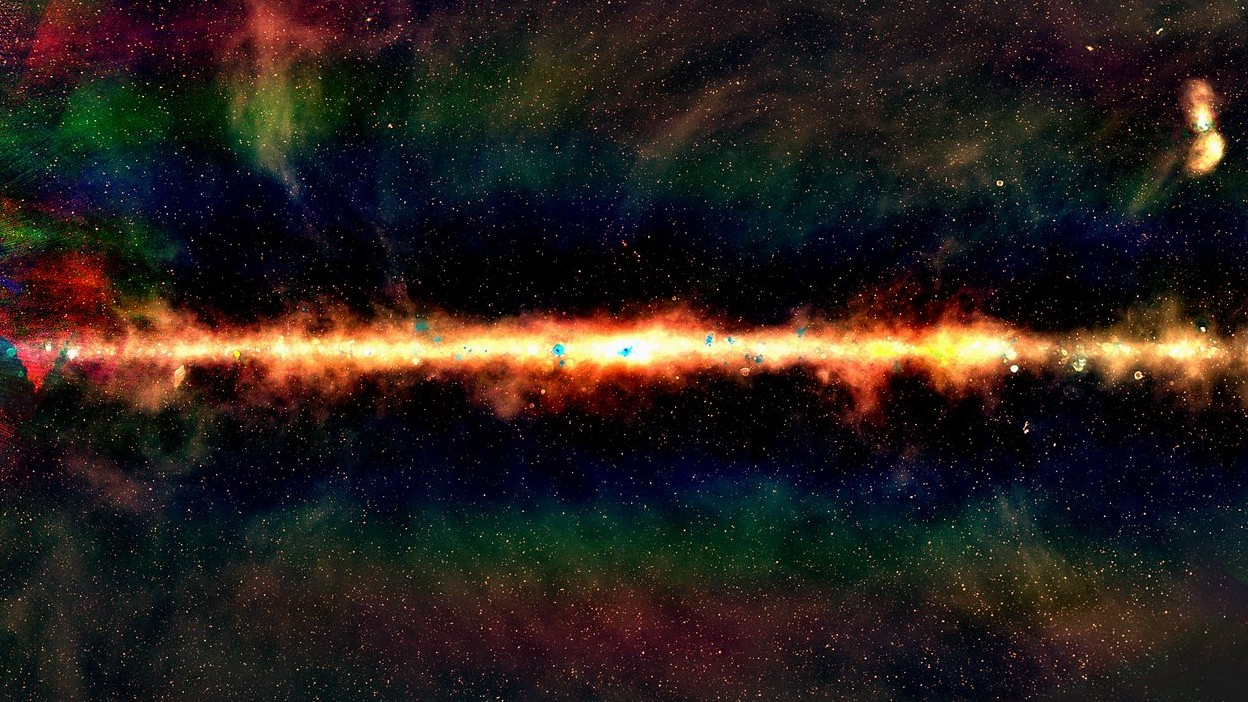
\includegraphics[width=\textwidth]{images/gleam.jpg}
        \caption[False-colour image of the radio sky from the GLEAM survey.]{\label{fig:gleam} False-colour image of the radio sky from the GLEAM survey. \citep[Image: Natasha Hurley-Walker, Curtin University/ICRAR;][]{hurley-walker_galactic_2017}}
    \end{figure}

\section{The Extragalactic Radio Sky}
\label{sec:extragalactic-radio-sky}

    The extragalactic sky appears quite different at different wavelengths. While an optical observer may look at a distant galaxy and see spirals and halos, an infrared observer will see discs and dust. What does the radio astronomer see? 
    \autoref{fig:gleam} shows a false-colour image of the radio sky from 72--231~MHz. The plane of the Milky Way is clearly visible through the centre, but nearly every other object in this image is a galaxy. These galaxies fall into two main categories: those that emit radio due to star formation (called \defn{star-forming galaxies}), and those that emit radio due to \defn{active galactic nuclei} (AGN; called \defn{radio galaxies} in this thesis). AGN can be observed at many frequencies: \DIFdelbegin \DIFdel{for }\DIFdelend \DIFaddbegin \DIFadd{For }\DIFaddend the remainder of this thesis, except where otherwise noted, `AGN' refers to \emph{radio} \DIFdelbegin \DIFdel{`AGN'}\DIFdelend \DIFaddbegin \DIFadd{AGN}\DIFaddend .

    Non-AGN emission from distant galaxies traces the recent star-formation rate (SFR). Besides low-power thermal emission, stellar radio emission from galaxies mainly comes from massive ($\gtrapprox 8$ M$_\odot$) stars \DIFdelbegin \DIFdel{, }\DIFdelend through two emission mechanisms. The first is through H~II regions, which are ionised by such stars. The ionised electrons emit bremsstrahlung radiation at radio wavelengths. The second emission mechanism is supernovae. Massive stars may end their lives in Type II and Type Ib supernovae, which can result in supernova remnants. \DIFdelbegin \DIFdel{These remnants emit }\DIFdelend \DIFaddbegin \DIFadd{Interaction between the supernova remnant and the interstellar medium (ISM) causes the emission of }\DIFaddend synchrotron radiation. Massive stars like these are short-lived (a few $10^6$ yr), and the corresponding emitting electrons have similarly short lifetimes ($\lessapprox 10^8$ yr). The radio effects of these stars are therefore also short-lived, which is why radio emission traces the recent SFR \citep{condon92radio}. Star formation-associated emission is mainly found in the \DIFdelbegin \DIFdel{disc }\DIFdelend \DIFaddbegin \DIFadd{discs }\DIFaddend of spiral galaxies, as this is where the star formation rate is highest. In particular, there is no star-forming radio emission extending outside of the galaxy proper. The radio power emitted by these galaxies at 1.4~GHz is on the order of $10^{18}$--$10^{23}$~W~Hz$^{-1}$ \citep{condon92radio}. For a radio survey like the NRAO VLA Sky Survey \citep[NVSS;][]{condon98nvss}, with a detection limit of 2.3~mJy, this luminosity range corresponds to a maximum redshift range of $0.0004$--$0.1272$ (corresponding to $6\times10^6$--$1.646\times10^9$ yr lookback time\footnote{Assuming cosmological parameters from \autoref{cha:rlfs}. Calculated using \citetitle{wright2006ned} \citep{wright2006ned}.}). Upcoming surveys such as the Evolutionary Map of the Universe \citep[EMU;][]{norris11}, with 5$\sigma$ detection thresholds of 50~$\upmu${}Jy \citep{norris11}, will push this redshift range to $0.0030$--$0.6684$ (corresponding to $4.2\times10^7$--$6.261\times10^9$ yr lookback time).

    AGN are energetic objects at the centre of galaxies, powered by accretion into supermassive black holes. The extended, strongly-magnetised plasma they eject emits synchrotron radiation from accelerating relativistic electrons, which is what we see when we observe a radio galaxy. The radio luminosity of a radio galaxy can range from $10^{20}$--$10^{28}$ W~Hz$^{-1}$ \citep{pracy16rlf} at 1.4~GHz, making them some of the most luminous objects in the Universe. They are therefore visible throughout the Universe, with the most distant AGN detected at a redshift of 7.5 \citep{banados_800-million-solar-mass_2018}. Depending on the orientation and type of AGN, as well as its interaction with its host galaxy, the radio emission may extend far beyond the galaxy itself---up to megaparsec scales---and this emission may have complex structure. Perhaps the most impressive local example is Centaurus A (Cen A), the prominent double-lobed cloud in the upper-right of \autoref{fig:gleam} extending over 8 degrees across the sky. \autoref{sec:agn} discusses AGN in more detail.

    Most \DIFdelbegin \DIFdel{radio galaxies are }\DIFdelend \DIFaddbegin \DIFadd{AGN emission is }\DIFaddend compact and unresolved in any given radio survey due to the distance at which \DIFdelbegin \DIFdel{they }\DIFdelend \DIFaddbegin \DIFadd{it }\DIFaddend can be detected and \DIFdelbegin \DIFdel{their }\DIFdelend \DIFaddbegin \DIFadd{the }\DIFaddend orientation or type \DIFaddbegin \DIFadd{of the galaxy}\DIFaddend . This means that \DIFdelbegin \DIFdel{their }\DIFdelend \DIFaddbegin \DIFadd{observed }\DIFaddend structure does not always help to distinguish AGN radio emission from star-forming radio emission. How can we tell these apart? Synchrotron emission has a considerably steeper spectral index than bremsstrahlung, but synchrotron emission dominates the bremsstrahlung in star-forming galaxies at 1.4~GHz \citep{condon92radio}. Truly star-forming galaxies can be distinguished from AGN host galaxies by using optical spectroscopy \citep[e.g.][]{mauch07rlf,groves_distinguishing_2007}, but radio emission is detectable at much greater distances than \DIFaddbegin \DIFadd{those at which }\DIFaddend good quality optical spectra can be obtained\DIFdelbegin \DIFdel{at}\DIFdelend , making this solution impractical for many galaxies. Separating star-forming galaxies from AGN host galaxies at radio wavelengths remains a difficult problem in radio astronomy.

    Polarised radio surveys can provide extra information. While radio emission due to star formation tends to not have detectable polarisation, AGN may be very strongly polarised. This makes polarisation an excellent indicator of whether a source is an AGN, though very incomplete: \DIFdelbegin \DIFdel{many AGN will also }\DIFdelend \DIFaddbegin \DIFadd{Many AGN do }\DIFaddend not have detectable polarisation, and the polarised intensity is usually less than \DIFdelbegin \DIFdel{ten }\DIFdelend \DIFaddbegin \DIFadd{10 }\DIFaddend per cent of the total radio intensity, meaning we detect far fewer polarised radio sources than we do radio sources in general.

    From the size scales described above, it should be clear that a survey of extended radio sources \DIFdelbegin \DIFdel{will be }\DIFdelend \DIFaddbegin \DIFadd{is }\DIFaddend dominated by AGN. Nevertheless, star-forming galaxies present a significant part of the radio population, and the fraction of the radio sky they comprise varies significantly with survey parameters.

\section{Radio emission}
\label{sec:radio-astronomy}

    Electromagnetic radiation in radio frequencies---about 10~MHz--1~THz \citep{condon_essential_2016}---is called \defn{radio emission}. This is a very broad range of frequencies and so radio astronomy covers a very broad range of astrophysical phenomena, from cosmological background radiation to neutron stars. The focus of this thesis is the exciting, dynamic, and so-called `violent universe' of radio galaxies. These galaxies are observed through their emission of synchrotron radiation and are studied through their observed physical structure, the intensity and spectroscopic properties of their radiation, and the polarisation and spectropolarimetric properties that are uniquely visible in radio. This section introduces synchrotron radiation and radio polarisation.

    \subsection{Synchrotron radiation}
    \label{sec:synchrotron}

        Most radio emission from radio galaxies is \defn{synchrotron radiation}, produced by relativistic charged particles accelerating in a magnetic field. A non-relativistic charged particle \DIFdelbegin \DIFdel{will spiral }\DIFdelend \DIFaddbegin \DIFadd{spirals }\DIFaddend with a fixed angular frequency when it moves in a magnetic field in a process called \defn{gyro radiation}. Synchrotron radiation is a relativistic effect: \DIFdelbegin \DIFdel{it }\DIFdelend \DIFaddbegin \DIFadd{It }\DIFaddend can be thought of as gyro radiation which has been Lorentz transformed to energies much greater than $mc^2$. The spectrum of \DIFaddbegin \DIFadd{optically thin }\DIFaddend synchrotron radiation follows a power law \citep{condon_essential_2016}:
        \begin{equation}
            \label{eq:spectral-index}
            S(\nu) \propto \nu^{\alpha}.
        \end{equation}
        where $\nu$ is the frequency of radiation and $\alpha$ is called the \defn{spectral index}\footnote{Note that the sign of $\alpha$ varies by convention, and both $S \propto \nu^{\alpha}$ and $S \propto \nu^{-\alpha}$ exist in the literature.}. It is related to the energy distribution of the emitting electrons\DIFdelbegin \DIFdel{: assuming }\DIFdelend \DIFaddbegin \DIFadd{. Assuming }\DIFaddend that the electron energy distribution follows a power law \DIFdelbegin \DIFdel{\mbox{%DIFAUXCMD
\citep[which it generally does,][]{rybicki_radiative_2008}}\hspace{0pt}%DIFAUXCMD
}\DIFdelend \DIFaddbegin \DIFadd{\mbox{%DIFAUXCMD
\citep[which it generally does;][]{rybicki_radiative_2008}}\hspace{0pt}%DIFAUXCMD
}\DIFaddend , where the number density of electrons at a given energy $E$ is given by
        \begin{equation}
            n(E) \propto E^\Gamma,
        \end{equation}
        then
        \begin{equation}
            \alpha = \frac{\Gamma - 1}{2}.
        \end{equation}
        The spectral index for synchrotron radiation tends to range from -2 to 0 \citep{condon_essential_2016} with spectral indices greater than 0 called `inverted' spectra.

    \subsection{Polarisation}
    \label{sec:polarisation}

        Electromagnetic radiation consists of waves of self-propagating, orthogonal electric and magnetic fields. The orthogonality of these two waves allows us to characterise the radiation just by the electric field. As a transverse wave, the electric field travels at an angle in the plane perpendicular to the line-of-sight. This angle and its behaviour is called the \defn{polarisation} of the wave.

        The polarisation can be characterised by decomposing the electric field into orthogonal components $E_x$ and $E_y$, letting $\hat z$ denote the axis of propagation:
        \begin{equation}
            \vec E = (\hat x E_x \exp(i \varphi_x) + \hat y E_y \exp(i \varphi_y)) \exp(i (\vec k \cdot \hat z - \omega t)).
        \end{equation}
        In an astronomical context, $\hat z$ is the line-of-sight from the source of the radiation to the observer. $\vec k$ is the \defn{wave vector} which points in the direction of travel and has magnitude $2\pi/\lambda$, and $\omega = 2\pi\nu$ is the \defn{angular frequency}. $\varphi_x$ and $\varphi_y$ are the phase offsets of each component. As this wave propagates along the line-of-sight toward an observer, the electric field oscillates in an ellipse across the $x$--$y$ plane. When the two components are in phase, this ellipse is degenerate and the radiation is called \defn{linearly polarised}. When the two components are perfectly out of phase, the ellipse is a circle, and the radiation is called \defn{circularly polarised}. Of course, any ellipse in between these extremes is also possible. For this reason, we decompose the polarisation into linearly polarised components and a circularly polarised component \DIFdelbegin \DIFdel{, }\DIFdelend called \defn{Stokes parameters} \citep{stokes_composition_1851,condon_essential_2016}. These are:
        \begin{align}
            \label{eq:stokes-i}
            I &= \frac{1}{R_0} \mathbb E_t[E_x^2 + E_y^2],\\
            \label{eq:stokes-q}
            Q &= \frac{1}{R_0} \mathbb E_t[E_x^2 - E_y^2],\\
            \label{eq:stokes-u}
            U &= \frac{1}{R_0} \mathbb E_t[2 E_x^2 E_y^2 \cos (\varphi_x - \varphi_y)],\\
            \label{eq:stokes-v}
            V &= \frac{1}{R_0} \mathbb E_t[2 E_x^2 E_y^2 \sin (\varphi_x - \varphi_y)].
        \end{align}
        $\mathbb E_t$ denotes the expectation value over time. $I$ is the \defn{total intensity} of the radiation. $Q$ and $U$ together describe the linear polarisation and \DIFdelbegin \DIFdel{together can be }\DIFdelend \DIFaddbegin \DIFadd{are }\DIFaddend used to define the \defn{polarisation angle} $\chi$:
        \begin{equation}
            \label{eq:polarisation-angle}
            \tan (2 \chi) = \frac{U}{Q}.
        \end{equation}
        $V$ is the circular polarisation and describes the eccentricity of the ellipse. For most extragalactic sources, the contribution of circular polarisation is tremendously small, especially compared to that \DIFaddbegin \DIFadd{of }\DIFaddend linear polarisation, and can be assumed to be zero \citep{rayner_radio_2000,saikia_polarization_1988}. Incoherent radiation may be composed of radiation with many different polarisations, and these polarisations may fully or partially cancel out\DIFdelbegin \DIFdel{: this }\DIFdelend \DIFaddbegin \DIFadd{. This }\DIFaddend is called \defn{unpolarised} or \DIFdelbegin \DIFdel{\defn{partially-polarised} }\DIFdelend \DIFaddbegin \DIFadd{\defn{partially polarised} }\DIFaddend radiation respectively. The total intensity of polarised radiation is called the \defn{polarised intensity} $P$ and is given by
        \begin{equation}
            \label{eq:polarised-intensity}
            P^2 = Q^2 + U^2 + V^2.
        \end{equation}
        Note that $P^2 \leq I^2$. The \defn{fractional polarisation} is the ratio between these two intensities:
        \begin{equation}
            p = \frac{P}{I}.
        \end{equation}

        The synchrotron radiation from radio galaxies is polarised, though this polarisation is not always detectable as the polarised signal tends to be much weaker than the total intensity \DIFdelbegin \DIFdel{, on the order of ten per cent \mbox{%DIFAUXCMD
\citep{osullivan_magnetic_2015}}\hspace{0pt}%DIFAUXCMD
}\DIFdelend \DIFaddbegin \DIFadd{\mbox{%DIFAUXCMD
\citep[on the order of 10 per cent;][]{osullivan_magnetic_2015}}\hspace{0pt}%DIFAUXCMD
}\DIFaddend . Additionally, the most common non-AGN cause for radio emission is star formation, which does not generally have detectable polarisation in extragalactic surveys. Polarisation is therefore an excellent way to confirm that a radio source is an AGN.

        Polarisation can also be used to describe the magnetic structure of both the radio galaxy jets and lobes as well as the intervening medium. As polarised light from distant galaxies makes its way to us, magnetised plasma along the way can cause the polarisation angle to rotate due to the Faraday effect. The amount of rotation is called the \defn{Faraday depth} $\phi$, and is related to the electron density $n_e$ and the line-of-sight magnetic field strength $\vec B \cdot \hat{z}$ of the intervening medium:
        \begin{equation}
            \label{eq:faraday-depth}
            \phi(x, y) = \frac{e^3}{8\pi^2\epsilon_0m_e^2c^3} \int_{\mathrm{there}}^{\mathrm{here}} n_e(x, y, z) \vec B(x, y, z) \cdot \mathrm{d}\hat{z}\ \mathrm{rad}\ \mathrm{m}^{-2}.
        \end{equation}
        Here $\mathrm{d}\vec r$ is the infinitesimal path length in pc \citep{brentjens_faraday_2005}. Within the synthesised beam of a radio telescope there may be multiple lines-of-sight that go through different media and hence have different Faraday depths. An example of this is a radio galaxy that is sufficiently far away that its structure is unresolved by the telescope, and yet has different polarisation properties across its breadth. The leading constant of \autoref{eq:faraday-depth} is around $2.62 \times 10^{-13}$~T$^{-1}$, more commonly written as 0.812 pc $\upmu$G$^{-1}$ cm$^{-1}$ in CGS units with $B$ in $\upmu$G and $z$ in pc. The amount of polarised radiation at each Faraday depth can be characterised by the \defn{Faraday dispersion function} (FDF) or \defn{Faraday spectrum} of the source, usually denoted $F(\phi) \in \mathbb C$. $F$ is defined implicitly by its relationship with the polarised radiation $P$ observed at wavelength $\lambda$:
        \begin{equation}
            \label{eq:faraday-dispersion-function}
            P(\lambda^2) = \int_{-\infty}^\infty F(\phi) e^{2i\lambda^2\phi}\ \mathrm{d}\phi.
        \end{equation}
        One useful way of thinking about this equation is that $F$ is the decomposition of $P(\lambda^2)$ into complex sinusoids of the form $e^{2i\lambda^2\phi}$.

        \begin{figure}
            \centering
            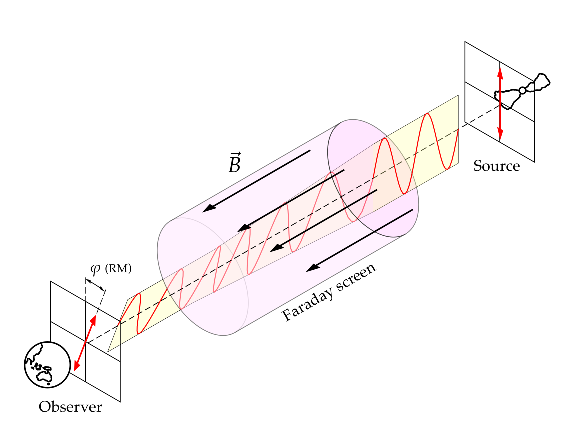
\includegraphics[width=0.8\textwidth]{images/Faraday-effect.eps}
            \caption[A Faraday screen.]{\label{fig:faraday-effect} The Faraday effect for a single Faraday screen with magnetic field $\vec B$ inducing a Faraday rotation of $\phi$. Adapted from a figure by Bob Mellish.}
        \end{figure}

        If observed radiation has precisely one Faraday depth $\phi$, then the polarised structure is called a \defn{Faraday screen} and the source is called \defn{Faraday simple}. In this degenerate case, the relationship between the polarisation angle $\chi$ and the squared wavelength $\lambda^2$ is linear:
        \begin{equation}
            \chi = \chi_0 + \phi \lambda^2,
        \end{equation}
        and the FDF is a delta distribution:
        \begin{equation}
            F(\varphi) = \delta(\varphi - \phi).
        \end{equation}
        $\phi$ is then called the \defn{rotation measure} (RM). If the source is not Faraday simple, then it is called \defn{Faraday complex}, and the question of whether a source is Faraday simple or Faraday complex is called \defn{Faraday complexity}. A diagram of a Faraday screen is shown in \autoref{fig:faraday-effect}. Until very recently, the frequency resolution of polarised surveys was insufficient to meaningfully separate most complex arrangements of Faraday depths, and so most sources were assumed to be simple and characterised entirely in terms of their rotation measure \citep[e.g.][]{taylor_rotation_2009}. Advancing telescope technology and emphasis on polarisation science has opened new frontiers in spectropolarimetry and upcoming and ongoing surveys (e.g. RACS and POSSUM) will likely report Faraday complexity and produce Faraday depth catalogues instead of rotation measures.

        If the polarised spectrum of a Faraday complex source is observed at multiple frequencies, then the multiple Faraday depths comprising it can be disentangled even though they spatially overlap in the radio image. This can provide insight into the polarised structure of the source as well as the intervening medium. This disentanglement is accomplished by inverting \autoref{eq:faraday-dispersion-function}, a process called \defn{RM synthesis} \citep{brentjens_faraday_2005}:
        \begin{equation}
            \label{eq:rm-synthesis}
            F(\phi) = \int_{-\infty}^\infty P(\lambda^2) e^{-2i\lambda^2\phi}\ \mathrm{d}\lambda^2.
        \end{equation}
        In reality we do not observe $P(\lambda^2)$ at all wavelengths nor with infinite resolution. In RM synthesis this is accounted for by the introduction of a \defn{weighting function} \citep[or \defn{windowing function}, e.g.][]{heald09faraday} $W(\lambda^2)$. $W(\lambda^2)$ is nonzero if and only if an observation was taken with wavelength $\lambda$. Substituting $P(\lambda^2) \to P(\lambda^2) W(\lambda^2)$ into \autoref{eq:rm-synthesis} results in a sum which can be numerically evaluated:
        \begin{equation}
            \label{eq:weighted-rm-synthesis}
            F(\phi) \approx \int_{-\infty}^\infty P(\lambda^2) W(\lambda^2) e^{-2i\lambda^2\phi}\ \mathrm{d}\lambda^2 = \sum_{j = 1}^J P(\lambda^2_j) W(\lambda^2_j) e^{-2i\lambda^2_j\phi}.
        \end{equation}
        $P(\lambda^2_j)$ is the observed polarisation at the $j$th value of wavelength, $W(\lambda^2_j)$ is the corresponding $j$th weight, and $J$ is the total number of wavelengths for which measurements were taken. The weighting function $W$ is analogous to the weighting function in radio synthesis imaging. The most common choices of $W$ are 1) uniform weighting\footnote{The analogous weighting scheme in radio synthesis imaging would be natural weighting \DIFdelbegin \DIFdel{, }\DIFdelend rather than uniform---an unfortunate overlap in terminology.} with $W(\lambda_j^2) = 1$ for all nonzero values, and 2) weighting by the inverse variance at each wavelength.

        Of course, no physical source has a precise Faraday depth, as there is always intrinsic scatter. Along the \DIFdelbegin \DIFdel{line of sight}\DIFdelend \DIFaddbegin \DIFadd{line-of-sight}\DIFaddend , if we assume \DIFdelbegin \DIFdel{Gaussian noise in an otherwise-constant }\DIFdelend \DIFaddbegin \DIFadd{that }\DIFaddend $n_e$ \DIFaddbegin \DIFadd{is observed with random Gaussian noise }\DIFaddend i.e. $n_e(z) \sim \mathcal N(\overline n_e, \sigma_{n_e}^2)$, and \DIFdelbegin \DIFdel{a constant }\DIFdelend \DIFaddbegin \DIFadd{that }\DIFaddend $B$ \DIFaddbegin \DIFadd{is constant }\DIFaddend for simplicity, then we find\DIFaddbegin \DIFadd{:
        }\DIFaddend \begin{equation}
            \phi \sim \mathcal N\left(\frac{e^3}{8\pi^2\epsilon_0m_e^2c^3} B \overline n_e, \frac{e^3}{8\pi^2\epsilon_0m_e^2c^3} B \sigma_{n_e}^2\right),
        \end{equation}
        that is, the depth has an uncertainty proportional to the magnetic field strength and the noise in $n_e$. A similar result follows for noise in $B$ only. There is no analytic solution for noise in both $B$ and $n_e$, but if we approximate the integrand as a Gaussian by calculating the mean and variance, we find\DIFaddbegin \DIFadd{:
        }\DIFaddend \begin{equation}
            \phi \sim \mathcal N\left(\frac{e^3}{8\pi^2\epsilon_0m_e^2c^3} \frac{\overline n_e \sigma_B^2 + \overline B \sigma_{n_e}^2}{\sigma_B^2 + \sigma_{n_e}^2}, \frac{e^3}{8\pi^2\epsilon_0m_e^2c^3} \frac{\sigma_{n_e}^2 \sigma_B^2}{\sigma_{n_e}^2 + \sigma_B^2}\right).
        \end{equation}
        We observe multiple lines-of-sight that are coalesced into one within the beam. Due to this noise, even with constant $n_e$ and $B$ across a source, we can see multiple Faraday depths as each line-of-sight is a sample from the above distribution.

    % \item the extra-galactic radio sky (gotta start here to be interesting?): \begin{itemize}
    %     \item star-forming galaxies
    %     \item AGN
    %     \item the galactic plane and foreground
    % \end{itemize}

    % The last major component of the radio sky is the galactic plane of the Milky Way.

    % \begin{itemize}
    %     \item how often do we expect to see AGN vs. star formation?
    %     \item how is this affected by observational parameters?
    %     \item how do we tell the difference?
    %     \item extended sources are mainly AGN in the surveys we care about
    %     \item what gets in our way of seeing extragalactic stuff?
    % \end{itemize}

\section{Radio galaxies and active galactic nuclei}
\label{sec:agn}
    % \begin{itemize}
    %     \item AGN: \begin{itemize}
    %         \item jets
    %         \item lobes
    %         \item the unified model
    %         \item classes including FRI and FRII, radio loud and radio quiet... etc
    %         \item polarisation structure
    %         \item spectral index
    %         \item environmental interaction with jets and lobes, including how much power they inject according to simulations and literature
    %         \item host galaxies
    %     \end{itemize}
    %     \item AGN throughout the Universe: \begin{itemize}
    %         \item expected RLF/distribution
    %         \item getting brighter back in time
    %         \item FRI/FRII? radio loud, radio quiet?
    %         \item how many AGN are there?
    %         \item how do AGN tie into galaxy evolution and feedback?
    %     \end{itemize}
    % \end{itemize}

    AGN are some of the most energetic objects in the Universe. They both provide a laboratory for extreme physics and are a key part of the life cycle of a galaxy \citep{heckman_coevolution_2014}. Powered by a supermassive black hole, they convert gravitational potential energy into intense electromagnetic radiation at a broad range of frequencies. AGN that produce strong radio emission are called radio AGN, and methods of observing the complex structures that these radio AGN form as radio galaxies are the focus of this thesis.

    \subsection{What we see when we look at AGN}
    \label{sec:what-we-see-agn}

        Observations are the crux of astronomy. While there are many models of how AGN evolve and how they interact with their surroundings---and indeed, the actual structure of an AGN is very much an open question in astronomy---the evidence presented by observations is reliable and a good place to start discussing the structure, behaviour, and importance of AGN throughout the Universe.

        \begin{figure}
            \centering
            \begin{subfigure}{0.45\textwidth}
                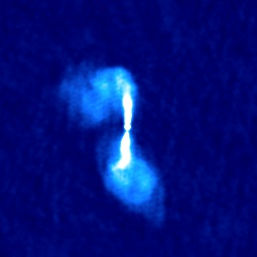
\includegraphics[width=\textwidth]{images/3C_272-1.jpg}
                \caption{M84/3C 272.1}
                \label{fig:m84}
            \end{subfigure}
            \begin{subfigure}{0.45\textwidth}
                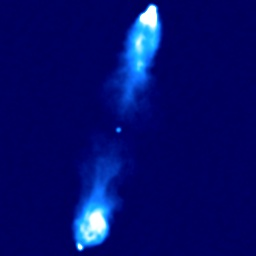
\includegraphics[width=\textwidth]{images/3C_223.jpg}
                \caption{3C 223}
                \label{fig:3C223}
            \end{subfigure}
            \caption[Examples of a FRI and a FRII radio galaxy.]{\label{fig:fri-frii} Examples of (a) a FRI \citep{laing_rotation_1987} and (b) a FRII radio galaxy \citep{leahy_vla_1991}. Both are shown with an arcsinh stretch and were observed with the VLA.}
        \end{figure}

        As powerful sources of radio emission, radio AGN and their associated extended structure can be seen throughout the Universe. Sufficiently close or large radio galaxies can be resolved by telescopes and their structure examined, while more distant or smaller radio galaxies may be unresolved and point-like. A well-resolved radio galaxy can be a striking thing: \DIFdelbegin \DIFdel{from }\DIFdelend \DIFaddbegin \DIFadd{From }\DIFaddend the central AGN extend two opposing, tightly-collimated jets, which widen into huge lobes of radio-bright plasma. These lobes may have further structure, particularly bright regions called \defn{hot-spots}, and the jets and lobes may be bent and distorted as they travel away from their host galaxy. For any given radio galaxy, some of these features may or may not be present. In particular, radio galaxies are often divided into two classes based on the kinds of extended structure that are visible, called Fanaroff-Riley type I (FRI) and Fanaroff-Riley type II (FRII) radio galaxies. FRI have wavy, diffuse lobes, appearing brighter toward the host galaxy and dimming further out (e.g. \autoref{fig:m84}). FRII, on the other hand, have long, tightly-collimated jets and sharp-edged lobes with bright hot-spots \citep{urry95unified} at the very end of the lobes, and are brighter further away from the host galaxy (e.g. \autoref{fig:3C223}). FRII are also generally higher-luminosity \citep{fanaroff1974} than FRI, and therefore make up the majority of observed extended radio sources throughout the Universe. However, this is by no means the clear-cut divide it was once thought to be \citep{mingo_revisiting_2019} with the difference now being attributed largely to environmental effects rather than jet power. The current understanding is that FRII jets remain at relativistic energies up until the edge of the lobe, where they terminate in a shock that appears as a hot-spot, while FRI jets decelerate within the galaxy itself \citep{hardcastle20feedback}. This sharp difference in extended structure begins with environmental interactions at the very centre of the galaxy.

        A radio galaxy can be tremendously extended, with increasingly many radio galaxies being found with a length of over one megaparsec. Such large galaxies are called \defn{giant radio galaxies}, but even non-giants are still quite big, regularly extending well outside the stellar component of the host galaxy. We will discuss the extended structure in \autoref{sec:extended-structure-of-agn}. \DIFdelbegin %DIFDELCMD < \autoref{sec:rlfs-giants} %%%
\DIFdelend \DIFaddbegin \aref{sec:rlfs-giants} \DIFaddend lists some giants discovered during the work of this thesis.

        An AGN interacts with its host galaxy, and so the host galaxy of an AGN can also provide interesting insights into the structure and behaviour of the AGN. Early research indicated that the split between FRI and FRII radio galaxies was dependent on the mid-infrared and optical brightness (and therefore density) of the host galaxy \citep{ledlow_20_1996,bicknell_relativistic_1995} though more recent work suggests this may not be a strong effect if it exists at all \citep{hardcastle20feedback}. \autoref{cha:rlfs} investigates the distribution of radio luminosities conditioned on the mid-infrared colour of the host galaxy.

    \subsection{Extended structure}
    \label{sec:extended-structure-of-agn}

        The jets and lobes of AGN can be very extended, with the largest known radio galaxies measuring over 4 Mpc end-to-end \citep{machalski_understanding_2011}. This is a much larger size than the radii of the host galaxies, and so the jets and lobes of AGN are uniquely posed to interact with the local environment. Environmental interactions both within and outside the host galaxy warp and distort the jets and lobes. Within the galaxy, the jets drive a bubble of energy in the \DIFdelbegin \DIFdel{interstellar medium \mbox{%DIFAUXCMD
\citep[ISM;][]{mukherjee_relativistic_2016}}\hspace{0pt}%DIFAUXCMD
}\DIFdelend \DIFaddbegin \DIFadd{ISM \mbox{%DIFAUXCMD
\citep{mukherjee_relativistic_2016}}\hspace{0pt}%DIFAUXCMD
}\DIFaddend , transferring energy into the ISM with different effects depending on the jet power \citep{mukherjee_relativistic_2018}; the ISM on the other hand suppresses the jets and distorts them to varying amounts depending on the degree of interaction \citep{mukherjee_relativistic_2018}. Outside the galaxy, the jets and lobes are bent by the intra-cluster medium and neighbouring galaxies \citep[ICM;][]{garon19bending,rodman19asymmetry} and this structure may even be used as a probe for cluster environments \citep{banfield_radio_2016,sakelliou_3c40_2008}.

        \begin{figure}
            \centering
            \begin{subfigure}{0.3\textwidth}
                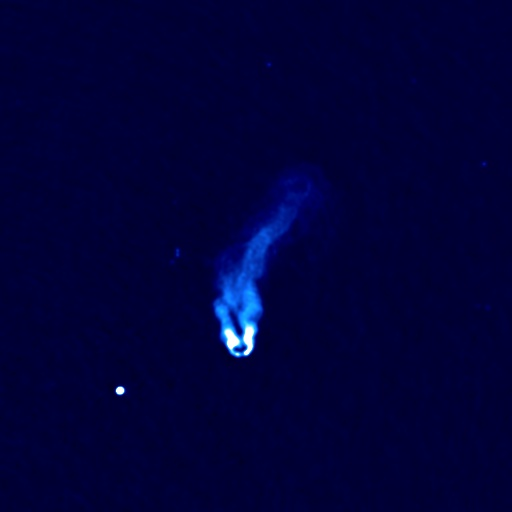
\includegraphics[width=\textwidth]{images/3C_83-1B.jpg}
                \caption{3C 83.1B}
                \label{fig:3C83-1B}
            \end{subfigure}
            \begin{subfigure}{0.3\textwidth}
                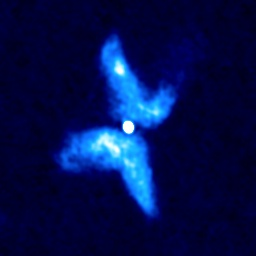
\includegraphics[width=\textwidth]{images/3C_315.jpg}
                \caption{3C 315}
                \label{fig:3C315}
            \end{subfigure}
            \begin{subfigure}{0.3\textwidth}
                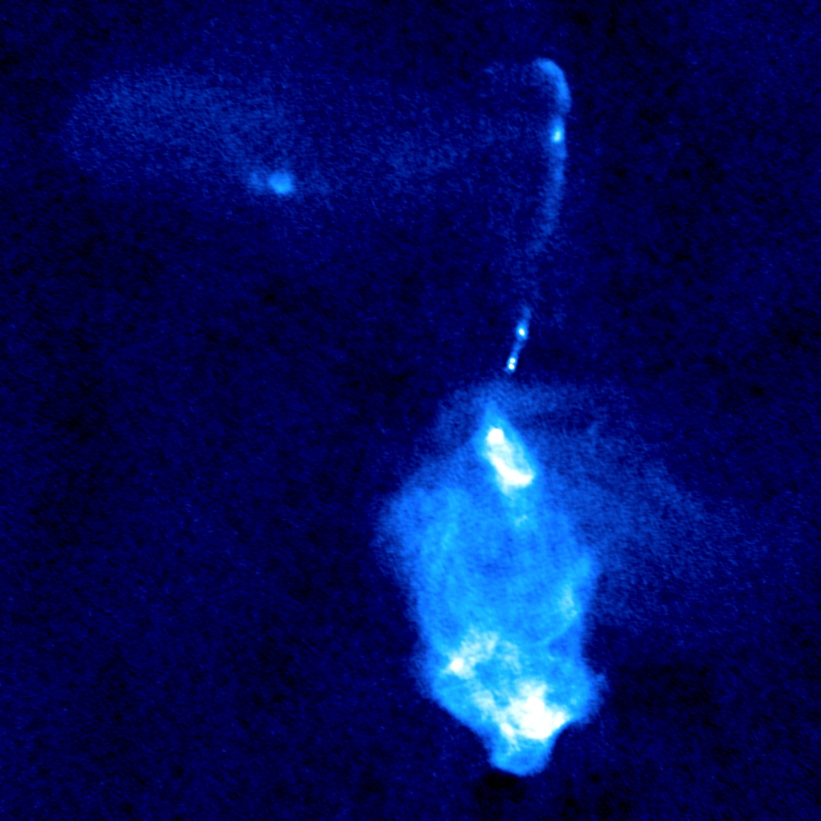
\includegraphics[width=\textwidth]{images/3C_433.jpg}
                \caption{3C 433}
                \label{fig:3C433}
            \end{subfigure}
            \caption[Three radio galaxies with interesting structure.]{Radio galaxies, displayed with an arcsinh colour scale. All images were taken with the VLA. (a) is a narrow-angled tail radio galaxy \citep{leahy_atlas_nodate}, (b) is an X-shaped radio galaxy \citep{leahy_polarization_1986}, and (c) is a very unusually-shaped radio galaxy \citep{black_study_1992}.}
            \label{fig:interesting}
        \end{figure}

        The strong interaction of AGN with their \DIFdelbegin \DIFdel{environment }\DIFdelend \DIFaddbegin \DIFadd{environments }\DIFaddend leads to a great variety of exotic-shaped radio galaxies. Some morphological classes of this `radio galaxy zoo' include X-shaped galaxies, which have two sets of lobes roughly perpendicular to each other; wide- and narrow-angled tail galaxies, which are bent about the core with large and small angles respectively; head-tail galaxies, which are so bent that the two lobes seem to be the same or nearly the same; double-doubles, which have two sets of lobes on each side; and many, many more. Some examples of radio galaxies with interesting structure are shown in \autoref{fig:interesting}. Large-scale automated identification of these galaxies can be tricky owing to their variety, extent, and often disconnected structure.

        AGN cores tend to have flat or inverted spectral indices around -0.5--1 \citep{condon_essential_2016,randall_spectral_2012}. Moving out from the host galaxy, the spectral index steepens as the electrons are older and less energetic, with the spectral index of the lobes usually at about -0.7 \citep{condon_essential_2016}. The hot-spots of FRII galaxies have spectral indices between -0.5 -- -0.7, becoming shallower as the electrons reaccelerate. These are only general trends: \DIFdelbegin \DIFdel{the }\DIFdelend \DIFaddbegin \DIFadd{The }\DIFaddend spectral structure within lobes can be very complex \citep{treichel_spectral_2001}. The jets do not strongly emit and are only detectable for particularly deep observations or nearby radio galaxies.

    \subsection{The unified model}
    \label{sec:unified-model}

        \begin{figure}
            \centering
            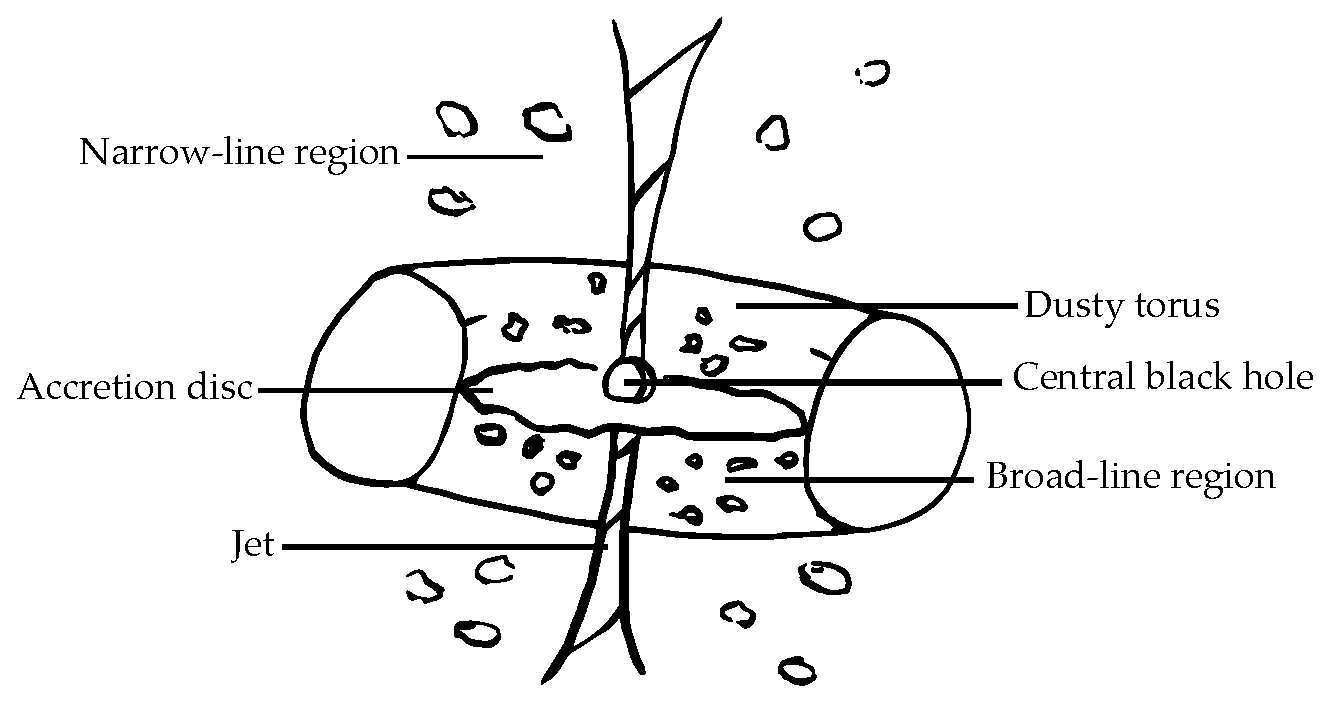
\includegraphics[width=\textwidth]{images/agn.eps}
            \caption{\label{fig:agn} The unified model of AGN.}
        \end{figure}

        At their core, AGN are an accreting \defn{supermassive black hole}: a body so dense that even light cannot escape its gravitational pull, with mass on the order of $10^7$--$10^9\ \mathrm{M}_\odot$ \citep{marconi_relation_2003}. Such black holes seem to exist at the centres of galaxies and these galaxies are called \defn{host galaxies}. The current understanding of the structure of an AGN is as follows \citep{urry95unified}. The black hole is surrounded by an accretion disc emitting in ultraviolet and X-ray. Beyond this is the broad-line region, named for the Doppler-broadened emission lines emitted by the energetic clouds of material surrounding the accretion disc. The broad-line region and accretion disc are themselves surrounded by a dusty torus (or some other disc-like structure) which prevents light from the centre of the AGN being observed from the sides. Further still from the accretion disc is the narrow-line region, where lower-energy gas produces narrow emission lines. From either side of the disc, an AGN produces two collimated outflows of relativistic plasma called {jets}, and these jets may interact with gas in the host galaxy to produce bright radio emission. The jets are not always visible. As the jets disperse further out from the centre of the AGN they widen into plumes of plasma known as \defn{lobes}. This model of AGN unifies different observed classes of AGN by their orientation and luminosity, and is hence known as the \defn{unified model} \citep{antonucci_unified_1993}. Recent work suggests that the unified model of AGN is not the full story \citep[e.g.][]{zhuang_interplay_2020}.

        There are many different ways to divide the set of radio AGN into classes. By morphology, radio AGN are often divided by the structure of the jets and lobes, with FRI and FRII the most striking examples. AGN can also be divided into \defn{radiative-mode} and \defn{jet-mode} by how they expel their energy \citep{heckman_coevolution_2014}. Radiative-mode AGN produce radiative energy in amounts higher than 1 per cent of their Eddington limit, while jet-mode AGN mainly output energy through their jets. The Eddington limit describes the maximum luminosity that a compact object can emit, and is given in \autoref{eq:eddington} \citep{rybicki_radiative_2008}:
        \begin{equation}
            L_{\mathrm{Eddington}}(M) = \frac{4\pi G M m_p c}{\sigma_T}
            \label{eq:eddington}
        \end{equation}
        where $M$ is the mass of the compact object.

        Optical emission observed near the centre of the AGN can be used to divide radio AGN into broad-line and narrow-line galaxies. The former have broad spectral lines while the latter have narrow spectral lines, with broader spectral lines indicative of higher thermal energies. The most common interpretation, under the unified model, is that broad-line AGN are those seen end-on and narrow-line are those seen edge-on with the dusty torus obscuring the broad-line region. These narrow-line galaxies are usually the only ones for which we see significant extended structure.

    \subsection{Polarised structure}
    \label{sec:polarised-structure-of-agn}

        The magnetic field of AGN is thought to be critical to their structure \citep{sikora_magnetic_2013}. A strong magnetic field is required to eject and collimate the jets \citep{lovelace_dynamo_1976} and the magnetic environment influences the structure of the jets \citep{osullivan_magnetic_2015}. Polarisation provides a probe for measuring this magnetic field. Radiative- and jet-mode AGN have different fractional polarisations, with jet-mode AGN having a much wider range of fractional polarisations ($p \sim [0, 30]$ per cent) compared to radiative-mode AGN (limited to $p \lessapprox 15$ per cent), with this difference attributable to the magnetic environment \citep{osullivan_magnetic_2015}. Steep-spectrum ($\alpha > 0.5$) and flat-spectrum ($\alpha < 0.5$) AGN have differing fractional polarisations, with steep-spectrum sources having much higher fractional polarisation for frequencies $> 5$~GHz and flat-spectrum sources having higher fractional polarisation for frequencies $< 1$~GHz due to frequency-dependent depolarisation of the steep-spectrum sources \citep{saikia_polarization_1988}. \DIFdelbegin \DIFdel{Hotspots }\DIFdelend \DIFaddbegin \DIFadd{Hot-spots }\DIFaddend of FRII radio galaxies have low polarisation ($<10$ per cent) while the more diffuse sections may have much greater polarisation ($>20$ per cent) \citep{saikia_polarization_1988}. The direction of the magnetic field is correlated with the direction of \DIFaddbegin \DIFadd{patterns in }\DIFaddend the total intensity of the source \citep{saikia_polarization_1988}.

    \subsection{AGN luminosity}
    \label{sec:agn-throughout}

        \begin{figure}
            \centering
            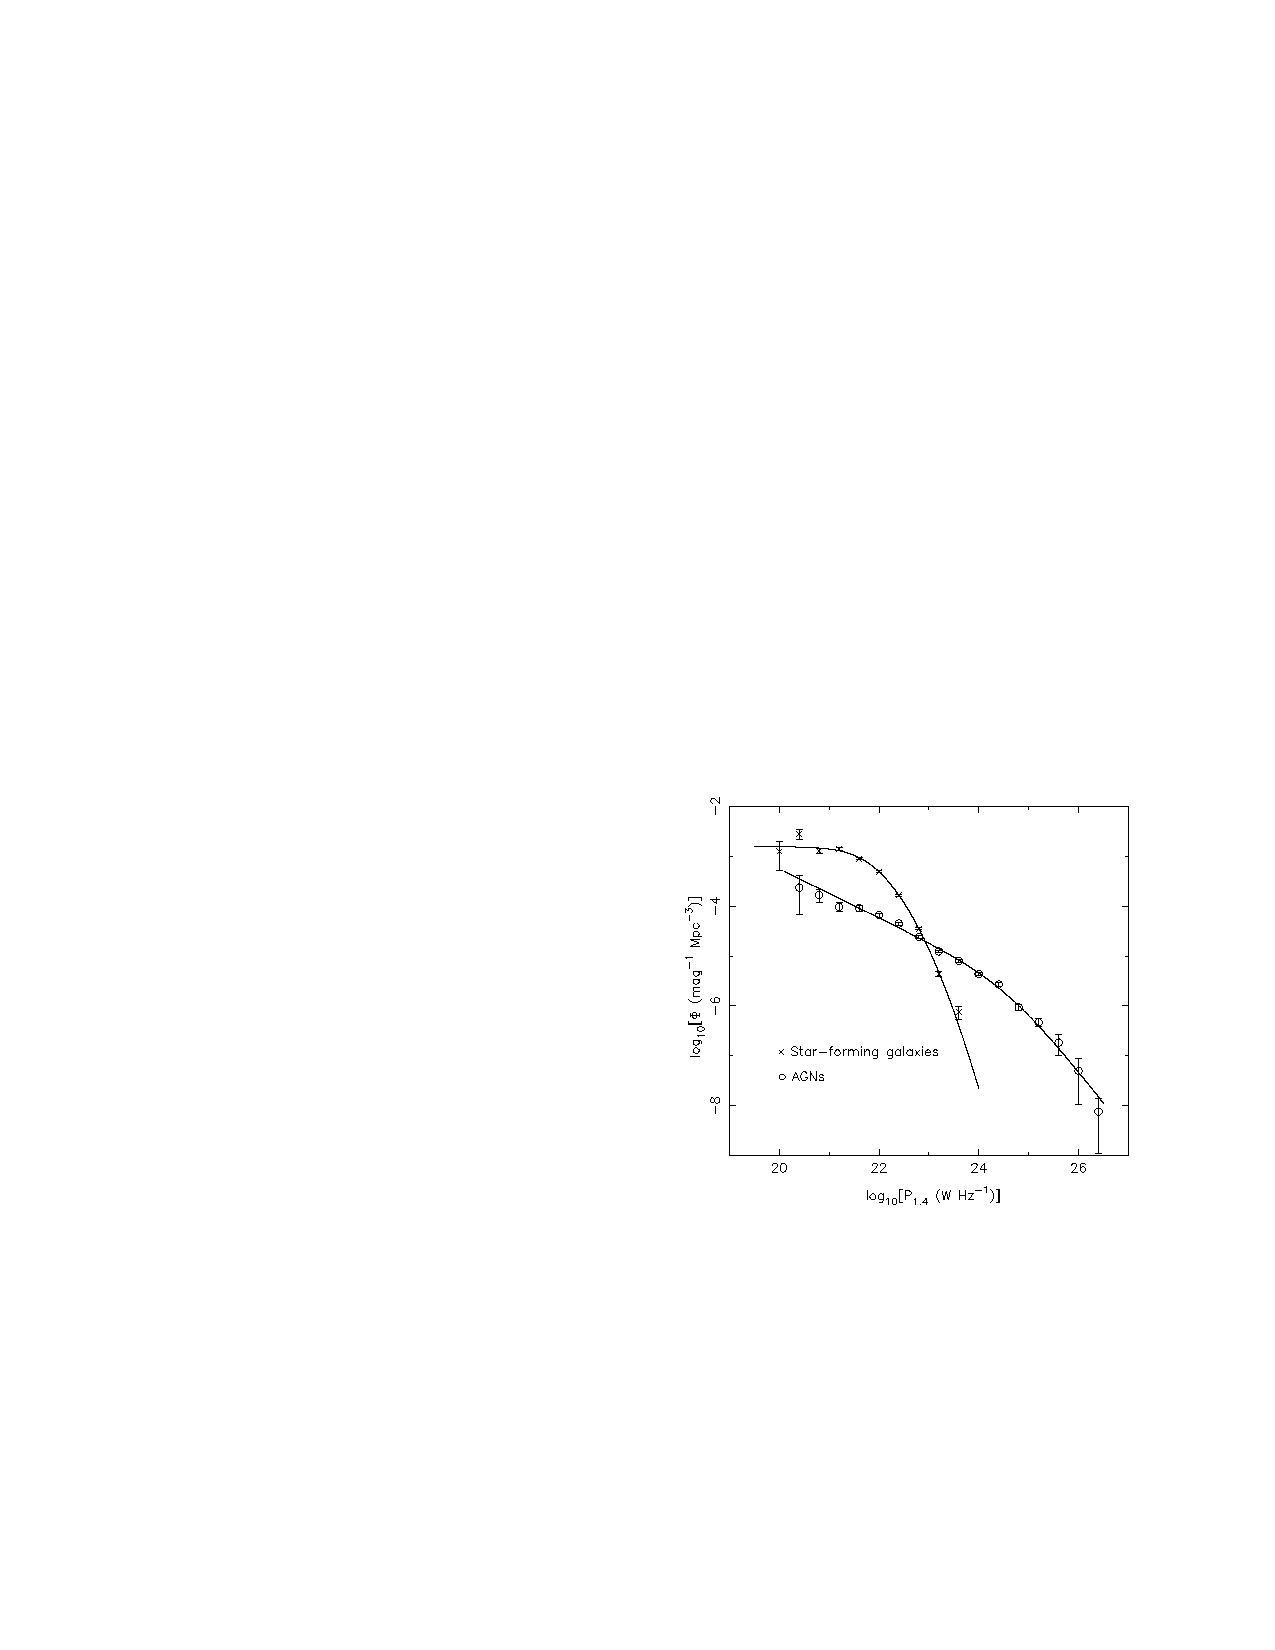
\includegraphics[width=0.7\textwidth]{images/mauch07rlf.pdf}
            \caption{\label{fig:mauch-rlf} RLF for star-forming galaxies and AGN, from \citet{mauch07rlf}.}
        \end{figure}

        The distribution of AGN luminosities throughout the Universe can be characterised by the \defn{radio luminosity function} (RLF). This describes the density of AGN within luminosity bins at a given frequency. The RLF at 1.4~GHz from \citet{mauch07rlf} is shown in \autoref{fig:mauch-rlf}. 1.4~GHz is arguably the most common large-scale survey frequency as it detects the easily observed 21~cm hydrogen line, but this RLF can be scaled to different frequencies by assuming a constant spectral index ($\alpha = -0.7$ for a typical AGN). In \autoref{cha:rlfs}, we will use a machine learning-derived radio source catalogue to estimate a RLF for extended radio objects.

    \subsection{The role of AGN}
    \label{sec:role-of-agn}

        AGN are an important part of galaxy evolution, though the exact mechanisms of this are not currently known. Understanding galaxy evolution requires understanding the links between it and AGN, and thus requires the study of AGN.

        There are established relationships between AGN parameters and galaxy parameters: \DIFdelbegin \DIFdel{the }\DIFdelend \DIFaddbegin \DIFadd{The }\DIFaddend mass of the central black hole is correlated with the stellar mass and velocity dispersion near the core in elliptical galaxies \citep{cattaneo_role_2009} as well as the luminosity of the bulge \citep{kormendy_inward_1995}. Massive galaxies seem to be more likely to contain an AGN rather than an inactive galactic nucleus \citep{hardcastle20feedback}. The large-scale behaviour of AGN (e.g. the Fanaroff-Riley divide) may be caused by interactions within the host galaxy \citep{hardcastle20feedback} and this interaction would be a significant energy contribution to the \DIFdelbegin \DIFdel{interstellar medium}\DIFdelend \DIFaddbegin \DIFadd{ISM}\DIFaddend .

        Perhaps the biggest topic in this field is that of \defn{AGN feedback}, the role of AGN in the enhancement or quenching of star formation within their host galaxies. Star formation requires cold gas; AGN can push gas out of the galaxy \citep{zubovas_clearing_2012} or heat it so that it can no longer form stars. But the rapid expansion of AGN jets can produce shocks in the local environment, compressing gas, triggering collapse of gas clouds, and potentially increasing the star formation rate \citep{zubovas_collapse_2014}.

        For a review of the role of AGN within galaxy evolution, see \citet{kormendy_coevolution_2013}. For a detailed review of the current understanding of AGN, see \citet{hardcastle20feedback}.

\section{Classifying AGN}
\label{sec:classification-of-agn}

    As discussed in \autoref{sec:unified-model}, radio galaxies fall into many classes. Understanding the mechanisms underlying these class distinctions is critical to understanding AGN. As we have no way to directly see the core of an AGN (it's far too small to resolve at the distances AGN occur and may also be occluded), our only method to investigate AGN is to look at their large-scale behaviour. Some classes may relate to the fundamental AGN core, some may be environmental, and some may be due to observation effects. Much of our knowledge about AGN (such as the unified model) come from analysing these classes and their differences. To investigate classes of AGN a large sample of each class is required, and source classification approaches can divide a large dataset from a radio survey into useful subsets. Knowing what class a source is may also help analyse its properties as we can estimate its expected behaviour, perhaps with the aid of models and simulations. Some classes may have interesting structure or properties that can only be observed with additional detailed observations, so identifying which sources require follow-up is a tightly related problem in radio astronomy. An excellent, though now somewhat dated, summary of radio source classification is the review paper by \citet{urry95unified}, which we recommend for further reading.

    Deciding which class a given radio galaxy falls into may be challenging, and doing this automatically even more so. This section discusses approaches to classifying radio galaxies.

    \subsection{Statistical and manual classification of AGN}
    \label{sec:manual-classification}

        Manual and statistical approaches to classifying AGN have dominated the radio astronomy literature until very recently, due to the comparative lack of computational power as well as a lack of good automated methods. Manual methods amount to examining the structure of a resolved source and determining its class\DIFdelbegin \DIFdel{: this }\DIFdelend \DIFaddbegin \DIFadd{. This }\DIFaddend is how we usually identify bent radio galaxies, head-tail radio galaxies, X-shaped radio galaxies, and those radio galaxies with more unusual morphologies. Statistical approaches identify properties of the source that can be combined and thresholded to separate the sources into categories en masse. Modern machine learning techniques for classification of radio sources can be thought of as an extension of these statistical methods, where the properties and their combinations are identified automatically, but we will discuss these separately in \autoref{sec:ml-classification-of-agn}.

        Arguably the most well-known radio classification scheme, FRI and FRII, was originally defined on well-resolved radio galaxies by computing the ratio of the distance between the regions of highest brightness on opposite lobes and the total extent of the radio emission \citep{fanaroff1974}. Sources with a ratio under 0.5 were called FRI and those with a ratio greater than 0.5 were called FRII. This classification has over time evolved into a less precise divide, with classification generally now morphological and based on the structure (diffuse, wavy plumes versus hot-spots and lobes for FRI and FRII respectively). The FRI and FRII divide has been further complicated by other related categorisations such as the so-called ``Fanaroff-Riley type 0'' sources which seem to be the lower end of a continuum of radio sources with diffuse plumes \citep{garofalo_fr0_2019,capetti_lofar_2020} as well as hybrid morphology radio sources (HyMoRS) which appear to be FRI on one side and FRII on the other \citep{gopal-krishna_extragalactic_2000,kapinska_radio_2017}. Many classes are defined by explicitly statistical means; for example, steep- and flat-spectrum sources are divided by spectral index at $\alpha = 0.5$ \citep{urry95unified}. For convenient analysis, radio sources are often also grouped into ``observational'' classes that don't have a physical analogue based on their apparent structure, e.g. the GLEAM survey classifies radio sources into the number of apparent components, which is highly dependent on the observational parameters \citep{white_gleam_2020}.

        More unusual or more loosely defined classes, such as X-shaped radio galaxies and giants, have often been identified by manual searches through large datasets, e.g. \citet{cheung_first_2007,dabhade_search_2020}\DIFaddbegin \DIFadd{, }\DIFaddend and notably the recent ROGUE I catalogue of 32~616 morphologically classified radio galaxies \citep{zywucka_catalogue_2020}. These searches are often aided by computer algorithms \citep[e.g.][]{proctor_morphological_2011,dabhade_search_2020}.

        Radio sources are also more generally classified, such as into AGN or non-AGN emission \citep{koziel-wierzbowska_identifying_2020}, often using optical emission lines or optical/infrared magnitude.

    \subsection{Machine learning classification of AGN}
    \label{sec:ml-classification-of-agn}

        Machine learning based approaches for radio source classification are rapidly evolving as the amount of radio data available through big surveys increases. Advances in tooling, such as the wide availability of hardware-accelerated automatic differentiation software, have also contributed to an explosion in machine learning applications in astronomy by making machine learning techniques more available to astronomy researchers.

        Morphological classification of galaxies with machine learning began in optical astronomy, probably due to the large sample sizes of well-resolved galaxies previously available. The earliest such paper is likely the application of neural networks to the task by \citeauthor{storrie-lombardi_morphological_1992} in 1992. From here, the field applied other classification algorithms such as decision trees \citep[e.g.][]{owens_using_1996}. The Sloan Digital Sky Survey (SDSS) brought an explosion of new data in 2003, and new experiments in classification soon followed \citep[e.g.][]{ball_galaxy_2004,ball_robust_2006}. The Galaxy Zoo project leveraged hundreds of thousands of volunteers to produce an astonishingly large set of labelled optical galaxies from SDSS and subsequent papers used this as a training set for machine learning methods \citep{banerji_galaxy_2010,dieleman15cnn,zhu_galaxy_2019}.

        While machine learning has been used in radio astronomy for some time \DIFdelbegin \DIFdel{\mbox{%DIFAUXCMD
\citep[e.g. the NVSS used neural networks to detect sidelobes;]{condon98nvss} }\hspace{0pt}%DIFAUXCMD
}\DIFdelend \DIFaddbegin \DIFadd{\mbox{%DIFAUXCMD
\citep[e.g. the NVSS used neural networks to detect sidelobes;][]{condon98nvss} }\hspace{0pt}%DIFAUXCMD
}\DIFaddend its first application to radio source classification was most likely to identifying quasar candidates \citep{carballo_selection_2004} in Faint Images of the Radio Sky at Twenty Centimeters \citep[FIRST;][]{becker95first}. \citet{proctor06} applied decision tree ensembles to identify bent double morphologies in FIRST, manually selecting features to characterise radio sources, while \citet{bastien_classifying_2017} used shapelet analysis to obtain features to feed into their decision tree ensembles. 2011--12 marked a revolution in computer vision with the discovery that deep convolutional neural networks \citep[known as early as 1989, see][]{lecun_backpropagation_1989}, boosted dramatically by widely available training data generated by the internet and a huge increase in computational power from GPUs, could achieve greater-than-human performance on image classification tasks. Deep neural networks have since found use for morphological classification of radio sources, such as FRI vs. FRII \parencites{aniyan17cnn,ma_machine_2019,lukic_morphological_2019,tang_transfer_2019,samudre_data-efficient_2020,bowles_attention-gating_2020}[see also][]{ma_radio_2018}, compact vs. extended sources \citep{lukic18compact,alhassan_first_2018,lukic_morphological_2019}, and observational classes \citep{galvin19som,ralph19ae}.

        There are also many works on classification of radio sources besides morphology. Machine learning has been applied to AGN classification tasks including blazar classification \citep{arsioli_machine_2020} and radio loudness \citep{beaklini_agn_2020}. Deep learning is also prevalent on this topic, with deep learning finding applications in Faraday complexity classification \citep{brown_classifying_2018} and notably in transient detection \citep{connor_applying_2018,guo_pulsar_2019,wang_pulsar_2019,agarwal_fetch_2020,lin_pulsar_2020,zhang_applying_2020,balakrishnan_pulsar_2020}.

        It is worth contrasting these machine learning approaches with non-machine learning automated approaches, as the two are often conflated in the literature. \citet{mingo_revisiting_2019}, for example, use an automated version of detecting the brightness gradient of extended radio sources to determine whether they are FRI or FRII en masse and apply this approach to the LoTSS survey. \citet{segal_identifying_2019} apply an information theoretic approach to estimating morphological complexity of a source. The key difference between a machine learning automated approach and a non-machine learning automated approach is that the former has the capacity to change its behaviour based on available data, while the latter does not---though note that this is not necessarily a bad thing.

\section{Cross-identification}
\label{sec:xid}

    \defn{Cross-identification} is the problem of matching an observed astronomical object at one wavelength with its counterpart in a survey at some other wavelength. Sometimes the counterpart in question can be obvious, such as when the object being matched is compact and well-aligned in both wavelengths. This is not the case for radio, though: \DIFdelbegin \DIFdel{radio }\DIFdelend \DIFaddbegin \DIFadd{Radio }\DIFaddend galaxies can be very extended and, due to environmental interactions, this extended structure may be complicated and have no obvious relationship to the galaxy at other wavelengths. The galaxy itself in radio cross-identification is called the \defn{host galaxy} as it hosts the central AGN.

    \subsection{Why do we need to cross-identify?}
    \label{sec:xid-why}

        Radio spectra do not generally contain much information besides the spectral index: as Jim Condon purportedly said, "There's nothing as useless as a radio source". Most information about extragalactic sources is gleaned from other wavelengths, with optical and infrared showing physically meaningful differences due to emission and absorption at these wavelengths. For this reason radio sources are typically cross-identified with their counterparts at other wavelengths to get information. Key features of a host galaxy that may be obtained from optical or infrared observations include its redshift, mass, star formation rate, and composition. From these we may also determine properties of the radio plasma, most notably its physical extent and radio luminosity, both of which require knowing the redshift.

    \subsection{Methods for cross-identification}
    \label{sec:xid-how}

        \begin{sloppypar}
        Most small radio surveys are cross-identified by astronomers, visually comparing the radio image to the optical or infrared image \citep[e.g.][]{norris06,middelberg08}. The largest such catalogue is the ROGUE~I catalogue with over 32~000 cross-identifications \citep{zywucka_catalogue_2020}. The Radio Galaxy Zoo project \citep{banfield15} extended manual cross-identification to larger scales by crowdsourcing, asking volunteers online to cross-identify FIRST and ATLAS resulting in 75~000 cross-identified extended sources. This is the largest manually cross-identified source catalogue ever, by citizen scientists rather than professional astronomers---though this distinction does not seem to matter as the accuracy of cross-identifications in Radio Galaxy Zoo is still quite high, and there is an upper limit to how well even astronomers can cross-identify large surveys \citep{wong21rgz,banfield15}.
        \end{sloppypar}

        \subsubsection{Positional matching}
        \label{sec:xid-posmatch}

            The simplest automated method for cross-identification is simply to look for the closest optical or infrared galaxy to some radio emission, a strategy called \defn{positional matching} or \defn{nearest neighbours}\footnote{Not to be confused with the machine learning algorithm also called `nearest neighbours', which does not make an appearance in this thesis.}. The distance to the nearest potential host galaxy is usually limited to some small value, so that distant spurious relations are excluded. This distance is usually about $5''$ for infrared and $1''$ for optical but may be much further. Some authors modify this approach \DIFdelbegin \DIFdel{to }\DIFdelend \DIFaddbegin \DIFadd{by }\DIFaddend selecting the nearest \emph{bright} galaxy or \DIFaddbegin \DIFadd{adding }\DIFaddend some other constraints \citep[e.g.][]{kimball08}. This approach generally works quite well for compact objects but extended radio structures may overlap with unrelated galaxies on the sky, leading to spurious cross-identifications.

            The rate of spurious identification with this approach can be estimated by a simple model, assuming that the true host galaxy is not visible (either too faint or not nearby). Assume that a small circular region of the sky with radius $a$ contains $K$ potential host galaxies. The probability that a randomly selected potential host galaxy is within $r\ \mathrm{rad}$ of a given point is $r^2 / a^2$, with $r < a$. The probability of no potential host galaxy falling within $r\ \mathrm{rad}$ of a given point is therefore $(1 - r^2 / a^2)^K$ and the probability of coincidental cross-identification is $1 - (1 - r^2 / a^2)^K$. The All\emph{WISE} survey contains 747~634~026 infrared sources, over $4\pi\ \mathrm{sr}$, so it has an average source density of approximately $6 \times 10^7\ \mathrm{sr}^{-1}$. With $r = 5''$, and $a = 1^\circ$ (corresponding to an area of $9.57 \times 10^{-4}\ \mathrm{sr}$ and thus 57~420 sources), we have a coincidental cross-identification rate of 10.5 per cent when the host galaxy is not visible.

            % Assume that a circular region of the sky with solid angle $a\ \mathrm{sr}$ contains $K$ potential host galaxies distributed uniformly. The probability that a randomly selected potential host galaxy is within $r\ \mathrm{rad}$ of any given point, such as the location of a radio object, is $2\pi(1 - \cos r)/a$, which is the ratio of the area of the respective spherical caps. Therefore the probability of this potential host galaxy \emph{not} being within radius $r$ is $1 - 2\pi(1 - \cos r)/a$, and the probability of \emph{any} of the $K$ potential host galaxies not being within $r$ is $(1 - 2\pi(1 - \cos r)/a)^K$. Assuming a constant density of galaxies $\rho\ \mathrm{sr}^{-1}$, $K = \rho a$, so $(1 - 2\pi(1 - \cos r)/a)^{\rho a}$. The maximum value of $a$ is $4\pi$, and in this limit we have $\cos^2(r/2)^{4\pi\rho}$. If $r$ is very small, then we can approximate $\cos^2 (r / 2) \approx 1 - r^2 / 8$ and we have $(1 - r^2 / 8)^{4 \pi \rho}$.

        \subsubsection{Other automated methods}
        \label{sec:xid-other}

            With very few non-trivial cross-identification methods in existence, the field is still very much in its infancy. Other automated methods for cross-identification can be grouped into machine learning and non-machine learning approaches. The two non-machine learning approaches are a Bayesian geometric model fitting approach \citep{fan15,fan_optimal_2020} and a likelihood ratio approach \citep{weston_astronomical_2020,weston18lrpy}. In \autoref{cha:cross-id} we introduce the very first machine learning approach for radio-infrared cross-identification \citep{alger18radio}. \citet{galvin_cataloguing_2020} later developed a hybrid machine learning and manual labelling approach to cross-identification.

\section{Aggregating Radio Components}
\label{sec:aggregation}

    Unlike emission from galaxies observed at other wavelengths, the extended emission from radio galaxies can be disconnected when observed: \DIFdelbegin \DIFdel{a }\DIFdelend \DIFaddbegin \DIFadd{A }\DIFaddend single radio galaxy may appear in observations as multiple discrete components. This is partly due to inhomogeneous emission over the radio galaxy structure---e.g. FRII hot-spots can be much brighter than the rest of the galaxy, so they \DIFdelbegin \DIFdel{might }\DIFdelend \DIFaddbegin \DIFadd{may }\DIFaddend be visible while the rest of the galaxy is too faint to see---and partly due to the technique through which many radio observations are made, \defn{interferometry}, which may screen out diffuse emission.

    This potential of a radio galaxy to be split into multiple discrete blobs of emission also leads to a linguistic ambiguity not present at other wavelengths. A \defn{radio source} may be either a single physical object that emits radio, or a single blob of disconnected radio emission. The same is true for \defn{radio object}. There is no agreed-upon terminology. We will therefore adopt the following terminology from this point on, adapted from our paper \citep{alger18radio} based on the Radio Galaxy Zoo terminology: \DIFdelbegin \DIFdel{a }\DIFdelend \DIFaddbegin \DIFadd{A }\DIFaddend \defn{radio source} or \defn{radio galaxy} refers to all radio emission observed that comes from a single physical object, and a \defn{radio component} refers to a single, contiguous region of radio emission above the noise level of an observation. \DIFdelbegin \DIFdel{We will avoid using \defn{radio object}. }\DIFdelend Note that in the literature a \defn{radio component} may be either a Gaussian fit to an observation or it may be a region of connected emission; in works where the former is the case (particularly in source-finding literature) the latter is often called a \defn{radio island}.

    Since radio galaxies can appear disconnected, aggregating observed radio components into physical sources is integral to understanding radio galaxies. Aggregating disparate components into a single source is important for two reasons. Firstly, without all components, the total luminosity of a source is dramatically underestimated. Secondly, we need all components to accurately examine the morphology of the source.

    \subsection{Missing emission in radio observations}
    \label{sec:missing-emission}

        \begin{figure}
            \centering
            \begin{subfigure}{0.45\textwidth}
                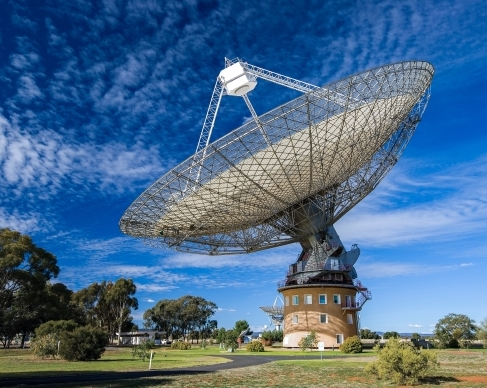
\includegraphics[width=\textwidth]{images/CSIRO-Parkes-Wiradjuri-naming-Murriyang.jpg}
                \caption{\raggedright The 64m telescope (Murriyang) at Parkes Observatory}
                \label{fig:murriyang}
            \end{subfigure}
            \begin{subfigure}{0.45\textwidth}
                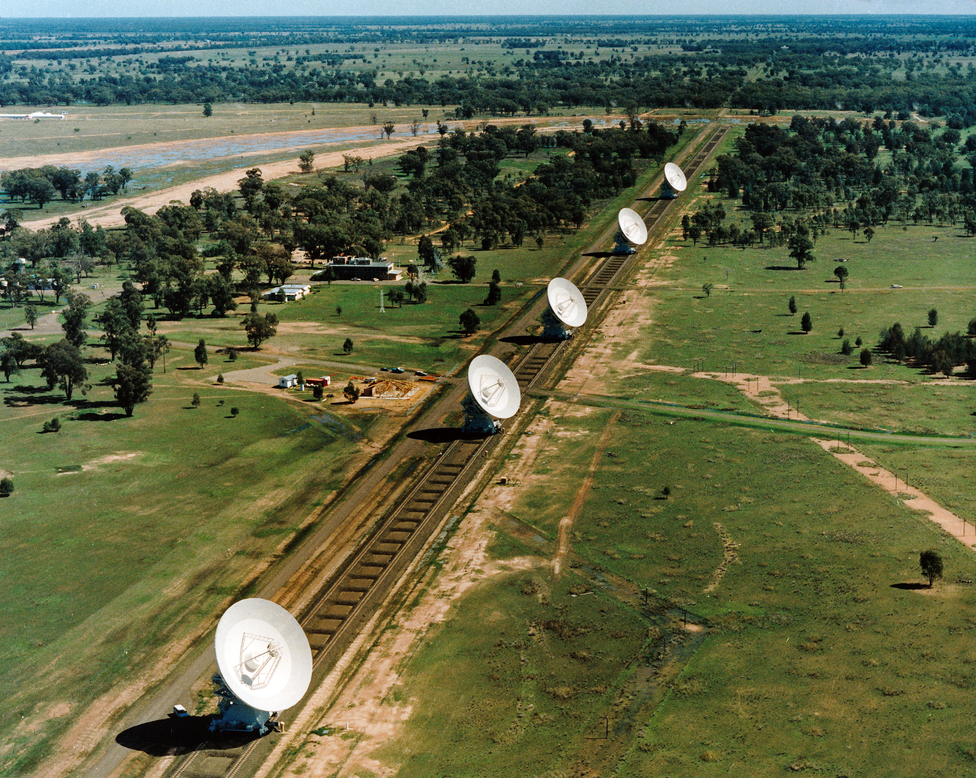
\includegraphics[width=\textwidth]{images/atca.jpg}
                \caption{ATCA near Narrabri\\\phantom{a}}
                \label{fig:atca}
            \end{subfigure}
            \caption[A single dish telescope and a radio array.]{\label{fig:telescopes} (a) A single-dish telescope and (b) an array. Images: CSIRO.}
        \end{figure}

        Radio observations \DIFdelbegin \DIFdel{may be made either with }\DIFdelend \DIFaddbegin \DIFadd{are made with either }\DIFaddend \defn{single-dish telescopes}, like the famous Parkes Radio Telescope (Murriyang), or \defn{radio arrays}, like the Australia Telescope Compact Array (ATCA), both shown in \autoref{fig:telescopes}. Both have their advantages. Single-dish telescopes are able to measure absolute brightnesses (while arrays can only measure relative brightnesses, and must therefore be calibrated to a source of known brightness). Interferometric arrays can achieve incredibly high resolution, as the resolution is inversely proportional to the distance between the most distant array elements (while the resolution of single dish telescopes is inversely proportional to the diameter of the dish).

        Radio telescopes can be thought of as sampling the \defn{$u$-$v$ plane}, the Fourier transform of the sky. The $u$-$v$ plane is perpendicular to the line-of-sight. Each pair of antennae in an array samples two points on this plane, each corresponding to the vector between the antennae projected onto the $u$-$v$ plane, called a \defn{baseline}. Longer baselines therefore correspond to higher (spatial) frequencies, which is why long baselines provide high resolution. Diffuse emission is characterised mainly by low (spatial) frequency components, while compact emission is characterised by a broad range of frequency components\DIFdelbegin \DIFdel{, so }\DIFdelend \DIFaddbegin \DIFadd{. This means that }\DIFaddend large angular scale, diffuse emission both a) takes up less space on the $u$-$v$ plane than compact sources and b) occupies spaces much closer to the origin on the $u$-$v$ plane. Some intuition on this can be obtained by examining the Fourier transform of a 2D Gaussian:
        \begin{equation}
            \mathcal F_{x, y}\left[\frac{1}{2\pi\sigma^2} e^{-(x^2 + y^2) / 2\sigma^2}\right] = e^{-2\sigma^2 \pi^2(u^2 + v^2)}.
        \end{equation}
        From this equation we can see that the Fourier transform of a fairly \emph{compact} Gaussian \DIFaddbegin \DIFadd{(small $\sigma$) }\DIFaddend would be quite broad, taking up many frequencies in the $u$-$v$ plane, while a very \emph{diffuse} Gaussian \DIFaddbegin \DIFadd{(large $\sigma$) }\DIFaddend would have a very narrow Fourier transform. The upshot of this is that long baselines sacrifice sensitivity to diffuse emission for high resolution. Single-dish radio telescopes are unable to make the same tradeoff, as they are only able to sample a disc centred on the origin\footnote{This is, incidentally, why single-dish telescopes can measure the absolute brightness while arrays cannot: \DIFdelbegin \DIFdel{there }\DIFdelend \DIFaddbegin \DIFadd{There }\DIFaddend is no way to measure the origin in the $u$-$v$ plane as there is no way for two array antennae to be infinitely close together (forming a zero-length baseline), and the origin contains the absolute brightness information, much like how the centre of a Fourier transform contains the mean.}. This loss of larger scale diffuse emission is often called \defn{resolving out}. An example of this is shown in \autoref{fig:resolved-out}, where (a) and (b) are the same radio galaxy observed with the same telescope, the Very Large Array, with the only difference being that the VLA was in \DIFaddbegin \DIFadd{the }\DIFaddend B configuration for (a) and the D configuration for (b). The B configuration moves the antennae of the VLA far apart, while the D configuration keeps them close together.

        \begin{figure}
            \centering
            \begin{subfigure}{0.45\textwidth}
                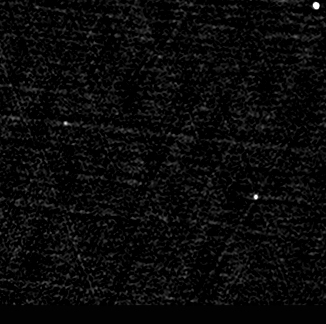
\includegraphics[width=\textwidth]{images/im-contours.jpg}
                \caption{FIRST}
                \label{fig:im-contours-first}
            \end{subfigure}
            \begin{subfigure}{0.45\textwidth}
                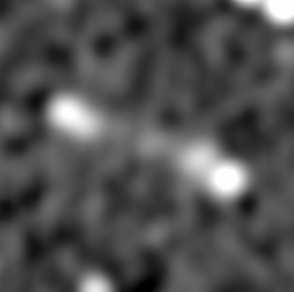
\includegraphics[width=\textwidth]{images/im-contours-2.jpg}
                \caption{NVSS}
                \label{fig:im-contours-nvss}
            \end{subfigure}
            \caption[An example of a `resolved out' radio galaxy.]{\label{fig:resolved-out} A fairly diffuse FRII, J0016+0420, observed with the VLA in the (a) FIRST \citep{becker95first} and (b) NVSS \citep{condon98nvss} surveys. \citep[GRG1 from ][]{dabhade_discovery_2017}}
        \end{figure}

    \subsection{Methods of aggregation}
    \label{sec:methods-aggregation}

        Most large radio catalogues are of \emph{components} rather than sources, most likely because manual methods remain the best way to aggregate components into sources. Many component catalogues have source catalogues of some interesting subset later derived from them by manual inspection \citep[e.g.][]{dabhade_discovery_2017}. Such manual searches are often assisted by automated methods \citep[e.g.][]{proctor_morphological_2011}. The Radio Galaxy Zoo citizen science project has also, with the help of over 10~000 volunteers, aggregated over 75~000 sources from FIRST (Wong et al. in prep\DIFaddbegin \DIFadd{.}\DIFaddend ) and ATLAS \citep{banfield15}, which is one of the largest (if not the largest) extant catalogues of manually aggregated sources.

        Automated methods have been developing steadily as data volumes \DIFdelbegin \DIFdel{have grown}\DIFdelend \DIFaddbegin \DIFadd{grow}\DIFaddend . A Bayesian approach, fitting models of sources to component locations, was introduced by \citet{fan15} and later expanded upon \citep{fan_optimal_2020}. Machine learning methods have also become increasingly popular. \citet{proctor_selection_2016} aggregated radio components using a decision tree classifier and used the results to search for giant radio galaxies \citep[see also][]{proctor_morphological_2011,proctor06}. \citet{wu19claran} applied a deep learning model to identify radio sources from an image of radio components, training this model on the Radio Galaxy Zoo FIRST dataset. Most recently \citet{galvin_cataloguing_2020} used a nested self-organising map, a kind of neural network, to cluster similar sources and then aggregated them into sources using manual labelling of the clusters and some heuristics.

        Any method for cross-identification of components can also be used to aggregate components. Cross-identify all components with their host galaxies, then components that share a host are almost always part of the same radio source. It is this approach \DIFaddbegin \DIFadd{that }\DIFaddend we will later take to aggregating sources in \autoref{cha:rlfs}. There is no obvious inverse algorithm (to go from aggregate sources to cross-identifications) although some algorithms attempt to solve both problems simultaneously \citep{fan_optimal_2020,fan15}.


\section{Summary: radio sources}
\label{sec:summary-radio}

    The radio sky is vibrant and exciting, and current and new wide-area radio surveys are opening up new avenues of exploring this space. In this chapter we introduced radio sources that you might see in the radio sky, including the often-extended AGN. We discussed their radio emission and emission mechanisms, and described some aspects of their morphology and structure. We also looked at ways that radio sources can be classified, aggregated, and cross-identified with their counterparts at other wavelengths. In the next chapter, we will introduce machine learning concepts that we will use to develop methods for exploiting the vast amount of data \DIFaddbegin \DIFadd{that }\DIFaddend radio telescopes provide on radio sources.

    % \begin{itemize}
    %     \item machine learning in astronomy and radio astronomy (literature review)
    %     \item summarising the basics of machine learning (later sections of course complicate these): \begin{itemize}
    %         \item predictors
    %         \item features
    %         \item labels
    %         \item optimisation
    %         \item data
    %         \item expertise
    %     \end{itemize}
    %     \item specific predictors
    %     \item features: \begin{itemize}
    %         \item feature selection and design, and the benefit of domain knowledge
    %         \item feature extraction
    %         \item neural networks
    %     \end{itemize}
    %     \item labels: \begin{itemize}
    %         \item training labels and testing labels
    %         \item where do labels come from? domain experts, crowdsourcing, citizen science, simulations...
    %         \item label noise and unreliable annotators
    %         \item multiple unreliable annotators
    %     \end{itemize}
    %     \item citizen science: \begin{itemize}
    %         \item citizen science in astronomy
    %         \item designing good citizen science
    %         \item benefits and challenges of citizen science
    %         \item challenges in ML on crowdsourcing/citizen science
    %         \item rant about how citizen science is different to crowdsourcing from an ML perspective
    %     \end{itemize}
    % \end{itemize}

% Here we need to talk about the fundamentals of machine learning. We'll start with problem formulations and what machine learning is, then discuss terminology and classification. We need to cover the difficulties of labels and the lack of groundtruth in astronomy, the problem and handling of uncertainties, and feature selection. We also need to talk about the importance (or unimportance?) of interpretability and how this ties into astronomy, and the unique idea of using machine learning as a pathway to understand something important about physics.
%!tex root=./thesis.tex
\chapter{Machine Learning for Astroinformatics}
\label{cha:background-ml}

Machine learning was once described to me by an anonymous supervisor as ``the statistics kept at the back of the textbook''. But even accepting its grounding in statistics, is this really an accurate description of the field? I think of machine learning as a \DIFaddbegin \DIFadd{combination of three pieces: a }\DIFaddend data-driven way of formalising predictive problems\DIFdelbegin \DIFdel{and }\DIFdelend \DIFaddbegin \DIFadd{, a way of }\DIFaddend converting between different kinds of statistical problems, \DIFdelbegin \DIFdel{as well as an accompanying }\DIFdelend \DIFaddbegin \DIFadd{and a }\DIFaddend set of methods and practices for handling data and uncertainty. The eventual goal is to design some method or algorithm that automatically discovers useful patterns in (potentially very large) \DIFdelbegin \DIFdel{data sets}\DIFdelend \DIFaddbegin \DIFadd{datasets}\DIFaddend . There are three core components of machine learning: the data, the model, and learning \citep{deisenroth_mathematics_2020}. Before discussing these, we will look at the kinds of problems that machine learning solves.

\section{Prediction}

    Machine learning aims to solve \defn{prediction tasks}: problems where we have some data and we seek some kind of output based on that data. Central to prediction tasks are predictors, the objects we train based on data.

    \subsection{Predictors}
    \label{sec:predictors}
        A \defn{predictor} is an object that makes predictions based on an input. A predictor can be a function or a probabilistic model, depending on the machine learning approach being undertaken.

        As a function, a predictor maps from some input domain $\mathcal X$ into some output domain $\mathcal Y$, and is usually written as
        \begin{equation}
            f : \mathcal X \to \mathcal Y.
        \end{equation}
        $\mathcal X$ and $\mathcal Y$ are commonly (but certainly not always) a real vector space $\mathbb R^n$. Because the goal of machine learning involves \emph{finding} a suitable function $f$ for the task at hand, the set of functions is usually constrained. For example, if $\mathcal X = \mathbb{R}^n$, we might require that $f$ is a linear function $\mathbb R^n \to \mathbb R$, easily parametrised by $n + 1$ constants. This constraint is called a \defn{model}. Models are often (but not always) parametrised and training the model refers to finding a good set of parameters. The parameters are sometimes called \defn{weights}. To avoid ambiguity, parameters of the model that are not changed during training are called \defn{hyperparameters} and may include regularisation terms, constraints, or variations of the model.

        Some predictors can be described as a probabilistic model. In this case a predictor is a joint probability distribution between observations and hidden parameters \citep{deisenroth_mathematics_2020}. Using a probabilistic predictor allows us to formally describe and work with uncertainty both in the input space and output space. Such a predictor is usually parametrised by a finite set of parameters, which already includes most common probability distributions.

        We \DIFdelbegin \DIFdel{will }\DIFdelend generally assume that our data are generated from some unobserved, true function called the \defn{groundtruth}. This might be a physical process, or a complicated sampling function from some unknown vector space. The assumptions we make on this generative function can greatly change the way we approach machine learning problems.

        In some sense, the goal of machine learning is to identify a good predictor from within the space of all possible predictors. Of course, this begs the question: \DIFdelbegin \DIFdel{what }\DIFdelend \DIFaddbegin \DIFadd{What }\DIFaddend is a `good' predictor? We will return to this when we discuss learning, but for now, a good predictor is one that approximates the groundtruth well.

    \subsection{Classification}
    \label{sec:classification}

        \defn{Classification} is the machine learning task of predicting discrete, unstructured values \citep{deisenroth_mathematics_2020}. These values are called \defn{classes}. Classification is arguably the most important prediction task, as many other problems can be formalised as classification. Astronomy has its fair share of classification tasks, from classical astronomy tasks like galaxy morphology classification \citep[appearing in machine learning literature as e.g.][]{dieleman15cnn} to transient detection \citep[e.g.][]{scalzo_skymapper_2017}; see \autoref{sec:classification-of-agn} for more examples.

        A classification problem seeks a predictor where $\mathcal Y$ represents a finite, discrete set of classes. Classification tasks are usually delineated by the number of classes: \DIFdelbegin \DIFdel{there }\DIFdelend \DIFaddbegin \DIFadd{There }\DIFaddend are either two classes or more than two classes. The former are called \defn{binary classification} tasks and the latter are \defn{multiclass classification} tasks. The reason for this split is that binary classes are dramatically easier to reason about and analyse, and many special cases exist for binary where they do not for multiclass.

        $\mathcal Y$ for a binary task is usually represented as $\mathcal Y = \{0, 1\}$. $1$ is called the \defn{positive class}; $0$ is called the \defn{negative class}.

        An easy way to see why many tasks can be formalised as classification can be found by taking any prediction problem $\mathcal X \to \mathcal Y$ and reinterpreting it as the binary classification problem $\mathcal X \times \mathcal Y \to \{0, 1\}$, i.e. instead of taking an input and predicting an output, take an input and a potential output and determine if they should be related. Of course this is not always the most efficient way to solve a prediction problem but the many known properties of classification make it an appealing framework to cast problems into. In \autoref{cha:cross-id}, we will cast the radio astronomy problem of cross-matching galaxies seen in different wavelengths into a binary classification problem, and in \autoref{cha:faraday} we will classify radio observations as Faraday complex or Faraday simple.

        There are three different formalisms for the output of a binary classifier. The output may be a \defn{score}, a \defn{class probability estimate}, or a \defn{predicted class}. A predicted class is what first comes to mind as a representation of binary classes: \DIFdelbegin \DIFdel{the }\DIFdelend \DIFaddbegin \DIFadd{The }\DIFaddend classifier outputs either 0 or 1, with no way of representing ambiguity. A class probability estimate is a number from 0 to 1 which represents the probability that an example is in the positive class, i.e. if $f$ is a classifier then $f(x) = p(y = 1 \mid x)$. Class probability estimates may be output by probabilistic classifiers, or may be estimated from non-probabilistic classifiers. Finally, a score is a value that tends to be larger for elements of the positive class, with less ambiguous examples being given a higher score. Scores are often converted into class probability estimates by applying a sigmoid (see \autoref{sec:logistic-regression}). There are multiple ways to generalise these concepts to multiclass classification. Having a score or a class probability estimate can be more useful than only having a predicted class. For example, you could sort your examples by how likely they are to be a member of the positive class. This underpins our approach to casting cross-identification as binary classification in \autoref{cha:cross-id}.

    \subsection{Regression}
    \label{sec:regression}

        The other main kind of supervised prediction task is \defn{regression}, which is the machine learning task of predicting ordered (and usually continuous) values. In a regression problem, we seek a predictor where $\mathcal Y$ is a set of ordered values, usually a subset of $\mathbb R^k$ for some positive natural $k$. Regression is ubiquitous in astronomy, from simple linear relationships like the famous Tully-Fisher relation \citep{tully_new_1977} to estimation of redshifts from photometric observations \citep[called \defn{photometric redshifts}; first introduced by][]{baum_photoelectric_1962}. \DIFdelbegin \DIFdel{We will }\DIFdelend \DIFaddbegin \DIFadd{This thesis does }\DIFaddend not directly address any regression problems\DIFdelbegin \DIFdel{in this thesis, but we will }\DIFdelend \DIFaddbegin \DIFadd{, but does }\DIFaddend make use of their results.

\section{Data and representation}
\label{sec:data-and-representation}

    Machine learning is centred on data and the extraction of useful information from that data. Data can include anything from numeric information, documents, or images, to spectra or galaxies. A collection of data is called a \defn{dataset} and an element of this dataset is (interchangably) called an \defn{example} or \defn{instance}. Generally, data are not easy to work with in their original form and must be converted into a numerical representation before use. We usually convert our data into real vectors in $\mathbb R^n$ as it is relatively easy to work with both numerically and analytically. Each axis of this vector space is called a \defn{feature} and the space as a whole is called the \defn{feature space}. Features are non-trivial to choose, and finding good features often requires the expertise of a human who is well-versed in the original dataset (a \defn{domain expert}). The process of finding features is called \defn{feature selection}, \defn{feature design}, or \defn{feature engineering}.

    What makes a feature good? Intuitively, we want to transform our data into a space where it is easy to work with: a space where properties we care about are obvious, easy to extract, behave nicely, and work well with our model. For this reason, features will vary tremendously depending on the problem being faced, and the same data may be represented in many different ways. Much of early machine learning literature focused on finding good methods to automatically develop features (generally called \defn{feature extraction}), and much early applied machine learning focused on identifying these features manually so that good predictors could be easily found. An astronomical example is \citet{proctor06}, who developed features for representing radio galaxies for the purpose of sorting them. State-of-the-art models like deep neural networks \citep[e.g.][]{dieleman15cnn} can be viewed as developing their own task-specific features as part of their training (see \autoref{sec:cnns}). These deep learning features can be useful (e.g. when it is hard or slow to define good features manually), but are usually hard to interpret. A good feature space \DIFdelbegin \DIFdel{will have }\DIFdelend \DIFaddbegin \DIFadd{has }\DIFaddend a structure that reflects the components of the intrinsic structure of the input data which are useful for the prediction task at hand. Good features may also be useful in other related tasks, such as dataset exploration, dataset visualisation, or other prediction tasks. \autoref{cha:faraday} largely focuses on finding good features for identifying Faraday complexity in polarised sources.

    \defn{Labels} comprise another very important piece of the machine learning puzzle. Training a predictor with supervised learning requires some known pairs of inputs and outputs, and the known outputs are called labels. Like features, labels also need to be encoded in some way, and this depends on the specific task. Much like features, we want to embed the labels into a space which is easy to work with and has a meaningful structure. For problems where we know the outputs we wish to obtain, this can be a lot simpler than feature selection. For example, a binary classification problem \DIFdelbegin \DIFdel{will have }\DIFdelend \DIFaddbegin \DIFadd{has }\DIFaddend only two possible outputs. Common representations for \DIFdelbegin \DIFdel{this would be }\DIFdelend \DIFaddbegin \DIFadd{these are }\DIFaddend $\{0, 1\}$ as described in \autoref{sec:classification}, but we could also represent the labels as $\{[1, 0]^T, [0, 1]^T\}$, called a \defn{one-hot encoding}. The advantage of the former is its simplicity and ease of integration into binary classification equations, but the advantage of the latter is that it is easily extended into multiclass classification without imposing order on the classes. Despite being simpler to encode, labels can carry a lot more difficulty than features due to their comparative rarity: \DIFdelbegin \DIFdel{in }\DIFdelend \DIFaddbegin \DIFadd{In }\DIFaddend essence, features are cheap and labels are expensive. We will discuss labels in more detail in \autoref{sec:labels}.

\section{Loss functions}
\label{sec:training}

    \defn{Training} a model is the process of using data to find a good predictor that fits the model's constraints. This is generally achieved by minimising a \defn{loss} (also called \defn{error} or \defn{cost}) function over the model.

    Put simply, a loss function is a function of a predictor and a dataset which is chosen to be a proxy for how good the predictor is at predicting that dataset. We try to choose loss functions that are high-valued for a predictor that poorly describes the dataset, and are low-valued for a predictor that well-describes the dataset. Sometimes (and in both cases listed in this section) the loss is minimised at zero, when the predictor perfectly captures the dataset (though whether this is possible, or whether this is even a desired result, is another question).

    What should the loss function be for a given problem? The answer is not always obvious. Take for example a binary classification problem. The ``obvious'' loss would be the complement of the accuracy: the rate at which the predictor incorrectly guesses the label. This is easy to compute and we would like our predictor to have a high accuracy. But this is not a good choice: \DIFdelbegin \DIFdel{it }\DIFdelend \DIFaddbegin \DIFadd{It }\DIFaddend is tremendously hard to work with as it takes on discrete values, because the accuracy is the number of correct predictions divided by the total number of examples. It is hard to motivate with probabilistic arguments. Finally, it is unclear how the accuracy should work in the case of a probabilistic model.

    Instead, the loss function is usually derived by making assumptions on the structure of the data and task. The main assumption we usually make is that data are drawn \defn{independently and identically distributed} (IID), that is, each example is drawn from the same distribution and is not dependent on any other examples. We also assume a structure of the noise in the observed labels: \DIFdelbegin \DIFdel{training }\DIFdelend \DIFaddbegin \DIFadd{Training }\DIFaddend data are almost never completely accurate, \DIFdelbegin \DIFdel{and so there will be }\DIFdelend \DIFaddbegin \DIFadd{so there is usually }\DIFaddend intrinsic noise in the distribution of labels about their unobserved ``true'' value. To demonstrate these assumptions, we will now derive loss functions for regression and binary classification. The loss function we derive depends on the model we assume for the noise; for example, assuming Gaussian noise gives us the common least-squares loss.

        \subsection{Loss function for regression}
        \label{sec:loss-regression}

            To derive a loss function for regression, let us assume that our labels are a random variable $y$ modelled by a predictor $y = f(x)$. Further, let us assume that a predicted $y$ is normally distributed about its true value, i.e.
            \begin{equation}
                y \sim \mathcal N(\mu, \sigma^2)
            \end{equation}
            for the true mean $\mu$ and standard deviation $\sigma$ where $\mathcal N$ is the normal distribution:
            \begin{equation}
                \mathcal N(a \mid \mu, \sigma^2) = \frac{1}{\sqrt{2\pi\sigma^2}} e^{-\frac{(a - \mu)^2}{2\sigma^2}}.
            \end{equation}
            Under this assumption the probability that $y$ is equal to a target $t$ given an example $x$ is
            \begin{equation}
                p(y = t \mid x) = \mathcal N(t \mid f(x), \sigma^2).
            \end{equation}

            What would the probability be of observing a set of targets $T = \{t_1, \dots, t_n\}$ given corresponding examples $X = \{x_1, \dots, x_n\}$? Letting $Y = \{y_1, \dots, y_n\}$ be random variables like $y$, the joint probability distribution $p(Y = T \mid X)$ is
            \begin{equation}
                p(Y = T \mid X) = \prod_{i = 1}^n p(y_i = t_i \mid x_i)
            \end{equation}
            by using our independence assumption. We can then substitute the normal distribution:
            \begin{equation}
                p(Y = T \mid X) = \prod_{i = 1}^n \mathcal N(t_i \mid f(x_i), \sigma^2).
            \end{equation}
            $p(Y \mid X)$ is called the \defn{likelihood}. We would like to maximise this likelihood over $f$, which is called a \defn{maximum likelihood} approach to finding a predictor. It is, however, not very easy to work with in this current form. Maximising the likelihood is equivalent to minimising its negative logarithm, so we write:
            \begin{equation}
                \mathcal L(f; T, X) = -\sum_{i = 1}^n \log \mathcal N(t_i \mid f(x_i), \sigma^2)
            \end{equation}
            where $\mathcal L$ is the \defn{negative log-likelihood}, a loss function. We can simplify this dramatically by cancelling the logarithm and the exponential within the normal distribution:
            \begin{equation}
                \mathcal L(f; T, X) = \sum_{i = 1}^n \frac{(t_i - f(x_i))^2}{2\sigma^2}
            \end{equation}
        and by noting that arbitrary scaling of $\mathcal L$ does not change the minimising $f$ we can scale $\mathcal L$ by $\sigma^2$ and arrive at the \defn{sum-of-squares error}, also known as the \defn{least-squares error}, the most common loss function for regression:
            \begin{equation}
                \mathcal L(f; T, X) = \frac{1}{2} \sum_{i = 1}^n (t_i - f(x_i))^2.
            \end{equation}
            The factor of half helps keep the derivative tidy:
            \begin{equation}
                \frac{\mathrm{d}\mathcal L}{\mathrm{d}\theta}(f; T, X) = \sum_{i = 1}^n (t_i - f(x_i)) \frac{\mathrm{d}f}{\mathrm{d}\theta}(x_i).
            \end{equation}

        \subsection{Loss function for binary classification}
        \label{sec:loss-classification}

            Now we will calculate a loss function for binary classification. As for regression, we first assume a form for the noise. Assume that our labels are a random variable $y \in \{0, 1\}$ and that the prediction $y$ is drawn from a Bernoulli distribution based on a predictor $f(x)$:
            \begin{equation}
                p(y = t \mid x) = \mathcal B(t; f(x)).
            \end{equation}

            The Bernoulli distribution is parametrised by one parameter, usually called $p \in (0, 1)$, and in this case set to $f(x)$. It is:
            \begin{equation}
                \mathcal B(a; p) = p^a(1 - p)^{1 - a}.
            \end{equation}
            It can be thought of as a biased coin toss with a probability $p$ of tossing heads. To gain some intuition into how this expression works, imagine setting $a$ to 0 and then to 1. Continuing to derive the loss function, we once again determine the likelihood making the IID assumption:
            \begin{equation}
                p(Y = T \mid X) = \prod_{i = 1}^n p(y_i = t_i \mid x_i) = \prod_{i = 1}^n f(x_i)^{t_i}(1 - f(x_i))^{1 - {t_i}}.
            \end{equation}
            Then we find the negative log-likelihood and hence what is known as the \defn{binary cross-entropy loss} for binary classification:
            \begin{align}
                \mathcal L(f; T, X) &= -\sum_{i = 1}^n \log \left(f(x_i)^{t_i}(1 - f(x_i))^{1 - {t_i}}\right)\\
                    &= -\sum_{i = 1}^n t_i \log f(x_i) + (1 - t_i) \log (1 - f(x_i)).
            \end{align}

            This is the standard loss used for logistic regression (\autoref{sec:logistic-regression}).

            % \begin{equation}
            %     \frac{\mathrm{d}\mathcal L}{\mathrm{d}\theta}(f; T, X) = \sum_{i = 1}^n -\frac{1 - t_i}{1 - f(x_i)} \log (1 - f(x_i)) + t_i \log f(x_i).
            % \end{equation}

    \subsection{Gradient descent}
    \label{sec:gradient-descent}

        Given a loss function and a parametrised model, how can we find parameters for the model that minimise the loss function? There are many optimisation strategies but if both the loss function and model are differentiable with respect to the parameters then we can employ a particularly efficient approach: \defn{gradient descent}. Assume we have a model $f(x; \vec w)$ parametrised by some vector $\vec w$ and a loss function $\mathcal L(\vec w; T, X)$. Then the value of $\vec w$ after the $k + 1$th update of gradient descent is
        \begin{equation}
            \label{eq:gradient-descent}
            \vec w^{(k + 1)} = \vec w^{(k)} - \lambda \nabla_{\vec w} \mathcal L(\vec w^{(t)}; T, X)
        \end{equation}
        where $\lambda > 0$ is a small scalar called the \defn{learning rate}. With an appropriately small choice of $\lambda$ $\vec w$ will converge to a local minimum of $\mathcal L$. Many variations on this concept exist which attempt to avoid local minima, such as introducing a `momentum' term that accumulates as multiple iterations move $\vec w$ in the same direction. If the loss function is convex, then any minimum is the global minimum (there are no local minima).

\section{Models}
\label{sec:models}

    This section describes some common models for classification. There are a plethora of different classification models and variations on these models, but I will present here only those relevant to this thesis: logistic regression, decision tree ensembles, and neural networks. These are, not coincidentally, also the most common models in astroinformatics. Logistic regression provides reliable and interpretable results. Decision tree ensembles are a fantastic off-the-shelf choice which work on a large variety of datasets. Neural networks have \DIFdelbegin \DIFdel{proved }\DIFdelend \DIFaddbegin \DIFadd{proven }\DIFaddend extremely effective for a wide variety of tasks, especially in computer vision.

    \subsection{Logistic regression}
    \label{sec:logistic-regression}

        \defn{Logistic regression} is a linear, binary, probabilistic classifier. Linear classifiers can only separate classes using a hyperplane in the feature space, with objects on one side of the plane being assigned to one class and objects on the other side being assigned to the other. A binary classifier works on binary classification tasks. Probabilistic classifiers, as discussed in \autoref{sec:classification}, have outputs interpretable as class probabilities.

        Logistic regression in a $d$-dimensional feature space is parametrised by a \defn{weights vector} $w \in \mathbb R^d$. Given a set of features $x \in \mathbb R^d$, logistic regression is:
        \begin{equation}
            \label{eq:logistic-regression}
            f(x; w) = \sigma(w^T x)
        \end{equation}
        where $\sigma$ is the \defn{logistic function} or \defn{sigmoid}, which is a monotonic and bijective function:
        \begin{equation}
            \label{eq:logistic-function}
            \sigma(a) = \frac{1}{1 + e^{-a}}.
        \end{equation}
        The output of logistic regression applied to an example $x$ is the probability that $x$ is in the positive class. $\sigma$, and thus logistic regression, has a domain of $(-\infty, \infty)$ and a range of $(0, 1)$. This enforces the output to be like a probability. $w^T x= 0$ defines a $d$-dimensional hyperplane, called the \defn{separating hyperplane} or \defn{decision surface}. Logistic regression is differentiable, which allows us to optimise its parameters $w$ using gradient descent. Interpreting the classifier is possible through examining the weights vector, with a larger absolute value of a weight corresponding to a `more important' feature. The weights from logistic regression can be used to produce scores or class probability estimates (\autoref{sec:classification}): $w^T x$ is a score, $\sigma(x^T x)$ is a class probability estimate, and thresholding either the score or the class probability estimate at $0$ gives a discrete class.

        A limitation of logistic regression is its sensitivity to scale. Features need to be of approximately the same order of magnitude and should have a standard deviation of approximately 1. An implicit assumption is that each \DIFdelbegin \DIFdel{features }\DIFdelend \DIFaddbegin \DIFadd{feature }\DIFaddend has a mean of 0 across the dataset. This can be enforced by normalising and scaling: subtract the mean of the dataset and divide by the new standard deviation.

        We apply logistic regression to binary classification problems in \autoref{cha:cross-id} and \autoref{cha:faraday}.

    \subsection{Decision tree ensembles}
    \label{sec:decision-trees}

        A \defn{decision tree} is a non-linear classifier. It repeatedly splits a dataset based on binary comparisons until every subset contains only one class (or mostly one class, with the amount of purity left as a hyperparameter). Each split only uses one feature for the comparison, making decision trees relatively easy to visualise and interpret. However, because of this, each split is axis-parallel, which can be a limitation for some datasets. They are not sensitive to scale and do not require a zero mean, making them easy to apply without preprocessing a dataset.

        Key limitations of a decision tree are:
        \begin{itemize}
            \item They can only output a prediction, not a confidence of this prediction or a score of how likely an instance is to be found within each class.
            \item Small changes to the dataset or training method can result in large changes to the tree.
            \item They tend toward overfitting the training set.
            \item With many low-information features, decision trees have quite poor performance \citep{breiman01random-forest}.
        \end{itemize}

        A \defn{decision tree ensemble} aims to reduce some of these limitations by training multiple, slightly different, independently-trained decision trees. Depending on the implementation each constituent decision tree may only have access to some of the features or some of the data. To predict, each tree produces a prediction and `votes' for this prediction; the votes \DIFdelbegin \DIFdel{can be }\DIFdelend \DIFaddbegin \DIFadd{are }\DIFaddend combined to produce the overall prediction (e.g. with majority voting). A simple example of such an ensemble is decision tree bagging \citep{breiman_bagging_1996}, which trains each tree with a random subset of the training data and takes a plurality vote. Decision tree ensembles decrease variance, increase the usability of low-information features, and increase stability of the trained model \citep{breiman01random-forest}. Averaging over the classifications produced by each tree gives a number that can be interpreted as a class probability estimate.

        The most well-known description of decision tree ensembles is the \defn{random forest} \citep{breiman01random-forest}, which has found common use in astronomy partly to its readily available \texttt{Python} implementation in \texttt{scikit-learn} \citep{pedregosa11sklearn}. Splits are decided from a subset of features and training samples are randomly drawn with replacement from the total training set. One downside of random forests is the large number of hyperparameters that need to be set, and these vary a lot depending on the problem being addressed.

        We apply decision tree ensembles to binary classification problems in \autoref{cha:cross-id} and \autoref{cha:faraday}.

    \subsection{Convolutional neural networks}
    \label{sec:cnns}

        A \defn{neural network} is a directed graph of transformations, each node representing a transformation that linearly combines its inputs and applies a non-linear function called the \defn{activation function} to the result. The inputs to the graph are the features. A particularly prominent kind of neural network is the \defn{fully-connected neural network}, where nodes are arranged into layers, with each node in a layer taking as input every output from the previous layer. Each layer can then be represented by a matrix multiplication of the outputs of the previous layer by a weight matrix, composed with the activation function. Fully-connected $K$-layer neural networks have the form:
        \begin{align}
            f(x; W_K, \dots, W_1) &= h_K(x; W_K, \dots, W_1)\\
            h_i(x; W_i, \dots, W_1) &= a(W_i h_{i - 1}(x; W_{i - 1}, \dots, W_1))\label{eq:hidden-layer}\\
            h_1(x; W_1) &= a(W_1 x)
        \end{align}
        where $a$ is the activation function. $h_i$ are called \defn{hidden layers}. In fact, neural networks are usually described by their layer structure rather than graph structure, with the addition of `concatenation layers' to combine outputs from previous layers. Neural networks may be used for regression or for classification; these are structured the same but for classification the last activation function is replaced by sigmoid (for binary classification) or its multiclass counterpart softmax.

        \defn{Convolutional neural networks} \citep[CNN;][]{lecun98} are \DIFdelbegin \DIFdel{a variant }\DIFdelend \DIFaddbegin \DIFadd{variants }\DIFaddend of neural networks that are particularly well-suited to inputs that have local structure, such as images or spectra. Layers in the network may be \defn{dense layers} of the same form as \autoref{eq:hidden-layer}, or \defn{convolutional layers}, where the weights are convolved with the input rather than multiplied. These convolutional weights are called \defn{filters} and they are small compared to the dimensionality of the input. CNNs are translation-invariant \citep{waibel_phoneme_1989} and derive features from local relationships thanks to the trainable filters.

        We apply CNNs to binary classification problems in \autoref{cha:cross-id} and \autoref{cha:rlfs}, and compare our results to a state-of-the-art CNN in \autoref{cha:faraday}.

\section{Labels}
\label{sec:labels}

    As described in \autoref{sec:data-and-representation}, labels are the known outputs of supervised prediction tasks. They are used for two main, distinct purposes: training and validation. Labels for training are used to evaluate loss and determine how to update the model. Labels for validation are used to evaluate and characterise the model's behaviour.

    \subsection{Where do labels come from?}
    \label{sec:sources-of-labels}

        We previously said that labels were `expensive'. This is to be interpreted as expensive in either or both time and money: \DIFdelbegin \DIFdel{labelling }\DIFdelend \DIFaddbegin \DIFadd{Labelling }\DIFaddend can be a slow, manual\DIFdelbegin \DIFdel{process, and labelling can be costly. Labelling }\DIFdelend \DIFaddbegin \DIFadd{, and process. It }\DIFaddend is usually completed by hand, manually examining instances and determining \DIFdelbegin \DIFdel{what }\DIFdelend \DIFaddbegin \DIFadd{which }\DIFaddend class they belong to (for classification) or what target they ought to be associated with (for regression). In astronomy this usually amounts to expert astronomers examining imagery at multiple wavelengths and making an educated guess as to what the true label \DIFdelbegin \DIFdel{should be}\DIFdelend \DIFaddbegin \DIFadd{is}\DIFaddend , but labelling may also involve follow-up observations (perhaps at higher resolution, greater sensitivity, or at a different wavelength).

        An increasingly popular option for labelling large amounts of data is \defn{citizen science}: asking volunteers who are interested in contributing to science to label our data. Citizen science projects can be a fantastic opportunity for both science and outreach. For example, the ABC's `Stargazing Live' television programme engaged viewers and with their help found four exoplanets in just 48 hours \citep{miller_stargazing_2017} and labelled 120~000 SkyMapper images\footnote{Citizen scientists actually produced around 5 million labels---these were aggregated to 120~000 to reduce noise.} in just three days \citep{tucker_stargazing_2017}. The downside of citizen science is that non-expert labellers may be less accurate than experts, and indeed some may even be malicious and provide intentionally incorrect labels \citep{zhang_learning_2016}.

        Astronomers often face a large collection of unlabelled data and must choose which to label. Choosing what to label is a broad topic of research separately in machine learning \citep[often called active learning e.g.][]{gilyazev_active_2018}, in astronomy (`follow-up observations'), and in citizen science project design \citep[e.g. citizen science project Snapshot Serengeti found that showing volunteers \emph{uninteresting} images helped retain engagement;][]{sieland_snapshot_2015}.

    \subsection{Label noise}
    \label{sec:label-noise}

        \defn{Label noise} is the presence of incorrect labels in the training or validation data set. In classical machine learning there is no such thing: \DIFdelbegin \DIFdel{labels }\DIFdelend \DIFaddbegin \DIFadd{Labels }\DIFaddend are assumed to come from some always-correct `oracle'. In reality, though, labels can be wrong. There is intrinsic noise in data, and even expert astronomers \DIFdelbegin \DIFdel{can }\DIFdelend \DIFaddbegin \DIFadd{may }\DIFaddend disagree on labels due to ambiguities \citep[e.g. around 10 per cent of Radio Galaxy Zoo is extremely divisive amongst expert labellers;][]{banfield15}. All is not lost for machine learning: \DIFdelbegin \DIFdel{many }\DIFdelend \DIFaddbegin \DIFadd{Many }\DIFaddend optimisation targets are robust to label noise \citep{menon15cpe}. One way to think about this is that the loss function for machine learning `smooths over' or `averages out' the noise.

        It is important to note that label noise affects training and validation differently. While it is perfectly possible to train a good model with noisy labels, performance measures are not as robust to label noise. Noise in the validation set can change the reported performance in unpredictable ways and wherever possible should be avoided.


\section{Summary: machine learning}
\label{sec:summary-ml}

    Machine learning is a field of study concerned with ways of automatically finding useful patterns in large datasets, formalising predictive problems, converting between different statistical problems, and handling data and uncertainty. With the large volumes of data radio astronomy faces in the lead-up to the SKA, machine learning provides an avenue for enabling scientific discovery at scale. In this chapter we introduced key concepts of machine learning, including predictors, features, labels, and loss functions. We also highlighted classification tasks as a key kind of prediction problem that we will use to frame astronomical questions throughout this thesis and introduced three classification models: logistic regression, decision tree ensembles, and CNNs. In the next chapter, we will frame the astronomical problem of cross-identification as binary classification, allowing us to train a cross-identification algorithm using an existing catalogue of cross-identifications and hopefully allowing us to cross-identify radio sources en masse.

%!tex root=./thesis.tex
\chapter{Radio Cross-identification}
\label{cha:cross-id}

    % a. introduction and motivation
    % b. binary cross-identification
    % c. crowdsourced data and radio galaxy zoo
    % d. results (from ATLAS and FIRST)
    % e. basically the entire ATLAS paper

This chapter is based on my paper \emph{Radio Galaxy Zoo: Machine learning for radio source host galaxy cross-identification}, by M. J. Alger, J. K. Banfield, C. S. Ong, L. Rudnick, O. I. Wong, C. Wolf, H. Andernach, R. P. Norris, and S. S. Shabala; published in the \emph{Monthly Notices of the Royal Astronomical Society} in 2018. Some minor changes have been made to match the rest of this thesis.\\

In this chapter, we consider the problem of determining the host galaxies of radio sources by cross-identification. This has traditionally been done manually, which will be intractable for upcoming and ongoing wide-area radio surveys like the Evolutionary Map of the Universe (EMU). {Automated cross-identification will be critical for these future surveys, and machine learning may provide the tools to develop such methods.
\DIFaddbegin 

\DIFaddend We applied a standard approach from computer vision to cross-identification, introducing one possible way of automating this problem, and explored the pros and cons of this approach}. We applied our method to the $1.4$~GHz Australian Telescope Large Area Survey (ATLAS) observations of the \emph{Chandra} Deep Field South (CDFS) and the ESO Large Area ISO Survey South 1 (ELAIS-S1) fields by cross-identifying them with the \emph{Spitzer} Wide-area Infrared Extragalactic (SWIRE) survey. We trained our method with two sets of data: expert cross-identifications of CDFS from the initial ATLAS data release and crowdsourced cross-identifications of CDFS from Radio Galaxy Zoo. {We found that a simple strategy of cross-identifying a radio component with the nearest galaxy performs comparably to our more complex methods, though our estimated best-case performance is near 100 per cent. ATLAS contains 87 complex radio sources that have been cross-identified by experts, so there are not enough complex examples to learn how to cross-identify them accurately. Much larger datasets are therefore required for training methods like ours. We also showed that training our method on Radio Galaxy Zoo cross-identifications gives comparable results to training on expert cross-identifications, demonstrating the value of crowdsourced training data.}

\section{Introduction to cross-identification}
\label{sec:atlas-xid-intro-cross-id}

    \begin{figure}
        \centering
        \begin{subfigure}{0.3\textwidth}
            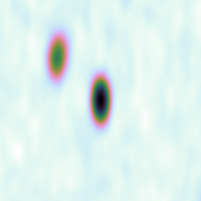
\includegraphics[width=\textwidth]{atlas-images/cdfs_100_compact.png}
            \caption{\DIFaddbeginFL \raggedright{} \DIFaddendFL Two compact components, each a compact source.}
        \end{subfigure}
        \begin{subfigure}{0.3\textwidth}
            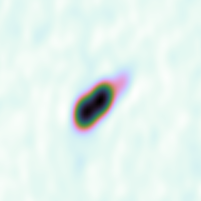
\includegraphics[width=\textwidth]{atlas-images/elais_57_resolved.png}
            \caption{\DIFaddbeginFL \raggedright{} \DIFaddendFL One resolved component and resolved source.\DIFdelbeginFL %DIFDELCMD < \\\phantom{a}%%%
\DIFdelendFL }
        \end{subfigure}
        \begin{subfigure}{0.3\textwidth}
            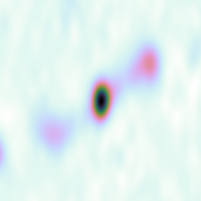
\includegraphics[width=\textwidth]{atlas-images/cdfs_185_resolved.png}
            \caption{\DIFaddbeginFL \raggedright{} \DIFaddendFL Three resolved components comprising one resolved source.}
        \end{subfigure}
        \caption[Examples showing key definitions of radio emission regions used throughout this chapter.]{\label{fig:definitions} Examples showing key definitions of radio emission regions used throughout this chapter.
                 Compact and resolved components are defined by \autoref{eq:atlas-compact}.}
    \end{figure}

    Next generation radio telescopes such as the Australian SKA Pathfinder \citep[ASKAP;][]{johnston07} and Apertif \citep{verheijen08} will conduct increasingly wide, deep, and high-resolution radio surveys, producing large amounts of data. The Evolutionary Map of the Universe \citep[EMU;][]{norris11} survey using ASKAP is expected to detect over 70 million radio sources, compared to the 2.5 million radio sources currently known \citep{banfield15}. An important part of processing these data is cross-identifying observed radio emission regions with observations of their host \DIFdelbegin \DIFdel{galaxy }\DIFdelend \DIFaddbegin \DIFadd{galaxies }\DIFaddend in surveys at other wavelengths.

    In the presence of extended radio emission\DIFaddbegin \DIFadd{, }\DIFaddend cross-identification of the host can be a
    difficult task. {Radio emission may extend far from the host galaxy
    and emission regions from a single physical object may appear disconnected. As a result, the
    observed structure of a radio source may have a complex relationship
    with the corresponding host galaxy, and cross-identification in radio is
    much more difficult than cross-identification at shorter wavelengths.} Small surveys
    containing a few thousand sources such as the Australia Telescope Large Area Survey
    \citep[ATLAS;][]{norris06, middelberg08} can be cross-identified manually,
    but this is impractical for larger surveys.

    One approach to cross-identification of large numbers of sources is crowdsourcing, where volunteers
    cross-identify radio sources with their host \DIFdelbegin \DIFdel{galaxy}\DIFdelend \DIFaddbegin \DIFadd{galaxies}\DIFaddend . This is the premise of Radio Galaxy
    Zoo\footnote{\url{https://radio.galaxyzoo.org}} \citep{banfield15}, a
    citizen science project hosted on the Zooniverse platform \citep{lintott08}.
    Volunteers are shown radio and infrared images and are asked to
    cross-identify radio sources with the corresponding infrared host galaxies. An
    explanation of the project can be found in \citet{banfield15}. The first
    data release for Radio Galaxy Zoo will provide a large dataset of over
    75~000 radio-host cross-identifications and radio source morphologies
    (Wong et al., in prep\DIFaddbegin \DIFadd{.}\DIFaddend ). While this is a much larger number of visual
    cross-identifications than have been made by experts \citep[e.g.,
    ][]{taylor2007,Gendre2008,grant2010,norris06,middelberg08} it is still far
    short of the millions of radio sources expected to be detected in upcoming
    radio surveys \citep{norris17surveys}.

    Automated algorithms have been developed for cross-identification.
    \citet{fan15} applied Bayesian
    hypothesis testing to this problem, fitting a three-component model to extended radio
    sources. This was achieved under the assumption that extended radio sources
    are composed of a core radio component and two lobe components. The core
    radio component is coincident with the host galaxy, so cross-identification
    amounts to finding the galaxy coincident with the core radio component in
    the most likely model fit. This method \DIFdelbegin \DIFdel{is }\DIFdelend \DIFaddbegin \DIFadd{could be }\DIFaddend easily extended to use other, more
    complex models, but it is purely geometric. It does not incorporate
    other information such as the physical properties of the potential host
    galaxy. Additionally, there may be new classes of radio source detected in
    future surveys like EMU which do not fit the model. \citet{weston18lrpy}
    developed a modification of the likelihood ratio method of
    cross-identification \citep{richter75likelihood} for application to ATLAS
    and EMU. This method does well on non-extended radio sources
    with approximately 70 per cent accuracy in the ATLAS fields, but does
    not currently handle more complex (extended or multi-component) radio sources
    \citep{norris17unexpected}.

    {One possibility is that machine learning techniques can
    be developed to automatically cross-identify catalogues drawn from new surveys}. Machine learning
    describes a class of methods that learn approximations to functions. {If
    cross-identification can be cast as a function approximation problem, then machine learning will allow \DIFdelbegin \DIFdel{data
    sets }\DIFdelend \DIFaddbegin \DIFadd{datasets
    }\DIFaddend such as Radio Galaxy Zoo to be generalised to work on new data. \DIFdelbegin \DIFdel{Data sets }\DIFdelend \DIFaddbegin \DIFadd{Datasets }\DIFaddend from
    citizen scientists have already been used to train machine learning methods.
    Some astronomical examples can be found in \citet{marshall15citizen}.}

    In this chapter we {cast cross-identification as a function
    approximation problem by} applying an approach from computer vision
    literature. This approach casts cross-identification as the standard machine
    learning problem of binary classification {by asking whether a given
    infrared source is the host galaxy or not}. We train our methods on expert
    cross-identifications and volunteer cross-identifications from Radio Galaxy Zoo. In
    \autoref{sec:atlas-xid-data} we describe the data we use to train our methods. In
    \autoref{sec:atlas-xid-method} we discuss how we cast the radio host galaxy
    cross-identification problem as a machine learning problem. In
    \autoref{sec:atlas-xid-results} we present results of applying our method to ATLAS
    observations of the \emph{Chandra} Deep Field South (CDFS) and the ESO Large Area ISO Survey South 1 (ELAIS-S1) field. Our data, code and results are
    available at \url{https://radiogalaxyzoo.github.io/atlas-xid}.

    {Throughout this chapter, a `radio source' refers to all radio emission observed associated with a single host galaxy, and a `radio component' refers to a single, contiguous
    region of radio emission. Multiple components may arise from a single
    source. A `compact' source is composed of a {single unresolved component. \autoref{eq:atlas-compact} shows the definition of a resolved component. We
    assume that all unresolved components are compact sources, i.e. we assume that each unresolved component has its own host galaxy\footnote{{This will be incorrect if the unresolved components are actually compact lobes or \DIFdelbegin \DIFdel{hotspots}\DIFdelend \DIFaddbegin \DIFadd{hot-spots}\DIFaddend , but determining which components correspond to unique radio sources is outside the scope of this thesis.}}.} An `extended'
    source is a non-compact source, i.e. resolved single-component sources or a
    multi-component source. \autoref{fig:definitions} illustrates these definitions.}

\section{Data}\label{sec:atlas-xid-data}

  We use radio data from the Australia Telescope Large Area Survey
  \citep[ATLAS;][]{norris06,franzen15}, infrared data from the \emph{Spitzer}
  Wide-area Infrared Extragalactic survey \citep[SWIRE;][]{lonsdale03swire,
  surace05swire}, and cross-identifications of these surveys from the citizen
  science project Radio Galaxy Zoo \citep{banfield15}. Radio Galaxy Zoo also
  includes cross-identifications of sources in Faint Images of the Radio Sky at
  Twenty Centimeters \citep[FIRST;][]{white97first} and the All\emph{WISE}
  survey \citep{cutri2013wiseexplanatory}, though we focus only on Radio
  Galaxy Zoo data from ATLAS and SWIRE.

  \subsection{ATLAS}\label{sec:atlas-xid-atlas}
    \begin{table}
      \caption[Catalogues of ATLAS/SWIRE cross-identifications for the CDFS
        and ELAIS-S1 fields.]{Catalogues of ATLAS/SWIRE cross-identifications for the CDFS
        and ELAIS-S1 fields. The method used to generate each catalogue is
        shown, along with the number of radio components cross-identified in each
        field.}
      \centering
      \label{tab:atlas-cids}
      \begin{tabular}{llcc}
        \hline\hline
        Catalogue & Method & CDFS & ELAIS-S1\\
        \hline
        \citet{norris06} & Manual & 784 & 0\\
        \citet{middelberg08} & Manual & 0 & 1366\\
        \citet{fan15} & Bayesian models & 784 & 0\\
        \citet{weston18lrpy} & Likelihood ratio & 3078 & 2113\\
        Wong et al. (in prep\DIFaddbeginFL \DIFaddFL{.}\DIFaddendFL ) & Crowdsourcing & 2460 & 0 \\
        \hline\hline
      \end{tabular}
    \end{table}

    ATLAS is a pilot survey for the EMU \citep{norris11} survey, which will
    cover the entire sky south of $+30$ deg and is expected to detect
    approximately 70 million new radio sources. {95 per cent of these sources
    will be single-component sources, but the remaining 5 per cent pose a
    considerable challenge to current automated cross-identification methods
    \citep{norris11}.} EMU will be conducted at the same depth and resolution
    as ATLAS, so methods developed for processing ATLAS data are expected to
    work for EMU. ATLAS is a wide-area radio survey of the CDFS and ELAIS-S1
    fields at 1.4~GHz with a sensitivity of 14 and
    \unit{17}{\micro\jansky}~beam$^{-1}$ on CDFS and ELAIS-S1 respectively.
    CDFS covers 3.6~deg$^2$ and contains 3034 radio components above a
    signal-to-noise ratio of 5. ELAIS-S1 covers 2.7~deg$^2$ and contains 2084
    radio components above a signal-to-noise ratio of 5 \citep{franzen15}. The
    images of CDFS and ELAIS-S1 have angular resolutions of 16 by 7 and 12 by
    8 arcsec respectively, with pixel sizes of 1.5 arcsec px$^{-1}$.
    \autoref{tab:atlas-cids} summarises catalogues that contain
    cross-identifications of radio components in ATLAS with host galaxies in
    SWIRE. In the present work, we train methods on
    CDFS\footnote{{Radio Galaxy Zoo only contains CDFS sources and so
    we cannot train methods on ELAIS-S1.}} and test these methods on both CDFS
    and ELAIS-S1. This \DIFdelbegin \DIFdel{ensures }\DIFdelend \DIFaddbegin \DIFadd{helps confirm that }\DIFaddend our methods are transferable to different
    areas of the sky observed by the same telescope\DIFaddbegin \DIFadd{, }\DIFaddend as will be the case for
    EMU.

  \subsection{SWIRE}\label{sec:atlas-xid-swire}

    SWIRE is a wide-area infrared
    survey at the four IRAC wavelengths 3.6, 4.5, 5.8, and
    \unit{8.0}{\micro\meter} \citep{lonsdale03swire, surace05swire}. It covers eight fields, including CDFS and ELAIS-S1. SWIRE is the source of infrared
    observations for cross-identification with ATLAS. SWIRE has catalogued 221,535
    infrared objects in CDFS and 186,059 infrared objects in ELAIS-S1 above a signal-to-noise ratio of 5.

  \subsection{Radio Galaxy Zoo}\label{sec:atlas-xid-rgz}

    Radio Galaxy Zoo asks volunteers to cross-identify radio components with
    their infrared host galaxies. There are a total of 2460 radio components
    in Radio Galaxy Zoo sourced from ATLAS {observations of CDFS}. These components are
    cross-identified by Radio Galaxy Zoo participants with host galaxies
    detected in SWIRE. A more detailed description can be found in
    \citet{banfield15} and a full description of how the Radio Galaxy Zoo catalogue used in this work\footnote{The Radio Galaxy Zoo Data
    Release 1 catalogue will only include cross-identifications for which over
    65 per cent of volunteers agree. However, we use a preliminary catalogue containing volunteer
    cross-identifications for all components.} is generated can be found in Wong
    et al. (in prep\DIFaddbegin \DIFadd{.}\DIFaddend ).

    The ATLAS~CDFS radio components that appear in Radio Galaxy Zoo {are drawn from a prerelease version of} the third data release
    of ATLAS by \citet{franzen15}. In this release, each radio component was fit with a
    two-dimensional Gaussian. Depending on the residual of the fit, more than
    one Gaussian may be fit to one region of radio emission. Each of these
    Gaussian fits is listed as a radio component in the ATLAS component catalogue. The
    brightest radio component from the multiple-Gaussian fit is called the
    `primary component'. {If there \DIFdelbegin \DIFdel{was }\DIFdelend \DIFaddbegin \DIFadd{is }\DIFaddend only one Gaussian fit then this Gaussian is the primary component}. Each primary component found in the ATLAS
    component catalogue appears in Radio Galaxy Zoo. Non-primary components
    may appear within the image of a primary component, but do not have their
    own entry in Radio Galaxy Zoo. We will henceforth only discuss the primary
    components.

  \section{Method}\label{sec:atlas-xid-method}
    \begin{figure}
      \centering
      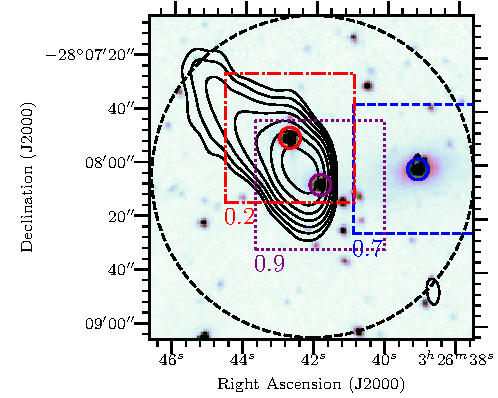
\includegraphics[width=0.6\columnwidth]{atlas-images/figure_example_of_method.pdf}
      \caption[An example of {finding} the host galaxy of a radio source using
        our sliding-window method.]{An example of {finding} the host galaxy of a radio source using
        our sliding-window method. The background image is a \unit{3.6}{\micro\meter} image from SWIRE. The contours show ATLAS radio data and start at $4\sigma$, increasing geometrically by a factor of 2. Boxes represent `windows'
        centred on {candidate host galaxies, which are circled. The pixels in each window are used to represent the candidate that the window is centred
        on. The scores of each candidate would be calculated by a binary classifier using the window as input,
        and these scores are shown below each window}. The scores
        shown are for illustration only. In this example,
        {the galaxy coincident with the centre window would be chosen as the host galaxy, as this
        window has the highest score.
        The dashed circle
        shows the $1'$ radius from which candidate host galaxies are selected. For clarity, not all candidate host galaxies are shown.}}
      \label{fig:windows}
    \end{figure}

  {The aim of this chapter is to express cross-identification in a form that
  will allow us to apply standard machine learning tools and methods. We use an approach from computer vision
  to cast cross-identification as binary classification.}

  \subsection{Cross-identification as binary classification}\label{sec:atlas-xid-as-binary-classification}
    \begin{figure}
      \centering
      %
      \tikzstyle{decision} = [diamond, draw, fill=white,
          text width=4.5em, text badly centered, inner sep=0pt]
      \tikzstyle{block} = [rectangle, draw, fill=white,
          text width=5em, text centered, rounded corners, minimum height=4em]
      \tikzstyle{line} = [draw, -latex']
      \begin{tikzpicture}[node distance=6mm, auto]
        \node [block] (init) {input radio source};
        \node [decision, right= of init] (iscompact) {compact?};
        \node [block, below= of iscompact] (compact) {find nearest infrared object};
        \node [block, right= of iscompact] (resolved) {find nearby infrared objects};
        \node [block, fill=black!30, right= of resolved] (classify) {classify objects};
        \node [block, below= of classify] (best) {choose object based on {score}};
        \coordinate (middle) at ($(compact)!0.5!(best)$);
        \node [block, below= of middle, fill=green!40] (done) {\textbf{host galaxy}};
        \path [line] (init) -- (iscompact);
        \path [line] (iscompact) -- (compact) node [midway] {yes};
        \path [line] (compact) -- (done);
        \path [line] (iscompact) -- (resolved) node [midway] {no};
        \path [line] (resolved) -- (classify);
        \path [line] (classify) -- (best);
        \path [line] (best) -- (done);
      \end{tikzpicture}
      \caption[Our cross-identification method once a binary classifier has been trained.]{{Our cross-identification method once a binary classifier has been trained}. As
        input we accept a radio {component. If the component is compact, we assume it is a compact source and select
        the nearest infrared object as the host galaxy. If the component is
        resolved, we use the binary classifier to score all nearby infrared objects
        and select the highest-scored object as the host galaxy. Compact and resolved components are defined in \autoref{eq:atlas-compact}.}}
      \label{fig:flowchart}
    \end{figure}

    We propose a two-step method for host galaxy cross-identification
    {which we will describe now}. Given a radio component, we want to find
    the corresponding host galaxy. The input is a $2' \times
    2'$ radio image of
    the sky centred on a radio component {and potentially other information about
    objects in the image (such as the redshift or infrared colour)}. {Images at other wavelengths (notably infrared) might be
    useful, but we defer this for now as it complicates the task.
    {We \DIFdelbegin \DIFdel{chose }\DIFdelend \DIFaddbegin \DIFadd{choose }\DIFaddend a $2' \times 2'$ image to match} the size of the images used
    by Radio Galaxy Zoo. To avoid solving the separate task of identifying
    which radio components are associated with the same source, we assume
    that each radio image represents a single extended
    source\footnote{Limitations of this assumption are discussed in
    \autoref{sec:atlas-xid-limitations}.}. Radio cross-identification can then
    be formalised as follows: \DIFdelbegin \DIFdel{given }\DIFdelend \DIFaddbegin \DIFadd{Given }\DIFaddend a radio image centred on a radio
    component, locate the host galaxy of the source containing this radio
    component. This is a standard computer vision problem called `object
    detection', and we apply a common technique called a `sliding-window'
    \citep{rowley1996facedetection}}.

    {In sliding-window object detection, we want to find an object in an image.
    We develop a function to score each location in the image such that the
    highest-scored location coincides with the desired object. Square image
    cutouts called `windows' are taken centred on each location and these
    windows are used to represent that location in our scoring function. To
    find the infrared host galaxy, we choose the location with the highest
    score. To improve the efficiency of this process when applied to
    cross-identification, we only consider windows coincident with infrared
    sources detected in SWIRE. We call these infrared sources `candidate
    host galaxies'. For this chapter, there is no use in scoring
    locations without infrared sources as that would not lead to a host identification
    anyway. Using candidate host galaxies instead of pixels also
    allows us to include ancillary information about the candidate host
    galaxies, such as their infrared colours and redshifts. We refer to the
    maximum distance a candidate host galaxy can be separated from a radio component as
    the `search radius' and take this radius to be $1$ arcmin. To score each
    candidate host galaxy we use a `binary classifier', which we will define
    now.}

    \begin{algorithm}
        \KwData{\\\quad{}A $2 \times 2$ arcmin radio image of a radio component%
                \\\quad{}A set of infrared candidate host galaxies $\mathcal G$%
                \\\quad{}A binary classifier $f : \mathbb R^k \to \mathbb{R}$}
        \KwResult{A galaxy $g \in \mathcal G$}

        $max \leftarrow -\infty$\;
        $host \leftarrow \emptyset$\;
        \For{$g \in \mathcal G$}{
          $x \leftarrow$ a $k$-dimensional vector representation of $g$ (\autoref{vector-representation-of-infrared-sources})\;
          $d \leftarrow$ distance between $g$ and the radio component\;
          $score \leftarrow f(x) \times \frac{1}{\sqrt{2\pi\sigma^2}} \exp\left(-\frac{d^2}{2\sigma^2}\right);$
          \BlankLine
          \If{$score > max$}{
            $max \leftarrow score$\;
            $host \leftarrow g$\;
          }
        }

        \KwRet{$host$}
        \caption{Cross-identifying a radio component given a radio image of the component, a catalogue of infrared candidate host galaxies\DIFaddbegin \DIFadd{, }\DIFaddend and a binary classifier.
          {$\sigma$ is a parameter of the method.}}
        \label{alg:xid}
    \end{algorithm}

    {Binary classification is a common method in machine learning
    where objects are to be assigned to one of two classes,
    called the `positive' and `negative' classes. This assignment is
    represented by the probability that an object is in the positive class. A
    `binary classifier' is a function mapping from an object to such a
    probability. Our formulation of cross-identification is equivalent to
    binary classification of candidate host galaxies: the positive class
    represents host galaxies, the negative class represents non-host galaxies,
    and to cross-identify a radio component we find the candidate host galaxy
    maximising the positive class probability. In other words,
    the binary classifier is exactly the sliding-window scoring function. We therefore split
    cross-identification into two separate tasks: the `candidate
    classification task' where, given a candidate host galaxy, we wish to
    determine whether it is a host galaxy of \emph{any} radio component; and
    the `cross-identification task' where, given a specific radio
    component, we wish to find its host galaxy. The candidate classification task
    is a traditional machine learning problem which results in a binary
    classifier. To avoid ambiguity and recognise that the values output by a
    binary classifier are not true probabilities, we will refer to the outputs
    of the binary classifier as `scores' in line with the sliding-window approach
    described above. The cross-identification task maximises over scores
    output by this classifier. Our approach is illustrated in
    \autoref{fig:windows} and described in \autoref{alg:xid}. We refer to the
    binary classifier scoring a candidate host galaxy as
    $f$. To implement $f$ as a function that accepts candidate host galaxies
    as input, we need to represent candidate host galaxies by vectors. We
    describe this in \autoref{vector-representation-of-infrared-sources}.
    There are many options for modelling $f$. In this chapter we apply three
    different models: logistic regression, random forests\DIFaddbegin \DIFadd{, }\DIFaddend and convolutional
    neural networks.}

    {We cross-identify each radio component in turn. The classifier $f$
    provides a score for each candidate host galaxy. This score indicates how
    much the candidate looks like a host galaxy, independent of which radio
    component we are currently cross-identifying. If there are other nearby host
    galaxies, then multiple candidate hosts may have high scores (e.g.
    \autoref{fig:broken-isolation}). This difficulty is necessary---a classifier
    with dependence on \DIFaddbegin \DIFadd{the }\DIFaddend radio object would be impossible to train. We
    need multiple positive examples (i.e. host galaxies) to train a binary classifier, but
    for any specific radio component there is only one host galaxy. As a
    result, the candidate classification task aims to answer the general question
    of whether a given galaxy is the host galaxy of \emph{any} radio
    component, while the cross-identification task attempts to cross-identify
    a \emph{specific} radio component. To distinguish between candidate host
    galaxies with high scores, we weight the scores by a Gaussian function of
    angular separation between the candidates and the radio component.} The
    width of the Gaussian, $\sigma$, controls the influence of the Gaussian on
    the final cross-identification. When $\sigma$ is small, our approach is
    equivalent to a nearest neighbours approach where we select the nearest
    infrared object to the radio component as the host galaxy. In the limit
    where $\sigma \to \infty$, we maximise the score output by the
    classifier as above. We take $\sigma = 30''$\DIFdelbegin \DIFdel{as this was }\DIFdelend \DIFaddbegin \DIFadd{, }\DIFaddend the best value
    found by a grid search \DIFaddbegin \DIFadd{maximising cross-identification accuracy}\DIFaddend . {Note that the optimum width \DIFdelbegin \DIFdel{will depend }\DIFdelend \DIFaddbegin \DIFadd{depends }\DIFaddend on
    the density of radio sources on the sky, the angular separation of the
    host galaxy and its radio components and the angular resolution of the survey.}

    {We can improve upon this method by cross-identifying compact radio sources
    separately from extended sources, as compact sources are much easier to
    cross-identify. For a compact source, the nearest SWIRE object may be
    identified as the host galaxy (a \emph{nearest neighbours} approach), or a
    more complex method such as likelihood ratios may be applied
    \citep[see][]{weston18lrpy}. We cross-identify compact sources separately
    in our pipeline and this process is shown in \autoref{fig:flowchart}.}

  \subsection{Limitations of our approach}
    \label{sec:atlas-xid-limitations}

    \begin{figure}
      \centering
      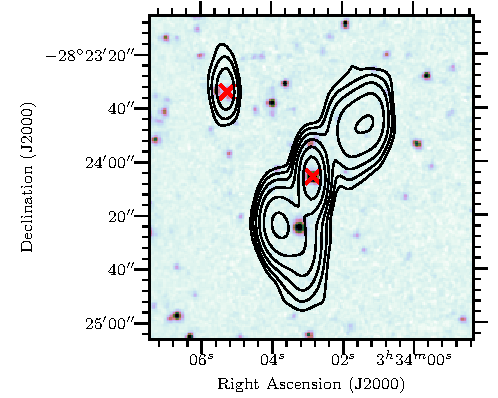
\includegraphics[width=0.6\linewidth]{atlas-images/CI0077C1_fig.pdf}
      \caption[A radio source breaking our assumption that there are no other radio sources with 1~arcmin of the source.]{A $2'$-wide radio image centred on ATLAS3\textunderscore{}J033402.87-282405.8C.
        %
        This radio source breaks the assumption that there are no other radio
        sources within 1~arcmin of the source. Another radio source is visible
        to the upper-left. Host galaxies found by Radio Galaxy Zoo volunteers
        are shown by crosses. {The background image
        is a \unit{3.6}{\micro\meter} image from SWIRE. The contours show ATLAS radio data and start at $4\sigma$, increasing geometrically by a factor of 2.}}
      \label{fig:broken-isolation}
    \end{figure}

    \begin{figure}
      \centering
      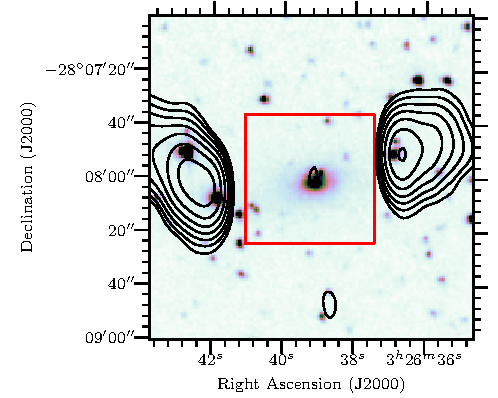
\includegraphics[width=0.6\linewidth]{atlas-images/CI2363_fig.pdf}
      \caption[A radio source where the window centred on the host galaxy does not contain enough radio information to correctly identify the galaxy as a host.]{An example of a radio source where the window centred on the
        host galaxy, shown as a rectangle, does not contain enough radio
        information to correctly identify the galaxy as the host. {The background image
        is a \unit{3.6}{\micro\meter} image from SWIRE. The contours show ATLAS radio data and start at $4\sigma$, increasing geometrically by a factor of 2.}}
      \label{fig:broken-window-size}
    \end{figure}

    \begin{figure}
      \centering
      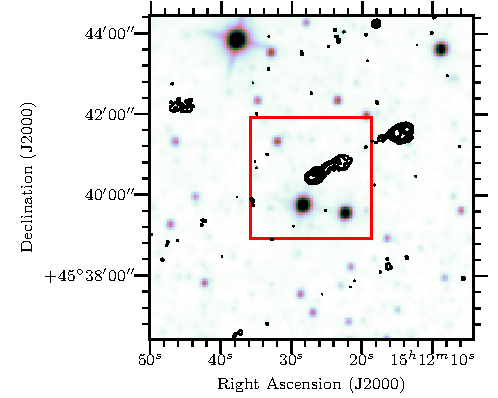
\includegraphics[width=0.6\linewidth]{atlas-images/FIRSTJ151227_fig.pdf}
      \caption[A radio source breaking our assumption that the whole radio source is visible in the chosen radius.]{A $8'$-wide radio image from FIRST, centred on
        FIRST\ J151227.2+454026. The $3'$-wide red box indicates the boundaries of
        the image of this radio component shown to volunteers in Radio Galaxy
        Zoo. This radio source breaks our assumption that the whole radio source
        is visible in the chosen radius. As one of the {components} of the radio source
        is outside of the image, a volunteer (or automated algorithm) looking at
        the $3'$-wide image may be unable to determine that this is a radio
        double or locate the host galaxy. {The background image
        is a \unit{3.4}{\micro\meter} image from \emph{WISE}. The contours show FIRST radio
        data, starting at $4\sigma$ and increasing geometrically by a factor of 2.}}
      \label{fig:broken-contains}
    \end{figure}

    We make a number of assumptions to relate the cross-identification task to
    the candidate classification task:
    \begin{enumerate}
      \item {For any radio component, the $2' \times 2'$ image centred on the component contains components of only one radio source.}
      \item {For any radio component, the $2' \times 2'$ image centred on the component contains all components of this source.}
      \item The host galaxy of a radio component is within the 1~arcmin {search radius around the component, measured from the centre of the Gaussian fit}.
      \item The host galaxy of a radio component is closer on the sky to the
        radio component than the host galaxy of any other radio component.
      \item The host galaxy appears in the SWIRE catalogue.
    \end{enumerate}
    These assumptions limit the effectiveness of our approach, regardless of
    how accurate our binary classifier may be. {Examples of radio sources that break these respective assumptions are:}
    \begin{enumerate}
      \item {A radio source less than $1'$ away from another radio source.}
      \item {A radio source with an angular size greater than $2'$.}
      \item {A radio source with a component greater than $1'$ away from the host galaxy.}
      \item {A two-component radio source with another host galaxy between a component and the true host galaxy.}
      \item {An infrared-faint radio source \citep[as in][]{collier14irfaint}.}
    \end{enumerate}

    {The main limitations are problems of scale in choosing the
    candidate search radius and the size of the windows
    representing candidates. If the search radius is too small, we may not
    consider the host galaxy as a candidate. If the search radius is too
    large, we may consider multiple host galaxies (though this is mostly
    mitigated by the Gaussian weighting). If the window is too small, radio
    emission may extend past the edges of the window and we may miss critical
    information required to identify the galaxy as a host galaxy. If the
    window is too large, then irrelevant information will be included and it
    may be difficult or computationally expensive to score. We \DIFdelbegin \DIFdel{chose }\DIFdelend \DIFaddbegin \DIFadd{choose }\DIFaddend a
    window size of $32 \times 32$ pixels, corresponding to approximately $48'' \times 48''$ in
    ATLAS. This is shown as squares in \autoref{fig:windows} and
    \autoref{fig:broken-window-size}. These kinds of size problems are
    difficult even for non-automated methods as radio sources can be extremely
    wide---for example, Radio Galaxy Zoo found a radio giant that spanned
    over three different images presented to volunteers and the full source
    was only cross-identified by the efforts of citizen scientists
    \citep{banfield15}. An example of a radio image where part of the radio
    source is outside the search radius is shown in
    \autoref{fig:broken-contains}.}

    In weighting the scores by a Gaussian function of angular
    separation, we implicitly assume that the host galaxy of a radio component
    is closer to that radio component than any other host galaxy. If this
    assumption is not true then the incorrect host galaxy may be identified, though
    this is rare.

    We only need to require that the host galaxy appears in SWIRE to
    incorporate galaxy-specific features
    (\autoref{vector-representation-of-infrared-sources}) and to improve
    efficiency. Our method is applicable even when host galaxies are not detected in
    the infrared by considering every pixel of the radio image as a candidate
    location as would be done in the original computer vision approach. {If the host galaxy location does not correspond to an infrared source, the radio source \DIFdelbegin \DIFdel{would }\DIFdelend \DIFaddbegin \DIFadd{can }\DIFaddend be classified as infrared-faint.}

    Our assumptions impose an upper bound on how well we can cross-identify
    radio sources. We estimate this upper bound in \autoref{sec:atlas-xid-cdfs-results}.

  \subsection{Feature vector representation of infrared sources}
  \label{vector-representation-of-infrared-sources}

    {Inputs to binary classifiers must be represented by an array of real values called feature vectors.} We therefore need to choose a feature vector representation of our candidate host galaxies. Candidate hosts are sourced from the SWIRE catalogue (\autoref{sec:atlas-xid-swire}). We represent each candidate host with 1034 real-valued features, {combining the windows centred on each candidate (\autoref{sec:atlas-xid-as-binary-classification}) with ancillary infrared data from the SWIRE catalogue}. For a given candidate host, these features are:
    \begin{itemize}
      \item the 6 base-10 logarithms of the ratios of fluxes of the candidate
        host at the four IRAC wavelengths {(the `colours' of the candidate)};
      \item the flux of the host at \unit{3.6}{\micro\meter};
      \item the stellarity index of the host at both 3.6 and
        \unit{4.5}{\micro\meter};
      \item the radial distance between the candidate host and the nearest
        radio component in the ATLAS catalogue; and
      \item a 32 $\times$ 32 pixel image from ATLAS (approximately $48''
        \times 48''$), centred on the candidate host {(the window)}.
    \end{itemize}

    The infrared colours provide insight into the properties {of the candidate
    host galaxy} \citep{grant11polarised}. The 3.6 and \unit{4.5}{\micro\meter} fluxes trace
    both galaxies with faint polycyclic aromatic hydrocarbon (PAH) emission {(i.e. late-type, usually star-forming galaxies)}
    and elliptical galaxies dominated by old stellar populations. The
    \unit{5.8}{\micro\meter} flux selects galaxies where the infrared emission
    is dominated by non-equilibrium emission of dust grains {due to active galactic nuclei},
    while the \unit{8.0}{\micro\meter} flux
    traces strong PAH emission at low redshift \citep{sajina2005}. The
    stellarity index {is a value in the SWIRE catalogue that represents how likely the object is to be a star rather
    than a galaxy \citep{surace05swire}. It was estimated by a neural network in
    \texttt{SExtractor} \citep{bertin96sextractor}}.

    We use the $32 \times 32$ pixels of each radio window as independent
    features for all binary classification models, with the convolutional neural
    network automatically extracting features that are relevant. Other
    features of the radio components may be used instead of just relying on the pixel values,
    but there has been limited research on extracting such features:
    \citet{proctor06} describes hand-selected features for radio doubles in
    FIRST, and \citet{aniyan17cnn} and \citet{lukic18compact} make use of
    deep convolutional neural networks which automatically extract features as
    part of classification. A more comprehensive investigation of features is
    a good avenue for potential improvement in our pipeline but this is beyond
    the scope of this initial study.

  \subsection{Binary \DIFdelbegin \DIFdel{Classifiers}\DIFdelend \DIFaddbegin \DIFadd{classifiers}\DIFaddend }\label{sec:atlas-xid-classifiers}

    We use three different binary classification models: logistic regression,
    convolutional neural networks, and random forests. These models cover
    three different approaches to machine learning. Logistic regression is a
    probabilistic binary classification model. It is linear in the feature
    space and outputs the probability that the input has a positive
    label~\citep[Chap. 4]{bishop06ml}. Convolutional neural networks (CNN) are
    biologically-inspired prediction models with image inputs.
    They have recently produced good results on large image-based datasets in
    astronomy \citep[e.g.]{lukic18compact, dieleman15cnn}. Random
    forests are an ensemble of decision trees~\citep{breiman01random-forest}.
    They consider multiple subsamples of the training set, where each
    bootstrap subsample is sampled with replacement from the training set. To
    classify a new data point, the random forest takes the weighted average of
    all classifications produced by each decision tree. \DIFaddbegin \DIFadd{For a more detailed description of these models, see }\aref{sec:atlas-xid-models}\DIFadd{.
}\DIFaddend 

  \subsection{Labels}\label{sec:atlas-xid-labels}

    \begin{figure}
      \centering
      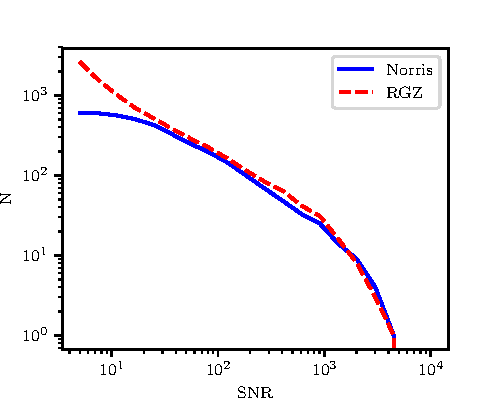
\includegraphics[width=0.6\columnwidth]{atlas-images/snr_cutoff_cumulative.pdf}
      \caption[Cumulative number of radio components in the expert and Radio Galaxy
        Zoo training sets with different signal-to-noise ratios.]{Cumulative number of radio components ($N$) in the expert (Norris) and Radio Galaxy
        Zoo (RGZ) training sets with different signal-to-noise ratios (SNR).}
      \label{fig:distribution-cutoffs}
    \end{figure}

    \begin{figure}
      \centering
      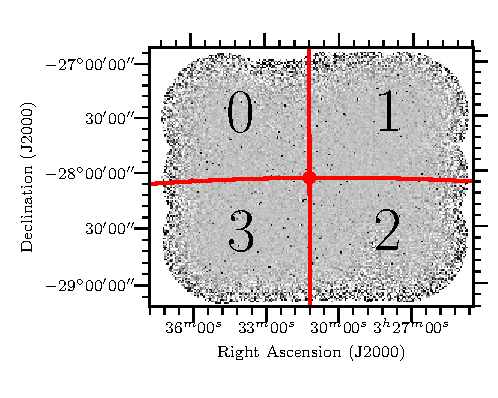
\includegraphics[width=0.6\columnwidth, trim={0cm 0.5cm 0cm 0.5cm}, clip]{atlas-images/quadrants.pdf}
      \caption[CDFS field training and testing quadrants.]{CDFS field training and testing quadrants labelled 0 -- 3. The
        central dot is located at $\alpha = 03^\text{h}31^\text{m}12^\text{s},
        \delta = -28^\circ{}06'00''$. The quadrants \DIFdelbeginFL \DIFdelFL{were }\DIFdelendFL \DIFaddbeginFL \DIFaddFL{are }\DIFaddendFL chosen such that
        there are similar numbers of radio sources in each
        quadrant.\label{fig:quadrants}}
    \end{figure}

    \begin{table}
      \caption[Number of compact and resolved radio objects in each CDFS
      quadrant.]{Number of compact and resolved radio objects in each CDFS
      quadrant. Radio Galaxy Zoo (RGZ) has more cross-identifications than the
      expert catalogue \citep{norris06} provides as it uses a deeper data release of ATLAS, and
      so has more objects in each quadrant for training.}
      \label{tab:radio-count}
      \centering
      \begin{tabular}{lcccc}
        \hline\hline
        Quadrant & Compact & Resolved & Compact & Resolved\\
        &&&(RGZ)&(RGZ)\\
        \hline
        0 & 126 & 24 & 410 & 43 \\
        1 & 99 & 21 & 659 & 54 \\
        2 & 61 & 24 & 555 & 57 \\
        3 & 95 & 18 & 631 & 51 \\
        \hline
        \textit{Total} & 381 & 87 & 2255 & 205\\
        \hline\hline
      \end{tabular}
    \end{table}

    {The Radio Galaxy Zoo and \citet{norris06} cross-identification
    catalogues must be converted to binary labels for infrared objects so that
    they can be used to train binary classifiers. There are two challenges with this conversion:
    \begin{itemize}
      \item We can only say that an object is \emph{a} host galaxy, not which radio object it is associated with, and
      \item We cannot disambiguate between non-host infrared objects and host galaxies that \DIFdelbegin \DIFdel{were }\DIFdelend \DIFaddbegin \DIFadd{are }\DIFaddend not in the cross-identification catalogue.
    \end{itemize}

    We use the Gaussian weighting described in \autoref{sec:atlas-xid-as-binary-classification} to address the first issue.
    The second issue is known as a `positive-unlabelled' classification problem, which is
    a binary classification problem where we only observe labels for the
    positive class. We treat unlabelled objects as negative examples following
    \citet{menon15cpe}. That is, we make the na\"ive assumption that any
    infrared object in the SWIRE catalogue not identified as a host galaxy in a cross-identification catalogue is not a host galaxy at all.}

    We first generate positive labels from a cross-identification catalogue.
    We decide that if an infrared object is listed in the catalogue, then it
    is assigned a positive label as a host galaxy. We then assign every other galaxy a negative label. This has some \DIFdelbegin \DIFdel{problems
   ---an }\DIFdelend \DIFaddbegin \DIFadd{problems---an }\DIFaddend example is that if the cross-identification catalogue \DIFdelbegin \DIFdel{did }\DIFdelend \DIFaddbegin \DIFadd{does }\DIFaddend not include a radio
    object (e.g.~it \DIFdelbegin \DIFdel{was }\DIFdelend \DIFaddbegin \DIFadd{is }\DIFaddend below the signal-to-noise ratio) then the host galaxy
    of that radio object \DIFdelbegin \DIFdel{would receive }\DIFdelend \DIFaddbegin \DIFadd{receives }\DIFaddend a negative label. This occurs with
    \citet{norris06} cross-identifications, as these are associated with the
    first data release of ATLAS. The first data release went to a 5$\sigma$
    flux density level of $S_{1.4} \geq \unit{200}{\micro\jansky}\text{
    beam}^{-1}$ \citep{norris06}, compared to $S_{1.4} \geq \unit{85}{\micro\jansky}\text{
    beam}^{-1}$ for the third data release used by Radio Galaxy Zoo
    \citep{franzen15}. The labels from \citet{norris06} may therefore disagree with labels
    from Radio Galaxy Zoo even if they are both plausible. The difference in
    training set size at different flux cutoffs is shown in
    \autoref{fig:distribution-cutoffs}. We train and test our binary
    classifiers on infrared objects within a 1~arcmin radius of an ATLAS radio
    component.

  \subsection{Experimental \DIFdelbegin \DIFdel{Setup}\DIFdelend \DIFaddbegin \DIFadd{setup}\DIFaddend }
  \label{sec:atlas-xid-experimental-setup}

    We trained binary classifiers on infrared objects in the CDFS field using
    two sets of labels. One label set was derived from Radio Galaxy Zoo
    cross-identifications and the other was derived from the \citet{norris06}
    cross-identification catalogue. We refer to these as the `Radio Galaxy Zoo
    labels' and the `expert labels' respectively. We divided the CDFS field
    into four quadrants for training and testing. The quadrants were divided
    with a common corner at $\alpha = 03^\text{h}31^\text{m}12^\text{s},
    \delta = -28^\circ{}06'00''$ as shown in \autoref{fig:quadrants}. For
    each trial, one quadrant was used to extract test examples and the other
    three quadrants were used for training examples.

    We further divided the radio components into compact and resolved. Compact
    components are cross-identified by fitting a 2D Gaussian \citep[as
    in][]{norris06} and we would expect any machine learning approach for host
    cross-identification to attain high accuracy on this set. A radio component was
    considered resolved if
    \begin{equation}
      \label{eq:atlas-compact}
        \ln \left(
          \frac{S_{\text{int}}}{S_{\text{peak}}}
        \right) > 2\sqrt{\left(
          \frac{\sigma_{S_{\text{int}}}}{S_{\text{int}}}
        \right)^2 + \left(
          \frac{\sigma_{S_{\text{peak}}}}{S_{\text{peak}}}
        \right)^2}\,\,\,\,,
    \end{equation}%
    where \(S_{\text{int}}\) is the integrated flux density,
    \(S_{\text{peak}}\) is the peak flux density, {$\sigma_{S_{\text{int}}}$ is
    the uncertainty in integrated flux density and $\sigma_{S_{\text{peak}}}$
    is the uncertainty in peak flux density} \citep[following][]{franzen15}.

    Candidate hosts were selected from the SWIRE catalogue. For a given subset
    of radio components, all SWIRE objects within 1~arcmin of all radio
    components in the subset were added to the associated SWIRE subset. In results
    for the candidate classification task, we refer to SWIRE objects
    within 1~arcmin of a compact radio component as part of the `compact set',
    and SWIRE objects within 1~arcmin of a resolved radio component as part of
    the `resolved set'.

    To reduce bias in the testing data due to the expert labels being
    generated from a shallower data release of ATLAS, a SWIRE object was only
    included in the test set if it was within 1~arcmin of a radio object with
    a SWIRE cross-identification in both the \citet{norris06} catalogue and the
    Radio Galaxy Zoo catalogue.

    Each binary classifier was trained on the training examples and used to
    {score the test examples. These scores were thresholded to generate labels which could be directly compared
    to the expert labels. We then computed the `balanced accuracy' of these predicted labels.} Balanced
    accuracy is the average of the accuracy on the positive class and the
    accuracy on the negative class, and is not sensitive to class imbalance.
    The candidate classification task has highly imbalanced classes---in our
    total set of SWIRE objects within 1~arcmin of an ATLAS object, only 4 per
    cent have positive labels. {Our threshold was chosen to maximise the balanced
    accuracy on predicted labels of the training set.} Only examples within 1~arcmin of ATLAS objects
    in the first ATLAS data release \citep{norris06} were used to compute
    balanced accuracy, as these were the only ATLAS objects with expert labels.

    We then used the scores to predict the host galaxy
    for each radio component cross-identified by both \citet{norris06} and
    Radio Galaxy Zoo. {We followed \autoref{alg:xid}:
    \DIFdelbegin \DIFdel{the }\DIFdelend \DIFaddbegin \DIFadd{The }\DIFaddend score of each SWIRE object within 1~arcmin of a given radio
    component was weighted by a Gaussian function of angular separation from the
    radio component and the object with the highest
    weighted score was chosen as the host galaxy.} The
    {cross-identification accuracy} was then estimated as the
    fraction of the predicted host galaxies that matched the \citet{norris06}
    cross-identifications.

\section{Results}\label{sec:atlas-xid-results}

  In this section we present accuracies of our method trained on CDFS and
  applied to CDFS and ELAIS-S1, as well as results motivating our accuracy
  measures and estimates of upper and lower bounds for cross-identification
  accuracy using our method.

  \subsection{Application to ATLAS-CDFS}
  \label{sec:atlas-xid-cdfs-results}

    \begin{figure}
      \centering
      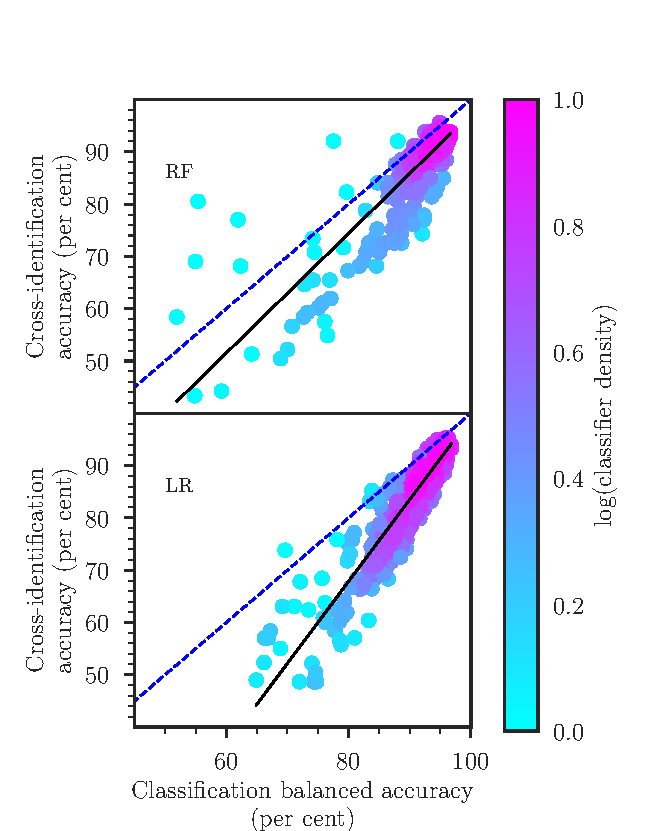
\includegraphics[width=0.6\columnwidth]{atlas-images/gct-to-xid.pdf}
      \caption[Balanced accuracy on the candidate classification task plotted
      against accuracy on the cross-identification task.]{Balanced accuracy on the candidate classification task plotted
      against accuracy on the cross-identification task. `RF' indicates
      results from random forests, and `LR' indicates results from logistic
      regression. Binary classifiers were trained on random, small subsets of the
      training data to artificially restrict their accuracies. Colour shows
      the density of points on the plot estimated by a Gaussian kernel density
      estimate. The solid lines indicate the best linear fit; these fits have
      $R^2 = 0.92$ for logistic regression and $R^2 = 0.87$ for random
      forests.
      {The dashed line shows the line where cross-identification accuracy and candidate classification accuracy are equal.}
      We did not include convolutional neural networks in this test,
      as training them is very computationally expensive. There are 640 trials shown per classification model. These results
      exclude binary classifiers with balanced accuracies less than 51 per cent, as
      these are essentially random.
      \label{fig:gct-to-xid}}
    \end{figure}

    \begin{figure}
      \centering
      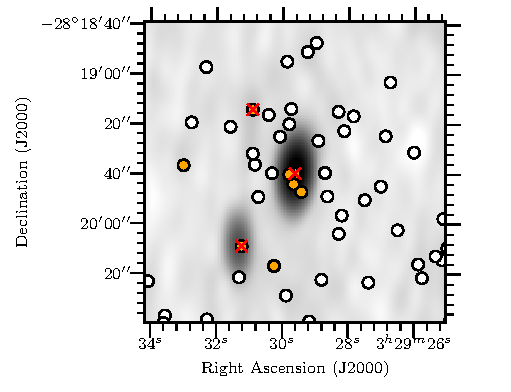
\includegraphics[width=0.6\columnwidth]{atlas-images/positives.pdf}
      \caption[An example of predicted host galaxies in the candidate classification task.]{Predicted host galaxies in the candidate classification task for ATLAS3~J032929.61-281938.9. {The background image is an ATLAS radio image.} Radio Galaxy Zoo host galaxies
      are marked by crosses. SWIRE candidate host galaxies are circles coloured by {the score output by a logistic regression binary classifier. The scores are thresholded to obtain labels, as when we compute balanced accuracy.} Orange circles have been assigned a `positive' label by a logistic regression binary classifier and white otherwise. {Note that there are more predicted host galaxies than there are radio components, so not all of the predicted host galaxies would be assigned as host galaxies in the cross-identification task.}
      \label{fig:positives}}
    \end{figure}

    \begin{figure*}
    \centering
    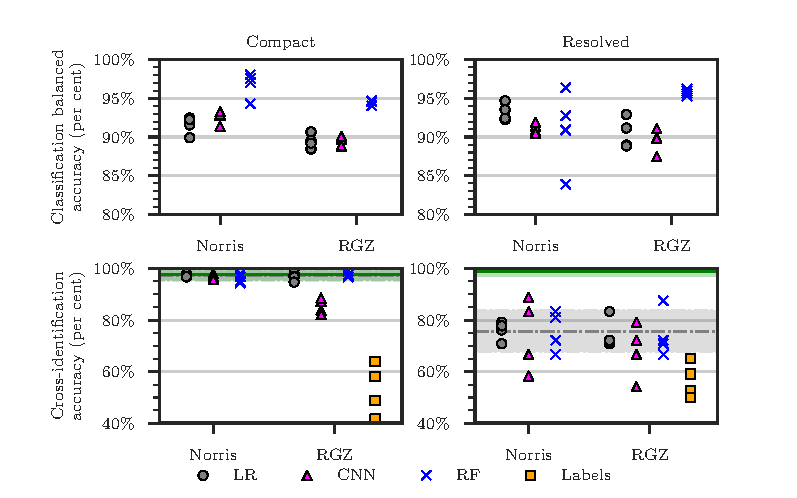
\includegraphics[width=1.0\linewidth]{atlas-images/cdfs-grid-new.pdf}
    \caption[Performance of our method with different binary classifiers on the binary classification task.]{Performance of our method with logistic regression (`LR'), convolutional neural networks (`CNN') and random forest (`RF') binary classifiers. `Norris' indicates the performance of binary classifiers trained on the expert labels and `RGZ' indicates the performance of binary classifiers trained on the Radio Galaxy Zoo labels. One point is shown per binary classifier per testing quadrant. The training and testing sets have been split into compact (left) and resolved (right) objects. {Shown for comparison is the accuracy of the Radio Galaxy Zoo consensus cross-identifications on the cross-identification task, shown as `Labels'.} The cross-identification accuracy attained by a perfect binary classifier is shown by a solid green line, and the cross-identification accuracy of a nearest neighbours approach is shown by a dashed grey line. The standard deviation of these accuracies across the four CDFS quadrants is shown by the shaded area. Note that the pipeline shown in \autoref{fig:flowchart} is not used for these results. \label{fig:ba}}
    \end{figure*}

    \begin{figure}
      \centering
      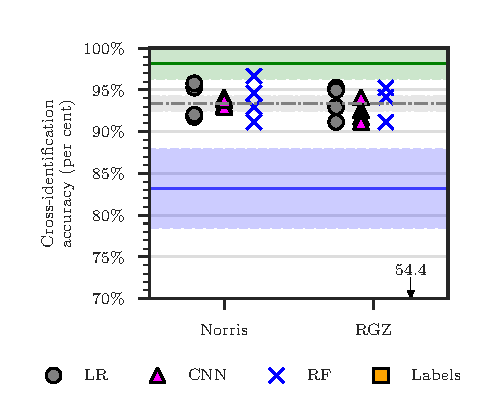
\includegraphics[]{atlas-images/cdfs_cross_identification_grid.pdf}
      \caption[Performance of our approach using different binary classifiers on the cross-identification task.]{Performance of our approach using different binary classifiers on the cross-identification task. Markers and lines are as in \autoref{fig:ba}. The blue solid line indicates the performance of a random binary classifier and represents the minimum accuracy we expect to obtain. The standard deviation of this accuracy across 25 trials and 4 quadrants is shaded. The accuracy of Radio Galaxy Zoo on the cross-identification task is below the axis and is instead marked by an arrow with the mean accuracy. Note that the pipeline shown in \autoref{fig:flowchart} is used here, {so compact objects are cross-identified in the same way regardless of binary classifier model}. \label{fig:cross-id-accuracy}}
    \end{figure}

    {We can assess trained binary classifiers either by their performance on
    the candidate classification task or by their performance on the
    cross-identification task when used in our method. Both performances are
    useful: \DIFdelbegin \DIFdel{performance }\DIFdelend \DIFaddbegin \DIFadd{Performance }\DIFaddend on the candidate classification task provides a robust
    and simple way to compare binary classifiers without the limitations of
    our specific formulation, and performance on the cross-identification task
    can be compared with other cross-identification methods. We therefore
    report two sets of accuracies: balanced accuracy for the galaxy
    classification task and accuracy for the cross-identification task. These
    accuracy measures are correlated and we show this correlation in
    \autoref{fig:gct-to-xid}. Fitting a line of best fit with \texttt{scipy}
    gives $R^2 = 0.92$ for logistic regression and $R^2 = 0.87$ for random
    forests. While performance on the candidate classification task is correlated
    with performance on the cross-identification task, balanced accuracy does
    not completely capture the effectiveness of a binary classifier applied to
    the cross-identification task. {This is because while our binary
    classifiers output real-valued scores, these scores are thresholded to
    compute the balanced accuracy}. In the candidate classification
    task, the binary classifier only needs to ensure that host galaxies are
    {scored higher} than non-host galaxies. This means
    {that after thresholding} there can be
    many `false positives' that do not affect cross-identification. An example
    of this is shown in \autoref{fig:positives}, where the classifier has
    identified \DIFdelbegin \DIFdel{8 }\DIFdelend \DIFaddbegin \DIFadd{eight }\DIFaddend `host galaxies'. However, there are only three true host
    galaxies in this image---one per radio component---and so in the
    cross-identification task, only three of these galaxies will be identified
    as hosts.}

    In \autoref{fig:ba} we plot {the balanced accuracies of our classification models
    on the candidate classification task and the cross-identification
    accuracies of our method using each of these models. Results are shown for both
    the resolved and compact sets.} For comparison, we also plot the cross-identification accuracy of Radio Galaxy
    Zoo and a nearest neighbours approach, as well as estimates for upper and
    lower limits on the cross-identification accuracy. {We estimate the upper limit on performance by assigning all
    true host galaxies a score of 1 and
    assigning all other candidate host galaxies a score of 0. This
    is equivalent to `perfectly' solving the candidate classification task and so
    represents the best possible cross-identification performance achievable
    with our method. We estimate the lower limit on performance by {
    assigning random scores to each candidate host galaxy}. We expect any
    useful binary classifier to produce better
    results than this, so this represents the lowest expected
    cross-identification performance.} The upper estimates, lower estimates,
    and \DIFdelbegin \DIFdel{nearest-neighbour }\DIFdelend \DIFaddbegin \DIFadd{nearest neighbour }\DIFaddend accuracy are shown as horizontal lines in
    \autoref{fig:ba}.

    In \autoref{fig:cross-id-accuracy} we plot the performance {of our
    method using different binary classification models}, as well as the
    performance of Radio Galaxy Zoo, nearest neighbours, and the perfect and
    random binary classifiers \DIFdelbegin \DIFdel{, }\DIFdelend on the full set of ATLAS~DR1 radio components
    using the pipeline in \autoref{fig:flowchart}. The accuracy
    {associated with each classification model} and training label set
    averaged across all four quadrants is shown in \aref{sec:atlas-xid-accuracies}.

    Differences between accuracies across training labels are well within one
    standard deviation computed across the four quadrants, with convolutional
    neural networks on compact objects as the only exception. The spread of
    accuracies is similar for both sets of training labels, with the exception
    of random forests. The balanced accuracies of random forests trained on
    expert labels have a considerably higher spread than those trained on
    Radio Galaxy Zoo labels, likely because of the small size of the expert
    training set---there are less than half the number of objects in the
    expert-labelled training set than the number of objects in the Radio
    Galaxy Zoo-labelled training set (\autoref{tab:radio-count}).

    Radio Galaxy Zoo-trained methods significantly outperform Radio Galaxy Zoo
    cross-identifications. Additionally, despite poor performance of Radio
    Galaxy Zoo on the cross-identification task, methods trained on these
    cross-identifications still perform comparably to those trained on expert
    labels. This is because incorrect Radio Galaxy Zoo cross-identifications
    can be thought of as a source of noise in the labels which is `averaged out'
    in training. This shows the usefulness of crowdsourced training data, even
    when the data is noisy.

    Our method performs comparably to a nearest neighbours approach. For
    compact objects, this is to be expected---indeed, nearest neighbours
    attains nearly 100 per cent accuracy on the compact test set. Our results
    do not improve on nearest neighbours for resolved objects. However, our
    method does allow for improvement on nearest neighbours with a
    sufficiently good binary classifier: \DIFdelbegin \DIFdel{a }\DIFdelend \DIFaddbegin \DIFadd{A }\DIFaddend `perfect' binary classifier attains
    nearly 100 per cent accuracy on resolved sources. This shows that our
    method may be useful provided that a good binary classifier can be
    trained. The most obvious place for improvement is in feature selection:
    \DIFdelbegin \DIFdel{we }\DIFdelend \DIFaddbegin \DIFadd{We }\DIFaddend use pixels of radio images directly and these are likely not conducive
    to good performance on the candidate classification task. Convolutional
    neural networks, which are able to extract features from images,
    \emph{should} work better, but these require far more training data than
    the other methods \DIFdelbegin \DIFdel{we have }\DIFdelend \DIFaddbegin \DIFadd{that we }\DIFaddend applied and the small size of ATLAS thus limits their performance.

    We noted in \autoref{sec:atlas-xid-labels} that the test set of expert labels,
    derived from the initial ATLAS data release, was less deep than the third
    data release used by Radio Galaxy Zoo and this chapter, introducing a source
    of label noise in the testing labels. Specifically, true host galaxies may
    be misidentified as non-host galaxies if the associated radio source \DIFdelbegin \DIFdel{was
    }\DIFdelend \DIFaddbegin \DIFadd{is
    }\DIFaddend below the 5 signal-to-noise limit in ATLAS~DR1 but not in ATLAS~DR3. This
    has the effect of reducing the accuracy for Radio Galaxy Zoo-trained
    classifiers.

    {We report the scores predicted by each classifier for each
    SWIRE object in \aref{sec:atlas-xid-scores} and the predicted
    cross-identification for each ATLAS object in \aref{sec:atlas-xid-xids}.
    Scores \DIFdelbegin \DIFdel{reported }\DIFdelend \DIFaddbegin \DIFadd{we report }\DIFaddend for a given object were predicted by binary
    classifiers tested on the quadrant containing that object. The reported scores are not weighted.}

    In \autoref{fig:examples} we show \DIFdelbegin \DIFdel{5 }\DIFdelend \DIFaddbegin \DIFadd{five }\DIFaddend resolved sources where the most classifiers disagreed on the correct cross-identification.

\subsection{Application to ATLAS-ELAIS-S1}
  \label{sec:atlas-xid-elais}

  \begin{figure*}
  \centering
  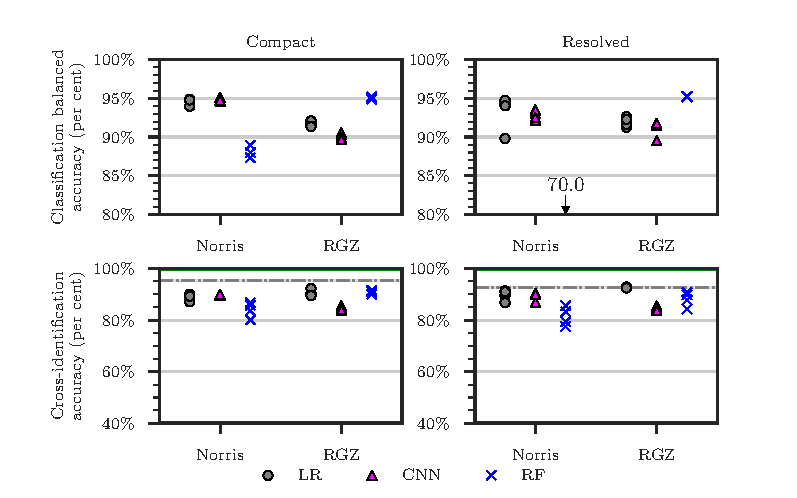
\includegraphics[]{atlas-images/elais-grid-new.pdf}
  \caption[Performance of different classification models on the binary classification task, tested on ELAIS-S1.]{Performance of different classification models trained on CDFS and tested on
  resolved and compact sources in ELAIS-S1. Points represent classification models
  trained on different quadrants of CDFS, with markers, lines\DIFaddbeginFL \DIFaddFL{, }\DIFaddendFL and axes as in
  \autoref{fig:ba}. The balanced acccuracy of expert-trained random forest
  binary classifiers falls below the axis and the corresponding mean accuracy is
  shown by an arrow. The estimated best attainable accuracy is almost 100 per cent.
    \label{fig:elais-ba}}
  \end{figure*}

  \begin{figure}
    \centering
    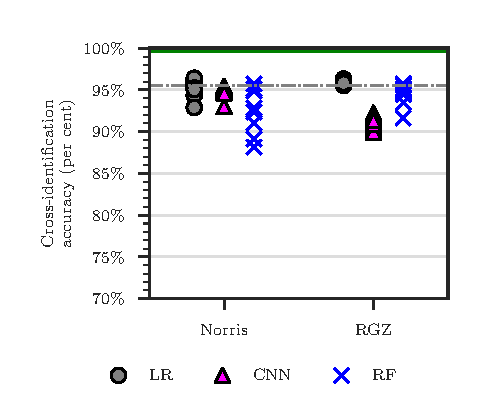
\includegraphics[]{atlas-images/elais_cross_identification_grid.pdf}
    \caption[Performance of different classification models on the cross-identification task, tested on ELAIS-S1.]{Performance of different classifiers trained on CDFS and tested
    on ELAIS-S1. Markers are as in \autoref{fig:cross-id-accuracy} and
    horizontal lines are as in \autoref{fig:elais-ba}. Note that the pipeline
    shown in \autoref{fig:flowchart} is used here, {so compact objects
    are cross-identified in the same way regardless of binary classifier
    model}.
      \label{fig:elais-cross-id-accuracy}}
  \end{figure}

  \begin{figure}
    \centering
    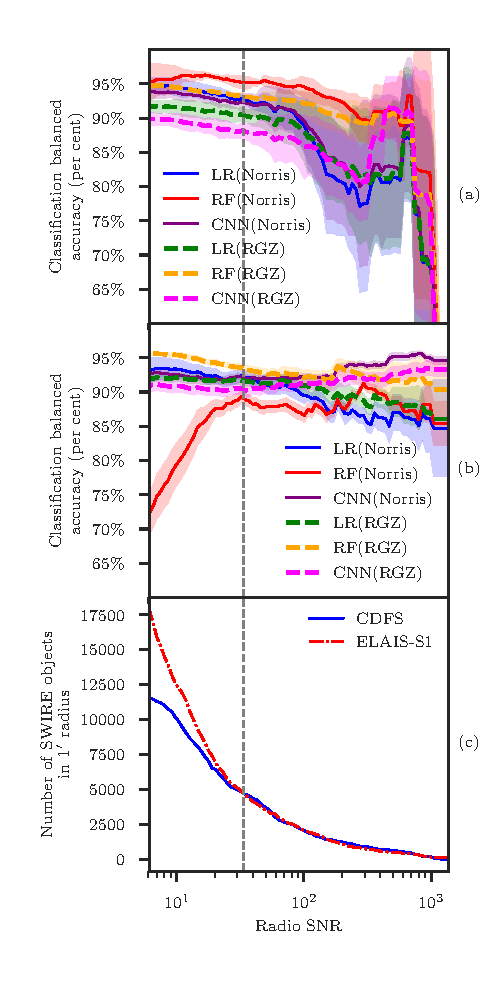
\includegraphics[trim={0cm 1cm 0cm 0.5cm}, clip]{atlas-images/accuracies-flux-snr.pdf}
    \caption[Balanced accuracies of classifiers with different SNR cutoffs.]{(a) Balanced accuracies of classifiers trained and tested on CDFS
      with different signal-to-noise ratio (SNR) cutoffs for the test set. A
      SWIRE object is included in the test set if it is within $1'$ of a radio
      component with greater SNR than the cutoff. Lines of different colour
      indicate different classifier/training labels combinations, where LR is
      logistic regression, RF is random forests, CNN is convolutional neural
      networks, and Norris and RGZ are the expert and Radio Galaxy Zoo label
      sets respectively. Filled areas represent standard deviations across
      CDFS quadrants. (b) Balanced accuracies of classifiers trained on CDFS
      and tested on ELAIS-S1. (c) A cumulative distribution plot of SWIRE
      objects associated with a radio object with greater SNR than the cutoff.
      The grey dashed line shows the SNR level at which the number of SWIRE
      objects above the cutoff is equal for CDFS and ELAIS-S1. This cutoff level
      is approximately at a SNR of $34$.}
    \label{fig:accuracies-flux}
  \end{figure}

  We applied the method trained on CDFS to perform cross-identification on the
  ELAIS-S1 field. Both CDFS and ELAIS-S1 were imaged by the same radio
  telescope to similar sensitivities and angular resolution for the ATLAS
  survey. {We can use the SWIRE cross-identifications made by
  \citet{middelberg08} to derive another set of expert labels, and hence
  determine how accurate our method is. If our method generalises well across
  different parts of the sky, then we expect CDFS-trained classifiers to have
  comparable performance between ELAIS-S1 and CDFS}. In \autoref{fig:elais-ba}
  we plot the performance of CDFS-trained classification models on the candidate classification task and
  the performance of our method on the cross-identification task using these models. We also plot
  the cross-identification accuracy of a nearest neighbours approach\footnote{{We cannot
  directly compare our method applied to ELAIS-S1 with Radio Galaxy Zoo, as
  Radio Galaxy Zoo does not include ELAIS-S1.}}. In
  \autoref{fig:elais-cross-id-accuracy} we plot the performance of our method
  on the full set of ELAIS-S1 ATLAS~DR1 radio components using the pipeline in
  \autoref{fig:flowchart}. We list the corresponding accuracies in
  \aref{sec:atlas-xid-accuracies}.

  Cross-identification results from ELAIS-S1 are similar to those for CDFS,
  showing that our method trained on CDFS performs comparably well on
  ELAIS-S1. However, nearest neighbours outperforms most methods on ELAIS-S1.
  This is likely because there is a much higher percentage of compact objects
  in ELAIS-S1 than in CDFS. The maximum achievable accuracy we have estimated
  for ELAIS-S1 is very close to 100 per cent, so (as for CDFS) a very accurate
  binary classifier would outperform nearest neighbours.

  One interesting difference between the ATLAS fields is that random forests
  trained on expert labels perform well on CDFS but poorly on ELAIS-S1. This
  is not the case for logistic regression or convolutional neural networks
  trained on expert labels, nor is it the case for random forests trained on
  Radio Galaxy Zoo. We hypothesise that this is because the ELAIS-S1
  cross-identification catalogue \citep{middelberg08} labelled fainter radio
  components than the CDFS cross-identification catalogue \citep{norris06} due
  to noise from the very bright source
  ATCDFS\textunderscore{}J032836.53-284156.0 in CDFS. Classifiers trained on
  CDFS expert labels may thus be biased toward brighter radio components
  compared to ELAIS-S1. Radio Galaxy Zoo uses a preliminary version of the third data release of ATLAS
  \citep{franzen15} and so classifiers trained on the Radio Galaxy Zoo labels
  may be less biased toward brighter sources compared to those trained on the
  expert labels. To test this hypothesis we tested each classification model against
  test sets with a signal-to-noise ratio (SNR) cutoff. A SWIRE object was only
  included in the test set for a given cutoff if it was located within $1'$ of
  a radio component with a SNR above the cutoff. The balanced accuracies for
  each classifier at each cutoff are shown in \autoref{fig:accuracies-flux}(a)
  and (b) and the distribution of test set size for each cutoff is shown in
  \autoref{fig:accuracies-flux}(c). \autoref{fig:accuracies-flux}(c) shows
  that ELAIS-S1 indeed has more faint objects in its test set than the CDFS test set, with the SNR for
  which the two fields reach the same test set size (approximately $34$)
  indicated by the dashed vertical line on each plot. For CDFS, all
  classifiers perform reasonably well across cutoffs, with performance
  dropping as the size of the test set becomes small. For ELAIS-S1, logistic
  regression and convolutional neural networks perform comparably across all
  SNR cutoffs, but random forests do not. While random forests trained on
  Radio Galaxy Zoo labels perform comparably to other classifiers across all
  SNR cutoffs, random forests trained on expert labels show a considerable
  drop in performance below the dashed line.

\section{Discussion}

  {Based on the ATLAS sample}, our main result is that it is possible
  to cast radio host galaxy cross-identification as a machine learning task
  for which standard methods can be applied. These methods can then be trained
  with a variety of label sets derived from cross-identification catalogues.
  While our methods have not outperformed nearest neighbours, we have demonstrated that
  for a very accurate binary classifier, good cross-identification results can
  be obtained using our method. Future work could combine multiple catalogues
  or physical priors to boost performance.

  Nearest neighbours approaches outperform most methods we investigated,
  notably including Radio Galaxy Zoo. This is due to the large number of
  compact or partially-resolved objects in ATLAS. This result shows that for
  compact and partially-resolved objects\DIFaddbegin \DIFadd{, }\DIFaddend methods that do not use machine
  learning such as a nearest neighbours approach or likelihood ratio
  \citep{weston18lrpy} should be preferred to machine learning methods. It
  also shows that ATLAS is not an ideal \DIFdelbegin \DIFdel{data set }\DIFdelend \DIFaddbegin \DIFadd{dataset }\DIFaddend for developing machine
  learning methods like ours. Our use of ATLAS is motivated by its status as a
  pilot survey for EMU, so methods developed for ATLAS should also work for
  EMU. New methods developed should work well with extended radio sources, but
  this goal is almost unsupported by ATLAS as it has very few examples of such
  sources. This makes both training and testing difficult---there are too
  few extended sources to train on and performance on such a small test set
  may be unreliable. Larger \DIFdelbegin \DIFdel{data sets }\DIFdelend \DIFaddbegin \DIFadd{datasets }\DIFaddend with many extended sources like FIRST
  exist, but these are considerably less deep than and at a different
  resolution to EMU, so there is no reason to expect methods trained on such
  \DIFdelbegin \DIFdel{data sets }\DIFdelend \DIFaddbegin \DIFadd{datasets }\DIFaddend to be applicable to EMU.

  The accuracies of our trained cross-identification methods generally fall
  far below the estimated best possible accuracy attainable using our approach,
  indicated by the green-shaded areas in Figures \ref{fig:cross-id-accuracy} and
  \ref{fig:elais-cross-id-accuracy}. The balanced accuracies attained by our
  binary classifiers indicate that there is significant room for improvement
  in classification. The classification accuracy could be improved by better
  model selection and more training data, particularly for convolutional
  neural networks. There is a huge variety of ways to build a convolutional
  neural network, and we have only investigated one architecture. For an
  exploration of different convolutional neural network architectures applied
  to radio astronomy, see \citet{lukic18compact}. Convolutional neural
  networks generally require more training data than other machine learning
  models and we have only trained our networks on a few hundred sources. We
  would expect performance on the classification task to greatly increase
  with larger training sets.

  Another problem is that of the window size used to select radio features.
  Increasing window size would increase computational expense, but provide
  more information to the models. Results are also highly sensitive to how
  large the window size is compared to the size of the radio source we are
  trying to cross-identify, with large angular sizes requiring large window
  sizes to ensure that the features contain all the information needed to
  localise the host galaxy. An ideal implementation of our method would most
  likely represent a galaxy using radio images taken at multiple window
  sizes, but this is considerably more expensive.

  Larger training sets, better model selection, and larger window sizes would
  improve performance, but only so far: \DIFdelbegin \DIFdel{we }\DIFdelend \DIFaddbegin \DIFadd{We }\DIFaddend would still be bounded above by the
  estimated `perfect' classifier accuracy. From this point, the performance
  can only be improved by addressing our broken assumptions. We detailed
  these assumptions in \autoref{sec:atlas-xid-limitations}, and we will discuss here how
  {our method could be adapted to avoid these assumptions}. Our assumption that the host galaxy is contained
  within the search radius could be improved by dynamically choosing the
  search radius, perhaps based on the angular extent of the radio emission, or the
  redshift of candidate hosts. Radio morphology information may allow us to
  select relevant radio data and hence relax the assumption that a $1'$-wide
  radio image represents just one, whole radio source. Finally, our assumption
  that the host galaxy is detefcted in infrared is technically not needed, as
  the sliding-window approach we have employed will still work even if there
  are no detected host galaxies---instead of classifying candidate hosts,
  simply classify each pixel in the radio image. The downside of removing
  candidate hosts is that we are no longer able to reliably incorporate host
  galaxy information such as colour and redshift, though this could be
  resolved by treating pixels as potentially undetected candidate hosts with
  noisy features.

  We observe that Radio Galaxy Zoo-trained methods perform comparably to
  methods trained on expert labels. This shows that the crowdsourced labels
  from Radio Galaxy Zoo will provide a valuable source of training
  data for future machine learning methods in radio astronomy.

  Compared to nearest neighbours, cross-identification accuracy on ELAIS-S1 is
  lower than on CDFS. Particularly notable is that our performance on compact
  objects is very low for ELAIS-S1, while it was near-optimal for CDFS. These
  differences may be for a number of reasons. ELAIS-S1 has beam size and noise
  profile different from CDFS (even though both were imaged with the same
  telescope), so it is possible that our methods over-adapted to the beam and
  noise of CDFS. Additionally, CDFS contains a very bright source which may
  have caused artefacts throughout the field that are not present in ELAIS-S1.
  Further work is required to understand the differences between the fields
  and their effect on performance.

  \autoref{fig:accuracies-flux} reveals interesting behaviour of different
  classifier models at different flux cutoffs. Logistic regression and
  convolutional neural networks seem relatively independent of flux, with
  these models performing well on the fainter ELAIS-S1 components even when
  they were trained on the generally brighter components in CDFS. Conversely,
  random forests were sensitive to the changes in flux distribution between
  datasets. This shows that not all models behave similarly on radio data,
  and it is therefore important to investigate multiple models when
  developing machine learning methods for radio astronomy.

  {\aref{sec:atlas-xid-examples} (see \autoref{fig:examples}) shows examples of incorrectly cross-identified
  components in CDFS. On no such component do all classifiers agree.
  This raises the possibility of using the level of disagreement of an
  ensemble of binary classifiers as a measure of the difficulty of cross-identifying a radio component,
  analogous to the consensus level for Radio Galaxy Zoo volunteers.}

  Our methods can be easily incorporated into other cross-identification
  methods or used as an extra data source for source detection. For
  example, the scores output by our binary classifiers could be used to
  disambiguate between candidate host
  galaxies selected by model-based algorithms, or used to weight candidate
  host galaxies while a source detector attempts to associate radio
  components. Our method can also be extended using other data sources: \DIFdelbegin \DIFdel{for
  }\DIFdelend \DIFaddbegin \DIFadd{For
  }\DIFaddend example, information from source identification algorithms could be
  incorporated into the feature set of candidate host galaxies.

\section{Summary}

  We presented a machine learning approach for cross-identification of radio
  components with their corresponding infrared host \DIFdelbegin \DIFdel{galaxy}\DIFdelend \DIFaddbegin \DIFadd{galaxies}\DIFaddend . Using the CDFS
  field of ATLAS as a training set we trained our
  methods on expert and crowdsourced cross-identification catalogues.
  Applying these methods on both fields of ATLAS, we found that:
  \begin{itemize}
    \item Our method trained on ATLAS observations of CDFS generalised to
    ATLAS observations of ELAIS-S1, demonstrating that training on a single
    patch of sky is a feasible option for training machine learning methods
    for wide-area radio surveys;
    \item Performance was comparable to nearest neighbours even on resolved
    sources, showing that nearest neighbours is useful for datasets consisting
    mostly of unresolved sources such as ATLAS and EMU;
    \item Radio Galaxy Zoo-trained models performed comparably to
    expert-trained models and outperformed Radio Galaxy Zoo, showing that
    crowdsourced labels are useful for training machine learning methods for
    cross-identification even when these labels are noisy;
    \item ATLAS does not contain sufficient data to train or test machine
    learning cross-identification methods for extended radio sources. This
    suggests that if machine learning methods are to be used on EMU, a larger
    area of sky will be required for training and testing these methods.
    However, existing surveys like FIRST are likely too different from EMU to expect
    good generalisation.
  \end{itemize}

  While our cross-identification performance is not as high as desired, we
  make no assumptions on the binary classification model used in our methods
  and so we expect the performance to be improved by further experimentation
  and model selection. Our method provides a useful framework for generalising
  cross-identification catalogues to other areas of the sky from the same
  radio survey and can be incorporated into existing methods. {We have
  shown that citizen science can provide a useful dataset for training machine
  learning methods in the radio domain.} \autoref{cha:rlfs} will extend this
  approach and confirm that dataset size is a key limitation by successfully applying it to a considerably larger dataset: FIRST.

\section{Acknowledgements}

  This chapter and corresponding publication was made possible by the participation of more than
  11~000 volunteers in the Radio Galaxy Zoo project. Their contributions are
  individually acknowledged at \url{http://rgzauthors.galaxyzoo.org}. Parts of
  this research were conducted by the Australian Research Council Centre of
  Excellence for All-sky Astrophysics (CAASTRO), through project number
  CE110001020. Partial support for LR was provided by U.S. National Science
  Foundation grants AST1211595 and 1714205 to the University of Minnesota. HA
  benefitted from grant 980/2016-2017 of Universidad de Guanajuato. We thank
  A.~Tran and the \DIFdelbegin \DIFdel{reviewer }\DIFdelend \DIFaddbegin \DIFadd{anonymous referee }\DIFaddend for their comments on the manuscript this chapter was based on.
  Radio Galaxy Zoo makes use of
  data products from the Wide-field Infrared Survey Explorer and the Very
  Large Array. The Wide-field Infrared Survey Explorer is a joint project of
  the University of California, Los Angeles, and the Jet Propulsion
  Laboratory/California Institute of Technology, funded by the National
  Aeronautics and Space Administration. The National Radio Astronomy
  Observatory is a facility of the National Science Foundation operated under
  cooperative agreement by Associated Universities, Inc. The figures
  in this work \DIFdelbegin \DIFdel{made }\DIFdelend \DIFaddbegin \DIFadd{make }\DIFaddend use of Astropy, a community-developed core Python package
  for Astronomy \citep{astropy}. The Australia Telescope Compact Array is part
  of the Australia Telescope, which is funded by the Commonwealth of Australia
  for operation as a National Facility managed by CSIRO. \DIFaddbegin \DIFadd{We acknowledge the Gomeroi people as the traditional custodians of the Observatory site.
}\DIFaddend 




%DIF > % APPENDIX %%
\DIFaddbegin 

\appendix


\section{\DIFadd{Classification models}}\label{sec:atlas-xid-models}

  \DIFadd{This appendix describes the three different models we used for binary classification in this chapter: logistic
  regression, convolutional neural networks, and random forests.
}

  \subsection{\DIFadd{Logistic regression}}
  \label{sec:atlas-logistic-regression}
    \DIFadd{Logistic regression is linear in the feature space and outputs the
    probability that the input has a positive label. The model is
    \mbox{%DIFAUXCMD
\citep{bishop06ml}}\hspace{0pt}%DIFAUXCMD
:
}

    \begin{equation}
        \DIFadd{f(\vec x) = \sigma(\vec w^T \vec x + b) \,\,\,\,,
    }\end{equation}
    \DIFadd{where $\vec w \in \mathbb{R}^D$ is a vector of parameters, $b \in \mathbb{R}$ is a bias term, $\vec x \in \mathbb{R}^D$ is the feature vector representation of a candidate host, and $\sigma : \mathbb{R} \to \mathbb{R}$ is the logistic sigmoid function: }\begin{equation}
        \DIFadd{\sigma(a) = (1 + \mathrm{exp}(-a))^{-1}\,\,\,\,.
    }\end{equation}%DIF > 
    \DIFadd{The logistic regression model is fully differentiable, and the parameters
    $\vec w$ can therefore be learned using gradient-based optimisation
    methods. }{\DIFadd{We used the }\texttt{\DIFadd{scikit-learn}} \DIFadd{\mbox{%DIFAUXCMD
\citep{pedregosa11sklearn}
    }\hspace{0pt}%DIFAUXCMD
implementation of logistic regression with balanced classes}}\DIFadd{.
}

  \subsection{\DIFadd{Convolutional neural networks}}
  \label{sec:atlas-convolutional-neural-networks}

    \DIFadd{Convolutional neural networks (CNN) are a biologically-inspired prediction
    model for prediction with image inputs. The input image is convolved with
    a number of filters to produce output images called feature maps. These
    feature maps can then be convolved again with other filters on subsequent
    layers, producing a network of convolutions. The whole network is
    differentiable with respect to the values of the filters and the filters
    can be learned using gradient-based optimisation methods. The final layer
    of the network is logistic regression, with the convolved outputs as input
    features. For more detail, see \mbox{%DIFAUXCMD
\citet[subsection II.A][]{lecun98}}\hspace{0pt}%DIFAUXCMD
. We used
    }\textsc{\DIFadd{Keras}} \DIFadd{\mbox{%DIFAUXCMD
\citep{chollet15keras} }\hspace{0pt}%DIFAUXCMD
to implement our CNN, accounting for
    class imbalance by reweighting the classes.
}

    \begin{figure}
      \centering
      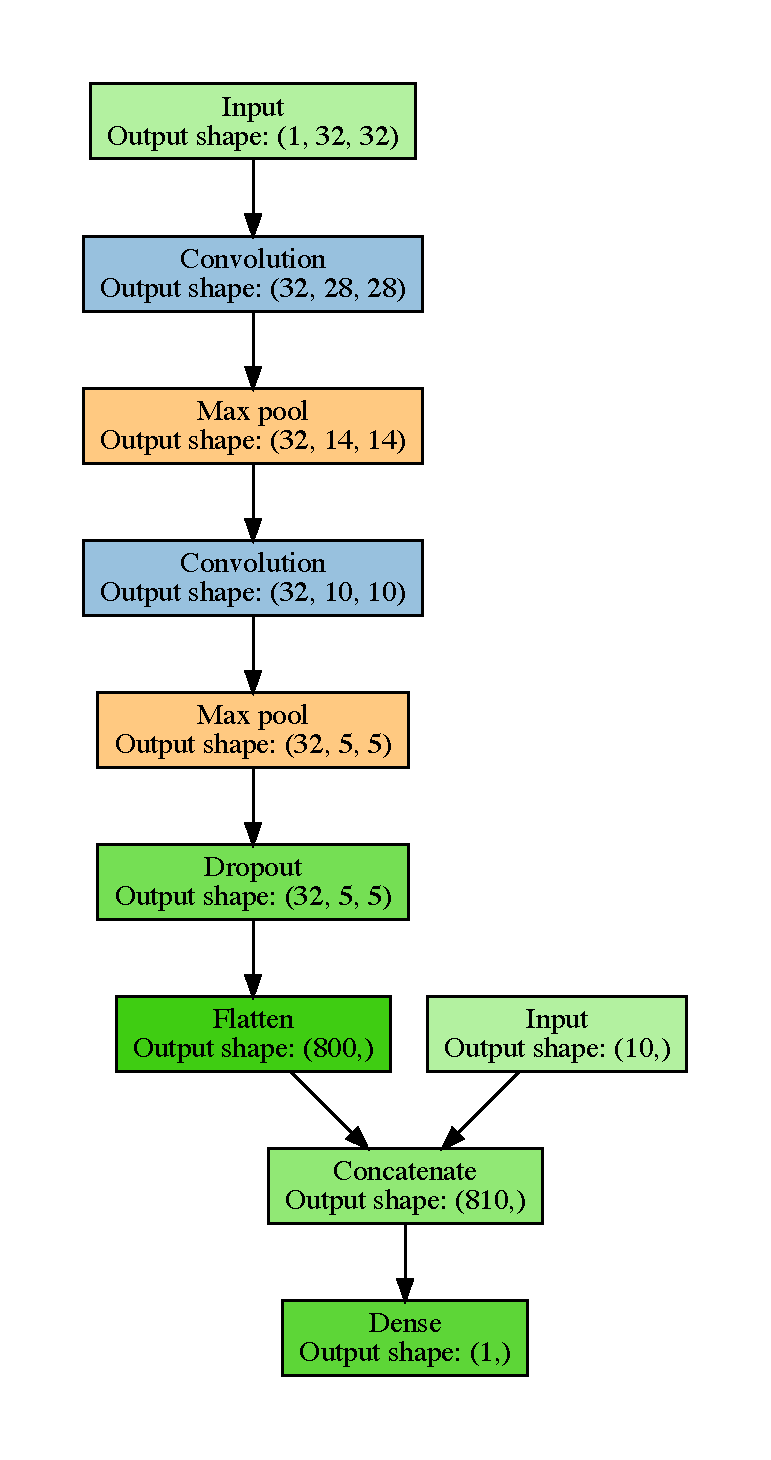
\includegraphics[height=0.9\textheight]{atlas-images/cnn_model_graph}
      \caption[Architecture of our CNN.]{\DIFaddFL{Architecture of our CNN. }{\DIFaddFL{Parenthesised numbers indicate
      the size of output layers as a tuple (width, height, depth).}} \DIFaddFL{The
      concatenate layer flattens the output of the previous layer and adds the
      10 features derived from the candidate host in SWIRE, i.e. the flux
      ratios, stellarity indices, and distance. The dropout layer randomly
      sets $25$ per cent of its inputs to zero during training to prevent
      overfitting. Diagram based on }\url{ https://github.com/dnouri/nolearn}\DIFaddFL{.}}
      \label{fig:cnn}
    \end{figure}

    \DIFadd{CNNs have recently produced good results on large image-based datasets in
    astronomy \mbox{%DIFAUXCMD
\citep[e.g.]{lukic18compact, dieleman15cnn}}\hspace{0pt}%DIFAUXCMD
. We employed
    only a simple CNN model in }\autoref{cha:cross-id} \DIFadd{as a proof of concept that CNNs may
    be used for class probability prediction on radio images. The model
    architecture we used is shown in }\autoref{fig:cnn}\DIFadd{.
}

  \subsection{\DIFadd{Random forests}}
  \label{sec:atlas-random-forests}

    \DIFadd{Random forests are an ensemble of decision
    trees~\mbox{%DIFAUXCMD
\citep{breiman01random-forest}}\hspace{0pt}%DIFAUXCMD
. They consider multiple subsamples of
    the training set, where each subsample is sampled with replacement from
    the training set. For each subsample a decision tree classifier is
    constructed by repeatedly making axis-parallel splits based on individual
    features. In a random forest the split decision is taken based on a random
    subset of features. To classify a new data point, the random forest takes
    the weighted average of all classifications produced by each decision
    tree. }{\DIFadd{In }\autoref{cha:cross-id} \DIFadd{we used the }\texttt{\DIFadd{scikit-learn}} \DIFadd{\mbox{%DIFAUXCMD
\citep{pedregosa11sklearn}
    }\hspace{0pt}%DIFAUXCMD
implementation of random forests with 10 trees, the information entropy
    split criterion, a minimum leaf size of 45, and balanced classes}}\DIFadd{.
}

\section{\DIFadd{Accuracy tables}}\label{sec:atlas-xid-accuracies}

  \DIFadd{This section contains tables of accuracy for our cross-identification method applied to CDFS and
  ELAIS-S1. In }\autoref{tab:cdfs-ba} \DIFadd{and }\autoref{tab:elais-ba} \DIFadd{we list the
  balanced accuracies of our }\autoref{cha:cross-id} \DIFadd{classifiers on the cross-identification task for CDFS
  and ELAIS-S1 respectively, averaged over each set of training quadrants. In
  }\autoref{tab:cdfs-acc} \DIFadd{and }\autoref{tab:elais-acc} \DIFadd{we list the balanced
  accuracies of classifiers on the cross-identification task for CDFS and
  ELAIS-S1 respectively, averaged over each set of training quadrants.
}

  \begin{table*}
    \caption[Balanced accuracies for different binary classification models on CDFS.]{\DIFaddFL{Balanced accuracies for different binary classification models trained and tested on SWIRE objects in CDFS.
    The `Labeller' column states what set of training labels
    were used to train the classifier, and the `Classifier' column states what
    classification model was used. `CNN' is a convolutional neural network,
    `LR' is logistic regression and `RF' is random forests. Accuracies are evaluated against the expert
    label set derived from \mbox{%DIFAUXCMD
\citet{norris06}}\hspace{0pt}%DIFAUXCMD
. The standard deviation of balanced accuracies evaluated across the four quadrants of
    CDFS (}\autoref{fig:quadrants}\DIFaddFL{) is also shown. The `compact' set refers to SWIRE
    objects within $1'$ of a compact radio component, the `resolved' set refers to
    SWIRE objects within $1'$ of a resolved radio component, and `all' is the union of these sets.}}
    \label{tab:cdfs-ba}
    \small\centering
    \begingroup
    \setlength{\tabcolsep}{8pt} %DIF >  Default value: 6pt
    \begin{tabular}{ccccc}
    \hline\hline
    \DIFaddFL{Labeller }& \DIFaddFL{Classifier }& \DIFaddFL{Mean `Compact' }& \DIFaddFL{Mean `Resolved' }& \DIFaddFL{Mean `All'}\\
     &  & \DIFaddFL{accuracy }& \DIFaddFL{accuracy }& \DIFaddFL{accuracy}\\
     &  & \DIFaddFL{(per cent) }& \DIFaddFL{(per cent) }& \DIFaddFL{(per cent)}\\
    \hline
    \DIFaddFL{Norris }& \DIFaddFL{LR }& \DIFaddFL{$91.5 \pm 1.0$ }& \DIFaddFL{$93.2 \pm 1.0$ }& \DIFaddFL{$93.0 \pm 1.2$}\\
     & \DIFaddFL{CNN }& \DIFaddFL{$92.6 \pm 0.7$ }& \DIFaddFL{$91.2 \pm 0.5$ }& \DIFaddFL{$92.0 \pm 0.6$}\\
     & \DIFaddFL{RF }& \DIFaddFL{$96.7 \pm 1.5$ }& \DIFaddFL{$91.0 \pm 4.5$ }& \DIFaddFL{$96.0 \pm 2.5$}\\
    \DIFaddFL{RGZ }& \DIFaddFL{LR }& \DIFaddFL{$89.5 \pm 0.8$ }& \DIFaddFL{$90.5 \pm 1.7$ }& \DIFaddFL{$90.2 \pm 0.8$}\\
     & \DIFaddFL{CNN }& \DIFaddFL{$89.4 \pm 0.6$ }& \DIFaddFL{$89.6 \pm 1.3$ }& \DIFaddFL{$89.4 \pm 0.5$}\\
     & \DIFaddFL{RF }& \DIFaddFL{$94.5 \pm 0.2$ }& \DIFaddFL{$95.8 \pm 0.4$ }& \DIFaddFL{$94.7 \pm 0.3$}\\
    \hline\hline
    \end{tabular}
    \endgroup
  \end{table*}

  \begin{table*}
    \caption[Balanced accuracies for different binary classification models on ELAIS-S1.]{\DIFaddFL{Balanced accuracies for different binary classification models trained on SWIRE objects
    in CDFS and tested on SWIRE objects in ELAIS-S1. Columns and abbreviations are as in }\autoref{tab:cdfs-ba}\DIFaddFL{. Accuracies are evaluated against the expert
    label set derived from \mbox{%DIFAUXCMD
\citet{middelberg08}}\hspace{0pt}%DIFAUXCMD
. The standard deviations of balanced accuracies of models trained on the four subsets of
    CDFS (}\autoref{fig:quadrants}\DIFaddFL{) are also shown.}}
    \label{tab:elais-ba}
    \small\centering
    \begingroup
    \setlength{\tabcolsep}{8pt} %DIF >  Default value: 6pt
    \begin{tabular}{ccccc}
      \hline\hline
      \DIFaddFL{Labeller }& \DIFaddFL{Classifier }& \DIFaddFL{Mean `Compact' }& \DIFaddFL{Mean `Resolved' }& \DIFaddFL{Mean `All'}\\
        &  & \DIFaddFL{accuracy }& \DIFaddFL{accuracy }& \DIFaddFL{accuracy}\\
        &  & \DIFaddFL{(per cent) }& \DIFaddFL{(per cent) }& \DIFaddFL{(per cent)}\\
      \hline
      \DIFaddFL{Norris }& \DIFaddFL{LR }& \DIFaddFL{$94.6 \pm 0.4$ }& \DIFaddFL{$93.3 \pm 2.0$ }& \DIFaddFL{$95.3 \pm 0.1$}\\
       & \DIFaddFL{CNN }& \DIFaddFL{$94.8 \pm 0.2$ }& \DIFaddFL{$92.8 \pm 0.5$ }& \DIFaddFL{$94.4 \pm 0.2$}\\
       & \DIFaddFL{RF }& \DIFaddFL{$85.9 \pm 3.8$ }& \DIFaddFL{$70.0 \pm 2.8$ }& \DIFaddFL{$86.6 \pm 3.2$}\\
      \DIFaddFL{RGZ }& \DIFaddFL{LR }& \DIFaddFL{$91.8 \pm 0.3$ }& \DIFaddFL{$91.9 \pm 0.5$ }& \DIFaddFL{$92.0 \pm 0.2$}\\
       & \DIFaddFL{CNN }& \DIFaddFL{$90.1 \pm 0.3$ }& \DIFaddFL{$91.1 \pm 0.9$ }& \DIFaddFL{$90.2 \pm 0.3$}\\
       & \DIFaddFL{RF }& \DIFaddFL{$95.1 \pm 0.1$ }& \DIFaddFL{$95.2 \pm 0.0$ }& \DIFaddFL{$95.2 \pm 0.3$}\\
      \hline\hline
    \end{tabular}
    \endgroup
  \end{table*}

  \begin{table*}
    \caption[Cross-identification accuracies for different classification
    models on CDFS.]{\DIFaddFL{Cross-identification accuracies for different classification
    models on CDFS. The `Labeller' column states what set of training labels
    were used to train the method, and the `Classifier' column states what
    classification model was used. `CNN' is a convolutional neural network,
    `LR' is logistic regression, `RF' is random forests, and `Labels' is the
    accuracy of the label set itself. `Perfect' indicates that the true labels
    of the test set were used and hence represents an upper bound on
    cross-identification accuracy with our method. `NN' is a
    nearest neighbours approach. Accuracies are evaluated against the expert
    label set, so `Norris' labels are 100 per cent accurate by definition. The
    standard deviation of accuracies evaluated across the four quadrants of
    CDFS (}\autoref{fig:quadrants}\DIFaddFL{) is also shown.}}
    \label{tab:cdfs-acc}
    \small\centering
    \begingroup
    \setlength{\tabcolsep}{8pt} %DIF >  Default value: 6pt
    \begin{tabular}{ccccc}
      \hline\hline
      \DIFaddFL{Labeller }& \DIFaddFL{Classifier }& \DIFaddFL{Mean `Compact' }& \DIFaddFL{Mean `Resolved' }& \DIFaddFL{Mean `All'}\\
       &  & \DIFaddFL{accuracy }& \DIFaddFL{accuracy }& \DIFaddFL{accuracy}\\
       &  & \DIFaddFL{(per cent) }& \DIFaddFL{(per cent) }& \DIFaddFL{(per cent)}\\
      \hline
     \DIFaddFL{---}& \DIFaddFL{NN }& \DIFaddFL{$97.2 \pm 1.7$ }& \DIFaddFL{$75.7 \pm 7.9$ }& \DIFaddFL{$93.4 \pm 0.8$}\\
     \DIFaddFL{---}& \DIFaddFL{Random }& \DIFaddFL{$97.9 \pm 2.2$ }& \DIFaddFL{$22.3 \pm 9.2$ }& \DIFaddFL{$83.2 \pm 4.7$}\\
      \DIFaddFL{Norris }& \DIFaddFL{Labels }& \DIFaddFL{$100.0 \pm 0.0$ }& \DIFaddFL{$100.0 \pm 0.0$ }& \DIFaddFL{$100.0 \pm 0.0$}\\
             & \DIFaddFL{Perfect }& \DIFaddFL{$97.9 \pm 2.2$ }& \DIFaddFL{$99.0 \pm 1.8$ }& \DIFaddFL{$98.1 \pm 1.7$}\\
             & \DIFaddFL{LR }& \DIFaddFL{$97.3 \pm 0.5$ }& \DIFaddFL{$76.0 \pm 3.2$ }& \DIFaddFL{$93.7 \pm 1.8$}\\
             & \DIFaddFL{CNN }& \DIFaddFL{$96.6 \pm 0.9$ }& \DIFaddFL{$74.3 \pm 12.3$ }& \DIFaddFL{$93.5 \pm 0.5$}\\
             & \DIFaddFL{RF }& \DIFaddFL{$96.1 \pm 1.4$ }& \DIFaddFL{$75.8 \pm 6.7$ }& \DIFaddFL{$93.8 \pm 2.0$}\\
      \DIFaddFL{RGZ }& \DIFaddFL{Labels }& \DIFaddFL{$53.1 \pm 8.5$ }& \DIFaddFL{$56.7 \pm 5.9$ }& \DIFaddFL{$54.4 \pm 5.9$}\\
          & \DIFaddFL{LR }& \DIFaddFL{$97.3 \pm 1.9$ }& \DIFaddFL{$74.5 \pm 5.1$ }& \DIFaddFL{$93.6 \pm 1.7$}\\
          & \DIFaddFL{CNN }& \DIFaddFL{$85.4 \pm 2.6$ }& \DIFaddFL{$68.1 \pm 9.2$ }& \DIFaddFL{$92.4 \pm 1.1$}\\
          & \DIFaddFL{RF }& \DIFaddFL{$97.5 \pm 0.9$ }& \DIFaddFL{$74.3 \pm 7.9$ }& \DIFaddFL{$93.7 \pm 1.5$}\\
      \hline\hline
    \end{tabular}
    \endgroup
  \end{table*}

  \begin{table*}
    \caption[Cross-identification accuracies for different classification
    models on ELAIS-S1.]{\DIFaddFL{Cross-identification accuracies for different classification
    models on ELAIS-S1. Columns and abbreviations are as in
    }\autoref{tab:cdfs-acc}\DIFaddFL{. Accuracies are evaluated against the expert label
    set derived from \mbox{%DIFAUXCMD
\citet{middelberg08} }\hspace{0pt}%DIFAUXCMD
cross-identifications. The standard
    deviation of accuracies evaluated across models trained on the four
    quadrants of CDFS (}\autoref{fig:quadrants}\DIFaddFL{) is also shown.}}
    \label{tab:elais-acc}
    \small\centering
    \begingroup
    \setlength{\tabcolsep}{8pt} %DIF >  Default value: 6pt
    \begin{tabular}{ccccc}
      \hline\hline
      \DIFaddFL{Labeller }& \DIFaddFL{Classifier }& \DIFaddFL{Mean `Compact' }& \DIFaddFL{Mean `Resolved' }& \DIFaddFL{Mean `All'}\\
       &  & \DIFaddFL{accuracy }& \DIFaddFL{accuracy }& \DIFaddFL{accuracy}\\
       &  & \DIFaddFL{(per cent) }& \DIFaddFL{(per cent) }& \DIFaddFL{(per cent)}\\
      \hline
     \DIFaddFL{---}& \DIFaddFL{NN }& \DIFaddFL{$95.5 \pm 0.0$ }& \DIFaddFL{$92.8 \pm 0.0$ }& \DIFaddFL{$95.5 \pm 0.0$}\\
     \DIFaddFL{---}& \DIFaddFL{Random }& \DIFaddFL{$61.9 \pm 1.1$ }& \DIFaddFL{$26.6 \pm 2.1$ }& \DIFaddFL{$61.9 \pm 1.1$}\\
      \DIFaddFL{Middelberg }& \DIFaddFL{Perfect }& \DIFaddFL{$99.6 \pm 0.0$ }& \DIFaddFL{$99.8 \pm 0.0$ }& \DIFaddFL{$99.6 \pm 0.0$}\\
      \DIFaddFL{Norris }& \DIFaddFL{LR }& \DIFaddFL{$89.0 \pm 1.1$ }& \DIFaddFL{$89.7 \pm 1.8$ }& \DIFaddFL{$94.4 \pm 0.9$}\\
             & \DIFaddFL{CNN }& \DIFaddFL{$89.7 \pm 0.3$ }& \DIFaddFL{$89.4 \pm 1.4$ }& \DIFaddFL{$94.3 \pm 0.7$}\\
             & \DIFaddFL{RF }& \DIFaddFL{$83.8 \pm 5.6$ }& \DIFaddFL{$82.3 \pm 4.1$ }& \DIFaddFL{$90.6 \pm 2.1$}\\
      \DIFaddFL{RGZ }& \DIFaddFL{LR }& \DIFaddFL{$90.5 \pm 1.0$ }& \DIFaddFL{$92.7 \pm 0.2$ }& \DIFaddFL{$95.9 \pm 0.1$}\\
          & \DIFaddFL{CNN }& \DIFaddFL{$84.6 \pm 0.6$ }& \DIFaddFL{$84.6 \pm 0.6$ }& \DIFaddFL{$91.8 \pm 0.3$}\\
          & \DIFaddFL{RF }& \DIFaddFL{$91.3 \pm 1.0$ }& \DIFaddFL{$90.3 \pm 2.4$ }& \DIFaddFL{$94.7 \pm 1.2$}\\
      \hline\hline
    \end{tabular}
    \endgroup
  \end{table*}

\section{\DIFadd{SWIRE object scores}}\label{sec:atlas-xid-scores}

  \DIFadd{This appendix contains scores predicted by our }\autoref{cha:cross-id} \DIFadd{binary classifiers for each
  SWIRE object within $1'$ of a radio component in CDFS and ELAIS-S1. Scores
  for SWIRE~CDFS objects are shown in }\autoref{tab:cdfs-scores} \DIFadd{and scores for
  SWIRE~ELAIS-S1 are shown in }\autoref{tab:elais-scores}\DIFadd{. For CDFS, the score
  for an object in a quadrant is predicted by binary classifiers trained on
  all other quadrants. For ELAIS-S1, we show the scores predicted by binary
  classifiers trained on each CDFS quadrant. Note that these scores have
  }\emph{\DIFadd{not}} \DIFadd{been weighted by Gaussians. These are partial tables, and the full tables are available online at the }\emph{\DIFadd{Monthly Notices of the Royal Astronomical Society}} \DIFadd{website}\footnote{\url{https://doi.org/10.1093/mnras/sty1308}}\DIFadd{.
}

  \DIFadd{The columns of the score tables are defined as follows:
  }\begin{itemize}
    \item \emph{\DIFadd{SWIRE}}\DIFadd{---SWIRE designation for candidate host galaxy.
    }\item \emph{\DIFadd{RA}}\DIFadd{---Right ascension (J2000).
    }\item \emph{\DIFadd{Dec}}\DIFadd{---Declination (J2000).
    }\item \emph{\DIFadd{Expert host}}\DIFadd{---Whether the candidate host galaxy is a host galaxy according to \mbox{%DIFAUXCMD
\citet{norris06} }\hspace{0pt}%DIFAUXCMD
or \mbox{%DIFAUXCMD
\citet{middelberg08} }\hspace{0pt}%DIFAUXCMD
cross-identifications of CDFS and ELAIS-S1 respectively.
    }\item \emph{\DIFadd{RGZ host}}\DIFadd{---Whether the candidate host galaxy is a host galaxy according to Radio Galaxy Zoo cross-identifications \mbox{%DIFAUXCMD
\citep{wong21rgz}}\hspace{0pt}%DIFAUXCMD
. This is always `no' for ELAIS-S1 objects.
    }\item \emph{\DIFadd{$C$/$L$/$D$}}\DIFadd{---Score assigned by binary classifier $C$ trained on label set $L$ of $D$ candidate host galaxies. $C$ may be `CNN', `LR' or `RF' for CNN, logistic regression, or random forests respectively. $L$ may be `Norris' or `RGZ' for expert and Radio Galaxy Zoo labels respectively. $D$ may be `All', `Compact', or `Resolved' for each respective subset defined in }\autoref{sec:atlas-xid-experimental-setup}\DIFadd{.
  }\end{itemize}

  \begin{sidewaystable}
    \caption[Scores output by our trained classifiers for SWIRE~CDFS candidate host galaxies.]{\DIFadd{Scores output by our trained classifiers for SWIRE~CDFS candidate host galaxies. Columns are defined in }\aref{sec:atlas-xid-scores}\DIFadd{. Full table electronic.}}
    \label{tab:cdfs-scores}
    \small\centering
    \begin{tabular}{ccccccccccc}
      \hline\hline
\DIFadd{SWIRE }& \DIFadd{RA }& \DIFadd{Dec }& \DIFadd{Expert }& \DIFadd{RGZ }& \multicolumn{6}{c}{CNN}\\
& & & \DIFadd{host }& \DIFadd{host }& \multicolumn{3}{c}{Norris} & \multicolumn{3}{c}{RGZ}\\
& & & & & \DIFadd{All }& \DIFadd{Compact }& \DIFadd{Resolved }& \DIFadd{All }& \DIFadd{Compact }& \DIFadd{Resolved}\\
      \hline
\DIFadd{J032603.15-284708.5 }& \DIFadd{51.5132 }& \DIFadd{-28.7857 }& \DIFadd{yes }& \DIFadd{no }& \DIFadd{0.5838 }& \DIFadd{0.4697 }& \DIFadd{0.4848 }& \DIFadd{0.3754 }& \DIFadd{0.3881 }& \DIFadd{0.3404 }\\
\DIFadd{J032603.39-284010.1 }& \DIFadd{51.5142 }& \DIFadd{-28.6695 }& \DIFadd{no }& \DIFadd{no }& \DIFadd{0.0373 }& \DIFadd{0.5814 }& \DIFadd{0.4878 }& \DIFadd{0.7896 }& \DIFadd{0.7616 }& \DIFadd{0.4668 }\\
\DIFadd{J032603.44-284210.1 }& \DIFadd{51.5144 }& \DIFadd{-28.7028 }& \DIFadd{no }& \DIFadd{no }& \DIFadd{0.0232 }& \DIFadd{0.4891 }& \DIFadd{0.5101 }& \DIFadd{0.4319 }& \DIFadd{0.4298 }& \DIFadd{0.3474 }\\
\DIFadd{J032603.44-284222.2 }& \DIFadd{51.5143 }& \DIFadd{-28.7062 }& \DIFadd{no }& \DIFadd{no }& \DIFadd{0.0006 }& \DIFadd{0.4164 }& \DIFadd{0.5216 }& \DIFadd{0.0400 }& \DIFadd{0.0444 }& \DIFadd{0.0276 }\\
\DIFadd{J032603.45-284748.4 }& \DIFadd{51.5144 }& \DIFadd{-28.7968 }& \DIFadd{no }& \DIFadd{no }& \DIFadd{0.0014 }& \DIFadd{0.4914 }& \DIFadd{0.4865 }& \DIFadd{0.1904 }& \DIFadd{0.1895 }& \DIFadd{0.1467 }\\
\DIFadd{J032603.50-284637.0 }& \DIFadd{51.5146 }& \DIFadd{-28.7770 }& \DIFadd{no }& \DIFadd{no }& \DIFadd{0.0074 }& \DIFadd{0.4144 }& \DIFadd{0.5382 }& \DIFadd{0.1418 }& \DIFadd{0.1515 }& \DIFadd{0.1166 }\\
\DIFadd{J032603.60-284627.4 }& \DIFadd{51.5150 }& \DIFadd{-28.7743 }& \DIFadd{no }& \DIFadd{no }& \DIFadd{0.0012 }& \DIFadd{0.4578 }& \DIFadd{0.5165 }& \DIFadd{0.0850 }& \DIFadd{0.0904 }& \DIFadd{0.0484 }\\
\DIFadd{J032603.63-283840.5 }& \DIFadd{51.5151 }& \DIFadd{-28.6446 }& \DIFadd{no }& \DIFadd{no }& \DIFadd{0.0021 }& \DIFadd{0.4153 }& \DIFadd{0.5577 }& \DIFadd{0.1678 }& \DIFadd{0.1746 }& \DIFadd{0.1323 }\\
\DIFadd{J032603.66-283822.8 }& \DIFadd{51.5153 }& \DIFadd{-28.6397 }& \DIFadd{no }& \DIFadd{no }& \DIFadd{0.0001 }& \DIFadd{0.4752 }& \DIFadd{0.5009 }& \DIFadd{0.0864 }& \DIFadd{0.0861 }& \DIFadd{0.0613 }\\
\DIFadd{J032603.75-284014.1 }& \DIFadd{51.5156 }& \DIFadd{-28.6706 }& \DIFadd{no }& \DIFadd{no }& \DIFadd{0.0547 }& \DIFadd{0.3408 }& \DIFadd{0.5388 }& \DIFadd{0.4889 }& \DIFadd{0.5242 }& \DIFadd{0.7301 }\\
      \hline\hline
    \end{tabular}\\
    \begin{tabular}{cccccccccccc}
      \hline\hline
\multicolumn{6}{c}{LR} & \multicolumn{6}{c}{RF} \\
\multicolumn{3}{c}{Norris} & \multicolumn{3}{c}{RGZ} & \multicolumn{3}{c}{Norris} & \multicolumn{3}{c}{RGZ} \\
\DIFadd{All }& \DIFadd{Compact }& \DIFadd{Resolved }& \DIFadd{All }& \DIFadd{Compact }& \DIFadd{Resolved }& \DIFadd{All }& \DIFadd{Compact }& \DIFadd{Resolved }& \DIFadd{All }& \DIFadd{Compact }& \DIFadd{Resolved }\\
      \hline
\DIFadd{0.2489 }& \DIFadd{0.0009 }& \DIFadd{0.1557 }& \DIFadd{0.2939 }& \DIFadd{0.0007 }& \DIFadd{0.1174 }& \DIFadd{0.8922 }& \DIFadd{0.8018 }& \DIFadd{0.8732 }& \DIFadd{0.7167 }& \DIFadd{0.6599 }& \DIFadd{0.7801 }\\
\DIFadd{0.0183 }& \DIFadd{0.1646 }& \DIFadd{0.1480 }& \DIFadd{0.7637 }& \DIFadd{0.7065 }& \DIFadd{0.6070 }& \DIFadd{0.0000 }& \DIFadd{0.0000 }& \DIFadd{0.0000 }& \DIFadd{0.1629 }& \DIFadd{0.0519 }& \DIFadd{0.1275 }\\
\DIFadd{0.0155 }& \DIFadd{0.0164 }& \DIFadd{0.0815 }& \DIFadd{0.3714 }& \DIFadd{0.5626 }& \DIFadd{0.2488 }& \DIFadd{0.0000 }& \DIFadd{0.0734 }& \DIFadd{0.0000 }& \DIFadd{0.1315 }& \DIFadd{0.2116 }& \DIFadd{0.4150 }\\
\DIFadd{0.0005 }& \DIFadd{0.0006 }& \DIFadd{0.0175 }& \DIFadd{0.0460 }& \DIFadd{0.0810 }& \DIFadd{0.0299 }& \DIFadd{0.2656 }& \DIFadd{0.1418 }& \DIFadd{0.0000 }& \DIFadd{0.7631 }& \DIFadd{0.8166 }& \DIFadd{0.5378 }\\
\DIFadd{0.0013 }& \DIFadd{0.0037 }& \DIFadd{0.0160 }& \DIFadd{0.1792 }& \DIFadd{0.0663 }& \DIFadd{0.1821 }& \DIFadd{0.0000 }& \DIFadd{0.0000 }& \DIFadd{0.0000 }& \DIFadd{0.0255 }& \DIFadd{0.0000 }& \DIFadd{0.0000 }\\
\DIFadd{0.0047 }& \DIFadd{0.0010 }& \DIFadd{0.0337 }& \DIFadd{0.1284 }& \DIFadd{0.2198 }& \DIFadd{0.0694 }& \DIFadd{0.0720 }& \DIFadd{0.0000 }& \DIFadd{0.0000 }& \DIFadd{0.6240 }& \DIFadd{0.6681 }& \DIFadd{0.6704 }\\
\DIFadd{0.0008 }& \DIFadd{0.0006 }& \DIFadd{0.0374 }& \DIFadd{0.1053 }& \DIFadd{0.1424 }& \DIFadd{0.0807 }& \DIFadd{0.1231 }& \DIFadd{0.0876 }& \DIFadd{0.0000 }& \DIFadd{0.8517 }& \DIFadd{0.7532 }& \DIFadd{0.7019 }\\
\DIFadd{0.0021 }& \DIFadd{0.0073 }& \DIFadd{0.0386 }& \DIFadd{0.1482 }& \DIFadd{0.0403 }& \DIFadd{0.1210 }& \DIFadd{0.0000 }& \DIFadd{0.0532 }& \DIFadd{0.0000 }& \DIFadd{0.0000 }& \DIFadd{0.0302 }& \DIFadd{0.0000 }\\
\DIFadd{0.0001 }& \DIFadd{0.0004 }& \DIFadd{0.0038 }& \DIFadd{0.0854 }& \DIFadd{0.0447 }& \DIFadd{0.0514 }& \DIFadd{0.0000 }& \DIFadd{0.0000 }& \DIFadd{0.0000 }& \DIFadd{0.0000 }& \DIFadd{0.0000 }& \DIFadd{0.0000 }\\
\DIFadd{0.0542 }& \DIFadd{0.2712 }& \DIFadd{0.2318 }& \DIFadd{0.5026 }& \DIFadd{0.5631 }& \DIFadd{0.5032 }& \DIFadd{0.0595 }& \DIFadd{0.0545 }& \DIFadd{0.0000 }& \DIFadd{0.4289 }& \DIFadd{0.0789 }& \DIFadd{0.1420 }\\
      \hline\hline
    \end{tabular}
  \end{sidewaystable}

  \begin{sidewaystable}
    \caption[Scores output by our trained classifiers for SWIRE~ELAIS-S1 candidate host galaxies.]{\DIFadd{Scores output by our trained classifiers for SWIRE~ELAIS-S1 candidate host galaxies. Columns are defined in }\aref{sec:atlas-xid-scores}\DIFadd{. Full table electronic.}}
    \label{tab:elais-scores}
    \small\centering
    \begin{tabular}{ccccccccccc}
      \hline\hline
\DIFadd{SWIRE }& \DIFadd{RA }& \DIFadd{Dec }& \DIFadd{Expert }& \DIFadd{RGZ }& \multicolumn{6}{c}{CNN} \\
 & & & \DIFadd{host }& \DIFadd{host }& \multicolumn{3}{c}{Norris} & \multicolumn{3}{c}{RGZ} \\
 & & & & & \DIFadd{All }& \DIFadd{Compact }& \DIFadd{Resolved }& \DIFadd{All }& \DIFadd{Compact }& \DIFadd{Resolved }\\
      \hline
\DIFadd{J002925.73-440256.2 }& \DIFadd{7.3572 }& \DIFadd{-44.0490 }& \DIFadd{yes }& \DIFadd{no }& \DIFadd{0.9537 }& \DIFadd{0.8638 }& \DIFadd{0.5552 }& \DIFadd{0.9195 }& \DIFadd{0.9037 }& \DIFadd{0.9371}\\
\DIFadd{J002926.14-440249.0 }& \DIFadd{7.3590 }& \DIFadd{-44.0470 }& \DIFadd{no }& \DIFadd{no }& \DIFadd{0.7361 }& \DIFadd{0.8752 }& \DIFadd{0.5640 }& \DIFadd{0.7740 }& \DIFadd{0.7474 }& \DIFadd{0.7952}\\
\DIFadd{J002926.52-440247.0 }& \DIFadd{7.3605 }& \DIFadd{-44.0464 }& \DIFadd{no }& \DIFadd{no }& \DIFadd{0.3390 }& \DIFadd{0.8338 }& \DIFadd{0.5556 }& \DIFadd{0.7275 }& \DIFadd{0.6894 }& \DIFadd{0.7197}\\
\DIFadd{J002926.63-440301.1 }& \DIFadd{7.3610 }& \DIFadd{-44.0503 }& \DIFadd{no }& \DIFadd{no }& \DIFadd{0.2108 }& \DIFadd{0.8251 }& \DIFadd{0.5623 }& \DIFadd{0.3434 }& \DIFadd{0.3306 }& \DIFadd{0.3292}\\
\DIFadd{J002927.13-440232.6 }& \DIFadd{7.3631 }& \DIFadd{-44.0424 }& \DIFadd{no }& \DIFadd{no }& \DIFadd{0.0339 }& \DIFadd{0.8479 }& \DIFadd{0.5669 }& \DIFadd{0.5853 }& \DIFadd{0.5148 }& \DIFadd{0.5159}\\
\DIFadd{J002927.28-440245.3 }& \DIFadd{7.3637 }& \DIFadd{-44.0459 }& \DIFadd{no }& \DIFadd{no }& \DIFadd{0.0406 }& \DIFadd{0.8345 }& \DIFadd{0.5540 }& \DIFadd{0.2702 }& \DIFadd{0.2340 }& \DIFadd{0.2133}\\
\DIFadd{J002927.44-440238.5 }& \DIFadd{7.3644 }& \DIFadd{-44.0440 }& \DIFadd{no }& \DIFadd{no }& \DIFadd{0.0116 }& \DIFadd{0.8267 }& \DIFadd{0.5746 }& \DIFadd{0.2228 }& \DIFadd{0.2182 }& \DIFadd{0.2028}\\
\DIFadd{J002928.08-440230.3 }& \DIFadd{7.3670 }& \DIFadd{-44.0418 }& \DIFadd{no }& \DIFadd{no }& \DIFadd{0.0024 }& \DIFadd{0.8626 }& \DIFadd{0.5791 }& \DIFadd{0.2297 }& \DIFadd{0.1963 }& \DIFadd{0.1549}\\
\DIFadd{J002928.11-440312.7 }& \DIFadd{7.3671 }& \DIFadd{-44.0535 }& \DIFadd{no }& \DIFadd{no }& \DIFadd{0.0011 }& \DIFadd{0.8159 }& \DIFadd{0.5514 }& \DIFadd{0.0377 }& \DIFadd{0.0384 }& \DIFadd{0.0271}\\
\DIFadd{J002928.80-440306.8 }& \DIFadd{7.3700 }& \DIFadd{-44.0519 }& \DIFadd{no }& \DIFadd{no }& \DIFadd{0.0003 }& \DIFadd{0.8405 }& \DIFadd{0.5668 }& \DIFadd{0.0236 }& \DIFadd{0.0226 }& \DIFadd{0.0136}\\
      \hline\hline
    \end{tabular}\\
    \begin{tabular}{cccccccccccc}
      \hline\hline
\multicolumn{6}{c}{LR} & \multicolumn{6}{c}{RF} \\
\multicolumn{3}{c}{LR} & \multicolumn{3}{c}{LR} & \multicolumn{3}{c}{RF} & \multicolumn{3}{c}{RF} \\
\DIFadd{All }& \DIFadd{Compact }& \DIFadd{Resolved }& \DIFadd{All }& \DIFadd{Compact }& \DIFadd{Resolved }& \DIFadd{All }& \DIFadd{Compact }& \DIFadd{Resolved }& \DIFadd{All }& \DIFadd{Compact }& \DIFadd{Resolved }\\
      \hline
\DIFadd{0.9722 }& \DIFadd{0.9955 }& \DIFadd{0.8769 }& \DIFadd{0.9933 }& \DIFadd{0.9934 }& \DIFadd{0.9658 }& \DIFadd{0.8824 }& \DIFadd{0.9664 }& \DIFadd{0.7950 }& \DIFadd{0.8078 }& \DIFadd{0.9227 }& \DIFadd{0.7677 }\\
\DIFadd{0.4669 }& \DIFadd{0.0111 }& \DIFadd{0.4249 }& \DIFadd{0.3926 }& \DIFadd{0.2220 }& \DIFadd{0.5947 }& \DIFadd{0.2077 }& \DIFadd{0.0000 }& \DIFadd{0.1613 }& \DIFadd{0.1876 }& \DIFadd{0.0852 }& \DIFadd{0.4546 }\\
\DIFadd{0.2264 }& \DIFadd{0.0254 }& \DIFadd{0.2389 }& \DIFadd{0.6275 }& \DIFadd{0.3033 }& \DIFadd{0.6812 }& \DIFadd{0.1347 }& \DIFadd{0.0857 }& \DIFadd{0.0399 }& \DIFadd{0.3582 }& \DIFadd{0.4854 }& \DIFadd{0.5347 }\\
\DIFadd{0.0603 }& \DIFadd{0.0007 }& \DIFadd{0.0734 }& \DIFadd{0.0688 }& \DIFadd{0.0141 }& \DIFadd{0.1581 }& \DIFadd{0.0917 }& \DIFadd{0.0000 }& \DIFadd{0.0399 }& \DIFadd{0.2846 }& \DIFadd{0.1245 }& \DIFadd{0.2833 }\\
\DIFadd{0.0248 }& \DIFadd{0.0334 }& \DIFadd{0.0301 }& \DIFadd{0.5735 }& \DIFadd{0.5065 }& \DIFadd{0.5265 }& \DIFadd{0.1977 }& \DIFadd{0.1507 }& \DIFadd{0.0000 }& \DIFadd{0.3334 }& \DIFadd{0.6593 }& \DIFadd{0.3995 }\\
\DIFadd{0.0173 }& \DIFadd{0.0016 }& \DIFadd{0.0359 }& \DIFadd{0.1056 }& \DIFadd{0.0492 }& \DIFadd{0.1456 }& \DIFadd{0.0000 }& \DIFadd{0.0000 }& \DIFadd{0.0000 }& \DIFadd{0.0000 }& \DIFadd{0.0000 }& \DIFadd{0.0287 }\\
\DIFadd{0.0064 }& \DIFadd{0.0049 }& \DIFadd{0.0187 }& \DIFadd{0.1981 }& \DIFadd{0.1534 }& \DIFadd{0.1493 }& \DIFadd{0.0000 }& \DIFadd{0.0000 }& \DIFadd{0.0000 }& \DIFadd{0.1565 }& \DIFadd{0.1634 }& \DIFadd{0.1284 }\\
\DIFadd{0.0020 }& \DIFadd{0.0005 }& \DIFadd{0.0239 }& \DIFadd{0.1337 }& \DIFadd{0.1001 }& \DIFadd{0.1310 }& \DIFadd{0.0000 }& \DIFadd{0.0000 }& \DIFadd{0.0358 }& \DIFadd{0.0000 }& \DIFadd{0.0000 }& \DIFadd{0.0190 }\\
\DIFadd{0.0008 }& \DIFadd{0.0013 }& \DIFadd{0.0119 }& \DIFadd{0.0280 }& \DIFadd{0.0361 }& \DIFadd{0.0205 }& \DIFadd{0.1171 }& \DIFadd{0.0000 }& \DIFadd{0.0000 }& \DIFadd{0.0873 }& \DIFadd{0.0383 }& \DIFadd{0.0000 }\\
\DIFadd{0.0004 }& \DIFadd{0.0014 }& \DIFadd{0.0095 }& \DIFadd{0.0339 }& \DIFadd{0.0408 }& \DIFadd{0.0136 }& \DIFadd{0.0000 }& \DIFadd{0.0000 }& \DIFadd{0.0000 }& \DIFadd{0.1114 }& \DIFadd{0.1480 }& \DIFadd{0.1584 }\\
      \hline\hline
    \end{tabular}
  \end{sidewaystable}

\section{\DIFadd{ATLAS component cross-identifications}}\label{sec:atlas-xid-xids}

  \DIFadd{This section contains cross-identifications predicted by our cross-identification method for each
  ATLAS radio component in CDFS and ELAIS-S1. Cross-identifications for
  ATLAS~CDFS components are shown in }\autoref{tab:cdfs-xids} \DIFadd{and
  cross-identifications for ATLAS~ELAIS-S1 are shown in
  }\autoref{tab:elais-xids}\DIFadd{. For CDFS, the cross-identification for a component
  in a quadrant is predicted using our method with binary classifiers trained
  on all other quadrants. For ELAIS-S1, we show the cross-identifications
  predicted by our method using binary classifiers trained on each CDFS
  quadrant. For CDFS, we also show the Radio Galaxy Zoo consensus, which is a
  proxy for the difficulty of cross-identifying a component \mbox{%DIFAUXCMD
\citep{wong21rgz}}\hspace{0pt}%DIFAUXCMD
. These are partial tables, and the full tables are available online at the }\emph{\DIFadd{Monthly Notices of the Royal Astronomical Society}} \DIFadd{website}\footnote{\url{https://doi.org/10.1093/mnras/sty1308}}\DIFadd{.
}

  \DIFadd{The columns of the cross-identification tables are defined as follows:
  }\begin{itemize}
    \item \emph{\DIFadd{ATLAS}}\DIFadd{---ATLAS designation for radio component.
    }\item \emph{\DIFadd{RA}}\DIFadd{---Right ascension of radio component (J2000).
    }\item \emph{\DIFadd{Dec}}\DIFadd{---Declination of radio component (J2000).
    }\item \emph{\DIFadd{CID}}\DIFadd{---Radio Galaxy Zoo component ID.
    }\item \emph{\DIFadd{Zooniverse ID}}\DIFadd{---Radio Galaxy Zoo Zooniverse ID.
    }\item \emph{\DIFadd{Norris/Middelberg}}\DIFadd{---Designation of SWIRE cross-identification from \mbox{%DIFAUXCMD
\citet{norris06} }\hspace{0pt}%DIFAUXCMD
or \mbox{%DIFAUXCMD
\citet{middelberg08} }\hspace{0pt}%DIFAUXCMD
for CDFS and ELAIS-S1 respectively.
    }\item \emph{\DIFadd{Norris/Middelberg RA}}\DIFadd{---Right ascension of SWIRE cross-identification from \mbox{%DIFAUXCMD
\citet{norris06} }\hspace{0pt}%DIFAUXCMD
or \mbox{%DIFAUXCMD
\citet{middelberg08} }\hspace{0pt}%DIFAUXCMD
for CDFS and ELAIS-S1 respectively.
    }\item \emph{\DIFadd{Norris/Middelberg Dec}}\DIFadd{---Right ascension of SWIRE cross-identification from \mbox{%DIFAUXCMD
\citet{norris06} }\hspace{0pt}%DIFAUXCMD
or \mbox{%DIFAUXCMD
\citet{middelberg08} }\hspace{0pt}%DIFAUXCMD
for CDFS and ELAIS-S1 respectively.
    }\item \emph{\DIFadd{RGZ}}\DIFadd{---Designation of SWIRE cross-identification from Radio Galaxy Zoo \mbox{%DIFAUXCMD
\citep{wong21rgz}}\hspace{0pt}%DIFAUXCMD
.
    }\item \emph{\DIFadd{RGZ RA}}\DIFadd{---Right ascension of SWIRE cross-identification from Radio Galaxy Zoo \mbox{%DIFAUXCMD
\citep{wong21rgz}}\hspace{0pt}%DIFAUXCMD
.
    }\item \emph{\DIFadd{RGZ Dec}}\DIFadd{---Right ascension of SWIRE cross-identification from Radio Galaxy Zoo \mbox{%DIFAUXCMD
\citep{wong21rgz}}\hspace{0pt}%DIFAUXCMD
.
    }\item \emph{\DIFadd{RGZ radio consensus}}\DIFadd{---Percentage agreement of Radio Galaxy Zoo volunteers on the radio component configuration.
    }\item \emph{\DIFadd{RGZ IR consensus}}\DIFadd{---Percentage agreement of Radio Galaxy Zoo volunteers on the host galaxy of this radio component.
    }\item \emph{\DIFadd{$C$ / $L$ / $D$}}\DIFadd{---Designation of SWIRE cross-identification made by our method using classification model $C$ trained on label set $L$ of $D$ candidate host galaxies. $C$ may be `CNN', `LR', or `RF' for CNN, logistic regression or random forests respectively. $L$ may be `Norris' or `RGZ' for expert and Radio Galaxy Zoo labels respectively. $D$ may be `All', `Compact', or `Resolved' for each respective subset defined in }\autoref{sec:atlas-xid-experimental-setup}\DIFadd{.
    }\item \emph{\DIFadd{$C$/ $L$ / $D$ RA}}\DIFadd{---Right ascension (J2000) of SWIRE cross-identification made by our method using classification model $C$ trained on label set $L$ of $D$ candidate host galaxies. $C$, $L$, and $D$ are defined as for designation.
    }\item \emph{\DIFadd{$C$/ $L$ / $D$ Dec}}\DIFadd{---Declination (J2000) of SWIRE cross-identification made by our method using classification model $C$ trained on label set $L$ of $D$ candidate host galaxies. $C$, $L$, and $D$ are defined as for designation.
  }\end{itemize}

  \begin{sidewaystable}
    \caption[Cross-identifications for ATLAS~CDFS components.]{\DIFadd{Cross-identifications for ATLAS~CDFS components. Columns are defined in }\aref{sec:atlas-xid-xids}\DIFadd{. Full table electronic.}}
    \label{tab:cdfs-xids}
    \tiny\centering
    \begin{tabular}{ccccccccccccc}
      \hline\hline
\DIFadd{ATLAS }& \DIFadd{RA }& \DIFadd{Dec }& \DIFadd{CID }& \DIFadd{Zooniverse }& \multicolumn{3}{c}{Norris} & \multicolumn{3}{c}{RGZ} & \multicolumn{2}{c}{RGZ}\\
 & & & & \DIFadd{ID }& & \DIFadd{RA }& \DIFadd{Dec }& & \DIFadd{RA }& \DIFadd{Dec }& \DIFadd{radio }& \DIFadd{IR }\\
 & & & & & & \DIFadd{RA }& \DIFadd{Dec }& & \DIFadd{RA }& \DIFadd{Dec }& \DIFadd{consensus }& \DIFadd{consensus}\\
      \hline
\DIFadd{J032602.82-284708.1C }& \DIFadd{51.5117 }& \DIFadd{-28.7856 }& \DIFadd{CI0412 }& \DIFadd{ARG0003rb2 }& \DIFadd{J032603.15-284708.5 }& \DIFadd{51.5132 }& \DIFadd{-28.7857 }&  &  &  & \DIFadd{0.4516 }& \DIFadd{0.3214 }\\
\DIFadd{J032615.49-284629.4C }& \DIFadd{51.5646 }& \DIFadd{-28.7749 }& \DIFadd{CI0614 }& \DIFadd{ARG0003rfr }& \DIFadd{J032615.41-284630.7 }& \DIFadd{51.5642 }& \DIFadd{-28.7752 }& \DIFadd{J032615.41-284630.7 }& \DIFadd{51.5642 }& \DIFadd{-28.7752 }& \DIFadd{0.2941 }& \DIFadd{0.8000 }\\
\DIFadd{J032615.55-280559.8C }& \DIFadd{51.5648 }& \DIFadd{-28.1000 }& \DIFadd{CI0320 }& \DIFadd{ARG0003r8s }& \DIFadd{J032615.52-280559.8 }& \DIFadd{51.5647 }& \DIFadd{-28.1000 }& \DIFadd{J032615.52-280559.8 }& \DIFadd{51.5647 }& \DIFadd{-28.1000 }& \DIFadd{0.5625 }& \DIFadd{0.8333 }\\
\DIFadd{J032617.35-280710.2C }& \DIFadd{51.5723 }& \DIFadd{-28.1195 }& \DIFadd{CI0059C1 }& \DIFadd{ARG0003r2j }& \DIFadd{J032617.89-280707.2 }& \DIFadd{51.5746 }& \DIFadd{-28.1187 }& \DIFadd{J032617.89-280707.2 }& \DIFadd{51.5746 }& \DIFadd{-28.1187 }& \DIFadd{0.4146 }& \DIFadd{1.0000 }\\
\DIFadd{J032625.13-280909.8C }& \DIFadd{51.6047 }& \DIFadd{-28.1527 }& \DIFadd{CI0409 }& \DIFadd{ARG0003raz }& \DIFadd{J032625.19-280910.1 }& \DIFadd{51.6050 }& \DIFadd{-28.1528 }& \DIFadd{J032625.19-280910.1 }& \DIFadd{51.6050 }& \DIFadd{-28.1528 }& \DIFadd{0.3158 }& \DIFadd{0.6667 }\\
\DIFadd{J032629.10-280650.1C }& \DIFadd{51.6213 }& \DIFadd{-28.1139 }& \DIFadd{CI0963 }& \DIFadd{ARG0003ro4 }& \DIFadd{J032629.13-280650.7 }& \DIFadd{51.6214 }& \DIFadd{-28.1141 }& \DIFadd{J032626.74-280636.7 }& \DIFadd{51.6114 }& \DIFadd{-28.1102 }& \DIFadd{0.3333 }& \DIFadd{1.0000 }\\
\DIFadd{J032629.61-284052.7C }& \DIFadd{51.6234 }& \DIFadd{-28.6813 }& \DIFadd{CI0304 }& \DIFadd{ARG0003r8e }& \DIFadd{J032629.54-284055.8 }& \DIFadd{51.6231 }& \DIFadd{-28.6822 }& \DIFadd{J032629.54-284055.8 }& \DIFadd{51.6231 }& \DIFadd{-28.6822 }& \DIFadd{0.2676 }& \DIFadd{1.0000 }\\
\DIFadd{J032629.92-284753.5C }& \DIFadd{51.6247 }& \DIFadd{-28.7982 }& \DIFadd{CI0120 }& \DIFadd{ARG0003r3w }& \DIFadd{J032629.81-284754.4 }& \DIFadd{51.6242 }& \DIFadd{-28.7985 }& \DIFadd{J032629.81-284754.4 }& \DIFadd{51.6242 }& \DIFadd{-28.7985 }& \DIFadd{1.0000 }& \DIFadd{0.8571 }\\
\DIFadd{J032630.66-283657.3C }& \DIFadd{51.6278 }& \DIFadd{-28.6159 }& \DIFadd{CI0172C1 }& \DIFadd{ARG0003r55 }& \DIFadd{J032630.64-283658.0 }& \DIFadd{51.6277 }& \DIFadd{-28.6161 }& \DIFadd{J032628.56-283744.8 }& \DIFadd{51.619 }& \DIFadd{-28.6291 }& \DIFadd{0.3611 }& \DIFadd{0.7308 }\\
\DIFadd{J032634.59-282022.8C }& \DIFadd{51.6441 }& \DIFadd{-28.3397 }& \DIFadd{CI0757 }& \DIFadd{ARG0003rj2 }& \DIFadd{J032634.58-282022.8 }& \DIFadd{51.6441 }& \DIFadd{-28.3397 }& \DIFadd{J032631.96-281941.0 }& \DIFadd{51.6332 }& \DIFadd{-28.3281 }& \DIFadd{0.5781 }& \DIFadd{0.5405 }\\
      \hline\hline
    \end{tabular}
    \begin{tabular}{cccccccccccc}
      \hline\hline
\multicolumn{12}{c}{CNN}\\
 \multicolumn{3}{c}{Compact} & \multicolumn{3}{c}{Resolved} & \multicolumn{3}{c}{Compact} & \multicolumn{3}{c}{Resolved}\\
 & \DIFadd{RA }& \DIFadd{Dec }& & \DIFadd{RA }& \DIFadd{Dec }& & \DIFadd{RA }& \DIFadd{Dec }& & \DIFadd{RA }& \DIFadd{Dec}\\
      \hline
\DIFadd{J032602.36-284711.5 }& \DIFadd{51.5098 }& \DIFadd{-28.7865 }& \DIFadd{J032602.36-284711.5 }& \DIFadd{51.5098 }& \DIFadd{-28.7865 }& \DIFadd{J032602.36-284711.5 }& \DIFadd{51.5098 }& \DIFadd{-28.7865 }& \DIFadd{J032602.36-284711.5 }& \DIFadd{51.5098 }& \DIFadd{-28.7865}\\
\DIFadd{J032615.41-284630.7 }& \DIFadd{51.5642 }& \DIFadd{-28.7752 }& \DIFadd{J032615.41-284630.7 }& \DIFadd{51.5642 }& \DIFadd{-28.7752 }& \DIFadd{J032615.41-284630.7 }& \DIFadd{51.5642 }& \DIFadd{-28.7752 }& \DIFadd{J032615.41-284630.7 }& \DIFadd{51.5642 }& \DIFadd{-28.7752}\\
\DIFadd{J032615.52-280559.8 }& \DIFadd{51.5647 }& \DIFadd{-28.1000 }& \DIFadd{J032615.52-280559.8 }& \DIFadd{51.5647 }& \DIFadd{-28.1000 }& \DIFadd{J032615.52-280559.8 }& \DIFadd{51.5647 }& \DIFadd{-28.1000 }& \DIFadd{J032615.52-280559.8 }& \DIFadd{51.5647 }& \DIFadd{-28.1000}\\
\DIFadd{J032617.89-280707.2 }& \DIFadd{51.5746 }& \DIFadd{-28.1187 }& \DIFadd{J032617.89-280707.2 }& \DIFadd{51.5746 }& \DIFadd{-28.1187 }& \DIFadd{J032617.89-280707.2 }& \DIFadd{51.5746 }& \DIFadd{-28.1187 }& \DIFadd{J032617.89-280707.2 }& \DIFadd{51.5746 }& \DIFadd{-28.1187}\\
\DIFadd{J032625.19-280910.1 }& \DIFadd{51.6050 }& \DIFadd{-28.1528 }& \DIFadd{J032625.19-280910.1 }& \DIFadd{51.6050 }& \DIFadd{-28.1528 }& \DIFadd{J032624.50-280905.9 }& \DIFadd{51.6021 }& \DIFadd{-28.1517 }& \DIFadd{J032625.19-280910.1 }& \DIFadd{51.6050 }& \DIFadd{-28.1528}\\
\DIFadd{J032629.13-280650.7 }& \DIFadd{51.6214 }& \DIFadd{-28.1141 }& \DIFadd{J032629.13-280650.7 }& \DIFadd{51.6214 }& \DIFadd{-28.1141 }& \DIFadd{J032629.13-280650.7 }& \DIFadd{51.6214 }& \DIFadd{-28.1141 }& \DIFadd{J032629.13-280650.7 }& \DIFadd{51.6214 }& \DIFadd{-28.1141}\\
\DIFadd{J032629.54-284051.9 }& \DIFadd{51.6231 }& \DIFadd{-28.6811 }& \DIFadd{J032629.54-284051.9 }& \DIFadd{51.6231 }& \DIFadd{-28.6811 }& \DIFadd{J032629.54-284051.9 }& \DIFadd{51.6231 }& \DIFadd{-28.6811 }& \DIFadd{J032629.54-284051.9 }& \DIFadd{51.6231 }& \DIFadd{-28.6811}\\
\DIFadd{J032629.81-284754.4 }& \DIFadd{51.6242 }& \DIFadd{-28.7985 }& \DIFadd{J032629.81-284754.4 }& \DIFadd{51.6242 }& \DIFadd{-28.7985 }& \DIFadd{J032629.81-284754.4 }& \DIFadd{51.6242 }& \DIFadd{-28.7985 }& \DIFadd{J032629.81-284754.4 }& \DIFadd{51.6242 }& \DIFadd{-28.7985}\\
\DIFadd{J032630.64-283658.0 }& \DIFadd{51.6277 }& \DIFadd{-28.6161 }& \DIFadd{J032630.64-283658.0 }& \DIFadd{51.6277 }& \DIFadd{-28.6161 }& \DIFadd{J032630.64-283658.0 }& \DIFadd{51.6277 }& \DIFadd{-28.6161 }& \DIFadd{J032630.64-283658.0 }& \DIFadd{51.6277 }& \DIFadd{-28.6161}\\
\DIFadd{J032634.58-282022.8 }& \DIFadd{51.6441 }& \DIFadd{-28.3397 }& \DIFadd{J032634.58-282022.8 }& \DIFadd{51.6441 }& \DIFadd{-28.3397 }& \DIFadd{J032634.58-282022.8 }& \DIFadd{51.6441 }& \DIFadd{-28.3397 }& \DIFadd{J032634.58-282022.8 }& \DIFadd{51.6441 }& \DIFadd{-28.3397}\\
      \hline\hline
    \end{tabular}\\
    \begin{tabular}{cccccccccccc}
      \hline\hline
\multicolumn{12}{c}{LR}\\
 \multicolumn{6}{c}{Norris} & \multicolumn{6}{c}{RGZ}\\
 \multicolumn{3}{c}{Compact} & \multicolumn{3}{c}{Resolved} & \multicolumn{3}{c}{Compact} & \multicolumn{3}{c}{Resolved} \\
  & \DIFadd{RA }& \DIFadd{Dec }& & \DIFadd{RA }& \DIFadd{Dec }& & \DIFadd{RA }& \DIFadd{Dec }& & \DIFadd{RA }& \DIFadd{Dec }\\
      \hline
\DIFadd{J032604.58-284650.9 }& \DIFadd{51.5191 }& \DIFadd{-28.7808 }& \DIFadd{J032602.08-284713.1 }& \DIFadd{51.5087 }& \DIFadd{-28.787 }& \DIFadd{J032602.36-284711.5 }& \DIFadd{51.5098 }& \DIFadd{-28.7865 }& \DIFadd{J032602.36-284711.5 }& \DIFadd{51.5098 }& \DIFadd{-28.7865}\\
\DIFadd{J032615.41-284630.7 }& \DIFadd{51.5642 }& \DIFadd{-28.7752 }& \DIFadd{J032615.41-284630.7 }& \DIFadd{51.5642 }& \DIFadd{-28.7752 }& \DIFadd{J032615.41-284630.7 }& \DIFadd{51.5642 }& \DIFadd{-28.7752 }& \DIFadd{J032615.41-284630.7 }& \DIFadd{51.5642 }& \DIFadd{-28.7752}\\
\DIFadd{J032615.52-280559.8 }& \DIFadd{51.5647 }& \DIFadd{-28.1000 }& \DIFadd{J032615.52-280559.8 }& \DIFadd{51.5647 }& \DIFadd{-28.1000 }& \DIFadd{J032615.52-280559.8 }& \DIFadd{51.5647 }& \DIFadd{-28.1000 }& \DIFadd{J032615.52-280559.8 }& \DIFadd{51.5647 }& \DIFadd{-28.1000}\\
\DIFadd{J032615.86-280628.8 }& \DIFadd{51.5661 }& \DIFadd{-28.1080 }& \DIFadd{J032615.16-280742.2 }& \DIFadd{51.5632 }& \DIFadd{-28.1284 }& \DIFadd{J032615.86-280628.8 }& \DIFadd{51.5661 }& \DIFadd{-28.1080 }& \DIFadd{J032618.84-280722.6 }& \DIFadd{51.5785 }& \DIFadd{-28.1230}\\
\DIFadd{J032625.19-280910.1 }& \DIFadd{51.6050 }& \DIFadd{-28.1528 }& \DIFadd{J032625.19-280910.1 }& \DIFadd{51.6050 }& \DIFadd{-28.1528 }& \DIFadd{J032625.19-280910.1 }& \DIFadd{51.6050 }& \DIFadd{-28.1528 }& \DIFadd{J032625.19-280910.1 }& \DIFadd{51.6050 }& \DIFadd{-28.1528}\\
\DIFadd{J032629.13-280650.7 }& \DIFadd{51.6214 }& \DIFadd{-28.1141 }& \DIFadd{J032629.13-280650.7 }& \DIFadd{51.6214 }& \DIFadd{-28.1141 }& \DIFadd{J032629.13-280650.7 }& \DIFadd{51.6214 }& \DIFadd{-28.1141 }& \DIFadd{J032629.13-280650.7 }& \DIFadd{51.6214 }& \DIFadd{-28.1141}\\
\DIFadd{J032629.54-284051.9 }& \DIFadd{51.6231 }& \DIFadd{-28.6811 }& \DIFadd{J032629.54-284051.9 }& \DIFadd{51.6231 }& \DIFadd{-28.6811 }& \DIFadd{J032629.54-284051.9 }& \DIFadd{51.6231 }& \DIFadd{-28.6811 }& \DIFadd{J032629.54-284051.9 }& \DIFadd{51.6231 }& \DIFadd{-28.6811}\\
\DIFadd{J032629.81-284754.4 }& \DIFadd{51.6242 }& \DIFadd{-28.7985 }& \DIFadd{J032629.81-284754.4 }& \DIFadd{51.6242 }& \DIFadd{-28.7985 }& \DIFadd{J032629.81-284754.4 }& \DIFadd{51.6242 }& \DIFadd{-28.7985 }& \DIFadd{J032629.81-284754.4 }& \DIFadd{51.6242 }& \DIFadd{-28.7985}\\
\DIFadd{J032630.64-283658.0 }& \DIFadd{51.6277 }& \DIFadd{-28.6161 }& \DIFadd{J032630.64-283658.0 }& \DIFadd{51.6277 }& \DIFadd{-28.6161 }& \DIFadd{J032630.64-283658.0 }& \DIFadd{51.6277 }& \DIFadd{-28.6161 }& \DIFadd{J032630.64-283658.0 }& \DIFadd{51.6277 }& \DIFadd{-28.6161}\\
\DIFadd{J032634.58-282022.8 }& \DIFadd{51.6441 }& \DIFadd{-28.3397 }& \DIFadd{J032634.58-282022.8 }& \DIFadd{51.6441 }& \DIFadd{-28.3397 }& \DIFadd{J032634.58-282022.8 }& \DIFadd{51.6441 }& \DIFadd{-28.3397 }& \DIFadd{J032634.58-282022.8 }& \DIFadd{51.6441 }& \DIFadd{-28.3397}\\
      \hline\hline
    \end{tabular}\\
    \begin{tabular}{cccccccccccc}
      \hline\hline
\multicolumn{12}{c}{RF} \\
 \multicolumn{6}{c}{Norris} & \multicolumn{6}{c}{RGZ} \\
 \multicolumn{3}{c}{Compact} & \multicolumn{3}{c}{Resolved} & \multicolumn{3}{c}{Compact} & \multicolumn{3}{c}{Resolved} \\
  & \DIFadd{RA }& \DIFadd{Dec }& & \DIFadd{RA }& \DIFadd{Dec }& & \DIFadd{RA }& \DIFadd{Dec }& & \DIFadd{RA }& \DIFadd{Dec }\\
      \hline
\DIFadd{J032603.15-284708.5 }& \DIFadd{51.5132 }& \DIFadd{-28.7857 }& \DIFadd{J032602.36-284711.5 }& \DIFadd{51.5098 }& \DIFadd{-28.7865 }& \DIFadd{J032602.36-284711.5 }& \DIFadd{51.5098 }& \DIFadd{-28.7865 }& \DIFadd{J032602.36-284711.5 }& \DIFadd{51.5098 }& \DIFadd{-28.7865 }\\
\DIFadd{J032615.41-284630.7 }& \DIFadd{51.5642 }& \DIFadd{-28.7752 }& \DIFadd{J032615.41-284630.7 }& \DIFadd{51.5642 }& \DIFadd{-28.7752 }& \DIFadd{J032615.41-284630.7 }& \DIFadd{51.5642 }& \DIFadd{-28.7752 }& \DIFadd{J032615.41-284630.7 }& \DIFadd{51.5642 }& \DIFadd{-28.7752 }\\
\DIFadd{J032615.52-280559.8 }& \DIFadd{51.5647 }& \DIFadd{-28.1000 }& \DIFadd{J032615.52-280559.8 }& \DIFadd{51.5647 }& \DIFadd{-28.1000 }& \DIFadd{J032615.52-280559.8 }& \DIFadd{51.5647 }& \DIFadd{-28.1000 }& \DIFadd{J032615.52-280559.8 }& \DIFadd{51.5647 }& \DIFadd{-28.1000 }\\
\DIFadd{J032617.89-280707.2 }& \DIFadd{51.5746 }& \DIFadd{-28.1187 }& \DIFadd{J032617.89-280707.2 }& \DIFadd{51.5746 }& \DIFadd{-28.1187 }& \DIFadd{J032617.89-280707.2 }& \DIFadd{51.5746 }& \DIFadd{-28.1187 }& \DIFadd{J032617.89-280707.2 }& \DIFadd{51.5746 }& \DIFadd{-28.1187 }\\
\DIFadd{J032625.19-280910.1 }& \DIFadd{51.6050 }& \DIFadd{-28.1528 }& \DIFadd{J032625.19-280910.1 }& \DIFadd{51.6050 }& \DIFadd{-28.1528 }& \DIFadd{J032625.19-280910.1 }& \DIFadd{51.6050 }& \DIFadd{-28.1528 }& \DIFadd{J032625.19-280910.1 }& \DIFadd{51.6050 }& \DIFadd{-28.1528 }\\
\DIFadd{J032629.13-280650.7 }& \DIFadd{51.6214 }& \DIFadd{-28.1141 }& \DIFadd{J032629.13-280650.7 }& \DIFadd{51.6214 }& \DIFadd{-28.1141 }& \DIFadd{J032629.13-280650.7 }& \DIFadd{51.6214 }& \DIFadd{-28.1141 }& \DIFadd{J032629.13-280650.7 }& \DIFadd{51.6214 }& \DIFadd{-28.1141 }\\
\DIFadd{J032629.54-284051.9 }& \DIFadd{51.6231 }& \DIFadd{-28.6811 }& \DIFadd{J032629.54-284051.9 }& \DIFadd{51.6231 }& \DIFadd{-28.6811 }& \DIFadd{J032629.54-284051.9 }& \DIFadd{51.6231 }& \DIFadd{-28.6811 }& \DIFadd{J032629.54-284051.9 }& \DIFadd{51.6231 }& \DIFadd{-28.6811 }\\
\DIFadd{J032630.12-284751.2 }& \DIFadd{51.6255 }& \DIFadd{-28.7976 }& \DIFadd{J032629.81-284754.4 }& \DIFadd{51.6242 }& \DIFadd{-28.7985 }& \DIFadd{J032629.81-284754.4 }& \DIFadd{51.6242 }& \DIFadd{-28.7985 }& \DIFadd{J032629.81-284754.4 }& \DIFadd{51.6242 }& \DIFadd{-28.7985 }\\
\DIFadd{J032630.64-283658.0 }& \DIFadd{51.6277 }& \DIFadd{-28.6161 }& \DIFadd{J032630.64-283658.0 }& \DIFadd{51.6277 }& \DIFadd{-28.6161 }& \DIFadd{J032630.64-283658.0 }& \DIFadd{51.6277 }& \DIFadd{-28.6161 }& \DIFadd{J032630.64-283658.0 }& \DIFadd{51.6277 }& \DIFadd{-28.6161 }\\
\DIFadd{J032634.58-282022.8 }& \DIFadd{51.6441 }& \DIFadd{-28.3397 }& \DIFadd{J032634.58-282022.8 }& \DIFadd{51.6441 }& \DIFadd{-28.3397 }& \DIFadd{J032634.58-282022.8 }& \DIFadd{51.6441 }& \DIFadd{-28.3397 }& \DIFadd{J032634.58-282022.8 }& \DIFadd{51.6441 }& \DIFadd{-28.3397 }\\
      \hline\hline
    \end{tabular}
  \end{sidewaystable}

  \begin{sidewaystable}
    \caption{\DIFadd{Cross-identifications for ATLAS~ELAIS-S1 components. Columns are defined in }\aref{sec:atlas-xid-xids}\DIFadd{. Full table electronic.}}
    \label{tab:elais-xids}
    \tiny\centering
    \begin{tabular}{ccccccccccccccccccccccccccccccccccccccccccccccccccccccccccccccccccc}
      \hline\hline
\DIFadd{ATLAS }& \DIFadd{RA }& \DIFadd{Dec }& \DIFadd{CID }& \DIFadd{Zooniverse }& \multicolumn{3}{c}{Middelberg} & \multicolumn{3}{c}{RGZ} & \multicolumn{2}{c}{RGZ}\\
 & & & & \DIFadd{ID }& & \DIFadd{RA }& \DIFadd{Dec }& & \DIFadd{RA }& \DIFadd{Dec }& \DIFadd{radio }& \DIFadd{IR }\\
 & & & & & & \DIFadd{RA }& \DIFadd{Dec }& & \DIFadd{RA }& \DIFadd{Dec }& \DIFadd{consensus }& \DIFadd{consensus}\\
      \hline
\DIFadd{J002925.68-440256.8 }& \DIFadd{7.3570 }& \DIFadd{-44.0491 }& \DIFadd{C0375 }&  & \DIFadd{J002925.73-440256.2 }& \DIFadd{7.3572 }& \DIFadd{-44.0490 }&  &  &  &  & \\
\DIFadd{J002938.19-432946.7 }& \DIFadd{7.4092 }& \DIFadd{-43.4963 }& \DIFadd{C0832 }&  & \DIFadd{J002938.07-432947.9 }& \DIFadd{7.4087 }& \DIFadd{-43.4967 }&  &  &  &  & \\
\DIFadd{J002940.13-440309.2 }& \DIFadd{7.4172 }& \DIFadd{-44.0526 }& \DIFadd{C0374 }&  & \DIFadd{J002940.19-440309.6 }& \DIFadd{7.4175 }& \DIFadd{-44.0527 }&  &  &  &  & \\
\DIFadd{J002943.14-440812.3 }& \DIFadd{7.4298 }& \DIFadd{-44.1368 }& \DIFadd{C0302 }&  & \DIFadd{J002943.15-440813.6 }& \DIFadd{7.4298 }& \DIFadd{-44.1371 }&  &  &  &  & \\
\DIFadd{J002944.51-433627.8 }& \DIFadd{7.4355 }& \DIFadd{-43.6077 }& \DIFadd{C0727 }&  & \DIFadd{J002944.36-433630.2 }& \DIFadd{7.4348 }& \DIFadd{-43.6084 }&  &  &  &  & \\
\DIFadd{J002945.31-432148.5 }& \DIFadd{7.4388 }& \DIFadd{-43.3635 }& \DIFadd{C0943.1 }&  & \DIFadd{J002945.64-432149.3 }& \DIFadd{7.4402 }& \DIFadd{-43.3637 }&  &  &  & \\
\DIFadd{J002946.14-432149.1 }& \DIFadd{7.4423 }& \DIFadd{-43.3637 }& \DIFadd{C0943 }&  & \DIFadd{J002945.64-432149.3 }& \DIFadd{7.4402 }& \DIFadd{-43.3637 }&  &  &  &  & \\
\DIFadd{J002949.89-440541.4 }& \DIFadd{7.4579 }& \DIFadd{-44.0948 }& \DIFadd{C0345 }&  &  &  &  &  &  &  &  & \\
\DIFadd{J002951.13-432354.3 }& \DIFadd{7.4631 }& \DIFadd{-43.3984 }& \DIFadd{C0924 }&  & \DIFadd{J002951.14-432355.3 }& \DIFadd{7.4631 }& \DIFadd{-43.3987 }&  &  &  &  & \\
\DIFadd{J002951.19-440556.6 }& \DIFadd{7.4633 }& \DIFadd{-44.0991 }& \DIFadd{C0342 }&  & \DIFadd{J002951.26-440556.4 }& \DIFadd{7.4636 }& \DIFadd{-44.0990 }&  &  &  &  & \\
      \hline
    \end{tabular}
    \begin{tabular}{ccccccccccccccccccccccccccccccccccccccccccccccccccccccccccccccccccc}
      \hline
\multicolumn{12}{c}{CNN}\\
\multicolumn{6}{c}{Norris} & \multicolumn{6}{c}{RGZ}\\
\multicolumn{3}{c}{Compact} & \multicolumn{3}{c}{Resolved} & \multicolumn{3}{c}{Compact} & \multicolumn{3}{c}{Resolved} \\
 & \DIFadd{RA }& \DIFadd{Dec }& & \DIFadd{RA }& \DIFadd{Dec }& & \DIFadd{RA }& \DIFadd{Dec }& & \DIFadd{RA }& \DIFadd{Dec}\\
      \hline
\DIFadd{J002925.73-440256.2 }& \DIFadd{7.3572 }& \DIFadd{-44.0490 }& \DIFadd{J002925.73-440256.2 }& \DIFadd{7.3572 }& \DIFadd{-44.0490 }& \DIFadd{J002925.73-440256.2 }& \DIFadd{7.3572 }& \DIFadd{-44.0490 }& \DIFadd{J002925.73-440256.2 }& \DIFadd{7.3572 }& \DIFadd{-44.0490}\\
\DIFadd{J002938.07-432947.9 }& \DIFadd{7.4087 }& \DIFadd{-43.4967 }& \DIFadd{J002938.07-432947.9 }& \DIFadd{7.4087 }& \DIFadd{-43.4967 }& \DIFadd{J002937.50-432945.4 }& \DIFadd{7.4063 }& \DIFadd{-43.4959 }& \DIFadd{J002937.50-432945.4 }& \DIFadd{7.4063 }& \DIFadd{-43.4959}\\
\DIFadd{J002940.19-440309.6 }& \DIFadd{7.4175 }& \DIFadd{-44.0527 }& \DIFadd{J002940.19-440309.6 }& \DIFadd{7.4175 }& \DIFadd{-44.0527 }& \DIFadd{J002940.19-440309.6 }& \DIFadd{7.4175 }& \DIFadd{-44.0527 }& \DIFadd{J002940.19-440309.6 }& \DIFadd{7.4175 }& \DIFadd{-44.0527}\\
\DIFadd{J002943.15-440813.6 }& \DIFadd{7.4298 }& \DIFadd{-44.1371 }& \DIFadd{J002943.15-440813.6 }& \DIFadd{7.4298 }& \DIFadd{-44.1371 }& \DIFadd{J002943.15-440813.6 }& \DIFadd{7.4298 }& \DIFadd{-44.1371 }& \DIFadd{J002943.15-440813.6 }& \DIFadd{7.4298 }& \DIFadd{-44.1371}\\
\DIFadd{J002944.36-433630.2 }& \DIFadd{7.4348 }& \DIFadd{-43.6084 }& \DIFadd{J002944.36-433630.2 }& \DIFadd{7.4348 }& \DIFadd{-43.6084 }& \DIFadd{J002944.36-433630.2 }& \DIFadd{7.4348 }& \DIFadd{-43.6084 }& \DIFadd{J002944.36-433630.2 }& \DIFadd{7.4348 }& \DIFadd{-43.6084}\\
\DIFadd{J002945.64-432149.3 }& \DIFadd{7.4402 }& \DIFadd{-43.3637 }& \DIFadd{J002945.64-432149.3 }& \DIFadd{7.4402 }& \DIFadd{-43.3637 }& \DIFadd{J002945.64-432149.3 }& \DIFadd{7.4402 }& \DIFadd{-43.3637 }& \DIFadd{J002945.64-432149.3 }& \DIFadd{7.4402 }& \DIFadd{-43.3637}\\
\DIFadd{J002945.64-432149.3 }& \DIFadd{7.4402 }& \DIFadd{-43.3637 }& \DIFadd{J002945.64-432149.3 }& \DIFadd{7.4402 }& \DIFadd{-43.3637 }& \DIFadd{J002945.64-432149.3 }& \DIFadd{7.4402 }& \DIFadd{-43.3637 }& \DIFadd{J002945.64-432149.3 }& \DIFadd{7.4402 }& \DIFadd{-43.3637}\\
\DIFadd{J002951.44-440546.1 }& \DIFadd{7.4644 }& \DIFadd{-44.0962 }& \DIFadd{J002951.44-440546.1 }& \DIFadd{7.4644 }& \DIFadd{-44.0962 }& \DIFadd{J002951.44-440546.1 }& \DIFadd{7.4644 }& \DIFadd{-44.0962 }& \DIFadd{J002951.44-440546.1 }& \DIFadd{7.4644 }& \DIFadd{-44.0962}\\
\DIFadd{J002951.14-432355.3 }& \DIFadd{7.4631 }& \DIFadd{-43.3987 }& \DIFadd{J002951.14-432355.3 }& \DIFadd{7.4631 }& \DIFadd{-43.3987 }& \DIFadd{J002951.14-432355.3 }& \DIFadd{7.4631 }& \DIFadd{-43.3987 }& \DIFadd{J002951.14-432355.3 }& \DIFadd{7.4631 }& \DIFadd{-43.3987}\\
\DIFadd{J002951.26-440556.4 }& \DIFadd{7.4636 }& \DIFadd{-44.0990 }& \DIFadd{J002951.44-440546.1 }& \DIFadd{7.4644 }& \DIFadd{-44.0962 }& \DIFadd{J002951.51-440617.1 }& \DIFadd{7.4646 }& \DIFadd{-44.1048 }& \DIFadd{J002951.44-440546.1 }& \DIFadd{7.4644 }& \DIFadd{-44.0962}\\
      \hline
    \end{tabular}
    \begin{tabular}{ccccccccccccccccccccccccccccccccccccccccccccccccccccccccccccccccccc}
      \hline
\multicolumn{12}{c}{LR}\\
\multicolumn{6}{c}{Norris} & \multicolumn{6}{c}{RGZ}\\
\multicolumn{3}{c}{Compact} & \multicolumn{3}{c}{Resolved} & \multicolumn{3}{c}{Compact} & \multicolumn{3}{c}{Resolved}\\
 & \DIFadd{RA }& \DIFadd{Dec }& & \DIFadd{RA }& \DIFadd{Dec }& & \DIFadd{RA }& \DIFadd{Dec }& & \DIFadd{RA }& \DIFadd{Dec}\\
      \hline
\DIFadd{J002925.73-440256.2 }& \DIFadd{7.3572 }& \DIFadd{-44.0490 }& \DIFadd{J002925.73-440256.2 }& \DIFadd{7.3572 }& \DIFadd{-44.0490 }& \DIFadd{J002925.73-440256.2 }& \DIFadd{7.3572 }& \DIFadd{-44.0490 }& \DIFadd{J002925.73-440256.2 }& \DIFadd{7.3572 }& \DIFadd{-44.0490}\\
\DIFadd{J002938.07-432947.9 }& \DIFadd{7.4087 }& \DIFadd{-43.4967 }& \DIFadd{J002938.07-432947.9 }& \DIFadd{7.4087 }& \DIFadd{-43.4967 }& \DIFadd{J002938.07-432947.9 }& \DIFadd{7.4087 }& \DIFadd{-43.4967 }& \DIFadd{J002938.07-432947.9 }& \DIFadd{7.4087 }& \DIFadd{-43.4967}\\
\DIFadd{J002940.19-440309.6 }& \DIFadd{7.4175 }& \DIFadd{-44.0527 }& \DIFadd{J002940.19-440309.6 }& \DIFadd{7.4175 }& \DIFadd{-44.0527 }& \DIFadd{J002940.19-440309.6 }& \DIFadd{7.4175 }& \DIFadd{-44.0527 }& \DIFadd{J002940.19-440309.6 }& \DIFadd{7.4175 }& \DIFadd{-44.0527}\\
\DIFadd{J002943.15-440813.6 }& \DIFadd{7.4298 }& \DIFadd{-44.1371 }& \DIFadd{J002943.15-440813.6 }& \DIFadd{7.4298 }& \DIFadd{-44.1371 }& \DIFadd{J002943.15-440813.6 }& \DIFadd{7.4298 }& \DIFadd{-44.1371 }& \DIFadd{J002943.15-440813.6 }& \DIFadd{7.4298 }& \DIFadd{-44.1371}\\
\DIFadd{J002944.36-433630.2 }& \DIFadd{7.4348 }& \DIFadd{-43.6084 }& \DIFadd{J002944.36-433630.2 }& \DIFadd{7.4348 }& \DIFadd{-43.6084 }& \DIFadd{J002944.36-433630.2 }& \DIFadd{7.4348 }& \DIFadd{-43.6084 }& \DIFadd{J002944.36-433630.2 }& \DIFadd{7.4348 }& \DIFadd{-43.6084}\\
\DIFadd{J002945.64-432149.3 }& \DIFadd{7.4402 }& \DIFadd{-43.3637 }& \DIFadd{J002945.64-432149.3 }& \DIFadd{7.4402 }& \DIFadd{-43.3637 }& \DIFadd{J002945.64-432149.3 }& \DIFadd{7.4402 }& \DIFadd{-43.3637 }& \DIFadd{J002945.64-432149.3 }& \DIFadd{7.4402 }& \DIFadd{-43.3637}\\
\DIFadd{J002945.64-432149.3 }& \DIFadd{7.4402 }& \DIFadd{-43.3637 }& \DIFadd{J002945.64-432149.3 }& \DIFadd{7.4402 }& \DIFadd{-43.3637 }& \DIFadd{J002945.64-432149.3 }& \DIFadd{7.4402 }& \DIFadd{-43.3637 }& \DIFadd{J002945.64-432149.3 }& \DIFadd{7.4402 }& \DIFadd{-43.3637}\\
\DIFadd{J002951.26-440556.4 }& \DIFadd{7.4636 }& \DIFadd{-44.0990 }& \DIFadd{J002951.26-440556.4 }& \DIFadd{7.4636 }& \DIFadd{-44.0990 }& \DIFadd{J002951.26-440556.4 }& \DIFadd{7.4636 }& \DIFadd{-44.0990 }& \DIFadd{J002951.26-440556.4 }& \DIFadd{7.4636 }& \DIFadd{-44.0990}\\
\DIFadd{J002951.14-432355.3 }& \DIFadd{7.4631 }& \DIFadd{-43.3987 }& \DIFadd{J002951.14-432355.3 }& \DIFadd{7.4631 }& \DIFadd{-43.3987 }& \DIFadd{J002951.14-432355.3 }& \DIFadd{7.4631 }& \DIFadd{-43.3987 }& \DIFadd{J002951.14-432355.3 }& \DIFadd{7.4631 }& \DIFadd{-43.3987}\\
\DIFadd{J002951.26-440556.4 }& \DIFadd{7.4636 }& \DIFadd{-44.0990 }& \DIFadd{J002951.26-440556.4 }& \DIFadd{7.4636 }& \DIFadd{-44.0990 }& \DIFadd{J002951.26-440556.4 }& \DIFadd{7.4636 }& \DIFadd{-44.0990 }& \DIFadd{J002951.26-440556.4 }& \DIFadd{7.4636 }& \DIFadd{-44.0990}\\
      \hline
    \end{tabular}
    \begin{tabular}{ccccccccccccccccccccccccccccccccccccccccccccccccccccccccccccccccccc}
      \hline
\multicolumn{12}{c}{RF}\\
\multicolumn{6}{c}{Norris} & \multicolumn{6}{c}{RGZ}\\
\multicolumn{3}{c}{Compact} & \multicolumn{3}{c}{Resolved} & \multicolumn{3}{c}{Compact} & \multicolumn{3}{c}{Resolved} \\
 & \DIFadd{RA }& \DIFadd{Dec }& & \DIFadd{RA }& \DIFadd{Dec }& & \DIFadd{RA }& \DIFadd{Dec }& & \DIFadd{RA }& \DIFadd{Dec }\\
      \hline
\DIFadd{J002925.73-440256.2 }& \DIFadd{7.3572 }& \DIFadd{-44.0490 }& \DIFadd{J002925.73-440256.2 }& \DIFadd{7.3572 }& \DIFadd{-44.0490 }& \DIFadd{J002925.73-440256.2 }& \DIFadd{7.3572 }& \DIFadd{-44.0490 }& \DIFadd{J002925.73-440256.2 }& \DIFadd{7.3572 }& \DIFadd{-44.0490 }\\
\DIFadd{J002938.07-432947.9 }& \DIFadd{7.4087 }& \DIFadd{-43.4967 }& \DIFadd{J002938.07-432947.9 }& \DIFadd{7.4087 }& \DIFadd{-43.4967 }& \DIFadd{J002938.07-432947.9 }& \DIFadd{7.4087 }& \DIFadd{-43.4967 }& \DIFadd{J002938.07-432947.9 }& \DIFadd{7.4087 }& \DIFadd{-43.4967 }\\
\DIFadd{J002940.19-440309.6 }& \DIFadd{7.4175 }& \DIFadd{-44.0527 }& \DIFadd{J002940.19-440309.6 }& \DIFadd{7.4175 }& \DIFadd{-44.0527 }& \DIFadd{J002940.19-440309.6 }& \DIFadd{7.4175 }& \DIFadd{-44.0527 }& \DIFadd{J002940.19-440309.6 }& \DIFadd{7.4175 }& \DIFadd{-44.0527 }\\
\DIFadd{J002943.15-440813.6 }& \DIFadd{7.4298 }& \DIFadd{-44.1371 }& \DIFadd{J002943.15-440813.6 }& \DIFadd{7.4298 }& \DIFadd{-44.1371 }& \DIFadd{J002943.15-440813.6 }& \DIFadd{7.4298 }& \DIFadd{-44.1371 }& \DIFadd{J002943.15-440813.6 }& \DIFadd{7.4298 }& \DIFadd{-44.1371 }\\
\DIFadd{J002944.36-433630.2 }& \DIFadd{7.4348 }& \DIFadd{-43.6084 }& \DIFadd{J002944.36-433630.2 }& \DIFadd{7.4348 }& \DIFadd{-43.6084 }& \DIFadd{J002944.36-433630.2 }& \DIFadd{7.4348 }& \DIFadd{-43.6084 }& \DIFadd{J002944.36-433630.2 }& \DIFadd{7.4348 }& \DIFadd{-43.6084 }\\
\DIFadd{J002945.64-432149.3 }& \DIFadd{7.4402 }& \DIFadd{-43.3637 }& \DIFadd{J002945.64-432149.3 }& \DIFadd{7.4402 }& \DIFadd{-43.3637 }& \DIFadd{J002945.64-432149.3 }& \DIFadd{7.4402 }& \DIFadd{-43.3637 }& \DIFadd{J002945.64-432149.3 }& \DIFadd{7.4402 }& \DIFadd{-43.3637 }\\
\DIFadd{J002945.64-432149.3 }& \DIFadd{7.4402 }& \DIFadd{-43.3637 }& \DIFadd{J002945.64-432149.3 }& \DIFadd{7.4402 }& \DIFadd{-43.3637 }& \DIFadd{J002945.64-432149.3 }& \DIFadd{7.4402 }& \DIFadd{-43.3637 }& \DIFadd{J002945.64-432149.3 }& \DIFadd{7.4402 }& \DIFadd{-43.3637 }\\
\DIFadd{J002951.26-440556.4 }& \DIFadd{7.4636 }& \DIFadd{-44.0990 }& \DIFadd{J002951.26-440556.4 }& \DIFadd{7.4636 }& \DIFadd{-44.0990 }& \DIFadd{J002949.13-440536.5 }& \DIFadd{7.4547 }& \DIFadd{-44.0935 }& \DIFadd{J002949.13-440536.5 }& \DIFadd{7.4547 }& \DIFadd{-44.0935 }\\
\DIFadd{J002951.14-432355.3 }& \DIFadd{7.4631 }& \DIFadd{-43.3987 }& \DIFadd{J002951.14-432355.3 }& \DIFadd{7.4631 }& \DIFadd{-43.3987 }& \DIFadd{J002951.14-432355.3 }& \DIFadd{7.4631 }& \DIFadd{-43.3987 }& \DIFadd{J002951.14-432355.3 }& \DIFadd{7.4631 }& \DIFadd{-43.3987 }\\
\DIFadd{J002951.26-440556.4 }& \DIFadd{7.4636 }& \DIFadd{-44.0990 }& \DIFadd{J002951.26-440556.4 }& \DIFadd{7.4636 }& \DIFadd{-44.0990 }& \DIFadd{J002951.26-440556.4 }& \DIFadd{7.4636 }& \DIFadd{-44.0990 }& \DIFadd{J002951.26-440556.4 }& \DIFadd{7.4636 }& \DIFadd{-44.0990 }\\
      \hline
    \end{tabular}
  \end{sidewaystable}

\section{\DIFadd{Cross-identification figures}}\label{sec:atlas-xid-examples}

    \autoref{fig:examples} \DIFadd{shows figures of our cross-identifications of each ATLAS radio component in CDFS and ELAIS-S1. There are just five examples shown here, but all 469 examples are available online at the }\emph{\DIFadd{Monthly Notices of the Royal Astronomical Society}} \DIFadd{website}\footnote{\url{https://doi.org/10.1093/mnras/sty1308}}\DIFadd{.
}


    \begin{figure}
        \centering
        \begin{subfigure}{0.45\textwidth}
            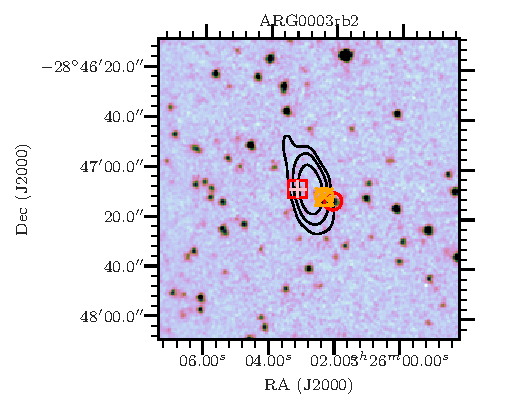
\includegraphics[width=\textwidth]{atlas-images/examples_all/example_sorted_2_0.pdf}
            \caption{\DIFaddFL{One resolved component and resolved source.}}
        \end{subfigure}
        \begin{subfigure}{0.45\textwidth}
            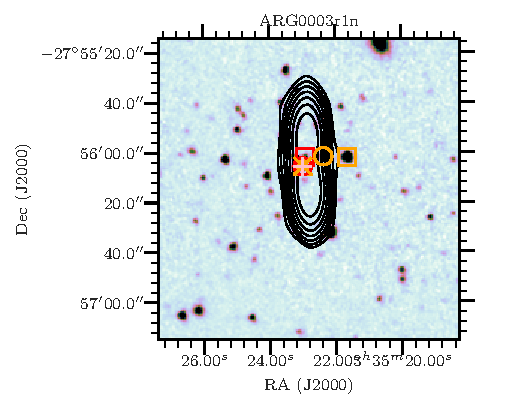
\includegraphics[width=\textwidth]{atlas-images/examples_all/example_sorted_3_454.pdf}
            \caption{\DIFaddFL{Three resolved components comprising one resolved source.}}
        \end{subfigure}
        \begin{subfigure}{0.45\textwidth}
            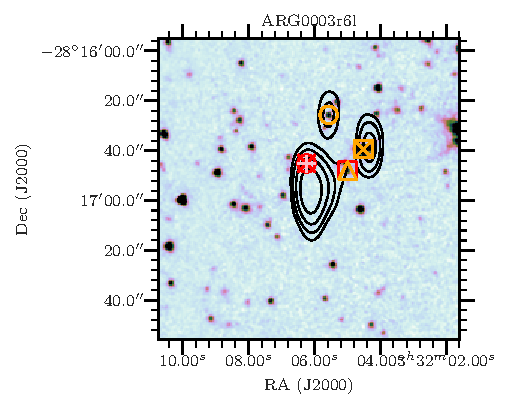
\includegraphics[width=\textwidth]{atlas-images/examples_all/example_sorted_4_264.pdf}
            \caption{\DIFaddFL{Three resolved components comprising one resolved source.}}
        \end{subfigure}
        \begin{subfigure}{0.45\textwidth}
            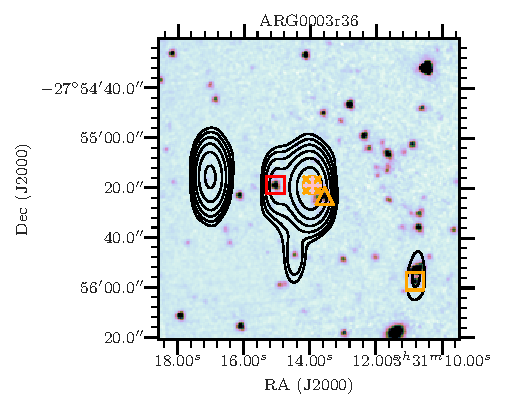
\includegraphics[width=\textwidth]{atlas-images/examples_all/example_sorted_5_207.pdf}
            \caption{\DIFaddFL{Three resolved components comprising one resolved source.}}
        \end{subfigure}
        \begin{subfigure}{0.9\textwidth}
            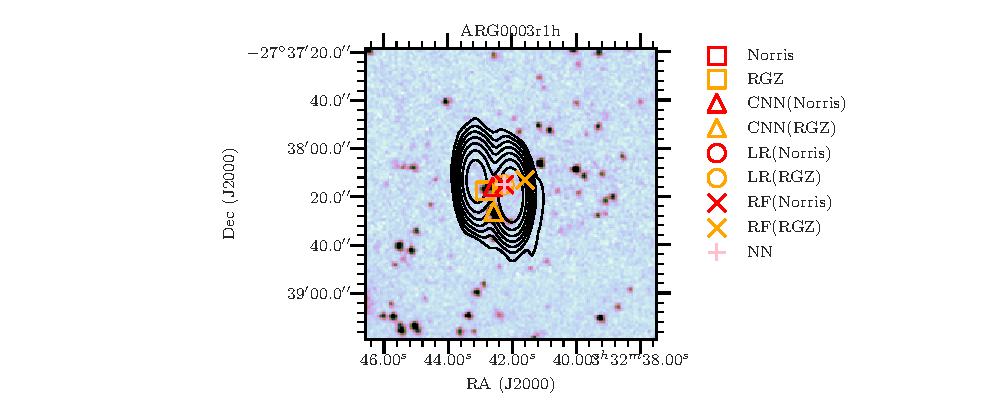
\includegraphics[width=\textwidth]{atlas-images/examples_all/example_sorted_0_306.pdf}
            \caption{\DIFaddFL{Two compact components, each a compact source.}}
        \end{subfigure}
        \caption[Examples of resolved sources with high disagreement between cross-identifiers.]{\label{fig:examples} \DIFaddFL{Examples of resolved sources with high disagreement between cross-identifiers. The contours show ATLAS radio data and start at $4\sigma$, increasing geometrically by a factor of 2. The background image is the }\unit{3.6}{\micro\meter} \DIFaddFL{SWIRE image. Binary classifier model/training set combinations are denoted $C(S)$ where $C$ is the binary classifier model and $S$ is the training set. `LR' is logistic regression, `CNN' is convolutional neural networks, and `RF' is random forests. `Norris' refers to the expert labels and `RGZ' refers to the Radio Galaxy Zoo labels. The cross-identification made by nearest neighbours is shown by `NN'.}}
    \end{figure}


\unappendix

\DIFaddend %!tex root=./thesis.tex
\chapter{Radio Luminosity Functions}
\label{cha:rlfs}

% make James' picture of binary xid before partitioning and colour it with a value-ramped viridis.

% \section{Making Catalogues with Binary Cross-identification}
% \label{sec:rlfs-revisiting-cross-id}


% \section{FIRST paper...}

This chapter is based on my paper \emph{Radio Galaxy Zoo: Radio Luminosity Functions of Extended Sources}, by M. J. Alger, O. I. Wong, C. S. Ong, N. M. McClure-Griffiths, H. Andernach, L. Rudnick, S. S. Shabala, A. F. Garon, J. K. Banfield, A. D. Kapi\'nska, R. P. Norris, and A. J. M. Thomson; to be submitted. Some minor changes have been made to match the rest of this thesis.\\

In \autoref{cha:cross-id}, we concluded that our machine learning cross-identification approach was sound in principle, but the small size and lack of morphological complexity in ATLAS prevented training a good classifier. To demonstrate this, we turned our attention to the Faint Images of the Radio Sky at Twenty Centimeters (FIRST) survey, which contained many more sources and many more morphologically complex sources due to its higher resolution and sample size. If cross-identification of this dataset was successful, we could use the resulting cross-identification catalogue to investigate statistical properties of radio galaxies at larger scales than previously possible. The object of interest would be the radio luminosity function (RLF), a statistical description of how common radio galaxies of various luminosities are throughout the \DIFdelbegin \DIFdel{universe}\DIFdelend \DIFaddbegin \DIFadd{Universe}\DIFaddend . The RLF would be specific to only extended radio galaxies, and it is this class of galaxies that we would expect to maximally impact its local environment through direct, mechanical energy input.

In this chapter, we use a machine learning model trained on the Radio Galaxy Zoo citizen science project to cross-identify \ncomponents{} radio components of extended radio sources from FIRST with \nsources{} host galaxies observed in the mid-infrared from the All\emph{WISE} source catalogue. \nsourceszsp{} hosts have a spectroscopic redshift in the Sloan Digital Sky Survey (SDSS). This is the largest available sample of cross-identified extended radio sources to date at the time of writing. The large sample size allows us to estimate the RLF of extended radio galaxies and to further characterise the sample with fractional radio luminosity functions. The extended source RLF can be used to estimate the mechanical energy injected into the local \DIFdelbegin \DIFdel{environment }\DIFdelend \DIFaddbegin \DIFadd{environments }\DIFaddend of active galactic nuclei (AGN). We estimate from the observed radio emission that inferred extended radio jets from AGN contribute between $1.3 \times 10^{30}$ and $1.2 \times 10^{32}$~W~Mpc$^{-3}$ of mechanical energy to their environment throughout the low-redshift ($z < 0.6$) Universe. By further visual verification we also find \nnewgiants{} radio galaxies with projected size larger than 1~Mpc. Our results directly demonstrate the impact that automated machine learning methods could have on future wide-area radio surveys.

\section{Introduction} \label{sec:rlfs-intro}

Radio active galactic nuclei (AGN) are some of the most violent and energetic
objects in the Universe. Supermassive black holes at the \DIFdelbegin \DIFdel{centre }\DIFdelend \DIFaddbegin \DIFadd{centres }\DIFaddend of galaxies
can produce large, luminous radio jets that may feed lobes extending up to
megaparsec scales. As a vital part of galaxy evolution, we want to understand
how radio AGN interact with their host galaxies, in what kinds of galaxies
these AGN are found, and how these populations change over cosmic time.

Mechanical energy from AGN is needed to explain the star-formation history of galaxies throughout the Universe \citep[e.g.][]{raouf17agn,hardcastle20feedback}. The radio luminosity function (RLF) of extended radio sources \DIFdelbegin \DIFdel{would characterise }\DIFdelend \DIFaddbegin \DIFadd{characterises }\DIFaddend the energy output of galaxies capable of significant energy impact into their local environment. The local RLF of primarily compact sources is estimated and
described in detail by \citet{mauch07rlf}, \citet{pracy16rlf} and
\citet{condon19rlf}, each with complete volume-limited samples. However, the RLF of extended radio sources has not been
characterised as a separate sample, because estimating this RLF would need a large number of extended sources with known
redshifts. Such redshifts are usually obtained by cross-matching the radio
sources with their host galaxies in the optical or infrared. While this
cross-matching is relatively straightforward for compact/unresolved sources,
and can therefore be automated \citep[e.g.][]{kimball08}, extended radio
emission may be complex and may not be co-located with the host galaxy.
Cross-identification of complex, extended sources is therefore usually done
manually, limiting the sample size.

Wide-area radio surveys like the Very Large Array Faint Images of the Sky at
Twenty Centimeters survey \citep[FIRST;][]{white97first} have led to
catalogues of hundreds of thousands of radio objects, most of which are
associated with radio AGN \citep{sadler02rlf}. While individual galaxy
properties vary significantly between galaxies, the large sample size of
such surveys allows us to examine reliable bulk statistics that may
tightly constrain models and \DIFdelbegin \DIFdel{theory }\DIFdelend \DIFaddbegin \DIFadd{theories }\DIFaddend of radio galaxy evolution and formation \citep{condon92radio}. With a
sufficiently large sample \citep[of size $N$ such that $N \gg
\sqrt{N}$;][]{condon91rlf} we can also divide the RLF into fractions based
on the physical properties of each galaxy. These \defn{fractional RLFs} show
how different physical processes comprise the luminosity distribution, and
can be used to investigate how these processes relate to the properties of
the AGN.

In this chapter we calculate the RLF for extended radio sources in FIRST. Throughout this chapter we define an \defn{extended radio source} as a collection of extended radio components with the same host galaxy, and following
\citet{banfield15} we define an \defn{extended radio component} as a radio
component which fulfils \autoref{eq:rgz-criterion}:
\begin{equation}
    \frac{S_{\mathrm{peak}}}{S_{\mathrm{int}}} < 1 - \frac{0.1}{\log_{10}(S_{\mathrm{peak}} / 1\ \mathrm{mJy})},
    \label{eq:rgz-criterion}
\end{equation}
where $S_{\mathrm{peak}}$ is the peak radio flux density and
$S_{\mathrm{int}}$ is the integrated radio flux density. We define \defn{radio components} as Gaussians fit to
radio emission, \defn{radio islands} as connected patches of radio emission
above a local $4\sigma$ value, and \defn{radio sources} as sets of radio
islands or components associated with the same galaxy. The radio flux density of a source is the sum of the flux densities of the components according to the FIRST catalogue. The \defn{(infrared)
host galaxy} of a radio source or component is defined as the infrared galaxy
associated with the radio emitter. A \defn{cross-identification} is an
association of a host galaxy with one or more radio components or islands. We
define \defn{candidate host galaxies} (or simply
\defn{candidates}) as infrared objects that are near a radio component on
the sky and thus may potentially be the host galaxy of that component.

Upcoming
radio surveys such as the Evolutionary Map of the Universe
\citep[EMU;][]{norris11} are expected to increase the number
of complex radio sources to around 7 million \citep{banfield15}. Manual, expert cross-identification for such surveys will be impractical. One way forward could be to ask non-expert volunteers for help with manual cross-identification, which \DIFdelbegin \DIFdel{is }\DIFdelend \DIFaddbegin \DIFadd{was }\DIFaddend the approach taken by Radio Galaxy Zoo \citep[RGZ;][]{banfield15}. This is called \defn{citizen science} and has been employed successfully in many fields with large datasets \citep{marshall15citizen}. Even this approach is not sufficient for 7 million sources, though, with RGZ cross-identifying around 75~000 sources in four years. Machine
learning provides a potential pathway to obtaining useful physics from such
large samples.

In this chapter, we train a machine learning model based on \citet{alger18radio}, using RGZ as training data, and
use this model to automatically cross-identify \ncomponents{} radio components catalogued by FIRST. This results in \nsourceszsp{} sources
with spectroscopic redshifts. This is the largest available catalogue of
extended radio source cross-identifications. We call our catalogue
\defn{RGZ-extrapolated} or \defn{RGZ-Ex}. Due to our large sample size we are able to further divide the
source population by properties of the host galaxies. We refer to the trained machine learning model and the associated cross-identification algorithm jointly as \defn{binary cross-identification}, or \defn{BXID}. Note that there are two stages to our automated approach: \DIFdelbegin \DIFdel{first}\DIFdelend \DIFaddbegin \DIFadd{First}\DIFaddend , we train BXID using an existing catalogue of cross-identified sources; second, we generate new cross-identifications for radio components not in the training catalogue. We refer to these stages as \defn{training} and \defn{prediction} respectively. Our data sources are described in \autoref{sec:rlfs-data}. Our approach is discussed in \autoref{sec:rlfs-method}. Radio luminosity functions of extended sources are presented in \autoref{sec:rlfs-rlf} and we discuss these functions in \autoref{sec:rlfs-discussion}.

Throughout this chapter we assume a flat $\Lambda$-CDM cosmology of \linebreak $H_0 =
69.3$~km~s$^{-1}$~Mpc$^{-1}$, $\Omega_m = 0.287$. These are the cosmological
parameters from the Nine-year Wilkinson Microwave Anisotropy Probe
\citep[WMAP9;][]{hinshaw13wmap9}.

\section{Data} \label{sec:rlfs-data}

In this section we describe how we obtain our training and prediction data. To enable the estimation of the extended RLF, we apply a number of selection criteria to the data which are shown in \autoref{fig:sankey-sources}.

    \subsection{RGZ} \label{sec:rlfs-rgz-data}

    RGZ is a citizen science project that aims to cross-identify complex radio sources with mid-infrared host galaxies with the help of volunteers. The first RGZ data release contains around 75~000 cross-identifications of a random subset of extended sources in FIRST with their host galaxies in All\emph{WISE}. For more details on RGZ see \citet{banfield15}. This catalogue has also been used in other machine learning contexts, including supervised learning for source aggregation \citep{wu19claran} and unsupervised learning methods \citep{galvin19som,ralph19ae}. We discard the RGZ sources without a host galaxy detected in All\emph{WISE} and use the remaining 41~446 sources for training.

    The RGZ catalogue only contains sources with at least 0.65 weighted volunteer agreement, equivalent to approximately 80 per cent reliability. This implicitly selects for less complex sources, since the volunteer agreement is a proxy for the difficulty of cross-identifying a source (Wong et al. in prep\DIFaddbegin \DIFadd{.}\DIFaddend ).

    \subsection{FIRST} \label{sec:rlfs-first-data}

    We use radio imagery and select radio components from the FIRST survey and associated catalogue respectively \citep{white97first,helfand15first}. FIRST is a
    1.4~GHz radio survey covering 10~575~deg$^2$ of the sky north of $\mathrm{Dec} = -10^\circ$ with an angular resolution of $5.4''$. At a detection limit of $1$~mJy, the catalogue contains 946~432 radio components.

    For both training and prediction, we make use of image cutouts from FIRST centred on mid-infrared candidate hosts. We predict host galaxies for the \ncomponents{} extended FIRST components detected at $>10\sigma$ \citep[about 1.5~mJy~beam$^{-1}$, per][]{banfield15} that have complete radio imagery for all candidate hosts. \DIFaddbegin \DIFadd{The numbers of objects removed by our quality filters are shown in }\aref{sec:rlfs-sankey}\DIFadd{.
}\DIFaddend 

    \subsection{All\emph{WISE}} \label{sec:rlfs-wise-data}

    We use the sky coordinates and magnitudes from the All\emph{WISE} \citep{cutri2013wiseexplanatory} catalogue during training and prediction. All\emph{WISE} is an all-sky catalogue of mid-infrared objects detected by the \emph{Wide-field Infrared Survey Explorer} \citep[\emph{WISE}][]{wright10wise} at 3.4, 4.6, 12\DIFaddbegin \DIFadd{, }\DIFaddend and \unit{22}{\micro\meter} wavelengths (called $W1$--$W4$, respectively). All\emph{WISE}
    contains over 747~million objects detected above $5\sigma$ at 3.4 and
    \unit{4.6}{\micro\meter}. \emph{WISE} has an angular resolution of
    $6.1''$ and $6.4''$ at these wavelengths, respectively.

    We store All\emph{WISE} objects in a
    \texttt{MongoDB}\footnote{\url{https://www.mongodb.com/}} database with
    a geospatial index on the right ascension and declination. This allows
    us to perform fast spatial lookups. The geospatial index in
    \texttt{MongoDB} assumes a perfectly spherical Earth with a fixed radius, allowing us to use it for sky coordinate
    searches. We use the right ascension and declination of All\emph{WISE} sources to generate candidate hosts by searching for infrared sources near FIRST components.

    \subsection{SDSS} \label{sec:rlfs-sdss-data}

    While we do not use data from the Sloan Digital Sky Survey Data Release 15 \citep[SDSS;][]{sdss} for training or prediction, we do use SDSS for spectroscopic redshifts of our host galaxies. These redshifts are required to calculate the radio \DIFdelbegin \DIFdel{luminosity }\DIFdelend \DIFaddbegin \DIFadd{luminosities }\DIFaddend of our sources. We use CDS X-Match\footnote{\url{http://cdsxmatch.u-strasbg.fr/}} to match each infrared host galaxy to the closest source imaged by SDSS to within $5''$. This results in \nsourceszsp{} spectroscopic redshifts for our \nsources{} total host galaxies. To estimate the rate of false association with SDSS sources, we add a $1'$ offset to all host positions and redo the matching process. With this method we estimate a $0.4$ per cent rate of false association.

\section{Method}\label{sec:rlfs-method}

We apply the binary classification cross-identification method (BXID) following \citet{alger18radio}. This method casts cross-identification
as a classification problem where infrared `candidate host galaxies' are
classified as either being host galaxies or not. A classifier is trained
on examples of host galaxies and non-host galaxies drawn from a
cross-identification catalogue, for which we use RGZ. Other related
algorithms developed to automatically cross-identify radio objects
include Bayesian methods \citep{fan15}, likelihood ratio \citep{weston18lrpy},
 positional matching \citep[e.g.][]{kimball08, norris06, middelberg08}, and positional/image hybrid approaches \citep{van_velzen_radio_2012}, but these methods do not make use of existing
cross-identification catalogues and most assume compact radio sources or that the projected radio emission overlaps the host galaxy.

\begin{table}
  \caption{Medians and standard deviations used to normalise input features \DIFaddbeginFL \DIFaddFL{for our classifiers}\DIFaddendFL .
    \label{tab:medians-stdevs}}
    \centering
  \begin{tabular}{ccc}
    \hline\hline
    Feature & Median & Standard deviation\\
    \hline
    Radio image & \unit{13.2}{\micro{}Jy} & \unit{3.01}{\milli{}Jy}\\
    $W1 - W2$ & 0.289 mag & 0.378 mag\\
    $W1 - W3$ & 4.350 mag & 1.067 mag\\
    $W1 - W4$ & 7.853 mag & 1.144 mag\\
    $W2 - W3$ & 4.016 mag & 0.958 mag\\
    $W2 - W4$ & 7.541 mag & 1.046 mag\\
    $W3 - W4$ & 3.518 mag & 0.409 mag\\
    $W1$ & 16.659 mag & 1.154 mag\\
    \hline\hline
  \end{tabular}
\end{table}

We represent candidate host galaxies by a $2' \times 2'$ radio image from FIRST centred on that galaxy, the \unit{3.4}{\micro\meter} magnitude, and the six colours (magnitude differences) derived from the four \emph{WISE} wavelengths. Unknown values of infrared flux were set to their upper limits in All\emph{WISE}. We note
that many $W3-W4$ colours are missing, so this feature may be less useful than
the others. We normalise the colours and \DIFdelbegin \DIFdel{magnitude }\DIFdelend \DIFaddbegin \DIFadd{magnitudes }\DIFaddend by subtracting the median and
dividing by the standard deviation. We normalise each
pixel in each radio image by subtracting the median, dividing by the standard
deviation, and applying a logistic function ($\sigma$;
\autoref{eq:logistic}) to account for the high dynamic range of radio
images.
\begin{equation}
  \sigma(a) = \frac{1}{1 + \exp(-a)}
  \label{eq:logistic}
\end{equation}
The medians and standard deviations are reported in \autoref{tab:medians-stdevs}. These values are computed across the training set.

For each FIRST component we generate a set of candidate host galaxies.
An All\emph{WISE} object is considered a candidate host for a radio
component if it is within $\sqrt{2} \times 1.5'$ of the centre of the two-dimensional
Gaussian fit for that component. This search radius is the maximum
angular distance that a host galaxy can be located in RGZ due to the
$3'$-wide square images shown to volunteers. Candidate hosts are
assigned binary labels: All candidates identified as host galaxies in
RGZ are assigned a positive label and all others are assigned a
negative label. Following \citet{alger18radio} we train a convolutional neural
network (CNN) on the labelled candidate hosts. We
base our model on \texttt{ResNet18} \citep{he2016resnet} pretrained on the
ImageNet classification task, with the final layer removed and replaced
by a logistic regression model. Non-image features (i.e. colours and the
\unit{3.6}{\micro\meter} magnitude) are concatenated with the features
that are output by the final \texttt{ResNet18} layer. Using \texttt{Adam}
\citep{kingma14adam} to optimise our weights, we train this model on our
task until binary cross-entropy loss starts to increase on a
randomly-selected 20 per cent validation set. We use \texttt{PyTorch}
\citep{paszke2017pytorch} to implement this model. The scores of each FIRST
component are weighted by a one-dimensional Gaussian function of angular separation, and the
candidate maximising this weighted score is selected as the host galaxy. We
set the standard deviation of the Gaussian to $120''$ as this provides good
empirical results.

92 per cent of the host galaxies in RGZ \DIFdelbegin \DIFdel{are }\DIFdelend \DIFaddbegin \DIFadd{were }\DIFaddend also detected as host galaxies in RGZ-Ex. The mean volunteer agreement on all RGZ sources with detected hosts was $95^{+5}_{-13}$ per cent, compared to $88^{+12}_{-17}$ per cent for sources with hosts not in RGZ-Ex. Incorrect cross-identifications can be considered a source of noise in the statistics. In future work we will design a way for BXID to output an `uncertainty' so \DIFaddbegin \DIFadd{that }\DIFaddend sources with uncertain cross-identifications can be removed from calculations. We quantify the reliability of RGZ-Ex in \autoref{sec:rlfs-manual-validation}.

We note that BXID necessarily identifies a host galaxy for all radio emission, even when it does not
make sense to do so. In our current work we treat this as a source of
noise. Future extensions to BXID will allow it to output `no detected
host'.

    \subsection{Visual verification}\label{sec:rlfs-manual-validation}

    To quantify the reliability of RGZ-Ex, \DIFdelbegin \DIFdel{some of the authors }\DIFdelend \DIFaddbegin \DIFadd{we }\DIFaddend (M.A., O.W., A.K., N.M., and A.T.) visually verified a randomly selected set of 200 radio components/host galaxy pairs in RGZ-Ex. For each pair we decided whether the radio component matched its identified host or not. This allowed us to estimate the accuracy of radio component-infrared host pairs identified by BXID. Verification of component-host pairs is noisy and sometimes even subjective, so each author looked at all 200 components. If an author was unsure about a pair, they were allowed to ignore it and the verification was treated as missing label data. We then aggregated these verifications following the aggregation approach introduced by \citet{dawid79em}. This approach jointly estimates the accuracy of each author along with the aggregated verification by maximising the joint likelihood. Note that this approach is able to handle missing label data. We propagated the uncertainty in the accuracy with a Monte Carlo approach, sampling aggregated verifications from the probabilities resulting from the \citeauthor{dawid79em} model. The estimated accuracy of BXID \DIFdelbegin \DIFdel{is }\DIFdelend \DIFaddbegin \DIFadd{was }\DIFaddend $(89.5 \pm 0.8)$ per cent. It is interesting to note from our results that even astronomers disagree significantly on the radio cross-identification task, with agreement between authors ranging from 50 to 100 per cent across the verification components. We report the full verification set in \DIFdelbegin %DIFDELCMD < \autoref{sec:rlfs-verification-appendix}%%%
\DIFdelend \DIFaddbegin \aref{sec:rlfs-verification-appendix}\DIFaddend .

\section{Radio luminosity functions}
\label{sec:rlfs-rlf}

  \begin{figure}
      \centering
    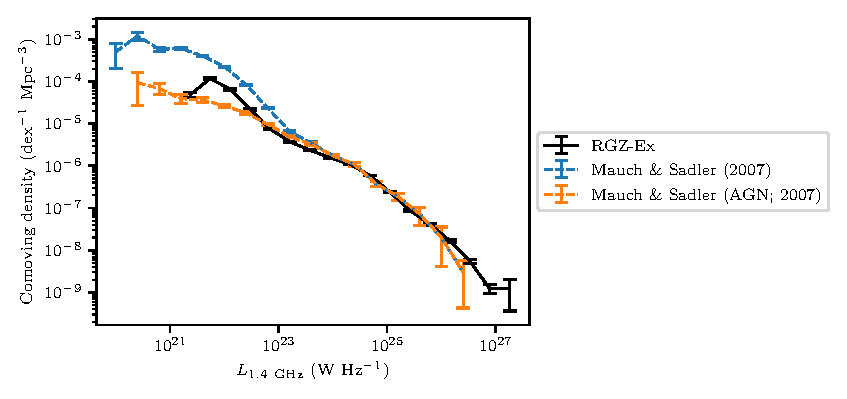
\includegraphics{rlf-images/rlf.pdf}
    \caption{RGZ-Ex radio luminosity function compared with the RLFs of \citet{mauch07rlf}.
      \label{fig:rlf}}
  \end{figure}

  In this section we present our radio luminosity functions (RLFs) derived
  from the RGZ-Ex catalogue. \DIFaddbegin \DIFadd{We first eliminated sources and components with high sidelobe probability according to the FIRST catalogue and low BXID scores (see }\aref{sec:rlfs-sankey} \DIFadd{for a diagram of this filtering process). }\DIFaddend To calculate each RLF we 
  followed the $1/V_{\max}$ method \citep{schmidt1968vmax}. This method accounts for the effects of Malmquist bias, which is a systematic bias against sources at greater distances. We
  describe this approach in \DIFdelbegin %DIFDELCMD < \autoref{sec:rlfs-rlf-desc}%%%
\DIFdel{. We limit }\DIFdelend \DIFaddbegin \aref{sec:rlfs-rlf-desc}\DIFadd{. We limited }\DIFaddend our sample to radio sources with
  \unit{1.4}{\giga\hertz} integrated flux density of at least \unit{2}{\milli Jy}
  associated with host galaxies brighter than magnitude 17 at
  \unit{3.4}{\micro\meter}, a spectroscopic redshift $0.02 \leq z \leq 0.6$,
  and an $i$-band magnitude $<20$. We chose these
  limits based on the distribution of redshifts and infrared magnitudes as well as the sensitivity of FIRST. We then \DIFdelbegin \DIFdel{remove }\DIFdelend \DIFaddbegin \DIFadd{removed }\DIFaddend sources with unusually high or low \DIFdelbegin \DIFdel{W1 }\DIFdelend \DIFaddbegin \DIFadd{$W1$ }\DIFaddend magnitude for their redshift (more than \DIFdelbegin \DIFdel{3 }\DIFdelend \DIFaddbegin \DIFadd{three }\DIFaddend standard deviations from the mean) because many such sources \DIFdelbegin \DIFdel{have }\DIFdelend \DIFaddbegin \DIFadd{had }\DIFaddend incorrect spectroscopic redshifts, e.g. blazars. There \DIFdelbegin \DIFdel{are }\DIFdelend \DIFaddbegin \DIFadd{were }\DIFaddend \nsourcesrlf{} sources matching all criteria. We \DIFdelbegin \DIFdel{assume }\DIFdelend \DIFaddbegin \DIFadd{assumed }\DIFaddend a spectral index of $\alpha = -0.7$ \citep[as is common in literature, e.g.][]{condon02radio} with flux density $f \propto \nu^{\alpha}$ where $\nu$ is the frequency. We \DIFdelbegin \DIFdel{calculate }\DIFdelend \DIFaddbegin \DIFadd{calculated }\DIFaddend the $k$-corrected radio luminosity \citep{kochanek01kband} as follows:
  \begin{equation}
      \label{eq:luminosity}
      L = \frac{4\pi f d^2}{1+z}{(1+z)^{-\alpha}}
  \end{equation}
  where $z$ is redshift and $d$ is luminosity distance (a function of $z$).
  Uncertainties in comoving density \DIFdelbegin \DIFdel{are }\DIFdelend \DIFaddbegin \DIFadd{were }\DIFaddend estimated as described in \DIFdelbegin %DIFDELCMD < \autoref{sec:rlfs-rlf-desc}%%%
\DIFdelend \DIFaddbegin \aref{sec:rlfs-rlf-desc}\DIFaddend . Completeness estimates are shown in \DIFdelbegin %DIFDELCMD < \autoref{sec:rlfs-completeness}%%%
\DIFdelend \DIFaddbegin \aref{sec:rlfs-completeness}\DIFaddend . We discuss biases in our methods and results in \autoref{sec:rlfs-bias}.

  We \DIFdelbegin \DIFdel{compare }\DIFdelend \DIFaddbegin \DIFadd{compared }\DIFaddend our RLFs with \citet{mauch07rlf}, who estimated RLFs from 7~824
  manually cross-identified radio sources in the NRAO VLA Sky Survey \citep[NVSS;][]{condon98nvss}.
  Their RLFs were split into AGN and star-forming radio sources. While we
  \DIFdelbegin \DIFdel{do }\DIFdelend \DIFaddbegin \DIFadd{did }\DIFaddend not make this split explicitly in our catalogue, we \DIFdelbegin \DIFdel{expect }\DIFdelend \DIFaddbegin \DIFadd{expected }\DIFaddend both RGZ-Ex
  and RGZ to be dominated by AGN due to the selection criterion of being extended in the selected redshift volume. We note that the redshift range used in our work, $0.02 < z < 0.6$, differs from the $0.003 < z < 0.3$ range used by \citet{mauch07rlf}.

  In \autoref{fig:rlf} we show the RLF derived from RGZ-Ex along with the RLFs from \citet{mauch07rlf}. There is good
  agreement between all three luminosity functions for luminosities greater than $10^{23}$~W~Hz$^{-1}$
  and below this luminosity the RGZ-Ex RLF is bounded above by the
  \citet{mauch07rlf} RLF. RGZ-Ex generally finds less comoving density than \citet{mauch07rlf}, which we attribute to our requirement for extent. We suggest that the peak in RGZ-Ex RLF at approximately $10^{22}$~W~Hz$^{-1}$ is due to our sample containing a small fraction of star-forming galaxies. Our criterion, however, \DIFdelbegin \DIFdel{does cut }\DIFdelend \DIFaddbegin \DIFadd{cuts }\DIFaddend out most star-forming regions as these are often compact, which is why we report lower densities than the star-forming RLF of \citet{mauch07rlf}.

\begin{figure}
    \centering
    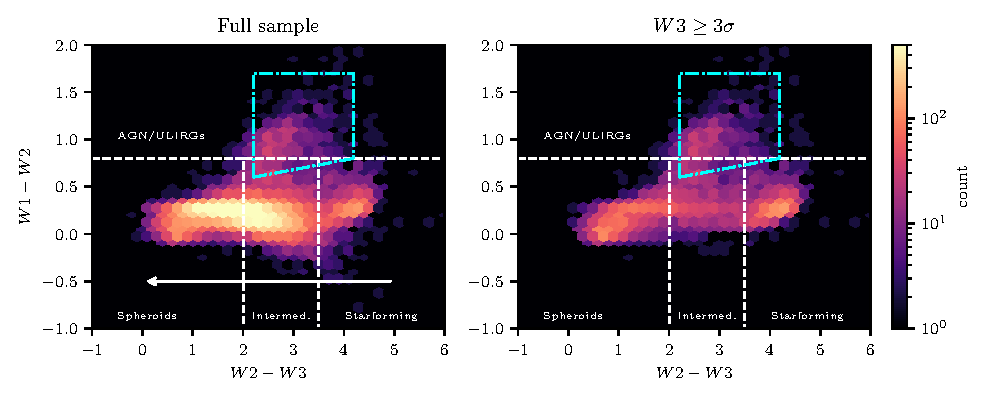
\includegraphics[width=\linewidth]{rlf-images/colour-colour.pdf}
    \caption[\emph{WISE} colour-colour distributions.]{\emph{WISE} colour-colour distributions. The dashed grey lines show
      simple host galaxy class divisions from \citet{jarrett17wise}. These
      classes are labelled in the plot. The blue dot-dashed line shows
      the empirical optical/infrared AGN criteria from \citet{jarrett11wise}. The arrow shows the direction that galaxies would shift with fainter $W3$ magnitudes. The right plot limits the sample to only sources with $W3 \geq 3 \sigma$.
      \label{fig:colour-colour}}
  \end{figure}

  \begin{figure}
      \centering
    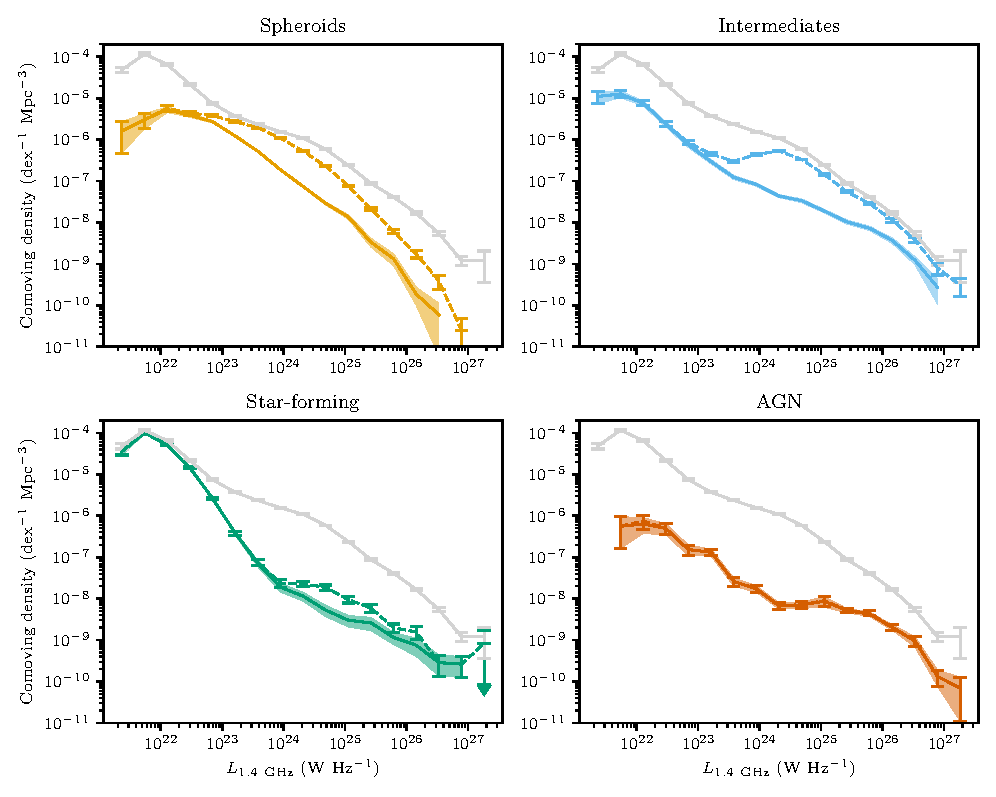
\includegraphics[width=\linewidth]{rlf-images/frlf-ir-colours.pdf}
    \caption[RLFs split by \emph{WISE} colour regions.]{RLFs split by host galaxy
      location in the \emph{WISE} colour-colour plot (\autoref{fig:colour-colour}),
      using our automated cross-identifications. The grey line is the
      total RLF for all sources. Solid lines have good $W3$ detections and dashed lines include $W3$ with low signal-to-noise.
    \label{fig:fractional-rlf}}
  \end{figure}

      The \emph{WISE} colour-colour plot, shown for RGZ-Ex in
      \autoref{fig:colour-colour}, is often used to categorise galaxies at different evolutionary stages into
      four mid-infrared colour regions that are typically populated by 1)
      spheroidals or elliptical galaxies; 2) quasi-stellar objects (QSOs),
      Seyferts or powerful AGN; 3) starbursting or luminous infrared galaxies
      (LIRGs); and 4) the intermediate region where the other three regions
      overlap. The horizontal axis, $W2-W3$, separates early- and late-type galaxies, with the star-forming late-type galaxies appearing redder (further to the right) \citep{wright10wise}. The vertical axis, $W1-W2$, separates inactive galaxies from AGN
      with strongly radiating accretion discs \citep{sadler14radio}. In
      \autoref{fig:fractional-rlf} we show the radio luminosity function split
      by host galaxy location in the mid-infrared colour-colour plot as defined by \citet{jarrett17wise}.

      Many sources have $W3$ detections with low signal-to-noise, limiting our ability to subdivide our sample. We plot both the RLFs for the sample with only $W3 \geq 3 \sigma$ as well as the RLFs for the full sample in \autoref{fig:fractional-rlf}. For the full sample we use the lower magnitude limit from All\emph{WISE} as the $W3$ magnitude (which is an upper flux limit). Using the upper flux limit as the real $W3$ flux has the effect of increasing $W2 - W3$ compared to a real detection, so objects appear further to the right of the colour-colour diagram (\autoref{fig:colour-colour}) than they ought to. This means that due to $W3$ limits, objects that should be in the spheroid set \DIFdelbegin \DIFdel{will }\DIFdelend \DIFaddbegin \DIFadd{instead }\DIFaddend appear in the intermediate and star-forming sets, and objects from the intermediate set \DIFdelbegin \DIFdel{will }\DIFdelend \DIFaddbegin \DIFadd{instead }\DIFaddend appear in the star-forming set.

      At low luminosities, our extended source RLF is dominated by galaxies with infrared
      colours consistent with star formation. The fraction
      of the RLF composed of the star-forming set drops off rapidly for
      $L_{1.4\ \mathrm{GHz}} > 10^{22}$~W~Hz$^{-1}$, as expected for galaxies with radio emission
      dominated by star formation \citep[e.g.][]{mauch07rlf}. However, the RLF slope flattens out again beyond $10^{24}$~W~Hz$^{-1}$, suggesting a second source population. This population has many missing $W3$ measurements, and these are likely intermediates or spheroids incorrectly included in the star-forming set. We therefore suggest that the
      low-luminosity RGZ-Ex sample mostly contains nearby galaxies with radio
      emission due to star formation, which appear extended in FIRST as they
      are close enough for FIRST to resolve their
      disc (greater than 20~kpc at $z = 0.2$). The remaining fraction of star-forming sources found by
      \citet{mauch07rlf}, shown in
      \autoref{fig:rlf}, would not be resolved in FIRST, as they are small or
      distant.

      Spheroids, which are hosts in the mid-infrared region corresponding to ellipticals and stars \citep{wright10wise}, comprise the majority of radio galaxies at $10^{23}$~W~Hz$^{-1}$,
      and have a peak density at $10^{22}$~W~Hz$^{-1}$. The common host galaxies for radio-loud AGN tend to be passively-evolving spheroids. It is not surprising that they are more common than star-forming galaxies at luminosities greater than $10^{22}$~W~Hz$^{-1}$. Above
      $10^{25}$~W~Hz$^{-1}$ they are less common than intermediate galaxies and
      their contribution to the luminosity function drops rapidly. This is likely due to the loss of $W3$ detections moving spheroids into the intermediate set, and we hypothesise that with deeper $W3$ observations spheroids may dominate above $10^{25}$~W~Hz$^{-1}$.

      Sources with hosts in the mid-infrared AGN region of the colour-colour diagram (\autoref{fig:colour-colour}) make
      up the smallest contribution to the radio luminosity function. They have
      a steadily decreasing density from their lowest observed $L_{1.4\ \mathrm{GHz}}$ of $10^{22}$~W~Hz$^{-1}$ to their highest of
      $10^{27}$~W~Hz$^{-1}$, but are present in all luminosity bins except for
      the very lowest. This is a set with a very low fraction of spectroscopic SDSS matches for the \emph{WISE} host galaxies. 26 per cent of
      hosts outside the \emph{WISE} AGN region have an SDSS match, compared to just 12 per
      cent of hosts inside the \emph{WISE} AGN region. This is likely due to the incomplete sampling of QSOs in the SDSS spectroscopic survey or redshift evolution effects \citep{strauss02sdss}. The fraction of the RLF contributed by galaxies classed as mid-infrared AGN increases above $10^{25}$~W~Hz$^{-1}$, meaning that high-luminosity radio AGN are also more likely to be infrared AGN than at lower radio luminosities. Note that the AGN set is unaffected by missing $W3$ detections, as the AGN set is based only on $W1-W2$.

      Galaxies residing in the intermediate mid-infrared colour region can be
      populated by both early- and late-type galaxies, which have a mix of
      processes \DIFdelbegin \DIFdel{occuring }\DIFdelend \DIFaddbegin \DIFadd{occurring }\DIFaddend within them. These `intermediate sources' dominate in
      most luminosity ranges, and above $10^{24}$~W~Hz$^{-1}$ they comprise the
      vast majority of our sample. As intermediate-type galaxies fall between
      star-forming galaxies and passive ellipticals on the mid-infrared colour-colour plane, they do
      not have a clear morphological class and are composed of overlapping subsets of sources. The most luminous radio AGN are almost entirely found in
      this set of galaxies. In fact, as radio luminosity increases\DIFaddbegin \DIFadd{, }\DIFaddend the density
      fraction shifts from spheroids toward intermediate galaxies, likely due to missing $W3$ moving objects from the spheroid set into the intermediate set.

      \begin{figure}
          \centering
        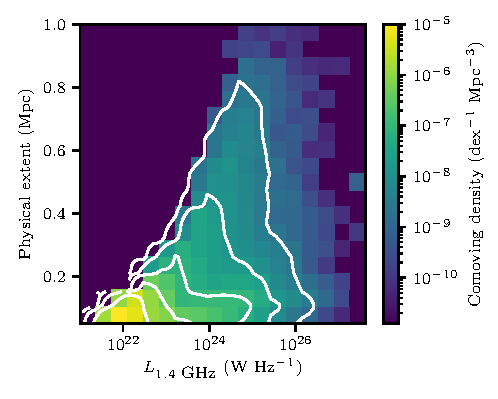
\includegraphics{rlf-images/physical-extent.pdf}
        \caption[Bivariate radio luminosity function showing radio luminosity against projected physical extent.]{Bivariate radio luminosity function showing radio luminosity against projected physical extent. Contours are on a log scale, starting at the median and increasing by 10 per cent per contour.
        \label{fig:fractional-rlf-extent}}
      \end{figure}

      In \autoref{fig:fractional-rlf-extent} we show the radio luminosity
      function for different ranges of projected physical extent of their radio emission. We estimate the angular extent as the angular distance between the most separated components in a multi-component source. This result is complementary to other Radio Galaxy Zoo studies on the effect of the environment on the size and asymmetry of the observed extended radio emission \citep{rodman19asymmetry,garon19bending}.


\section{Discussion}\label{sec:rlfs-discussion}

  \subsection{Biases and uncertainties}
    \label{sec:rlfs-bias}

    Biases enter our work due to our chosen samples and methods. Our training set,
    RGZ, is biased toward sources smaller than $1.5'$ and limited above by $\sqrt{2}
    \times 3'$ due to the $3' \times 3'$ cutout size of the RGZ user
    interface. RGZ volunteers preferentially select host
    galaxies that are brighter in $W1$, so we expect RGZ to overrepresent
    the number of sources with $W1$-bright host galaxies.

    These biases may affect our
    trained algorithm: \DIFdelbegin \DIFdel{for }\DIFdelend \DIFaddbegin \DIFadd{For }\DIFaddend example, the overabundance of $W1$-bright host
    galaxies in RGZ may cause our algorithm to be less accurate when
    unassociated bright galaxies are in the field of view. Without knowing the true
    distribution of host galaxies, however, it is difficult to quantify the
    effect of such biases on our trained method.

    FIRST itself is also biased. \citet{helfand15first} describe several reasons why FIRST flux may be systematically underestimated. Most of these effects are insignificant for extended objects in our sample or are corrected in the FIRST catalogue from which we draw our flux information. The exception is the `resolving out' of diffuse and low surface brightness radio emission by the Very Large Array in its B configuration. This means that we lose flux on most nearby radio galaxies (especially those with very
    diffuse components) and may miss diffuse or dim radio galaxies entirely.
    More diffuse radio galaxies such as Fanaroff-Riley type I \citep[FRI;][]{fanaroff1974} galaxies tend to
    be toward the low end of the radio-loud luminosity distribution, about
    $10^{23}$~W~Hz$^{-1}$ \citep{best09radio}, so we expect that losing
    diffuse sources would lower our estimates of density around this
    luminosity. Large, extended lobes such as those associated with Fanaroff-Riley type II \citep[FRII;][]{fanaroff1974} galaxies may also be resolved out, so by the same mechanism we expect to lose an increasing amount of flux with increasing source angular size. This effect is compounded by flux loss at 1.4~GHz associated with synchrotron losses and adiabatic expansion losses \citep{blundell99doubles}.

    Our host galaxy redshifts may be biased. Incorrectly identifying the host galaxy may introduce sources with incorrect redshifts into the RLF, an effect which will be dominated by misidentifying galaxies as hosts where the true host is not detected. Since we are matching to optical spectra in SDSS to find
    redshifts, we are biased toward brighter host galaxies \DIFdelbegin \DIFdel{that }\DIFdelend \DIFaddbegin \DIFadd{which }\DIFaddend are more
    likely to have such spectra. Without an optically-complete \DIFdelbegin \DIFdel{sample ---
    currently }\DIFdelend \DIFaddbegin \DIFadd{sample---currently }\DIFaddend impossible on such scales---this effect is unavoidable.
    Brighter optical sources appear at lower redshifts, so we likely
    undersample higher-redshift (and hence higher-luminosity) galaxies.

    Our requirement for radio emission to be extended \DIFdelbegin \DIFdel{will miss }\DIFdelend \DIFaddbegin \DIFadd{misses }\DIFaddend radio galaxies that would be resolved and extended if they were not aligned with the \DIFdelbegin \DIFdel{line of sight}\DIFdelend \DIFaddbegin \DIFadd{line-of-sight}\DIFaddend . We therefore must be underestimating the population of extended sources (though assuming a random distribution of orientations, the majority of galaxies \DIFdelbegin \DIFdel{will not be }\DIFdelend \DIFaddbegin \DIFadd{are not }\DIFaddend aligned close to the \DIFdelbegin \DIFdel{line of sight}\DIFdelend \DIFaddbegin \DIFadd{line-of-sight}\DIFaddend ). The requirement for extended radio emission \DIFdelbegin \DIFdel{will also impose }\DIFdelend \DIFaddbegin \DIFadd{also imposes }\DIFaddend a lower limit on linear size, which \DIFdelbegin \DIFdel{will vary }\DIFdelend \DIFaddbegin \DIFadd{varies }\DIFaddend with redshift: \DIFdelbegin \DIFdel{at }\DIFdelend \DIFaddbegin \DIFadd{At }\DIFaddend $z = 0.6$ the effect will be strongest and we will see no sources with linear size under $33.5$ kpc. This \DIFdelbegin \DIFdel{will cause }\DIFdelend \DIFaddbegin \DIFadd{causes }\DIFaddend us to underestimate the population of radio galaxies with linear sizes between $10$--$30$ kpc. On the other hand, we \DIFdelbegin \DIFdel{have likely avoided }\DIFdelend \DIFaddbegin \DIFadd{likely avoid }\DIFaddend significant overestimation of radio luminosity due to relativistic beaming, since we filter out sources aligned along the \DIFdelbegin \DIFdel{line of sight}\DIFdelend \DIFaddbegin \DIFadd{line-of-sight}\DIFaddend .

    We \DIFdelbegin \DIFdel{have estimated }\DIFdelend \DIFaddbegin \DIFadd{estimate }\DIFaddend uncertainties in our RLF from Poisson noise in the histogram bins. We
    \DIFdelbegin \DIFdel{have likely underestimated }\DIFdelend \DIFaddbegin \DIFadd{likely underestimate }\DIFaddend these uncertainties as it is difficult to
    estimate uncertainty in our algorithm, though in future we anticipate that we can
    employ an ensemble of classifiers to estimate this \citep[e.g.][]{lakshminarayanan17uncertainty}.

  \subsection{Extended radio galaxies in the low-$z$ Universe}

      Our total RLFs are consistent with the idea that large, extended radio sources are typically hosted by massive ellipticals \citep{best05agn}. These RLFs match existing RLFs such as that of \citet{mauch07rlf}, except at radio luminosities below $10^{22}$~W~Hz$^{-1}$. This is unsurprising since we employ a requirement for extended emission, and, besides very nearby star-forming galaxies, FRII comprise most of the population of extended radio objects. The fractional RLF split by mid-infrared colour, \autoref{fig:fractional-rlf}, shows that spheroids reach peak density at a radio luminosity associated with a drop in density of intermediates, and intermediates begin to dominate the RLF as the spheroid density drops. Together, these mid-infrared classes of galaxy form the bulk of the extended radio galaxy RLF.

      We see a significant star-forming population in our extended sample, which means that we are likely resolving some discs in radio. While the 1/$V_{\max}$ method ensures that our RLFs account for similar galaxies throughout the Universe, even though we only resolve very nearby discs, some of the star-forming population is not included. The difference between our RLF and existing RLFs must be due to the latter containing low-luminosity sources that are compact even when very nearby.

      Can we use our RLFs to estimate the kinetic energy contribution of AGN to the galaxy halo and beyond? The extended population of AGN \DIFdelbegin \DIFdel{will be }\DIFdelend \DIFaddbegin \DIFadd{is }\DIFaddend the population that contributes \DIFaddbegin \DIFadd{the }\DIFaddend most mechanical energy: \DIFdelbegin \DIFdel{the }\DIFdelend \DIFaddbegin \DIFadd{The }\DIFaddend major part of the energy in the jet expands the radio lobes, drives shocks\DIFaddbegin \DIFadd{, }\DIFaddend or is stored in the jet magnetic field, rather than being emitted as radiation \citep{godfrey16power, hardcastle14lobes}. Extended radio sources should therefore represent the bulk of AGN feedback: \DIFdelbegin \DIFdel{radio }\DIFdelend \DIFaddbegin \DIFadd{Radio }\DIFaddend galaxies with extended jets \DIFdelbegin \DIFdel{will }\DIFdelend inject mechanical energy out to larger distances from the core of the host galaxies than those with smaller jets. This is supported by e.g. \citet{turner15agn}, who found that extended sources \DIFdelbegin \DIFdel{comprised }\DIFdelend \DIFaddbegin \DIFadd{comprise }\DIFaddend the bulk of the mechanical energy contribution. By assuming a relationship between radio luminosity and radio jet mechanical energy, we can use our extended source RLFs to estimate the contribution of extended AGN to energy in the intergalactic/circumgalactic medium (IGM/CGM). But assuming such a relationship is not without problems: \DIFdelbegin \DIFdel{the }\DIFdelend \DIFaddbegin \DIFadd{The }\DIFaddend radio lobe luminosity experiences significant evolution \citep[e.g.][]{bicknell97css}, the surrounding IGM/CGM may interact with the radio lobe expansion in non-trivial ways \citep[e.g.][]{hardcastle13lobes}\DIFaddbegin \DIFadd{, }\DIFaddend and the relationship between the mechanical energy and radio luminosity has high scatter on individual radio sources \citep{hardcastle13lobes}. With our sample size, these effects should be diminished, and with these caveats in mind we will estimate the energy contribution of extended sources to the IGM. We assume a scaling relation of $\ln Q = \beta \ln L_\nu + Q_0$, where $Q$ is the jet power and $L_\nu$ is the monochromatic radio luminosity at frequency $\nu$. The values for $\beta$ and $Q_0$ vary significantly across the literature, based on different physical assumptions and samples. \citet{willott99radio} presented a widely-used relationship\DIFaddbegin \DIFadd{:
      }\DIFaddend \begin{equation}
        \ln Q = \ln (f^{3/2} 3 \times 10^{38}) + \frac{6}{7} \ln \left[\frac{L_{151~\mathrm{MHz}}}{10^{28}~\mathrm{W\ Hz}^{-1}}\right],
      \end{equation}
      with a scaling constant $1 \leq f \leq 20$ and $Q$ in watts. Other models exist with different slopes, e.g. \citet{birzan08power} suggest that $\beta \approx 0.5 - 0.7$ and \citet{cavagnolo10relation} find $\beta \approx 0.7$. \DIFdelbegin \DIFdel{\mbox{%DIFAUXCMD
\citet{godfrey16power} }\hspace{0pt}%DIFAUXCMD
}\DIFdelend \DIFaddbegin \DIFadd{\mbox{%DIFAUXCMD
\citet{shabala13power} }\hspace{0pt}%DIFAUXCMD
show that the scalings presented by \mbox{%DIFAUXCMD
\citet{willott99radio} }\hspace{0pt}%DIFAUXCMD
are consistent with independent theoretical modelling for high-power radio galaxies. \mbox{%DIFAUXCMD
\citet{godfrey16power} }\hspace{0pt}%DIFAUXCMD
on the other hand }\DIFaddend provide a summary of the literature in this field and suggest that these correlations are from mutual distance dependence rather than intrinsic relationships. They find that there is no strong empirical evidence for such a correlation in either FRI or FRII. However, their theoretical models suggest $\beta \approx 0.5,0.8$ for FRI and FRII respectively, which is consistent with \citet{willott99radio}. \DIFdelbegin \DIFdel{\mbox{%DIFAUXCMD
\citet{shabala13power} }\hspace{0pt}%DIFAUXCMD
on the other hand show that the scalings presented by \mbox{%DIFAUXCMD
\citet{willott99radio} }\hspace{0pt}%DIFAUXCMD
are consistent with independent theoretical modelling for high-power radio galaxies.
}\DIFdelend \DIFaddbegin \DIFadd{The relationship between luminosity and kinetic energy is not yet settled, but we can still use this popular scaling method both to explore the consequences of our RLFs and for comparison with previous work.
}

      \DIFaddend Scaling the frequency to $1.4$~GHz, and assuming a spectral index of $\alpha = -0.7$, $\beta = 6/7$, and $Q_0 = \ln (f^{3/2}) + 89.9$, we can write the \citet{willott99radio} relation as
      \begin{equation}
        \ln (Q) = \ln (f^{3/2}) + 89.9 + \frac{6}{7} \ln \left[\frac{L_{1400~\mathrm{MHz}}}{10^{28}~\mathrm{W\ Hz}^{-1}}\right].
      \end{equation}
      Assuming $f \in [1, 20]$ gives $Q_0 \in [89.9, 94.4]$. Integrating over our RLF we find $Q \in [1.3 \times 10^{30}, 1.2 \times 10^{32}]$~W~Mpc$^{-3}$. This is likely a lower limit as we are missing extended radio sources oriented along our line-of-sight and nearby diffuse extended radio sources (e.g. FRI), and \citet{shabala18plane} argues that many `compact' AGN may in fact be extended but below the sensitivity of surveys such as FIRST. Our results are consistent with other literature \DIFdelbegin \DIFdel{\mbox{%DIFAUXCMD
\citep[e.g][who estimated the energy contribution as $7 \times 10^{31}$ W~Mpc$^{-3}$]{hardcastle19rlagn}}\hspace{0pt}%DIFAUXCMD
}\DIFdelend \DIFaddbegin \DIFadd{\mbox{%DIFAUXCMD
\citep[e.g.][who estimated the energy contribution as $7 \times 10^{31}$ W~Mpc$^{-3}$]{hardcastle19rlagn}}\hspace{0pt}%DIFAUXCMD
}\DIFaddend . 

  \subsection{Future work}

    With such a large sample size, further partitioning of the RLF into subsamples is possible. Any combination of the features investigated here, plus further host galaxy and radio properties, could be used to generate fractional RLFs. Automated classifiers such as \texttt{ClaRAN} \citep{wu19claran} or feature extractors such as \texttt{PINK} \citep{polsterer15pink,galvin19som,ralph19ae} could provide a way to divide the RLF by radio morphology. These methods provide a way of dividing galaxy classes based directly on the radio image, rather than the host galaxy like we have done here, and so should not be affected by extinction or redshift in the same way as our sample. Such subsamples would lend insight into how radio power is connected to radio morphology and generation mechanisms. Cross-matching with other surveys such as NVSS or the 150~MHz TIFR GMRT Sky Survey would provide properties such as the spectral index and observations of diffuse emission missed by FIRST \citep[as used by][]{kimball08}. Such properties could also be used to create interesting and insightful fractional RLFs.

    While we have not investigated the link between extended sources and their local environments, this will be the focus of future work. Environment will heavily factor into the source sizes, morphologies, and so on, following work such as \citet{rodman19asymmetry} and \citet{garon19bending}.

    Ongoing radio surveys such as EMU, VLASS \citep{lacy20vlass}, and LoTSS \linebreak \citep{shimwell19lotss} will greatly increase the number of extended sources. However, our sample size limitations in this chapter are not from FIRST, but from SDSS: \DIFdelbegin \DIFdel{until }\DIFdelend \DIFaddbegin \DIFadd{Until }\DIFaddend next-generation spectroscopic surveys are available, redshifts will be the limiting factor. To significantly increase our sample size would require much greater numbers of redshifts.

\section{Summary}\label{sec:rlfs-summary}

  Extended radio sources provide an opportunity to study the interaction between AGN and their large-scale environments. We trained the binary cross-identification method on the Radio Galaxy Zoo to generate the largest sample of reliably cross-identified, extended radio sources, and this large sample \DIFdelbegin \DIFdel{allows }\DIFdelend \DIFaddbegin \DIFadd{allowed }\DIFaddend us to investigate their bulk distributions in new, detailed ways. We estimated radio luminosity functions split by mid-infrared colour, physical extent\DIFaddbegin \DIFadd{, }\DIFaddend and redshift. Despite our extendedness criterion, we found a significant star-forming population. We estimated that extended AGN contribute between $1.3 \times 10^{30}$ and $1.2 \times 10^{32}$~W~Mpc$^{-3}$ of mechanical energy to their \DIFdelbegin \DIFdel{environment}\DIFdelend \DIFaddbegin \DIFadd{environments}\DIFaddend . Ongoing and future surveys such as EMU will provide even greater numbers of extended radio sources, and our combination of machine learning and astronomy methodology will allow these samples to be cross-identified and investigated efficiently and reliably.

\section{Acknowledgements}

This publication has been made possible by the participation of more than
11~000 volunteers in the Radio Galaxy Zoo project. Their contributions are
individually acknowledged at \url{http://rgzauthors.galaxyzoo.org}. Radio
Galaxy Zoo makes use of data products from the \emph{Wide-field Infrared Survey
Explorer} and the Very Large Array. The \emph{Wide-field Infrared Survey Explorer}
is a joint project of the University of California, Los Angeles, and the Jet
Propulsion Laboratory/California Institute of Technology, funded by the
National Aeronautics and Space Administration. The National Radio Astronomy
Observatory is a facility of the National Science Foundation operated under
cooperative agreement by Associated Universities, Inc. The figures in this
work made use of Astropy, a community-developed core Python package for
Astronomy \citep{astropy}. Partial support for this work for L.R. and A.F.G. comes from National Science Foundation grant AST-1714205 to the University of Minnesota. H.A. benefited from grant CIIC 218/2019 of Universidad de Guanajuato. M.A. and A.T. were supported by the Australian Government Research Training Program. We thank J.~Nabaglo and A.~Gruen for their help with efficient data preprocessing. We thank H.~Zovaro, T.~J.~Galvin\DIFaddbegin \DIFadd{, }\DIFaddend and H.~Tang for their comments on the draft of this chapter.


\DIFaddbegin \appendix

  \section{\DIFadd{Sankey diagrams}}
  \label{sec:rlfs-sankey}

    \DIFadd{This section presents Sankey diagrams showing the filtering of components and sources from the full FIRST sample in this chapter. A Sankey diagram shows the order and number of objects removed from a sample. }\autoref{fig:sankey-components} \DIFadd{shows the filtering of components and }\autoref{fig:sankey-sources} \DIFadd{shows the filtering of sources. The component filters are `Bad FIRST' for components on the edge of FIRST with incomplete images, `Sidelobe' for components with high sidelobe probability, `Low score' for components with only low-scoring candidate hosts, `Faint' for components with less than 10 signal-to-noise according to the FIRST catalogue, and `Compact' for components that do not have extended radio emission according to }\autoref{eq:rgz-criterion}\DIFadd{. Sources were removed after each component filter if they no longer contained any components.
}

    \begin{figure}
        \centering
        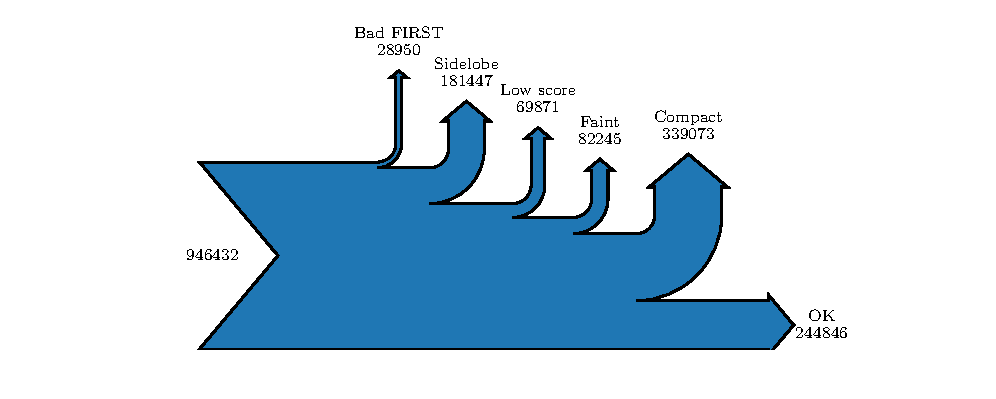
\includegraphics{rlf-images/sankey_components.pdf}
        \caption{\label{fig:sankey-components} \DIFaddFL{Number of components removed from FIRST by each filter.}}
    \end{figure}

    \begin{figure}
        \centering
        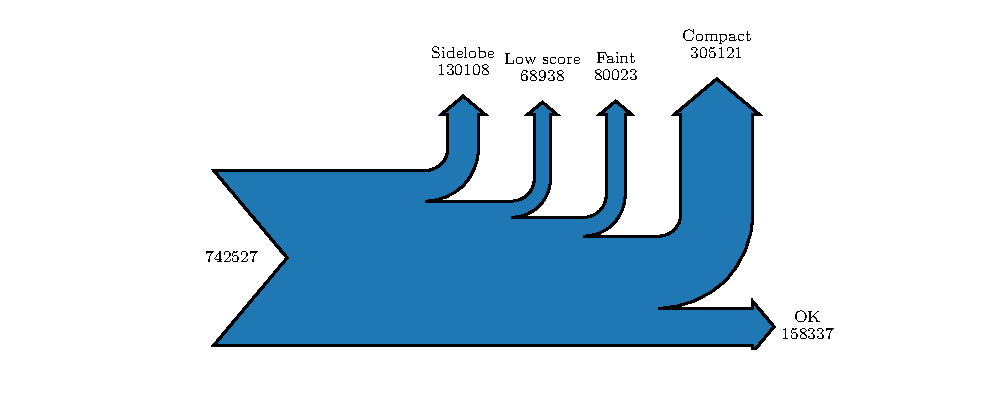
\includegraphics{rlf-images/sankey_sources.pdf}
        \caption{\label{fig:sankey-sources} \DIFaddFL{Number of sources removed by each filter.}}
    \end{figure}

\section{\DIFadd{Visual verification results}}
\label{sec:rlfs-verification-appendix}

  \DIFadd{In }\autoref{sec:rlfs-manual-validation} \DIFadd{we described our visual verification of the BXID method. We list the radio components in the verification set in }\autoref{tab:verification-set}\DIFadd{. Each row of the table contains the FIRST component, its All}\emph{\DIFadd{WISE}} \DIFadd{host galaxy according to BXID, and whether the association is correct according to our visual verification. If a verifier was particularly unsure about an object, they were able to skip this object, and so are not accounted for in the verification for that object. Verification was weighted by the \mbox{%DIFAUXCMD
\citet{dawid79em} }\hspace{0pt}%DIFAUXCMD
maximum likelihood model.
}

  \begin{table}
    \caption[Validation objects.]{\label{tab:verification-set} \DIFaddFL{Validation objects. `Agree' is whether or not the verifiers agreed with BXID associating the given FIRST object with the given All}\emph{\DIFaddFL{WISE}} \DIFaddFL{object.}}
        \scriptsize\centering
      \begin{tabular}{ccc}
        \hline\hline
        \DIFaddFL{FIRST }& \DIFaddFL{All}\emph{\DIFaddFL{WISE}} & \DIFaddFL{Agree}\\\hline
        \DIFaddFL{J000234.9-001421 }& \DIFaddFL{J000242.35-001320.5 }& \DIFaddFL{n}\\
        \DIFaddFL{J002841.1+141654 }& \DIFaddFL{J002840.37+141652.7 }& \DIFaddFL{y}\\
        \DIFaddFL{J003731.4+000156 }& \DIFaddFL{J003731.26+000146.7 }& \DIFaddFL{y}\\
        \DIFaddFL{J005407.5-011158 }& \DIFaddFL{J005407.61-011158.9 }& \DIFaddFL{y}\\
        \DIFaddFL{J011210.3+002203 }& \DIFaddFL{J011210.41+002201.9 }& \DIFaddFL{y}\\
        \DIFaddFL{J012342.4+015849 }& \DIFaddFL{J012342.24+015850.4 }& \DIFaddFL{y}\\
        \DIFaddFL{J013015.1+110653 }& \DIFaddFL{J013015.16+110653.4 }& \DIFaddFL{y}\\
        \DIFaddFL{J013107.7+070343 }& \DIFaddFL{J013102.02+070332.0 }& \DIFaddFL{y}\\
        \DIFaddFL{J014247.9-000039 }& \DIFaddFL{J014247.81-000040.3 }& \DIFaddFL{y}\\
        \DIFaddFL{J014250.0-000032 }& \DIFaddFL{J014247.81-000040.3 }& \DIFaddFL{n}\\
        \DIFaddFL{J020222.3+030138 }& \DIFaddFL{J020223.20+030150.4 }& \DIFaddFL{y}\\
        \DIFaddFL{J020333.8+000853 }& \DIFaddFL{J020336.94+000759.3 }& \DIFaddFL{y}\\
        \DIFaddFL{J021840.1-032311 }& \DIFaddFL{J021840.13-032306.0 }& \DIFaddFL{y}\\
        \DIFaddFL{J023022.0+010834 }& \DIFaddFL{J023022.11+010840.0 }& \DIFaddFL{y}\\
        \DIFaddFL{J024245.3-022535 }& \DIFaddFL{J024245.35-022534.6 }& \DIFaddFL{y}\\
        \DIFaddFL{J025901.0+005350 }& \DIFaddFL{J025901.50+005346.1 }& \DIFaddFL{y}\\
        \DIFaddFL{J033204.1-004757 }& \DIFaddFL{J033204.15-004757.1 }& \DIFaddFL{y}\\
        \DIFaddFL{J073033.2+390413 }& \DIFaddFL{J073033.21+390412.9 }& \DIFaddFL{y}\\
        \DIFaddFL{J073954.1+481810 }& \DIFaddFL{J073954.87+481759.5 }& \DIFaddFL{y}\\
        \DIFaddFL{J074504.9+331247 }& \DIFaddFL{J074504.81+331256.2 }& \DIFaddFL{y}\\
        \DIFaddFL{J074640.4+421709 }& \DIFaddFL{J074640.45+421709.1 }& \DIFaddFL{y}\\
        \DIFaddFL{J074707.9+171719 }& \DIFaddFL{J074708.35+171726.5 }& \DIFaddFL{y}\\
        \DIFaddFL{J075043.6+274838 }& \DIFaddFL{J075043.35+274844.8 }& \DIFaddFL{n}\\
        \DIFaddFL{J075050.3+331937 }& \DIFaddFL{J075051.25+331905.0 }& \DIFaddFL{y}\\
        \DIFaddFL{J075422.2+311253 }& \DIFaddFL{J075422.35+311252.5 }& \DIFaddFL{y}\\
        \DIFaddFL{J075637.0+212006 }& \DIFaddFL{J075636.65+212001.4 }& \DIFaddFL{y}\\
        \DIFaddFL{J082326.1+141438 }& \DIFaddFL{J082326.34+141435.9 }& \DIFaddFL{y}\\
        \DIFaddFL{J082422.5+351121 }& \DIFaddFL{J082422.65+351114.6 }& \DIFaddFL{y}\\
        \DIFaddFL{J082925.9+462618 }& \DIFaddFL{J082926.02+462618.5 }& \DIFaddFL{y}\\
        \DIFaddFL{J083512.4+175441 }& \DIFaddFL{J083512.45+175441.1 }& \DIFaddFL{y}\\
        \DIFaddFL{J084133.5+402035 }& \DIFaddFL{J084133.40+402042.8 }& \DIFaddFL{y}\\
        \DIFaddFL{J084238.4+405305 }& \DIFaddFL{J084238.38+405306.6 }& \DIFaddFL{n}\\
        \DIFaddFL{J084417.3+315845 }& \DIFaddFL{J084417.92+315845.9 }& \DIFaddFL{y}\\
        \DIFaddFL{J084728.5+360700 }& \DIFaddFL{J084728.24+360714.6 }& \DIFaddFL{y}\\
        \DIFaddFL{J084905.5+111448 }& \DIFaddFL{J084905.51+111447.8 }& \DIFaddFL{y}\\
        \DIFaddFL{J085236.8+262006 }& \DIFaddFL{J085236.11+262013.4 }& \DIFaddFL{y}\\
        \DIFaddFL{J085415.6+524930 }& \DIFaddFL{J085415.62+524936.7 }& \DIFaddFL{y}\\
        \DIFaddFL{J090623.2+300746 }& \DIFaddFL{J090622.87+300743.9 }& \DIFaddFL{y}\\
        \DIFaddFL{J091745.1+275049 }& \DIFaddFL{J091745.89+275103.8 }& \DIFaddFL{y}\\
        \DIFaddFL{J091752.0+431614 }& \DIFaddFL{J091752.14+431612.7 }& \DIFaddFL{y}\\
        \DIFaddFL{J092014.4+302907 }& \DIFaddFL{J092013.95+302859.3 }& \DIFaddFL{y}\\
        \DIFaddFL{J092140.5+540118 }& \DIFaddFL{J092140.24+540121.1 }& \DIFaddFL{y}\\
        \DIFaddFL{J092213.0+542157 }& \DIFaddFL{J092213.03+542157.2 }& \DIFaddFL{y}\\
        \DIFaddFL{J092406.9+562703 }& \DIFaddFL{J092406.47+562656.2 }& \DIFaddFL{y}\\
        \DIFaddFL{J092713.1+105841 }& \DIFaddFL{J092713.14+105839.8 }& \DIFaddFL{y}\\
        \DIFaddFL{J093108.6+613447 }& \DIFaddFL{J093108.63+613447.2 }& \DIFaddFL{y}\\
        \DIFaddFL{J093239.6+052308 }& \DIFaddFL{J093237.71+052240.7 }& \DIFaddFL{n}\\
        \DIFaddFL{J093627.8+103610 }& \DIFaddFL{J093627.87+103609.7 }& \DIFaddFL{y}\\
        \DIFaddFL{J093645.2+561435 }& \DIFaddFL{J093645.89+561434.2 }& \DIFaddFL{y}\\
        \DIFaddFL{J094006.8+482651 }& \DIFaddFL{J094006.92+482649.2 }& \DIFaddFL{y}\\\hline\hline
  \end{tabular}
  \begin{tabular}{ccc}
        \hline\hline
        \DIFaddFL{FIRST }& \DIFaddFL{All}\emph{\DIFaddFL{WISE}} & \DIFaddFL{Agree}\\\hline
        \DIFaddFL{J094009.5+600403 }& \DIFaddFL{J094011.55+600357.6 }& \DIFaddFL{n}\\
        \DIFaddFL{J094023.7+135123 }& \DIFaddFL{J094023.73+135125.2 }& \DIFaddFL{y}\\
        \DIFaddFL{J094324.5+435341 }& \DIFaddFL{J094324.61+435342.0 }& \DIFaddFL{y}\\
        \DIFaddFL{J094650.8+382015 }& \DIFaddFL{J094650.44+382010.9 }& \DIFaddFL{y}\\
        \DIFaddFL{J095011.8+455319 }& \DIFaddFL{J095011.82+455320.0 }& \DIFaddFL{y}\\
        \DIFaddFL{J095113.5+180211 }& \DIFaddFL{J095113.82+180204.2 }& \DIFaddFL{n}\\
        \DIFaddFL{J095242.4+222638 }& \DIFaddFL{J095242.45+222638.0 }& \DIFaddFL{y}\\
        \DIFaddFL{J095538.7+013546 }& \DIFaddFL{J095539.20+013546.1 }& \DIFaddFL{y}\\
        \DIFaddFL{J095609.9+363441 }& \DIFaddFL{J095609.30+363445.4 }& \DIFaddFL{y}\\
        \DIFaddFL{J095811.8+225056 }& \DIFaddFL{J095811.90+225055.5 }& \DIFaddFL{y}\\
        \DIFaddFL{J100019.2+263516 }& \DIFaddFL{J100018.84+263527.5 }& \DIFaddFL{y}\\
        \DIFaddFL{J101315.9+064520 }& \DIFaddFL{J101316.51+064519.0 }& \DIFaddFL{y}\\
        \DIFaddFL{J101455.2-004716 }& \DIFaddFL{J101455.30-004718.3 }& \DIFaddFL{y}\\
        \DIFaddFL{J102153.5+260429 }& \DIFaddFL{J102153.52+260429.6 }& \DIFaddFL{y}\\
        \DIFaddFL{J102354.7+390653 }& \DIFaddFL{J102354.88+390654.0 }& \DIFaddFL{y}\\
        \DIFaddFL{J102620.4+303600 }& \DIFaddFL{J102620.46+303550.4 }& \DIFaddFL{y}\\
        \DIFaddFL{J102710.4+460254 }& \DIFaddFL{J102714.81+460256.4 }& \DIFaddFL{n}\\
        \DIFaddFL{J102955.9+424906 }& \DIFaddFL{J102955.96+424906.7 }& \DIFaddFL{y}\\
        \DIFaddFL{J103503.9+102404 }& \DIFaddFL{J103503.92+102403.6 }& \DIFaddFL{y}\\
        \DIFaddFL{J103839.9+331200 }& \DIFaddFL{J103839.94+331201.1 }& \DIFaddFL{y}\\
        \DIFaddFL{J104030.5+211624 }& \DIFaddFL{J104031.09+211620.6 }& \DIFaddFL{n}\\
        \DIFaddFL{J104533.8+430025 }& \DIFaddFL{J104535.22+430020.8 }& \DIFaddFL{y}\\
        \DIFaddFL{J104907.5+322903 }& \DIFaddFL{J104907.91+322906.6 }& \DIFaddFL{y}\\
        \DIFaddFL{J105146.9+552257 }& \DIFaddFL{J105147.40+552308.4 }& \DIFaddFL{y}\\
        \DIFaddFL{J105257.5+105418 }& \DIFaddFL{J105257.53+105421.5 }& \DIFaddFL{y}\\
        \DIFaddFL{J105521.6+372641 }& \DIFaddFL{J105521.24+372652.4 }& \DIFaddFL{y}\\
        \DIFaddFL{J105758.8+321605 }& \DIFaddFL{J105758.84+321605.3 }& \DIFaddFL{y}\\
        \DIFaddFL{J110104.9+151618 }& \DIFaddFL{J110104.90+151618.2 }& \DIFaddFL{y}\\
        \DIFaddFL{J110353.2+352320 }& \DIFaddFL{J110353.37+352319.9 }& \DIFaddFL{y}\\
        \DIFaddFL{J110414.4+481345 }& \DIFaddFL{J110423.08+481311.0 }& \DIFaddFL{n}\\
        \DIFaddFL{J111057.7+220756 }& \DIFaddFL{J111057.18+220758.3 }& \DIFaddFL{y}\\
        \DIFaddFL{J111208.5+275207 }& \DIFaddFL{J111201.79+275053.8 }& \DIFaddFL{n}\\
        \DIFaddFL{J111225.2+233159 }& \DIFaddFL{J111225.30+233157.9 }& \DIFaddFL{y}\\
        \DIFaddFL{J111726.3+375336 }& \DIFaddFL{J111726.35+375337.0 }& \DIFaddFL{y}\\
        \DIFaddFL{J111746.1+261151 }& \DIFaddFL{J111746.18+261150.9 }& \DIFaddFL{y}\\
        \DIFaddFL{J111854.3+424708 }& \DIFaddFL{J111854.45+424652.8 }& \DIFaddFL{y}\\
        \DIFaddFL{J112124.4+640417 }& \DIFaddFL{J112125.02+640408.6 }& \DIFaddFL{y}\\
        \DIFaddFL{J112135.3+352330 }& \DIFaddFL{J112135.44+352324.9 }& \DIFaddFL{y}\\
        \DIFaddFL{J112550.9+200631 }& \DIFaddFL{J112558.75+200554.3 }& \DIFaddFL{y}\\
        \DIFaddFL{J112859.7+260923 }& \DIFaddFL{J112859.86+260911.3 }& \DIFaddFL{y}\\
        \DIFaddFL{J113201.1+442639 }& \DIFaddFL{J113201.23+442639.4 }& \DIFaddFL{y}\\
        \DIFaddFL{J113302.5+355408 }& \DIFaddFL{J113301.80+355415.3 }& \DIFaddFL{y}\\
        \DIFaddFL{J113712.7+263301 }& \DIFaddFL{J113711.86+263335.1 }& \DIFaddFL{y}\\
        \DIFaddFL{J113756.3+471314 }& \DIFaddFL{J113756.31+471314.1 }& \DIFaddFL{y}\\
        \DIFaddFL{J113906.6+230602 }& \DIFaddFL{J113906.68+230602.1 }& \DIFaddFL{y}\\
        \DIFaddFL{J114325.0+600721 }& \DIFaddFL{J114323.90+600737.1 }& \DIFaddFL{y}\\
        \DIFaddFL{J114759.7+370305 }& \DIFaddFL{J114759.22+370311.2 }& \DIFaddFL{y}\\
        \DIFaddFL{J114916.7+083022 }& \DIFaddFL{J114916.33+083040.5 }& \DIFaddFL{n}\\
        \DIFaddFL{J115010.9+063340 }& \DIFaddFL{J115010.93+063340.5 }& \DIFaddFL{y}\\
        \DIFaddFL{J115308.6+374851 }& \DIFaddFL{J115316.96+374850.0 }& \DIFaddFL{y}\\\hline\hline
  \end{tabular}
\end{table}
\begin{table}
    \scriptsize\centering
  \begin{tabular}{ccc}
        \hline\hline
        \DIFaddFL{FIRST }& \DIFaddFL{All}\emph{\DIFaddFL{WISE}} & \DIFaddFL{Agree}\\\hline
        \DIFaddFL{J115448.7+472222 }& \DIFaddFL{J115448.67+472223.7 }& \DIFaddFL{y}\\
        \DIFaddFL{J115603.7+584704 }& \DIFaddFL{J115603.48+584706.1 }& \DIFaddFL{y}\\
        \DIFaddFL{J115605.9+343230 }& \DIFaddFL{J115605.64+343229.4 }& \DIFaddFL{y}\\
        \DIFaddFL{J115653.0+572338 }& \DIFaddFL{J115645.38+572151.7 }& \DIFaddFL{y}\\
        \DIFaddFL{J120138.0+230922 }& \DIFaddFL{J120137.97+230922.2 }& \DIFaddFL{y}\\
        \DIFaddFL{J120752.8+533808 }& \DIFaddFL{J120752.85+533807.3 }& \DIFaddFL{y}\\
        \DIFaddFL{J120943.3-021934 }& \DIFaddFL{J120942.89-021943.0 }& \DIFaddFL{y}\\
        \DIFaddFL{J121045.6+190225 }& \DIFaddFL{J121045.68+190227.0 }& \DIFaddFL{y}\\
        \DIFaddFL{J121207.6+115412 }& \DIFaddFL{J121207.72+115413.8 }& \DIFaddFL{y}\\
        \DIFaddFL{J121211.3+485951 }& \DIFaddFL{J121211.86+485952.0 }& \DIFaddFL{y}\\
        \DIFaddFL{J121406.7+002634 }& \DIFaddFL{J121406.73+002635.0 }& \DIFaddFL{y}\\
        \DIFaddFL{J122518.0+350258 }& \DIFaddFL{J122517.85+350301.9 }& \DIFaddFL{y}\\
        \DIFaddFL{J122525.1+451530 }& \DIFaddFL{J122524.71+451508.5 }& \DIFaddFL{y}\\
        \DIFaddFL{J122640.9+430508 }& \DIFaddFL{J122640.82+430509.2 }& \DIFaddFL{y}\\
        \DIFaddFL{J123429.8+260107 }& \DIFaddFL{J123434.79+260134.3 }& \DIFaddFL{n}\\
        \DIFaddFL{J123633.1+100928 }& \DIFaddFL{J123633.12+100928.7 }& \DIFaddFL{y}\\
        \DIFaddFL{J124839.3+411522 }& \DIFaddFL{J124839.42+411522.3 }& \DIFaddFL{n}\\
        \DIFaddFL{J125129.2+551012 }& \DIFaddFL{J125128.76+551009.3 }& \DIFaddFL{y}\\
        \DIFaddFL{J130005.8+524801 }& \DIFaddFL{J130006.14+524803.0 }& \DIFaddFL{y}\\
        \DIFaddFL{J130132.1+511351 }& \DIFaddFL{J130132.32+511352.5 }& \DIFaddFL{y}\\
        \DIFaddFL{J131104.4+464936 }& \DIFaddFL{J131104.45+464934.0 }& \DIFaddFL{y}\\
        \DIFaddFL{J131452.2+252811 }& \DIFaddFL{J131446.81+252820.8 }& \DIFaddFL{n}\\
        \DIFaddFL{J132033.8+332639 }& \DIFaddFL{J132033.59+332639.0 }& \DIFaddFL{n}\\
        \DIFaddFL{J132257.5+191134 }& \DIFaddFL{J132257.53+191133.9 }& \DIFaddFL{y}\\
        \DIFaddFL{J132529.3+230734 }& \DIFaddFL{J132529.35+230733.8 }& \DIFaddFL{y}\\
        \DIFaddFL{J132546.8+052453 }& \DIFaddFL{J132546.86+052454.1 }& \DIFaddFL{y}\\
        \DIFaddFL{J132637.7+112110 }& \DIFaddFL{J132637.92+112108.8 }& \DIFaddFL{y}\\
        \DIFaddFL{J132831.8+104339 }& \DIFaddFL{J132831.88+104338.8 }& \DIFaddFL{y}\\
        \DIFaddFL{J132932.3+131839 }& \DIFaddFL{J132932.32+131839.6 }& \DIFaddFL{y}\\
        \DIFaddFL{J133022.8+311904 }& \DIFaddFL{J133022.83+311902.8 }& \DIFaddFL{y}\\
        \DIFaddFL{J133453.3+405653 }& \DIFaddFL{J133454.13+405650.6 }& \DIFaddFL{y}\\
        \DIFaddFL{J133741.1+124302 }& \DIFaddFL{J133741.13+124303.1 }& \DIFaddFL{y}\\
        \DIFaddFL{J133823.6+103337 }& \DIFaddFL{J133823.67+103341.9 }& \DIFaddFL{y}\\
        \DIFaddFL{J134651.2+415154 }& \DIFaddFL{J134651.06+415156.1 }& \DIFaddFL{y}\\
        \DIFaddFL{J134704.3+110622 }& \DIFaddFL{J134704.35+110622.7 }& \DIFaddFL{y}\\
        \DIFaddFL{J134752.7+555046 }& \DIFaddFL{J134752.71+555048.6 }& \DIFaddFL{y}\\
        \DIFaddFL{J134831.7+164325 }& \DIFaddFL{J134831.57+164328.2 }& \DIFaddFL{y}\\
        \DIFaddFL{J134949.8+385539 }& \DIFaddFL{J134949.93+385542.8 }& \DIFaddFL{y}\\
        \DIFaddFL{J135106.5+074534 }& \DIFaddFL{J135106.50+074534.2 }& \DIFaddFL{y}\\
        \DIFaddFL{J135107.7+615502 }& \DIFaddFL{J135107.75+615502.1 }& \DIFaddFL{y}\\
        \DIFaddFL{J135658.5+134028 }& \DIFaddFL{J135659.15+134017.0 }& \DIFaddFL{y}\\
        \DIFaddFL{J135833.9+180021 }& \DIFaddFL{J135834.03+180020.4 }& \DIFaddFL{y}\\
        \DIFaddFL{J140630.7+554017 }& \DIFaddFL{J140629.32+554009.9 }& \DIFaddFL{y}\\
        \DIFaddFL{J140804.2+503019 }& \DIFaddFL{J140804.10+503021.1 }& \DIFaddFL{y}\\
        \DIFaddFL{J141226.7+454125 }& \DIFaddFL{J141226.54+454125.5 }& \DIFaddFL{y}\\
        \DIFaddFL{J141245.0+495213 }& \DIFaddFL{J141243.84+495206.4 }& \DIFaddFL{y}\\
        \DIFaddFL{J141317.4+325306 }& \DIFaddFL{J141317.50+325306.8 }& \DIFaddFL{y}\\
        \DIFaddFL{J141723.8+543639 }& \DIFaddFL{J141724.33+543629.5 }& \DIFaddFL{y}\\
        \DIFaddFL{J141938.8+312146 }& \DIFaddFL{J141940.16+312138.8 }& \DIFaddFL{y}\\
        \DIFaddFL{J142515.3+175526 }& \DIFaddFL{J142513.89+175525.7 }& \DIFaddFL{y}\\\hline\hline
  \end{tabular}
  \begin{tabular}{ccc}
        \hline\hline
        \DIFaddFL{FIRST }& \DIFaddFL{All}\emph{\DIFaddFL{WISE}} & \DIFaddFL{Agree}\\\hline
        \DIFaddFL{J142829.5+070836 }& \DIFaddFL{J142829.60+070836.3 }& \DIFaddFL{y}\\
        \DIFaddFL{J143411.0+170036 }& \DIFaddFL{J143411.18+170035.7 }& \DIFaddFL{y}\\
        \DIFaddFL{J143624.0-001057 }& \DIFaddFL{J143623.89-001100.8 }& \DIFaddFL{y}\\
        \DIFaddFL{J143742.6+104412 }& \DIFaddFL{J143742.69+104412.8 }& \DIFaddFL{y}\\
        \DIFaddFL{J143840.8+475355 }& \DIFaddFL{J143841.08+475356.1 }& \DIFaddFL{y}\\
        \DIFaddFL{J143909.1+430847 }& \DIFaddFL{J143909.08+430847.8 }& \DIFaddFL{y}\\
        \DIFaddFL{J144135.8+102246 }& \DIFaddFL{J144135.91+102245.1 }& \DIFaddFL{y}\\
        \DIFaddFL{J144333.6+275229 }& \DIFaddFL{J144333.02+275250.2 }& \DIFaddFL{y}\\
        \DIFaddFL{J145012.3+471739 }& \DIFaddFL{J145012.33+471738.7 }& \DIFaddFL{y}\\
        \DIFaddFL{J145103.7+452459 }& \DIFaddFL{J145102.66+452520.5 }& \DIFaddFL{n}\\
        \DIFaddFL{J145401.6+141009 }& \DIFaddFL{J145401.70+141009.6 }& \DIFaddFL{y}\\
        \DIFaddFL{J150158.7+191413 }& \DIFaddFL{J150158.87+191405.3 }& \DIFaddFL{y}\\
        \DIFaddFL{J150743.9+352720 }& \DIFaddFL{J150743.62+352724.1 }& \DIFaddFL{y}\\
        \DIFaddFL{J151141.6-003209 }& \DIFaddFL{J151142.01-003213.0 }& \DIFaddFL{y}\\
        \DIFaddFL{J151315.5+403107 }& \DIFaddFL{J151315.56+403107.7 }& \DIFaddFL{y}\\
        \DIFaddFL{J151518.7+230256 }& \DIFaddFL{J151518.67+230257.3 }& \DIFaddFL{y}\\
        \DIFaddFL{J151703.6+105947 }& \DIFaddFL{J151703.68+105947.6 }& \DIFaddFL{y}\\
        \DIFaddFL{J151736.8+610856 }& \DIFaddFL{J151736.83+610857.7 }& \DIFaddFL{y}\\
        \DIFaddFL{J152121.6+281635 }& \DIFaddFL{J152120.68+281626.2 }& \DIFaddFL{y}\\
        \DIFaddFL{J152714.8+310425 }& \DIFaddFL{J152714.88+310424.7 }& \DIFaddFL{y}\\
        \DIFaddFL{J153428.9+272134 }& \DIFaddFL{J153429.68+272120.8 }& \DIFaddFL{y}\\
        \DIFaddFL{J154245.3+100919 }& \DIFaddFL{J154245.71+100917.8 }& \DIFaddFL{y}\\
        \DIFaddFL{J154901.6+103159 }& \DIFaddFL{J154901.40+103152.6 }& \DIFaddFL{y}\\
        \DIFaddFL{J154925.2+395316 }& \DIFaddFL{J154926.17+395303.7 }& \DIFaddFL{y}\\
        \DIFaddFL{J155206.3-005348 }& \DIFaddFL{J155206.58-005339.3 }& \DIFaddFL{y}\\
        \DIFaddFL{J155457.3+344637 }& \DIFaddFL{J155458.45+344644.7 }& \DIFaddFL{y}\\
        \DIFaddFL{J155743.5+272752 }& \DIFaddFL{J155743.52+272752.8 }& \DIFaddFL{y}\\
        \DIFaddFL{J160130.0+083848 }& \DIFaddFL{J160130.07+083850.7 }& \DIFaddFL{y}\\
        \DIFaddFL{J160534.8+441220 }& \DIFaddFL{J160535.55+441221.5 }& \DIFaddFL{y}\\
        \DIFaddFL{J160859.2+400135 }& \DIFaddFL{J160901.32+400230.7 }& \DIFaddFL{n}\\
        \DIFaddFL{J161545.4+231617 }& \DIFaddFL{J161545.14+231617.2 }& \DIFaddFL{y}\\
        \DIFaddFL{J161930.4+085533 }& \DIFaddFL{J161930.51+085532.6 }& \DIFaddFL{y}\\
        \DIFaddFL{J162228.0+264743 }& \DIFaddFL{J162228.70+264736.7 }& \DIFaddFL{y}\\
        \DIFaddFL{J162750.4+473624 }& \DIFaddFL{J162750.55+473623.5 }& \DIFaddFL{y}\\
        \DIFaddFL{J162904.2+470852 }& \DIFaddFL{J162904.34+470853.0 }& \DIFaddFL{y}\\
        \DIFaddFL{J163038.7+214740 }& \DIFaddFL{J163037.43+214748.9 }& \DIFaddFL{n}\\
        \DIFaddFL{J163323.6+424051 }& \DIFaddFL{J163323.61+424051.9 }& \DIFaddFL{y}\\
        \DIFaddFL{J163327.5+242426 }& \DIFaddFL{J163327.87+242427.4 }& \DIFaddFL{y}\\
        \DIFaddFL{J163533.8+454557 }& \DIFaddFL{J163534.00+454554.3 }& \DIFaddFL{y}\\
        \DIFaddFL{J164211.2+512029 }& \DIFaddFL{J164211.27+512029.3 }& \DIFaddFL{y}\\
        \DIFaddFL{J165549.1+375923 }& \DIFaddFL{J165549.01+375923.6 }& \DIFaddFL{y}\\
        \DIFaddFL{J165620.0+363402 }& \DIFaddFL{J165619.89+363403.9 }& \DIFaddFL{y}\\
        \DIFaddFL{J165700.5+474820 }& \DIFaddFL{J165659.58+474809.0 }& \DIFaddFL{y}\\
        \DIFaddFL{J171406.2+292712 }& \DIFaddFL{J171404.16+292704.0 }& \DIFaddFL{n}\\
        \DIFaddFL{J172126.4+374446 }& \DIFaddFL{J172126.46+374446.6 }& \DIFaddFL{y}\\
        \DIFaddFL{J222627.7-005010 }& \DIFaddFL{J222627.77-005010.8 }& \DIFaddFL{y}\\
        \DIFaddFL{J223636.4-013827 }& \DIFaddFL{J223636.48-013827.2 }& \DIFaddFL{y}\\
        \DIFaddFL{J225619.0+143257 }& \DIFaddFL{J225621.96+143351.4 }& \DIFaddFL{y}\\
        \DIFaddFL{J232410.1+001315 }& \DIFaddFL{J232410.15+001314.5 }& \DIFaddFL{y}\\
        \DIFaddFL{J234727.9-000919 }& \DIFaddFL{J234727.65-000912.9 }& \DIFaddFL{y}\\\hline\hline
  \end{tabular}
\end{table}

\section{\DIFadd{Radio luminosity function}}
\label{sec:rlfs-rlf-desc}

  \DIFadd{We computed the radio luminosity function following the $1/V_{\max}$ method
  \mbox{%DIFAUXCMD
\citep{schmidt1968vmax}}\hspace{0pt}%DIFAUXCMD
. We performed the
  following steps:
  }\begin{enumerate}
    \item \DIFadd{Remove all radio sources that do not fit the selection criteria.
      This applies for both radio and infrared properties, so we choose a minimum radio flux density $f_{\min}$ and a maximum infrared magnitude
      $m_{\max,\text{ir}}$, as well as redshift limits $z_{\mathrm{lower}}$ and $z_{\mathrm{upper}}$.
    }\item \DIFadd{For each source, compute the maximum redshift that the source could
      have been observed within the selection criteria. We find this redshift
      by first numerically solving }\autoref{eq:luminosity} \DIFadd{for $z$ with $L$ as
      the luminosity of each radio source and $f = f_{\min}$ to obtain the
      maximum redshift $z_\text{radio}$ at which the source could be observed
      in radio. We similarly find the maximum redshift that the infrared host
      galaxy could be observed at within the selection criteria, $z_{\text{ir}}$, by numerically
      solving }\autoref{eq:ir-limits}\DIFadd{. $d(z_{\text{ir}})$ is the luminosity
      distance at a redshift $z_{\text{ir}}$, $d$ is the luminosity distance of the host
      galaxy, and $m$ is the apparent magnitude of the host galaxy, all in the infrared.
      }\begin{equation}
        \DIFadd{\label{eq:ir-limits}
        5 \log_{10}\left(\frac{d(z_{\text{ir}})}{d}\right) + m = m_{\max,\text{ir}}
      }\end{equation}
      \DIFadd{The maximum redshift that the source could have been observed within the
      selection criteria is then $z_{\mathrm{max}} = \min(z_{\mathrm{ir}}, z_{\mathrm{radio}}, z_{\mathrm{upper}})$.
    }\item \DIFadd{For each source, compute the comoving volume $V_{\mathrm{max}}$ at
      redshift $z_{\mathrm{max}}$.
    }\item \DIFadd{The count for each luminosity bin is the sum over $1 / V_{\max}$ for
      each source in the bin. We divide these counts by the estimated completeness (}\aref{sec:rlfs-completeness}\DIFadd{) to account for redshift incompleteness.
      We account for the fact FIRST does not cover the
      whole sky by multiplying by the total area of the sky divided by the area
      of our selection.
  }\end{enumerate}

  \DIFadd{After computing the luminosity function, we estimate the uncertainty in each bin using Poisson statistics, $\sqrt{N}$ for a bin count $N$.
}

  \section{\DIFadd{Redshift completeness estimate}}
  \label{sec:rlfs-completeness}

    \autoref{fig:completeness-wise} \DIFadd{shows the estimated completeness of our RLF sample in }\autoref{cha:rlfs} \DIFadd{as a function of $W1$ and $W1-W2$. We followed the same method as \mbox{%DIFAUXCMD
\citet{pracy16rlf} }\hspace{0pt}%DIFAUXCMD
for this estimation, averaging completeness over circles centred on each source. Each source is associated with a circle of radius equal to the distance to its 50th nearest neighbour in the $W1$ and $W1-W2$ plane. This appendix was originally part of \mbox{%DIFAUXCMD
\citet{alger21rlfs}}\hspace{0pt}%DIFAUXCMD
.
}

    \begin{figure}
        \centering
        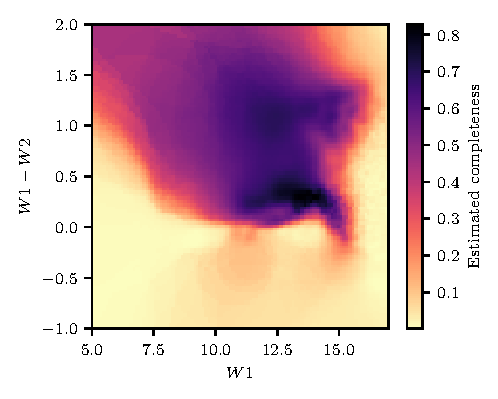
\includegraphics{rlf-images/completeness_wise.pdf}
        \caption{\label{fig:completeness-wise} \DIFaddFL{Estimated completeness as a function of mid-infrared colour and magnitude.}}
    \end{figure}

  \section{\DIFadd{Giant radio galaxies}}
  \label{sec:rlfs-giants}

    \begin{table*}
      \caption[Giant radio galaxies found in RGZ-Ex.]{\label{tab:grg} \DIFaddFL{Giant radio galaxies found in RGZ-Ex. `LLS' is the projected linear size of the source as measured by the maximum angular distance between radio components. The RA/Dec are the coordinates of the host galaxy. s/p indicates spectroscopic/photometric redshift. ${}^L$Existing in literature. ${}^R$Also found by RGZ citizen scientists. ${}^\dagger$Misidentified SDSS host, manually corrected to obtain redshift.}}
      \centering
      \begin{footnotesize}\begin{tabular}{c|ccccc}
  \hline\hline
  \DIFaddFL{All}\emph{\DIFaddFL{WISE}} \DIFaddFL{host (WISEA) }& \DIFaddFL{RA (J2000) }& \DIFaddFL{Dec (J2000) }& \DIFaddFL{$z$ }& \DIFaddFL{LLS (Mpc) }&\\
  \hline
    \DIFaddFL{J004210.18-080011.3 }& \DIFaddFL{10.54 }& \DIFaddFL{-8.00 }& \DIFaddFL{$0.65 \pm 0.14$ }& \DIFaddFL{1.6 }& \DIFaddFL{p}\\ %DIF >  3051
    \DIFaddFL{J021008.48+011839.6${}^L$ }& \DIFaddFL{32.54 }& \DIFaddFL{1.31 }& \DIFaddFL{$0.86524 \pm 0.0001$ }& \DIFaddFL{1.2 }& \DIFaddFL{s}\\ %DIF >  8420
    \DIFaddFL{J075858.29+355643.6${}^R$ }& \DIFaddFL{119.74 }& \DIFaddFL{35.95 }& \DIFaddFL{$0.74748 \pm 0.00013$ }& \DIFaddFL{1.0 }& \DIFaddFL{s}\\ %DIF >  19661
    \DIFaddFL{J080831.68+473523.9${}^R$ }& \DIFaddFL{122.13 }& \DIFaddFL{47.59 }& \DIFaddFL{$0.58854 \pm 0.00016$ }& \DIFaddFL{1.1 }& \DIFaddFL{s}\\ %DIF >  21331
    \DIFaddFL{J083034.78+231124.6 }& \DIFaddFL{127.64 }& \DIFaddFL{23.19 }& \DIFaddFL{$0.94 \pm 0.13$ }& \DIFaddFL{1.1 }& \DIFaddFL{p}\\ %DIF >  25768
    \DIFaddFL{J090604.03+011114.2 }& \DIFaddFL{136.52 }& \DIFaddFL{1.19 }& \DIFaddFL{$0.7975 \pm 0.0004$ }& \DIFaddFL{1.6 }& \DIFaddFL{s}\\ %DIF >  33696
    \DIFaddFL{J093256.81+074212.2 }& \DIFaddFL{143.24 }& \DIFaddFL{7.70 }& \DIFaddFL{$1.0032 \pm 0.0003$ }& \DIFaddFL{1.1 }& \DIFaddFL{s}\\ %DIF >  39983
    \DIFaddFL{J093526.80+051729.8${}^R$ }& \DIFaddFL{143.86 }& \DIFaddFL{5.29 }& \DIFaddFL{$0.84 \pm 0.04$ }& \DIFaddFL{1.2 }& \DIFaddFL{p}\\ %DIF >  40574
    \DIFaddFL{J094238.72+114337.9 }& \DIFaddFL{145.66 }& \DIFaddFL{11.73 }& \DIFaddFL{$0.49 \pm 0.05$ }& \DIFaddFL{1.2 }& \DIFaddFL{p}\\ %DIF >  42294
    \DIFaddFL{J094835.60+535946.4${}^R$ }& \DIFaddFL{147.15 }& \DIFaddFL{54.00 }& \DIFaddFL{$0.64 \pm 0.10$ }& \DIFaddFL{1.2 }& \DIFaddFL{p}\\ %DIF >  43609
    \DIFaddFL{J095706.12+292439.2 }& \DIFaddFL{149.28 }& \DIFaddFL{29.41 }& \DIFaddFL{$0.71 \pm 0.12$ }& \DIFaddFL{1.5 }& \DIFaddFL{p}\\ %DIF >  45638
    \DIFaddFL{J102335.25+433208.0 }& \DIFaddFL{155.90 }& \DIFaddFL{43.54 }& \DIFaddFL{$0.75 \pm 0.09$ }& \DIFaddFL{1.5 }& \DIFaddFL{p}\\ %DIF >  51758
    \DIFaddFL{J102933.99+210345.8${}^R$ }& \DIFaddFL{157.39 }& \DIFaddFL{21.06 }& \DIFaddFL{$0.82407 \pm 0.00008$ }& \DIFaddFL{1.1 }& \DIFaddFL{s}\\ %DIF >  53159
    \DIFaddFL{J103043.98+355451.2${}^R$ }& \DIFaddFL{157.68 }& \DIFaddFL{35.91 }& \DIFaddFL{$0.64074 \pm 0.00008$ }& \DIFaddFL{1.2 }& \DIFaddFL{s}\\ %DIF >  53433
    \DIFaddFL{J104449.92+234525.6${}^\dagger$ }& \DIFaddFL{161.20 }& \DIFaddFL{23.76 }& \DIFaddFL{$0.57712 \pm 0.00009$ }& \DIFaddFL{1.6 }& \DIFaddFL{s}\\ %DIF >  56652
    \DIFaddFL{J110655.98+624759.8${}^R$ }& \DIFaddFL{166.73 }& \DIFaddFL{62.80 }& \DIFaddFL{$0.84379 \pm 0.00004$ }& \DIFaddFL{1.1 }& \DIFaddFL{s}\\ %DIF >  61882
    \DIFaddFL{J112900.68+635543.2 }& \DIFaddFL{172.25 }& \DIFaddFL{63.93 }& \DIFaddFL{$0.71 \pm 0.06$ }& \DIFaddFL{1.1 }& \DIFaddFL{p}\\ %DIF >  67101
    \DIFaddFL{J112948.20+243922.6 }& \DIFaddFL{172.45 }& \DIFaddFL{24.66 }& \DIFaddFL{$0.79 \pm 0.07$ }& \DIFaddFL{1.1 }& \DIFaddFL{p}\\ %DIF >  67288
    \DIFaddFL{J114553.67-003304.7 }& \DIFaddFL{176.47 }& \DIFaddFL{-0.55 }& \DIFaddFL{$2.0522 \pm 0.0006$ }& \DIFaddFL{1.3 }& \DIFaddFL{s}\\ %DIF >  71048
    \DIFaddFL{J121111.26+534840.4 }& \DIFaddFL{182.80 }& \DIFaddFL{53.81 }& \DIFaddFL{$0.74 \pm 0.14$ }& \DIFaddFL{1.1 }& \DIFaddFL{p}\\ %DIF >  77051
    \DIFaddFL{J121152.04+304232.4${}^R$ }& \DIFaddFL{182.97 }& \DIFaddFL{30.71 }& \DIFaddFL{$0.47102 \pm 0.00012$ }& \DIFaddFL{1.3 }& \DIFaddFL{s}\\ %DIF >  77229
    \DIFaddFL{J121944.73+174121.3 }& \DIFaddFL{184.94 }& \DIFaddFL{17.69 }& \DIFaddFL{$1.5129 \pm 0.0009$ }& \DIFaddFL{1.0 }& \DIFaddFL{s}\\ %DIF >  79128
    \DIFaddFL{J123735.89+544814.4${}^R$ }& \DIFaddFL{189.40 }& \DIFaddFL{54.80 }& \DIFaddFL{$1.0271 \pm 0.0006$ }& \DIFaddFL{1.2 }& \DIFaddFL{s}\\ %DIF >  83169
    \DIFaddFL{J123819.16+113444.8 }& \DIFaddFL{189.58 }& \DIFaddFL{11.58 }& \DIFaddFL{$0.80 \pm 0.08$ }& \DIFaddFL{1.2 }& \DIFaddFL{p}\\ %DIF >  83310
    \DIFaddFL{J123846.84-032857.5${}^\dagger$ }& \DIFaddFL{189.70 }& \DIFaddFL{-3.48 }& \DIFaddFL{$0.67 \pm 0.07$ }& \DIFaddFL{1.5 }& \DIFaddFL{p}\\ %DIF >  83402
    \DIFaddFL{J131625.00+272042.8 }& \DIFaddFL{199.10 }& \DIFaddFL{27.35 }& \DIFaddFL{$0.69092 \pm 0.00004$ }& \DIFaddFL{1.0 }& \DIFaddFL{s}\\ %DIF >  92344
    \DIFaddFL{J133307.00+045048.6${}^R$ }& \DIFaddFL{203.28 }& \DIFaddFL{4.85 }& \DIFaddFL{$1.40534 \pm 0.00016$ }& \DIFaddFL{1.1 }& \DIFaddFL{s}\\ %DIF >  96197
    \DIFaddFL{J141933.36+104706.4${}^R$ }& \DIFaddFL{214.89 }& \DIFaddFL{10.79 }& \DIFaddFL{$0.33973 \pm 0.00003$ }& \DIFaddFL{1.0 }& \DIFaddFL{s}\\ %DIF >  107030
    \DIFaddFL{J142008.45+185422.7${}^R$ }& \DIFaddFL{215.04 }& \DIFaddFL{18.91 }& \DIFaddFL{$0.63 \pm 0.04$ }& \DIFaddFL{1.4 }& \DIFaddFL{p}\\ %DIF >  107197
    \DIFaddFL{J145057.28+530007.7${}^L$ }& \DIFaddFL{222.74 }& \DIFaddFL{53.00 }& \DIFaddFL{$0.91662 \pm 0.00009$ }& \DIFaddFL{1.3 }& \DIFaddFL{s}\\ %DIF >  114664
    \DIFaddFL{J150012.18+604941.3 }& \DIFaddFL{225.05 }& \DIFaddFL{60.83 }& \DIFaddFL{$1.6626 \pm 0.0007$ }& \DIFaddFL{1.2 }& \DIFaddFL{s}\\ %DIF >  116901
    \DIFaddFL{J153547.13+432245.0${}^R$ }& \DIFaddFL{233.95 }& \DIFaddFL{43.38 }& \DIFaddFL{$0.63891 \pm 0.00007$ }& \DIFaddFL{1.3 }& \DIFaddFL{s}\\ %DIF >  125394
    \DIFaddFL{J154631.18+194819.9 }& \DIFaddFL{236.63 }& \DIFaddFL{19.81 }& \DIFaddFL{$0.5917 \pm 0.0002$ }& \DIFaddFL{1.4 }& \DIFaddFL{s}\\ %DIF >  127907
    \DIFaddFL{J160852.10+561110.2${}^R$ }& \DIFaddFL{242.22 }& \DIFaddFL{56.19 }& \DIFaddFL{$1.3196 \pm 0.0003$ }& \DIFaddFL{1.3 }& \DIFaddFL{s}\\ %DIF >  132855
    \DIFaddFL{J162200.48+364044.0 }& \DIFaddFL{245.50 }& \DIFaddFL{36.68 }& \DIFaddFL{$1.9994 \pm 0.0002$ }& \DIFaddFL{1.1 }& \DIFaddFL{s}\\ %DIF >  135486
    \DIFaddFL{J163004.35+103321.9${}^R$ }& \DIFaddFL{247.52 }& \DIFaddFL{10.56 }& \DIFaddFL{$0.85 \pm 0.09$ }& \DIFaddFL{1.2 }& \DIFaddFL{p}\\ %DIF >  136997
    \DIFaddFL{J163125.75+200224.1${}^R$ }& \DIFaddFL{247.86 }& \DIFaddFL{20.04 }& \DIFaddFL{$0.62662 \pm 0.00013$ }& \DIFaddFL{1.0 }& \DIFaddFL{s}\\ %DIF >  137251
    \DIFaddFL{J165055.46+394446.6 }& \DIFaddFL{252.73 }& \DIFaddFL{39.75 }& \DIFaddFL{$0.58829 \pm 0.00013$ }& \DIFaddFL{1.1 }& \DIFaddFL{s}\\ %DIF >  140491
    \DIFaddFL{J232410.33+045309.6 }& \DIFaddFL{351.04 }& \DIFaddFL{4.89 }& \DIFaddFL{$0.76 \pm 0.06$ }& \DIFaddFL{1.4 }& \DIFaddFL{p}\\ %DIF >  156015
    \DIFaddFL{J234440.02-003231.6 }& \DIFaddFL{356.17 }& \DIFaddFL{-0.54 }& \DIFaddFL{$0.5014 \pm 0.0001$ }& \DIFaddFL{1.0 }& \DIFaddFL{s}\\ %DIF >  157352
      \hline\hline
      \end{tabular}\end{footnotesize}
    \end{table*}

    \DIFadd{This appendix describes our search for giant radio galaxies in RGZ-Ex, and the results of this search. To identify radio sources we assumed that if any two components had the same host galaxy then they were part of the same source. This would be a reasonable assumption if all host galaxies were correctly identified, which was not the case. This assumption therefore introduced spurious sources due to galaxies incorrectly identified as host galaxies: Not all sources used in this chapter are real sources, and in particular sources of large angular size are likely to be incorrect. Nevertheless RGZ-Ex provides a useful catalogue of }\emph{\DIFadd{candidate}} \DIFadd{radio sources, and visual follow-up can confirm whether sources of interest are real.
}

    \DIFadd{H.A. and M.J.A. examined all 296 candidate sources in the RGZ-Ex catalogue with an estimated physical extent larger than 1~Mpc. Of these, 40 were real giant radio galaxies, which we show in }\autoref{tab:grg}\DIFadd{. We defined `giant radio galaxy' as a radio galaxy with emission extended to physical sizes $\geq 1.0$~Mpc. Other thresholds, such as $0.7$~Mpc, also exist in literature. The physical extents of the remaining 256 candidate sources were overestimated
mostly due to sidelobes/artefacts (103), incorrect source grouping (82), or incorrect SDSS matches (21). The citizen scientists who identified giants were WizardHowl, DolorousEdd, antikodon, csunjoto, sisifolibre, JeanTate, JKD, PADV, and firejuggler. H.A., together with his summer students, had previously identified 29 of these giants.
}

    \DIFadd{Note that this is a particularly challenging set: Sources that were misidentified often have unusually large estimated extents due to the inclusion of spurious components. The error rate in this set therefore does not reflect the rest of the catalogue.
}

\unappendix

\DIFaddend %!tex root=./thesis.tex
\chapter{Faraday Complexity}
\label{cha:faraday}

This chapter is based on my paper \emph{Interpretable Faraday Complexity Classification}, by M. J. Alger, J. D. Livingston, N. M. McClure-Griffiths, J. L. Nabaglo, O. I. Wong, and C. S. Ong; accepted and to be published by the \emph{Publications of the Astronomical Society of Australia}.

In the last two chapters we developed and applied a way of automatically cross-identifying radio sources, which will allow us to quickly extract useful information from wide-area radio continuum surveys like EMU. These are not the only radio surveys that will be conducted in the lead-up to the SKA, however. Polarisation sky surveys like POSSUM can provide very different information about the radio sky. One piece of information that \DIFdelbegin \DIFdel{could }\DIFdelend \DIFaddbegin \DIFadd{can }\DIFaddend be determined from polarised observations is the Faraday complexity of a radio source. A complex source may be separated from us as observers by some magnetised structure, or it \DIFdelbegin \DIFdel{might }\DIFdelend \DIFaddbegin \DIFadd{may }\DIFaddend have extended structure across the sky, even if we cannot resolve the source spatially. This tells us something about the intervening Universe or the physical structure of the source, respectively. This chapter develops a new machine learning method of classifying sources as Faraday complex or simple.

Faraday complexity describes whether a spectropolarimetric observation has simple or complex magnetic structure. Quickly determining the Faraday complexity of a spectropolarimetric observation is important for processing large, polarised radio surveys. Finding simple sources lets us build rotation measure grids, and finding complex sources lets us follow these sources up with slower analysis techniques or further observations. We introduce five features that can be used to train simple, interpretable machine learning classifiers for estimating Faraday complexity. We train logistic regression and extreme gradient boosted tree classifiers on simulated polarised spectra using our features, analyse their behaviour, and demonstrate \DIFaddbegin \DIFadd{that }\DIFaddend our features are effective for both simulated and real data. This is the first application of machine learning methods to real spectropolarimetry data. With 95 per cent accuracy on simulated ASKAP data and 90 per cent accuracy on simulated ATCA data, our method performs comparably to state-of-the-art convolutional neural networks while being simpler and easier to interpret. Logistic regression trained with our features behaves sensibly on real data and its outputs are useful for sorting polarised sources by apparent Faraday complexity.

\section{Introduction}
\label{sec:faraday-intro}

  As polarised radiation from distant galaxies makes its way to us, magnetised plasma along the way can cause the polarisation angle to change due to the Faraday effect. The amount of rotation depends on the squared wavelength of the radiation, and the rotation per squared wavelength is called the Faraday depth. Multiple Faraday depths may exist along one line-of-sight, and if a polarised source is observed at multiple wavelengths then these multiple depths can be disentangled. This can provide insight into the polarised structure of the source or the intervening medium.

  Faraday rotation measure synthesis (RM synthesis) is a technique for decomposing a spectropolarimetric observation into flux at its Faraday depths $\phi$, the resulting distribution of depths being called a \defn{Faraday dispersion function} (FDF) or a \defn{Faraday spectrum}. It was introduced by \citet{brentjens_faraday_2005} as a way to rapidly and reliably analyse the polarisation structure of complex and high-Faraday depth polarised observations.

  A \defn{Faraday simple} observation is one for which there is only one Faraday depth, and in this simple case the Faraday depth is also known as a \defn{rotation measure} (RM). All Faraday simple observations can be modelled as a polarised source with a thermal plasma of constant electron density and magnetic field \citep[a `Faraday screen';][]{brentjens_faraday_2005,anderson_broadband_2015} between the observer and the source. A \defn{Faraday complex} observation is one which is not Faraday simple, and may differ from a Faraday simple source due to plasma emission or composition of multiple screens \citep{brentjens_faraday_2005}. The complexity of a source tells us important details about the polarised structure of the source and along the line-of-sight, such as whether the intervening medium emits polarised radiation, or whether there are turbulent magnetic fields or different electron densities in the neighbourhood. The complexity of nearby sources taken together can tell us about the magneto-ionic structure of the galactic and intergalactic medium between the sources and us as observers. \citet{osullivan_broad-band_2017} show examples of simple and complex sources, and \autoref{fig:faraday-simple-fdf} and \autoref{fig:faraday-complex-fdf} show an example of a simulated simple and complex FDF respectively.

  Identifying when an observation is Faraday complex is an important problem in polarised surveys \citep{sun15comparison}, and with current surveys such as the Polarised Sky Survey of the Universe's Magnetism (POSSUM) larger than ever before, methods that can quickly characterise Faraday complexity en masse are increasingly useful. Being able to identify which sources are simple lets us produce a reliable rotation measure grid from background sources, and being able to identify which sources might be complex allows us to find sources to follow-up with slower polarisation analysis methods that may require manual oversight, such as QU fitting \citep[as seen in e.g.][]{miyashita19qu,osullivan_broad-band_2017}. In this \DIFdelbegin \DIFdel{paper}\DIFdelend \DIFaddbegin \DIFadd{chapter}\DIFaddend , we introduce five simple, interpretable features representing polarised spectra, use these features to train machine learning classifiers to identify Faraday complexity, and demonstrate their effectiveness on real and simulated data. We construct our features by comparing observed polarised sources to idealised polarised sources. The features are intuitive and can be estimated from real FDFs.

  \autoref{sec:faraday-background} provides a background to our work, including a summary of prior work and our assumptions on FDFs. \autoref{sec:faraday-approach} describes our approach to the Faraday complexity problem. \autoref{sec:faraday-experiment-classification} explains how we trained and evaluated our method. Finally, \autoref{sec:faraday-discussion} discusses these results.

\section{Faraday \DIFdelbegin \DIFdel{Complexity}\DIFdelend \DIFaddbegin \DIFadd{complexity}\DIFaddend }
\label{sec:faraday-background}

    Faraday complexity is an observational property of a source: \DIFdelbegin \DIFdel{if }\DIFdelend \DIFaddbegin \DIFadd{If }\DIFaddend multiple Faraday depths are observed within the same apparent source (e.g. due to multiple lines-of-sight being combined within a beam), then the source is complex. A source composed of multiple Faraday screens may produce observations consistent with many models \citep{sun15comparison}, including simple sources, so there is some overlap between simple and complex sources. Faraday thickness is also a source of Faraday complexity: \DIFdelbegin \DIFdel{when }\DIFdelend \DIFaddbegin \DIFadd{When }\DIFaddend the intervening medium between a polarised source and the observer also emits polarised light, the FDF cannot be characterised by a simple Faraday screen. As discussed in \autoref{sec:faraday-fdfs} we defer Faraday thick sources to future work. In this section we summarise existing methods of Faraday complexity estimation and explain our assumptions and model of simple and complex polarised FDFs.

  \subsection{Prior work}
  \label{sec:faraday-prior-work}

      There are multiple ways to estimate Faraday complexity, including detecting non-\linebreak{}linearity in $\chi(\lambda^2)$ \citep{goldstein84faraday}, change in fractional polarisation as a function of frequency \citep{farnes14broadband}, non-sinusoidal variation in fractional polarisation in Stokes $Q$ and $U$ \citep{osullivan12agn}, counting components in the FDF \citep{law11faraday}, minimising the Bayesian information criterion (BIC) over a range of simple and complex models \citep[called \defn{QU fitting};][]{osullivan_broad-band_2017}, the method of Faraday moments \citep{anderson_broadband_2015,brown11report}, and deep convolutional neural network classifiers \citep[CNNs;][]{brown_classifying_2018}. See \citet{sun15comparison} for a comparison of these methods.

      The most common approaches to estimating complexity are QU fitting \linebreak\citep[e.g.][]{osullivan_broad-band_2017} and Faraday moments \citep[e.g.][]{anderson_broadband_2015}. To our knowledge there is currently no literature examining the accuracy of QU fitting when applied to complexity classification specifically, though \citet{miyashita19qu} analyse its effectiveness on identifying the structure of two-component sources. \citet{brown11report} \DIFdelbegin \DIFdel{suggested }\DIFdelend \DIFaddbegin \DIFadd{suggests }\DIFaddend Faraday moments as a method to identify complexity, a method later used by \citet{farnes14broadband} and \citet{anderson_broadband_2015}, but again no literature examines the accuracy. CNNs are the current state-of-the-art with an accuracy of 94.9 per cent \citep{brown_classifying_2018} on simulated ASKAP Band 1 and 3 data, and we will compare our results to this method.

  \subsection{Assumptions on Faraday dispersion functions}
  \label{sec:faraday-fdfs}

    \begin{figure}
      \centering
      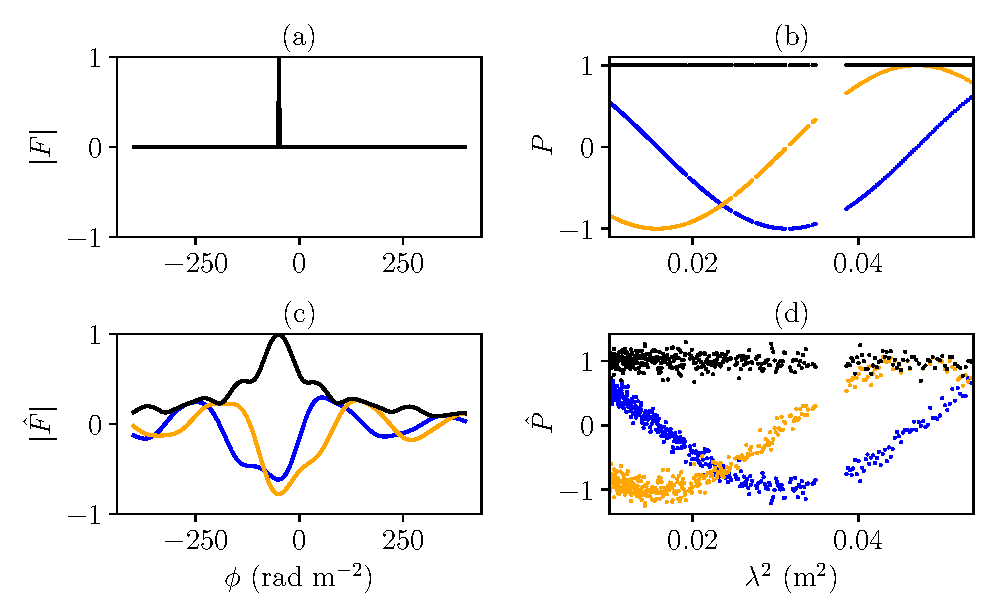
\includegraphics[width=0.9\linewidth]{faraday-images/spectra_simple.pdf}
      \caption[A simple FDF and its corresponding polarised spectra.]{A simple FDF and its corresponding polarised spectra: (a) groundtruth FDF $F$, (b) noise-free polarised spectrum $P$, (c) noisy observed FDF $\hat F$, (d) noisy polarised spectrum $\hat P$. Blue and orange mark real and imaginary components respectively.}
      \label{fig:faraday-simple-fdf}
    \end{figure}

    \begin{figure}
      \centering
      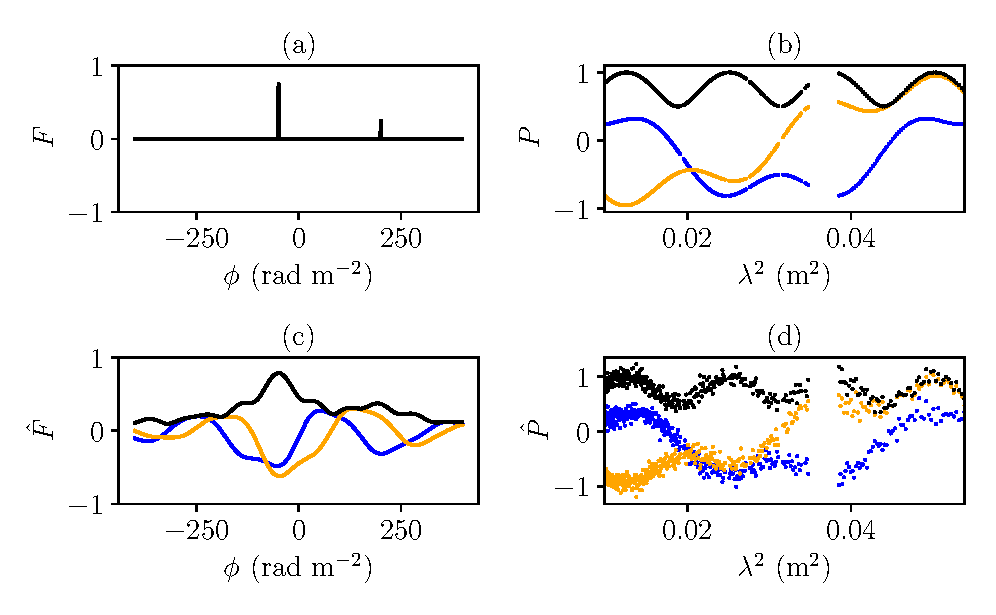
\includegraphics[width=0.94\linewidth]{faraday-images/spectra.pdf}
      \caption[A complex FDF and its corresponding polarised spectra.]{A complex FDF and its corresponding polarised spectra: (a) groundtruth FDF $F$, (b) noise-free polarised spectrum $P$, (c) noisy observed FDF $\hat F$, (d) noisy polarised spectrum $\hat P$. Blue and orange mark real and imaginary components respectively.}
      \label{fig:faraday-complex-fdf}
    \end{figure}

    Before we can classify FDFs as Faraday complex or Faraday simple, we need to define FDFs and any assumptions we make about them. An FDF is a function that maps Faraday depth $\phi$ to complex polarisation. It is the distribution of Faraday depths in an observed polarisation spectrum. For a given observation, we assume \DIFaddbegin \DIFadd{that }\DIFaddend there is a true, noise-free FDF $F$ composed of at most two Faraday screens. This accounts for most actual sources \citep{anderson_broadband_2015} and extension to three screens would cover most of the remainder---\citet{osullivan_broad-band_2017} found that 89 per cent of their sources were best explained by two or \DIFdelbegin \DIFdel{less }\DIFdelend \DIFaddbegin \DIFadd{fewer }\DIFaddend screens, while the remainder were best explained by three screens. We model the screens by Dirac delta distributions:
    \begin{equation}
        \label{eq:faraday-true-fdf}
        F(\phi) = A_0 \delta(\phi - \phi_0) + A_1 \delta(\phi - \phi_1).
    \end{equation}
    $A_0$ and $A_1$ are the polarised flux of each Faraday screen, and $\phi_0$ and $\phi_1$ are the Faraday depths of the respective screens. With this model, a Faraday simple source is one which has $A_0 = 0$, $A_1 = 0$, or $\phi_0 = \phi_1$. By using delta distributions to model each screen, we are assuming that there is no internal Faraday dispersion (which is typically associated with diffuse emission rather than the \DIFdelbegin \DIFdel{mostly-compact }\DIFdelend \DIFaddbegin \DIFadd{mostly compact }\DIFaddend sources we expect to find in wide-area polarised surveys). $F$ generates a polarised spectrum of the form shown in \autoref{eq:faraday-true-pol}:
    \begin{equation}
        \label{eq:faraday-true-pol}
        P(\lambda^2) = A_0 e^{2i\phi_0\lambda^2} + A_1 e^{2i\phi_1\lambda^2}.
    \end{equation}
    Such a spectrum would be observed as noisy samples from a number of squared wavelengths $\lambda^2_j, j \in [1, \dots, D]$. We model this noise as a complex Gaussian with standard deviation $\sigma$ and call the noisy observed spectrum $\hat P$:
    \begin{equation}
      \label{eq:faraday-noisy-pol}
      \hat P(\lambda_j^2) \sim \mathcal N(P(\lambda^2_j), \sigma^2).
    \end{equation}
    The constant variance of the noise is a simplifying assumption which may not hold for real data, and exploring this is a topic for future work. By performing RM synthesis \citep{brentjens_faraday_2005} on $\hat P$ with uniform weighting we arrive at an observed FDF:
    \begin{equation}
      \label{eq:faraday-rm-synthesis}
      \hat F(\phi) = \frac{1}{D} \sum_{j = 1}^D \hat P(\lambda^2_j) e^{-2i\phi\lambda^2_j}.
    \end{equation}
    Examples of $F$, $\hat F$, $P$, and $\hat P$ for simple and complex observations are shown in \autoref{fig:faraday-simple-fdf} and \autoref{fig:faraday-complex-fdf} respectively. Note that there are two reasons that the observed FDF $\hat F$ does not match the groundtruth FDF $F$. The first is the noise in $\hat P$. The second arises from the incomplete sampling of $\hat P$.

    We do not consider external or internal Faraday dispersion in this work. External Faraday dispersion would broaden the delta functions of \autoref{eq:faraday-true-fdf} into peaks, and internal Faraday dispersion would broaden them into top-hat functions. All sources have at least a small amount of dispersion as the Faraday depth is a bulk property of the intervening medium and is subject to noise, but the assumption we make is that this dispersion is sufficiently small that the groundtruth FDFs are well-modelled with delta functions. Faraday thick sources would also invalidate our assumptions, and we assume that there are none in our data as Faraday thickness can be consistent with a two-component model depending on the wavelength sampling \citep[e.g.][]{ma_broad-band_2019,brentjens_faraday_2005}. Nevertheless some external Faraday dispersion \DIFdelbegin \DIFdel{would be }\DIFdelend \DIFaddbegin \DIFadd{is }\DIFaddend covered by our model, as depending on observing parameters Faraday thick sources may appear as two screens \citep{van_eck_faraday_2017}.

    To simulate observed FDFs we follow the method of \citet{brown_classifying_2018}, which we describe in \DIFdelbegin %DIFDELCMD < \autoref{sec:faraday-simulating}%%%
\DIFdelend \DIFaddbegin \aref{sec:faraday-simulating}\DIFaddend .

\section{Classification approach}
\label{sec:faraday-approach}

  The Faraday complexity classification problem is as follows: Given an FDF $\hat F$, is it Faraday complex or Faraday simple? In this section we describe the features that we have developed to address this problem, which can be used in any standard machine learning classifier. We trained two classifiers on these features, which we describe here also.

  \subsection{Features}
  \label{sec:faraday-scores-method}

    Our features are based on a simple idea: \DIFdelbegin \DIFdel{all }\DIFdelend \DIFaddbegin \DIFadd{All }\DIFaddend simple FDFs look essentially the same, up to scaling and translation, while complex FDFs may deviate. A noise-free peak-normalised simple FDF $\hat F_{\mathrm{simple}}$ has the form\DIFaddbegin \DIFadd{:
    }\DIFaddend \begin{align}
        \label{eq:faraday-f-simple}
        \hat F_{\mathrm{simple}}(\phi; \phi_s) &= R(\phi - \phi_s).
    \end{align}
    where $R$ is the rotation measure spread function (RMSF), the Fourier transform of the wavelength sampling function which is 1 at all observed wavelengths and 0 otherwise. $\phi_s$ traces out a curve in the space of all possible FDFs. In other words, $\hat F_{\mathrm{simple}}$ is a manifold parametrised by $\phi_s$. Our features are derived from relating an observed FDF to the manifold of simple FDFs (the `simple manifold'). We measure the distance of an observed FDF to the simple manifold using distance measure $D_f$, that \DIFdelbegin \DIFdel{take }\DIFdelend \DIFaddbegin \DIFadd{takes }\DIFaddend all values of the FDF into account:
    \begin{equation}
        \label{eq:faraday-complexity-model}
        \varsigma_f(\hat F) = \min_{\phi_s \in \mathbb{R}} D_f\infdivx{\hat F(\phi)}{\hat F_{\mathrm{simple}}(\phi; \phi_s)}.
    \end{equation}
    We propose two distances that have nice properties:
    \begin{itemize}
        \item invariant over changes in complex phase,
        \item translationally invariant in Faraday depth,
        \item zero for Faraday simple sources (i.e. when $A_0 = 0$, $A_1 = 0$, or $\phi_0 = \phi_1$) when there is no noise,
        \item symmetric in components (i.e. swapping $A_0 \leftrightarrow A_1$ and $\phi_0 \leftrightarrow \phi_1$ should not change the distance),
        \item increasing as $A_0$ and $A_1$ become closer to each other, and
        \item increasing as screen separation $|\phi_0 - \phi_1|$ increases over a large range.
    \end{itemize}
    Our features are constructed from this distance and its minimiser. In other words
    we look for the simple FDF $\hat{F}_{\mathrm{simple}}$ that is \DIFdelbegin \DIFdel{``closest'' }\DIFdelend \DIFaddbegin \DIFadd{`closest' }\DIFaddend to the observed FDF $\hat{F}$.
    The minimiser $\phi_s$ is the Faraday depth of the simple FDF.

    While we could choose any distance that operates on functions, we used the 2-Wasserstein ($W_2$) distance (\autoref{eq:faraday-W2-distance}) and the Euclidean distance (\autoref{eq:faraday-Euclidean-distance}). The $W_2$ distance operates on probability distributions and can be thought of as the minimum cost to `move' one probability distribution to the other, where the cost of moving one unit of probability mass is the squared distance it is moved. Under $W_2$ distance, the minimiser $\phi_w$ in \autoref{eq:faraday-complexity-model} can be interpreted as the Faraday depth that the FDF $\hat F$ would be observed to have if its complexity was unresolved (i.e. the weighted mean of its components). The Euclidean distance is the square root of the least-squares loss which is often used for fitting $\hat{F}_{\mathrm{simple}}$ to the FDF $\hat F$. Under Euclidean distance, the minimiser $\phi_s$ is equivalent to the depth of the best-fitting single component under assumption of Gaussian noise in $\hat F$.
    We calculated the $W_2$ distance using \texttt{Python Optimal Transport} \citep{flamary17pot}, and we calculated the Euclidean distance using \texttt{scipy.spatial.distance.euclidean} \citep{virtanen20scipy}.
    Further intuition about the two distances is provided in \autoref{sec:faraday-interpreting-distances}.

    We denote by $\phi_w$ and $\phi_e$, the Faraday depth of the simple FDF that minimises the respective distances
    (2-Wasserstein and Euclidean).
    \begin{align*}
       \phi_w &= \underset{\phi_w}{\mathrm{argmin}}\ D_{W_2}\infdivx{\hat F(\phi)}{\hat F_{\mathrm{simple}}(\phi; \phi_w)},\\
       \phi_e &= \underset{\phi_e}{\mathrm{argmin}}\ D_E\infdivx{\hat F(\phi)}{\hat F_{\mathrm{simple}}(\phi; \phi_e)}.
     \end{align*}
     These features are depicted on an example FDF in \autoref{fig:faraday-features-on-fdf}.
     For simple observed FDFs, the fitted Faraday depths $\phi_w$ and $\phi_e$ both tend to be
     close to the peak of the observed FDF. However for complex observed FDFs, $\phi_w$ tends
     to be at the average depth between the two major peaks of the observed FDF, being closer
     to the higher peak. For notation convenience, we denote the Faraday depth of the
     observed FDF that has largest magnitude as $\phi_a$, i.e.
     \begin{equation*}
       \phi_a = \underset{\phi_a}{\mathrm{argmax}}\ |\hat F(\phi_a)|\DIFdelbegin \DIFdel{,}%DIFDELCMD < \\
%DIFDELCMD <      %%%
\DIFdelend \DIFaddbegin \DIFadd{.
     }\DIFaddend \end{equation*}
     Note that in practice $\phi_a \approx \phi_e$.
     For complex observed FDFs, the values of Faraday depths $\phi_w$ and $\phi_a$ tend
     to differ (essentially by a proportion of the location of the second screen).
     The difference between $\phi_w$ and $\phi_a$ therefore provides useful information
     to identify complex FDFs.
     When the observed FDF is simple, the 2-Wasserstein fit \DIFdelbegin \DIFdel{will overlap }\DIFdelend \DIFaddbegin \DIFadd{overlaps }\DIFaddend significantly,
     hence the observed magnitudes $\hat F(\phi_w)$ and $\hat F(\phi_a)$ will be similar.
     However, for complex FDFs\DIFaddbegin \DIFadd{, }\DIFaddend $\phi_w$ and $\phi_a$ are at different depths,
     leading to different values of $\hat F(\phi_w)$ and $\hat F(\phi_a)$.
     Therefore the magnitudes of the observed FDFs at the depths $\phi_w$ and $\phi_a$
     indicate how different the observed FDF is from a simple FDF.

    \begin{figure}
      \centering
      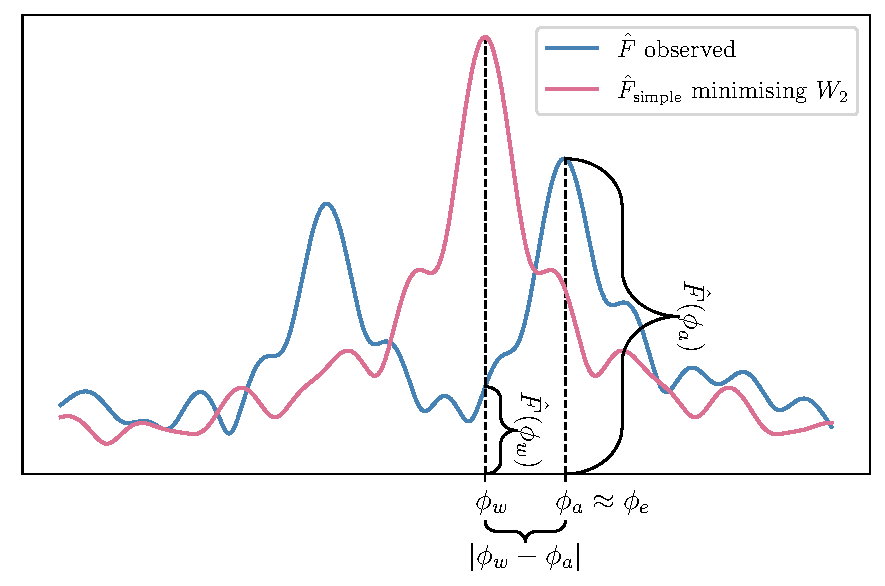
\includegraphics[width=0.7\linewidth]{faraday-images/features_on_graph.pdf}
      \caption[An illustration of our FDF features.]{\label{fig:faraday-features-on-fdf} An example of how an observed FDF $\hat F$ relates to our features. $\phi_w$ is the $W_2$-minimising Faraday depth, and $\phi_a$ is the $\hat F$-maximising Faraday depth (approximately equal to the Euclidean-minimising Faraday depth). The remaining two features are the $W_2$ and Euclidean distances between the depicted FDFs.}
    \end{figure}

    In summary, we provide the following features to the classifier:
    \begin{itemize}
      \item $\log |\phi_w - \phi_a|$,
      \item $\log \hat F(\phi_w)$,
      \item $\log \hat F(\phi_a)$,
      \item $\log D_{W_2}\infdivx{\hat F(\phi)}{\hat F_{\mathrm{simple}}(\phi; \phi_w)}$,
      \item $\log D_{E}\infdivx{\hat F(\phi)}{\hat F_{\mathrm{simple}}(\phi; \phi_e)}$,
    \end{itemize}
    where $D_E$ is the Euclidean distance, $D_{W_2}$ is the $W_2$ distance, $\phi_a$ is the Faraday depth of the FDF peak, $\phi_w$ is the minimiser for $W_2$ distance, and $\phi_e$ is the minimiser for Euclidean distance.

    \subsection{Interpreting distances}
    \label{sec:faraday-interpreting-distances}

    Interestingly, in the case where there is no RMSF, \autoref{eq:faraday-complexity-model} with $W_2$ distance reduces to the Faraday moment already in common use:
    \begin{align}
        D_{W_2}(F) &= \min_{\phi_w \in \mathbb{R}} D_{W_2}\infdivx{F(\phi)}{F_{\mathrm{simple}}(\phi; \phi_w)}\label{eq:faraday-W2-distance}\\
            &= \left(\frac{A_0A_1}{(A_0 + A_1)^2} (\phi_0 - \phi_1)^2\right)^{1/2}.
    \end{align}
    See \DIFdelbegin %DIFDELCMD < \autoref{sec:faraday-w2-to-faraday-moments} %%%
\DIFdelend \DIFaddbegin \aref{sec:faraday-w2-to-faraday-moments} \DIFaddend for the corresponding calculation. In this sense, the $W_2$ distance can be thought of as a generalised Faraday moment, and conversely an interpretation of Faraday moments as a distance from the simple manifold in the case where there is no RMSF. Euclidean distance behaves quite differently in this case, and the resulting distance measure is totally independent of Faraday depth:
    \begin{align}
        D_{E}(F) &= \min_{\phi_e \in \mathbb{R}} D_E\infdivx{F(\phi)}{F_{\mathrm{simple}}(\phi; \phi_e)}\label{eq:faraday-Euclidean-distance}\\
            &= \sqrt{2} \frac{\min(A_0, A_1)}{A_0 + A_1}.
    \end{align}
    See \aref{sec:faraday-euclidean-calculation} for the corresponding calculation.


  \subsection{Classifiers}
  \label{sec:faraday-classifiers}

    We trained two classifiers on simulated observations using these features: logistic regression (LR) and extreme gradient boosted trees (XGB). These classifiers are useful together for understanding Faraday complexity classification. LR is a linear classifier that is readily interpretable by examining the weights it applies to each feature, and is one of the simplest possible classifiers. XGB is a powerful off-the-shelf non-linear ensemble classifier, and is an example of a decision tree ensemble which are widely used in astronomy \citep[e.g.][]{machado_poletti_valle_shaping_2020,hlozek20lsst}. We used the \texttt{scikit-learn} implementation of LR and we \DIFdelbegin \DIFdel{use }\DIFdelend \DIFaddbegin \DIFadd{used }\DIFaddend the \texttt{XGBoost} library for XGB. We optimised hyperparameters for XGB using a fork of \texttt{xgboost-tuner}\footnote{\url{https://github.com/chengsoonong/xgboost-tuner}} as utilised by \citet{zhu20mutagenic}. We used \DIFdelbegin \DIFdel{1~000 }\DIFdelend \DIFaddbegin \DIFadd{1000 }\DIFaddend iterations of randomised parameter tuning and the hyperparameters we found are tabulated in \autoref{tab:faraday-hyperparameters-xgb}. We optimised hyperparameters for LR using a 5-fold cross-validation grid search implemented in \texttt{sklearn.model\textunderscore{}selection.GridSearchCV}. The resulting hyperparameters are tabulated in \autoref{tab:faraday-hyperparameters-lr} in \DIFdelbegin \DIFdel{the Appendix}\DIFdelend \DIFaddbegin \aref{sec:faraday-hyperparameters}\DIFaddend .

\section{Experimental method and results}
\label{sec:faraday-experiment-classification}

  We applied our classifiers to classify simulated (\autoref{sec:faraday-cnn-comparison} and \ref{sec:faraday-results-simulated}) and real (\autoref{sec:faraday-results-observed}) FDFs. We replicated the experimental setup of \citet{brown_classifying_2018} for comparison with the state-of-the-art CNN classification method, and we also applied our method to 142 real FDFs observed with the Australia Telescope Compact Array (ATCA) from \citet{livingston21faraday} and \citet{osullivan_broad-band_2017}.

  \subsection{Data}

  \subsubsection{Simulated training and validation data}
  \label{sec:faraday-simulated-training-data}

    Our classifiers were trained and validated on simulated FDFs. We produced two sets of simulated FDFs, one for comparison with the state-of-the-art method in the literature and one for application to our observed FDFs (described in \autoref{sec:faraday-observational-data}). We refer to the former as the `ASKAP' dataset as it uses frequencies from the Australian Square Kilometre Array Pathfinder 12-antenna early science configuration. These frequencies \DIFdelbegin \DIFdel{included }\DIFdelend \DIFaddbegin \DIFadd{include }\DIFaddend 900 channels from 700--1300 and 1500--1800~MHz and were used to generate simulated training and validation data by \citet{brown_classifying_2018}. We refer to the latter as the `ATCA' dataset as it uses frequencies from the 1--3~GHz configuration of the ATCA. These frequencies \DIFdelbegin \DIFdel{included }\DIFdelend \DIFaddbegin \DIFadd{include }\DIFaddend 394 channels from 1.29--3.02~GHz and match our real data. We simulated Faraday depths from $-50$ to $50$ rad~m$^{-2}$ for the `ASKAP' dataset (matching Brown) and $-500$ to $500$ \DIFaddbegin \DIFadd{rad~m$^{-2}$ }\DIFaddend for the `ATCA' dataset.

    For each dataset, we simulated 100~000 FDFs, approximately half simple and half complex. We randomly allocated half of these FDFs to a training set and reserved the remaining half for validation. Each FDF had complex Gaussian noise added to the corresponding polarisation spectrum. For the `ASKAP' dataset, we sampled the standard deviation of the noise uniformly between 0 and $\sigma_{\max} = 0.333$, matching the dataset of \citet{brown_classifying_2018}.
    For the `ATCA' dataset, we fit a log-normal distribution to the standard deviations of O'Sullivan's data \citep{osullivan_broad-band_2017} from which we sampled our values of $\sigma$:
    \begin{equation}
      \sigma \sim \frac{1}{0.63 \sqrt{2 \pi} \sigma} \exp \left(-\frac{\log\left(50 \sigma - 0.5\right)^2}{2 \times 0.63^2}\right)
    \end{equation}


  \subsubsection{Observational data}
  \label{sec:faraday-observational-data}

    We used two real datasets containing a total of 142 sources: 42 polarised spectra from Livingston et al. (2020, submitted) and 100 polarised spectra from \citet{osullivan_broad-band_2017}. These datasets were observed in similar frequency ranges on the same telescope (with different binning), but are in different parts of the sky. The Livingston data were taken near the Galactic Centre, and the O'Sullivan data were taken away from the plane of the Galaxy. There are more Faraday complex sources near the Galactic Centre compared to more Faraday simple sources away from the plane of the Galaxy (Livingston et al.). The similar frequency channels used in the two datasets result in almost identical RMSFs over the Faraday depth range we considered (-500 to 500 rad m$^{-2}$), so we expected that the classifiers would work equally well on both datasets with no need to re-train. We discarded the 26 Livingston sources with modelled Faraday depths outside of this Faraday depth range, which we do not expect to affect the applicability of our methods to wide-area surveys because these fairly high depths are not common.

    \citet{livingston21faraday} used \texttt{RM-CLEAN} \citep{heald09faraday} to identify significant components in their FDFs. Some of these components had very high Faraday depths up to 2000 rad m$^{-2}$, but we chose to ignore these components in this \DIFdelbegin \DIFdel{paper }\DIFdelend \DIFaddbegin \DIFadd{chapter }\DIFaddend as they are much larger than might be expected in a wide-area survey like POSSUM. They used the second Faraday moment \citep{brown11report} to estimate Faraday complexity, with Faraday depths determined using \texttt{scipy.signal.find\textunderscore{}peaks} on the cleaned FDFs, with a cutoff of \DIFdelbegin \DIFdel{7 }\DIFdelend \DIFaddbegin \DIFadd{seven }\DIFaddend times the noise of the polarised spectrum. Using this method, they estimated that 89 per cent of their sources were Faraday complex i.e. had a Faraday moment greater than \DIFdelbegin \DIFdel{0.
}\DIFdelend \DIFaddbegin \DIFadd{zero.
}\DIFaddend 

    \citet{osullivan_broad-band_2017} used the QU-fitting and model selection technique described in \citet{osullivan12agn}. The QU-fitting models contained up to three Faraday screen components as well as a term for internal and external Faraday dispersion. We ignore the Faraday thickness and dispersion for the purposes of this \DIFdelbegin \DIFdel{paper}\DIFdelend \DIFaddbegin \DIFadd{chapter}\DIFaddend , as most sources were not found to have Faraday thickness and dispersion is beyond the scope of our current work. 37 sources had just one component, 52 had two, and the remaining 11 had three.

  \subsection{Results on `ASKAP' dataset}
  \label{sec:faraday-cnn-comparison}

    \begin{table}[htbp]
      \caption{\label{tab:faraday-cms} Confusion matrix entries for LR and XGB on `ASKAP' and `ATCA' simulated datasets, and the CNN confusion matrix entries adapted from \citet{brown_classifying_2018}.}
      \centering
      \begin{tabular}{r|ccc|cc}
        \hline\hline
        & \multicolumn{3}{c}{`ASKAP'} & \multicolumn{2}{c}{`ATCA'} \\
        & LR & XGB & CNN & LR & XGB \\
        \hline
        True negative rate & 0.99 & 0.99 & 0.97 & 0.92 & 0.91\\
        False positive rate & 0.01 & 0.01 & 0.03 & 0.08 & 0.09\\
        False negative rate & 0.10 & 0.09 & 0.07 & 0.16 & 0.10\\
        True positive rate & 0.90 & 0.91 & 0.93 & 0.84 & 0.90\\
        \hline\hline
      \end{tabular}\\
    \end{table}

    The \DIFdelbegin \DIFdel{accuracy }\DIFdelend \DIFaddbegin \DIFadd{accuracies }\DIFaddend of the LR and XGB classifiers on the `ASKAP' testing set \DIFdelbegin \DIFdel{was }\DIFdelend \DIFaddbegin \DIFadd{were }\DIFaddend 94.4 and 95.1 per cent respectively. The rates of true and false identifications are summarised in \autoref{tab:faraday-cms}. These results are very close to the CNN presented by \citet{brown_classifying_2018}, with a slightly higher true negative rate and a slightly lower true positive rate (recalling that positive sources are complex, and negative sources are simple). The accuracy of the CNN was 94.9 \DIFaddbegin \DIFadd{per cent}\DIFaddend , slightly lower than our XGB classifier and slightly higher than our LR classifier. Both of our classifiers therefore \DIFdelbegin \DIFdel{produce }\DIFdelend \DIFaddbegin \DIFadd{produced }\DIFaddend similar classification performance to the CNN, with faster training time and easier interpretation.

  \subsection{Results on `ATCA' dataset}
  \label{sec:faraday-results-simulated}

    The \DIFdelbegin \DIFdel{accuracy }\DIFdelend \DIFaddbegin \DIFadd{accuracies }\DIFaddend of the LR and XGB classifiers on the `ATCA' dataset \DIFdelbegin \DIFdel{was }\DIFdelend \DIFaddbegin \DIFadd{were }\DIFaddend 89.2 and 90.5 per cent respectively. The major differences between the `ATCA' and the `ASKAP' experiments are the range of the simulated Faraday depths and the distribution of noise levels. The `ASKAP' dataset, to match past CNN work, only included depths from $-50$ to $50$ rad m$^{-2}$, while the `ATCA' dataset includes depths from $-500$ to $500$ rad m$^{-2}$. The rates of true and false identifications are again shown in \autoref{tab:faraday-cms}.

    \begin{figure}
      \begin{subfigure}{\linewidth}
        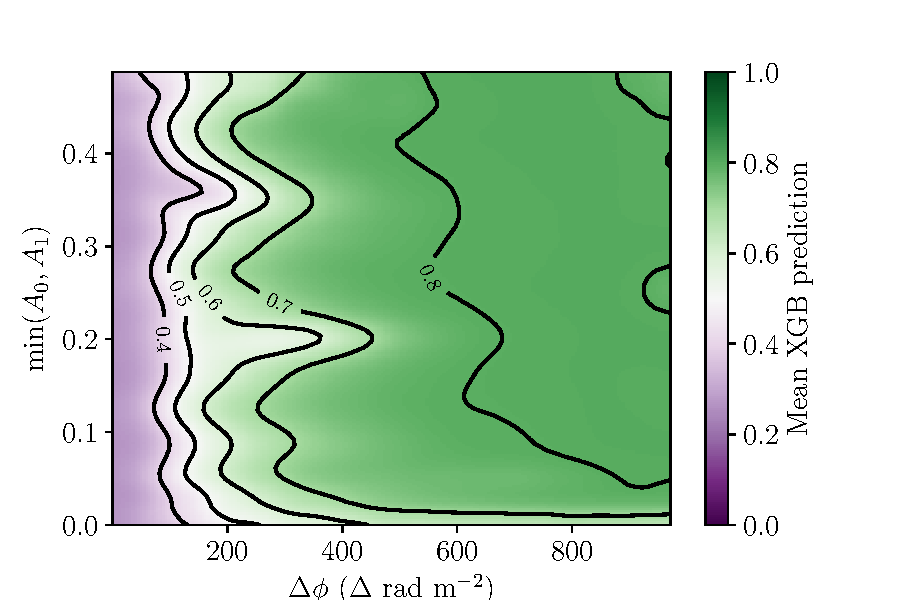
\includegraphics[width=\linewidth]{faraday-images/mean_xgb_prediction_dphi_amp.pdf}
        \caption{\label{fig:faraday-mean-xgb-pred}}
      \end{subfigure}
      \begin{subfigure}{\linewidth}
        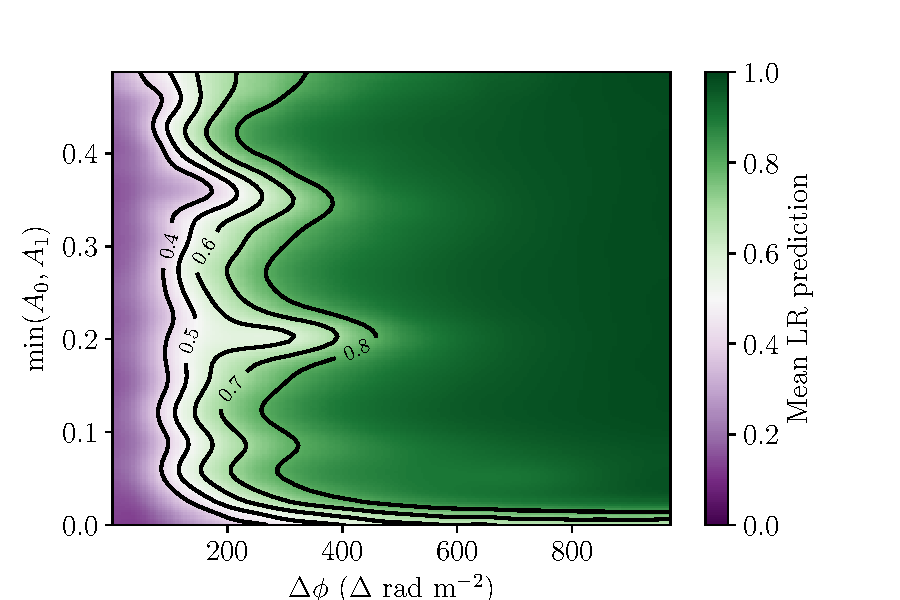
\includegraphics[width=\linewidth]{faraday-images/mean_lr_prediction_dphi_amp.pdf}
        \caption{\label{fig:faraday-mean-lr-pred}}
      \end{subfigure}
      \caption[Mean prediction as a function of component depth separation and minimum component amplitude for XGB and LR.]{\label{fig:faraday-amps-dphi-mean} Mean prediction as a function of component depth separation and minimum component amplitude for (a) XGB and (b) LR.}
    \end{figure}

    As we know the true Faraday depths of the components in our simulation, we can investigate the behaviour of these classifiers as a function of physical properties. \autoref{fig:faraday-amps-dphi-mean} shows the mean classifier prediction as a function of component depth separation and minimum component amplitude. This is tightly related to the mean accuracy, as the entire plot domain contains complex spectra besides the left and bottom edge: by thresholding the classifier prediction to a certain value, the accuracy will be one hundred per cent on the non-edge for all sources with higher prediction values.

  \subsection{Results on observed FDFs}
  \label{sec:faraday-results-observed}

    \begin{figure*}
      \centering
      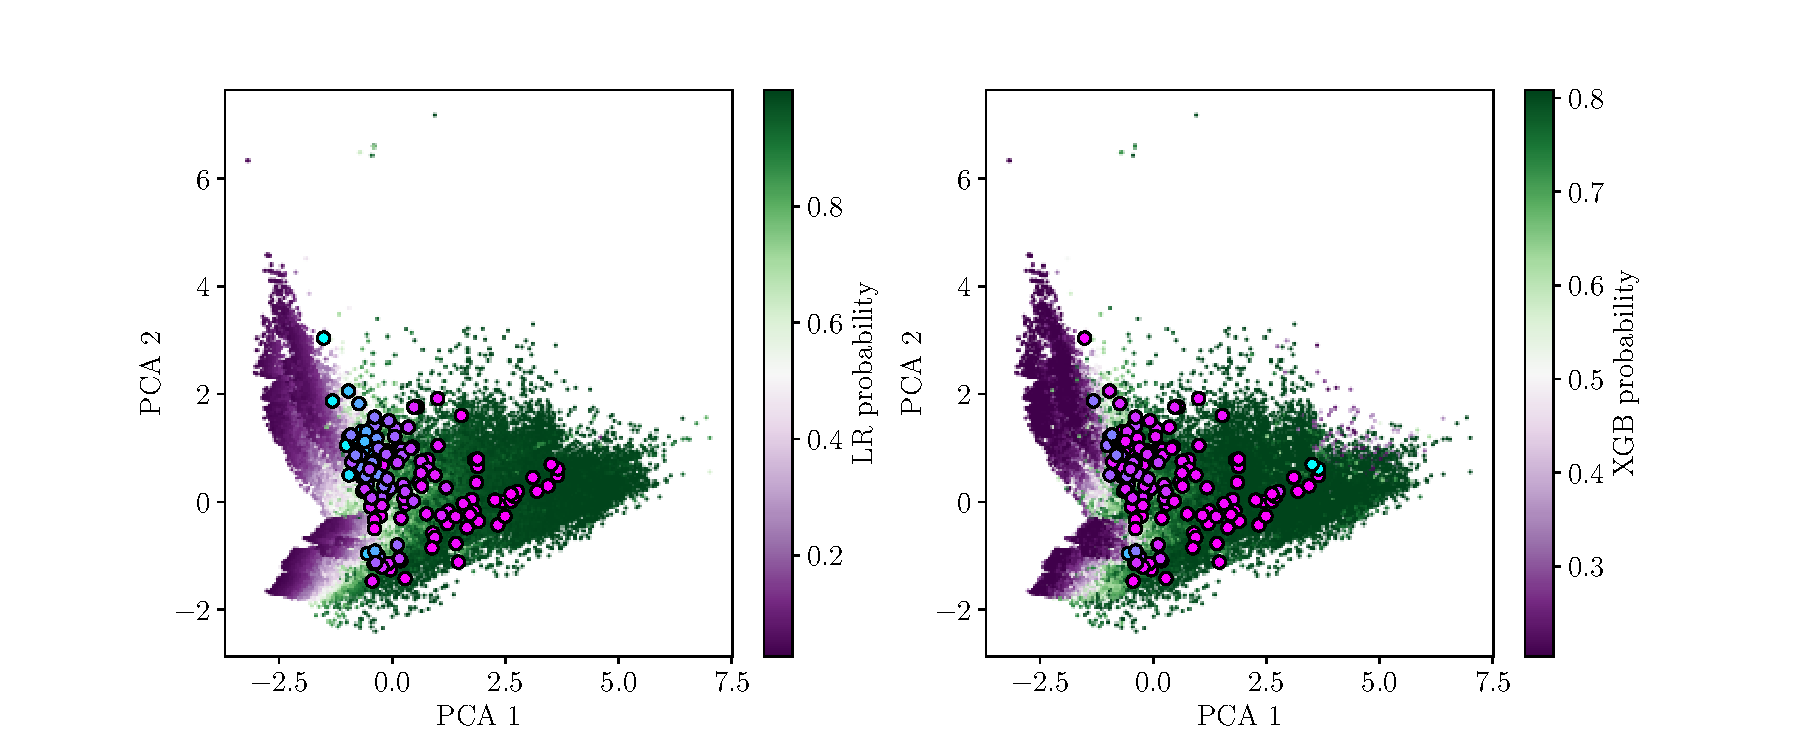
\includegraphics[width=\linewidth]{faraday-images/pca_with_overlay.pdf}
      \caption[Principal component analysis for simulated data with observations overlaid.]{Principal component analysis for simulated data (coloured dots) with observations overlaid (black-edged circles). Observations are coloured by their XGB or LR estimated probability of being complex, with blue indicating `most simple' and pink indicating `most complex'.}
      \label{fig:faraday-pca}
    \end{figure*}
    \begin{figure}
      \centering
      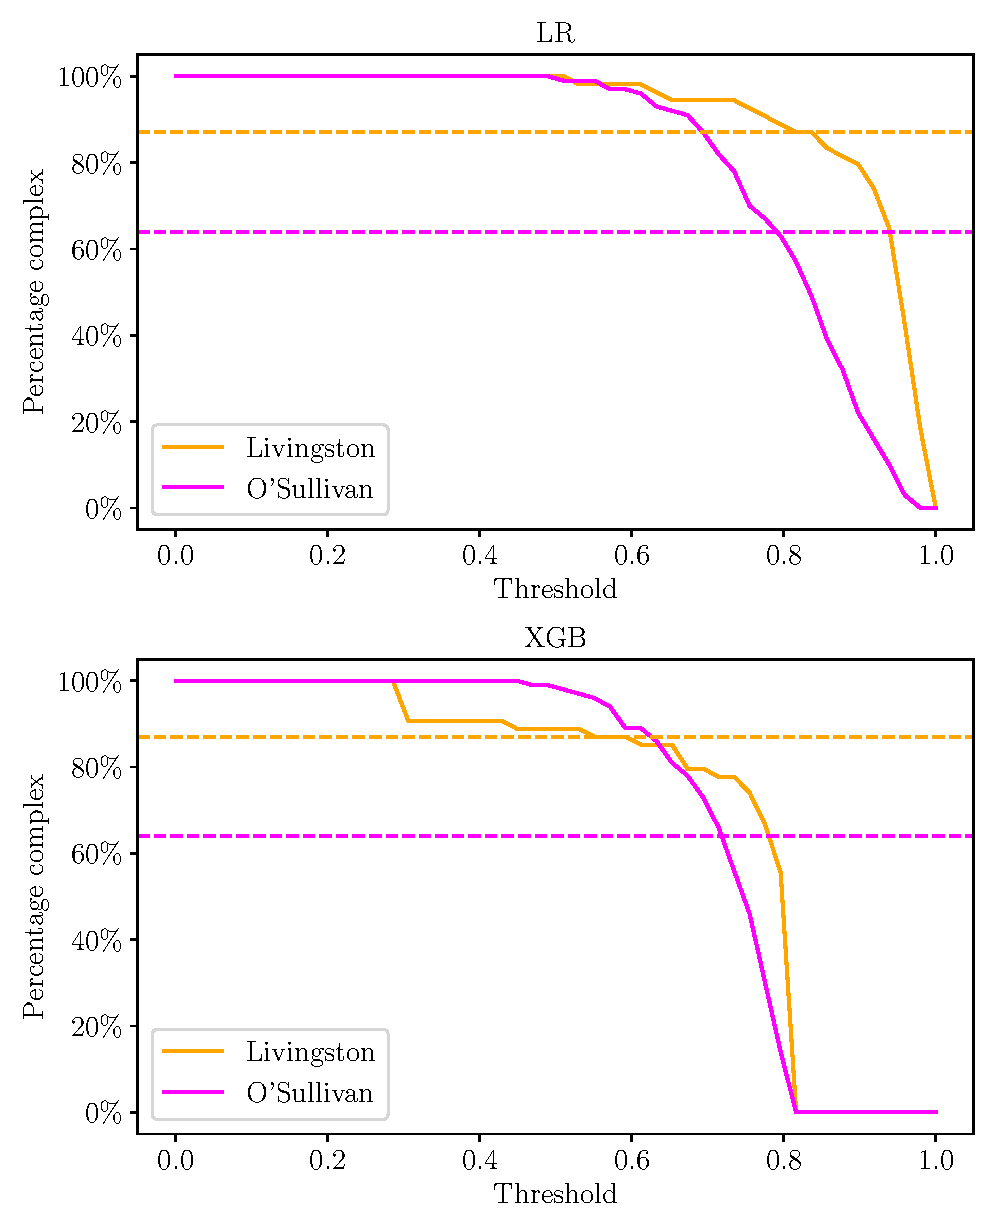
\includegraphics[width=\linewidth]{faraday-images/pc_complex_curves.pdf}
      \caption[Estimated rates of Faraday complexity for the Livingston and O'Sullivan datasets as functions of threshold.]{Estimated rates of Faraday complexity for the Livingston and O'Sullivan datasets as functions of threshold. The horizontal lines indicate the rates of Faraday complexity estimated by Livingston and O'Sullivan respectively.}
      \label{fig:faraday-complexity-rates}
    \end{figure}

    We used the LR and XGB classifiers which were trained on the `ATCA' dataset to estimate the probability that our 142 observed FDFs (\autoref{sec:faraday-observational-data}) were Faraday complex. As these classifiers were trained on simulated data, they face the issue of the `domain gap': \DIFdelbegin \DIFdel{the }\DIFdelend \DIFaddbegin \DIFadd{The }\DIFaddend distribution of samples from a simulation differs from the distribution of real sources, and this affects performance on real data. Solving this issue is called `domain adaptation' and how to do this is an open research question in machine learning \citep{zhang2019transfer,pan10transfer}. Nevertheless, the features of our observations mostly fall in the same region of feature space as the simulations (\autoref{fig:faraday-pca}) and so we expect reasonably good domain transfer.

    Two apparently complex sources in the Livingston sample are classified as simple with high probability by XGB. These outliers are on the very edge of the training sample (\autoref{fig:faraday-pca}) and the underdensity of training data here is likely the cause of this issue. LR does not suffer the same issue, producing plausible predictions for the entire dataset, and these sources are instead classified as complex with high probability.

    With a threshold of 0.5, LR predicted that 96 and 83 per cent of the Livingston and O'Sullivan sources were complex respectively. This is in line with expectations that the Livingston data should have more Faraday complex sources than the O'Sullivan data due to their location near the Galactic Centre. XGB predicted that 93 and 100 per cent of the Livingston and O'Sullivan sources were complex respectively. \citet{livingston21faraday} found that 90 per cent of their sources were complex, and \citet{osullivan_broad-band_2017} found that 64 per cent of their sources were complex. This suggests that our classifiers are overestimating complexity, though it could also be the case that the methods used by Livingston and O'Sullivan underestimate complexity. Modifying the prediction threshold from 0.5 changes the estimated rate of Faraday complexity, and we show the estimated rates against threshold for both classifiers in \autoref{fig:faraday-complexity-rates}. We suggest that this result is indicative of our probabilities being uncalibrated, and a higher threshold should be chosen in practice. We chose to keep the threshold at 0.5 as this had the highest accuracy on the simulated validation data. The very high complexity rates of XGB and two outlying classifications indicate that the XGB classifier may be overfitting to the simulation and that it is unable to generalise across the domain gap.

    \autoref{fig:faraday-all-observed-fdfs-lr} and \autoref{fig:faraday-all-observed-fdfs-xgb} \DIFaddbegin \DIFadd{in }\aref{sec:faraday-real-data-fig} \DIFaddend show every observed FDF ordered by estimated Faraday complexity, alongside the models predicted by Livingston and \citet{osullivan_broad-band_2017} \DIFdelbegin \DIFdel{, }\DIFdelend for LR and XGB respectively. There is a clear visual trend of increasingly complex sources with increasing predicted probability of being complex.

\section{Discussion}
\label{sec:faraday-discussion}

  On simulated data (\autoref{sec:faraday-results-simulated}) we achieve state-of-the-art accuracy. Our results on observed FDFs show that our classifiers produce plausible results, with \autoref{fig:faraday-all-observed-fdfs-lr} and \autoref{fig:faraday-all-observed-fdfs-xgb} showing a clear trend of apparent complexity. Some issues remain: \DIFdelbegin \DIFdel{we }\DIFdelend \DIFaddbegin \DIFadd{We }\DIFaddend discuss the intrinsic overlap between simple and complex FDFs in \autoref{sec:faraday-overlap} and the limitations of our method in \autoref{sec:faraday-limitations}.

  \subsection{Complexity and seeming `not simple'}
  \label{sec:faraday-overlap}

    Through this work we found our methods limited by the significant overlap between complex and simple FDFs. Complex FDFs can be consistent with simple FDFs due to close Faraday components or very small amplitudes on the secondary component, and vice versa due to noise.

    The main failure mode of our classifiers is misclassifying a complex source as simple (\autoref{tab:faraday-cms}). Whether sources with close components or small amplitudes should be considered complex is not clear, since for practical purposes they can be treated as simple: \DIFdelbegin \DIFdel{assuming }\DIFdelend \DIFaddbegin \DIFadd{Assuming }\DIFaddend the source is simple yields a very similar RM to the RM of the primary component, and thus would not negatively impact further data products such as an RM grid. The scenarios where we would want a Faraday complexity classifier rather than a polarisation structure model -- large-scale analysis and wide-area surveys -- do not seem to be disadvantaged by considering such sources simple. Additional sources similar to these are likely hidden in presumably `simple' FDFs by the frequency range and spacing of the observations, just as how these complex sources would be hidden in lower-resolution observations. Note also that misidentification of complex sources as simple is intrinsically a problem with complexity estimation even for models not well-represented by a simple FDF, as complex sources may conspire to appear as a wide range of viable models including simple \citep{sun15comparison}.

    Conversely, high-noise simple FDFs may be consistent with complex FDFs. One key question is how Faraday complexity estimators should behave as the noise increases: \DIFdelbegin \DIFdel{should }\DIFdelend \DIFaddbegin \DIFadd{Should }\DIFaddend high noise result in a complex prediction or a simple prediction, given that \DIFdelbegin \DIFdel{a complex or simple FDF would both }\DIFdelend \DIFaddbegin \DIFadd{both complex and simple FDFs would }\DIFaddend be consistent with a noisy FDF? Occam's razor suggests that we should choose the simplest suitable model, and so increasing noise should lead to predictions of less complexity. This is not how our classifiers operate, however: \DIFdelbegin \DIFdel{high-noise }\DIFdelend \DIFaddbegin \DIFadd{High-noise }\DIFaddend FDFs are different to the model simple FDFs and so are predicted to be `not simple'. In some sense our classifiers are not looking for complex sources, but are rather looking for `not simple' sources.

  \subsection{Limitations}
  \label{sec:faraday-limitations}

    Our main limitations are our simplifying assumptions on FDFs and the domain gap between simulated and real observations. However, our proposed features (Section~\autoref{sec:faraday-scores-method}) can be applied to future improved simulations.

    It is unclear what the effect of our simplifying assumptions are on the effectiveness of our simulation. The three main simplifications that may negatively affect our simulations are 1) limiting to two components, 2) assuming no external Faraday dispersion, and 3) assuming no internal Faraday dispersion (Faraday thickness). Future work will explore removing these simplifying assumptions, but will need to account for the increased difficulty in characterising the simulation with more components and no longer having Faraday screens as components. Additionally, more work will be required to make sure that the rates of internal and external Faraday dispersion match what might be expected from real sources, or risk making a simulation that has too large a range of consistent models for a given source: \DIFdelbegin \DIFdel{for }\DIFdelend \DIFaddbegin \DIFadd{For }\DIFaddend example, a two-component source could also be explained as a sufficiently wide or resolved-out Faraday thick source or a three-component source with a small third component. This greatly complicates the classification task.

    Previous machine learning work \citep[e.g.][]{brown_classifying_2018} has not been run before on real FDF data, so this \DIFdelbegin \DIFdel{paper }\DIFdelend \DIFaddbegin \DIFadd{chapter }\DIFaddend is the first example of the domain gap arising in Faraday complexity classification. This is a problem that requires further research to solve. We have no good way to ensure that our simulation matches reality, so some amount of domain adaptation will always be necessary to train classifiers on simulated data and then \DIFaddbegin \DIFadd{to }\DIFaddend apply these classifiers to real data. But with the low source counts in polarisation science (high-resolution spectropolarimetric data currently numbers in the few hundreds) any machine learning method will need to be trained on simulations. This is not just a problem in Faraday complexity estimation, and domain adaptation is also an issue faced in the wider astroinformatics community: \DIFdelbegin \DIFdel{large }\DIFdelend \DIFaddbegin \DIFadd{Large }\DIFaddend quantities of labelled data are hard to come by, and some sources are very rare \citep[e.g. gravitational wave detections or fast radio bursts;][]{zevin17gravityspy, gebhard19convolutional,agarwal_fetch_2020}. LR seems to handle the domain adaptation better than XGB, with only a slightly lower accuracy on simulated data. Our results are plausible and the distribution of our simulation well overlaps the distribution of our real data (\autoref{fig:faraday-pca}).

\section{Conclusion}
\label{sec:faraday-conclusion}

  We developed a simple, interpretable machine learning method for estimating Faraday complexity. Our interpretable features were derived by comparing observed FDFs to idealised simple FDFs, which we could determine \DIFdelbegin \DIFdel{both for }\DIFdelend \DIFaddbegin \DIFadd{for both }\DIFaddend simulated and real observations. We demonstrated the effectiveness of our method on both simulated and real data. Using simulated data, we found that our classifiers were 95 per cent accurate, with near perfect recall (specificity) of Faraday simple sources. On simulated data that matched existing observations, our classifiers obtained an accuracy of 90 per cent. Evaluating our classifiers on real data gave the plausible results shown in \autoref{fig:faraday-all-observed-fdfs-lr}, and marks the first application of machine learning to observed FDFs. Future work will need to narrow the domain gap to improve transfer of classifiers trained on simulations to real, observed data.

\section{Acknowledgements}

This research was conducted in Canberra, on land for which the Ngunnawal and Ngambri people are the traditional and ongoing custodians. M.J.A. and J.D.L. were supported by the Australian Government Research Training Program. M.J.A. was supported by the Astronomical Society of Australia. The Australia Telescope Compact Array is part of the Australia Telescope National Facility which is funded by the Australian Government for operation as a National Facility managed by CSIRO. We acknowledge the Gomeroi people as the traditional \DIFdelbegin \DIFdel{owners }\DIFdelend \DIFaddbegin \DIFadd{custodians }\DIFaddend of the Observatory site. We thank the anonymous referee for their comments on this work.
\DIFaddbegin 


\appendix

\section{\DIFadd{Simulating observed FDFs}}
\label{sec:faraday-simulating}

  \DIFadd{This appendix describes how we simulated FDFs in }\autoref{cha:faraday}\DIFadd{. We simulate FDFs by approximating them by arrays of complex numbers. An FDF $F$ is approximated on the domain $[-\phi_{\max}, \phi_{\max}]$ by a vector $\vec F \in \mathbb R^d$:
    }\begin{equation}
      \DIFadd{\label{eq:faraday-vec-f}
      \vec F_j = \sum_{k = 0}^1 A_k \delta(-\phi_{\max} + j \delta \phi - \phi_k)
    }\end{equation}
    \DIFadd{where $\delta\phi = (\phi_{\max} - \phi_{\min}) / d$ and $d$ is the number of Faraday depth samples in the FDF.
    $\vec F$ is sampled by uniformly sampling its parameters:
    }\begin{align}
      \DIFadd{\label{eq:faraday-model-distributions}
      \phi_k }&\DIFadd{\in }[\DIFadd{\phi_{\min}, \phi_{\min} + \delta\phi, \dots, \phi_{\max}}]\\
      \DIFadd{A_k }&\DIFadd{\sim \mathcal U(0, 1).
    }\end{align}
    \DIFadd{We then generate a vector polarisation spectrum $\vec P \in \mathbb R^m$ from $\vec F$ using a }\autoref{eq:faraday-discrete-f-to-p}\DIFadd{:
    }\begin{equation}
      \DIFadd{\label{eq:faraday-discrete-f-to-p}
      \vec P_\ell = \sum_{j = 0}^{j} F_j e^{2i(\phi_{\min} + j\delta_\phi)\lambda^2_\ell}\ \mathrm{d}\phi.
    }\end{equation}
    \DIFadd{$\lambda^2_\ell$ is the discretised value of $\lambda^2$ at the $\ell$th index of $\vec P$. This requires a set of $\lambda^2$ values, which depends on the dataset being simulated. These values can be treated as the channel wavelengths at which the polarisation spectrum was observed. We then add Gaussian noise with variance $\sigma^2$ to each element of $\vec P$ to obtain a discretised noisy observation $\hat{\vec{P}}$. Finally, we perform RM synthesis using the Canadian Initiative for Radio Astronomy Data Analysis }\texttt{\DIFadd{RM}} \DIFadd{package}\footnote{\url{https://github.com/CIRADA-Tools/RM}}\DIFadd{, which is a }\texttt{\DIFadd{Python}} \DIFadd{module that implements a discrete version of RM synthesis:
    }\begin{equation}
      \DIFadd{\label{eq:faraday-discrete-rm-synthesis}
      \hat{\vec{F}}_j = m^{-1} \sum_{\ell = 1}^m \vec{\hat P}_\ell e^{-2i(\phi_{\min} + j\delta_\phi)\lambda^2_\ell}.
    }\end{equation}

\section{\DIFadd{2-Wasserstein begets Faraday moments}}
  \label{sec:faraday-w2-to-faraday-moments}
    \DIFadd{Minimising the 2-Wasserstein distance between a model FDF and the simple manifold gives the second Faraday moment of that FDF. This appendix demonstrates that fact. Let $\tilde F$ be the sum-normalised model FDF and let $\tilde S$ be the sum-normalised simple model FDF:
    }\begin{align}
      \DIFadd{\tilde F(\phi) }&\DIFadd{= \frac{A_0 \delta(\phi - \phi_0) + A_1 \delta(\phi - \phi_1)}{A_0 + A_1}}\\
      \DIFadd{\tilde S(\phi; \phi_w) }&\DIFadd{= \delta(\phi - \phi_w).
    }\end{align}
    \DIFadd{The $W_2$ distance, usually defined on probability distributions, can be extended to one-dimensional complex functions $A$ and $B$ by normalising them:
      }\begin{align}
        \DIFadd{\label{eq:faraday-w2}
        D_{W_2}\infdivx{A}{B}^2 }&\DIFadd{= \inf_{\gamma \in \Gamma(A, B)} \iint_{\phi_{\min}}^{\phi_{\max}} |x - y|^2\ \mathrm{d}\gamma(x, y) }\\
        \DIFadd{\label{eq:faraday-normalised}
        \tilde A(\phi) }&\DIFadd{= \frac{|A(\phi)|}{\int_{\phi_{\min}}^{\phi_{\max}} |A(\theta)|\ \mathrm{d}\theta}}\\
        \DIFadd{\tilde B(\phi) }&\DIFadd{= \frac{|B(\phi)|}{\int_{\phi_{\min}}^{\phi_{\max}} |B(\theta)|\ \mathrm{d}\theta}
      }\end{align}
      \DIFadd{where $\Gamma(A, B)$ is the set of couplings of $A$ and $B$, i.e. the set of joint probability distributions that marginalise to $A$ and $B$; and $\inf_{\gamma \in \Gamma(A, B)}$ is the infimum over $\Gamma(A, B)$. This can be interpreted as the minimum cost to `move' one probability distribution to the other, where the cost of moving one unit of probability mass is the squared distance it is moved.
}

    \DIFadd{The set of couplings $\Gamma(\tilde F, \tilde S)$ is the set of all joint probability distributions $\gamma$ such that:
    }\begin{align}
      \DIFadd{\int_{\phi_{\min}}^{\phi_{\max}} \gamma(\phi, \varphi)\ \mathrm{d}\phi }&\DIFadd{= \tilde S(\varphi; \phi_w),}\\
      \DIFadd{\int_{\phi_{\min}}^{\phi_{\max}} \gamma(\phi, \varphi)\ \mathrm{d}\varphi }&\DIFadd{= \tilde F(\phi).
    }\end{align}
    \DIFadd{The coupling that minimises the integral in }\autoref{eq:faraday-w2} \DIFadd{is the optimal transport plan between $\tilde F$ and $\tilde S$. Since $\tilde F$ and $\tilde S$ are defined in terms of delta functions, the optimal transport problem reduces to a discrete optimal transport problem and the optimal transport plan is:
    }\begin{equation}
      \DIFadd{\gamma(\phi, \varphi) = \frac{A_0 \delta(\phi - \phi_0) + A_1 \delta(\phi - \phi_1)}{A_0 + A_1} \delta(\varphi - \phi_w).
    }\end{equation}
    \DIFadd{In other words, to move the probability mass of $\tilde S$ to $\tilde F$, a fraction $A_0/(A_0 + A_1)$ is moved from $\phi_w$ to $\phi_0$ and the complementary fraction $A_1/(A_0 + A_1)$ is moved from $\phi_w$ to $\phi_1$. Then:
    }\begin{align}
      \DIFadd{D_{W_2}\infdivx{\tilde F}{\tilde S}^2 }&\DIFadd{= \iint_{\phi_{\min}}^{\phi_{\max}} |\phi - \varphi|^2\ \mathrm{d}\gamma(\phi, \varphi)}\\
        &\DIFadd{= \frac{A_0 (\phi_0 - \phi_w)^2 + A_1 (\phi_1 - \phi_w)^2}{A_0 + A_1}.
    }\end{align}
    \DIFadd{To obtain the $W_2$ distance to the simple manifold, we need to minimise this over $\phi_w$. Differentiate with respect to $\phi_w$ and set equal to zero to find:
    }\begin{equation}
      \DIFadd{\phi_w = \frac{A_0 \phi_0 + A_1 \phi_1}{A_0 + A_1}.
    }\end{equation}
    \DIFadd{Substituting this back in, we find:
    }\begin{align}
      \DIFadd{\varsigma_{W_2}(F)^2 }&\DIFadd{= \frac{A_0 A_1}{A_0 + A_1}(\phi_0 - \phi_1)^2
    }\end{align}
    \DIFadd{which is the Faraday moment.
}

\section{\DIFadd{Euclidean distance in the no-RMSF case}}
\label{sec:faraday-euclidean-calculation}

  \DIFadd{In this appendix we calculate the minimised Euclidean distance evaluated on a model FDF (}\autoref{eq:faraday-true-fdf}\DIFadd{). Let $\tilde F$ be the sum-normalised model FDF and let $\tilde S$ be the normalised simple model FDF:
  }\begin{align}
    \DIFadd{\tilde F(\phi) }&\DIFadd{= \frac{A_0 \delta(\phi - \phi_0) + A_1 \delta(\phi - \phi_1)}{A_0 + A_1}}\\
    \DIFadd{\tilde S(\phi; \phi_e) }&\DIFadd{= \delta(\phi - \phi_e).
  }\end{align}

  \DIFadd{The Euclidean distance between $\tilde F$ and $\tilde S$ is then:
  }\begin{align}
    &\DIFadd{D_E\infdivx{\tilde F(\phi)}{\tilde S(\phi; \phi_e)}^2}\\
    &\DIFadd{= \int_{\phi_{\min}}^{\phi_{\max}} \left|\tilde F(\phi) - \delta(\phi - \phi_e) \right|^2\ \mathrm{d}\phi.
  }\end{align}

  \DIFadd{Assume $\phi_0 \neq \phi_1$ (otherwise, $D_E$ will always be either $0$ or $2$). If $\phi_e = \phi_0$, then:
  }\begin{align}
    &\DIFadd{D_E\infdivx{\tilde F(\phi)}{\tilde S(\phi; \phi_e)}^2}\\
      &\DIFadd{= \frac{1}{(A_0 + A_1)^2} \int_{\phi_{\min}}^{\phi_{\max}} A_1^2 \left|\delta(\phi - \phi_1) - \delta(\phi - \phi_0) \right|^2\ \mathrm{d}\phi}\\
      &\DIFadd{= \frac{2 A_1^2}{(A_0 + A_1)^2}
  }\end{align}
  \DIFadd{and similarly for $\phi_e = \phi_1$. If $\phi_e \neq \phi_0$ and $\phi_e \neq \phi_1$, then:
  }\begin{equation}
    \DIFadd{D_E\infdivx{\tilde F(\phi)}{\tilde S(\phi; \phi_e)}^2 = \frac{A_0^2 + A_1^2 + 1}{(A_0 + A_1)^2}.
  }\end{equation}
  \DIFadd{The minimised Euclidean distance when $\phi_0 \neq \phi_1$ is therefore:
  }\begin{align}
      \DIFadd{D_E(F) }&\DIFadd{= \min_{\phi_e \in \mathbb{R}} D_E\infdivx{F(\phi)}{F_{\mathrm{simple}}(\phi; \phi_e)}}\\
          &\DIFadd{= \sqrt{2} \frac{\min(A_0, A_1)}{A_0 + A_1}.
  }\end{align}
  \DIFadd{If $\phi_0 = \phi_1$, then the minimised Euclidean distance is 0.
}

\section{\DIFadd{Hyperparameters for LR and XGB}}
\label{sec:faraday-hyperparameters}

  \DIFadd{This section contains tables of the hyperparameters that we used for our classifiers in }\autoref{cha:faraday}\DIFadd{. }\autoref{tab:faraday-hyperparameters-xgb} \DIFadd{and }\autoref{tab:faraday-hyperparameters-lr} \DIFadd{tabulate the hyperparameters for XGB and LR respectively for the `ATCA' dataset. }\autoref{tab:faraday-hyperparameters-xgb-askap12} \DIFadd{and }\autoref{tab:faraday-hyperparameters-lr-askap12} \DIFadd{tabulate the hyperparameters for XGB and LR respectively for the `ASKAP' dataset.
}

  \begin{table}[htbp]
    \caption{\label{tab:faraday-hyperparameters-xgb} \DIFaddFL{XGB hyperparameters for the `ATCA' dataset.}}
    \centering
    \begin{tabular}{ll}
      \hline\hline
      \DIFaddFL{Parameter }& \DIFaddFL{Value}\\\hline
      \DIFaddFL{colsample\textunderscore{}bytree }& \DIFaddFL{0.912}\\
      \DIFaddFL{gamma }& \DIFaddFL{0.532}\\
      \DIFaddFL{learning\textunderscore{}rate }& \DIFaddFL{0.1}\\
      \DIFaddFL{max\textunderscore{}depth }& \DIFaddFL{7}\\
      \DIFaddFL{min\textunderscore{}child\textunderscore{}weight }& \DIFaddFL{2}\\
      \DIFaddFL{scale\textunderscore{}pos\textunderscore{}weight }& \DIFaddFL{1}\\
      \DIFaddFL{subsample }& \DIFaddFL{0.557}\\
      \DIFaddFL{n\textunderscore{}estimators }& \DIFaddFL{135}\\
      \DIFaddFL{reg\textunderscore{}alpha }& \DIFaddFL{0.968}\\
      \DIFaddFL{reg\textunderscore{}lambda }& \DIFaddFL{1.420}\\
      \hline\hline
    \end{tabular}
  \end{table}

  \begin{table}[htbp]
    \caption{\label{tab:faraday-hyperparameters-lr} \DIFaddFL{LR hyperparameters for the `ATCA' dataset.}}
    \centering
    \begin{tabular}{ll}
      \hline\hline
      \DIFaddFL{Parameter }& \DIFaddFL{Value}\\\hline
      \DIFaddFL{penalty }& \DIFaddFL{L1}\\
      \DIFaddFL{C }& \DIFaddFL{1.668}\\
      \hline\hline
    \end{tabular}
  \end{table}

  \begin{table}[htbp]
    \caption{\label{tab:faraday-hyperparameters-xgb-askap12} \DIFaddFL{XGB hyperparameters for the `ASKAP' dataset.}}
    \centering
    \begin{tabular}{ll}
      \hline\hline
      \DIFaddFL{Parameter }& \DIFaddFL{Value}\\\hline
      \DIFaddFL{colsample\textunderscore{}bytree }& \DIFaddFL{0.865}\\
      \DIFaddFL{gamma }& \DIFaddFL{0.256}\\
      \DIFaddFL{learning\textunderscore{}rate }& \DIFaddFL{0.1}\\
      \DIFaddFL{max\textunderscore{}depth }& \DIFaddFL{6}\\
      \DIFaddFL{min\textunderscore{}child\textunderscore{}weight }& \DIFaddFL{1}\\
      \DIFaddFL{scale\textunderscore{}pos\textunderscore{}weight }& \DIFaddFL{1}\\
      \DIFaddFL{subsample }& \DIFaddFL{0.819}\\
      \DIFaddFL{n\textunderscore{}estimators }& \DIFaddFL{108}\\
      \DIFaddFL{reg\textunderscore{}alpha }& \DIFaddFL{0.049}\\
      \DIFaddFL{reg\textunderscore{}lambda }& \DIFaddFL{0.454}\\
      \hline\hline
    \end{tabular}
  \end{table}

  \begin{table}[htbp]
    \caption{\label{tab:faraday-hyperparameters-lr-askap12} \DIFaddFL{LR hyperparameters for the `ASKAP' dataset.}}
    \centering
    \begin{tabular}{ll}
      \hline\hline
      \DIFaddFL{Parameter }& \DIFaddFL{Value}\\\hline
      \DIFaddFL{penalty }& \DIFaddFL{L2}\\
      \DIFaddFL{C }& \DIFaddFL{0.464}\\
      \hline\hline
    \end{tabular}
  \end{table}

\section{\DIFadd{Predictions on real data}}
\label{sec:faraday-real-data-fig}

  \DIFadd{This appendix contains }\autoref{fig:faraday-all-observed-fdfs-lr} \DIFadd{and }\autoref{fig:faraday-all-observed-fdfs-xgb}\DIFadd{. These show the predicted probability of being Faraday complex for all real data used in }\autoref{cha:faraday}\DIFadd{, drawn from \mbox{%DIFAUXCMD
\citet{livingston21faraday} }\hspace{0pt}%DIFAUXCMD
and \mbox{%DIFAUXCMD
\citet{osullivan_broad-band_2017}}\hspace{0pt}%DIFAUXCMD
.
}

  \begin{figure*}
    \centering
    \includegraphics[width=\linewidth]{faraday-images/both_spectra_lr.pdf}
    \caption[The 142 observed FDFs ordered by LR-estimated probability of being Faraday complex.]{\DIFaddFL{The 142 observed FDFs ordered by LR-estimated probability of being Faraday complex. Livingston-identified components are shown in orange while O'Sullivan-identified components are shown in magenta. Simpler FDFs (as deemed by the classifier) are shown in purple while more complex FDFs are shown in green, and the numbers overlaid indicate the LR estimate. A lower number indicates a lower probability that the corresponding source is complex, i.e. lower numbers correspond to simpler spectra.}}
    \label{fig:faraday-all-observed-fdfs-lr}
  \end{figure*}

  \begin{figure*}
    \centering
    \includegraphics[width=\linewidth]{faraday-images/both_spectra_xgb.pdf}
    \caption[The 142 observed FDFs ordered by XGB-estimated probability of being Faraday complex.]{\DIFaddFL{The 142 observed FDFs ordered by XGB-estimated probability of being Faraday complex. Livingston-identified components are shown in orange while O'Sullivan-identified components are shown in magenta. Simpler FDFs (as deemed by the classifier) are shown in purple while more complex FDFs are shown in green, and the numbers overlaid indicate the XGB estimate. A lower number indicates a lower probability that the corresponding source is complex, i.e. lower numbers correspond to simpler spectra.}}
    \label{fig:faraday-all-observed-fdfs-xgb}
  \end{figure*}

\unappendix
\DIFaddend %!tex engine=xelatex
%!tex root=./thesis.tex
\chapter{Conclusion}
\label{cha:conc}

% This chapter needs to
% \begin{itemize}
%     \item summarise the thesis
%     \item draw together works
%     \item link each chapter to theory and methodology
%     \item evaluate the contribution of this work to the field
%     \item discuss future work
% \end{itemize}

The future of radio astronomy is immensely exciting, with upcoming radio surveys like EMU and POSSUM sure to revolutionise our understanding of the violent Universe occupied by radio active galactic nuclei. Without innovative new methods for processing astronomical data at scale, however, we will be limited in what interesting physics we can learn about with these surveys. In this thesis we have explored methods for identifying extragalactic radio sources in these future wide-area radio surveys. We developed a new automated cross-identification approach and a new way of classifying radio sources as Faraday complex or Faraday simple. We applied our methods to real data, and used our cross-identification method to directly probe the mechanical energy contribution of active galactic nuclei (AGN) to the intergalactic medium (IGM). Our contributions here are all aimed at extracting more information \DIFdelbegin \DIFdel{out of }\DIFdelend \DIFaddbegin \DIFadd{from }\DIFaddend the very large radio surveys \DIFaddbegin \DIFadd{that }\DIFaddend we have begun to face.

\autoref{cha:cross-id} developed a new approach to cross-identifying radio components with their infrared host galaxies and applied this method to the CDFS and ELAIS-S1 ATLAS survey, a pilot survey for the upcoming ASKAP key survey EMU. This was the first application of machine learning to radio cross-identification. In the process, we demonstrated that our methods worked on ELAIS-S1 with similar performance to how they worked on CDFS, despite these being different parts of the sky. We also evaluated simple positional matching cross-identification on the ATLAS fields, showing better performance than either machine learning or Radio Galaxy Zoo volunteers on this dataset, which we suggest is \DIFdelbegin \DIFdel{because of how }\DIFdelend \DIFaddbegin \DIFadd{due to the compact nature of }\DIFaddend most objects in ATLAS\DIFdelbegin \DIFdel{are very compact}\DIFdelend . Our machine learning methods performed similarly whether they were trained on expert-provided or citizen science-provided labelled datasets, clearly demonstrating the benefit of citizen science labels to radio astroinformatics even if they may be less accurate than labels provided by experts. We showed that the algorithm we \DIFdelbegin \DIFdel{had }\DIFdelend developed could in principle perform much better than positional matching if only its binary accuracy could be raised, perhaps with a more complex or better-trained classifier. Finally, we concluded that ATLAS was an insufficiently complex dataset to train machine learning algorithms for future radio surveys. ATLAS contains many compact sources, and while there will be many such sources in EMU and other future surveys\DIFaddbegin \DIFadd{, }\DIFaddend there will also be a zoo of partially resolved, extended, strange, \DIFdelbegin \DIFdel{or }\DIFdelend \DIFaddbegin \DIFadd{and }\DIFaddend unusual morphologies. Methods designed or trained on a dataset like ATLAS, which lacks diversity of non-compact sources, will not work on the wide range of extended radio sources that will appear. More complex and larger training sets, perhaps real or perhaps simulated, will be necessary for producing algorithms intended for use in future surveys.

To further investigate our classification-based cross-identification algorithm we \linebreak needed a more complex dataset, and in \autoref{cha:rlfs} we turned to FIRST, a legacy survey containing around 900~000 radio components. Of these, 250~000 or so were not compact, compared to the vast majority of ATLAS. We increased the complexity of our machine learning model and trained it on this dataset along with 75~000 Radio Galaxy Zoo labels, far more than we had available for ATLAS. The resulting classifier could then be used to cross-identify every extended object in FIRST. Using the fact that any two radio components in the same radio source should also have the same host galaxy, we identified not only the host galaxies of our radio components but also their \DIFdelbegin \DIFdel{association to }\DIFdelend \DIFaddbegin \DIFadd{associations with }\DIFaddend other radio components. This allowed us to produce the RGZ-Ex catalogue, containing over 150~000 extended radio sources---the largest existing catalogue of extended radio sources at the time of writing. In this catalogue we identified 40 giant radio galaxies, most of which were new to literature.

Such a large catalogue enabled us to estimate a radio luminosity function (RLF) for extended radio sources, the first time a RLF has been produced for just extended sources. We could also subdivide this RLF into a fractional RLF, and we were able to produce RLFs divided by the mid-infrared colour of the host galaxy, \DIFdelbegin \DIFdel{their }\DIFdelend physical extent, and \DIFdelbegin \DIFdel{their }\DIFdelend redshift. Extended radio sources ought to be the sources which contribute the most mechanical energy to their surrounding IGM, and with an RLF dedicated solely to extended sources\DIFaddbegin \DIFadd{, }\DIFaddend we were able to estimate this energy contribution as $1.3 \times 10^{30}$ and $1.2 \times 10^{32}$~W~Mpc$^{-3}$. Perhaps most importantly, we showed \DIFaddbegin \DIFadd{that }\DIFaddend our cross-identification approach works and used it to obtain a physically meaningful result. Our methods can easily be extended to new surveys, as long as sufficient host galaxy/radio component pairs are known so that the algorithm can be trained.

Our work on cross-identification allowed us to extract more information from wide-area continuum radio surveys. \DIFdelbegin \DIFdel{To }\DIFdelend \DIFaddbegin \DIFadd{Additionally, to }\DIFaddend help gain more use out of large polarisation surveys\DIFdelbegin \DIFdel{as well}\DIFdelend , we developed an interpretable Faraday complexity classifier for Faraday dispersion functions (FDFs) in \autoref{cha:faraday}. We constructed features that were easy to understand by measuring the distance of observations from a simple model of Faraday simple sources. Our resulting features could be calculated from both simulated and real observations. We demonstrated the effectiveness of our method on both simulated and real data and showed that on simulated data our simple methods matched the state-of-the-art convolutional neural network (CNN) classifier despite having far less parameters. This was the first application of machine learning to real spectropolarimetric data. We highlighted the domain gap between simulated and observed FDFs and suggested reframing the Faraday complexity classification task as finding simple and non-simple sources. This method will be applicable to future surveys like POSSUM.

% \section{What we need to move forward}
% \label{sec:moving-forward}

%     What does radio astronomy need to be able to press ahead with astroinformatics? From my work what do we need to do to set ourselves up for a solid future field?

    % \begin{itemize}
    %     \item better training data
    %     \item more redshifts
    % \end{itemize}


\section{Future \DIFdelbegin \DIFdel{Work}\DIFdelend \DIFaddbegin \DIFadd{work}\DIFaddend }
\label{sec:future}

    There are many ways that the research in this thesis can be extended in future. We will summarise some of these here.

    Our methods can be extended in a number of ways\DIFdelbegin \DIFdel{. These }\DIFdelend \DIFaddbegin \DIFadd{, which }\DIFaddend fall into two categories: further applications and extensions to the algorithms. An obvious target for future work is to apply our binary cross-identification algorithm (BXID; \autoref{sec:atlas-xid-as-binary-classification} and \autoref{sec:rlfs-method}) to new and upcoming surveys like LoTSS and EMU. These promise a tremendous amount of data with new discoveries certain to be lying in wait within, and cross-identifying the radio emission with its corresponding infrared or optical host galaxy will be vital for uncovering those secrets. Similarly, we would like to apply our Faraday complexity classifier to future spectropolarimetric surveys like POSSUM.
\DIFaddbegin 

    \DIFaddend Our methodology can also be improved. Better models almost certainly exist than the CNN we applied to BXID. As we demonstrated in \autoref{cha:faraday}, a well thought-out model and features may best a complex model like the CNN. How \DIFaddbegin \DIFadd{well }\DIFaddend would our cross-identification approach \DIFdelbegin \DIFdel{worked }\DIFdelend \DIFaddbegin \DIFadd{work }\DIFaddend if, say, we applied it to hand-selected features such as those chosen by \citet{proctor06}? Would a search over more CNN architectures, like that described by \citet{lukic_morphological_2019}, result in better classifiers and hence better cross-identifications? Perhaps we could even improve performance by pre-training on some unlabelled but larger dataset? A less obvious improvement to our BXID approach would be to change how the classification scores are aggregated. Currently this is a weighted maximisation over candidate host galaxies, but other methods are possible. The weights could be something other than a Gaussian function of distance, from other functions of distance to an entire separate classification model. Maybe we could aggregate the scores in bulk, using some kind of algorithm that assigns radio-host relationships based on not just the radio source itself, but also on the other radio sources around it and how they have been paired to their own host galaxies.

    The way that our labels were generated for BXID could be improved. Our algorithms in \autoref{cha:cross-id} and \autoref{cha:rlfs} were trained on labels generated by Radio Galaxy Zoo. These labels were aggregated from multiple different labellers (usually 20) by majority vote, with the most common label for any given radio object being assigned as the true label in Radio Galaxy Zoo. This is not the only possible aggregation strategy, though. We employed the Dawid-Skene method \citep{dawid79em} ourselves in \autoref{sec:rlfs-manual-validation} to help assess the performance of our cross-identification algorithm, and this model for example may also be applied to Radio Galaxy Zoo. There are in fact aggregation strategies that work in tandem with a machine learning model to get better labels, such as \citet{raykar_learning_2010}. These methods simultaneously take into account the labels and the labellers, and can accommodate for different levels of ability in the labellers, or different levels of difficulty in the examples being labelled.

    Our RLFs could be improved. The RLF calculations in \autoref{cha:rlfs} are severely limited by the availability of redshifts. We \DIFdelbegin \DIFdel{limit }\DIFdelend \DIFaddbegin \DIFadd{limited }\DIFaddend our analyses to host galaxies that \DIFdelbegin \DIFdel{do }\DIFdelend \DIFaddbegin \DIFadd{did }\DIFaddend have available spectroscopic redshifts in SDSS, but we could also \DIFdelbegin \DIFdel{employ }\DIFdelend \DIFaddbegin \DIFadd{have employed }\DIFaddend the less-reliable but considerably more prolific photometric redshifts. These are derived from regression models rather than direct observations of redshifted spectral lines, and so can be produced from photometric surveys without dedicated spectroscopy. However, without methods to handle the uncertainty introduced by photometric redshifts, the resulting RLFs would be unreliable. \DIFdelbegin \DIFdel{Developing ways to not only decrease }\DIFdelend \DIFaddbegin \DIFadd{Decreasing }\DIFaddend the uncertainty in photometric redshifts \DIFdelbegin \DIFdel{but also to understand and incorporate the uncertainty }\DIFdelend \DIFaddbegin \DIFadd{is not the only way forward. We may also develop methods for understanding and incorporating their uncertainties }\DIFaddend into downstream calculations like \DIFdelbegin \DIFdel{those of the }\DIFdelend \DIFaddbegin \DIFadd{used for }\DIFaddend RLFs, for example\DIFaddbegin \DIFadd{, }\DIFaddend using probabilistic programming \citep[e.g.][]{bingham2018pyro}\DIFdelbegin \DIFdel{, }\DIFdelend \DIFaddbegin \DIFadd{. This }\DIFaddend will allow these photometric redshifts to be used and tremendously increase sample sizes. Besides existing photometric redshifts, future surveys will also produce many more redshifts, both spectroscopic and photometric. This will be very important for surveys like EMU, which are both deep and wide with low redshift availability.

    The RGZ-Ex dataset (\autoref{cha:rlfs}) also lets us pose many other interesting science questions. We demonstrated in \DIFdelbegin %DIFDELCMD < \autoref{sec:rlfs-giants} %%%
\DIFdelend \DIFaddbegin \aref{sec:rlfs-giants} \DIFaddend that rare galaxy classes can be identified from within this dataset, including examples that have never before been identified in the literature. Our dataset may be augmented with other features and used to identify unusual objects in a similar way. Besides this, our fractional RLFs could also be extended with any number of galaxy properties. One particularly interesting property could be morphology, as other algorithms in radio astroinformatics are developed which can automatically identify morphologies \citep[e.g.][]{wu19claran}\DIFdelbegin \DIFdel{: such }\DIFdelend \DIFaddbegin \DIFadd{. Such }\DIFaddend a classifier could be used to segment RGZ-Ex and a fractional morphological RLF could be obtained. These morphologies may even be classes that are not easily separated, such as those found by self-organising maps \citep[e.g.][]{polsterer15pink}. Of course, there are other properties that are more easily extracted, such as optical lines and colours which could be taken from SDSS using our SDSS cross-identifications.

     While creating features for FDFs in \autoref{cha:faraday} we demonstrated that W2 distance was a sensible distance measure between FDFs. This is useful for more than just feature construction, as it implies a geometry on the space of FDFs. This distance could be used to help gain insight on the behaviours of future algorithms that work on FDFs. A particularly exciting idea is to improve QU fitting by modifying the distance function to match ours. Our features could also be used to develop other methods for FDF analysis, like outlier detection or data visualisation.

     Further research is needed to close the domain gap for FDFs. This is an interesting case study as it is such a simple case, where we know essentially all the physics behind the observations and the observations are one-dimensional. Even this is not enough, and whether through unmodelled physics (e.g. more than two screens, depolarisation) or unmodelled observational properties (e.g. radio frequency interference)\DIFaddbegin \DIFadd{, }\DIFaddend simulation and observation do not fully line up. \DIFdelbegin \DIFdel{This }\DIFdelend \DIFaddbegin \DIFadd{Such research }\DIFaddend is critical if we want to train machine learning algorithms on simulations in the future, and we very much want to do this to augment our limited observational training data. Similarly, the domain gap must be reduced for radio continuum observations. Our results in \autoref{cha:cross-id} show that pilot surveys like ATLAS may not contain enough complex sources to train machine learning models, and while larger surveys like FIRST exist, transferring models from a survey undertaken with one set of observing parameters (telescope, frequency, depth, resolution...) is both non-trivial and as-yet relatively unexplored.

\section{Implications for radio citizen science}
\label{sec:implications-citizen-science}

    Our results in \autoref{cha:cross-id} demonstrated that machine learning methods trained on citizen science labels perform comparably to those trained on expert labels, even when those labels are lower quality than expert labels. We applied this insight in \autoref{cha:rlfs} to obtain scientific results, using machine learning to extrapolate the labels to a larger dataset. While Radio Galaxy Zoo alone was not enough to fully label FIRST, Radio Galaxy Zoo working in tandem with machine learning was. This is a pattern that may hold true for future surveys and applications, too. Future astronomical research at-scale may leverage the idea of people working with machine learning, sometimes called \defn{human-in-the-loop} \citep[e.g.][]{holzinger_interactive_2016} learning, to pore through data-at-scale.

\section{Implications for wide-area radio surveys}
\label{sec:implications-wide-area-radio-surveys}

    As we move toward larger and larger datasets, an important question is how applicable our models will be across the sky. Our results in \autoref{cha:cross-id} showed that we can expect some generalisation, as our model trained on one patch of sky was applicable to another without a great loss of performance. Similarly, our classifier trained on part of FIRST seemed to work well on the rest of the dataset. This is promising as it implies that limited area surveys may help develop training sets that generalise to the whole sky, potentially making the process of generating training sets considerably cheaper.

    With our work in \autoref{cha:cross-id} and \ref{cha:rlfs} we demonstrated that a large set of good quality, complex data is required for training good astroinformatics algorithms. Pilot datasets like ATLAS will not work by themselves: \DIFdelbegin \DIFdel{the }\DIFdelend \DIFaddbegin \DIFadd{The }\DIFaddend sources they contain are too simple and their complex sources are too few. A sensible question to ask is, could we simulate data for training purposes? We trained our classifier in \autoref{cha:faraday} on simulated data and found that it was difficult to bridge the domain gap between simulation and observation, even in a well-understood, one-dimensional case---let alone the complex three-dimensional projected morphologies we observe in imagery. Getting across this domain gap will be difficult and will necessarily be a major topic of research in the astroinformatics field in the near future.

    Tying observations, simulations, and models together are the representation of the data: features. Our results in \autoref{cha:faraday} show that judicious choice of features can outperform even complex and powerful models. This is good for two reasons. The first reason is that these features may be more easily interpreted. The meaning of the features may be understood to be representative of some physical property, or at least the relationship between physical reality and predictions may be more easily found. The second reason is that features may be selected which can generalise well to datasets beyond just the training set. In other words, features that are less overfit to the training set. This is of particular concern when developing predictive models on simulated training data, as features being less suited for real data than for simulations is one aspect that may contribute to the domain gap. Choosing good features in astronomy may be more important than in many other fields \DIFdelbegin \DIFdel{for }\DIFdelend \DIFaddbegin \DIFadd{to }\DIFaddend which machine learning is applied, as while in most fields it is possible to conduct experiments, in astronomy we only have one Universe to look at. We need to make the best use we can of the limited radio sky.

    % - domain gap for training on simulated data for FDFs
    % - domain gap for simulated radio continuum data to augment surveys like ATLAS
    % - apply our cross-identification and Faraday complexity methods to EMU and POSSUM, as well as surveys like LoTSS and GLEAM-X
    % - improve our aggregation method for bxid
    % - generate alternative fractional RLFs, e.g. by ML-derived morphology
    % - incorporate photometric redshifts into calculations from rlf
    % - investigate the link between extended sources and their local environments
    % - apply other crowd aggregation strategies to RGZ
    % - use our insights into FDFs to do other interesting things, like outlier detection, data visualisation, or some new way of qu fitting

\section{Final remarks}
\label{sec:final-remarks}

    Radio astronomy faces a deluge of data, with current and upcoming surveys delivering incredible amounts of data for science use. While we can get a lot out of these data---from investigations into new physics, to finding rare and unusual objects---doing so is dependent on the development of new methods for astronomy at scale. These future methods will necessarily be computational, and so the challenge lies in encoding the abstract concepts of astronomy and astrophysics into a rigorously defined set of rules that a computer can interpret and execute \DIFdelbegin \DIFdel{at scale}\DIFdelend \DIFaddbegin \DIFadd{en masse}\DIFaddend . This is decidedly non-trivial, and the nuance and unique skills required to do so motivates the burgeoning field of astroinformatics. By combining concepts from deep within the often disparate fields of astronomy and machine learning, we hope that we will be able to make the absolute most of the incredible new technologies and instruments that will arise in the future of radio astronomy.
    % In this thesis we have introduced two machine learning methods for working with wide-area radio surveys and applied them to real data. 

    % something something we need to encode our astronomical knowledge in a computer which does exactly what it tells us. but that's not how astro works!

% \todo{reflect on the big picture from the very start of the intro in a "final remarks" section}

%%%%%%%%%%%%%%%%%%%%%%%%%%%%%%%%%%%%%%%%%%%%%%%%%%%%%%%%%%%%%%%%%%%%%%
% Here begins the end matter

%!tex root=./thesis.tex

\DIFdelbegin %DIFDELCMD < \appendix
%DIFDELCMD < %%%
\DIFdelend %DIF >  \appendix

\DIFdelbegin %DIFDELCMD < \chapter*{Appendix}
%DIFDELCMD < %%%
\addcontentsline{toc}{chapter}{\DIFdel{Appendix}}
%DIFAUXCMD
%DIFDELCMD < \markboth{Appendix}{}
%DIFDELCMD < %%%
\DIFdelend %DIF >  \chapter*{Appendix}
%DIF >  \addcontentsline{toc}{chapter}{Appendix}
%DIF >  \markboth{Appendix}{}

\DIFdelbegin %DIFDELCMD < \renewcommand{\thefigure}{\Alph{section}.\arabic{figure}}
%DIFDELCMD < \renewcommand{\thetable}{\Alph{section}.\arabic{table}}
%DIFDELCMD < \renewcommand{\theequation}{\Alph{section}.\arabic{equation}}
%DIFDELCMD < \numberwithin{figure}{section}
%DIFDELCMD < \numberwithin{table}{section}
%DIFDELCMD < \numberwithin{equation}{section}
%DIFDELCMD < 

%DIFDELCMD < %%%
\section{\DIFdel{Classification models}}%DIFAUXCMD
\addtocounter{section}{-1}%DIFAUXCMD
%DIFDELCMD < \label{sec:atlas-xid-models}
%DIFDELCMD < 

%DIFDELCMD <   %%%
\DIFdel{This appendix describes the three different models we used for binary classification in }%DIFDELCMD < \autoref{cha:cross-id} %%%
\DIFdel{(logistic
  regression, convolutional neural networks, and random forests) and was part of \mbox{%DIFAUXCMD
\citet{alger18radio}}\hspace{0pt}%DIFAUXCMD
.
}%DIFDELCMD < 

%DIFDELCMD <   %%%
\subsection{\DIFdel{Logistic Regression}}
  %DIFAUXCMD
\addtocounter{subsection}{-1}%DIFAUXCMD
%DIFDELCMD < \label{sec:atlas-logistic-regression}
%DIFDELCMD <     %%%
\DIFdel{Logistic regression is linear in the feature space and outputs the
    probability that the input has a positive label. The model is
    \mbox{%DIFAUXCMD
\citep{bishop06ml}}\hspace{0pt}%DIFAUXCMD
:
}%DIFDELCMD < 

%DIFDELCMD <     %%%
\begin{displaymath}
        \DIFdel{f(\vec x) = \sigma(\vec w^T \vec x + b) \,\,\,\,,
    }\end{displaymath}%DIFAUXCMD
%DIFDELCMD <     %%%
\DIFdel{where $\vec w \in \mathbb{R}^D$ is a vector of parameters, $b \in \mathbb{R}$ is a bias term, $\vec x \in \mathbb{R}^D$ is the feature vector representation of a candidate host, and $\sigma : \mathbb{R} \to \mathbb{R}$ is the logistic sigmoid function: }\begin{displaymath}
        \DIFdel{\sigma(a) = (1 + \mathrm{exp}(-a))^{-1}\,\,\,\,.
    }\end{displaymath}%DIFAUXCMD
%DIF < 
    \DIFdel{The logistic regression model is fully differentiable, and the parameters
    $\vec w$ can therefore be learned using gradient-based optimisation
    methods. }%DIFDELCMD < {%%%
\DIFdel{We used the }\texttt{\DIFdel{scikit-learn}} %DIFAUXCMD
\DIFdel{\mbox{%DIFAUXCMD
\citep{pedregosa11sklearn}
    }\hspace{0pt}%DIFAUXCMD
implementation of logistic regression with balanced classes}%DIFDELCMD < }%%%
\DIFdel{.
}%DIFDELCMD < 

%DIFDELCMD <   %%%
\subsection{\DIFdel{Convolutional neural networks}}
  %DIFAUXCMD
\addtocounter{subsection}{-1}%DIFAUXCMD
%DIFDELCMD < \label{sec:atlas-convolutional-neural-networks}
%DIFDELCMD < 

%DIFDELCMD <     %%%
\DIFdel{Convolutional neural networks (CNN) are a biologically-inspired prediction
    model for prediction with image inputs. The input image is convolved with
    a number of filters to produce output images called feature maps. These
    feature maps can then be convolved again with other filters on subsequent
    layers, producing a network of convolutions. The whole network is
    differentiable with respect to the values of the filters and the filters
    can be learned using gradient-based optimisation methods. The final layer
    of the network is logistic regression, with the convolved outputs as input
    features. For more detail, see \mbox{%DIFAUXCMD
\citet[subsection II.A][]{lecun98}}\hspace{0pt}%DIFAUXCMD
. We used
    }\textsc{\DIFdel{Keras}} %DIFAUXCMD
\DIFdel{\mbox{%DIFAUXCMD
\citep{chollet15keras} }\hspace{0pt}%DIFAUXCMD
to implement our CNN, accounting for
    class imbalance by reweighting the classes.
}%DIFDELCMD < 

%DIFDELCMD <     \begin{figure}
%DIFDELCMD <       \centering
%DIFDELCMD <       \includegraphics[height=0.9\textheight]{atlas-images/cnn_model_graph}
%DIFDELCMD <       %%%
%DIFDELCMD < \caption[Architecture of our CNN.]{%
{%DIFAUXCMD
\DIFdelFL{Architecture of our CNN. }%DIFDELCMD < {%%%
\DIFdelFL{Parenthesised numbers indicate
      the size of output layers as a tuple (width, height, depth).}%DIFDELCMD < } %%%
\DIFdelFL{The
      concatenate layer flattens the output of the previous layer and adds the
      10 features derived from the candidate host in SWIRE, i.e. the flux
      ratios, stellarity indices, and distance. The dropout layer randomly
      sets $25\%$ of its inputs to zero during training to prevent
      overfitting. Diagram based on }%DIFDELCMD < \url{ https://github.com/dnouri/nolearn}%%%
\DIFdelFL{.}}
      %DIFAUXCMD
%DIFDELCMD < \label{fig:cnn}
%DIFDELCMD <     \end{figure}
%DIFDELCMD < 

%DIFDELCMD <     %%%
\DIFdel{CNNs have recently produced good results on large image-based datasets in
    astronomy \mbox{%DIFAUXCMD
\citep[e.g.]{lukic18compact, dieleman15cnn}}\hspace{0pt}%DIFAUXCMD
. We employed
    only a simple CNN model in }%DIFDELCMD < \autoref{cha:cross-id} %%%
\DIFdel{as a proof of concept that CNNs may
    be used for class probability prediction on radio images. The model
    architecture we used is shown in }%DIFDELCMD < \autoref{fig:cnn}%%%
\DIFdel{.
}%DIFDELCMD < 

%DIFDELCMD <   %%%
\subsection{\DIFdel{Random Forests}}
  %DIFAUXCMD
\addtocounter{subsection}{-1}%DIFAUXCMD
%DIFDELCMD < \label{sec:atlas-random-forests}
%DIFDELCMD < 

%DIFDELCMD <     %%%
\DIFdel{Random forests are an ensemble of decision
    trees~\mbox{%DIFAUXCMD
\citep{breiman01random-forest}}\hspace{0pt}%DIFAUXCMD
. They consider multiple subsamples of
    the training set, where each subsample is sampled with replacement from
    the training set. For each subsample a decision tree classifier is
    constructed by repeatedly making axis-parallel splits based on individual
    features. In a random forest the split decision is taken based on a random
    subset of features. To classify a new data point, the random forest takes
    the weighted average of all classifications produced by each decision
    tree. }%DIFDELCMD < {%%%
\DIFdel{In }%DIFDELCMD < \autoref{cha:cross-id} %%%
\DIFdel{we used the }\texttt{\DIFdel{scikit-learn}} %DIFAUXCMD
\DIFdel{\mbox{%DIFAUXCMD
\citep{pedregosa11sklearn}
    }\hspace{0pt}%DIFAUXCMD
implementation of random forests with 10 trees, the information entropy
    split criterion, a minimum leaf size of 45, and balanced classes}%DIFDELCMD < }%%%
\DIFdel{.
}%DIFDELCMD < 

%DIFDELCMD < %%%
\section{\DIFdel{Accuracy tables}}%DIFAUXCMD
\addtocounter{section}{-1}%DIFAUXCMD
%DIFDELCMD < \label{sec:atlas-xid-accuracies}
%DIFDELCMD <   

%DIFDELCMD <   %%%
\DIFdel{This section contains tables of accuracy for our cross-identification method applied to CDFS and
  ELAIS-S1, and was originally presented in \mbox{%DIFAUXCMD
\citet{alger18radio}}\hspace{0pt}%DIFAUXCMD
. In }%DIFDELCMD < \autoref{tab:cdfs-ba} %%%
\DIFdel{and }%DIFDELCMD < \autoref{tab:elais-ba} %%%
\DIFdel{we list the
  balanced accuracies of our }%DIFDELCMD < \autoref{cha:cross-id} %%%
\DIFdel{classifiers on the cross-identification task for CDFS
  and ELAIS-S1 respectively, averaged over each set of training quadrants. In
  }%DIFDELCMD < \autoref{tab:cdfs-acc} %%%
\DIFdel{and }%DIFDELCMD < \autoref{tab:elais-acc} %%%
\DIFdel{we list the balanced
  accuracies of classifiers on the cross-identification task for CDFS and
  ELAIS-S1 respectively, averaged over each set of training quadrants.
}%DIFDELCMD < 

%DIFDELCMD <   \begin{table*}
%DIFDELCMD <     %%%
%DIFDELCMD < \caption[Balanced accuracies for different binary classification models on CDFS.]{%
{%DIFAUXCMD
\DIFdelFL{Balanced accuracies for different binary classification models trained and tested on SWIRE objects in CDFS.
    The `Labeller' column states what set of training labels
    were used to train the classifier, and the `Classifier' column states what
    classification model was used. `CNN' is a convolutional neural network,
    `LR' is logistic regression and `RF' is random forests. Accuracies are evaluated against the expert
    label set derived from \mbox{%DIFAUXCMD
\citet{norris06}}\hspace{0pt}%DIFAUXCMD
. The standard deviation of balanced accuracies evaluated across the four quadrants of
    CDFS (}%DIFDELCMD < \autoref{fig:quadrants}%%%
\DIFdelFL{) is also shown. The `compact' set refers to SWIRE
    objects within $1'$ of a compact radio component, the `resolved' set refers to
    SWIRE objects within $1'$ of a resolved radio component, and `all' is the union of these sets.}}
    %DIFAUXCMD
%DIFDELCMD < \label{tab:cdfs-ba}
%DIFDELCMD <     \small\centering
%DIFDELCMD <     \begingroup
%DIFDELCMD <     \setlength{\tabcolsep}{8pt} %%%
%DIF <  Default value: 6pt
    %DIFDELCMD < \begin{tabular}{ccccc}
%DIFDELCMD <     \hline\hline
%DIFDELCMD <     %%%
\DIFdelFL{Labeller }%DIFDELCMD < & %%%
\DIFdelFL{Classifier }%DIFDELCMD < & %%%
\DIFdelFL{Mean `Compact' }%DIFDELCMD < & %%%
\DIFdelFL{Mean `Resolved' }%DIFDELCMD < & %%%
\DIFdelFL{Mean `All'}%DIFDELCMD < \\
%DIFDELCMD <      &  & %%%
\DIFdelFL{accuracy }%DIFDELCMD < & %%%
\DIFdelFL{accuracy }%DIFDELCMD < & %%%
\DIFdelFL{accuracy}%DIFDELCMD < \\
%DIFDELCMD <      &  & %%%
\DIFdelFL{(per cent) }%DIFDELCMD < & %%%
\DIFdelFL{(per cent) }%DIFDELCMD < & %%%
\DIFdelFL{(per cent)}%DIFDELCMD < \\
%DIFDELCMD <     \hline
%DIFDELCMD <     %%%
\DIFdelFL{Norris }%DIFDELCMD < & %%%
\DIFdelFL{LR }%DIFDELCMD < & %%%
\DIFdelFL{$91.5 \pm 1.0$ }%DIFDELCMD < & %%%
\DIFdelFL{$93.2 \pm 1.0$ }%DIFDELCMD < & %%%
\DIFdelFL{$93.0 \pm 1.2$}%DIFDELCMD < \\
%DIFDELCMD <      & %%%
\DIFdelFL{CNN }%DIFDELCMD < & %%%
\DIFdelFL{$92.6 \pm 0.7$ }%DIFDELCMD < & %%%
\DIFdelFL{$91.2 \pm 0.5$ }%DIFDELCMD < & %%%
\DIFdelFL{$92.0 \pm 0.6$}%DIFDELCMD < \\
%DIFDELCMD <      & %%%
\DIFdelFL{RF }%DIFDELCMD < & %%%
\DIFdelFL{$96.7 \pm 1.5$ }%DIFDELCMD < & %%%
\DIFdelFL{$91.0 \pm 4.5$ }%DIFDELCMD < & %%%
\DIFdelFL{$96.0 \pm 2.5$}%DIFDELCMD < \\
%DIFDELCMD <     %%%
\DIFdelFL{RGZ }%DIFDELCMD < & %%%
\DIFdelFL{LR }%DIFDELCMD < & %%%
\DIFdelFL{$89.5 \pm 0.8$ }%DIFDELCMD < & %%%
\DIFdelFL{$90.5 \pm 1.7$ }%DIFDELCMD < & %%%
\DIFdelFL{$90.2 \pm 0.8$}%DIFDELCMD < \\
%DIFDELCMD <      & %%%
\DIFdelFL{CNN }%DIFDELCMD < & %%%
\DIFdelFL{$89.4 \pm 0.6$ }%DIFDELCMD < & %%%
\DIFdelFL{$89.6 \pm 1.3$ }%DIFDELCMD < & %%%
\DIFdelFL{$89.4 \pm 0.5$}%DIFDELCMD < \\
%DIFDELCMD <      & %%%
\DIFdelFL{RF }%DIFDELCMD < & %%%
\DIFdelFL{$94.5 \pm 0.2$ }%DIFDELCMD < & %%%
\DIFdelFL{$95.8 \pm 0.4$ }%DIFDELCMD < & %%%
\DIFdelFL{$94.7 \pm 0.3$}%DIFDELCMD < \\
%DIFDELCMD <     \hline\hline
%DIFDELCMD <     \end{tabular}
%DIFDELCMD <     \endgroup
%DIFDELCMD <   \end{table*}
%DIFDELCMD < 

%DIFDELCMD <   \begin{table*}
%DIFDELCMD <     %%%
%DIFDELCMD < \caption[Balanced accuracies for different binary classification models on ELAIS-S1.]{%
{%DIFAUXCMD
\DIFdelFL{Balanced accuracies for different binary classification models trained on SWIRE objects
    in CDFS and tested on SWIRE objects in ELAIS-S1. Columns and abbreviations are as in }%DIFDELCMD < \autoref{tab:cdfs-ba}%%%
\DIFdelFL{. Accuracies are evaluated against the expert
    label set derived from \mbox{%DIFAUXCMD
\citet{middelberg08}}\hspace{0pt}%DIFAUXCMD
. The standard deviations of balanced accuracies of models trained on the four subsets of
    CDFS (}%DIFDELCMD < \autoref{fig:quadrants}%%%
\DIFdelFL{) are also shown.}}
    %DIFAUXCMD
%DIFDELCMD < \label{tab:elais-ba}
%DIFDELCMD <     \small\centering
%DIFDELCMD <     \begingroup
%DIFDELCMD <     \setlength{\tabcolsep}{8pt} %%%
%DIF <  Default value: 6pt
    %DIFDELCMD < \begin{tabular}{ccccc}
%DIFDELCMD <       \hline\hline
%DIFDELCMD <       %%%
\DIFdelFL{Labeller }%DIFDELCMD < & %%%
\DIFdelFL{Classifier }%DIFDELCMD < & %%%
\DIFdelFL{Mean `Compact' }%DIFDELCMD < & %%%
\DIFdelFL{Mean `Resolved' }%DIFDELCMD < & %%%
\DIFdelFL{Mean `All'}%DIFDELCMD < \\
%DIFDELCMD <         &  & %%%
\DIFdelFL{accuracy }%DIFDELCMD < & %%%
\DIFdelFL{accuracy }%DIFDELCMD < & %%%
\DIFdelFL{accuracy}%DIFDELCMD < \\
%DIFDELCMD <         &  & %%%
\DIFdelFL{(per cent) }%DIFDELCMD < & %%%
\DIFdelFL{(per cent) }%DIFDELCMD < & %%%
\DIFdelFL{(per cent)}%DIFDELCMD < \\
%DIFDELCMD <       \hline
%DIFDELCMD <       %%%
\DIFdelFL{Norris }%DIFDELCMD < & %%%
\DIFdelFL{LR }%DIFDELCMD < & %%%
\DIFdelFL{$94.6 \pm 0.4$ }%DIFDELCMD < & %%%
\DIFdelFL{$93.3 \pm 2.0$ }%DIFDELCMD < & %%%
\DIFdelFL{$95.3 \pm 0.1$}%DIFDELCMD < \\
%DIFDELCMD <        & %%%
\DIFdelFL{CNN }%DIFDELCMD < & %%%
\DIFdelFL{$94.8 \pm 0.2$ }%DIFDELCMD < & %%%
\DIFdelFL{$92.8 \pm 0.5$ }%DIFDELCMD < & %%%
\DIFdelFL{$94.4 \pm 0.2$}%DIFDELCMD < \\
%DIFDELCMD <        & %%%
\DIFdelFL{RF }%DIFDELCMD < & %%%
\DIFdelFL{$85.9 \pm 3.8$ }%DIFDELCMD < & %%%
\DIFdelFL{$70.0 \pm 2.8$ }%DIFDELCMD < & %%%
\DIFdelFL{$86.6 \pm 3.2$}%DIFDELCMD < \\
%DIFDELCMD <       %%%
\DIFdelFL{RGZ }%DIFDELCMD < & %%%
\DIFdelFL{LR }%DIFDELCMD < & %%%
\DIFdelFL{$91.8 \pm 0.3$ }%DIFDELCMD < & %%%
\DIFdelFL{$91.9 \pm 0.5$ }%DIFDELCMD < & %%%
\DIFdelFL{$92.0 \pm 0.2$}%DIFDELCMD < \\
%DIFDELCMD <        & %%%
\DIFdelFL{CNN }%DIFDELCMD < & %%%
\DIFdelFL{$90.1 \pm 0.3$ }%DIFDELCMD < & %%%
\DIFdelFL{$91.1 \pm 0.9$ }%DIFDELCMD < & %%%
\DIFdelFL{$90.2 \pm 0.3$}%DIFDELCMD < \\
%DIFDELCMD <        & %%%
\DIFdelFL{RF }%DIFDELCMD < & %%%
\DIFdelFL{$95.1 \pm 0.1$ }%DIFDELCMD < & %%%
\DIFdelFL{$95.2 \pm 0.0$ }%DIFDELCMD < & %%%
\DIFdelFL{$95.2 \pm 0.3$}%DIFDELCMD < \\
%DIFDELCMD <       \hline\hline
%DIFDELCMD <     \end{tabular}
%DIFDELCMD <     \endgroup
%DIFDELCMD <   \end{table*}
%DIFDELCMD < 

%DIFDELCMD <   \begin{table*}
%DIFDELCMD <     %%%
%DIFDELCMD < \caption[Cross-identification accuracies for different classification
%DIFDELCMD <     models on CDFS.]{%
{%DIFAUXCMD
\DIFdelFL{Cross-identification accuracies for different classification
    models on CDFS. The `Labeller' column states what set of training labels
    were used to train the method, and the `Classifier' column states what
    classification model was used. `CNN' is a convolutional neural network,
    `LR' is logistic regression, `RF' is random forests, and `Labels' is the
    accuracy of the label set itself. `Perfect' indicates that the true labels
    of the test set were used and hence represents an upper bound on
    cross-identification accuracy with our method. `NN' is a
    nearest neighbours approach. Accuracies are evaluated against the expert
    label set, so `Norris' labels are 100 per cent accurate by definition. The
    standard deviation of accuracies evaluated across the four quadrants of
    CDFS (}%DIFDELCMD < \autoref{fig:quadrants}%%%
\DIFdelFL{) is also shown.}}
    %DIFAUXCMD
%DIFDELCMD < \label{tab:cdfs-acc}
%DIFDELCMD <     \small\centering
%DIFDELCMD <     \begingroup
%DIFDELCMD <     \setlength{\tabcolsep}{8pt} %%%
%DIF <  Default value: 6pt
    %DIFDELCMD < \begin{tabular}{ccccc}
%DIFDELCMD <       \hline\hline
%DIFDELCMD <       %%%
\DIFdelFL{Labeller }%DIFDELCMD < & %%%
\DIFdelFL{Classifier }%DIFDELCMD < & %%%
\DIFdelFL{Mean `Compact' }%DIFDELCMD < & %%%
\DIFdelFL{Mean `Resolved' }%DIFDELCMD < & %%%
\DIFdelFL{Mean `All'}%DIFDELCMD < \\
%DIFDELCMD <        &  & %%%
\DIFdelFL{accuracy }%DIFDELCMD < & %%%
\DIFdelFL{accuracy }%DIFDELCMD < & %%%
\DIFdelFL{accuracy}%DIFDELCMD < \\
%DIFDELCMD <        &  & %%%
\DIFdelFL{(per cent) }%DIFDELCMD < & %%%
\DIFdelFL{(per cent) }%DIFDELCMD < & %%%
\DIFdelFL{(per cent)}%DIFDELCMD < \\
%DIFDELCMD <       \hline
%DIFDELCMD <      %%%
\DIFdelFL{---}%DIFDELCMD < & %%%
\DIFdelFL{NN }%DIFDELCMD < & %%%
\DIFdelFL{$97.2 \pm 1.7$ }%DIFDELCMD < & %%%
\DIFdelFL{$75.7 \pm 7.9$ }%DIFDELCMD < & %%%
\DIFdelFL{$93.4 \pm 0.8$}%DIFDELCMD < \\
%DIFDELCMD <      %%%
\DIFdelFL{---}%DIFDELCMD < & %%%
\DIFdelFL{Random }%DIFDELCMD < & %%%
\DIFdelFL{$97.9 \pm 2.2$ }%DIFDELCMD < & %%%
\DIFdelFL{$22.3 \pm 9.2$ }%DIFDELCMD < & %%%
\DIFdelFL{$83.2 \pm 4.7$}%DIFDELCMD < \\
%DIFDELCMD <       %%%
\DIFdelFL{Norris }%DIFDELCMD < & %%%
\DIFdelFL{Labels }%DIFDELCMD < & %%%
\DIFdelFL{$100.0 \pm 0.0$ }%DIFDELCMD < & %%%
\DIFdelFL{$100.0 \pm 0.0$ }%DIFDELCMD < & %%%
\DIFdelFL{$100.0 \pm 0.0$}%DIFDELCMD < \\
%DIFDELCMD <              & %%%
\DIFdelFL{Perfect }%DIFDELCMD < & %%%
\DIFdelFL{$97.9 \pm 2.2$ }%DIFDELCMD < & %%%
\DIFdelFL{$99.0 \pm 1.8$ }%DIFDELCMD < & %%%
\DIFdelFL{$98.1 \pm 1.7$}%DIFDELCMD < \\
%DIFDELCMD <              & %%%
\DIFdelFL{LR }%DIFDELCMD < & %%%
\DIFdelFL{$97.3 \pm 0.5$ }%DIFDELCMD < & %%%
\DIFdelFL{$76.0 \pm 3.2$ }%DIFDELCMD < & %%%
\DIFdelFL{$93.7 \pm 1.8$}%DIFDELCMD < \\
%DIFDELCMD <              & %%%
\DIFdelFL{CNN }%DIFDELCMD < & %%%
\DIFdelFL{$96.6 \pm 0.9$ }%DIFDELCMD < & %%%
\DIFdelFL{$74.3 \pm 12.3$ }%DIFDELCMD < & %%%
\DIFdelFL{$93.5 \pm 0.5$}%DIFDELCMD < \\
%DIFDELCMD <              & %%%
\DIFdelFL{RF }%DIFDELCMD < & %%%
\DIFdelFL{$96.1 \pm 1.4$ }%DIFDELCMD < & %%%
\DIFdelFL{$75.8 \pm 6.7$ }%DIFDELCMD < & %%%
\DIFdelFL{$93.8 \pm 2.0$}%DIFDELCMD < \\
%DIFDELCMD <       %%%
\DIFdelFL{RGZ }%DIFDELCMD < & %%%
\DIFdelFL{Labels }%DIFDELCMD < & %%%
\DIFdelFL{$53.1 \pm 8.5$ }%DIFDELCMD < & %%%
\DIFdelFL{$56.7 \pm 5.9$ }%DIFDELCMD < & %%%
\DIFdelFL{$54.4 \pm 5.9$}%DIFDELCMD < \\
%DIFDELCMD <           & %%%
\DIFdelFL{LR }%DIFDELCMD < & %%%
\DIFdelFL{$97.3 \pm 1.9$ }%DIFDELCMD < & %%%
\DIFdelFL{$74.5 \pm 5.1$ }%DIFDELCMD < & %%%
\DIFdelFL{$93.6 \pm 1.7$}%DIFDELCMD < \\
%DIFDELCMD <           & %%%
\DIFdelFL{CNN }%DIFDELCMD < & %%%
\DIFdelFL{$85.4 \pm 2.6$ }%DIFDELCMD < & %%%
\DIFdelFL{$68.1 \pm 9.2$ }%DIFDELCMD < & %%%
\DIFdelFL{$92.4 \pm 1.1$}%DIFDELCMD < \\
%DIFDELCMD <           & %%%
\DIFdelFL{RF }%DIFDELCMD < & %%%
\DIFdelFL{$97.5 \pm 0.9$ }%DIFDELCMD < & %%%
\DIFdelFL{$74.3 \pm 7.9$ }%DIFDELCMD < & %%%
\DIFdelFL{$93.7 \pm 1.5$}%DIFDELCMD < \\
%DIFDELCMD <       \hline\hline
%DIFDELCMD <     \end{tabular}
%DIFDELCMD <     \endgroup
%DIFDELCMD <   \end{table*}
%DIFDELCMD < 

%DIFDELCMD <   \begin{table*}
%DIFDELCMD <     %%%
%DIFDELCMD < \caption[Cross-identification accuracies for different classification
%DIFDELCMD <     models on ELAIS-S1.]{%
{%DIFAUXCMD
\DIFdelFL{Cross-identification accuracies for different classification
    models on ELAIS-S1. Columns and abbreviations are as in
    }%DIFDELCMD < \autoref{tab:cdfs-acc}%%%
\DIFdelFL{. Accuracies are evaluated against the expert label
    set derived from \mbox{%DIFAUXCMD
\citet{middelberg08} }\hspace{0pt}%DIFAUXCMD
cross-identifications. The standard
    deviation of accuracies evaluated across models trained on the four
    quadrants of CDFS (}%DIFDELCMD < \autoref{fig:quadrants}%%%
\DIFdelFL{) is also shown.}}
    %DIFAUXCMD
%DIFDELCMD < \label{tab:elais-acc}
%DIFDELCMD <     \small\centering
%DIFDELCMD <     \begingroup
%DIFDELCMD <     \setlength{\tabcolsep}{8pt} %%%
%DIF <  Default value: 6pt
    %DIFDELCMD < \begin{tabular}{ccccc}
%DIFDELCMD <       \hline\hline
%DIFDELCMD <       %%%
\DIFdelFL{Labeller }%DIFDELCMD < & %%%
\DIFdelFL{Classifier }%DIFDELCMD < & %%%
\DIFdelFL{Mean `Compact' }%DIFDELCMD < & %%%
\DIFdelFL{Mean `Resolved' }%DIFDELCMD < & %%%
\DIFdelFL{Mean `All'}%DIFDELCMD < \\
%DIFDELCMD <        &  & %%%
\DIFdelFL{accuracy }%DIFDELCMD < & %%%
\DIFdelFL{accuracy }%DIFDELCMD < & %%%
\DIFdelFL{accuracy}%DIFDELCMD < \\
%DIFDELCMD <        &  & %%%
\DIFdelFL{(per cent) }%DIFDELCMD < & %%%
\DIFdelFL{(per cent) }%DIFDELCMD < & %%%
\DIFdelFL{(per cent)}%DIFDELCMD < \\
%DIFDELCMD <       \hline
%DIFDELCMD <      %%%
\DIFdelFL{---}%DIFDELCMD < & %%%
\DIFdelFL{NN }%DIFDELCMD < & %%%
\DIFdelFL{$95.5 \pm 0.0$ }%DIFDELCMD < & %%%
\DIFdelFL{$92.8 \pm 0.0$ }%DIFDELCMD < & %%%
\DIFdelFL{$95.5 \pm 0.0$}%DIFDELCMD < \\
%DIFDELCMD <      %%%
\DIFdelFL{---}%DIFDELCMD < & %%%
\DIFdelFL{Random }%DIFDELCMD < & %%%
\DIFdelFL{$61.9 \pm 1.1$ }%DIFDELCMD < & %%%
\DIFdelFL{$26.6 \pm 2.1$ }%DIFDELCMD < & %%%
\DIFdelFL{$61.9 \pm 1.1$}%DIFDELCMD < \\
%DIFDELCMD <       %%%
\DIFdelFL{Middelberg }%DIFDELCMD < & %%%
\DIFdelFL{Perfect }%DIFDELCMD < & %%%
\DIFdelFL{$99.6 \pm 0.0$ }%DIFDELCMD < & %%%
\DIFdelFL{$99.8 \pm 0.0$ }%DIFDELCMD < & %%%
\DIFdelFL{$99.6 \pm 0.0$}%DIFDELCMD < \\
%DIFDELCMD <       %%%
\DIFdelFL{Norris }%DIFDELCMD < & %%%
\DIFdelFL{LR }%DIFDELCMD < & %%%
\DIFdelFL{$89.0 \pm 1.1$ }%DIFDELCMD < & %%%
\DIFdelFL{$89.7 \pm 1.8$ }%DIFDELCMD < & %%%
\DIFdelFL{$94.4 \pm 0.9$}%DIFDELCMD < \\
%DIFDELCMD <              & %%%
\DIFdelFL{CNN }%DIFDELCMD < & %%%
\DIFdelFL{$89.7 \pm 0.3$ }%DIFDELCMD < & %%%
\DIFdelFL{$89.4 \pm 1.4$ }%DIFDELCMD < & %%%
\DIFdelFL{$94.3 \pm 0.7$}%DIFDELCMD < \\
%DIFDELCMD <              & %%%
\DIFdelFL{RF }%DIFDELCMD < & %%%
\DIFdelFL{$83.8 \pm 5.6$ }%DIFDELCMD < & %%%
\DIFdelFL{$82.3 \pm 4.1$ }%DIFDELCMD < & %%%
\DIFdelFL{$90.6 \pm 2.1$}%DIFDELCMD < \\
%DIFDELCMD <       %%%
\DIFdelFL{RGZ }%DIFDELCMD < & %%%
\DIFdelFL{LR }%DIFDELCMD < & %%%
\DIFdelFL{$90.5 \pm 1.0$ }%DIFDELCMD < & %%%
\DIFdelFL{$92.7 \pm 0.2$ }%DIFDELCMD < & %%%
\DIFdelFL{$95.9 \pm 0.1$}%DIFDELCMD < \\
%DIFDELCMD <           & %%%
\DIFdelFL{CNN }%DIFDELCMD < & %%%
\DIFdelFL{$84.6 \pm 0.6$ }%DIFDELCMD < & %%%
\DIFdelFL{$84.6 \pm 0.6$ }%DIFDELCMD < & %%%
\DIFdelFL{$91.8 \pm 0.3$}%DIFDELCMD < \\
%DIFDELCMD <           & %%%
\DIFdelFL{RF }%DIFDELCMD < & %%%
\DIFdelFL{$91.3 \pm 1.0$ }%DIFDELCMD < & %%%
\DIFdelFL{$90.3 \pm 2.4$ }%DIFDELCMD < & %%%
\DIFdelFL{$94.7 \pm 1.2$}%DIFDELCMD < \\
%DIFDELCMD <       \hline\hline
%DIFDELCMD <     \end{tabular}
%DIFDELCMD <     \endgroup
%DIFDELCMD <   \end{table*}
%DIFDELCMD < 

%DIFDELCMD < %%%
\section{\DIFdel{SWIRE object scores}}%DIFAUXCMD
\addtocounter{section}{-1}%DIFAUXCMD
%DIFDELCMD < \label{sec:atlas-xid-scores}
%DIFDELCMD <   

%DIFDELCMD <   %%%
\DIFdel{This appendix is from \mbox{%DIFAUXCMD
\citet{alger18radio}}\hspace{0pt}%DIFAUXCMD
, and contains scores predicted by our }%DIFDELCMD < \autoref{cha:cross-id} %%%
\DIFdel{binary classifiers for each
  SWIRE object within $1'$ of a radio component in CDFS and ELAIS-S1. Scores
  for SWIRE~CDFS objects are shown in }%DIFDELCMD < \autoref{tab:cdfs-scores} %%%
\DIFdel{and scores for
  SWIRE~ELAIS-S1 are shown in }%DIFDELCMD < \autoref{tab:elais-scores}%%%
\DIFdel{. For CDFS, the score
  for an object in a quadrant is predicted by binary classifiers trained on
  all other quadrants. For ELAIS-S1, we show the scores predicted by binary
  classifiers trained on each CDFS quadrant. Note that these scores have
  }\emph{\DIFdel{not}} %DIFAUXCMD
\DIFdel{been weighted by Gaussians. These are partial tables, and the full tables are available online at the }\emph{\DIFdel{Monthly Notices of the Royal Astronomical Society}} %DIFAUXCMD
\DIFdel{website}\footnote{%DIFDELCMD < \url{https://doi.org/10.1093/mnras/sty1308}%%%
}%DIFAUXCMD
\addtocounter{footnote}{-1}%DIFAUXCMD
\DIFdel{.
}%DIFDELCMD < 

%DIFDELCMD <   %%%
\DIFdel{The columns of the score tables are defined as follows:
  }%DIFDELCMD < \begin{itemize}
\begin{itemize}%DIFAUXCMD
%DIFDELCMD <     \item %%%
\item%DIFAUXCMD
\emph{\DIFdel{SWIRE}}%DIFAUXCMD
\DIFdel{---SWIRE designation for candidate host galaxy.
    }%DIFDELCMD < \item %%%
\item%DIFAUXCMD
\emph{\DIFdel{RA}}%DIFAUXCMD
\DIFdel{---Right ascension (J2000).
    }%DIFDELCMD < \item %%%
\item%DIFAUXCMD
\emph{\DIFdel{Dec}}%DIFAUXCMD
\DIFdel{---Declination (J2000).
    }%DIFDELCMD < \item %%%
\item%DIFAUXCMD
\emph{\DIFdel{Expert host}}%DIFAUXCMD
\DIFdel{---Whether the candidate host galaxy is a host galaxy according to \mbox{%DIFAUXCMD
\citet{norris06} }\hspace{0pt}%DIFAUXCMD
or \mbox{%DIFAUXCMD
\citet{middelberg08} }\hspace{0pt}%DIFAUXCMD
cross-identifications of CDFS and ELAIS-S1 respectively.
    }%DIFDELCMD < \item %%%
\item%DIFAUXCMD
\emph{\DIFdel{RGZ host}}%DIFAUXCMD
\DIFdel{---Whether the candidate host galaxy is a host galaxy according to Radio Galaxy Zoo cross-identifications \mbox{%DIFAUXCMD
\citep{wong21rgz}}\hspace{0pt}%DIFAUXCMD
. This is always `no' for ELAIS-S1 objects.
    }%DIFDELCMD < \item %%%
\item%DIFAUXCMD
\emph{\DIFdel{$C$/$L$/$D$}}%DIFAUXCMD
\DIFdel{---Score assigned by binary classifier $C$ trained on label set $L$ of $D$ candidate host galaxies. $C$ may be `CNN', `LR' or `RF' for CNN, logistic regression or random forests respectively. $L$ may be `Norris' or `RGZ' for expert and Radio Galaxy Zoo labels respectively. $D$ may be `All', `Compact' or `Resolved' for each respective subset defined in }%DIFDELCMD < \autoref{sec:atlas-xid-experimental-setup}%%%
\DIFdel{.
  }
\end{itemize}%DIFAUXCMD
%DIFDELCMD < \end{itemize}
%DIFDELCMD < 

%DIFDELCMD <   \begin{sidewaystable}
%DIFDELCMD <     %%%
%DIFDELCMD < \caption[Scores output by our trained classifiers for SWIRE~CDFS candidate host galaxies.]{%
{%DIFAUXCMD
\DIFdel{Scores output by our trained classifiers for SWIRE~CDFS candidate host galaxies. Columns are defined in }%DIFDELCMD < \autoref{sec:atlas-xid-scores}%%%
\DIFdel{. Full table electronic.}}
    %DIFAUXCMD
%DIFDELCMD < \label{tab:cdfs-scores}
%DIFDELCMD <     \small\centering
%DIFDELCMD <     \begin{tabular}{ccccccccccc}
%DIFDELCMD <       \hline\hline
%DIFDELCMD < %%%
\DIFdel{SWIRE }%DIFDELCMD < & %%%
\DIFdel{RA }%DIFDELCMD < & %%%
\DIFdel{Dec }%DIFDELCMD < & %%%
\DIFdel{Expert }%DIFDELCMD < & %%%
\DIFdel{RGZ }%DIFDELCMD < & \multicolumn{6}{c}{CNN}\\
%DIFDELCMD < & & & %%%
\DIFdel{host }%DIFDELCMD < & %%%
\DIFdel{host }%DIFDELCMD < & \multicolumn{3}{c}{Norris} & \multicolumn{3}{c}{RGZ}\\
%DIFDELCMD < & & & & & %%%
\DIFdel{All }%DIFDELCMD < & %%%
\DIFdel{Compact }%DIFDELCMD < & %%%
\DIFdel{Resolved }%DIFDELCMD < & %%%
\DIFdel{All }%DIFDELCMD < & %%%
\DIFdel{Compact }%DIFDELCMD < & %%%
\DIFdel{Resolved}%DIFDELCMD < \\
%DIFDELCMD <       \hline
%DIFDELCMD < %%%
\DIFdel{J032603.15-284708.5 }%DIFDELCMD < & %%%
\DIFdel{51.5132 }%DIFDELCMD < & %%%
\DIFdel{-28.7857 }%DIFDELCMD < & %%%
\DIFdel{yes }%DIFDELCMD < & %%%
\DIFdel{no }%DIFDELCMD < & %%%
\DIFdel{0.5838 }%DIFDELCMD < & %%%
\DIFdel{0.4697 }%DIFDELCMD < & %%%
\DIFdel{0.4848 }%DIFDELCMD < & %%%
\DIFdel{0.3754 }%DIFDELCMD < & %%%
\DIFdel{0.3881 }%DIFDELCMD < & %%%
\DIFdel{0.3404 }%DIFDELCMD < \\
%DIFDELCMD < %%%
\DIFdel{J032603.39-284010.1 }%DIFDELCMD < & %%%
\DIFdel{51.5142 }%DIFDELCMD < & %%%
\DIFdel{-28.6695 }%DIFDELCMD < & %%%
\DIFdel{no }%DIFDELCMD < & %%%
\DIFdel{no }%DIFDELCMD < & %%%
\DIFdel{0.0373 }%DIFDELCMD < & %%%
\DIFdel{0.5814 }%DIFDELCMD < & %%%
\DIFdel{0.4878 }%DIFDELCMD < & %%%
\DIFdel{0.7896 }%DIFDELCMD < & %%%
\DIFdel{0.7616 }%DIFDELCMD < & %%%
\DIFdel{0.4668 }%DIFDELCMD < \\
%DIFDELCMD < %%%
\DIFdel{J032603.44-284210.1 }%DIFDELCMD < & %%%
\DIFdel{51.5144 }%DIFDELCMD < & %%%
\DIFdel{-28.7028 }%DIFDELCMD < & %%%
\DIFdel{no }%DIFDELCMD < & %%%
\DIFdel{no }%DIFDELCMD < & %%%
\DIFdel{0.0232 }%DIFDELCMD < & %%%
\DIFdel{0.4891 }%DIFDELCMD < & %%%
\DIFdel{0.5101 }%DIFDELCMD < & %%%
\DIFdel{0.4319 }%DIFDELCMD < & %%%
\DIFdel{0.4298 }%DIFDELCMD < & %%%
\DIFdel{0.3474 }%DIFDELCMD < \\
%DIFDELCMD < %%%
\DIFdel{J032603.44-284222.2 }%DIFDELCMD < & %%%
\DIFdel{51.5143 }%DIFDELCMD < & %%%
\DIFdel{-28.7062 }%DIFDELCMD < & %%%
\DIFdel{no }%DIFDELCMD < & %%%
\DIFdel{no }%DIFDELCMD < & %%%
\DIFdel{0.0006 }%DIFDELCMD < & %%%
\DIFdel{0.4164 }%DIFDELCMD < & %%%
\DIFdel{0.5216 }%DIFDELCMD < & %%%
\DIFdel{0.0400 }%DIFDELCMD < & %%%
\DIFdel{0.0444 }%DIFDELCMD < & %%%
\DIFdel{0.0276 }%DIFDELCMD < \\
%DIFDELCMD < %%%
\DIFdel{J032603.45-284748.4 }%DIFDELCMD < & %%%
\DIFdel{51.5144 }%DIFDELCMD < & %%%
\DIFdel{-28.7968 }%DIFDELCMD < & %%%
\DIFdel{no }%DIFDELCMD < & %%%
\DIFdel{no }%DIFDELCMD < & %%%
\DIFdel{0.0014 }%DIFDELCMD < & %%%
\DIFdel{0.4914 }%DIFDELCMD < & %%%
\DIFdel{0.4865 }%DIFDELCMD < & %%%
\DIFdel{0.1904 }%DIFDELCMD < & %%%
\DIFdel{0.1895 }%DIFDELCMD < & %%%
\DIFdel{0.1467 }%DIFDELCMD < \\
%DIFDELCMD < %%%
\DIFdel{J032603.50-284637.0 }%DIFDELCMD < & %%%
\DIFdel{51.5146 }%DIFDELCMD < & %%%
\DIFdel{-28.7770 }%DIFDELCMD < & %%%
\DIFdel{no }%DIFDELCMD < & %%%
\DIFdel{no }%DIFDELCMD < & %%%
\DIFdel{0.0074 }%DIFDELCMD < & %%%
\DIFdel{0.4144 }%DIFDELCMD < & %%%
\DIFdel{0.5382 }%DIFDELCMD < & %%%
\DIFdel{0.1418 }%DIFDELCMD < & %%%
\DIFdel{0.1515 }%DIFDELCMD < & %%%
\DIFdel{0.1166 }%DIFDELCMD < \\
%DIFDELCMD < %%%
\DIFdel{J032603.60-284627.4 }%DIFDELCMD < & %%%
\DIFdel{51.5150 }%DIFDELCMD < & %%%
\DIFdel{-28.7743 }%DIFDELCMD < & %%%
\DIFdel{no }%DIFDELCMD < & %%%
\DIFdel{no }%DIFDELCMD < & %%%
\DIFdel{0.0012 }%DIFDELCMD < & %%%
\DIFdel{0.4578 }%DIFDELCMD < & %%%
\DIFdel{0.5165 }%DIFDELCMD < & %%%
\DIFdel{0.0850 }%DIFDELCMD < & %%%
\DIFdel{0.0904 }%DIFDELCMD < & %%%
\DIFdel{0.0484 }%DIFDELCMD < \\
%DIFDELCMD < %%%
\DIFdel{J032603.63-283840.5 }%DIFDELCMD < & %%%
\DIFdel{51.5151 }%DIFDELCMD < & %%%
\DIFdel{-28.6446 }%DIFDELCMD < & %%%
\DIFdel{no }%DIFDELCMD < & %%%
\DIFdel{no }%DIFDELCMD < & %%%
\DIFdel{0.0021 }%DIFDELCMD < & %%%
\DIFdel{0.4153 }%DIFDELCMD < & %%%
\DIFdel{0.5577 }%DIFDELCMD < & %%%
\DIFdel{0.1678 }%DIFDELCMD < & %%%
\DIFdel{0.1746 }%DIFDELCMD < & %%%
\DIFdel{0.1323 }%DIFDELCMD < \\
%DIFDELCMD < %%%
\DIFdel{J032603.66-283822.8 }%DIFDELCMD < & %%%
\DIFdel{51.5153 }%DIFDELCMD < & %%%
\DIFdel{-28.6397 }%DIFDELCMD < & %%%
\DIFdel{no }%DIFDELCMD < & %%%
\DIFdel{no }%DIFDELCMD < & %%%
\DIFdel{0.0001 }%DIFDELCMD < & %%%
\DIFdel{0.4752 }%DIFDELCMD < & %%%
\DIFdel{0.5009 }%DIFDELCMD < & %%%
\DIFdel{0.0864 }%DIFDELCMD < & %%%
\DIFdel{0.0861 }%DIFDELCMD < & %%%
\DIFdel{0.0613 }%DIFDELCMD < \\
%DIFDELCMD < %%%
\DIFdel{J032603.75-284014.1 }%DIFDELCMD < & %%%
\DIFdel{51.5156 }%DIFDELCMD < & %%%
\DIFdel{-28.6706 }%DIFDELCMD < & %%%
\DIFdel{no }%DIFDELCMD < & %%%
\DIFdel{no }%DIFDELCMD < & %%%
\DIFdel{0.0547 }%DIFDELCMD < & %%%
\DIFdel{0.3408 }%DIFDELCMD < & %%%
\DIFdel{0.5388 }%DIFDELCMD < & %%%
\DIFdel{0.4889 }%DIFDELCMD < & %%%
\DIFdel{0.5242 }%DIFDELCMD < & %%%
\DIFdel{0.7301 }%DIFDELCMD < \\
%DIFDELCMD <       \hline\hline
%DIFDELCMD <     \end{tabular}\\
%DIFDELCMD <     \begin{tabular}{cccccccccccc}
%DIFDELCMD <       \hline\hline
%DIFDELCMD < \multicolumn{6}{c}{LR} & \multicolumn{6}{c}{RF} \\
%DIFDELCMD < \multicolumn{3}{c}{Norris} & \multicolumn{3}{c}{RGZ} & \multicolumn{3}{c}{Norris} & \multicolumn{3}{c}{RGZ} \\
%DIFDELCMD < %%%
\DIFdel{All }%DIFDELCMD < & %%%
\DIFdel{Compact }%DIFDELCMD < & %%%
\DIFdel{Resolved }%DIFDELCMD < & %%%
\DIFdel{All }%DIFDELCMD < & %%%
\DIFdel{Compact }%DIFDELCMD < & %%%
\DIFdel{Resolved }%DIFDELCMD < & %%%
\DIFdel{All }%DIFDELCMD < & %%%
\DIFdel{Compact }%DIFDELCMD < & %%%
\DIFdel{Resolved }%DIFDELCMD < & %%%
\DIFdel{All }%DIFDELCMD < & %%%
\DIFdel{Compact }%DIFDELCMD < & %%%
\DIFdel{Resolved }%DIFDELCMD < \\
%DIFDELCMD <       \hline
%DIFDELCMD < %%%
\DIFdel{0.2489 }%DIFDELCMD < & %%%
\DIFdel{0.0009 }%DIFDELCMD < & %%%
\DIFdel{0.1557 }%DIFDELCMD < & %%%
\DIFdel{0.2939 }%DIFDELCMD < & %%%
\DIFdel{0.0007 }%DIFDELCMD < & %%%
\DIFdel{0.1174 }%DIFDELCMD < & %%%
\DIFdel{0.8922 }%DIFDELCMD < & %%%
\DIFdel{0.8018 }%DIFDELCMD < & %%%
\DIFdel{0.8732 }%DIFDELCMD < & %%%
\DIFdel{0.7167 }%DIFDELCMD < & %%%
\DIFdel{0.6599 }%DIFDELCMD < & %%%
\DIFdel{0.7801 }%DIFDELCMD < \\
%DIFDELCMD < %%%
\DIFdel{0.0183 }%DIFDELCMD < & %%%
\DIFdel{0.1646 }%DIFDELCMD < & %%%
\DIFdel{0.1480 }%DIFDELCMD < & %%%
\DIFdel{0.7637 }%DIFDELCMD < & %%%
\DIFdel{0.7065 }%DIFDELCMD < & %%%
\DIFdel{0.6070 }%DIFDELCMD < & %%%
\DIFdel{0.0000 }%DIFDELCMD < & %%%
\DIFdel{0.0000 }%DIFDELCMD < & %%%
\DIFdel{0.0000 }%DIFDELCMD < & %%%
\DIFdel{0.1629 }%DIFDELCMD < & %%%
\DIFdel{0.0519 }%DIFDELCMD < & %%%
\DIFdel{0.1275 }%DIFDELCMD < \\
%DIFDELCMD < %%%
\DIFdel{0.0155 }%DIFDELCMD < & %%%
\DIFdel{0.0164 }%DIFDELCMD < & %%%
\DIFdel{0.0815 }%DIFDELCMD < & %%%
\DIFdel{0.3714 }%DIFDELCMD < & %%%
\DIFdel{0.5626 }%DIFDELCMD < & %%%
\DIFdel{0.2488 }%DIFDELCMD < & %%%
\DIFdel{0.0000 }%DIFDELCMD < & %%%
\DIFdel{0.0734 }%DIFDELCMD < & %%%
\DIFdel{0.0000 }%DIFDELCMD < & %%%
\DIFdel{0.1315 }%DIFDELCMD < & %%%
\DIFdel{0.2116 }%DIFDELCMD < & %%%
\DIFdel{0.4150 }%DIFDELCMD < \\
%DIFDELCMD < %%%
\DIFdel{0.0005 }%DIFDELCMD < & %%%
\DIFdel{0.0006 }%DIFDELCMD < & %%%
\DIFdel{0.0175 }%DIFDELCMD < & %%%
\DIFdel{0.0460 }%DIFDELCMD < & %%%
\DIFdel{0.0810 }%DIFDELCMD < & %%%
\DIFdel{0.0299 }%DIFDELCMD < & %%%
\DIFdel{0.2656 }%DIFDELCMD < & %%%
\DIFdel{0.1418 }%DIFDELCMD < & %%%
\DIFdel{0.0000 }%DIFDELCMD < & %%%
\DIFdel{0.7631 }%DIFDELCMD < & %%%
\DIFdel{0.8166 }%DIFDELCMD < & %%%
\DIFdel{0.5378 }%DIFDELCMD < \\
%DIFDELCMD < %%%
\DIFdel{0.0013 }%DIFDELCMD < & %%%
\DIFdel{0.0037 }%DIFDELCMD < & %%%
\DIFdel{0.0160 }%DIFDELCMD < & %%%
\DIFdel{0.1792 }%DIFDELCMD < & %%%
\DIFdel{0.0663 }%DIFDELCMD < & %%%
\DIFdel{0.1821 }%DIFDELCMD < & %%%
\DIFdel{0.0000 }%DIFDELCMD < & %%%
\DIFdel{0.0000 }%DIFDELCMD < & %%%
\DIFdel{0.0000 }%DIFDELCMD < & %%%
\DIFdel{0.0255 }%DIFDELCMD < & %%%
\DIFdel{0.0000 }%DIFDELCMD < & %%%
\DIFdel{0.0000 }%DIFDELCMD < \\
%DIFDELCMD < %%%
\DIFdel{0.0047 }%DIFDELCMD < & %%%
\DIFdel{0.0010 }%DIFDELCMD < & %%%
\DIFdel{0.0337 }%DIFDELCMD < & %%%
\DIFdel{0.1284 }%DIFDELCMD < & %%%
\DIFdel{0.2198 }%DIFDELCMD < & %%%
\DIFdel{0.0694 }%DIFDELCMD < & %%%
\DIFdel{0.0720 }%DIFDELCMD < & %%%
\DIFdel{0.0000 }%DIFDELCMD < & %%%
\DIFdel{0.0000 }%DIFDELCMD < & %%%
\DIFdel{0.6240 }%DIFDELCMD < & %%%
\DIFdel{0.6681 }%DIFDELCMD < & %%%
\DIFdel{0.6704 }%DIFDELCMD < \\
%DIFDELCMD < %%%
\DIFdel{0.0008 }%DIFDELCMD < & %%%
\DIFdel{0.0006 }%DIFDELCMD < & %%%
\DIFdel{0.0374 }%DIFDELCMD < & %%%
\DIFdel{0.1053 }%DIFDELCMD < & %%%
\DIFdel{0.1424 }%DIFDELCMD < & %%%
\DIFdel{0.0807 }%DIFDELCMD < & %%%
\DIFdel{0.1231 }%DIFDELCMD < & %%%
\DIFdel{0.0876 }%DIFDELCMD < & %%%
\DIFdel{0.0000 }%DIFDELCMD < & %%%
\DIFdel{0.8517 }%DIFDELCMD < & %%%
\DIFdel{0.7532 }%DIFDELCMD < & %%%
\DIFdel{0.7019 }%DIFDELCMD < \\
%DIFDELCMD < %%%
\DIFdel{0.0021 }%DIFDELCMD < & %%%
\DIFdel{0.0073 }%DIFDELCMD < & %%%
\DIFdel{0.0386 }%DIFDELCMD < & %%%
\DIFdel{0.1482 }%DIFDELCMD < & %%%
\DIFdel{0.0403 }%DIFDELCMD < & %%%
\DIFdel{0.1210 }%DIFDELCMD < & %%%
\DIFdel{0.0000 }%DIFDELCMD < & %%%
\DIFdel{0.0532 }%DIFDELCMD < & %%%
\DIFdel{0.0000 }%DIFDELCMD < & %%%
\DIFdel{0.0000 }%DIFDELCMD < & %%%
\DIFdel{0.0302 }%DIFDELCMD < & %%%
\DIFdel{0.0000 }%DIFDELCMD < \\
%DIFDELCMD < %%%
\DIFdel{0.0001 }%DIFDELCMD < & %%%
\DIFdel{0.0004 }%DIFDELCMD < & %%%
\DIFdel{0.0038 }%DIFDELCMD < & %%%
\DIFdel{0.0854 }%DIFDELCMD < & %%%
\DIFdel{0.0447 }%DIFDELCMD < & %%%
\DIFdel{0.0514 }%DIFDELCMD < & %%%
\DIFdel{0.0000 }%DIFDELCMD < & %%%
\DIFdel{0.0000 }%DIFDELCMD < & %%%
\DIFdel{0.0000 }%DIFDELCMD < & %%%
\DIFdel{0.0000 }%DIFDELCMD < & %%%
\DIFdel{0.0000 }%DIFDELCMD < & %%%
\DIFdel{0.0000 }%DIFDELCMD < \\
%DIFDELCMD < %%%
\DIFdel{0.0542 }%DIFDELCMD < & %%%
\DIFdel{0.2712 }%DIFDELCMD < & %%%
\DIFdel{0.2318 }%DIFDELCMD < & %%%
\DIFdel{0.5026 }%DIFDELCMD < & %%%
\DIFdel{0.5631 }%DIFDELCMD < & %%%
\DIFdel{0.5032 }%DIFDELCMD < & %%%
\DIFdel{0.0595 }%DIFDELCMD < & %%%
\DIFdel{0.0545 }%DIFDELCMD < & %%%
\DIFdel{0.0000 }%DIFDELCMD < & %%%
\DIFdel{0.4289 }%DIFDELCMD < & %%%
\DIFdel{0.0789 }%DIFDELCMD < & %%%
\DIFdel{0.1420 }%DIFDELCMD < \\
%DIFDELCMD <       \hline\hline
%DIFDELCMD <     \end{tabular}
%DIFDELCMD <   \end{sidewaystable}
%DIFDELCMD < 

%DIFDELCMD <   \begin{sidewaystable}
%DIFDELCMD <     %%%
%DIFDELCMD < \caption[Scores output by our trained classifiers for SWIRE~ELAIS-S1 candidate host galaxies.]{%
{%DIFAUXCMD
\DIFdel{Scores output by our trained classifiers for SWIRE~ELAIS-S1 candidate host galaxies. Columns are defined in }%DIFDELCMD < \autoref{sec:atlas-xid-scores}%%%
\DIFdel{. Full table electronic.}}
    %DIFAUXCMD
%DIFDELCMD < \label{tab:elais-scores}
%DIFDELCMD <     \small\centering
%DIFDELCMD <     \begin{tabular}{ccccccccccc}
%DIFDELCMD <       \hline\hline
%DIFDELCMD < %%%
\DIFdel{SWIRE }%DIFDELCMD < & %%%
\DIFdel{RA }%DIFDELCMD < & %%%
\DIFdel{Dec }%DIFDELCMD < & %%%
\DIFdel{Expert }%DIFDELCMD < & %%%
\DIFdel{RGZ }%DIFDELCMD < & \multicolumn{6}{c}{CNN} \\
%DIFDELCMD <  & & & %%%
\DIFdel{host }%DIFDELCMD < & %%%
\DIFdel{host }%DIFDELCMD < & \multicolumn{3}{c}{Norris} & \multicolumn{3}{c}{RGZ} \\
%DIFDELCMD <  & & & & & %%%
\DIFdel{All }%DIFDELCMD < & %%%
\DIFdel{Compact }%DIFDELCMD < & %%%
\DIFdel{Resolved }%DIFDELCMD < & %%%
\DIFdel{All }%DIFDELCMD < & %%%
\DIFdel{Compact }%DIFDELCMD < & %%%
\DIFdel{Resolved }%DIFDELCMD < \\
%DIFDELCMD <       \hline
%DIFDELCMD < %%%
\DIFdel{J002925.73-440256.2 }%DIFDELCMD < & %%%
\DIFdel{7.3572 }%DIFDELCMD < & %%%
\DIFdel{-44.0490 }%DIFDELCMD < & %%%
\DIFdel{yes }%DIFDELCMD < & %%%
\DIFdel{no }%DIFDELCMD < & %%%
\DIFdel{0.9537 }%DIFDELCMD < & %%%
\DIFdel{0.8638 }%DIFDELCMD < & %%%
\DIFdel{0.5552 }%DIFDELCMD < & %%%
\DIFdel{0.9195 }%DIFDELCMD < & %%%
\DIFdel{0.9037 }%DIFDELCMD < & %%%
\DIFdel{0.9371}%DIFDELCMD < \\
%DIFDELCMD < %%%
\DIFdel{J002926.14-440249.0 }%DIFDELCMD < & %%%
\DIFdel{7.3590 }%DIFDELCMD < & %%%
\DIFdel{-44.0470 }%DIFDELCMD < & %%%
\DIFdel{no }%DIFDELCMD < & %%%
\DIFdel{no }%DIFDELCMD < & %%%
\DIFdel{0.7361 }%DIFDELCMD < & %%%
\DIFdel{0.8752 }%DIFDELCMD < & %%%
\DIFdel{0.5640 }%DIFDELCMD < & %%%
\DIFdel{0.7740 }%DIFDELCMD < & %%%
\DIFdel{0.7474 }%DIFDELCMD < & %%%
\DIFdel{0.7952}%DIFDELCMD < \\
%DIFDELCMD < %%%
\DIFdel{J002926.52-440247.0 }%DIFDELCMD < & %%%
\DIFdel{7.3605 }%DIFDELCMD < & %%%
\DIFdel{-44.0464 }%DIFDELCMD < & %%%
\DIFdel{no }%DIFDELCMD < & %%%
\DIFdel{no }%DIFDELCMD < & %%%
\DIFdel{0.3390 }%DIFDELCMD < & %%%
\DIFdel{0.8338 }%DIFDELCMD < & %%%
\DIFdel{0.5556 }%DIFDELCMD < & %%%
\DIFdel{0.7275 }%DIFDELCMD < & %%%
\DIFdel{0.6894 }%DIFDELCMD < & %%%
\DIFdel{0.7197}%DIFDELCMD < \\
%DIFDELCMD < %%%
\DIFdel{J002926.63-440301.1 }%DIFDELCMD < & %%%
\DIFdel{7.3610 }%DIFDELCMD < & %%%
\DIFdel{-44.0503 }%DIFDELCMD < & %%%
\DIFdel{no }%DIFDELCMD < & %%%
\DIFdel{no }%DIFDELCMD < & %%%
\DIFdel{0.2108 }%DIFDELCMD < & %%%
\DIFdel{0.8251 }%DIFDELCMD < & %%%
\DIFdel{0.5623 }%DIFDELCMD < & %%%
\DIFdel{0.3434 }%DIFDELCMD < & %%%
\DIFdel{0.3306 }%DIFDELCMD < & %%%
\DIFdel{0.3292}%DIFDELCMD < \\
%DIFDELCMD < %%%
\DIFdel{J002927.13-440232.6 }%DIFDELCMD < & %%%
\DIFdel{7.3631 }%DIFDELCMD < & %%%
\DIFdel{-44.0424 }%DIFDELCMD < & %%%
\DIFdel{no }%DIFDELCMD < & %%%
\DIFdel{no }%DIFDELCMD < & %%%
\DIFdel{0.0339 }%DIFDELCMD < & %%%
\DIFdel{0.8479 }%DIFDELCMD < & %%%
\DIFdel{0.5669 }%DIFDELCMD < & %%%
\DIFdel{0.5853 }%DIFDELCMD < & %%%
\DIFdel{0.5148 }%DIFDELCMD < & %%%
\DIFdel{0.5159}%DIFDELCMD < \\
%DIFDELCMD < %%%
\DIFdel{J002927.28-440245.3 }%DIFDELCMD < & %%%
\DIFdel{7.3637 }%DIFDELCMD < & %%%
\DIFdel{-44.0459 }%DIFDELCMD < & %%%
\DIFdel{no }%DIFDELCMD < & %%%
\DIFdel{no }%DIFDELCMD < & %%%
\DIFdel{0.0406 }%DIFDELCMD < & %%%
\DIFdel{0.8345 }%DIFDELCMD < & %%%
\DIFdel{0.5540 }%DIFDELCMD < & %%%
\DIFdel{0.2702 }%DIFDELCMD < & %%%
\DIFdel{0.2340 }%DIFDELCMD < & %%%
\DIFdel{0.2133}%DIFDELCMD < \\
%DIFDELCMD < %%%
\DIFdel{J002927.44-440238.5 }%DIFDELCMD < & %%%
\DIFdel{7.3644 }%DIFDELCMD < & %%%
\DIFdel{-44.0440 }%DIFDELCMD < & %%%
\DIFdel{no }%DIFDELCMD < & %%%
\DIFdel{no }%DIFDELCMD < & %%%
\DIFdel{0.0116 }%DIFDELCMD < & %%%
\DIFdel{0.8267 }%DIFDELCMD < & %%%
\DIFdel{0.5746 }%DIFDELCMD < & %%%
\DIFdel{0.2228 }%DIFDELCMD < & %%%
\DIFdel{0.2182 }%DIFDELCMD < & %%%
\DIFdel{0.2028}%DIFDELCMD < \\
%DIFDELCMD < %%%
\DIFdel{J002928.08-440230.3 }%DIFDELCMD < & %%%
\DIFdel{7.3670 }%DIFDELCMD < & %%%
\DIFdel{-44.0418 }%DIFDELCMD < & %%%
\DIFdel{no }%DIFDELCMD < & %%%
\DIFdel{no }%DIFDELCMD < & %%%
\DIFdel{0.0024 }%DIFDELCMD < & %%%
\DIFdel{0.8626 }%DIFDELCMD < & %%%
\DIFdel{0.5791 }%DIFDELCMD < & %%%
\DIFdel{0.2297 }%DIFDELCMD < & %%%
\DIFdel{0.1963 }%DIFDELCMD < & %%%
\DIFdel{0.1549}%DIFDELCMD < \\
%DIFDELCMD < %%%
\DIFdel{J002928.11-440312.7 }%DIFDELCMD < & %%%
\DIFdel{7.3671 }%DIFDELCMD < & %%%
\DIFdel{-44.0535 }%DIFDELCMD < & %%%
\DIFdel{no }%DIFDELCMD < & %%%
\DIFdel{no }%DIFDELCMD < & %%%
\DIFdel{0.0011 }%DIFDELCMD < & %%%
\DIFdel{0.8159 }%DIFDELCMD < & %%%
\DIFdel{0.5514 }%DIFDELCMD < & %%%
\DIFdel{0.0377 }%DIFDELCMD < & %%%
\DIFdel{0.0384 }%DIFDELCMD < & %%%
\DIFdel{0.0271}%DIFDELCMD < \\
%DIFDELCMD < %%%
\DIFdel{J002928.80-440306.8 }%DIFDELCMD < & %%%
\DIFdel{7.3700 }%DIFDELCMD < & %%%
\DIFdel{-44.0519 }%DIFDELCMD < & %%%
\DIFdel{no }%DIFDELCMD < & %%%
\DIFdel{no }%DIFDELCMD < & %%%
\DIFdel{0.0003 }%DIFDELCMD < & %%%
\DIFdel{0.8405 }%DIFDELCMD < & %%%
\DIFdel{0.5668 }%DIFDELCMD < & %%%
\DIFdel{0.0236 }%DIFDELCMD < & %%%
\DIFdel{0.0226 }%DIFDELCMD < & %%%
\DIFdel{0.0136}%DIFDELCMD < \\
%DIFDELCMD <       \hline\hline
%DIFDELCMD <     \end{tabular}\\
%DIFDELCMD <     \begin{tabular}{cccccccccccc}
%DIFDELCMD <       \hline\hline
%DIFDELCMD < \multicolumn{6}{c}{LR} & \multicolumn{6}{c}{RF} \\
%DIFDELCMD < \multicolumn{3}{c}{LR} & \multicolumn{3}{c}{LR} & \multicolumn{3}{c}{RF} & \multicolumn{3}{c}{RF} \\
%DIFDELCMD < %%%
\DIFdel{All }%DIFDELCMD < & %%%
\DIFdel{Compact }%DIFDELCMD < & %%%
\DIFdel{Resolved }%DIFDELCMD < & %%%
\DIFdel{All }%DIFDELCMD < & %%%
\DIFdel{Compact }%DIFDELCMD < & %%%
\DIFdel{Resolved }%DIFDELCMD < & %%%
\DIFdel{All }%DIFDELCMD < & %%%
\DIFdel{Compact }%DIFDELCMD < & %%%
\DIFdel{Resolved }%DIFDELCMD < & %%%
\DIFdel{All }%DIFDELCMD < & %%%
\DIFdel{Compact }%DIFDELCMD < & %%%
\DIFdel{Resolved }%DIFDELCMD < \\
%DIFDELCMD <       \hline
%DIFDELCMD < %%%
\DIFdel{0.9722 }%DIFDELCMD < & %%%
\DIFdel{0.9955 }%DIFDELCMD < & %%%
\DIFdel{0.8769 }%DIFDELCMD < & %%%
\DIFdel{0.9933 }%DIFDELCMD < & %%%
\DIFdel{0.9934 }%DIFDELCMD < & %%%
\DIFdel{0.9658 }%DIFDELCMD < & %%%
\DIFdel{0.8824 }%DIFDELCMD < & %%%
\DIFdel{0.9664 }%DIFDELCMD < & %%%
\DIFdel{0.7950 }%DIFDELCMD < & %%%
\DIFdel{0.8078 }%DIFDELCMD < & %%%
\DIFdel{0.9227 }%DIFDELCMD < & %%%
\DIFdel{0.7677 }%DIFDELCMD < \\
%DIFDELCMD < %%%
\DIFdel{0.4669 }%DIFDELCMD < & %%%
\DIFdel{0.0111 }%DIFDELCMD < & %%%
\DIFdel{0.4249 }%DIFDELCMD < & %%%
\DIFdel{0.3926 }%DIFDELCMD < & %%%
\DIFdel{0.2220 }%DIFDELCMD < & %%%
\DIFdel{0.5947 }%DIFDELCMD < & %%%
\DIFdel{0.2077 }%DIFDELCMD < & %%%
\DIFdel{0.0000 }%DIFDELCMD < & %%%
\DIFdel{0.1613 }%DIFDELCMD < & %%%
\DIFdel{0.1876 }%DIFDELCMD < & %%%
\DIFdel{0.0852 }%DIFDELCMD < & %%%
\DIFdel{0.4546 }%DIFDELCMD < \\
%DIFDELCMD < %%%
\DIFdel{0.2264 }%DIFDELCMD < & %%%
\DIFdel{0.0254 }%DIFDELCMD < & %%%
\DIFdel{0.2389 }%DIFDELCMD < & %%%
\DIFdel{0.6275 }%DIFDELCMD < & %%%
\DIFdel{0.3033 }%DIFDELCMD < & %%%
\DIFdel{0.6812 }%DIFDELCMD < & %%%
\DIFdel{0.1347 }%DIFDELCMD < & %%%
\DIFdel{0.0857 }%DIFDELCMD < & %%%
\DIFdel{0.0399 }%DIFDELCMD < & %%%
\DIFdel{0.3582 }%DIFDELCMD < & %%%
\DIFdel{0.4854 }%DIFDELCMD < & %%%
\DIFdel{0.5347 }%DIFDELCMD < \\
%DIFDELCMD < %%%
\DIFdel{0.0603 }%DIFDELCMD < & %%%
\DIFdel{0.0007 }%DIFDELCMD < & %%%
\DIFdel{0.0734 }%DIFDELCMD < & %%%
\DIFdel{0.0688 }%DIFDELCMD < & %%%
\DIFdel{0.0141 }%DIFDELCMD < & %%%
\DIFdel{0.1581 }%DIFDELCMD < & %%%
\DIFdel{0.0917 }%DIFDELCMD < & %%%
\DIFdel{0.0000 }%DIFDELCMD < & %%%
\DIFdel{0.0399 }%DIFDELCMD < & %%%
\DIFdel{0.2846 }%DIFDELCMD < & %%%
\DIFdel{0.1245 }%DIFDELCMD < & %%%
\DIFdel{0.2833 }%DIFDELCMD < \\
%DIFDELCMD < %%%
\DIFdel{0.0248 }%DIFDELCMD < & %%%
\DIFdel{0.0334 }%DIFDELCMD < & %%%
\DIFdel{0.0301 }%DIFDELCMD < & %%%
\DIFdel{0.5735 }%DIFDELCMD < & %%%
\DIFdel{0.5065 }%DIFDELCMD < & %%%
\DIFdel{0.5265 }%DIFDELCMD < & %%%
\DIFdel{0.1977 }%DIFDELCMD < & %%%
\DIFdel{0.1507 }%DIFDELCMD < & %%%
\DIFdel{0.0000 }%DIFDELCMD < & %%%
\DIFdel{0.3334 }%DIFDELCMD < & %%%
\DIFdel{0.6593 }%DIFDELCMD < & %%%
\DIFdel{0.3995 }%DIFDELCMD < \\
%DIFDELCMD < %%%
\DIFdel{0.0173 }%DIFDELCMD < & %%%
\DIFdel{0.0016 }%DIFDELCMD < & %%%
\DIFdel{0.0359 }%DIFDELCMD < & %%%
\DIFdel{0.1056 }%DIFDELCMD < & %%%
\DIFdel{0.0492 }%DIFDELCMD < & %%%
\DIFdel{0.1456 }%DIFDELCMD < & %%%
\DIFdel{0.0000 }%DIFDELCMD < & %%%
\DIFdel{0.0000 }%DIFDELCMD < & %%%
\DIFdel{0.0000 }%DIFDELCMD < & %%%
\DIFdel{0.0000 }%DIFDELCMD < & %%%
\DIFdel{0.0000 }%DIFDELCMD < & %%%
\DIFdel{0.0287 }%DIFDELCMD < \\
%DIFDELCMD < %%%
\DIFdel{0.0064 }%DIFDELCMD < & %%%
\DIFdel{0.0049 }%DIFDELCMD < & %%%
\DIFdel{0.0187 }%DIFDELCMD < & %%%
\DIFdel{0.1981 }%DIFDELCMD < & %%%
\DIFdel{0.1534 }%DIFDELCMD < & %%%
\DIFdel{0.1493 }%DIFDELCMD < & %%%
\DIFdel{0.0000 }%DIFDELCMD < & %%%
\DIFdel{0.0000 }%DIFDELCMD < & %%%
\DIFdel{0.0000 }%DIFDELCMD < & %%%
\DIFdel{0.1565 }%DIFDELCMD < & %%%
\DIFdel{0.1634 }%DIFDELCMD < & %%%
\DIFdel{0.1284 }%DIFDELCMD < \\
%DIFDELCMD < %%%
\DIFdel{0.0020 }%DIFDELCMD < & %%%
\DIFdel{0.0005 }%DIFDELCMD < & %%%
\DIFdel{0.0239 }%DIFDELCMD < & %%%
\DIFdel{0.1337 }%DIFDELCMD < & %%%
\DIFdel{0.1001 }%DIFDELCMD < & %%%
\DIFdel{0.1310 }%DIFDELCMD < & %%%
\DIFdel{0.0000 }%DIFDELCMD < & %%%
\DIFdel{0.0000 }%DIFDELCMD < & %%%
\DIFdel{0.0358 }%DIFDELCMD < & %%%
\DIFdel{0.0000 }%DIFDELCMD < & %%%
\DIFdel{0.0000 }%DIFDELCMD < & %%%
\DIFdel{0.0190 }%DIFDELCMD < \\
%DIFDELCMD < %%%
\DIFdel{0.0008 }%DIFDELCMD < & %%%
\DIFdel{0.0013 }%DIFDELCMD < & %%%
\DIFdel{0.0119 }%DIFDELCMD < & %%%
\DIFdel{0.0280 }%DIFDELCMD < & %%%
\DIFdel{0.0361 }%DIFDELCMD < & %%%
\DIFdel{0.0205 }%DIFDELCMD < & %%%
\DIFdel{0.1171 }%DIFDELCMD < & %%%
\DIFdel{0.0000 }%DIFDELCMD < & %%%
\DIFdel{0.0000 }%DIFDELCMD < & %%%
\DIFdel{0.0873 }%DIFDELCMD < & %%%
\DIFdel{0.0383 }%DIFDELCMD < & %%%
\DIFdel{0.0000 }%DIFDELCMD < \\
%DIFDELCMD < %%%
\DIFdel{0.0004 }%DIFDELCMD < & %%%
\DIFdel{0.0014 }%DIFDELCMD < & %%%
\DIFdel{0.0095 }%DIFDELCMD < & %%%
\DIFdel{0.0339 }%DIFDELCMD < & %%%
\DIFdel{0.0408 }%DIFDELCMD < & %%%
\DIFdel{0.0136 }%DIFDELCMD < & %%%
\DIFdel{0.0000 }%DIFDELCMD < & %%%
\DIFdel{0.0000 }%DIFDELCMD < & %%%
\DIFdel{0.0000 }%DIFDELCMD < & %%%
\DIFdel{0.1114 }%DIFDELCMD < & %%%
\DIFdel{0.1480 }%DIFDELCMD < & %%%
\DIFdel{0.1584 }%DIFDELCMD < \\
%DIFDELCMD <       \hline\hline
%DIFDELCMD <     \end{tabular}
%DIFDELCMD <   \end{sidewaystable}
%DIFDELCMD < 

%DIFDELCMD < %%%
\section{\DIFdel{ATLAS component cross-identifications}}%DIFAUXCMD
\addtocounter{section}{-1}%DIFAUXCMD
%DIFDELCMD < \label{sec:atlas-xid-xids}
%DIFDELCMD <   

%DIFDELCMD <   %%%
\DIFdel{This section contains cross-identifications predicted by our }%DIFDELCMD < \autoref{cha:cross-id} %%%
\DIFdel{cross-identification method for each
  ATLAS radio component in CDFS and ELAIS-S1. Cross-identifications for
  ATLAS~CDFS components are shown in }%DIFDELCMD < \autoref{tab:cdfs-xids} %%%
\DIFdel{and
  cross-identifications for ATLAS~ELAIS-S1 are shown in
  }%DIFDELCMD < \autoref{tab:elais-xids}%%%
\DIFdel{. For CDFS, the cross-identification for a component
  in a quadrant is predicted using our method with binary classifiers trained
  on all other quadrants. For ELAIS-S1, we show the cross-identifications
  predicted by our method using binary classifiers trained on each CDFS
  quadrant. For CDFS, we also show the Radio Galaxy Zoo consensus, which is a
  proxy for the difficulty of cross-identifying a component \mbox{%DIFAUXCMD
\citep{wong21rgz}}\hspace{0pt}%DIFAUXCMD
. These are partial tables, and the full tables are available online at the }\emph{\DIFdel{Monthly Notices of the Royal Astronomical Society}} %DIFAUXCMD
\DIFdel{website}\footnote{%DIFDELCMD < \url{https://doi.org/10.1093/mnras/sty1308}%%%
}%DIFAUXCMD
\addtocounter{footnote}{-1}%DIFAUXCMD
\DIFdel{.
}%DIFDELCMD < 

%DIFDELCMD <   %%%
\DIFdel{The columns of the cross-identification tables are defined as follows:
  }%DIFDELCMD < \begin{itemize}
\begin{itemize}%DIFAUXCMD
%DIFDELCMD <     \item %%%
\item%DIFAUXCMD
\emph{\DIFdel{ATLAS}}%DIFAUXCMD
\DIFdel{---ATLAS designation for radio component.
    }%DIFDELCMD < \item %%%
\item%DIFAUXCMD
\emph{\DIFdel{RA}}%DIFAUXCMD
\DIFdel{---Right ascension of radio component (J2000).
    }%DIFDELCMD < \item %%%
\item%DIFAUXCMD
\emph{\DIFdel{Dec}}%DIFAUXCMD
\DIFdel{---Declination of radio component (J2000).
    }%DIFDELCMD < \item %%%
\item%DIFAUXCMD
\emph{\DIFdel{CID}}%DIFAUXCMD
\DIFdel{---Radio Galaxy Zoo component ID.
    }%DIFDELCMD < \item %%%
\item%DIFAUXCMD
\emph{\DIFdel{Zooniverse ID}}%DIFAUXCMD
\DIFdel{---Radio Galaxy Zoo Zooniverse ID.
    }%DIFDELCMD < \item %%%
\item%DIFAUXCMD
\emph{\DIFdel{Norris/Middelberg}}%DIFAUXCMD
\DIFdel{---Designation of SWIRE cross-identification from \mbox{%DIFAUXCMD
\citet{norris06} }\hspace{0pt}%DIFAUXCMD
or \mbox{%DIFAUXCMD
\citet{middelberg08} }\hspace{0pt}%DIFAUXCMD
for CDFS and ELAIS-S1 respectively.
    }%DIFDELCMD < \item %%%
\item%DIFAUXCMD
\emph{\DIFdel{Norris/Middelberg RA}}%DIFAUXCMD
\DIFdel{---Right ascension of SWIRE cross-identification from \mbox{%DIFAUXCMD
\citet{norris06} }\hspace{0pt}%DIFAUXCMD
or \mbox{%DIFAUXCMD
\citet{middelberg08} }\hspace{0pt}%DIFAUXCMD
for CDFS and ELAIS-S1 respectively.
    }%DIFDELCMD < \item %%%
\item%DIFAUXCMD
\emph{\DIFdel{Norris/Middelberg Dec}}%DIFAUXCMD
\DIFdel{---Right ascension of SWIRE cross-identification from \mbox{%DIFAUXCMD
\citet{norris06} }\hspace{0pt}%DIFAUXCMD
or \mbox{%DIFAUXCMD
\citet{middelberg08} }\hspace{0pt}%DIFAUXCMD
for CDFS and ELAIS-S1 respectively.
    }%DIFDELCMD < \item %%%
\item%DIFAUXCMD
\emph{\DIFdel{RGZ}}%DIFAUXCMD
\DIFdel{---Designation of SWIRE cross-identification from Radio Galaxy Zoo \mbox{%DIFAUXCMD
\citep{wong21rgz}}\hspace{0pt}%DIFAUXCMD
.
    }%DIFDELCMD < \item %%%
\item%DIFAUXCMD
\emph{\DIFdel{RGZ RA}}%DIFAUXCMD
\DIFdel{---Right ascension of SWIRE cross-identification from Radio Galaxy Zoo \mbox{%DIFAUXCMD
\citep{wong21rgz}}\hspace{0pt}%DIFAUXCMD
.
    }%DIFDELCMD < \item %%%
\item%DIFAUXCMD
\emph{\DIFdel{RGZ Dec}}%DIFAUXCMD
\DIFdel{---Right ascension of SWIRE cross-identification from Radio Galaxy Zoo \mbox{%DIFAUXCMD
\citep{wong21rgz}}\hspace{0pt}%DIFAUXCMD
.
    }%DIFDELCMD < \item %%%
\item%DIFAUXCMD
\emph{\DIFdel{RGZ radio consensus}}%DIFAUXCMD
\DIFdel{---Percentage agreement of Radio Galaxy Zoo volunteers on the radio component configuration.
    }%DIFDELCMD < \item %%%
\item%DIFAUXCMD
\emph{\DIFdel{RGZ IR consensus}}%DIFAUXCMD
\DIFdel{---Percentage agreement of Radio Galaxy Zoo volunteers on the host galaxy of this radio component.
    }%DIFDELCMD < \item %%%
\item%DIFAUXCMD
\emph{\DIFdel{$C$ / $L$ / $D$}}%DIFAUXCMD
\DIFdel{---Designation of SWIRE cross-identification made by our method using classification model $C$ trained on label set $L$ of $D$ candidate host galaxies. $C$ may be `CNN', `LR' or `RF' for CNN, logistic regression or random forests respectively. $L$ may be `Norris' or `RGZ' for expert and Radio Galaxy Zoo labels respectively. $D$ may be `All', `Compact' or `Resolved' for each respective subset defined in }%DIFDELCMD < \autoref{sec:atlas-xid-experimental-setup}%%%
\DIFdel{.
    }%DIFDELCMD < \item %%%
\item%DIFAUXCMD
\emph{\DIFdel{$C$/ $L$ / $D$ RA}}%DIFAUXCMD
\DIFdel{---Right ascension (J2000) of SWIRE cross-identification made by our method using classification model $C$ trained on label set $L$ of $D$ candidate host galaxies. $C$, $L$ and $D$ are defined as for designation.
    }%DIFDELCMD < \item %%%
\item%DIFAUXCMD
\emph{\DIFdel{$C$/ $L$ / $D$ Dec}}%DIFAUXCMD
\DIFdel{---Declination (J2000) of SWIRE cross-identification made by our method using classification model $C$ trained on label set $L$ of $D$ candidate host galaxies. $C$, $L$ and $D$ are defined as for designation.
  }
\end{itemize}%DIFAUXCMD
%DIFDELCMD < \end{itemize}
%DIFDELCMD < 

%DIFDELCMD <   \begin{sidewaystable}
%DIFDELCMD <     %%%
%DIFDELCMD < \caption[Cross-identifications for ATLAS~CDFS components.]{%
{%DIFAUXCMD
\DIFdel{Cross-identifications for ATLAS~CDFS components. Columns are defined in }%DIFDELCMD < \autoref{sec:atlas-xid-xids}%%%
\DIFdel{. Full table electronic.}}
    %DIFAUXCMD
%DIFDELCMD < \label{tab:cdfs-xids}
%DIFDELCMD <     \tiny\centering
%DIFDELCMD <     \begin{tabular}{ccccccccccccc}
%DIFDELCMD <       \hline\hline
%DIFDELCMD < %%%
\DIFdel{ATLAS }%DIFDELCMD < & %%%
\DIFdel{RA }%DIFDELCMD < & %%%
\DIFdel{Dec }%DIFDELCMD < & %%%
\DIFdel{CID }%DIFDELCMD < & %%%
\DIFdel{Zooniverse }%DIFDELCMD < & \multicolumn{3}{c}{Norris} & \multicolumn{3}{c}{RGZ} & \multicolumn{2}{c}{RGZ}\\
%DIFDELCMD <  & & & & %%%
\DIFdel{ID }%DIFDELCMD < & & %%%
\DIFdel{RA }%DIFDELCMD < & %%%
\DIFdel{Dec }%DIFDELCMD < & & %%%
\DIFdel{RA }%DIFDELCMD < & %%%
\DIFdel{Dec }%DIFDELCMD < & %%%
\DIFdel{radio }%DIFDELCMD < & %%%
\DIFdel{IR }%DIFDELCMD < \\
%DIFDELCMD <  & & & & & & %%%
\DIFdel{RA }%DIFDELCMD < & %%%
\DIFdel{Dec }%DIFDELCMD < & & %%%
\DIFdel{RA }%DIFDELCMD < & %%%
\DIFdel{Dec }%DIFDELCMD < & %%%
\DIFdel{consensus }%DIFDELCMD < & %%%
\DIFdel{consensus}%DIFDELCMD < \\
%DIFDELCMD <       \hline
%DIFDELCMD < %%%
\DIFdel{J032602.82-284708.1C }%DIFDELCMD < & %%%
\DIFdel{51.5117 }%DIFDELCMD < & %%%
\DIFdel{-28.7856 }%DIFDELCMD < & %%%
\DIFdel{CI0412 }%DIFDELCMD < & %%%
\DIFdel{ARG0003rb2 }%DIFDELCMD < & %%%
\DIFdel{J032603.15-284708.5 }%DIFDELCMD < & %%%
\DIFdel{51.5132 }%DIFDELCMD < & %%%
\DIFdel{-28.7857 }%DIFDELCMD < &  &  &  & %%%
\DIFdel{0.4516 }%DIFDELCMD < & %%%
\DIFdel{0.3214 }%DIFDELCMD < \\
%DIFDELCMD < %%%
\DIFdel{J032615.49-284629.4C }%DIFDELCMD < & %%%
\DIFdel{51.5646 }%DIFDELCMD < & %%%
\DIFdel{-28.7749 }%DIFDELCMD < & %%%
\DIFdel{CI0614 }%DIFDELCMD < & %%%
\DIFdel{ARG0003rfr }%DIFDELCMD < & %%%
\DIFdel{J032615.41-284630.7 }%DIFDELCMD < & %%%
\DIFdel{51.5642 }%DIFDELCMD < & %%%
\DIFdel{-28.7752 }%DIFDELCMD < & %%%
\DIFdel{J032615.41-284630.7 }%DIFDELCMD < & %%%
\DIFdel{51.5642 }%DIFDELCMD < & %%%
\DIFdel{-28.7752 }%DIFDELCMD < & %%%
\DIFdel{0.2941 }%DIFDELCMD < & %%%
\DIFdel{0.8000 }%DIFDELCMD < \\
%DIFDELCMD < %%%
\DIFdel{J032615.55-280559.8C }%DIFDELCMD < & %%%
\DIFdel{51.5648 }%DIFDELCMD < & %%%
\DIFdel{-28.1000 }%DIFDELCMD < & %%%
\DIFdel{CI0320 }%DIFDELCMD < & %%%
\DIFdel{ARG0003r8s }%DIFDELCMD < & %%%
\DIFdel{J032615.52-280559.8 }%DIFDELCMD < & %%%
\DIFdel{51.5647 }%DIFDELCMD < & %%%
\DIFdel{-28.1000 }%DIFDELCMD < & %%%
\DIFdel{J032615.52-280559.8 }%DIFDELCMD < & %%%
\DIFdel{51.5647 }%DIFDELCMD < & %%%
\DIFdel{-28.1000 }%DIFDELCMD < & %%%
\DIFdel{0.5625 }%DIFDELCMD < & %%%
\DIFdel{0.8333 }%DIFDELCMD < \\
%DIFDELCMD < %%%
\DIFdel{J032617.35-280710.2C }%DIFDELCMD < & %%%
\DIFdel{51.5723 }%DIFDELCMD < & %%%
\DIFdel{-28.1195 }%DIFDELCMD < & %%%
\DIFdel{CI0059C1 }%DIFDELCMD < & %%%
\DIFdel{ARG0003r2j }%DIFDELCMD < & %%%
\DIFdel{J032617.89-280707.2 }%DIFDELCMD < & %%%
\DIFdel{51.5746 }%DIFDELCMD < & %%%
\DIFdel{-28.1187 }%DIFDELCMD < & %%%
\DIFdel{J032617.89-280707.2 }%DIFDELCMD < & %%%
\DIFdel{51.5746 }%DIFDELCMD < & %%%
\DIFdel{-28.1187 }%DIFDELCMD < & %%%
\DIFdel{0.4146 }%DIFDELCMD < & %%%
\DIFdel{1.0000 }%DIFDELCMD < \\
%DIFDELCMD < %%%
\DIFdel{J032625.13-280909.8C }%DIFDELCMD < & %%%
\DIFdel{51.6047 }%DIFDELCMD < & %%%
\DIFdel{-28.1527 }%DIFDELCMD < & %%%
\DIFdel{CI0409 }%DIFDELCMD < & %%%
\DIFdel{ARG0003raz }%DIFDELCMD < & %%%
\DIFdel{J032625.19-280910.1 }%DIFDELCMD < & %%%
\DIFdel{51.6050 }%DIFDELCMD < & %%%
\DIFdel{-28.1528 }%DIFDELCMD < & %%%
\DIFdel{J032625.19-280910.1 }%DIFDELCMD < & %%%
\DIFdel{51.6050 }%DIFDELCMD < & %%%
\DIFdel{-28.1528 }%DIFDELCMD < & %%%
\DIFdel{0.3158 }%DIFDELCMD < & %%%
\DIFdel{0.6667 }%DIFDELCMD < \\
%DIFDELCMD < %%%
\DIFdel{J032629.10-280650.1C }%DIFDELCMD < & %%%
\DIFdel{51.6213 }%DIFDELCMD < & %%%
\DIFdel{-28.1139 }%DIFDELCMD < & %%%
\DIFdel{CI0963 }%DIFDELCMD < & %%%
\DIFdel{ARG0003ro4 }%DIFDELCMD < & %%%
\DIFdel{J032629.13-280650.7 }%DIFDELCMD < & %%%
\DIFdel{51.6214 }%DIFDELCMD < & %%%
\DIFdel{-28.1141 }%DIFDELCMD < & %%%
\DIFdel{J032626.74-280636.7 }%DIFDELCMD < & %%%
\DIFdel{51.6114 }%DIFDELCMD < & %%%
\DIFdel{-28.1102 }%DIFDELCMD < & %%%
\DIFdel{0.3333 }%DIFDELCMD < & %%%
\DIFdel{1.0000 }%DIFDELCMD < \\
%DIFDELCMD < %%%
\DIFdel{J032629.61-284052.7C }%DIFDELCMD < & %%%
\DIFdel{51.6234 }%DIFDELCMD < & %%%
\DIFdel{-28.6813 }%DIFDELCMD < & %%%
\DIFdel{CI0304 }%DIFDELCMD < & %%%
\DIFdel{ARG0003r8e }%DIFDELCMD < & %%%
\DIFdel{J032629.54-284055.8 }%DIFDELCMD < & %%%
\DIFdel{51.6231 }%DIFDELCMD < & %%%
\DIFdel{-28.6822 }%DIFDELCMD < & %%%
\DIFdel{J032629.54-284055.8 }%DIFDELCMD < & %%%
\DIFdel{51.6231 }%DIFDELCMD < & %%%
\DIFdel{-28.6822 }%DIFDELCMD < & %%%
\DIFdel{0.2676 }%DIFDELCMD < & %%%
\DIFdel{1.0000 }%DIFDELCMD < \\
%DIFDELCMD < %%%
\DIFdel{J032629.92-284753.5C }%DIFDELCMD < & %%%
\DIFdel{51.6247 }%DIFDELCMD < & %%%
\DIFdel{-28.7982 }%DIFDELCMD < & %%%
\DIFdel{CI0120 }%DIFDELCMD < & %%%
\DIFdel{ARG0003r3w }%DIFDELCMD < & %%%
\DIFdel{J032629.81-284754.4 }%DIFDELCMD < & %%%
\DIFdel{51.6242 }%DIFDELCMD < & %%%
\DIFdel{-28.7985 }%DIFDELCMD < & %%%
\DIFdel{J032629.81-284754.4 }%DIFDELCMD < & %%%
\DIFdel{51.6242 }%DIFDELCMD < & %%%
\DIFdel{-28.7985 }%DIFDELCMD < & %%%
\DIFdel{1.0000 }%DIFDELCMD < & %%%
\DIFdel{0.8571 }%DIFDELCMD < \\
%DIFDELCMD < %%%
\DIFdel{J032630.66-283657.3C }%DIFDELCMD < & %%%
\DIFdel{51.6278 }%DIFDELCMD < & %%%
\DIFdel{-28.6159 }%DIFDELCMD < & %%%
\DIFdel{CI0172C1 }%DIFDELCMD < & %%%
\DIFdel{ARG0003r55 }%DIFDELCMD < & %%%
\DIFdel{J032630.64-283658.0 }%DIFDELCMD < & %%%
\DIFdel{51.6277 }%DIFDELCMD < & %%%
\DIFdel{-28.6161 }%DIFDELCMD < & %%%
\DIFdel{J032628.56-283744.8 }%DIFDELCMD < & %%%
\DIFdel{51.619 }%DIFDELCMD < & %%%
\DIFdel{-28.6291 }%DIFDELCMD < & %%%
\DIFdel{0.3611 }%DIFDELCMD < & %%%
\DIFdel{0.7308 }%DIFDELCMD < \\
%DIFDELCMD < %%%
\DIFdel{J032634.59-282022.8C }%DIFDELCMD < & %%%
\DIFdel{51.6441 }%DIFDELCMD < & %%%
\DIFdel{-28.3397 }%DIFDELCMD < & %%%
\DIFdel{CI0757 }%DIFDELCMD < & %%%
\DIFdel{ARG0003rj2 }%DIFDELCMD < & %%%
\DIFdel{J032634.58-282022.8 }%DIFDELCMD < & %%%
\DIFdel{51.6441 }%DIFDELCMD < & %%%
\DIFdel{-28.3397 }%DIFDELCMD < & %%%
\DIFdel{J032631.96-281941.0 }%DIFDELCMD < & %%%
\DIFdel{51.6332 }%DIFDELCMD < & %%%
\DIFdel{-28.3281 }%DIFDELCMD < & %%%
\DIFdel{0.5781 }%DIFDELCMD < & %%%
\DIFdel{0.5405 }%DIFDELCMD < \\
%DIFDELCMD <       \hline\hline
%DIFDELCMD <     \end{tabular}
%DIFDELCMD <     \begin{tabular}{cccccccccccc}
%DIFDELCMD <       \hline\hline
%DIFDELCMD < \multicolumn{12}{c}{CNN}\\
%DIFDELCMD <  \multicolumn{3}{c}{Compact} & \multicolumn{3}{c}{Resolved} & \multicolumn{3}{c}{Compact} & \multicolumn{3}{c}{Resolved}\\
%DIFDELCMD <  & %%%
\DIFdel{RA }%DIFDELCMD < & %%%
\DIFdel{Dec }%DIFDELCMD < & & %%%
\DIFdel{RA }%DIFDELCMD < & %%%
\DIFdel{Dec }%DIFDELCMD < & & %%%
\DIFdel{RA }%DIFDELCMD < & %%%
\DIFdel{Dec }%DIFDELCMD < & & %%%
\DIFdel{RA }%DIFDELCMD < & %%%
\DIFdel{Dec}%DIFDELCMD < \\
%DIFDELCMD <       \hline
%DIFDELCMD < %%%
\DIFdel{J032602.36-284711.5 }%DIFDELCMD < & %%%
\DIFdel{51.5098 }%DIFDELCMD < & %%%
\DIFdel{-28.7865 }%DIFDELCMD < & %%%
\DIFdel{J032602.36-284711.5 }%DIFDELCMD < & %%%
\DIFdel{51.5098 }%DIFDELCMD < & %%%
\DIFdel{-28.7865 }%DIFDELCMD < & %%%
\DIFdel{J032602.36-284711.5 }%DIFDELCMD < & %%%
\DIFdel{51.5098 }%DIFDELCMD < & %%%
\DIFdel{-28.7865 }%DIFDELCMD < & %%%
\DIFdel{J032602.36-284711.5 }%DIFDELCMD < & %%%
\DIFdel{51.5098 }%DIFDELCMD < & %%%
\DIFdel{-28.7865}%DIFDELCMD < \\
%DIFDELCMD < %%%
\DIFdel{J032615.41-284630.7 }%DIFDELCMD < & %%%
\DIFdel{51.5642 }%DIFDELCMD < & %%%
\DIFdel{-28.7752 }%DIFDELCMD < & %%%
\DIFdel{J032615.41-284630.7 }%DIFDELCMD < & %%%
\DIFdel{51.5642 }%DIFDELCMD < & %%%
\DIFdel{-28.7752 }%DIFDELCMD < & %%%
\DIFdel{J032615.41-284630.7 }%DIFDELCMD < & %%%
\DIFdel{51.5642 }%DIFDELCMD < & %%%
\DIFdel{-28.7752 }%DIFDELCMD < & %%%
\DIFdel{J032615.41-284630.7 }%DIFDELCMD < & %%%
\DIFdel{51.5642 }%DIFDELCMD < & %%%
\DIFdel{-28.7752}%DIFDELCMD < \\
%DIFDELCMD < %%%
\DIFdel{J032615.52-280559.8 }%DIFDELCMD < & %%%
\DIFdel{51.5647 }%DIFDELCMD < & %%%
\DIFdel{-28.1000 }%DIFDELCMD < & %%%
\DIFdel{J032615.52-280559.8 }%DIFDELCMD < & %%%
\DIFdel{51.5647 }%DIFDELCMD < & %%%
\DIFdel{-28.1000 }%DIFDELCMD < & %%%
\DIFdel{J032615.52-280559.8 }%DIFDELCMD < & %%%
\DIFdel{51.5647 }%DIFDELCMD < & %%%
\DIFdel{-28.1000 }%DIFDELCMD < & %%%
\DIFdel{J032615.52-280559.8 }%DIFDELCMD < & %%%
\DIFdel{51.5647 }%DIFDELCMD < & %%%
\DIFdel{-28.1000}%DIFDELCMD < \\
%DIFDELCMD < %%%
\DIFdel{J032617.89-280707.2 }%DIFDELCMD < & %%%
\DIFdel{51.5746 }%DIFDELCMD < & %%%
\DIFdel{-28.1187 }%DIFDELCMD < & %%%
\DIFdel{J032617.89-280707.2 }%DIFDELCMD < & %%%
\DIFdel{51.5746 }%DIFDELCMD < & %%%
\DIFdel{-28.1187 }%DIFDELCMD < & %%%
\DIFdel{J032617.89-280707.2 }%DIFDELCMD < & %%%
\DIFdel{51.5746 }%DIFDELCMD < & %%%
\DIFdel{-28.1187 }%DIFDELCMD < & %%%
\DIFdel{J032617.89-280707.2 }%DIFDELCMD < & %%%
\DIFdel{51.5746 }%DIFDELCMD < & %%%
\DIFdel{-28.1187}%DIFDELCMD < \\
%DIFDELCMD < %%%
\DIFdel{J032625.19-280910.1 }%DIFDELCMD < & %%%
\DIFdel{51.6050 }%DIFDELCMD < & %%%
\DIFdel{-28.1528 }%DIFDELCMD < & %%%
\DIFdel{J032625.19-280910.1 }%DIFDELCMD < & %%%
\DIFdel{51.6050 }%DIFDELCMD < & %%%
\DIFdel{-28.1528 }%DIFDELCMD < & %%%
\DIFdel{J032624.50-280905.9 }%DIFDELCMD < & %%%
\DIFdel{51.6021 }%DIFDELCMD < & %%%
\DIFdel{-28.1517 }%DIFDELCMD < & %%%
\DIFdel{J032625.19-280910.1 }%DIFDELCMD < & %%%
\DIFdel{51.6050 }%DIFDELCMD < & %%%
\DIFdel{-28.1528}%DIFDELCMD < \\
%DIFDELCMD < %%%
\DIFdel{J032629.13-280650.7 }%DIFDELCMD < & %%%
\DIFdel{51.6214 }%DIFDELCMD < & %%%
\DIFdel{-28.1141 }%DIFDELCMD < & %%%
\DIFdel{J032629.13-280650.7 }%DIFDELCMD < & %%%
\DIFdel{51.6214 }%DIFDELCMD < & %%%
\DIFdel{-28.1141 }%DIFDELCMD < & %%%
\DIFdel{J032629.13-280650.7 }%DIFDELCMD < & %%%
\DIFdel{51.6214 }%DIFDELCMD < & %%%
\DIFdel{-28.1141 }%DIFDELCMD < & %%%
\DIFdel{J032629.13-280650.7 }%DIFDELCMD < & %%%
\DIFdel{51.6214 }%DIFDELCMD < & %%%
\DIFdel{-28.1141}%DIFDELCMD < \\
%DIFDELCMD < %%%
\DIFdel{J032629.54-284051.9 }%DIFDELCMD < & %%%
\DIFdel{51.6231 }%DIFDELCMD < & %%%
\DIFdel{-28.6811 }%DIFDELCMD < & %%%
\DIFdel{J032629.54-284051.9 }%DIFDELCMD < & %%%
\DIFdel{51.6231 }%DIFDELCMD < & %%%
\DIFdel{-28.6811 }%DIFDELCMD < & %%%
\DIFdel{J032629.54-284051.9 }%DIFDELCMD < & %%%
\DIFdel{51.6231 }%DIFDELCMD < & %%%
\DIFdel{-28.6811 }%DIFDELCMD < & %%%
\DIFdel{J032629.54-284051.9 }%DIFDELCMD < & %%%
\DIFdel{51.6231 }%DIFDELCMD < & %%%
\DIFdel{-28.6811}%DIFDELCMD < \\
%DIFDELCMD < %%%
\DIFdel{J032629.81-284754.4 }%DIFDELCMD < & %%%
\DIFdel{51.6242 }%DIFDELCMD < & %%%
\DIFdel{-28.7985 }%DIFDELCMD < & %%%
\DIFdel{J032629.81-284754.4 }%DIFDELCMD < & %%%
\DIFdel{51.6242 }%DIFDELCMD < & %%%
\DIFdel{-28.7985 }%DIFDELCMD < & %%%
\DIFdel{J032629.81-284754.4 }%DIFDELCMD < & %%%
\DIFdel{51.6242 }%DIFDELCMD < & %%%
\DIFdel{-28.7985 }%DIFDELCMD < & %%%
\DIFdel{J032629.81-284754.4 }%DIFDELCMD < & %%%
\DIFdel{51.6242 }%DIFDELCMD < & %%%
\DIFdel{-28.7985}%DIFDELCMD < \\
%DIFDELCMD < %%%
\DIFdel{J032630.64-283658.0 }%DIFDELCMD < & %%%
\DIFdel{51.6277 }%DIFDELCMD < & %%%
\DIFdel{-28.6161 }%DIFDELCMD < & %%%
\DIFdel{J032630.64-283658.0 }%DIFDELCMD < & %%%
\DIFdel{51.6277 }%DIFDELCMD < & %%%
\DIFdel{-28.6161 }%DIFDELCMD < & %%%
\DIFdel{J032630.64-283658.0 }%DIFDELCMD < & %%%
\DIFdel{51.6277 }%DIFDELCMD < & %%%
\DIFdel{-28.6161 }%DIFDELCMD < & %%%
\DIFdel{J032630.64-283658.0 }%DIFDELCMD < & %%%
\DIFdel{51.6277 }%DIFDELCMD < & %%%
\DIFdel{-28.6161}%DIFDELCMD < \\
%DIFDELCMD < %%%
\DIFdel{J032634.58-282022.8 }%DIFDELCMD < & %%%
\DIFdel{51.6441 }%DIFDELCMD < & %%%
\DIFdel{-28.3397 }%DIFDELCMD < & %%%
\DIFdel{J032634.58-282022.8 }%DIFDELCMD < & %%%
\DIFdel{51.6441 }%DIFDELCMD < & %%%
\DIFdel{-28.3397 }%DIFDELCMD < & %%%
\DIFdel{J032634.58-282022.8 }%DIFDELCMD < & %%%
\DIFdel{51.6441 }%DIFDELCMD < & %%%
\DIFdel{-28.3397 }%DIFDELCMD < & %%%
\DIFdel{J032634.58-282022.8 }%DIFDELCMD < & %%%
\DIFdel{51.6441 }%DIFDELCMD < & %%%
\DIFdel{-28.3397}%DIFDELCMD < \\
%DIFDELCMD <       \hline\hline
%DIFDELCMD <     \end{tabular}\\
%DIFDELCMD <     \begin{tabular}{cccccccccccc}
%DIFDELCMD <       \hline\hline
%DIFDELCMD < \multicolumn{12}{c}{LR}\\
%DIFDELCMD <  \multicolumn{6}{c}{Norris} & \multicolumn{6}{c}{RGZ}\\
%DIFDELCMD <  \multicolumn{3}{c}{Compact} & \multicolumn{3}{c}{Resolved} & \multicolumn{3}{c}{Compact} & \multicolumn{3}{c}{Resolved} \\
%DIFDELCMD <   & %%%
\DIFdel{RA }%DIFDELCMD < & %%%
\DIFdel{Dec }%DIFDELCMD < & & %%%
\DIFdel{RA }%DIFDELCMD < & %%%
\DIFdel{Dec }%DIFDELCMD < & & %%%
\DIFdel{RA }%DIFDELCMD < & %%%
\DIFdel{Dec }%DIFDELCMD < & & %%%
\DIFdel{RA }%DIFDELCMD < & %%%
\DIFdel{Dec }%DIFDELCMD < \\
%DIFDELCMD <       \hline
%DIFDELCMD < %%%
\DIFdel{J032604.58-284650.9 }%DIFDELCMD < & %%%
\DIFdel{51.5191 }%DIFDELCMD < & %%%
\DIFdel{-28.7808 }%DIFDELCMD < & %%%
\DIFdel{J032602.08-284713.1 }%DIFDELCMD < & %%%
\DIFdel{51.5087 }%DIFDELCMD < & %%%
\DIFdel{-28.787 }%DIFDELCMD < & %%%
\DIFdel{J032602.36-284711.5 }%DIFDELCMD < & %%%
\DIFdel{51.5098 }%DIFDELCMD < & %%%
\DIFdel{-28.7865 }%DIFDELCMD < & %%%
\DIFdel{J032602.36-284711.5 }%DIFDELCMD < & %%%
\DIFdel{51.5098 }%DIFDELCMD < & %%%
\DIFdel{-28.7865}%DIFDELCMD < \\
%DIFDELCMD < %%%
\DIFdel{J032615.41-284630.7 }%DIFDELCMD < & %%%
\DIFdel{51.5642 }%DIFDELCMD < & %%%
\DIFdel{-28.7752 }%DIFDELCMD < & %%%
\DIFdel{J032615.41-284630.7 }%DIFDELCMD < & %%%
\DIFdel{51.5642 }%DIFDELCMD < & %%%
\DIFdel{-28.7752 }%DIFDELCMD < & %%%
\DIFdel{J032615.41-284630.7 }%DIFDELCMD < & %%%
\DIFdel{51.5642 }%DIFDELCMD < & %%%
\DIFdel{-28.7752 }%DIFDELCMD < & %%%
\DIFdel{J032615.41-284630.7 }%DIFDELCMD < & %%%
\DIFdel{51.5642 }%DIFDELCMD < & %%%
\DIFdel{-28.7752}%DIFDELCMD < \\
%DIFDELCMD < %%%
\DIFdel{J032615.52-280559.8 }%DIFDELCMD < & %%%
\DIFdel{51.5647 }%DIFDELCMD < & %%%
\DIFdel{-28.1000 }%DIFDELCMD < & %%%
\DIFdel{J032615.52-280559.8 }%DIFDELCMD < & %%%
\DIFdel{51.5647 }%DIFDELCMD < & %%%
\DIFdel{-28.1000 }%DIFDELCMD < & %%%
\DIFdel{J032615.52-280559.8 }%DIFDELCMD < & %%%
\DIFdel{51.5647 }%DIFDELCMD < & %%%
\DIFdel{-28.1000 }%DIFDELCMD < & %%%
\DIFdel{J032615.52-280559.8 }%DIFDELCMD < & %%%
\DIFdel{51.5647 }%DIFDELCMD < & %%%
\DIFdel{-28.1000}%DIFDELCMD < \\
%DIFDELCMD < %%%
\DIFdel{J032615.86-280628.8 }%DIFDELCMD < & %%%
\DIFdel{51.5661 }%DIFDELCMD < & %%%
\DIFdel{-28.1080 }%DIFDELCMD < & %%%
\DIFdel{J032615.16-280742.2 }%DIFDELCMD < & %%%
\DIFdel{51.5632 }%DIFDELCMD < & %%%
\DIFdel{-28.1284 }%DIFDELCMD < & %%%
\DIFdel{J032615.86-280628.8 }%DIFDELCMD < & %%%
\DIFdel{51.5661 }%DIFDELCMD < & %%%
\DIFdel{-28.1080 }%DIFDELCMD < & %%%
\DIFdel{J032618.84-280722.6 }%DIFDELCMD < & %%%
\DIFdel{51.5785 }%DIFDELCMD < & %%%
\DIFdel{-28.1230}%DIFDELCMD < \\
%DIFDELCMD < %%%
\DIFdel{J032625.19-280910.1 }%DIFDELCMD < & %%%
\DIFdel{51.6050 }%DIFDELCMD < & %%%
\DIFdel{-28.1528 }%DIFDELCMD < & %%%
\DIFdel{J032625.19-280910.1 }%DIFDELCMD < & %%%
\DIFdel{51.6050 }%DIFDELCMD < & %%%
\DIFdel{-28.1528 }%DIFDELCMD < & %%%
\DIFdel{J032625.19-280910.1 }%DIFDELCMD < & %%%
\DIFdel{51.6050 }%DIFDELCMD < & %%%
\DIFdel{-28.1528 }%DIFDELCMD < & %%%
\DIFdel{J032625.19-280910.1 }%DIFDELCMD < & %%%
\DIFdel{51.6050 }%DIFDELCMD < & %%%
\DIFdel{-28.1528}%DIFDELCMD < \\
%DIFDELCMD < %%%
\DIFdel{J032629.13-280650.7 }%DIFDELCMD < & %%%
\DIFdel{51.6214 }%DIFDELCMD < & %%%
\DIFdel{-28.1141 }%DIFDELCMD < & %%%
\DIFdel{J032629.13-280650.7 }%DIFDELCMD < & %%%
\DIFdel{51.6214 }%DIFDELCMD < & %%%
\DIFdel{-28.1141 }%DIFDELCMD < & %%%
\DIFdel{J032629.13-280650.7 }%DIFDELCMD < & %%%
\DIFdel{51.6214 }%DIFDELCMD < & %%%
\DIFdel{-28.1141 }%DIFDELCMD < & %%%
\DIFdel{J032629.13-280650.7 }%DIFDELCMD < & %%%
\DIFdel{51.6214 }%DIFDELCMD < & %%%
\DIFdel{-28.1141}%DIFDELCMD < \\
%DIFDELCMD < %%%
\DIFdel{J032629.54-284051.9 }%DIFDELCMD < & %%%
\DIFdel{51.6231 }%DIFDELCMD < & %%%
\DIFdel{-28.6811 }%DIFDELCMD < & %%%
\DIFdel{J032629.54-284051.9 }%DIFDELCMD < & %%%
\DIFdel{51.6231 }%DIFDELCMD < & %%%
\DIFdel{-28.6811 }%DIFDELCMD < & %%%
\DIFdel{J032629.54-284051.9 }%DIFDELCMD < & %%%
\DIFdel{51.6231 }%DIFDELCMD < & %%%
\DIFdel{-28.6811 }%DIFDELCMD < & %%%
\DIFdel{J032629.54-284051.9 }%DIFDELCMD < & %%%
\DIFdel{51.6231 }%DIFDELCMD < & %%%
\DIFdel{-28.6811}%DIFDELCMD < \\
%DIFDELCMD < %%%
\DIFdel{J032629.81-284754.4 }%DIFDELCMD < & %%%
\DIFdel{51.6242 }%DIFDELCMD < & %%%
\DIFdel{-28.7985 }%DIFDELCMD < & %%%
\DIFdel{J032629.81-284754.4 }%DIFDELCMD < & %%%
\DIFdel{51.6242 }%DIFDELCMD < & %%%
\DIFdel{-28.7985 }%DIFDELCMD < & %%%
\DIFdel{J032629.81-284754.4 }%DIFDELCMD < & %%%
\DIFdel{51.6242 }%DIFDELCMD < & %%%
\DIFdel{-28.7985 }%DIFDELCMD < & %%%
\DIFdel{J032629.81-284754.4 }%DIFDELCMD < & %%%
\DIFdel{51.6242 }%DIFDELCMD < & %%%
\DIFdel{-28.7985}%DIFDELCMD < \\
%DIFDELCMD < %%%
\DIFdel{J032630.64-283658.0 }%DIFDELCMD < & %%%
\DIFdel{51.6277 }%DIFDELCMD < & %%%
\DIFdel{-28.6161 }%DIFDELCMD < & %%%
\DIFdel{J032630.64-283658.0 }%DIFDELCMD < & %%%
\DIFdel{51.6277 }%DIFDELCMD < & %%%
\DIFdel{-28.6161 }%DIFDELCMD < & %%%
\DIFdel{J032630.64-283658.0 }%DIFDELCMD < & %%%
\DIFdel{51.6277 }%DIFDELCMD < & %%%
\DIFdel{-28.6161 }%DIFDELCMD < & %%%
\DIFdel{J032630.64-283658.0 }%DIFDELCMD < & %%%
\DIFdel{51.6277 }%DIFDELCMD < & %%%
\DIFdel{-28.6161}%DIFDELCMD < \\
%DIFDELCMD < %%%
\DIFdel{J032634.58-282022.8 }%DIFDELCMD < & %%%
\DIFdel{51.6441 }%DIFDELCMD < & %%%
\DIFdel{-28.3397 }%DIFDELCMD < & %%%
\DIFdel{J032634.58-282022.8 }%DIFDELCMD < & %%%
\DIFdel{51.6441 }%DIFDELCMD < & %%%
\DIFdel{-28.3397 }%DIFDELCMD < & %%%
\DIFdel{J032634.58-282022.8 }%DIFDELCMD < & %%%
\DIFdel{51.6441 }%DIFDELCMD < & %%%
\DIFdel{-28.3397 }%DIFDELCMD < & %%%
\DIFdel{J032634.58-282022.8 }%DIFDELCMD < & %%%
\DIFdel{51.6441 }%DIFDELCMD < & %%%
\DIFdel{-28.3397}%DIFDELCMD < \\
%DIFDELCMD <       \hline\hline
%DIFDELCMD <     \end{tabular}\\
%DIFDELCMD <     \begin{tabular}{cccccccccccc}
%DIFDELCMD <       \hline\hline
%DIFDELCMD < \multicolumn{12}{c}{RF} \\
%DIFDELCMD <  \multicolumn{6}{c}{Norris} & \multicolumn{6}{c}{RGZ} \\
%DIFDELCMD <  \multicolumn{3}{c}{Compact} & \multicolumn{3}{c}{Resolved} & \multicolumn{3}{c}{Compact} & \multicolumn{3}{c}{Resolved} \\
%DIFDELCMD <   & %%%
\DIFdel{RA }%DIFDELCMD < & %%%
\DIFdel{Dec }%DIFDELCMD < & & %%%
\DIFdel{RA }%DIFDELCMD < & %%%
\DIFdel{Dec }%DIFDELCMD < & & %%%
\DIFdel{RA }%DIFDELCMD < & %%%
\DIFdel{Dec }%DIFDELCMD < & & %%%
\DIFdel{RA }%DIFDELCMD < & %%%
\DIFdel{Dec }%DIFDELCMD < \\
%DIFDELCMD <       \hline
%DIFDELCMD < %%%
\DIFdel{J032603.15-284708.5 }%DIFDELCMD < & %%%
\DIFdel{51.5132 }%DIFDELCMD < & %%%
\DIFdel{-28.7857 }%DIFDELCMD < & %%%
\DIFdel{J032602.36-284711.5 }%DIFDELCMD < & %%%
\DIFdel{51.5098 }%DIFDELCMD < & %%%
\DIFdel{-28.7865 }%DIFDELCMD < & %%%
\DIFdel{J032602.36-284711.5 }%DIFDELCMD < & %%%
\DIFdel{51.5098 }%DIFDELCMD < & %%%
\DIFdel{-28.7865 }%DIFDELCMD < & %%%
\DIFdel{J032602.36-284711.5 }%DIFDELCMD < & %%%
\DIFdel{51.5098 }%DIFDELCMD < & %%%
\DIFdel{-28.7865 }%DIFDELCMD < \\
%DIFDELCMD < %%%
\DIFdel{J032615.41-284630.7 }%DIFDELCMD < & %%%
\DIFdel{51.5642 }%DIFDELCMD < & %%%
\DIFdel{-28.7752 }%DIFDELCMD < & %%%
\DIFdel{J032615.41-284630.7 }%DIFDELCMD < & %%%
\DIFdel{51.5642 }%DIFDELCMD < & %%%
\DIFdel{-28.7752 }%DIFDELCMD < & %%%
\DIFdel{J032615.41-284630.7 }%DIFDELCMD < & %%%
\DIFdel{51.5642 }%DIFDELCMD < & %%%
\DIFdel{-28.7752 }%DIFDELCMD < & %%%
\DIFdel{J032615.41-284630.7 }%DIFDELCMD < & %%%
\DIFdel{51.5642 }%DIFDELCMD < & %%%
\DIFdel{-28.7752 }%DIFDELCMD < \\
%DIFDELCMD < %%%
\DIFdel{J032615.52-280559.8 }%DIFDELCMD < & %%%
\DIFdel{51.5647 }%DIFDELCMD < & %%%
\DIFdel{-28.1000 }%DIFDELCMD < & %%%
\DIFdel{J032615.52-280559.8 }%DIFDELCMD < & %%%
\DIFdel{51.5647 }%DIFDELCMD < & %%%
\DIFdel{-28.1000 }%DIFDELCMD < & %%%
\DIFdel{J032615.52-280559.8 }%DIFDELCMD < & %%%
\DIFdel{51.5647 }%DIFDELCMD < & %%%
\DIFdel{-28.1000 }%DIFDELCMD < & %%%
\DIFdel{J032615.52-280559.8 }%DIFDELCMD < & %%%
\DIFdel{51.5647 }%DIFDELCMD < & %%%
\DIFdel{-28.1000 }%DIFDELCMD < \\
%DIFDELCMD < %%%
\DIFdel{J032617.89-280707.2 }%DIFDELCMD < & %%%
\DIFdel{51.5746 }%DIFDELCMD < & %%%
\DIFdel{-28.1187 }%DIFDELCMD < & %%%
\DIFdel{J032617.89-280707.2 }%DIFDELCMD < & %%%
\DIFdel{51.5746 }%DIFDELCMD < & %%%
\DIFdel{-28.1187 }%DIFDELCMD < & %%%
\DIFdel{J032617.89-280707.2 }%DIFDELCMD < & %%%
\DIFdel{51.5746 }%DIFDELCMD < & %%%
\DIFdel{-28.1187 }%DIFDELCMD < & %%%
\DIFdel{J032617.89-280707.2 }%DIFDELCMD < & %%%
\DIFdel{51.5746 }%DIFDELCMD < & %%%
\DIFdel{-28.1187 }%DIFDELCMD < \\
%DIFDELCMD < %%%
\DIFdel{J032625.19-280910.1 }%DIFDELCMD < & %%%
\DIFdel{51.6050 }%DIFDELCMD < & %%%
\DIFdel{-28.1528 }%DIFDELCMD < & %%%
\DIFdel{J032625.19-280910.1 }%DIFDELCMD < & %%%
\DIFdel{51.6050 }%DIFDELCMD < & %%%
\DIFdel{-28.1528 }%DIFDELCMD < & %%%
\DIFdel{J032625.19-280910.1 }%DIFDELCMD < & %%%
\DIFdel{51.6050 }%DIFDELCMD < & %%%
\DIFdel{-28.1528 }%DIFDELCMD < & %%%
\DIFdel{J032625.19-280910.1 }%DIFDELCMD < & %%%
\DIFdel{51.6050 }%DIFDELCMD < & %%%
\DIFdel{-28.1528 }%DIFDELCMD < \\
%DIFDELCMD < %%%
\DIFdel{J032629.13-280650.7 }%DIFDELCMD < & %%%
\DIFdel{51.6214 }%DIFDELCMD < & %%%
\DIFdel{-28.1141 }%DIFDELCMD < & %%%
\DIFdel{J032629.13-280650.7 }%DIFDELCMD < & %%%
\DIFdel{51.6214 }%DIFDELCMD < & %%%
\DIFdel{-28.1141 }%DIFDELCMD < & %%%
\DIFdel{J032629.13-280650.7 }%DIFDELCMD < & %%%
\DIFdel{51.6214 }%DIFDELCMD < & %%%
\DIFdel{-28.1141 }%DIFDELCMD < & %%%
\DIFdel{J032629.13-280650.7 }%DIFDELCMD < & %%%
\DIFdel{51.6214 }%DIFDELCMD < & %%%
\DIFdel{-28.1141 }%DIFDELCMD < \\
%DIFDELCMD < %%%
\DIFdel{J032629.54-284051.9 }%DIFDELCMD < & %%%
\DIFdel{51.6231 }%DIFDELCMD < & %%%
\DIFdel{-28.6811 }%DIFDELCMD < & %%%
\DIFdel{J032629.54-284051.9 }%DIFDELCMD < & %%%
\DIFdel{51.6231 }%DIFDELCMD < & %%%
\DIFdel{-28.6811 }%DIFDELCMD < & %%%
\DIFdel{J032629.54-284051.9 }%DIFDELCMD < & %%%
\DIFdel{51.6231 }%DIFDELCMD < & %%%
\DIFdel{-28.6811 }%DIFDELCMD < & %%%
\DIFdel{J032629.54-284051.9 }%DIFDELCMD < & %%%
\DIFdel{51.6231 }%DIFDELCMD < & %%%
\DIFdel{-28.6811 }%DIFDELCMD < \\
%DIFDELCMD < %%%
\DIFdel{J032630.12-284751.2 }%DIFDELCMD < & %%%
\DIFdel{51.6255 }%DIFDELCMD < & %%%
\DIFdel{-28.7976 }%DIFDELCMD < & %%%
\DIFdel{J032629.81-284754.4 }%DIFDELCMD < & %%%
\DIFdel{51.6242 }%DIFDELCMD < & %%%
\DIFdel{-28.7985 }%DIFDELCMD < & %%%
\DIFdel{J032629.81-284754.4 }%DIFDELCMD < & %%%
\DIFdel{51.6242 }%DIFDELCMD < & %%%
\DIFdel{-28.7985 }%DIFDELCMD < & %%%
\DIFdel{J032629.81-284754.4 }%DIFDELCMD < & %%%
\DIFdel{51.6242 }%DIFDELCMD < & %%%
\DIFdel{-28.7985 }%DIFDELCMD < \\
%DIFDELCMD < %%%
\DIFdel{J032630.64-283658.0 }%DIFDELCMD < & %%%
\DIFdel{51.6277 }%DIFDELCMD < & %%%
\DIFdel{-28.6161 }%DIFDELCMD < & %%%
\DIFdel{J032630.64-283658.0 }%DIFDELCMD < & %%%
\DIFdel{51.6277 }%DIFDELCMD < & %%%
\DIFdel{-28.6161 }%DIFDELCMD < & %%%
\DIFdel{J032630.64-283658.0 }%DIFDELCMD < & %%%
\DIFdel{51.6277 }%DIFDELCMD < & %%%
\DIFdel{-28.6161 }%DIFDELCMD < & %%%
\DIFdel{J032630.64-283658.0 }%DIFDELCMD < & %%%
\DIFdel{51.6277 }%DIFDELCMD < & %%%
\DIFdel{-28.6161 }%DIFDELCMD < \\
%DIFDELCMD < %%%
\DIFdel{J032634.58-282022.8 }%DIFDELCMD < & %%%
\DIFdel{51.6441 }%DIFDELCMD < & %%%
\DIFdel{-28.3397 }%DIFDELCMD < & %%%
\DIFdel{J032634.58-282022.8 }%DIFDELCMD < & %%%
\DIFdel{51.6441 }%DIFDELCMD < & %%%
\DIFdel{-28.3397 }%DIFDELCMD < & %%%
\DIFdel{J032634.58-282022.8 }%DIFDELCMD < & %%%
\DIFdel{51.6441 }%DIFDELCMD < & %%%
\DIFdel{-28.3397 }%DIFDELCMD < & %%%
\DIFdel{J032634.58-282022.8 }%DIFDELCMD < & %%%
\DIFdel{51.6441 }%DIFDELCMD < & %%%
\DIFdel{-28.3397 }%DIFDELCMD < \\
%DIFDELCMD <       \hline\hline
%DIFDELCMD <     \end{tabular}
%DIFDELCMD <   \end{sidewaystable}
%DIFDELCMD < 

%DIFDELCMD <   \begin{sidewaystable}
%DIFDELCMD <     %%%
%DIFDELCMD < \caption{%
{%DIFAUXCMD
\DIFdel{Cross-identifications for ATLAS~ELAIS-S1 components. Columns are defined in }%DIFDELCMD < \autoref{sec:atlas-xid-xids}%%%
\DIFdel{. Full table electronic.}}
    %DIFAUXCMD
%DIFDELCMD < \label{tab:elais-xids}
%DIFDELCMD <     \tiny\centering
%DIFDELCMD <     \begin{tabular}{ccccccccccccccccccccccccccccccccccccccccccccccccccccccccccccccccccc}
%DIFDELCMD <       \hline\hline
%DIFDELCMD < %%%
\DIFdel{ATLAS }%DIFDELCMD < & %%%
\DIFdel{RA }%DIFDELCMD < & %%%
\DIFdel{Dec }%DIFDELCMD < & %%%
\DIFdel{CID }%DIFDELCMD < & %%%
\DIFdel{Zooniverse }%DIFDELCMD < & \multicolumn{3}{c}{Middelberg} & \multicolumn{3}{c}{RGZ} & \multicolumn{2}{c}{RGZ}\\
%DIFDELCMD <  & & & & %%%
\DIFdel{ID }%DIFDELCMD < & & %%%
\DIFdel{RA }%DIFDELCMD < & %%%
\DIFdel{Dec }%DIFDELCMD < & & %%%
\DIFdel{RA }%DIFDELCMD < & %%%
\DIFdel{Dec }%DIFDELCMD < & %%%
\DIFdel{radio }%DIFDELCMD < & %%%
\DIFdel{IR }%DIFDELCMD < \\
%DIFDELCMD <  & & & & & & %%%
\DIFdel{RA }%DIFDELCMD < & %%%
\DIFdel{Dec }%DIFDELCMD < & & %%%
\DIFdel{RA }%DIFDELCMD < & %%%
\DIFdel{Dec }%DIFDELCMD < & %%%
\DIFdel{consensus }%DIFDELCMD < & %%%
\DIFdel{consensus}%DIFDELCMD < \\
%DIFDELCMD <       \hline
%DIFDELCMD < %%%
\DIFdel{J002925.68-440256.8 }%DIFDELCMD < & %%%
\DIFdel{7.3570 }%DIFDELCMD < & %%%
\DIFdel{-44.0491 }%DIFDELCMD < & %%%
\DIFdel{C0375 }%DIFDELCMD < &  & %%%
\DIFdel{J002925.73-440256.2 }%DIFDELCMD < & %%%
\DIFdel{7.3572 }%DIFDELCMD < & %%%
\DIFdel{-44.0490 }%DIFDELCMD < &  &  &  &  & \\
%DIFDELCMD < %%%
\DIFdel{J002938.19-432946.7 }%DIFDELCMD < & %%%
\DIFdel{7.4092 }%DIFDELCMD < & %%%
\DIFdel{-43.4963 }%DIFDELCMD < & %%%
\DIFdel{C0832 }%DIFDELCMD < &  & %%%
\DIFdel{J002938.07-432947.9 }%DIFDELCMD < & %%%
\DIFdel{7.4087 }%DIFDELCMD < & %%%
\DIFdel{-43.4967 }%DIFDELCMD < &  &  &  &  & \\
%DIFDELCMD < %%%
\DIFdel{J002940.13-440309.2 }%DIFDELCMD < & %%%
\DIFdel{7.4172 }%DIFDELCMD < & %%%
\DIFdel{-44.0526 }%DIFDELCMD < & %%%
\DIFdel{C0374 }%DIFDELCMD < &  & %%%
\DIFdel{J002940.19-440309.6 }%DIFDELCMD < & %%%
\DIFdel{7.4175 }%DIFDELCMD < & %%%
\DIFdel{-44.0527 }%DIFDELCMD < &  &  &  &  & \\
%DIFDELCMD < %%%
\DIFdel{J002943.14-440812.3 }%DIFDELCMD < & %%%
\DIFdel{7.4298 }%DIFDELCMD < & %%%
\DIFdel{-44.1368 }%DIFDELCMD < & %%%
\DIFdel{C0302 }%DIFDELCMD < &  & %%%
\DIFdel{J002943.15-440813.6 }%DIFDELCMD < & %%%
\DIFdel{7.4298 }%DIFDELCMD < & %%%
\DIFdel{-44.1371 }%DIFDELCMD < &  &  &  &  & \\
%DIFDELCMD < %%%
\DIFdel{J002944.51-433627.8 }%DIFDELCMD < & %%%
\DIFdel{7.4355 }%DIFDELCMD < & %%%
\DIFdel{-43.6077 }%DIFDELCMD < & %%%
\DIFdel{C0727 }%DIFDELCMD < &  & %%%
\DIFdel{J002944.36-433630.2 }%DIFDELCMD < & %%%
\DIFdel{7.4348 }%DIFDELCMD < & %%%
\DIFdel{-43.6084 }%DIFDELCMD < &  &  &  &  & \\
%DIFDELCMD < %%%
\DIFdel{J002945.31-432148.5 }%DIFDELCMD < & %%%
\DIFdel{7.4388 }%DIFDELCMD < & %%%
\DIFdel{-43.3635 }%DIFDELCMD < & %%%
\DIFdel{C0943.1 }%DIFDELCMD < &  & %%%
\DIFdel{J002945.64-432149.3 }%DIFDELCMD < & %%%
\DIFdel{7.4402 }%DIFDELCMD < & %%%
\DIFdel{-43.3637 }%DIFDELCMD < &  &  &  & \\
%DIFDELCMD < %%%
\DIFdel{J002946.14-432149.1 }%DIFDELCMD < & %%%
\DIFdel{7.4423 }%DIFDELCMD < & %%%
\DIFdel{-43.3637 }%DIFDELCMD < & %%%
\DIFdel{C0943 }%DIFDELCMD < &  & %%%
\DIFdel{J002945.64-432149.3 }%DIFDELCMD < & %%%
\DIFdel{7.4402 }%DIFDELCMD < & %%%
\DIFdel{-43.3637 }%DIFDELCMD < &  &  &  &  & \\
%DIFDELCMD < %%%
\DIFdel{J002949.89-440541.4 }%DIFDELCMD < & %%%
\DIFdel{7.4579 }%DIFDELCMD < & %%%
\DIFdel{-44.0948 }%DIFDELCMD < & %%%
\DIFdel{C0345 }%DIFDELCMD < &  &  &  &  &  &  &  &  & \\
%DIFDELCMD < %%%
\DIFdel{J002951.13-432354.3 }%DIFDELCMD < & %%%
\DIFdel{7.4631 }%DIFDELCMD < & %%%
\DIFdel{-43.3984 }%DIFDELCMD < & %%%
\DIFdel{C0924 }%DIFDELCMD < &  & %%%
\DIFdel{J002951.14-432355.3 }%DIFDELCMD < & %%%
\DIFdel{7.4631 }%DIFDELCMD < & %%%
\DIFdel{-43.3987 }%DIFDELCMD < &  &  &  &  & \\
%DIFDELCMD < %%%
\DIFdel{J002951.19-440556.6 }%DIFDELCMD < & %%%
\DIFdel{7.4633 }%DIFDELCMD < & %%%
\DIFdel{-44.0991 }%DIFDELCMD < & %%%
\DIFdel{C0342 }%DIFDELCMD < &  & %%%
\DIFdel{J002951.26-440556.4 }%DIFDELCMD < & %%%
\DIFdel{7.4636 }%DIFDELCMD < & %%%
\DIFdel{-44.0990 }%DIFDELCMD < &  &  &  &  & \\
%DIFDELCMD <       \hline
%DIFDELCMD <     \end{tabular}
%DIFDELCMD <     \begin{tabular}{ccccccccccccccccccccccccccccccccccccccccccccccccccccccccccccccccccc}
%DIFDELCMD <       \hline
%DIFDELCMD < \multicolumn{12}{c}{CNN}\\
%DIFDELCMD < \multicolumn{6}{c}{Norris} & \multicolumn{6}{c}{RGZ}\\
%DIFDELCMD < \multicolumn{3}{c}{Compact} & \multicolumn{3}{c}{Resolved} & \multicolumn{3}{c}{Compact} & \multicolumn{3}{c}{Resolved} \\
%DIFDELCMD <  & %%%
\DIFdel{RA }%DIFDELCMD < & %%%
\DIFdel{Dec }%DIFDELCMD < & & %%%
\DIFdel{RA }%DIFDELCMD < & %%%
\DIFdel{Dec }%DIFDELCMD < & & %%%
\DIFdel{RA }%DIFDELCMD < & %%%
\DIFdel{Dec }%DIFDELCMD < & & %%%
\DIFdel{RA }%DIFDELCMD < & %%%
\DIFdel{Dec}%DIFDELCMD < \\
%DIFDELCMD <       \hline
%DIFDELCMD < %%%
\DIFdel{J002925.73-440256.2 }%DIFDELCMD < & %%%
\DIFdel{7.3572 }%DIFDELCMD < & %%%
\DIFdel{-44.0490 }%DIFDELCMD < & %%%
\DIFdel{J002925.73-440256.2 }%DIFDELCMD < & %%%
\DIFdel{7.3572 }%DIFDELCMD < & %%%
\DIFdel{-44.0490 }%DIFDELCMD < & %%%
\DIFdel{J002925.73-440256.2 }%DIFDELCMD < & %%%
\DIFdel{7.3572 }%DIFDELCMD < & %%%
\DIFdel{-44.0490 }%DIFDELCMD < & %%%
\DIFdel{J002925.73-440256.2 }%DIFDELCMD < & %%%
\DIFdel{7.3572 }%DIFDELCMD < & %%%
\DIFdel{-44.0490}%DIFDELCMD < \\
%DIFDELCMD < %%%
\DIFdel{J002938.07-432947.9 }%DIFDELCMD < & %%%
\DIFdel{7.4087 }%DIFDELCMD < & %%%
\DIFdel{-43.4967 }%DIFDELCMD < & %%%
\DIFdel{J002938.07-432947.9 }%DIFDELCMD < & %%%
\DIFdel{7.4087 }%DIFDELCMD < & %%%
\DIFdel{-43.4967 }%DIFDELCMD < & %%%
\DIFdel{J002937.50-432945.4 }%DIFDELCMD < & %%%
\DIFdel{7.4063 }%DIFDELCMD < & %%%
\DIFdel{-43.4959 }%DIFDELCMD < & %%%
\DIFdel{J002937.50-432945.4 }%DIFDELCMD < & %%%
\DIFdel{7.4063 }%DIFDELCMD < & %%%
\DIFdel{-43.4959}%DIFDELCMD < \\
%DIFDELCMD < %%%
\DIFdel{J002940.19-440309.6 }%DIFDELCMD < & %%%
\DIFdel{7.4175 }%DIFDELCMD < & %%%
\DIFdel{-44.0527 }%DIFDELCMD < & %%%
\DIFdel{J002940.19-440309.6 }%DIFDELCMD < & %%%
\DIFdel{7.4175 }%DIFDELCMD < & %%%
\DIFdel{-44.0527 }%DIFDELCMD < & %%%
\DIFdel{J002940.19-440309.6 }%DIFDELCMD < & %%%
\DIFdel{7.4175 }%DIFDELCMD < & %%%
\DIFdel{-44.0527 }%DIFDELCMD < & %%%
\DIFdel{J002940.19-440309.6 }%DIFDELCMD < & %%%
\DIFdel{7.4175 }%DIFDELCMD < & %%%
\DIFdel{-44.0527}%DIFDELCMD < \\
%DIFDELCMD < %%%
\DIFdel{J002943.15-440813.6 }%DIFDELCMD < & %%%
\DIFdel{7.4298 }%DIFDELCMD < & %%%
\DIFdel{-44.1371 }%DIFDELCMD < & %%%
\DIFdel{J002943.15-440813.6 }%DIFDELCMD < & %%%
\DIFdel{7.4298 }%DIFDELCMD < & %%%
\DIFdel{-44.1371 }%DIFDELCMD < & %%%
\DIFdel{J002943.15-440813.6 }%DIFDELCMD < & %%%
\DIFdel{7.4298 }%DIFDELCMD < & %%%
\DIFdel{-44.1371 }%DIFDELCMD < & %%%
\DIFdel{J002943.15-440813.6 }%DIFDELCMD < & %%%
\DIFdel{7.4298 }%DIFDELCMD < & %%%
\DIFdel{-44.1371}%DIFDELCMD < \\
%DIFDELCMD < %%%
\DIFdel{J002944.36-433630.2 }%DIFDELCMD < & %%%
\DIFdel{7.4348 }%DIFDELCMD < & %%%
\DIFdel{-43.6084 }%DIFDELCMD < & %%%
\DIFdel{J002944.36-433630.2 }%DIFDELCMD < & %%%
\DIFdel{7.4348 }%DIFDELCMD < & %%%
\DIFdel{-43.6084 }%DIFDELCMD < & %%%
\DIFdel{J002944.36-433630.2 }%DIFDELCMD < & %%%
\DIFdel{7.4348 }%DIFDELCMD < & %%%
\DIFdel{-43.6084 }%DIFDELCMD < & %%%
\DIFdel{J002944.36-433630.2 }%DIFDELCMD < & %%%
\DIFdel{7.4348 }%DIFDELCMD < & %%%
\DIFdel{-43.6084}%DIFDELCMD < \\
%DIFDELCMD < %%%
\DIFdel{J002945.64-432149.3 }%DIFDELCMD < & %%%
\DIFdel{7.4402 }%DIFDELCMD < & %%%
\DIFdel{-43.3637 }%DIFDELCMD < & %%%
\DIFdel{J002945.64-432149.3 }%DIFDELCMD < & %%%
\DIFdel{7.4402 }%DIFDELCMD < & %%%
\DIFdel{-43.3637 }%DIFDELCMD < & %%%
\DIFdel{J002945.64-432149.3 }%DIFDELCMD < & %%%
\DIFdel{7.4402 }%DIFDELCMD < & %%%
\DIFdel{-43.3637 }%DIFDELCMD < & %%%
\DIFdel{J002945.64-432149.3 }%DIFDELCMD < & %%%
\DIFdel{7.4402 }%DIFDELCMD < & %%%
\DIFdel{-43.3637}%DIFDELCMD < \\
%DIFDELCMD < %%%
\DIFdel{J002945.64-432149.3 }%DIFDELCMD < & %%%
\DIFdel{7.4402 }%DIFDELCMD < & %%%
\DIFdel{-43.3637 }%DIFDELCMD < & %%%
\DIFdel{J002945.64-432149.3 }%DIFDELCMD < & %%%
\DIFdel{7.4402 }%DIFDELCMD < & %%%
\DIFdel{-43.3637 }%DIFDELCMD < & %%%
\DIFdel{J002945.64-432149.3 }%DIFDELCMD < & %%%
\DIFdel{7.4402 }%DIFDELCMD < & %%%
\DIFdel{-43.3637 }%DIFDELCMD < & %%%
\DIFdel{J002945.64-432149.3 }%DIFDELCMD < & %%%
\DIFdel{7.4402 }%DIFDELCMD < & %%%
\DIFdel{-43.3637}%DIFDELCMD < \\
%DIFDELCMD < %%%
\DIFdel{J002951.44-440546.1 }%DIFDELCMD < & %%%
\DIFdel{7.4644 }%DIFDELCMD < & %%%
\DIFdel{-44.0962 }%DIFDELCMD < & %%%
\DIFdel{J002951.44-440546.1 }%DIFDELCMD < & %%%
\DIFdel{7.4644 }%DIFDELCMD < & %%%
\DIFdel{-44.0962 }%DIFDELCMD < & %%%
\DIFdel{J002951.44-440546.1 }%DIFDELCMD < & %%%
\DIFdel{7.4644 }%DIFDELCMD < & %%%
\DIFdel{-44.0962 }%DIFDELCMD < & %%%
\DIFdel{J002951.44-440546.1 }%DIFDELCMD < & %%%
\DIFdel{7.4644 }%DIFDELCMD < & %%%
\DIFdel{-44.0962}%DIFDELCMD < \\
%DIFDELCMD < %%%
\DIFdel{J002951.14-432355.3 }%DIFDELCMD < & %%%
\DIFdel{7.4631 }%DIFDELCMD < & %%%
\DIFdel{-43.3987 }%DIFDELCMD < & %%%
\DIFdel{J002951.14-432355.3 }%DIFDELCMD < & %%%
\DIFdel{7.4631 }%DIFDELCMD < & %%%
\DIFdel{-43.3987 }%DIFDELCMD < & %%%
\DIFdel{J002951.14-432355.3 }%DIFDELCMD < & %%%
\DIFdel{7.4631 }%DIFDELCMD < & %%%
\DIFdel{-43.3987 }%DIFDELCMD < & %%%
\DIFdel{J002951.14-432355.3 }%DIFDELCMD < & %%%
\DIFdel{7.4631 }%DIFDELCMD < & %%%
\DIFdel{-43.3987}%DIFDELCMD < \\
%DIFDELCMD < %%%
\DIFdel{J002951.26-440556.4 }%DIFDELCMD < & %%%
\DIFdel{7.4636 }%DIFDELCMD < & %%%
\DIFdel{-44.0990 }%DIFDELCMD < & %%%
\DIFdel{J002951.44-440546.1 }%DIFDELCMD < & %%%
\DIFdel{7.4644 }%DIFDELCMD < & %%%
\DIFdel{-44.0962 }%DIFDELCMD < & %%%
\DIFdel{J002951.51-440617.1 }%DIFDELCMD < & %%%
\DIFdel{7.4646 }%DIFDELCMD < & %%%
\DIFdel{-44.1048 }%DIFDELCMD < & %%%
\DIFdel{J002951.44-440546.1 }%DIFDELCMD < & %%%
\DIFdel{7.4644 }%DIFDELCMD < & %%%
\DIFdel{-44.0962}%DIFDELCMD < \\
%DIFDELCMD <       \hline
%DIFDELCMD <     \end{tabular}
%DIFDELCMD <     \begin{tabular}{ccccccccccccccccccccccccccccccccccccccccccccccccccccccccccccccccccc}
%DIFDELCMD <       \hline
%DIFDELCMD < \multicolumn{12}{c}{LR}\\
%DIFDELCMD < \multicolumn{6}{c}{Norris} & \multicolumn{6}{c}{RGZ}\\
%DIFDELCMD < \multicolumn{3}{c}{Compact} & \multicolumn{3}{c}{Resolved} & \multicolumn{3}{c}{Compact} & \multicolumn{3}{c}{Resolved}\\
%DIFDELCMD <  & %%%
\DIFdel{RA }%DIFDELCMD < & %%%
\DIFdel{Dec }%DIFDELCMD < & & %%%
\DIFdel{RA }%DIFDELCMD < & %%%
\DIFdel{Dec }%DIFDELCMD < & & %%%
\DIFdel{RA }%DIFDELCMD < & %%%
\DIFdel{Dec }%DIFDELCMD < & & %%%
\DIFdel{RA }%DIFDELCMD < & %%%
\DIFdel{Dec}%DIFDELCMD < \\
%DIFDELCMD <       \hline
%DIFDELCMD < %%%
\DIFdel{J002925.73-440256.2 }%DIFDELCMD < & %%%
\DIFdel{7.3572 }%DIFDELCMD < & %%%
\DIFdel{-44.0490 }%DIFDELCMD < & %%%
\DIFdel{J002925.73-440256.2 }%DIFDELCMD < & %%%
\DIFdel{7.3572 }%DIFDELCMD < & %%%
\DIFdel{-44.0490 }%DIFDELCMD < & %%%
\DIFdel{J002925.73-440256.2 }%DIFDELCMD < & %%%
\DIFdel{7.3572 }%DIFDELCMD < & %%%
\DIFdel{-44.0490 }%DIFDELCMD < & %%%
\DIFdel{J002925.73-440256.2 }%DIFDELCMD < & %%%
\DIFdel{7.3572 }%DIFDELCMD < & %%%
\DIFdel{-44.0490}%DIFDELCMD < \\
%DIFDELCMD < %%%
\DIFdel{J002938.07-432947.9 }%DIFDELCMD < & %%%
\DIFdel{7.4087 }%DIFDELCMD < & %%%
\DIFdel{-43.4967 }%DIFDELCMD < & %%%
\DIFdel{J002938.07-432947.9 }%DIFDELCMD < & %%%
\DIFdel{7.4087 }%DIFDELCMD < & %%%
\DIFdel{-43.4967 }%DIFDELCMD < & %%%
\DIFdel{J002938.07-432947.9 }%DIFDELCMD < & %%%
\DIFdel{7.4087 }%DIFDELCMD < & %%%
\DIFdel{-43.4967 }%DIFDELCMD < & %%%
\DIFdel{J002938.07-432947.9 }%DIFDELCMD < & %%%
\DIFdel{7.4087 }%DIFDELCMD < & %%%
\DIFdel{-43.4967}%DIFDELCMD < \\
%DIFDELCMD < %%%
\DIFdel{J002940.19-440309.6 }%DIFDELCMD < & %%%
\DIFdel{7.4175 }%DIFDELCMD < & %%%
\DIFdel{-44.0527 }%DIFDELCMD < & %%%
\DIFdel{J002940.19-440309.6 }%DIFDELCMD < & %%%
\DIFdel{7.4175 }%DIFDELCMD < & %%%
\DIFdel{-44.0527 }%DIFDELCMD < & %%%
\DIFdel{J002940.19-440309.6 }%DIFDELCMD < & %%%
\DIFdel{7.4175 }%DIFDELCMD < & %%%
\DIFdel{-44.0527 }%DIFDELCMD < & %%%
\DIFdel{J002940.19-440309.6 }%DIFDELCMD < & %%%
\DIFdel{7.4175 }%DIFDELCMD < & %%%
\DIFdel{-44.0527}%DIFDELCMD < \\
%DIFDELCMD < %%%
\DIFdel{J002943.15-440813.6 }%DIFDELCMD < & %%%
\DIFdel{7.4298 }%DIFDELCMD < & %%%
\DIFdel{-44.1371 }%DIFDELCMD < & %%%
\DIFdel{J002943.15-440813.6 }%DIFDELCMD < & %%%
\DIFdel{7.4298 }%DIFDELCMD < & %%%
\DIFdel{-44.1371 }%DIFDELCMD < & %%%
\DIFdel{J002943.15-440813.6 }%DIFDELCMD < & %%%
\DIFdel{7.4298 }%DIFDELCMD < & %%%
\DIFdel{-44.1371 }%DIFDELCMD < & %%%
\DIFdel{J002943.15-440813.6 }%DIFDELCMD < & %%%
\DIFdel{7.4298 }%DIFDELCMD < & %%%
\DIFdel{-44.1371}%DIFDELCMD < \\
%DIFDELCMD < %%%
\DIFdel{J002944.36-433630.2 }%DIFDELCMD < & %%%
\DIFdel{7.4348 }%DIFDELCMD < & %%%
\DIFdel{-43.6084 }%DIFDELCMD < & %%%
\DIFdel{J002944.36-433630.2 }%DIFDELCMD < & %%%
\DIFdel{7.4348 }%DIFDELCMD < & %%%
\DIFdel{-43.6084 }%DIFDELCMD < & %%%
\DIFdel{J002944.36-433630.2 }%DIFDELCMD < & %%%
\DIFdel{7.4348 }%DIFDELCMD < & %%%
\DIFdel{-43.6084 }%DIFDELCMD < & %%%
\DIFdel{J002944.36-433630.2 }%DIFDELCMD < & %%%
\DIFdel{7.4348 }%DIFDELCMD < & %%%
\DIFdel{-43.6084}%DIFDELCMD < \\
%DIFDELCMD < %%%
\DIFdel{J002945.64-432149.3 }%DIFDELCMD < & %%%
\DIFdel{7.4402 }%DIFDELCMD < & %%%
\DIFdel{-43.3637 }%DIFDELCMD < & %%%
\DIFdel{J002945.64-432149.3 }%DIFDELCMD < & %%%
\DIFdel{7.4402 }%DIFDELCMD < & %%%
\DIFdel{-43.3637 }%DIFDELCMD < & %%%
\DIFdel{J002945.64-432149.3 }%DIFDELCMD < & %%%
\DIFdel{7.4402 }%DIFDELCMD < & %%%
\DIFdel{-43.3637 }%DIFDELCMD < & %%%
\DIFdel{J002945.64-432149.3 }%DIFDELCMD < & %%%
\DIFdel{7.4402 }%DIFDELCMD < & %%%
\DIFdel{-43.3637}%DIFDELCMD < \\
%DIFDELCMD < %%%
\DIFdel{J002945.64-432149.3 }%DIFDELCMD < & %%%
\DIFdel{7.4402 }%DIFDELCMD < & %%%
\DIFdel{-43.3637 }%DIFDELCMD < & %%%
\DIFdel{J002945.64-432149.3 }%DIFDELCMD < & %%%
\DIFdel{7.4402 }%DIFDELCMD < & %%%
\DIFdel{-43.3637 }%DIFDELCMD < & %%%
\DIFdel{J002945.64-432149.3 }%DIFDELCMD < & %%%
\DIFdel{7.4402 }%DIFDELCMD < & %%%
\DIFdel{-43.3637 }%DIFDELCMD < & %%%
\DIFdel{J002945.64-432149.3 }%DIFDELCMD < & %%%
\DIFdel{7.4402 }%DIFDELCMD < & %%%
\DIFdel{-43.3637}%DIFDELCMD < \\
%DIFDELCMD < %%%
\DIFdel{J002951.26-440556.4 }%DIFDELCMD < & %%%
\DIFdel{7.4636 }%DIFDELCMD < & %%%
\DIFdel{-44.0990 }%DIFDELCMD < & %%%
\DIFdel{J002951.26-440556.4 }%DIFDELCMD < & %%%
\DIFdel{7.4636 }%DIFDELCMD < & %%%
\DIFdel{-44.0990 }%DIFDELCMD < & %%%
\DIFdel{J002951.26-440556.4 }%DIFDELCMD < & %%%
\DIFdel{7.4636 }%DIFDELCMD < & %%%
\DIFdel{-44.0990 }%DIFDELCMD < & %%%
\DIFdel{J002951.26-440556.4 }%DIFDELCMD < & %%%
\DIFdel{7.4636 }%DIFDELCMD < & %%%
\DIFdel{-44.0990}%DIFDELCMD < \\
%DIFDELCMD < %%%
\DIFdel{J002951.14-432355.3 }%DIFDELCMD < & %%%
\DIFdel{7.4631 }%DIFDELCMD < & %%%
\DIFdel{-43.3987 }%DIFDELCMD < & %%%
\DIFdel{J002951.14-432355.3 }%DIFDELCMD < & %%%
\DIFdel{7.4631 }%DIFDELCMD < & %%%
\DIFdel{-43.3987 }%DIFDELCMD < & %%%
\DIFdel{J002951.14-432355.3 }%DIFDELCMD < & %%%
\DIFdel{7.4631 }%DIFDELCMD < & %%%
\DIFdel{-43.3987 }%DIFDELCMD < & %%%
\DIFdel{J002951.14-432355.3 }%DIFDELCMD < & %%%
\DIFdel{7.4631 }%DIFDELCMD < & %%%
\DIFdel{-43.3987}%DIFDELCMD < \\
%DIFDELCMD < %%%
\DIFdel{J002951.26-440556.4 }%DIFDELCMD < & %%%
\DIFdel{7.4636 }%DIFDELCMD < & %%%
\DIFdel{-44.0990 }%DIFDELCMD < & %%%
\DIFdel{J002951.26-440556.4 }%DIFDELCMD < & %%%
\DIFdel{7.4636 }%DIFDELCMD < & %%%
\DIFdel{-44.0990 }%DIFDELCMD < & %%%
\DIFdel{J002951.26-440556.4 }%DIFDELCMD < & %%%
\DIFdel{7.4636 }%DIFDELCMD < & %%%
\DIFdel{-44.0990 }%DIFDELCMD < & %%%
\DIFdel{J002951.26-440556.4 }%DIFDELCMD < & %%%
\DIFdel{7.4636 }%DIFDELCMD < & %%%
\DIFdel{-44.0990}%DIFDELCMD < \\
%DIFDELCMD <       \hline
%DIFDELCMD <     \end{tabular}
%DIFDELCMD <     \begin{tabular}{ccccccccccccccccccccccccccccccccccccccccccccccccccccccccccccccccccc}
%DIFDELCMD <       \hline
%DIFDELCMD < \multicolumn{12}{c}{RF}\\
%DIFDELCMD < \multicolumn{6}{c}{Norris} & \multicolumn{6}{c}{RGZ}\\
%DIFDELCMD < \multicolumn{3}{c}{Compact} & \multicolumn{3}{c}{Resolved} & \multicolumn{3}{c}{Compact} & \multicolumn{3}{c}{Resolved} \\
%DIFDELCMD <  & %%%
\DIFdel{RA }%DIFDELCMD < & %%%
\DIFdel{Dec }%DIFDELCMD < & & %%%
\DIFdel{RA }%DIFDELCMD < & %%%
\DIFdel{Dec }%DIFDELCMD < & & %%%
\DIFdel{RA }%DIFDELCMD < & %%%
\DIFdel{Dec }%DIFDELCMD < & & %%%
\DIFdel{RA }%DIFDELCMD < & %%%
\DIFdel{Dec }%DIFDELCMD < \\
%DIFDELCMD <       \hline
%DIFDELCMD < %%%
\DIFdel{J002925.73-440256.2 }%DIFDELCMD < & %%%
\DIFdel{7.3572 }%DIFDELCMD < & %%%
\DIFdel{-44.0490 }%DIFDELCMD < & %%%
\DIFdel{J002925.73-440256.2 }%DIFDELCMD < & %%%
\DIFdel{7.3572 }%DIFDELCMD < & %%%
\DIFdel{-44.0490 }%DIFDELCMD < & %%%
\DIFdel{J002925.73-440256.2 }%DIFDELCMD < & %%%
\DIFdel{7.3572 }%DIFDELCMD < & %%%
\DIFdel{-44.0490 }%DIFDELCMD < & %%%
\DIFdel{J002925.73-440256.2 }%DIFDELCMD < & %%%
\DIFdel{7.3572 }%DIFDELCMD < & %%%
\DIFdel{-44.0490 }%DIFDELCMD < \\
%DIFDELCMD < %%%
\DIFdel{J002938.07-432947.9 }%DIFDELCMD < & %%%
\DIFdel{7.4087 }%DIFDELCMD < & %%%
\DIFdel{-43.4967 }%DIFDELCMD < & %%%
\DIFdel{J002938.07-432947.9 }%DIFDELCMD < & %%%
\DIFdel{7.4087 }%DIFDELCMD < & %%%
\DIFdel{-43.4967 }%DIFDELCMD < & %%%
\DIFdel{J002938.07-432947.9 }%DIFDELCMD < & %%%
\DIFdel{7.4087 }%DIFDELCMD < & %%%
\DIFdel{-43.4967 }%DIFDELCMD < & %%%
\DIFdel{J002938.07-432947.9 }%DIFDELCMD < & %%%
\DIFdel{7.4087 }%DIFDELCMD < & %%%
\DIFdel{-43.4967 }%DIFDELCMD < \\
%DIFDELCMD < %%%
\DIFdel{J002940.19-440309.6 }%DIFDELCMD < & %%%
\DIFdel{7.4175 }%DIFDELCMD < & %%%
\DIFdel{-44.0527 }%DIFDELCMD < & %%%
\DIFdel{J002940.19-440309.6 }%DIFDELCMD < & %%%
\DIFdel{7.4175 }%DIFDELCMD < & %%%
\DIFdel{-44.0527 }%DIFDELCMD < & %%%
\DIFdel{J002940.19-440309.6 }%DIFDELCMD < & %%%
\DIFdel{7.4175 }%DIFDELCMD < & %%%
\DIFdel{-44.0527 }%DIFDELCMD < & %%%
\DIFdel{J002940.19-440309.6 }%DIFDELCMD < & %%%
\DIFdel{7.4175 }%DIFDELCMD < & %%%
\DIFdel{-44.0527 }%DIFDELCMD < \\
%DIFDELCMD < %%%
\DIFdel{J002943.15-440813.6 }%DIFDELCMD < & %%%
\DIFdel{7.4298 }%DIFDELCMD < & %%%
\DIFdel{-44.1371 }%DIFDELCMD < & %%%
\DIFdel{J002943.15-440813.6 }%DIFDELCMD < & %%%
\DIFdel{7.4298 }%DIFDELCMD < & %%%
\DIFdel{-44.1371 }%DIFDELCMD < & %%%
\DIFdel{J002943.15-440813.6 }%DIFDELCMD < & %%%
\DIFdel{7.4298 }%DIFDELCMD < & %%%
\DIFdel{-44.1371 }%DIFDELCMD < & %%%
\DIFdel{J002943.15-440813.6 }%DIFDELCMD < & %%%
\DIFdel{7.4298 }%DIFDELCMD < & %%%
\DIFdel{-44.1371 }%DIFDELCMD < \\
%DIFDELCMD < %%%
\DIFdel{J002944.36-433630.2 }%DIFDELCMD < & %%%
\DIFdel{7.4348 }%DIFDELCMD < & %%%
\DIFdel{-43.6084 }%DIFDELCMD < & %%%
\DIFdel{J002944.36-433630.2 }%DIFDELCMD < & %%%
\DIFdel{7.4348 }%DIFDELCMD < & %%%
\DIFdel{-43.6084 }%DIFDELCMD < & %%%
\DIFdel{J002944.36-433630.2 }%DIFDELCMD < & %%%
\DIFdel{7.4348 }%DIFDELCMD < & %%%
\DIFdel{-43.6084 }%DIFDELCMD < & %%%
\DIFdel{J002944.36-433630.2 }%DIFDELCMD < & %%%
\DIFdel{7.4348 }%DIFDELCMD < & %%%
\DIFdel{-43.6084 }%DIFDELCMD < \\
%DIFDELCMD < %%%
\DIFdel{J002945.64-432149.3 }%DIFDELCMD < & %%%
\DIFdel{7.4402 }%DIFDELCMD < & %%%
\DIFdel{-43.3637 }%DIFDELCMD < & %%%
\DIFdel{J002945.64-432149.3 }%DIFDELCMD < & %%%
\DIFdel{7.4402 }%DIFDELCMD < & %%%
\DIFdel{-43.3637 }%DIFDELCMD < & %%%
\DIFdel{J002945.64-432149.3 }%DIFDELCMD < & %%%
\DIFdel{7.4402 }%DIFDELCMD < & %%%
\DIFdel{-43.3637 }%DIFDELCMD < & %%%
\DIFdel{J002945.64-432149.3 }%DIFDELCMD < & %%%
\DIFdel{7.4402 }%DIFDELCMD < & %%%
\DIFdel{-43.3637 }%DIFDELCMD < \\
%DIFDELCMD < %%%
\DIFdel{J002945.64-432149.3 }%DIFDELCMD < & %%%
\DIFdel{7.4402 }%DIFDELCMD < & %%%
\DIFdel{-43.3637 }%DIFDELCMD < & %%%
\DIFdel{J002945.64-432149.3 }%DIFDELCMD < & %%%
\DIFdel{7.4402 }%DIFDELCMD < & %%%
\DIFdel{-43.3637 }%DIFDELCMD < & %%%
\DIFdel{J002945.64-432149.3 }%DIFDELCMD < & %%%
\DIFdel{7.4402 }%DIFDELCMD < & %%%
\DIFdel{-43.3637 }%DIFDELCMD < & %%%
\DIFdel{J002945.64-432149.3 }%DIFDELCMD < & %%%
\DIFdel{7.4402 }%DIFDELCMD < & %%%
\DIFdel{-43.3637 }%DIFDELCMD < \\
%DIFDELCMD < %%%
\DIFdel{J002951.26-440556.4 }%DIFDELCMD < & %%%
\DIFdel{7.4636 }%DIFDELCMD < & %%%
\DIFdel{-44.0990 }%DIFDELCMD < & %%%
\DIFdel{J002951.26-440556.4 }%DIFDELCMD < & %%%
\DIFdel{7.4636 }%DIFDELCMD < & %%%
\DIFdel{-44.0990 }%DIFDELCMD < & %%%
\DIFdel{J002949.13-440536.5 }%DIFDELCMD < & %%%
\DIFdel{7.4547 }%DIFDELCMD < & %%%
\DIFdel{-44.0935 }%DIFDELCMD < & %%%
\DIFdel{J002949.13-440536.5 }%DIFDELCMD < & %%%
\DIFdel{7.4547 }%DIFDELCMD < & %%%
\DIFdel{-44.0935 }%DIFDELCMD < \\
%DIFDELCMD < %%%
\DIFdel{J002951.14-432355.3 }%DIFDELCMD < & %%%
\DIFdel{7.4631 }%DIFDELCMD < & %%%
\DIFdel{-43.3987 }%DIFDELCMD < & %%%
\DIFdel{J002951.14-432355.3 }%DIFDELCMD < & %%%
\DIFdel{7.4631 }%DIFDELCMD < & %%%
\DIFdel{-43.3987 }%DIFDELCMD < & %%%
\DIFdel{J002951.14-432355.3 }%DIFDELCMD < & %%%
\DIFdel{7.4631 }%DIFDELCMD < & %%%
\DIFdel{-43.3987 }%DIFDELCMD < & %%%
\DIFdel{J002951.14-432355.3 }%DIFDELCMD < & %%%
\DIFdel{7.4631 }%DIFDELCMD < & %%%
\DIFdel{-43.3987 }%DIFDELCMD < \\
%DIFDELCMD < %%%
\DIFdel{J002951.26-440556.4 }%DIFDELCMD < & %%%
\DIFdel{7.4636 }%DIFDELCMD < & %%%
\DIFdel{-44.0990 }%DIFDELCMD < & %%%
\DIFdel{J002951.26-440556.4 }%DIFDELCMD < & %%%
\DIFdel{7.4636 }%DIFDELCMD < & %%%
\DIFdel{-44.0990 }%DIFDELCMD < & %%%
\DIFdel{J002951.26-440556.4 }%DIFDELCMD < & %%%
\DIFdel{7.4636 }%DIFDELCMD < & %%%
\DIFdel{-44.0990 }%DIFDELCMD < & %%%
\DIFdel{J002951.26-440556.4 }%DIFDELCMD < & %%%
\DIFdel{7.4636 }%DIFDELCMD < & %%%
\DIFdel{-44.0990 }%DIFDELCMD < \\
%DIFDELCMD <       \hline
%DIFDELCMD <     \end{tabular}
%DIFDELCMD <   \end{sidewaystable}
%DIFDELCMD < 

%DIFDELCMD < %%%
\section{\DIFdel{Cross-identification figures}}%DIFAUXCMD
\addtocounter{section}{-1}%DIFAUXCMD
%DIFDELCMD < \label{sec:atlas-xid-examples}
%DIFDELCMD < 

%DIFDELCMD <     %%%
\DIFdel{This section contains figures of our }%DIFDELCMD < \autoref{cha:cross-id} %%%
\DIFdel{cross-identifications of each ATLAS radio component in CDFS and ELAIS-S1, and was originally an appendix to \mbox{%DIFAUXCMD
\citet{alger18radio}}\hspace{0pt}%DIFAUXCMD
. These are just five examples, but all 469 examples are available online at the }\emph{\DIFdel{Monthly Notices of the Royal Astronomical Society}} %DIFAUXCMD
\DIFdel{website}\footnote{%DIFDELCMD < \url{https://doi.org/10.1093/mnras/sty1308}%%%
}%DIFAUXCMD
\addtocounter{footnote}{-1}%DIFAUXCMD
\DIFdel{.
}%DIFDELCMD < 

%DIFDELCMD <     \begin{figure}
%DIFDELCMD <         \centering
%DIFDELCMD <         \begin{subfigure}{0.45\textwidth}
%DIFDELCMD <             \includegraphics[width=\textwidth]{atlas-images/examples_all/example_sorted_2_0.pdf}
%DIFDELCMD <             %%%
%DIFDELCMD < \caption{%
{%DIFAUXCMD
\DIFdelFL{One resolved component and resolved source.}}
        %DIFAUXCMD
%DIFDELCMD < \end{subfigure}
%DIFDELCMD <         \begin{subfigure}{0.45\textwidth}
%DIFDELCMD <             \includegraphics[width=\textwidth]{atlas-images/examples_all/example_sorted_3_454.pdf}
%DIFDELCMD <             %%%
%DIFDELCMD < \caption{%
{%DIFAUXCMD
\DIFdelFL{Three resolved components comprising one resolved source.}}
        %DIFAUXCMD
%DIFDELCMD < \end{subfigure}
%DIFDELCMD <         \begin{subfigure}{0.45\textwidth}
%DIFDELCMD <             \includegraphics[width=\textwidth]{atlas-images/examples_all/example_sorted_4_264.pdf}
%DIFDELCMD <             %%%
%DIFDELCMD < \caption{%
{%DIFAUXCMD
\DIFdelFL{Three resolved components comprising one resolved source.}}
        %DIFAUXCMD
%DIFDELCMD < \end{subfigure}
%DIFDELCMD <         \begin{subfigure}{0.45\textwidth}
%DIFDELCMD <             \includegraphics[width=\textwidth]{atlas-images/examples_all/example_sorted_5_207.pdf}
%DIFDELCMD <             %%%
%DIFDELCMD < \caption{%
{%DIFAUXCMD
\DIFdelFL{Three resolved components comprising one resolved source.}}
        %DIFAUXCMD
%DIFDELCMD < \end{subfigure}
%DIFDELCMD <         \begin{subfigure}{0.9\textwidth}
%DIFDELCMD <             \includegraphics[width=\textwidth]{atlas-images/examples_all/example_sorted_0_306.pdf}
%DIFDELCMD <             %%%
%DIFDELCMD < \caption{%
{%DIFAUXCMD
\DIFdelFL{Two compact components, each a compact source.}}
        %DIFAUXCMD
%DIFDELCMD < \end{subfigure}
%DIFDELCMD <         %%%
%DIFDELCMD < \caption[Examples of resolved sources with high disagreement between cross-identifiers.]{%
{%DIFAUXCMD
%DIFDELCMD < \label{fig:examples} %%%
\DIFdelFL{Examples of resolved sources with high disagreement between cross-identifiers. The contours show ATLAS radio data and start at $4\sigma$, increasing geometrically by a factor of 2. The background image is the }%DIFDELCMD < \unit{3.6}{\micro\meter} %%%
\DIFdelFL{SWIRE image. Binary classifier model/training set combinations are denoted $C(S)$ where $C$ is the binary classifier model and $S$ is the training set. `LR' is logistic regression, `CNN' is convolutional neural networks, and `RF' is random forests. `Norris' refers to the expert labels and `RGZ' refers to the Radio Galaxy Zoo labels. The cross-identification made by nearest neighbours is shown by `NN'. The complete set of figures for 469 examples is available in the supplementary information online.}}
    %DIFAUXCMD
%DIFDELCMD < \end{figure}
%DIFDELCMD < 

%DIFDELCMD <   %%%
\section{\DIFdel{Sankey diagrams}}
  %DIFAUXCMD
\addtocounter{section}{-1}%DIFAUXCMD
%DIFDELCMD < \label{sec:rlfs-sankey}
%DIFDELCMD < 

%DIFDELCMD <     %%%
\DIFdel{This section presents Sankey diagrams showing the filtering of components and sources from the full FIRST sample in }%DIFDELCMD < \autoref{cha:rlfs}%%%
\DIFdel{, and was originally an appendix to \mbox{%DIFAUXCMD
\citet{alger21rlfs}}\hspace{0pt}%DIFAUXCMD
. A Sankey diagram shows the order and number of objects removed from a sample. }%DIFDELCMD < \autoref{fig:sankey-components} %%%
\DIFdel{shows the filtering of components and }%DIFDELCMD < \autoref{fig:sankey-sources} %%%
\DIFdel{shows the filtering of sources. The component filters are `Bad FIRST' for components on the edge of FIRST with incomplete images, `Sidelobe' for components with high sidelobe probability, `Low score' for components with only low-scoring candidate hosts, `Faint' for components with less than 10 signal-to-noise according to the FIRST catalogue, and `Compact' for components that do not have extended radio emission according to }%DIFDELCMD < \autoref{eq:rgz-criterion}%%%
\DIFdel{. Sources were removed after each component filter if they no longer contained any components.
}%DIFDELCMD < 

%DIFDELCMD <     \begin{figure}
%DIFDELCMD <         \centering
%DIFDELCMD <         \includegraphics{rlf-images/sankey_components.pdf}
%DIFDELCMD <         %%%
%DIFDELCMD < \caption{%
{%DIFAUXCMD
%DIFDELCMD < \label{fig:sankey-components} %%%
\DIFdelFL{Number of components removed from FIRST by each filter.}}
    %DIFAUXCMD
%DIFDELCMD < \end{figure}
%DIFDELCMD < 

%DIFDELCMD <     \begin{figure}
%DIFDELCMD <         \centering
%DIFDELCMD <         \includegraphics{rlf-images/sankey_sources.pdf}
%DIFDELCMD <         %%%
%DIFDELCMD < \caption{%
{%DIFAUXCMD
%DIFDELCMD < \label{fig:sankey-sources} %%%
\DIFdelFL{Number of sources removed by each filter.}}
    %DIFAUXCMD
%DIFDELCMD < \end{figure}
%DIFDELCMD < 

%DIFDELCMD < %%%
\section{\DIFdel{Radio luminosity function}}
%DIFAUXCMD
\addtocounter{section}{-1}%DIFAUXCMD
%DIFDELCMD < \label{sec:rlfs-rlf-desc}
%DIFDELCMD < 

%DIFDELCMD <   %%%
\DIFdel{We computed the radio luminosity function following the $1/V_{\max}$ method
  \mbox{%DIFAUXCMD
\citep{schmidt1968vmax}}\hspace{0pt}%DIFAUXCMD
. This appendix explains our implementation in }%DIFDELCMD < \autoref{cha:rlfs} %%%
\DIFdel{and was originally an appendix to \mbox{%DIFAUXCMD
\citet{alger21rlfs}}\hspace{0pt}%DIFAUXCMD
. We performed the
  following steps:
  }%DIFDELCMD < \begin{enumerate}
\begin{enumerate}%DIFAUXCMD
%DIFDELCMD <     \item %%%
\item%DIFAUXCMD
\DIFdel{Remove all radio sources that do not fit the selection criteria.
      This applies for both radio and infrared properties, so we choose a minimum radio flux density $f_{\min}$ and a maximum infrared magnitude
      $m_{\max}$, as well as redshift limits $z_{\mathrm{lower}}$ and $z_{\mathrm{upper}}$.
    }%DIFDELCMD < \item %%%
\item%DIFAUXCMD
\DIFdel{For each source, compute the maximum redshift that the source could
      have been observed within the selection criteria. We find this redshift
      by first numerically solving }%DIFDELCMD < \autoref{eq:luminosity} %%%
\DIFdel{for $z$ with $L$ as
      the luminosity of each radio source and $f = f_{\min}$ to obtain the
      maximum redshift $z_\text{radio}$ at which the source could be observed
      in radio. We find the maximum redshift $z_{\text{ir}}$ that the host
      galaxy could be observed within the selection criteria by numerically
      solving }%DIFDELCMD < \autoref{eq:ir-limits} %%%
\DIFdel{for $z$, where $d(z)$ is the luminosity
      distance at a redshift $z$, $d$ is the luminosity distance of the host
      galaxy, and $m$ is the apparent magnitude of the host galaxy.
      }\begin{displaymath}
        \DIFdel{%DIFDELCMD < \label{eq:ir-limits}%%%
        5 \log_{10}\left(\frac{d(z)}{d}\right) + m = m_{\max}
      }\end{displaymath}%DIFAUXCMD
%DIFDELCMD <       %%%
\DIFdel{The maximum redshift that the source could have been observed within the
      selection criteria is then $z_{\mathrm{max}} = \min(z_{\mathrm{ir}}, z_{\mathrm{radio}}, z_{\mathrm{upper}})$.
    }%DIFDELCMD < \item %%%
\item%DIFAUXCMD
\DIFdel{For each source, compute the comoving volume $V_{\mathrm{max}}$ at
      redshift $z_{\mathrm{max}}$.
    }%DIFDELCMD < \item %%%
\item%DIFAUXCMD
\DIFdel{The count for each luminosity bin is the sum over $1 / V_{\max}$ for
      each source in the bin. We account for the fact FIRST does not cover the
      whole sky by multiplying by the total area of the sky divided by the area
      of our selection.
  }
\end{enumerate}%DIFAUXCMD
%DIFDELCMD < \end{enumerate}
%DIFDELCMD < 

%DIFDELCMD <   %%%
\DIFdel{After computing the luminosity function, we estimate the uncertainty in each bin using Poisson statistics, $\sqrt{N}$ for a bin count $N$.
}%DIFDELCMD < 

%DIFDELCMD <   %%%
\section{\DIFdel{Redshift completeness estimate}}
  %DIFAUXCMD
\addtocounter{section}{-1}%DIFAUXCMD
%DIFDELCMD < \label{sec:rlfs-completeness}
%DIFDELCMD < 

%DIFDELCMD <     \autoref{fig:completeness-wise} %%%
\DIFdel{shows the estimated completeness of our RLF sample in }%DIFDELCMD < \autoref{cha:rlfs} %%%
\DIFdel{as a function of $W1$ and $W1-W2$. We followed the same method as \mbox{%DIFAUXCMD
\citet{pracy16rlf} }\hspace{0pt}%DIFAUXCMD
for this estimation, averaging completeness over circles centred on each source. Each source is associated with a circle of radius equal to the distance to its 50th nearest neighbour in the $W1$ and $W1-W2$ plane. This appendix was originally part of \mbox{%DIFAUXCMD
\citet{alger21rlfs}}\hspace{0pt}%DIFAUXCMD
.
}%DIFDELCMD < 

%DIFDELCMD <     \begin{figure}
%DIFDELCMD <         \centering
%DIFDELCMD <         \includegraphics{rlf-images/completeness_wise.pdf}
%DIFDELCMD <         %%%
%DIFDELCMD < \caption{%
{%DIFAUXCMD
%DIFDELCMD < \label{fig:completeness-wise} %%%
\DIFdelFL{Estimated completeness as a function of mid-infrared colour and magnitude.}}
    %DIFAUXCMD
%DIFDELCMD < \end{figure}
%DIFDELCMD < 

%DIFDELCMD <   %%%
\section{\DIFdel{Giant radio galaxies}}
  %DIFAUXCMD
\addtocounter{section}{-1}%DIFAUXCMD
%DIFDELCMD < \label{sec:rlfs-giants}
%DIFDELCMD < 

%DIFDELCMD <     \begin{table*}
%DIFDELCMD <       %%%
%DIFDELCMD < \caption[Giant radio galaxies found in RGZ-Ex.]{%
{%DIFAUXCMD
%DIFDELCMD < \label{tab:grg} %%%
\DIFdelFL{Giant radio galaxies found in RGZ-Ex. `LLS' is the projected linear size of the source as measured by the maximum angular distance between radio components. The RA/Dec are the coordinates of the host galaxy. s/p indicates spectroscopic/photometric redshift. ${}^L$Existing in literature. ${}^R$Also found by RGZ citizen scientists. ${}^\dagger$Misidentified SDSS host, manually corrected to obtain redshift.}}
      %DIFAUXCMD
%DIFDELCMD < \centering
%DIFDELCMD <       \begin{footnotesize}\begin{tabular}{c|ccccc}
%DIFDELCMD <   \hline\hline
%DIFDELCMD <   %%%
\DIFdelFL{All}\emph{\DIFdelFL{WISE}} %DIFAUXCMD
\DIFdelFL{host (WISEA) }%DIFDELCMD < & %%%
\DIFdelFL{RA (J2000) }%DIFDELCMD < & %%%
\DIFdelFL{Dec (J2000) }%DIFDELCMD < & %%%
\DIFdelFL{$z$ }%DIFDELCMD < & %%%
\DIFdelFL{LLS (Mpc) }%DIFDELCMD < &\\
%DIFDELCMD <   \hline
%DIFDELCMD <     %%%
\DIFdelFL{J004210.18-080011.3 }%DIFDELCMD < & %%%
\DIFdelFL{10.54 }%DIFDELCMD < & %%%
\DIFdelFL{-8.00 }%DIFDELCMD < & %%%
\DIFdelFL{$0.65 \pm 0.14$ }%DIFDELCMD < & %%%
\DIFdelFL{1.6 }%DIFDELCMD < & %%%
\DIFdelFL{p}%DIFDELCMD < \\ %%%
%DIF <  3051
    \DIFdelFL{J021008.48+011839.6${}^L$ }%DIFDELCMD < & %%%
\DIFdelFL{32.54 }%DIFDELCMD < & %%%
\DIFdelFL{1.31 }%DIFDELCMD < & %%%
\DIFdelFL{$0.86524 \pm 0.0001$ }%DIFDELCMD < & %%%
\DIFdelFL{1.2 }%DIFDELCMD < & %%%
\DIFdelFL{s}%DIFDELCMD < \\ %%%
%DIF <  8420
    \DIFdelFL{J075858.29+355643.6${}^R$ }%DIFDELCMD < & %%%
\DIFdelFL{119.74 }%DIFDELCMD < & %%%
\DIFdelFL{35.95 }%DIFDELCMD < & %%%
\DIFdelFL{$0.74748 \pm 0.00013$ }%DIFDELCMD < & %%%
\DIFdelFL{1.0 }%DIFDELCMD < & %%%
\DIFdelFL{s}%DIFDELCMD < \\ %%%
%DIF <  19661
    \DIFdelFL{J080831.68+473523.9${}^R$ }%DIFDELCMD < & %%%
\DIFdelFL{122.13 }%DIFDELCMD < & %%%
\DIFdelFL{47.59 }%DIFDELCMD < & %%%
\DIFdelFL{$0.58854 \pm 0.00016$ }%DIFDELCMD < & %%%
\DIFdelFL{1.1 }%DIFDELCMD < & %%%
\DIFdelFL{s}%DIFDELCMD < \\ %%%
%DIF <  21331
    \DIFdelFL{J083034.78+231124.6 }%DIFDELCMD < & %%%
\DIFdelFL{127.64 }%DIFDELCMD < & %%%
\DIFdelFL{23.19 }%DIFDELCMD < & %%%
\DIFdelFL{$0.94 \pm 0.13$ }%DIFDELCMD < & %%%
\DIFdelFL{1.1 }%DIFDELCMD < & %%%
\DIFdelFL{p}%DIFDELCMD < \\ %%%
%DIF <  25768
    \DIFdelFL{J090604.03+011114.2 }%DIFDELCMD < & %%%
\DIFdelFL{136.52 }%DIFDELCMD < & %%%
\DIFdelFL{1.19 }%DIFDELCMD < & %%%
\DIFdelFL{$0.7975 \pm 0.0004$ }%DIFDELCMD < & %%%
\DIFdelFL{1.6 }%DIFDELCMD < & %%%
\DIFdelFL{s}%DIFDELCMD < \\ %%%
%DIF <  33696
    \DIFdelFL{J093256.81+074212.2 }%DIFDELCMD < & %%%
\DIFdelFL{143.24 }%DIFDELCMD < & %%%
\DIFdelFL{7.70 }%DIFDELCMD < & %%%
\DIFdelFL{$1.0032 \pm 0.0003$ }%DIFDELCMD < & %%%
\DIFdelFL{1.1 }%DIFDELCMD < & %%%
\DIFdelFL{s}%DIFDELCMD < \\ %%%
%DIF <  39983
    \DIFdelFL{J093526.80+051729.8${}^R$ }%DIFDELCMD < & %%%
\DIFdelFL{143.86 }%DIFDELCMD < & %%%
\DIFdelFL{5.29 }%DIFDELCMD < & %%%
\DIFdelFL{$0.84 \pm 0.04$ }%DIFDELCMD < & %%%
\DIFdelFL{1.2 }%DIFDELCMD < & %%%
\DIFdelFL{p}%DIFDELCMD < \\ %%%
%DIF <  40574
    \DIFdelFL{J094238.72+114337.9 }%DIFDELCMD < & %%%
\DIFdelFL{145.66 }%DIFDELCMD < & %%%
\DIFdelFL{11.73 }%DIFDELCMD < & %%%
\DIFdelFL{$0.49 \pm 0.05$ }%DIFDELCMD < & %%%
\DIFdelFL{1.2 }%DIFDELCMD < & %%%
\DIFdelFL{p}%DIFDELCMD < \\ %%%
%DIF <  42294
    \DIFdelFL{J094835.60+535946.4${}^R$ }%DIFDELCMD < & %%%
\DIFdelFL{147.15 }%DIFDELCMD < & %%%
\DIFdelFL{54.00 }%DIFDELCMD < & %%%
\DIFdelFL{$0.64 \pm 0.10$ }%DIFDELCMD < & %%%
\DIFdelFL{1.2 }%DIFDELCMD < & %%%
\DIFdelFL{p}%DIFDELCMD < \\ %%%
%DIF <  43609
    \DIFdelFL{J095706.12+292439.2 }%DIFDELCMD < & %%%
\DIFdelFL{149.28 }%DIFDELCMD < & %%%
\DIFdelFL{29.41 }%DIFDELCMD < & %%%
\DIFdelFL{$0.71 \pm 0.12$ }%DIFDELCMD < & %%%
\DIFdelFL{1.5 }%DIFDELCMD < & %%%
\DIFdelFL{p}%DIFDELCMD < \\ %%%
%DIF <  45638
    \DIFdelFL{J102335.25+433208.0 }%DIFDELCMD < & %%%
\DIFdelFL{155.90 }%DIFDELCMD < & %%%
\DIFdelFL{43.54 }%DIFDELCMD < & %%%
\DIFdelFL{$0.75 \pm 0.09$ }%DIFDELCMD < & %%%
\DIFdelFL{1.5 }%DIFDELCMD < & %%%
\DIFdelFL{p}%DIFDELCMD < \\ %%%
%DIF <  51758
    \DIFdelFL{J102933.99+210345.8${}^R$ }%DIFDELCMD < & %%%
\DIFdelFL{157.39 }%DIFDELCMD < & %%%
\DIFdelFL{21.06 }%DIFDELCMD < & %%%
\DIFdelFL{$0.82407 \pm 0.00008$ }%DIFDELCMD < & %%%
\DIFdelFL{1.1 }%DIFDELCMD < & %%%
\DIFdelFL{s}%DIFDELCMD < \\ %%%
%DIF <  53159
    \DIFdelFL{J103043.98+355451.2${}^R$ }%DIFDELCMD < & %%%
\DIFdelFL{157.68 }%DIFDELCMD < & %%%
\DIFdelFL{35.91 }%DIFDELCMD < & %%%
\DIFdelFL{$0.64074 \pm 0.00008$ }%DIFDELCMD < & %%%
\DIFdelFL{1.2 }%DIFDELCMD < & %%%
\DIFdelFL{s}%DIFDELCMD < \\ %%%
%DIF <  53433
    \DIFdelFL{J104449.92+234525.6${}^\dagger$ }%DIFDELCMD < & %%%
\DIFdelFL{161.20 }%DIFDELCMD < & %%%
\DIFdelFL{23.76 }%DIFDELCMD < & %%%
\DIFdelFL{$0.57712 \pm 0.00009$ }%DIFDELCMD < & %%%
\DIFdelFL{1.6 }%DIFDELCMD < & %%%
\DIFdelFL{s}%DIFDELCMD < \\ %%%
%DIF <  56652
    \DIFdelFL{J110655.98+624759.8${}^R$ }%DIFDELCMD < & %%%
\DIFdelFL{166.73 }%DIFDELCMD < & %%%
\DIFdelFL{62.80 }%DIFDELCMD < & %%%
\DIFdelFL{$0.84379 \pm 0.00004$ }%DIFDELCMD < & %%%
\DIFdelFL{1.1 }%DIFDELCMD < & %%%
\DIFdelFL{s}%DIFDELCMD < \\ %%%
%DIF <  61882
    \DIFdelFL{J112900.68+635543.2 }%DIFDELCMD < & %%%
\DIFdelFL{172.25 }%DIFDELCMD < & %%%
\DIFdelFL{63.93 }%DIFDELCMD < & %%%
\DIFdelFL{$0.71 \pm 0.06$ }%DIFDELCMD < & %%%
\DIFdelFL{1.1 }%DIFDELCMD < & %%%
\DIFdelFL{p}%DIFDELCMD < \\ %%%
%DIF <  67101
    \DIFdelFL{J112948.20+243922.6 }%DIFDELCMD < & %%%
\DIFdelFL{172.45 }%DIFDELCMD < & %%%
\DIFdelFL{24.66 }%DIFDELCMD < & %%%
\DIFdelFL{$0.79 \pm 0.07$ }%DIFDELCMD < & %%%
\DIFdelFL{1.1 }%DIFDELCMD < & %%%
\DIFdelFL{p}%DIFDELCMD < \\ %%%
%DIF <  67288
    \DIFdelFL{J114553.67-003304.7 }%DIFDELCMD < & %%%
\DIFdelFL{176.47 }%DIFDELCMD < & %%%
\DIFdelFL{-0.55 }%DIFDELCMD < & %%%
\DIFdelFL{$2.0522 \pm 0.0006$ }%DIFDELCMD < & %%%
\DIFdelFL{1.3 }%DIFDELCMD < & %%%
\DIFdelFL{s}%DIFDELCMD < \\ %%%
%DIF <  71048
    \DIFdelFL{J121111.26+534840.4 }%DIFDELCMD < & %%%
\DIFdelFL{182.80 }%DIFDELCMD < & %%%
\DIFdelFL{53.81 }%DIFDELCMD < & %%%
\DIFdelFL{$0.74 \pm 0.14$ }%DIFDELCMD < & %%%
\DIFdelFL{1.1 }%DIFDELCMD < & %%%
\DIFdelFL{p}%DIFDELCMD < \\ %%%
%DIF <  77051
    \DIFdelFL{J121152.04+304232.4${}^R$ }%DIFDELCMD < & %%%
\DIFdelFL{182.97 }%DIFDELCMD < & %%%
\DIFdelFL{30.71 }%DIFDELCMD < & %%%
\DIFdelFL{$0.47102 \pm 0.00012$ }%DIFDELCMD < & %%%
\DIFdelFL{1.3 }%DIFDELCMD < & %%%
\DIFdelFL{s}%DIFDELCMD < \\ %%%
%DIF <  77229
    \DIFdelFL{J121944.73+174121.3 }%DIFDELCMD < & %%%
\DIFdelFL{184.94 }%DIFDELCMD < & %%%
\DIFdelFL{17.69 }%DIFDELCMD < & %%%
\DIFdelFL{$1.5129 \pm 0.0009$ }%DIFDELCMD < & %%%
\DIFdelFL{1.0 }%DIFDELCMD < & %%%
\DIFdelFL{s}%DIFDELCMD < \\ %%%
%DIF <  79128
    \DIFdelFL{J123735.89+544814.4${}^R$ }%DIFDELCMD < & %%%
\DIFdelFL{189.40 }%DIFDELCMD < & %%%
\DIFdelFL{54.80 }%DIFDELCMD < & %%%
\DIFdelFL{$1.0271 \pm 0.0006$ }%DIFDELCMD < & %%%
\DIFdelFL{1.2 }%DIFDELCMD < & %%%
\DIFdelFL{s}%DIFDELCMD < \\ %%%
%DIF <  83169
    \DIFdelFL{J123819.16+113444.8 }%DIFDELCMD < & %%%
\DIFdelFL{189.58 }%DIFDELCMD < & %%%
\DIFdelFL{11.58 }%DIFDELCMD < & %%%
\DIFdelFL{$0.80 \pm 0.08$ }%DIFDELCMD < & %%%
\DIFdelFL{1.2 }%DIFDELCMD < & %%%
\DIFdelFL{p}%DIFDELCMD < \\ %%%
%DIF <  83310
    \DIFdelFL{J123846.84-032857.5${}^\dagger$ }%DIFDELCMD < & %%%
\DIFdelFL{189.70 }%DIFDELCMD < & %%%
\DIFdelFL{-3.48 }%DIFDELCMD < & %%%
\DIFdelFL{$0.67 \pm 0.07$ }%DIFDELCMD < & %%%
\DIFdelFL{1.5 }%DIFDELCMD < & %%%
\DIFdelFL{p}%DIFDELCMD < \\ %%%
%DIF <  83402
    \DIFdelFL{J131625.00+272042.8 }%DIFDELCMD < & %%%
\DIFdelFL{199.10 }%DIFDELCMD < & %%%
\DIFdelFL{27.35 }%DIFDELCMD < & %%%
\DIFdelFL{$0.69092 \pm 0.00004$ }%DIFDELCMD < & %%%
\DIFdelFL{1.0 }%DIFDELCMD < & %%%
\DIFdelFL{s}%DIFDELCMD < \\ %%%
%DIF <  92344
    \DIFdelFL{J133307.00+045048.6${}^R$ }%DIFDELCMD < & %%%
\DIFdelFL{203.28 }%DIFDELCMD < & %%%
\DIFdelFL{4.85 }%DIFDELCMD < & %%%
\DIFdelFL{$1.40534 \pm 0.00016$ }%DIFDELCMD < & %%%
\DIFdelFL{1.1 }%DIFDELCMD < & %%%
\DIFdelFL{s}%DIFDELCMD < \\ %%%
%DIF <  96197
    \DIFdelFL{J141933.36+104706.4${}^R$ }%DIFDELCMD < & %%%
\DIFdelFL{214.89 }%DIFDELCMD < & %%%
\DIFdelFL{10.79 }%DIFDELCMD < & %%%
\DIFdelFL{$0.33973 \pm 0.00003$ }%DIFDELCMD < & %%%
\DIFdelFL{1.0 }%DIFDELCMD < & %%%
\DIFdelFL{s}%DIFDELCMD < \\ %%%
%DIF <  107030
    \DIFdelFL{J142008.45+185422.7${}^R$ }%DIFDELCMD < & %%%
\DIFdelFL{215.04 }%DIFDELCMD < & %%%
\DIFdelFL{18.91 }%DIFDELCMD < & %%%
\DIFdelFL{$0.63 \pm 0.04$ }%DIFDELCMD < & %%%
\DIFdelFL{1.4 }%DIFDELCMD < & %%%
\DIFdelFL{p}%DIFDELCMD < \\ %%%
%DIF <  107197
    \DIFdelFL{J145057.28+530007.7${}^L$ }%DIFDELCMD < & %%%
\DIFdelFL{222.74 }%DIFDELCMD < & %%%
\DIFdelFL{53.00 }%DIFDELCMD < & %%%
\DIFdelFL{$0.91662 \pm 0.00009$ }%DIFDELCMD < & %%%
\DIFdelFL{1.3 }%DIFDELCMD < & %%%
\DIFdelFL{s}%DIFDELCMD < \\ %%%
%DIF <  114664
    \DIFdelFL{J150012.18+604941.3 }%DIFDELCMD < & %%%
\DIFdelFL{225.05 }%DIFDELCMD < & %%%
\DIFdelFL{60.83 }%DIFDELCMD < & %%%
\DIFdelFL{$1.6626 \pm 0.0007$ }%DIFDELCMD < & %%%
\DIFdelFL{1.2 }%DIFDELCMD < & %%%
\DIFdelFL{s}%DIFDELCMD < \\ %%%
%DIF <  116901
    \DIFdelFL{J153547.13+432245.0${}^R$ }%DIFDELCMD < & %%%
\DIFdelFL{233.95 }%DIFDELCMD < & %%%
\DIFdelFL{43.38 }%DIFDELCMD < & %%%
\DIFdelFL{$0.63891 \pm 0.00007$ }%DIFDELCMD < & %%%
\DIFdelFL{1.3 }%DIFDELCMD < & %%%
\DIFdelFL{s}%DIFDELCMD < \\ %%%
%DIF <  125394
    \DIFdelFL{J154631.18+194819.9 }%DIFDELCMD < & %%%
\DIFdelFL{236.63 }%DIFDELCMD < & %%%
\DIFdelFL{19.81 }%DIFDELCMD < & %%%
\DIFdelFL{$0.5917 \pm 0.0002$ }%DIFDELCMD < & %%%
\DIFdelFL{1.4 }%DIFDELCMD < & %%%
\DIFdelFL{s}%DIFDELCMD < \\ %%%
%DIF <  127907
    \DIFdelFL{J160852.10+561110.2${}^R$ }%DIFDELCMD < & %%%
\DIFdelFL{242.22 }%DIFDELCMD < & %%%
\DIFdelFL{56.19 }%DIFDELCMD < & %%%
\DIFdelFL{$1.3196 \pm 0.0003$ }%DIFDELCMD < & %%%
\DIFdelFL{1.3 }%DIFDELCMD < & %%%
\DIFdelFL{s}%DIFDELCMD < \\ %%%
%DIF <  132855
    \DIFdelFL{J162200.48+364044.0 }%DIFDELCMD < & %%%
\DIFdelFL{245.50 }%DIFDELCMD < & %%%
\DIFdelFL{36.68 }%DIFDELCMD < & %%%
\DIFdelFL{$1.9994 \pm 0.0002$ }%DIFDELCMD < & %%%
\DIFdelFL{1.1 }%DIFDELCMD < & %%%
\DIFdelFL{s}%DIFDELCMD < \\ %%%
%DIF <  135486
    \DIFdelFL{J163004.35+103321.9${}^R$ }%DIFDELCMD < & %%%
\DIFdelFL{247.52 }%DIFDELCMD < & %%%
\DIFdelFL{10.56 }%DIFDELCMD < & %%%
\DIFdelFL{$0.85 \pm 0.09$ }%DIFDELCMD < & %%%
\DIFdelFL{1.2 }%DIFDELCMD < & %%%
\DIFdelFL{p}%DIFDELCMD < \\ %%%
%DIF <  136997
    \DIFdelFL{J163125.75+200224.1${}^R$ }%DIFDELCMD < & %%%
\DIFdelFL{247.86 }%DIFDELCMD < & %%%
\DIFdelFL{20.04 }%DIFDELCMD < & %%%
\DIFdelFL{$0.62662 \pm 0.00013$ }%DIFDELCMD < & %%%
\DIFdelFL{1.0 }%DIFDELCMD < & %%%
\DIFdelFL{s}%DIFDELCMD < \\ %%%
%DIF <  137251
    \DIFdelFL{J165055.46+394446.6 }%DIFDELCMD < & %%%
\DIFdelFL{252.73 }%DIFDELCMD < & %%%
\DIFdelFL{39.75 }%DIFDELCMD < & %%%
\DIFdelFL{$0.58829 \pm 0.00013$ }%DIFDELCMD < & %%%
\DIFdelFL{1.1 }%DIFDELCMD < & %%%
\DIFdelFL{s}%DIFDELCMD < \\ %%%
%DIF <  140491
    \DIFdelFL{J232410.33+045309.6 }%DIFDELCMD < & %%%
\DIFdelFL{351.04 }%DIFDELCMD < & %%%
\DIFdelFL{4.89 }%DIFDELCMD < & %%%
\DIFdelFL{$0.76 \pm 0.06$ }%DIFDELCMD < & %%%
\DIFdelFL{1.4 }%DIFDELCMD < & %%%
\DIFdelFL{p}%DIFDELCMD < \\ %%%
%DIF <  156015
    \DIFdelFL{J234440.02-003231.6 }%DIFDELCMD < & %%%
\DIFdelFL{356.17 }%DIFDELCMD < & %%%
\DIFdelFL{-0.54 }%DIFDELCMD < & %%%
\DIFdelFL{$0.5014 \pm 0.0001$ }%DIFDELCMD < & %%%
\DIFdelFL{1.0 }%DIFDELCMD < & %%%
\DIFdelFL{s}%DIFDELCMD < \\ %%%
%DIF <  157352
      %DIFDELCMD < \hline\hline
%DIFDELCMD <       \end{tabular}\end{footnotesize}
%DIFDELCMD <     \end{table*}
%DIFDELCMD < 

%DIFDELCMD <     %%%
\DIFdel{This appendix describes our search for giant radio galaxies in RGZ-Ex, and the results of this search. It was originally an appendix to \mbox{%DIFAUXCMD
\citet{alger21rlfs}}\hspace{0pt}%DIFAUXCMD
. To identify radio sources we assumed that if any two components had the same host galaxy then they were part of the same source. This is a reasonable assumption if all host galaxies are correctly identified, which was not the case. This assumption therefore introduced spurious sources due to galaxies incorrectly identified as host galaxies: not all sources used in }%DIFDELCMD < \autoref{cha:rlfs} %%%
\DIFdel{are real sources, and in particular sources of large angular size are likely to be incorrect. Nevertheless RGZ-Ex provides a useful catalogue of }\emph{\DIFdel{candidate}} %DIFAUXCMD
\DIFdel{radio sources, and visual follow-up can confirm whether sources of interest are real.
}%DIFDELCMD < 

%DIFDELCMD <     %%%
\DIFdel{H.A. and M.J.A. examined all 296 candidate sources in the RGZ-Ex catalogue with an estimated physical extent larger than 1~Mpc. Of these, 40 were real giant radio galaxies, which we show in }%DIFDELCMD < \autoref{tab:grg}%%%
\DIFdel{. We defined `giant radio galaxy' as a radio galaxy with emission extended to physical sizes $\geq 1.0$~Mpc. Other thresholds, such as $0.7$~Mpc, also exist in literature. The physical extents of the remaining 256 candidate sources were overestimated
mostly due to sidelobes/artefacts (103), incorrect source grouping (82), or incorrect SDSS matches (21). The citizen scientists who identified giants are: WizardHowl, DolorousEdd, antikodon, csunjoto, sisifolibre, JeanTate, JKD, PADV, and firejuggler. H.A., together with his summer students, had previously identified 29 of these giants.
}%DIFDELCMD < 

%DIFDELCMD <     %%%
\DIFdel{Note that this is a particularly challenging set: sources that are misidentified will often have unusually large estimated extents due to the inclusion of spurious components. The error rate in this set therefore does not reflect the rest of the catalogue.
}%DIFDELCMD < 

%DIFDELCMD < %%%
\section{\DIFdel{Visual verification results}}
%DIFAUXCMD
\addtocounter{section}{-1}%DIFAUXCMD
%DIFDELCMD < \label{sec:rlfs-verification-appendix}
%DIFDELCMD <   

%DIFDELCMD <   %%%
\DIFdel{In }%DIFDELCMD < \autoref{sec:rlfs-manual-validation} %%%
\DIFdel{we described our visual verification of the BXID method from }%DIFDELCMD < \autoref{cha:rlfs}%%%
\DIFdel{. We list the radio components in the verification set in }%DIFDELCMD < \autoref{tab:verification-set}%%%
\DIFdel{. Each row of the table contains the FIRST component, its All}\emph{\DIFdel{WISE}} %DIFAUXCMD
\DIFdel{host galaxy according to BXID, and whether the association is correct according to our visual verification. If an author was particularly unsure about an object, they were able to skip this object, and so are not accounted for in the verification for that object. Verification was weighted by the \mbox{%DIFAUXCMD
\citet{dawid79em} }\hspace{0pt}%DIFAUXCMD
maximum likelihood model. This appendix was originally part of \mbox{%DIFAUXCMD
\citep{alger21rlfs}}\hspace{0pt}%DIFAUXCMD
.
}%DIFDELCMD < 

%DIFDELCMD <   \begin{table}
%DIFDELCMD <     %%%
%DIFDELCMD < \caption[Validation objects.]{%
{%DIFAUXCMD
%DIFDELCMD < \label{tab:verification-set} %%%
\DIFdelFL{Validation objects. `Agree' is whether or not the authors of \mbox{%DIFAUXCMD
\citet{alger21rlfs} }\hspace{0pt}%DIFAUXCMD
agreed with BXID associating the given FIRST object with the given All}\emph{\DIFdelFL{WISE}} %DIFAUXCMD
\DIFdelFL{object.}}
        %DIFAUXCMD
%DIFDELCMD < \scriptsize\centering
%DIFDELCMD <       \begin{tabular}{ccc}
%DIFDELCMD <         \hline\hline
%DIFDELCMD <         %%%
\DIFdelFL{FIRST }%DIFDELCMD < & %%%
\DIFdelFL{All}\emph{\DIFdelFL{WISE}} %DIFAUXCMD
%DIFDELCMD < & %%%
\DIFdelFL{Agree}%DIFDELCMD < \\\hline
%DIFDELCMD <         %%%
\DIFdelFL{J000234.9-001421 }%DIFDELCMD < & %%%
\DIFdelFL{J000242.35-001320.5 }%DIFDELCMD < & %%%
\DIFdelFL{n}%DIFDELCMD < \\
%DIFDELCMD <         %%%
\DIFdelFL{J002841.1+141654 }%DIFDELCMD < & %%%
\DIFdelFL{J002840.37+141652.7 }%DIFDELCMD < & %%%
\DIFdelFL{y}%DIFDELCMD < \\
%DIFDELCMD <         %%%
\DIFdelFL{J003731.4+000156 }%DIFDELCMD < & %%%
\DIFdelFL{J003731.26+000146.7 }%DIFDELCMD < & %%%
\DIFdelFL{y}%DIFDELCMD < \\
%DIFDELCMD <         %%%
\DIFdelFL{J005407.5-011158 }%DIFDELCMD < & %%%
\DIFdelFL{J005407.61-011158.9 }%DIFDELCMD < & %%%
\DIFdelFL{y}%DIFDELCMD < \\
%DIFDELCMD <         %%%
\DIFdelFL{J011210.3+002203 }%DIFDELCMD < & %%%
\DIFdelFL{J011210.41+002201.9 }%DIFDELCMD < & %%%
\DIFdelFL{y}%DIFDELCMD < \\
%DIFDELCMD <         %%%
\DIFdelFL{J012342.4+015849 }%DIFDELCMD < & %%%
\DIFdelFL{J012342.24+015850.4 }%DIFDELCMD < & %%%
\DIFdelFL{y}%DIFDELCMD < \\
%DIFDELCMD <         %%%
\DIFdelFL{J013015.1+110653 }%DIFDELCMD < & %%%
\DIFdelFL{J013015.16+110653.4 }%DIFDELCMD < & %%%
\DIFdelFL{y}%DIFDELCMD < \\
%DIFDELCMD <         %%%
\DIFdelFL{J013107.7+070343 }%DIFDELCMD < & %%%
\DIFdelFL{J013102.02+070332.0 }%DIFDELCMD < & %%%
\DIFdelFL{y}%DIFDELCMD < \\
%DIFDELCMD <         %%%
\DIFdelFL{J014247.9-000039 }%DIFDELCMD < & %%%
\DIFdelFL{J014247.81-000040.3 }%DIFDELCMD < & %%%
\DIFdelFL{y}%DIFDELCMD < \\
%DIFDELCMD <         %%%
\DIFdelFL{J014250.0-000032 }%DIFDELCMD < & %%%
\DIFdelFL{J014247.81-000040.3 }%DIFDELCMD < & %%%
\DIFdelFL{n}%DIFDELCMD < \\
%DIFDELCMD <         %%%
\DIFdelFL{J020222.3+030138 }%DIFDELCMD < & %%%
\DIFdelFL{J020223.20+030150.4 }%DIFDELCMD < & %%%
\DIFdelFL{y}%DIFDELCMD < \\
%DIFDELCMD <         %%%
\DIFdelFL{J020333.8+000853 }%DIFDELCMD < & %%%
\DIFdelFL{J020336.94+000759.3 }%DIFDELCMD < & %%%
\DIFdelFL{y}%DIFDELCMD < \\
%DIFDELCMD <         %%%
\DIFdelFL{J021840.1-032311 }%DIFDELCMD < & %%%
\DIFdelFL{J021840.13-032306.0 }%DIFDELCMD < & %%%
\DIFdelFL{y}%DIFDELCMD < \\
%DIFDELCMD <         %%%
\DIFdelFL{J023022.0+010834 }%DIFDELCMD < & %%%
\DIFdelFL{J023022.11+010840.0 }%DIFDELCMD < & %%%
\DIFdelFL{y}%DIFDELCMD < \\
%DIFDELCMD <         %%%
\DIFdelFL{J024245.3-022535 }%DIFDELCMD < & %%%
\DIFdelFL{J024245.35-022534.6 }%DIFDELCMD < & %%%
\DIFdelFL{y}%DIFDELCMD < \\
%DIFDELCMD <         %%%
\DIFdelFL{J025901.0+005350 }%DIFDELCMD < & %%%
\DIFdelFL{J025901.50+005346.1 }%DIFDELCMD < & %%%
\DIFdelFL{y}%DIFDELCMD < \\
%DIFDELCMD <         %%%
\DIFdelFL{J033204.1-004757 }%DIFDELCMD < & %%%
\DIFdelFL{J033204.15-004757.1 }%DIFDELCMD < & %%%
\DIFdelFL{y}%DIFDELCMD < \\
%DIFDELCMD <         %%%
\DIFdelFL{J073033.2+390413 }%DIFDELCMD < & %%%
\DIFdelFL{J073033.21+390412.9 }%DIFDELCMD < & %%%
\DIFdelFL{y}%DIFDELCMD < \\
%DIFDELCMD <         %%%
\DIFdelFL{J073954.1+481810 }%DIFDELCMD < & %%%
\DIFdelFL{J073954.87+481759.5 }%DIFDELCMD < & %%%
\DIFdelFL{y}%DIFDELCMD < \\
%DIFDELCMD <         %%%
\DIFdelFL{J074504.9+331247 }%DIFDELCMD < & %%%
\DIFdelFL{J074504.81+331256.2 }%DIFDELCMD < & %%%
\DIFdelFL{y}%DIFDELCMD < \\
%DIFDELCMD <         %%%
\DIFdelFL{J074640.4+421709 }%DIFDELCMD < & %%%
\DIFdelFL{J074640.45+421709.1 }%DIFDELCMD < & %%%
\DIFdelFL{y}%DIFDELCMD < \\
%DIFDELCMD <         %%%
\DIFdelFL{J074707.9+171719 }%DIFDELCMD < & %%%
\DIFdelFL{J074708.35+171726.5 }%DIFDELCMD < & %%%
\DIFdelFL{y}%DIFDELCMD < \\
%DIFDELCMD <         %%%
\DIFdelFL{J075043.6+274838 }%DIFDELCMD < & %%%
\DIFdelFL{J075043.35+274844.8 }%DIFDELCMD < & %%%
\DIFdelFL{n}%DIFDELCMD < \\
%DIFDELCMD <         %%%
\DIFdelFL{J075050.3+331937 }%DIFDELCMD < & %%%
\DIFdelFL{J075051.25+331905.0 }%DIFDELCMD < & %%%
\DIFdelFL{y}%DIFDELCMD < \\
%DIFDELCMD <         %%%
\DIFdelFL{J075422.2+311253 }%DIFDELCMD < & %%%
\DIFdelFL{J075422.35+311252.5 }%DIFDELCMD < & %%%
\DIFdelFL{y}%DIFDELCMD < \\
%DIFDELCMD <         %%%
\DIFdelFL{J075637.0+212006 }%DIFDELCMD < & %%%
\DIFdelFL{J075636.65+212001.4 }%DIFDELCMD < & %%%
\DIFdelFL{y}%DIFDELCMD < \\
%DIFDELCMD <         %%%
\DIFdelFL{J082326.1+141438 }%DIFDELCMD < & %%%
\DIFdelFL{J082326.34+141435.9 }%DIFDELCMD < & %%%
\DIFdelFL{y}%DIFDELCMD < \\
%DIFDELCMD <         %%%
\DIFdelFL{J082422.5+351121 }%DIFDELCMD < & %%%
\DIFdelFL{J082422.65+351114.6 }%DIFDELCMD < & %%%
\DIFdelFL{y}%DIFDELCMD < \\
%DIFDELCMD <         %%%
\DIFdelFL{J082925.9+462618 }%DIFDELCMD < & %%%
\DIFdelFL{J082926.02+462618.5 }%DIFDELCMD < & %%%
\DIFdelFL{y}%DIFDELCMD < \\
%DIFDELCMD <         %%%
\DIFdelFL{J083512.4+175441 }%DIFDELCMD < & %%%
\DIFdelFL{J083512.45+175441.1 }%DIFDELCMD < & %%%
\DIFdelFL{y}%DIFDELCMD < \\
%DIFDELCMD <         %%%
\DIFdelFL{J084133.5+402035 }%DIFDELCMD < & %%%
\DIFdelFL{J084133.40+402042.8 }%DIFDELCMD < & %%%
\DIFdelFL{y}%DIFDELCMD < \\
%DIFDELCMD <         %%%
\DIFdelFL{J084238.4+405305 }%DIFDELCMD < & %%%
\DIFdelFL{J084238.38+405306.6 }%DIFDELCMD < & %%%
\DIFdelFL{n}%DIFDELCMD < \\
%DIFDELCMD <         %%%
\DIFdelFL{J084417.3+315845 }%DIFDELCMD < & %%%
\DIFdelFL{J084417.92+315845.9 }%DIFDELCMD < & %%%
\DIFdelFL{y}%DIFDELCMD < \\
%DIFDELCMD <         %%%
\DIFdelFL{J084728.5+360700 }%DIFDELCMD < & %%%
\DIFdelFL{J084728.24+360714.6 }%DIFDELCMD < & %%%
\DIFdelFL{y}%DIFDELCMD < \\
%DIFDELCMD <         %%%
\DIFdelFL{J084905.5+111448 }%DIFDELCMD < & %%%
\DIFdelFL{J084905.51+111447.8 }%DIFDELCMD < & %%%
\DIFdelFL{y}%DIFDELCMD < \\
%DIFDELCMD <         %%%
\DIFdelFL{J085236.8+262006 }%DIFDELCMD < & %%%
\DIFdelFL{J085236.11+262013.4 }%DIFDELCMD < & %%%
\DIFdelFL{y}%DIFDELCMD < \\
%DIFDELCMD <         %%%
\DIFdelFL{J085415.6+524930 }%DIFDELCMD < & %%%
\DIFdelFL{J085415.62+524936.7 }%DIFDELCMD < & %%%
\DIFdelFL{y}%DIFDELCMD < \\
%DIFDELCMD <         %%%
\DIFdelFL{J090623.2+300746 }%DIFDELCMD < & %%%
\DIFdelFL{J090622.87+300743.9 }%DIFDELCMD < & %%%
\DIFdelFL{y}%DIFDELCMD < \\
%DIFDELCMD <         %%%
\DIFdelFL{J091745.1+275049 }%DIFDELCMD < & %%%
\DIFdelFL{J091745.89+275103.8 }%DIFDELCMD < & %%%
\DIFdelFL{y}%DIFDELCMD < \\
%DIFDELCMD <         %%%
\DIFdelFL{J091752.0+431614 }%DIFDELCMD < & %%%
\DIFdelFL{J091752.14+431612.7 }%DIFDELCMD < & %%%
\DIFdelFL{y}%DIFDELCMD < \\
%DIFDELCMD <         %%%
\DIFdelFL{J092014.4+302907 }%DIFDELCMD < & %%%
\DIFdelFL{J092013.95+302859.3 }%DIFDELCMD < & %%%
\DIFdelFL{y}%DIFDELCMD < \\
%DIFDELCMD <         %%%
\DIFdelFL{J092140.5+540118 }%DIFDELCMD < & %%%
\DIFdelFL{J092140.24+540121.1 }%DIFDELCMD < & %%%
\DIFdelFL{y}%DIFDELCMD < \\
%DIFDELCMD <         %%%
\DIFdelFL{J092213.0+542157 }%DIFDELCMD < & %%%
\DIFdelFL{J092213.03+542157.2 }%DIFDELCMD < & %%%
\DIFdelFL{y}%DIFDELCMD < \\
%DIFDELCMD <         %%%
\DIFdelFL{J092406.9+562703 }%DIFDELCMD < & %%%
\DIFdelFL{J092406.47+562656.2 }%DIFDELCMD < & %%%
\DIFdelFL{y}%DIFDELCMD < \\
%DIFDELCMD <         %%%
\DIFdelFL{J092713.1+105841 }%DIFDELCMD < & %%%
\DIFdelFL{J092713.14+105839.8 }%DIFDELCMD < & %%%
\DIFdelFL{y}%DIFDELCMD < \\
%DIFDELCMD <         %%%
\DIFdelFL{J093108.6+613447 }%DIFDELCMD < & %%%
\DIFdelFL{J093108.63+613447.2 }%DIFDELCMD < & %%%
\DIFdelFL{y}%DIFDELCMD < \\
%DIFDELCMD <         %%%
\DIFdelFL{J093239.6+052308 }%DIFDELCMD < & %%%
\DIFdelFL{J093237.71+052240.7 }%DIFDELCMD < & %%%
\DIFdelFL{n}%DIFDELCMD < \\
%DIFDELCMD <         %%%
\DIFdelFL{J093627.8+103610 }%DIFDELCMD < & %%%
\DIFdelFL{J093627.87+103609.7 }%DIFDELCMD < & %%%
\DIFdelFL{y}%DIFDELCMD < \\
%DIFDELCMD <         %%%
\DIFdelFL{J093645.2+561435 }%DIFDELCMD < & %%%
\DIFdelFL{J093645.89+561434.2 }%DIFDELCMD < & %%%
\DIFdelFL{y}%DIFDELCMD < \\
%DIFDELCMD <         %%%
\DIFdelFL{J094006.8+482651 }%DIFDELCMD < & %%%
\DIFdelFL{J094006.92+482649.2 }%DIFDELCMD < & %%%
\DIFdelFL{y}%DIFDELCMD < \\\hline\hline
%DIFDELCMD <   \end{tabular}
%DIFDELCMD <   \begin{tabular}{ccc}
%DIFDELCMD <         \hline\hline
%DIFDELCMD <         %%%
\DIFdelFL{FIRST }%DIFDELCMD < & %%%
\DIFdelFL{All}\emph{\DIFdelFL{WISE}} %DIFAUXCMD
%DIFDELCMD < & %%%
\DIFdelFL{Agree}%DIFDELCMD < \\\hline
%DIFDELCMD <         %%%
\DIFdelFL{J094009.5+600403 }%DIFDELCMD < & %%%
\DIFdelFL{J094011.55+600357.6 }%DIFDELCMD < & %%%
\DIFdelFL{n}%DIFDELCMD < \\
%DIFDELCMD <         %%%
\DIFdelFL{J094023.7+135123 }%DIFDELCMD < & %%%
\DIFdelFL{J094023.73+135125.2 }%DIFDELCMD < & %%%
\DIFdelFL{y}%DIFDELCMD < \\
%DIFDELCMD <         %%%
\DIFdelFL{J094324.5+435341 }%DIFDELCMD < & %%%
\DIFdelFL{J094324.61+435342.0 }%DIFDELCMD < & %%%
\DIFdelFL{y}%DIFDELCMD < \\
%DIFDELCMD <         %%%
\DIFdelFL{J094650.8+382015 }%DIFDELCMD < & %%%
\DIFdelFL{J094650.44+382010.9 }%DIFDELCMD < & %%%
\DIFdelFL{y}%DIFDELCMD < \\
%DIFDELCMD <         %%%
\DIFdelFL{J095011.8+455319 }%DIFDELCMD < & %%%
\DIFdelFL{J095011.82+455320.0 }%DIFDELCMD < & %%%
\DIFdelFL{y}%DIFDELCMD < \\
%DIFDELCMD <         %%%
\DIFdelFL{J095113.5+180211 }%DIFDELCMD < & %%%
\DIFdelFL{J095113.82+180204.2 }%DIFDELCMD < & %%%
\DIFdelFL{n}%DIFDELCMD < \\
%DIFDELCMD <         %%%
\DIFdelFL{J095242.4+222638 }%DIFDELCMD < & %%%
\DIFdelFL{J095242.45+222638.0 }%DIFDELCMD < & %%%
\DIFdelFL{y}%DIFDELCMD < \\
%DIFDELCMD <         %%%
\DIFdelFL{J095538.7+013546 }%DIFDELCMD < & %%%
\DIFdelFL{J095539.20+013546.1 }%DIFDELCMD < & %%%
\DIFdelFL{y}%DIFDELCMD < \\
%DIFDELCMD <         %%%
\DIFdelFL{J095609.9+363441 }%DIFDELCMD < & %%%
\DIFdelFL{J095609.30+363445.4 }%DIFDELCMD < & %%%
\DIFdelFL{y}%DIFDELCMD < \\
%DIFDELCMD <         %%%
\DIFdelFL{J095811.8+225056 }%DIFDELCMD < & %%%
\DIFdelFL{J095811.90+225055.5 }%DIFDELCMD < & %%%
\DIFdelFL{y}%DIFDELCMD < \\
%DIFDELCMD <         %%%
\DIFdelFL{J100019.2+263516 }%DIFDELCMD < & %%%
\DIFdelFL{J100018.84+263527.5 }%DIFDELCMD < & %%%
\DIFdelFL{y}%DIFDELCMD < \\
%DIFDELCMD <         %%%
\DIFdelFL{J101315.9+064520 }%DIFDELCMD < & %%%
\DIFdelFL{J101316.51+064519.0 }%DIFDELCMD < & %%%
\DIFdelFL{y}%DIFDELCMD < \\
%DIFDELCMD <         %%%
\DIFdelFL{J101455.2-004716 }%DIFDELCMD < & %%%
\DIFdelFL{J101455.30-004718.3 }%DIFDELCMD < & %%%
\DIFdelFL{y}%DIFDELCMD < \\
%DIFDELCMD <         %%%
\DIFdelFL{J102153.5+260429 }%DIFDELCMD < & %%%
\DIFdelFL{J102153.52+260429.6 }%DIFDELCMD < & %%%
\DIFdelFL{y}%DIFDELCMD < \\
%DIFDELCMD <         %%%
\DIFdelFL{J102354.7+390653 }%DIFDELCMD < & %%%
\DIFdelFL{J102354.88+390654.0 }%DIFDELCMD < & %%%
\DIFdelFL{y}%DIFDELCMD < \\
%DIFDELCMD <         %%%
\DIFdelFL{J102620.4+303600 }%DIFDELCMD < & %%%
\DIFdelFL{J102620.46+303550.4 }%DIFDELCMD < & %%%
\DIFdelFL{y}%DIFDELCMD < \\
%DIFDELCMD <         %%%
\DIFdelFL{J102710.4+460254 }%DIFDELCMD < & %%%
\DIFdelFL{J102714.81+460256.4 }%DIFDELCMD < & %%%
\DIFdelFL{n}%DIFDELCMD < \\
%DIFDELCMD <         %%%
\DIFdelFL{J102955.9+424906 }%DIFDELCMD < & %%%
\DIFdelFL{J102955.96+424906.7 }%DIFDELCMD < & %%%
\DIFdelFL{y}%DIFDELCMD < \\
%DIFDELCMD <         %%%
\DIFdelFL{J103503.9+102404 }%DIFDELCMD < & %%%
\DIFdelFL{J103503.92+102403.6 }%DIFDELCMD < & %%%
\DIFdelFL{y}%DIFDELCMD < \\
%DIFDELCMD <         %%%
\DIFdelFL{J103839.9+331200 }%DIFDELCMD < & %%%
\DIFdelFL{J103839.94+331201.1 }%DIFDELCMD < & %%%
\DIFdelFL{y}%DIFDELCMD < \\
%DIFDELCMD <         %%%
\DIFdelFL{J104030.5+211624 }%DIFDELCMD < & %%%
\DIFdelFL{J104031.09+211620.6 }%DIFDELCMD < & %%%
\DIFdelFL{n}%DIFDELCMD < \\
%DIFDELCMD <         %%%
\DIFdelFL{J104533.8+430025 }%DIFDELCMD < & %%%
\DIFdelFL{J104535.22+430020.8 }%DIFDELCMD < & %%%
\DIFdelFL{y}%DIFDELCMD < \\
%DIFDELCMD <         %%%
\DIFdelFL{J104907.5+322903 }%DIFDELCMD < & %%%
\DIFdelFL{J104907.91+322906.6 }%DIFDELCMD < & %%%
\DIFdelFL{y}%DIFDELCMD < \\
%DIFDELCMD <         %%%
\DIFdelFL{J105146.9+552257 }%DIFDELCMD < & %%%
\DIFdelFL{J105147.40+552308.4 }%DIFDELCMD < & %%%
\DIFdelFL{y}%DIFDELCMD < \\
%DIFDELCMD <         %%%
\DIFdelFL{J105257.5+105418 }%DIFDELCMD < & %%%
\DIFdelFL{J105257.53+105421.5 }%DIFDELCMD < & %%%
\DIFdelFL{y}%DIFDELCMD < \\
%DIFDELCMD <         %%%
\DIFdelFL{J105521.6+372641 }%DIFDELCMD < & %%%
\DIFdelFL{J105521.24+372652.4 }%DIFDELCMD < & %%%
\DIFdelFL{y}%DIFDELCMD < \\
%DIFDELCMD <         %%%
\DIFdelFL{J105758.8+321605 }%DIFDELCMD < & %%%
\DIFdelFL{J105758.84+321605.3 }%DIFDELCMD < & %%%
\DIFdelFL{y}%DIFDELCMD < \\
%DIFDELCMD <         %%%
\DIFdelFL{J110104.9+151618 }%DIFDELCMD < & %%%
\DIFdelFL{J110104.90+151618.2 }%DIFDELCMD < & %%%
\DIFdelFL{y}%DIFDELCMD < \\
%DIFDELCMD <         %%%
\DIFdelFL{J110353.2+352320 }%DIFDELCMD < & %%%
\DIFdelFL{J110353.37+352319.9 }%DIFDELCMD < & %%%
\DIFdelFL{y}%DIFDELCMD < \\
%DIFDELCMD <         %%%
\DIFdelFL{J110414.4+481345 }%DIFDELCMD < & %%%
\DIFdelFL{J110423.08+481311.0 }%DIFDELCMD < & %%%
\DIFdelFL{n}%DIFDELCMD < \\
%DIFDELCMD <         %%%
\DIFdelFL{J111057.7+220756 }%DIFDELCMD < & %%%
\DIFdelFL{J111057.18+220758.3 }%DIFDELCMD < & %%%
\DIFdelFL{y}%DIFDELCMD < \\
%DIFDELCMD <         %%%
\DIFdelFL{J111208.5+275207 }%DIFDELCMD < & %%%
\DIFdelFL{J111201.79+275053.8 }%DIFDELCMD < & %%%
\DIFdelFL{n}%DIFDELCMD < \\
%DIFDELCMD <         %%%
\DIFdelFL{J111225.2+233159 }%DIFDELCMD < & %%%
\DIFdelFL{J111225.30+233157.9 }%DIFDELCMD < & %%%
\DIFdelFL{y}%DIFDELCMD < \\
%DIFDELCMD <         %%%
\DIFdelFL{J111726.3+375336 }%DIFDELCMD < & %%%
\DIFdelFL{J111726.35+375337.0 }%DIFDELCMD < & %%%
\DIFdelFL{y}%DIFDELCMD < \\
%DIFDELCMD <         %%%
\DIFdelFL{J111746.1+261151 }%DIFDELCMD < & %%%
\DIFdelFL{J111746.18+261150.9 }%DIFDELCMD < & %%%
\DIFdelFL{y}%DIFDELCMD < \\
%DIFDELCMD <         %%%
\DIFdelFL{J111854.3+424708 }%DIFDELCMD < & %%%
\DIFdelFL{J111854.45+424652.8 }%DIFDELCMD < & %%%
\DIFdelFL{y}%DIFDELCMD < \\
%DIFDELCMD <         %%%
\DIFdelFL{J112124.4+640417 }%DIFDELCMD < & %%%
\DIFdelFL{J112125.02+640408.6 }%DIFDELCMD < & %%%
\DIFdelFL{y}%DIFDELCMD < \\
%DIFDELCMD <         %%%
\DIFdelFL{J112135.3+352330 }%DIFDELCMD < & %%%
\DIFdelFL{J112135.44+352324.9 }%DIFDELCMD < & %%%
\DIFdelFL{y}%DIFDELCMD < \\
%DIFDELCMD <         %%%
\DIFdelFL{J112550.9+200631 }%DIFDELCMD < & %%%
\DIFdelFL{J112558.75+200554.3 }%DIFDELCMD < & %%%
\DIFdelFL{y}%DIFDELCMD < \\
%DIFDELCMD <         %%%
\DIFdelFL{J112859.7+260923 }%DIFDELCMD < & %%%
\DIFdelFL{J112859.86+260911.3 }%DIFDELCMD < & %%%
\DIFdelFL{y}%DIFDELCMD < \\
%DIFDELCMD <         %%%
\DIFdelFL{J113201.1+442639 }%DIFDELCMD < & %%%
\DIFdelFL{J113201.23+442639.4 }%DIFDELCMD < & %%%
\DIFdelFL{y}%DIFDELCMD < \\
%DIFDELCMD <         %%%
\DIFdelFL{J113302.5+355408 }%DIFDELCMD < & %%%
\DIFdelFL{J113301.80+355415.3 }%DIFDELCMD < & %%%
\DIFdelFL{y}%DIFDELCMD < \\
%DIFDELCMD <         %%%
\DIFdelFL{J113712.7+263301 }%DIFDELCMD < & %%%
\DIFdelFL{J113711.86+263335.1 }%DIFDELCMD < & %%%
\DIFdelFL{y}%DIFDELCMD < \\
%DIFDELCMD <         %%%
\DIFdelFL{J113756.3+471314 }%DIFDELCMD < & %%%
\DIFdelFL{J113756.31+471314.1 }%DIFDELCMD < & %%%
\DIFdelFL{y}%DIFDELCMD < \\
%DIFDELCMD <         %%%
\DIFdelFL{J113906.6+230602 }%DIFDELCMD < & %%%
\DIFdelFL{J113906.68+230602.1 }%DIFDELCMD < & %%%
\DIFdelFL{y}%DIFDELCMD < \\
%DIFDELCMD <         %%%
\DIFdelFL{J114325.0+600721 }%DIFDELCMD < & %%%
\DIFdelFL{J114323.90+600737.1 }%DIFDELCMD < & %%%
\DIFdelFL{y}%DIFDELCMD < \\
%DIFDELCMD <         %%%
\DIFdelFL{J114759.7+370305 }%DIFDELCMD < & %%%
\DIFdelFL{J114759.22+370311.2 }%DIFDELCMD < & %%%
\DIFdelFL{y}%DIFDELCMD < \\
%DIFDELCMD <         %%%
\DIFdelFL{J114916.7+083022 }%DIFDELCMD < & %%%
\DIFdelFL{J114916.33+083040.5 }%DIFDELCMD < & %%%
\DIFdelFL{n}%DIFDELCMD < \\
%DIFDELCMD <         %%%
\DIFdelFL{J115010.9+063340 }%DIFDELCMD < & %%%
\DIFdelFL{J115010.93+063340.5 }%DIFDELCMD < & %%%
\DIFdelFL{y}%DIFDELCMD < \\
%DIFDELCMD <         %%%
\DIFdelFL{J115308.6+374851 }%DIFDELCMD < & %%%
\DIFdelFL{J115316.96+374850.0 }%DIFDELCMD < & %%%
\DIFdelFL{y}%DIFDELCMD < \\\hline\hline
%DIFDELCMD <   \end{tabular}
%DIFDELCMD < \end{table}
%DIFDELCMD < \begin{table}
%DIFDELCMD <     \scriptsize\centering
%DIFDELCMD <   \begin{tabular}{ccc}
%DIFDELCMD <         \hline\hline
%DIFDELCMD <         %%%
\DIFdelFL{FIRST }%DIFDELCMD < & %%%
\DIFdelFL{All}\emph{\DIFdelFL{WISE}} %DIFAUXCMD
%DIFDELCMD < & %%%
\DIFdelFL{Agree}%DIFDELCMD < \\\hline
%DIFDELCMD <         %%%
\DIFdelFL{J115448.7+472222 }%DIFDELCMD < & %%%
\DIFdelFL{J115448.67+472223.7 }%DIFDELCMD < & %%%
\DIFdelFL{y}%DIFDELCMD < \\
%DIFDELCMD <         %%%
\DIFdelFL{J115603.7+584704 }%DIFDELCMD < & %%%
\DIFdelFL{J115603.48+584706.1 }%DIFDELCMD < & %%%
\DIFdelFL{y}%DIFDELCMD < \\
%DIFDELCMD <         %%%
\DIFdelFL{J115605.9+343230 }%DIFDELCMD < & %%%
\DIFdelFL{J115605.64+343229.4 }%DIFDELCMD < & %%%
\DIFdelFL{y}%DIFDELCMD < \\
%DIFDELCMD <         %%%
\DIFdelFL{J115653.0+572338 }%DIFDELCMD < & %%%
\DIFdelFL{J115645.38+572151.7 }%DIFDELCMD < & %%%
\DIFdelFL{y}%DIFDELCMD < \\
%DIFDELCMD <         %%%
\DIFdelFL{J120138.0+230922 }%DIFDELCMD < & %%%
\DIFdelFL{J120137.97+230922.2 }%DIFDELCMD < & %%%
\DIFdelFL{y}%DIFDELCMD < \\
%DIFDELCMD <         %%%
\DIFdelFL{J120752.8+533808 }%DIFDELCMD < & %%%
\DIFdelFL{J120752.85+533807.3 }%DIFDELCMD < & %%%
\DIFdelFL{y}%DIFDELCMD < \\
%DIFDELCMD <         %%%
\DIFdelFL{J120943.3-021934 }%DIFDELCMD < & %%%
\DIFdelFL{J120942.89-021943.0 }%DIFDELCMD < & %%%
\DIFdelFL{y}%DIFDELCMD < \\
%DIFDELCMD <         %%%
\DIFdelFL{J121045.6+190225 }%DIFDELCMD < & %%%
\DIFdelFL{J121045.68+190227.0 }%DIFDELCMD < & %%%
\DIFdelFL{y}%DIFDELCMD < \\
%DIFDELCMD <         %%%
\DIFdelFL{J121207.6+115412 }%DIFDELCMD < & %%%
\DIFdelFL{J121207.72+115413.8 }%DIFDELCMD < & %%%
\DIFdelFL{y}%DIFDELCMD < \\
%DIFDELCMD <         %%%
\DIFdelFL{J121211.3+485951 }%DIFDELCMD < & %%%
\DIFdelFL{J121211.86+485952.0 }%DIFDELCMD < & %%%
\DIFdelFL{y}%DIFDELCMD < \\
%DIFDELCMD <         %%%
\DIFdelFL{J121406.7+002634 }%DIFDELCMD < & %%%
\DIFdelFL{J121406.73+002635.0 }%DIFDELCMD < & %%%
\DIFdelFL{y}%DIFDELCMD < \\
%DIFDELCMD <         %%%
\DIFdelFL{J122518.0+350258 }%DIFDELCMD < & %%%
\DIFdelFL{J122517.85+350301.9 }%DIFDELCMD < & %%%
\DIFdelFL{y}%DIFDELCMD < \\
%DIFDELCMD <         %%%
\DIFdelFL{J122525.1+451530 }%DIFDELCMD < & %%%
\DIFdelFL{J122524.71+451508.5 }%DIFDELCMD < & %%%
\DIFdelFL{y}%DIFDELCMD < \\
%DIFDELCMD <         %%%
\DIFdelFL{J122640.9+430508 }%DIFDELCMD < & %%%
\DIFdelFL{J122640.82+430509.2 }%DIFDELCMD < & %%%
\DIFdelFL{y}%DIFDELCMD < \\
%DIFDELCMD <         %%%
\DIFdelFL{J123429.8+260107 }%DIFDELCMD < & %%%
\DIFdelFL{J123434.79+260134.3 }%DIFDELCMD < & %%%
\DIFdelFL{n}%DIFDELCMD < \\
%DIFDELCMD <         %%%
\DIFdelFL{J123633.1+100928 }%DIFDELCMD < & %%%
\DIFdelFL{J123633.12+100928.7 }%DIFDELCMD < & %%%
\DIFdelFL{y}%DIFDELCMD < \\
%DIFDELCMD <         %%%
\DIFdelFL{J124839.3+411522 }%DIFDELCMD < & %%%
\DIFdelFL{J124839.42+411522.3 }%DIFDELCMD < & %%%
\DIFdelFL{n}%DIFDELCMD < \\
%DIFDELCMD <         %%%
\DIFdelFL{J125129.2+551012 }%DIFDELCMD < & %%%
\DIFdelFL{J125128.76+551009.3 }%DIFDELCMD < & %%%
\DIFdelFL{y}%DIFDELCMD < \\
%DIFDELCMD <         %%%
\DIFdelFL{J130005.8+524801 }%DIFDELCMD < & %%%
\DIFdelFL{J130006.14+524803.0 }%DIFDELCMD < & %%%
\DIFdelFL{y}%DIFDELCMD < \\
%DIFDELCMD <         %%%
\DIFdelFL{J130132.1+511351 }%DIFDELCMD < & %%%
\DIFdelFL{J130132.32+511352.5 }%DIFDELCMD < & %%%
\DIFdelFL{y}%DIFDELCMD < \\
%DIFDELCMD <         %%%
\DIFdelFL{J131104.4+464936 }%DIFDELCMD < & %%%
\DIFdelFL{J131104.45+464934.0 }%DIFDELCMD < & %%%
\DIFdelFL{y}%DIFDELCMD < \\
%DIFDELCMD <         %%%
\DIFdelFL{J131452.2+252811 }%DIFDELCMD < & %%%
\DIFdelFL{J131446.81+252820.8 }%DIFDELCMD < & %%%
\DIFdelFL{n}%DIFDELCMD < \\
%DIFDELCMD <         %%%
\DIFdelFL{J132033.8+332639 }%DIFDELCMD < & %%%
\DIFdelFL{J132033.59+332639.0 }%DIFDELCMD < & %%%
\DIFdelFL{n}%DIFDELCMD < \\
%DIFDELCMD <         %%%
\DIFdelFL{J132257.5+191134 }%DIFDELCMD < & %%%
\DIFdelFL{J132257.53+191133.9 }%DIFDELCMD < & %%%
\DIFdelFL{y}%DIFDELCMD < \\
%DIFDELCMD <         %%%
\DIFdelFL{J132529.3+230734 }%DIFDELCMD < & %%%
\DIFdelFL{J132529.35+230733.8 }%DIFDELCMD < & %%%
\DIFdelFL{y}%DIFDELCMD < \\
%DIFDELCMD <         %%%
\DIFdelFL{J132546.8+052453 }%DIFDELCMD < & %%%
\DIFdelFL{J132546.86+052454.1 }%DIFDELCMD < & %%%
\DIFdelFL{y}%DIFDELCMD < \\
%DIFDELCMD <         %%%
\DIFdelFL{J132637.7+112110 }%DIFDELCMD < & %%%
\DIFdelFL{J132637.92+112108.8 }%DIFDELCMD < & %%%
\DIFdelFL{y}%DIFDELCMD < \\
%DIFDELCMD <         %%%
\DIFdelFL{J132831.8+104339 }%DIFDELCMD < & %%%
\DIFdelFL{J132831.88+104338.8 }%DIFDELCMD < & %%%
\DIFdelFL{y}%DIFDELCMD < \\
%DIFDELCMD <         %%%
\DIFdelFL{J132932.3+131839 }%DIFDELCMD < & %%%
\DIFdelFL{J132932.32+131839.6 }%DIFDELCMD < & %%%
\DIFdelFL{y}%DIFDELCMD < \\
%DIFDELCMD <         %%%
\DIFdelFL{J133022.8+311904 }%DIFDELCMD < & %%%
\DIFdelFL{J133022.83+311902.8 }%DIFDELCMD < & %%%
\DIFdelFL{y}%DIFDELCMD < \\
%DIFDELCMD <         %%%
\DIFdelFL{J133453.3+405653 }%DIFDELCMD < & %%%
\DIFdelFL{J133454.13+405650.6 }%DIFDELCMD < & %%%
\DIFdelFL{y}%DIFDELCMD < \\
%DIFDELCMD <         %%%
\DIFdelFL{J133741.1+124302 }%DIFDELCMD < & %%%
\DIFdelFL{J133741.13+124303.1 }%DIFDELCMD < & %%%
\DIFdelFL{y}%DIFDELCMD < \\
%DIFDELCMD <         %%%
\DIFdelFL{J133823.6+103337 }%DIFDELCMD < & %%%
\DIFdelFL{J133823.67+103341.9 }%DIFDELCMD < & %%%
\DIFdelFL{y}%DIFDELCMD < \\
%DIFDELCMD <         %%%
\DIFdelFL{J134651.2+415154 }%DIFDELCMD < & %%%
\DIFdelFL{J134651.06+415156.1 }%DIFDELCMD < & %%%
\DIFdelFL{y}%DIFDELCMD < \\
%DIFDELCMD <         %%%
\DIFdelFL{J134704.3+110622 }%DIFDELCMD < & %%%
\DIFdelFL{J134704.35+110622.7 }%DIFDELCMD < & %%%
\DIFdelFL{y}%DIFDELCMD < \\
%DIFDELCMD <         %%%
\DIFdelFL{J134752.7+555046 }%DIFDELCMD < & %%%
\DIFdelFL{J134752.71+555048.6 }%DIFDELCMD < & %%%
\DIFdelFL{y}%DIFDELCMD < \\
%DIFDELCMD <         %%%
\DIFdelFL{J134831.7+164325 }%DIFDELCMD < & %%%
\DIFdelFL{J134831.57+164328.2 }%DIFDELCMD < & %%%
\DIFdelFL{y}%DIFDELCMD < \\
%DIFDELCMD <         %%%
\DIFdelFL{J134949.8+385539 }%DIFDELCMD < & %%%
\DIFdelFL{J134949.93+385542.8 }%DIFDELCMD < & %%%
\DIFdelFL{y}%DIFDELCMD < \\
%DIFDELCMD <         %%%
\DIFdelFL{J135106.5+074534 }%DIFDELCMD < & %%%
\DIFdelFL{J135106.50+074534.2 }%DIFDELCMD < & %%%
\DIFdelFL{y}%DIFDELCMD < \\
%DIFDELCMD <         %%%
\DIFdelFL{J135107.7+615502 }%DIFDELCMD < & %%%
\DIFdelFL{J135107.75+615502.1 }%DIFDELCMD < & %%%
\DIFdelFL{y}%DIFDELCMD < \\
%DIFDELCMD <         %%%
\DIFdelFL{J135658.5+134028 }%DIFDELCMD < & %%%
\DIFdelFL{J135659.15+134017.0 }%DIFDELCMD < & %%%
\DIFdelFL{y}%DIFDELCMD < \\
%DIFDELCMD <         %%%
\DIFdelFL{J135833.9+180021 }%DIFDELCMD < & %%%
\DIFdelFL{J135834.03+180020.4 }%DIFDELCMD < & %%%
\DIFdelFL{y}%DIFDELCMD < \\
%DIFDELCMD <         %%%
\DIFdelFL{J140630.7+554017 }%DIFDELCMD < & %%%
\DIFdelFL{J140629.32+554009.9 }%DIFDELCMD < & %%%
\DIFdelFL{y}%DIFDELCMD < \\
%DIFDELCMD <         %%%
\DIFdelFL{J140804.2+503019 }%DIFDELCMD < & %%%
\DIFdelFL{J140804.10+503021.1 }%DIFDELCMD < & %%%
\DIFdelFL{y}%DIFDELCMD < \\
%DIFDELCMD <         %%%
\DIFdelFL{J141226.7+454125 }%DIFDELCMD < & %%%
\DIFdelFL{J141226.54+454125.5 }%DIFDELCMD < & %%%
\DIFdelFL{y}%DIFDELCMD < \\
%DIFDELCMD <         %%%
\DIFdelFL{J141245.0+495213 }%DIFDELCMD < & %%%
\DIFdelFL{J141243.84+495206.4 }%DIFDELCMD < & %%%
\DIFdelFL{y}%DIFDELCMD < \\
%DIFDELCMD <         %%%
\DIFdelFL{J141317.4+325306 }%DIFDELCMD < & %%%
\DIFdelFL{J141317.50+325306.8 }%DIFDELCMD < & %%%
\DIFdelFL{y}%DIFDELCMD < \\
%DIFDELCMD <         %%%
\DIFdelFL{J141723.8+543639 }%DIFDELCMD < & %%%
\DIFdelFL{J141724.33+543629.5 }%DIFDELCMD < & %%%
\DIFdelFL{y}%DIFDELCMD < \\
%DIFDELCMD <         %%%
\DIFdelFL{J141938.8+312146 }%DIFDELCMD < & %%%
\DIFdelFL{J141940.16+312138.8 }%DIFDELCMD < & %%%
\DIFdelFL{y}%DIFDELCMD < \\
%DIFDELCMD <         %%%
\DIFdelFL{J142515.3+175526 }%DIFDELCMD < & %%%
\DIFdelFL{J142513.89+175525.7 }%DIFDELCMD < & %%%
\DIFdelFL{y}%DIFDELCMD < \\\hline\hline
%DIFDELCMD <   \end{tabular}
%DIFDELCMD <   \begin{tabular}{ccc}
%DIFDELCMD <         \hline\hline
%DIFDELCMD <         %%%
\DIFdelFL{FIRST }%DIFDELCMD < & %%%
\DIFdelFL{All}\emph{\DIFdelFL{WISE}} %DIFAUXCMD
%DIFDELCMD < & %%%
\DIFdelFL{Agree}%DIFDELCMD < \\\hline
%DIFDELCMD <         %%%
\DIFdelFL{J142829.5+070836 }%DIFDELCMD < & %%%
\DIFdelFL{J142829.60+070836.3 }%DIFDELCMD < & %%%
\DIFdelFL{y}%DIFDELCMD < \\
%DIFDELCMD <         %%%
\DIFdelFL{J143411.0+170036 }%DIFDELCMD < & %%%
\DIFdelFL{J143411.18+170035.7 }%DIFDELCMD < & %%%
\DIFdelFL{y}%DIFDELCMD < \\
%DIFDELCMD <         %%%
\DIFdelFL{J143624.0-001057 }%DIFDELCMD < & %%%
\DIFdelFL{J143623.89-001100.8 }%DIFDELCMD < & %%%
\DIFdelFL{y}%DIFDELCMD < \\
%DIFDELCMD <         %%%
\DIFdelFL{J143742.6+104412 }%DIFDELCMD < & %%%
\DIFdelFL{J143742.69+104412.8 }%DIFDELCMD < & %%%
\DIFdelFL{y}%DIFDELCMD < \\
%DIFDELCMD <         %%%
\DIFdelFL{J143840.8+475355 }%DIFDELCMD < & %%%
\DIFdelFL{J143841.08+475356.1 }%DIFDELCMD < & %%%
\DIFdelFL{y}%DIFDELCMD < \\
%DIFDELCMD <         %%%
\DIFdelFL{J143909.1+430847 }%DIFDELCMD < & %%%
\DIFdelFL{J143909.08+430847.8 }%DIFDELCMD < & %%%
\DIFdelFL{y}%DIFDELCMD < \\
%DIFDELCMD <         %%%
\DIFdelFL{J144135.8+102246 }%DIFDELCMD < & %%%
\DIFdelFL{J144135.91+102245.1 }%DIFDELCMD < & %%%
\DIFdelFL{y}%DIFDELCMD < \\
%DIFDELCMD <         %%%
\DIFdelFL{J144333.6+275229 }%DIFDELCMD < & %%%
\DIFdelFL{J144333.02+275250.2 }%DIFDELCMD < & %%%
\DIFdelFL{y}%DIFDELCMD < \\
%DIFDELCMD <         %%%
\DIFdelFL{J145012.3+471739 }%DIFDELCMD < & %%%
\DIFdelFL{J145012.33+471738.7 }%DIFDELCMD < & %%%
\DIFdelFL{y}%DIFDELCMD < \\
%DIFDELCMD <         %%%
\DIFdelFL{J145103.7+452459 }%DIFDELCMD < & %%%
\DIFdelFL{J145102.66+452520.5 }%DIFDELCMD < & %%%
\DIFdelFL{n}%DIFDELCMD < \\
%DIFDELCMD <         %%%
\DIFdelFL{J145401.6+141009 }%DIFDELCMD < & %%%
\DIFdelFL{J145401.70+141009.6 }%DIFDELCMD < & %%%
\DIFdelFL{y}%DIFDELCMD < \\
%DIFDELCMD <         %%%
\DIFdelFL{J150158.7+191413 }%DIFDELCMD < & %%%
\DIFdelFL{J150158.87+191405.3 }%DIFDELCMD < & %%%
\DIFdelFL{y}%DIFDELCMD < \\
%DIFDELCMD <         %%%
\DIFdelFL{J150743.9+352720 }%DIFDELCMD < & %%%
\DIFdelFL{J150743.62+352724.1 }%DIFDELCMD < & %%%
\DIFdelFL{y}%DIFDELCMD < \\
%DIFDELCMD <         %%%
\DIFdelFL{J151141.6-003209 }%DIFDELCMD < & %%%
\DIFdelFL{J151142.01-003213.0 }%DIFDELCMD < & %%%
\DIFdelFL{y}%DIFDELCMD < \\
%DIFDELCMD <         %%%
\DIFdelFL{J151315.5+403107 }%DIFDELCMD < & %%%
\DIFdelFL{J151315.56+403107.7 }%DIFDELCMD < & %%%
\DIFdelFL{y}%DIFDELCMD < \\
%DIFDELCMD <         %%%
\DIFdelFL{J151518.7+230256 }%DIFDELCMD < & %%%
\DIFdelFL{J151518.67+230257.3 }%DIFDELCMD < & %%%
\DIFdelFL{y}%DIFDELCMD < \\
%DIFDELCMD <         %%%
\DIFdelFL{J151703.6+105947 }%DIFDELCMD < & %%%
\DIFdelFL{J151703.68+105947.6 }%DIFDELCMD < & %%%
\DIFdelFL{y}%DIFDELCMD < \\
%DIFDELCMD <         %%%
\DIFdelFL{J151736.8+610856 }%DIFDELCMD < & %%%
\DIFdelFL{J151736.83+610857.7 }%DIFDELCMD < & %%%
\DIFdelFL{y}%DIFDELCMD < \\
%DIFDELCMD <         %%%
\DIFdelFL{J152121.6+281635 }%DIFDELCMD < & %%%
\DIFdelFL{J152120.68+281626.2 }%DIFDELCMD < & %%%
\DIFdelFL{y}%DIFDELCMD < \\
%DIFDELCMD <         %%%
\DIFdelFL{J152714.8+310425 }%DIFDELCMD < & %%%
\DIFdelFL{J152714.88+310424.7 }%DIFDELCMD < & %%%
\DIFdelFL{y}%DIFDELCMD < \\
%DIFDELCMD <         %%%
\DIFdelFL{J153428.9+272134 }%DIFDELCMD < & %%%
\DIFdelFL{J153429.68+272120.8 }%DIFDELCMD < & %%%
\DIFdelFL{y}%DIFDELCMD < \\
%DIFDELCMD <         %%%
\DIFdelFL{J154245.3+100919 }%DIFDELCMD < & %%%
\DIFdelFL{J154245.71+100917.8 }%DIFDELCMD < & %%%
\DIFdelFL{y}%DIFDELCMD < \\
%DIFDELCMD <         %%%
\DIFdelFL{J154901.6+103159 }%DIFDELCMD < & %%%
\DIFdelFL{J154901.40+103152.6 }%DIFDELCMD < & %%%
\DIFdelFL{y}%DIFDELCMD < \\
%DIFDELCMD <         %%%
\DIFdelFL{J154925.2+395316 }%DIFDELCMD < & %%%
\DIFdelFL{J154926.17+395303.7 }%DIFDELCMD < & %%%
\DIFdelFL{y}%DIFDELCMD < \\
%DIFDELCMD <         %%%
\DIFdelFL{J155206.3-005348 }%DIFDELCMD < & %%%
\DIFdelFL{J155206.58-005339.3 }%DIFDELCMD < & %%%
\DIFdelFL{y}%DIFDELCMD < \\
%DIFDELCMD <         %%%
\DIFdelFL{J155457.3+344637 }%DIFDELCMD < & %%%
\DIFdelFL{J155458.45+344644.7 }%DIFDELCMD < & %%%
\DIFdelFL{y}%DIFDELCMD < \\
%DIFDELCMD <         %%%
\DIFdelFL{J155743.5+272752 }%DIFDELCMD < & %%%
\DIFdelFL{J155743.52+272752.8 }%DIFDELCMD < & %%%
\DIFdelFL{y}%DIFDELCMD < \\
%DIFDELCMD <         %%%
\DIFdelFL{J160130.0+083848 }%DIFDELCMD < & %%%
\DIFdelFL{J160130.07+083850.7 }%DIFDELCMD < & %%%
\DIFdelFL{y}%DIFDELCMD < \\
%DIFDELCMD <         %%%
\DIFdelFL{J160534.8+441220 }%DIFDELCMD < & %%%
\DIFdelFL{J160535.55+441221.5 }%DIFDELCMD < & %%%
\DIFdelFL{y}%DIFDELCMD < \\
%DIFDELCMD <         %%%
\DIFdelFL{J160859.2+400135 }%DIFDELCMD < & %%%
\DIFdelFL{J160901.32+400230.7 }%DIFDELCMD < & %%%
\DIFdelFL{n}%DIFDELCMD < \\
%DIFDELCMD <         %%%
\DIFdelFL{J161545.4+231617 }%DIFDELCMD < & %%%
\DIFdelFL{J161545.14+231617.2 }%DIFDELCMD < & %%%
\DIFdelFL{y}%DIFDELCMD < \\
%DIFDELCMD <         %%%
\DIFdelFL{J161930.4+085533 }%DIFDELCMD < & %%%
\DIFdelFL{J161930.51+085532.6 }%DIFDELCMD < & %%%
\DIFdelFL{y}%DIFDELCMD < \\
%DIFDELCMD <         %%%
\DIFdelFL{J162228.0+264743 }%DIFDELCMD < & %%%
\DIFdelFL{J162228.70+264736.7 }%DIFDELCMD < & %%%
\DIFdelFL{y}%DIFDELCMD < \\
%DIFDELCMD <         %%%
\DIFdelFL{J162750.4+473624 }%DIFDELCMD < & %%%
\DIFdelFL{J162750.55+473623.5 }%DIFDELCMD < & %%%
\DIFdelFL{y}%DIFDELCMD < \\
%DIFDELCMD <         %%%
\DIFdelFL{J162904.2+470852 }%DIFDELCMD < & %%%
\DIFdelFL{J162904.34+470853.0 }%DIFDELCMD < & %%%
\DIFdelFL{y}%DIFDELCMD < \\
%DIFDELCMD <         %%%
\DIFdelFL{J163038.7+214740 }%DIFDELCMD < & %%%
\DIFdelFL{J163037.43+214748.9 }%DIFDELCMD < & %%%
\DIFdelFL{n}%DIFDELCMD < \\
%DIFDELCMD <         %%%
\DIFdelFL{J163323.6+424051 }%DIFDELCMD < & %%%
\DIFdelFL{J163323.61+424051.9 }%DIFDELCMD < & %%%
\DIFdelFL{y}%DIFDELCMD < \\
%DIFDELCMD <         %%%
\DIFdelFL{J163327.5+242426 }%DIFDELCMD < & %%%
\DIFdelFL{J163327.87+242427.4 }%DIFDELCMD < & %%%
\DIFdelFL{y}%DIFDELCMD < \\
%DIFDELCMD <         %%%
\DIFdelFL{J163533.8+454557 }%DIFDELCMD < & %%%
\DIFdelFL{J163534.00+454554.3 }%DIFDELCMD < & %%%
\DIFdelFL{y}%DIFDELCMD < \\
%DIFDELCMD <         %%%
\DIFdelFL{J164211.2+512029 }%DIFDELCMD < & %%%
\DIFdelFL{J164211.27+512029.3 }%DIFDELCMD < & %%%
\DIFdelFL{y}%DIFDELCMD < \\
%DIFDELCMD <         %%%
\DIFdelFL{J165549.1+375923 }%DIFDELCMD < & %%%
\DIFdelFL{J165549.01+375923.6 }%DIFDELCMD < & %%%
\DIFdelFL{y}%DIFDELCMD < \\
%DIFDELCMD <         %%%
\DIFdelFL{J165620.0+363402 }%DIFDELCMD < & %%%
\DIFdelFL{J165619.89+363403.9 }%DIFDELCMD < & %%%
\DIFdelFL{y}%DIFDELCMD < \\
%DIFDELCMD <         %%%
\DIFdelFL{J165700.5+474820 }%DIFDELCMD < & %%%
\DIFdelFL{J165659.58+474809.0 }%DIFDELCMD < & %%%
\DIFdelFL{y}%DIFDELCMD < \\
%DIFDELCMD <         %%%
\DIFdelFL{J171406.2+292712 }%DIFDELCMD < & %%%
\DIFdelFL{J171404.16+292704.0 }%DIFDELCMD < & %%%
\DIFdelFL{n}%DIFDELCMD < \\
%DIFDELCMD <         %%%
\DIFdelFL{J172126.4+374446 }%DIFDELCMD < & %%%
\DIFdelFL{J172126.46+374446.6 }%DIFDELCMD < & %%%
\DIFdelFL{y}%DIFDELCMD < \\
%DIFDELCMD <         %%%
\DIFdelFL{J222627.7-005010 }%DIFDELCMD < & %%%
\DIFdelFL{J222627.77-005010.8 }%DIFDELCMD < & %%%
\DIFdelFL{y}%DIFDELCMD < \\
%DIFDELCMD <         %%%
\DIFdelFL{J223636.4-013827 }%DIFDELCMD < & %%%
\DIFdelFL{J223636.48-013827.2 }%DIFDELCMD < & %%%
\DIFdelFL{y}%DIFDELCMD < \\
%DIFDELCMD <         %%%
\DIFdelFL{J225619.0+143257 }%DIFDELCMD < & %%%
\DIFdelFL{J225621.96+143351.4 }%DIFDELCMD < & %%%
\DIFdelFL{y}%DIFDELCMD < \\
%DIFDELCMD <         %%%
\DIFdelFL{J232410.1+001315 }%DIFDELCMD < & %%%
\DIFdelFL{J232410.15+001314.5 }%DIFDELCMD < & %%%
\DIFdelFL{y}%DIFDELCMD < \\
%DIFDELCMD <         %%%
\DIFdelFL{J234727.9-000919 }%DIFDELCMD < & %%%
\DIFdelFL{J234727.65-000912.9 }%DIFDELCMD < & %%%
\DIFdelFL{y}%DIFDELCMD < \\\hline\hline
%DIFDELCMD <   \end{tabular}
%DIFDELCMD < \end{table}
%DIFDELCMD < 

%DIFDELCMD < %%%
\section{\DIFdel{2-Wasserstein begets Faraday moments}}
  %DIFAUXCMD
\addtocounter{section}{-1}%DIFAUXCMD
%DIFDELCMD < \label{sec:faraday-w2-to-faraday-moments}
%DIFDELCMD <     %%%
\DIFdel{Minimising the 2-Wasserstein distance between a model FDF and the simple manifold gives the second Faraday moment of that FDF. This appendix demonstrates that fact, and was originally part of \mbox{%DIFAUXCMD
\citet{alger2021interpretable}}\hspace{0pt}%DIFAUXCMD
. Let $\tilde F$ be the sum-normalised model FDF and let $\tilde S$ be the sum-normalised simple model FDF:
    }\begin{align*}
      \DIFdel{\tilde F(\phi) }&\DIFdel{= \frac{A_0 \delta(\phi - \phi_0) + A_1 \delta(\phi - \phi_1)}{A_0 + A_1}}\\
      \DIFdel{\tilde S(\phi; \phi_w) }&\DIFdel{= \delta(\phi - \phi_w).
    }\end{align*}%DIFAUXCMD
%DIFDELCMD <     %%%
\DIFdel{The $W_2$ distance, usually defined on probability distributions, can be extended to one-dimensional complex functions $A$ and $B$ by normalising them:
      }\begin{align*}
        \DIFdel{\label{eq:faraday-w2}
        D_{W_2}\infdivx{A}{B}^2 }&\DIFdel{= \inf_{\gamma \in \Gamma(A, B)} \iint_{\phi_{\min}}^{\phi_{\max}} |x - y|^2\ \mathrm{d}\gamma(x, y) }\\
        \DIFdel{%DIFDELCMD < \label{eq:faraday-normalised}%%%
        \tilde A(\phi) }&\DIFdel{= \frac{|A(\phi)|}{\int_{\phi_{\min}}^{\phi_{\max}} |A(\theta)|\ \mathrm{d}\theta}}\\
        \DIFdel{\tilde B(\phi) }&\DIFdel{= \frac{|B(\phi)|}{\int_{\phi_{\min}}^{\phi_{\max}} |B(\theta)|\ \mathrm{d}\theta}
      }\end{align*}%DIFAUXCMD
%DIFDELCMD <       %%%
\DIFdel{where $\Gamma(A, B)$ is the set of couplings of $A$ and $B$, i.e. the set of joint probability distributions that marginalise to $A$ and $B$; and $\inf_{\gamma \in \Gamma(A, B)}$ is the infimum over $\Gamma(A, B)$. This can be interpreted as the minimum cost to `move' one probability distribution to the other, where the cost of moving one unit of probability mass is the squared distance it is moved.
}%DIFDELCMD < 

%DIFDELCMD <     %%%
\DIFdel{The set of couplings $\Gamma(\tilde F, \tilde S)$ is the set of all joint probability distributions $\gamma$ such that
    }\begin{align*}
      \DIFdel{\int_{\phi_{\min}}^{\phi_{\max}} \gamma(\phi, \varphi)\ \mathrm{d}\phi }&\DIFdel{= \tilde S(\varphi; \phi_w),}\\
      \DIFdel{\int_{\phi_{\min}}^{\phi_{\max}} \gamma(\phi, \varphi)\ \mathrm{d}\varphi }&\DIFdel{= \tilde F(\phi).
    }\end{align*}%DIFAUXCMD
%DIFDELCMD <     %%%
\DIFdel{The coupling that minimises the integral in }%DIFDELCMD < \autoref{eq:faraday-w2} %%%
\DIFdel{will be the optimal transport plan between $\tilde F$ and $\tilde S$. Since $\tilde F$ and $\tilde S$ are defined in terms of delta functions, the optimal transport problem reduces to a discrete optimal transport problem and the optimal transport plan is:
    }\begin{displaymath}
      \DIFdel{\gamma(\phi, \varphi) = \frac{A_0 \delta(\phi - \phi_0) + A_1 \delta(\phi - \phi_1)}{A_0 + A_1} \delta(\varphi - \phi_w).
    }\end{displaymath}%DIFAUXCMD
%DIFDELCMD <     %%%
\DIFdel{In other words, to move the probability mass of $\tilde S$ to $\tilde F$, a fraction $A_0/(A_0 + A_1)$ is moved from $\phi_w$ to $\phi_0$ and the complementary fraction $A_1/(A_0 + A_1)$ is moved from $\phi_w$ to $\phi_1$. Then:
    }\begin{align*}
      \DIFdel{D_{W_2}\infdivx{\tilde F}{\tilde S}^2 }&\DIFdel{= \iint_{\phi_{\min}}^{\phi_{\max}} |\phi - \varphi|^2\ \mathrm{d}\gamma(\phi, \varphi)}\\
        &\DIFdel{= \frac{A_0 (\phi_0 - \phi_w)^2 + A_1 (\phi_1 - \phi_w)^2}{A_0 + A_1}.
    }\end{align*}%DIFAUXCMD
%DIFDELCMD <     %%%
\DIFdel{To obtain the $W_2$ distance to the simple manifold, we need to minimise this over $\phi_w$. Differentiate with respect to $\phi_w$ and set equal to zero to find
    }\begin{displaymath}
      \DIFdel{\phi_w = \frac{A_0 \phi_0 + A_1 \phi_1}{A_0 + A_1}.
    }\end{displaymath}%DIFAUXCMD
%DIFDELCMD <     %%%
\DIFdel{Substituting this back in, we find
    }\begin{align*}
      \DIFdel{\varsigma_{W_2}(F)^2 }&\DIFdel{= \frac{A_0 A_1}{A_0 + A_1}(\phi_0 - \phi_1)^2
    }\end{align*}%DIFAUXCMD
%DIFDELCMD <     %%%
\DIFdel{which is the Faraday moment.
}%DIFDELCMD < 

%DIFDELCMD < %%%
\section{\DIFdel{Euclidean distance in the no-RMSF case}}
%DIFAUXCMD
\addtocounter{section}{-1}%DIFAUXCMD
%DIFDELCMD < \label{sec:faraday-euclidean-calculation}
%DIFDELCMD < 

%DIFDELCMD <   %%%
\DIFdel{In this appendix, originally from \mbox{%DIFAUXCMD
\citet{alger2021interpretable}}\hspace{0pt}%DIFAUXCMD
, we calculate the minimised Euclidean distance evaluated on a model FDF (}%DIFDELCMD < \autoref{eq:faraday-true-fdf}%%%
\DIFdel{). Let $\tilde F$ be the sum-normalised model FDF and let $\tilde S$ be the normalised simple model FDF:
  }\begin{align*}
    \DIFdel{\tilde F(\phi) }&\DIFdel{= \frac{A_0 \delta(\phi - \phi_0) + A_1 \delta(\phi - \phi_1)}{A_0 + A_1}}\\
    \DIFdel{\tilde S(\phi; \phi_e) }&\DIFdel{= \delta(\phi - \phi_e).
  }\end{align*}%DIFAUXCMD
%DIFDELCMD < 

%DIFDELCMD <   %%%
\DIFdel{The Euclidean distance between $\tilde F$ and $\tilde S$ is then
  }\begin{align*}
    &\DIFdel{D_E\infdivx{\tilde F(\phi)}{\tilde S(\phi; \phi_e)}^2}\\
    &\DIFdel{= \int_{\phi_{\min}}^{\phi_{\max}} \left|\tilde F(\phi) - \delta(\phi - \phi_e) \right|^2\ \mathrm{d}\phi.
  }\end{align*}%DIFAUXCMD
%DIFDELCMD < 

%DIFDELCMD <   %%%
\DIFdel{Assume $\phi_0 \neq \phi_1$ (otherwise, $D_E$ will always be either $0$ or $2$). If $\phi_e = \phi_0$, then
  }\begin{align*}
    &\DIFdel{D_E\infdivx{\tilde F(\phi)}{\tilde S(\phi; \phi_e)}^2}\\
      &\DIFdel{= \frac{1}{(A_0 + A_1)^2} \int_{\phi_{\min}}^{\phi_{\max}} A_1^2 \left|\delta(\phi - \phi_1) - \delta(\phi - \phi_0) \right|^2\ \mathrm{d}\phi}\\
      &\DIFdel{= \frac{2 A_1^2}{(A_0 + A_1)^2}
  }\end{align*}%DIFAUXCMD
%DIFDELCMD <   %%%
\DIFdel{and similarly for $\phi_e = \phi_1$. If $\phi_e \neq \phi_0$ and $\phi_e \neq \phi_1$, then
  }\begin{displaymath}
    \DIFdel{D_E\infdivx{\tilde F(\phi)}{\tilde S(\phi; \phi_e)}^2 = \frac{A_0^2 + A_1^2 + 1}{(A_0 + A_1)^2}.
  }\end{displaymath}%DIFAUXCMD
%DIFDELCMD <   %%%
\DIFdel{The minimised Euclidean distance when $\phi_0 \neq \phi_1$ is therefore
  }\begin{align*}
      \DIFdel{D_E(F) }&\DIFdel{= \min_{\phi_e \in \mathbb{R}} D_E\infdivx{F(\phi)}{F_{\mathrm{simple}}(\phi; \phi_e)}}\\
          &\DIFdel{= \sqrt{2} \frac{\min(A_0, A_1)}{A_0 + A_1}.
  }\end{align*}%DIFAUXCMD
%DIFDELCMD <   %%%
\DIFdel{If $\phi_0 = \phi_1$, then the minimised Euclidean distance is 0.
}%DIFDELCMD < 

%DIFDELCMD < %%%
\section{\DIFdel{Hyperparameters for LR and XGB}}
%DIFAUXCMD
\addtocounter{section}{-1}%DIFAUXCMD
%DIFDELCMD < \label{sec:faraday-hyperparameters}
%DIFDELCMD < 

%DIFDELCMD <   %%%
\DIFdel{This section contains tables of the hyperparameters that we used for our classifiers in }%DIFDELCMD < \autoref{cha:faraday} %%%
\DIFdel{and was originally an appendix to \mbox{%DIFAUXCMD
\citet{alger2021interpretable}}\hspace{0pt}%DIFAUXCMD
. }%DIFDELCMD < \autoref{tab:faraday-hyperparameters-xgb} %%%
\DIFdel{and }%DIFDELCMD < \autoref{tab:faraday-hyperparameters-lr} %%%
\DIFdel{tabulate the hyperparameters for XGB and LR respectively for the `ATCA' dataset. }%DIFDELCMD < \autoref{tab:faraday-hyperparameters-xgb-askap12} %%%
\DIFdel{and }%DIFDELCMD < \autoref{tab:faraday-hyperparameters-lr-askap12} %%%
\DIFdel{tabulate the hyperparameters for XGB and LR respectively for the `ASKAP' dataset.
}%DIFDELCMD < 

%DIFDELCMD <   \begin{table}[htbp]
%DIFDELCMD <     %%%
%DIFDELCMD < \caption{%
{%DIFAUXCMD
%DIFDELCMD < \label{tab:faraday-hyperparameters-xgb} %%%
\DIFdelFL{XGB hyperparameters for the `ATCA' dataset.}}
    %DIFAUXCMD
%DIFDELCMD < \centering
%DIFDELCMD <     \begin{tabular}{ll}
%DIFDELCMD <       \hline\hline
%DIFDELCMD <       %%%
\DIFdelFL{Parameter }%DIFDELCMD < & %%%
\DIFdelFL{Value}%DIFDELCMD < \\\hline
%DIFDELCMD <       %%%
\DIFdelFL{colsample\textunderscore{}bytree }%DIFDELCMD < & %%%
\DIFdelFL{0.912}%DIFDELCMD < \\
%DIFDELCMD <       %%%
\DIFdelFL{gamma }%DIFDELCMD < & %%%
\DIFdelFL{0.532}%DIFDELCMD < \\
%DIFDELCMD <       %%%
\DIFdelFL{learning\textunderscore{}rate }%DIFDELCMD < & %%%
\DIFdelFL{0.1}%DIFDELCMD < \\
%DIFDELCMD <       %%%
\DIFdelFL{max\textunderscore{}depth }%DIFDELCMD < & %%%
\DIFdelFL{7}%DIFDELCMD < \\
%DIFDELCMD <       %%%
\DIFdelFL{min\textunderscore{}child\textunderscore{}weight }%DIFDELCMD < & %%%
\DIFdelFL{2}%DIFDELCMD < \\
%DIFDELCMD <       %%%
\DIFdelFL{scale\textunderscore{}pos\textunderscore{}weight }%DIFDELCMD < & %%%
\DIFdelFL{1}%DIFDELCMD < \\
%DIFDELCMD <       %%%
\DIFdelFL{subsample }%DIFDELCMD < & %%%
\DIFdelFL{0.557}%DIFDELCMD < \\
%DIFDELCMD <       %%%
\DIFdelFL{n\textunderscore{}estimators }%DIFDELCMD < & %%%
\DIFdelFL{135}%DIFDELCMD < \\
%DIFDELCMD <       %%%
\DIFdelFL{reg\textunderscore{}alpha }%DIFDELCMD < & %%%
\DIFdelFL{0.968}%DIFDELCMD < \\
%DIFDELCMD <       %%%
\DIFdelFL{reg\textunderscore{}lambda }%DIFDELCMD < & %%%
\DIFdelFL{1.420}%DIFDELCMD < \\
%DIFDELCMD <       \hline\hline
%DIFDELCMD <     \end{tabular}
%DIFDELCMD <   \end{table}
%DIFDELCMD < 

%DIFDELCMD <   \begin{table}[htbp]
%DIFDELCMD <     %%%
%DIFDELCMD < \caption{%
{%DIFAUXCMD
%DIFDELCMD < \label{tab:faraday-hyperparameters-lr} %%%
\DIFdelFL{LR hyperparameters for the `ATCA' dataset.}}
    %DIFAUXCMD
%DIFDELCMD < \centering
%DIFDELCMD <     \begin{tabular}{ll}
%DIFDELCMD <       \hline\hline
%DIFDELCMD <       %%%
\DIFdelFL{Parameter }%DIFDELCMD < & %%%
\DIFdelFL{Value}%DIFDELCMD < \\\hline
%DIFDELCMD <       %%%
\DIFdelFL{penalty }%DIFDELCMD < & %%%
\DIFdelFL{L1}%DIFDELCMD < \\
%DIFDELCMD <       %%%
\DIFdelFL{C }%DIFDELCMD < & %%%
\DIFdelFL{1.668}%DIFDELCMD < \\
%DIFDELCMD <       \hline\hline
%DIFDELCMD <     \end{tabular}
%DIFDELCMD <   \end{table}
%DIFDELCMD < 

%DIFDELCMD <   \begin{table}[htbp]
%DIFDELCMD <     %%%
%DIFDELCMD < \caption{%
{%DIFAUXCMD
%DIFDELCMD < \label{tab:faraday-hyperparameters-xgb-askap12} %%%
\DIFdelFL{XGB hyperparameters for the `ASKAP' dataset.}}
    %DIFAUXCMD
%DIFDELCMD < \centering
%DIFDELCMD <     \begin{tabular}{ll}
%DIFDELCMD <       \hline\hline
%DIFDELCMD <       %%%
\DIFdelFL{Parameter }%DIFDELCMD < & %%%
\DIFdelFL{Value}%DIFDELCMD < \\\hline
%DIFDELCMD <       %%%
\DIFdelFL{colsample\textunderscore{}bytree }%DIFDELCMD < & %%%
\DIFdelFL{0.865}%DIFDELCMD < \\
%DIFDELCMD <       %%%
\DIFdelFL{gamma }%DIFDELCMD < & %%%
\DIFdelFL{0.256}%DIFDELCMD < \\
%DIFDELCMD <       %%%
\DIFdelFL{learning\textunderscore{}rate }%DIFDELCMD < & %%%
\DIFdelFL{0.1}%DIFDELCMD < \\
%DIFDELCMD <       %%%
\DIFdelFL{max\textunderscore{}depth }%DIFDELCMD < & %%%
\DIFdelFL{6}%DIFDELCMD < \\
%DIFDELCMD <       %%%
\DIFdelFL{min\textunderscore{}child\textunderscore{}weight }%DIFDELCMD < & %%%
\DIFdelFL{1}%DIFDELCMD < \\
%DIFDELCMD <       %%%
\DIFdelFL{scale\textunderscore{}pos\textunderscore{}weight }%DIFDELCMD < & %%%
\DIFdelFL{1}%DIFDELCMD < \\
%DIFDELCMD <       %%%
\DIFdelFL{subsample }%DIFDELCMD < & %%%
\DIFdelFL{0.819}%DIFDELCMD < \\
%DIFDELCMD <       %%%
\DIFdelFL{n\textunderscore{}estimators }%DIFDELCMD < & %%%
\DIFdelFL{108}%DIFDELCMD < \\
%DIFDELCMD <       %%%
\DIFdelFL{reg\textunderscore{}alpha }%DIFDELCMD < & %%%
\DIFdelFL{0.049}%DIFDELCMD < \\
%DIFDELCMD <       %%%
\DIFdelFL{reg\textunderscore{}lambda }%DIFDELCMD < & %%%
\DIFdelFL{0.454}%DIFDELCMD < \\
%DIFDELCMD <       \hline\hline
%DIFDELCMD <     \end{tabular}
%DIFDELCMD <   \end{table}
%DIFDELCMD < 

%DIFDELCMD <   \begin{table}[htbp]
%DIFDELCMD <     %%%
%DIFDELCMD < \caption{%
{%DIFAUXCMD
%DIFDELCMD < \label{tab:faraday-hyperparameters-lr-askap12} %%%
\DIFdelFL{LR hyperparameters for the `ASKAP' dataset.}}
    %DIFAUXCMD
%DIFDELCMD < \centering
%DIFDELCMD <     \begin{tabular}{ll}
%DIFDELCMD <       \hline\hline
%DIFDELCMD <       %%%
\DIFdelFL{Parameter }%DIFDELCMD < & %%%
\DIFdelFL{Value}%DIFDELCMD < \\\hline
%DIFDELCMD <       %%%
\DIFdelFL{penalty }%DIFDELCMD < & %%%
\DIFdelFL{L2}%DIFDELCMD < \\
%DIFDELCMD <       %%%
\DIFdelFL{C }%DIFDELCMD < & %%%
\DIFdelFL{0.464}%DIFDELCMD < \\
%DIFDELCMD <       \hline\hline
%DIFDELCMD <     \end{tabular}
%DIFDELCMD <   \end{table}
%DIFDELCMD < 

%DIFDELCMD < %%%
\section{\DIFdel{Predictions on real data}}
%DIFAUXCMD
\addtocounter{section}{-1}%DIFAUXCMD
%DIFDELCMD < \label{sec:faraday-real-data-fig}
%DIFDELCMD < 

%DIFDELCMD <   %%%
\DIFdel{This appendix, originally part of \mbox{%DIFAUXCMD
\citet{alger2021interpretable}}\hspace{0pt}%DIFAUXCMD
, contains }%DIFDELCMD < \autoref{fig:faraday-all-observed-fdfs-lr} %%%
\DIFdel{and }%DIFDELCMD < \autoref{fig:faraday-all-observed-fdfs-xgb}%%%
\DIFdel{. These show the predicted probability of being Faraday complex for all real data used in }%DIFDELCMD < \autoref{cha:faraday}%%%
\DIFdel{, drawn from \mbox{%DIFAUXCMD
\citet{livingston21faraday} }\hspace{0pt}%DIFAUXCMD
and \mbox{%DIFAUXCMD
\citet{osullivan_broad-band_2017}}\hspace{0pt}%DIFAUXCMD
.
}%DIFDELCMD < 

%DIFDELCMD <   \begin{figure*}
%DIFDELCMD <     \centering
%DIFDELCMD <     \includegraphics[width=\linewidth]{faraday-images/both_spectra_lr.pdf}
%DIFDELCMD <     %%%
%DIFDELCMD < \caption[The 142 observed FDFs ordered by LR-estimated probability of being Faraday complex.]{%
{%DIFAUXCMD
\DIFdelFL{The 142 observed FDFs ordered by LR-estimated probability of being Faraday complex. Livingston-identified components are shown in orange while O'Sullivan-identified components are shown in magenta. Simpler FDFs (as deemed by the classifier) are shown in purple while more complex FDFs are shown in green, and the numbers overlaid indicate the LR estimate. A lower number indicates a lower probability that the corresponding source is complex, i.e. lower numbers correspond to simpler spectra.}}
    %DIFAUXCMD
%DIFDELCMD < \label{fig:faraday-all-observed-fdfs-lr}
%DIFDELCMD <   \end{figure*}
%DIFDELCMD < 

%DIFDELCMD <   \begin{figure*}
%DIFDELCMD <     \centering
%DIFDELCMD <     \includegraphics[width=\linewidth]{faraday-images/both_spectra_xgb.pdf}
%DIFDELCMD <     %%%
%DIFDELCMD < \caption[The 142 observed FDFs ordered by XGB-estimated probability of being Faraday complex.]{%
{%DIFAUXCMD
\DIFdelFL{The 142 observed FDFs ordered by XGB-estimated probability of being Faraday complex. Livingston-identified components are shown in orange while O'Sullivan-identified components are shown in magenta. Simpler FDFs (as deemed by the classifier) are shown in purple while more complex FDFs are shown in green, and the numbers overlaid indicate the XGB estimate. A lower number indicates a lower probability that the corresponding source is complex, i.e. lower numbers correspond to simpler spectra.}}
    %DIFAUXCMD
%DIFDELCMD < \label{fig:faraday-all-observed-fdfs-xgb}
%DIFDELCMD <   \end{figure*}
%DIFDELCMD < 

%DIFDELCMD < %%%
\section{\DIFdel{Simulating observed FDFs}}
%DIFAUXCMD
\addtocounter{section}{-1}%DIFAUXCMD
%DIFDELCMD < \label{sec:faraday-simulating}
%DIFDELCMD < 

%DIFDELCMD <   %%%
\DIFdel{This appendix was originally part of \mbox{%DIFAUXCMD
\citet{alger2021interpretable} }\hspace{0pt}%DIFAUXCMD
and describes how we simulated FDFs in }%DIFDELCMD < \autoref{cha:faraday}%%%
\DIFdel{. We simulated FDFs by approximating them by arrays of complex numbers. An FDF $F$ is approximated on the domain $[-\phi_{\max}, \phi_{\max}]$ by a vector $\vec F \in \mathbb R^d$:
    }\begin{displaymath}
      \DIFdel{%DIFDELCMD < \label{eq:faraday-vec-f}%%%
      \vec F_j = \sum_{k = 0}^1 A_k \delta(-\phi_{\max} + j \delta \phi - \phi_k)
    }\end{displaymath}%DIFAUXCMD
%DIFDELCMD <     %%%
\DIFdel{where $\delta\phi = (\phi_{\max} - \phi_{\min}) / d$ and $d$ is the number of Faraday depth samples in the FDF.
    $\vec F$ is sampled by uniformly sampling its parameters:
    }\begin{align*}
      \DIFdel{%DIFDELCMD < \label{eq:faraday-model-distributions}%%%
      \phi_k }&\DIFdel{\in }[\DIFdel{\phi_{\min}, \phi_{\min} + \delta\phi, \dots, \phi_{\max}}]\\
      \DIFdel{A_k }&\DIFdel{\sim \mathcal U(0, 1).
    }\end{align*}%DIFAUXCMD
%DIFDELCMD <     %%%
\DIFdel{We then generate a vector polarisation spectrum $\vec P \in \mathbb R^m$ from $\vec F$ using a }%DIFDELCMD < \autoref{eq:faraday-discrete-f-to-p}%%%
\DIFdel{:
    }\begin{displaymath}
      \DIFdel{%DIFDELCMD < \label{eq:faraday-discrete-f-to-p}%%%
      \vec P_\ell = \sum_{j = 0}^{j} F_j e^{2i(\phi_{\min} + j\delta_\phi)\lambda^2_\ell}\ \mathrm{d}\phi.
    }\end{displaymath}%DIFAUXCMD
%DIFDELCMD <     %%%
\DIFdel{$\lambda^2_\ell$ is the discretised value of $\lambda^2$ at the $\ell$th index of $\vec P$. This requires a set of $\lambda^2$ values, which depends on the dataset being simulated. These values can be treated as the channel wavelengths at which the polarisation spectrum was observed. We then add Gaussian noise with variance $\sigma^2$ to each element of $\vec P$ to obtain a discretised noisy observation $\hat{\vec{P}}$. Finally, we perform RM synthesis using the Canadian Initiative for Radio Astronomy Data Analysis }\texttt{\DIFdel{RM}} %DIFAUXCMD
\DIFdel{package}\footnote{%DIFDELCMD < \url{https://github.com/CIRADA-Tools/RM}%%%
}%DIFAUXCMD
\addtocounter{footnote}{-1}%DIFAUXCMD
\DIFdel{, which is a }\texttt{\DIFdel{Python}} %DIFAUXCMD
\DIFdel{module that implements a discrete version of RM synthesis:
    }\begin{displaymath}
      \DIFdel{%DIFDELCMD < \label{eq:faraday-discrete-rm-synthesis}%%%
      \hat{\vec{F}}_j = m^{-1} \sum_{\ell = 1}^m \vec{\hat P}_\ell e^{-2i(\phi_{\min} + j\delta_\phi)\lambda^2_\ell}.
    }\end{displaymath}%DIFAUXCMD
\DIFdelend %DIF >  \renewcommand{\thefigure}{\Alph{section}.\arabic{figure}}
%DIF >  \renewcommand{\thetable}{\Alph{section}.\arabic{table}}
%DIF >  \renewcommand{\theequation}{\Alph{section}.\arabic{equation}}
%DIF >  \numberwithin{figure}{section}
%DIF >  \numberwithin{table}{section}
%DIF >  \numberwithin{equation}{section}



\backmatter

\chapter{Bibliography}
\printbibliography[heading=none]
% \bibliographystyle{anuthesis}
% \bibliography{thesis}

\printindex

\end{document}

